% Lua(La)TeX-Dokument! Codierung: Unicode, UTF-8. Schriftart: Linux Libertine Normal, Schriftgröße 10. Druck auf DIN A5. Hardcover only! Die IA sind kein Taschenbuch.
%
% Lizenz: Siehe Ende des Buches

\begin{filecontents*}{infiniteadventures.xmpdata}
    \Title{Infinite Adventures}
    \Author{Mirco Hensel, yury und Tobias Frei, infiniteadventures.de}
    \Copyright{Mirco Hensel, yury und Tobias Frei, infiniteadventures.de}
    \Org{infiniteadventures.de}
    \PublicationType{book}
    \Keywords{German\sep novel\sep absurd crime\sep science fiction\sep crazy space pirates\sep evil dictators\sep helicopter spaceship\sep freely licensed\sep open source}
    \Subject{Eine frei lizenzierte Romanserie über ein witzig-verrücktes Verbrecher-Quartett, schräge Raumpiraten, böse Diktatoren, und die Benutzung eines Helikopters als Raumschiff. Open Source, geschrieben in LaTeX (LuaTeX).}
\end{filecontents*}
% Nach Änderungen am xmpdata-Abschnitt muss die ".xmpdata"-Datei manuell gelöscht werden.

\documentclass[paper=a5,pagesize=auto,fontsize=10pt,div=13,BCOR=15mm]{scrbook}
% Dabei gilt:
%     A5 ist die Papiergröße,
%     pagesize=auto
%     10pt ist die Schriftgröße,
%     div=13 beeinflusst unter anderem die Randgröße. Einen perfekten Wert gibt es nicht.
%     BCOR=15mm fügt 15 Millimeter Bindekorrektur an den Innenrändern hinzu.

%\usepackage{colorprofiles}
% "sRGB_IEC61966-2-1_black_scaled.icc"-Farbprofil für das "pdfx"-Paket
% Wird nicht benötigt, da wir das frei lizenzierte Farbprofil einfach als ".icc"-Datei mitliefern.
% Falls die Datei fehlen sollte, genügt es nicht, diese Zeile auszukommentieren.
% Die im Paket "colorprofiles" enthaltene Datei müsste zudem umbenannt werden,
% sonst wird sie nicht gefunden. ("sRGB_IEC61966-2-1_black_scaled.icc")
% Noch ein Fallstrick:
% Manche Dateisysteme unterscheiden zwischen Groß- und Kleinschreibung.

\usepackage[a-1b]{pdfx}
% "PDF-A/1-b"-Standard einhalten; Konformität in den PDF-Metadaten ankündigen und einfordern.

\usepackage{hyperref}
% Verlinkung im Inhaltsverzeichnis.
% Enthalten in "pdfx", daher ohne Zusatzoptionen wie "hidelinks", sonst gibt es eine Fehlermeldung.

\hypersetup{
    colorlinks=false,
    pdfborder={0 0 0},
}
% pdfx-kompatible Alternative zu "hidelinks":
% Links nicht in bunter Schrift darstellen, keine roten Kästen um Links darstellen.

\usepackage{polyglossia}
% Das hieß früher "babel". Polyglossia ist der Nachfolger.

\setdefaultlanguage[spelling=new, babelshorthands=false]{german}
% Neue deutsche Rechtschreibung,

\usepackage{fontspec}
\usepackage{unicode-math}
% Ein paar wenige Szenen verwenden mathematische Formeln.

\setromanfont{Linux Libertine}
\setsansfont{Linux Biolinum}
\setmonofont{Linux Libertine Mono}
\setmathfont{STIX Two Math}
% ausschließlich frei lizenzierte Schriften verwenden.

\usepackage{microtype}
% Zeilenränder glätten durch minimal veränderte Buchstabenabstände (Blocksatz).
% Dabei wird nicht mathematisch exakt eine Randlinie gezogen,
% sondern der optische Eindruck beachtet.
% "Löcher" durch Punkte und Bindestriche am rechten Rand werden vermieden,
% indem diese Zeichen ein kleines Stück über den Rand hinaus geschoben werden.

\usepackage{graphicx}
% Einbinden von Bildern. PDF ist dabei ein gültiges Bildformat.

\usepackage{pdfpages}
% Einbinden von PDF-Seiten als 1:1-Kopie, wenn Verkleinerung nicht gewünscht ist.

\setlength{\emergencystretch}{2em}
% Der Blocksatz darf auch größere Leerzeichen (bis zu 2 em breit) enthalten.

\typearea[15mm]{13}
% Sehr wichtig: Der Seitenrand muss nach dem Laden aller Schriftarten neu berechnet werden.
% 15mm sind die Bindekorrektur, 13 ist der DIV-Wert.
% Mehr DIV = kleinere Ränder.

\hyphenation{Alexan-dra}
\hyphenation{Alexan-dras}
\hyphenation{Ora-kel}
\hyphenation{Ora-kels}
\hyphenation{yury}
\hyphenation{yurys}
\hyphenation{Free}
\hyphenation{Frees}
\hyphenation{MoreMover}
\hyphenation{Kvän-täx} % statt "Kvän-t-äx"
% Besondere Silbentrennungen: Charaktere und erfundene Produktnamen.

\hyphenation{da-rauf-hin} % statt "da-r-auf-hin"
\hyphenation{wa-rum} % statt "wa-r-um"
\hyphenation{He-li-kop-ter} % statt "He-li-ko-p-ter"
% Besondere Silbentrennungen: Unschöne, nicht empfohlene, aber erlaubte Trennungen ausschließen.

\newcommand{\iashout}{\textit} % »Drehen Sie \iashout{sofort} um und landen Sie auf dem Flughafen!«
\newcommand{\iathought}{\textit} % \iathought{Halsabschneider}, dachte yury. »Das ist ein guter Preis.«
% IA-spezifische Befehle, damit nachträglich einfach die Formatierung bestimmter Textarten geändert werden kann.

\begin{document}

\pagestyle{plain}
% Keine Kapitelüberschrift in der Kopfzeile; nur Seitenzahlen in der Fußzeile.

\extratitle{\textbf{Infinite Adventures: zweiteiliger Doppelband}\\Originale deutschsprachige Fassung~– nicht übersetzt.\\© Mirco Hensel, yury und Tobias Frei, infiniteadventures.de

\bigskip

\noindent Dies ist eine offizielle Ausgabe der Infinite Adventures, herausgegeben von Tobias Frei. Veränderte Versionen und unautorisierte Nachdrucke müssen deutlich als solche erkennbar sein. Auch das Impressum muss angepasst werden, wenn das Dokument verändert wird.

\bigskip

\noindent Der gesamte Buchinhalt wurde unter einer freien Lizenz veröffentlicht. Mehr Informationen befinden sich auf den letzten Seiten des Buches.

\bigskip

\noindent Printed on Örz, NGC 6193~– brought to you by IGLS, your friendly interstellar freight forwarding service!}

\title{Infinite Adventures: zweiteiliger Doppelband}

\subtitle{»Alle aussteigen, wir klauen jetzt einen A380.«}

\author{Mirco Hensel, yury und Tobias Frei,\\ infiniteadventures.de}

\date{} % Ein "leeres Datum" entfernt die Datumsangabe auf der Titelseite.

\dedication{in Erinnerung an Douglas Adams}

\lowertitleback{\noindent Texte: © Mirco Hensel, yury und Tobias Frei,\\ infiniteadventures.de

\bigskip

\noindent Der gesamte Buchinhalt ist frei lizenziert; die Lizenz ist am Ende des Buches abgedruckt. Solange es die offizielle Website gibt, kann das gesamte Material inklusive LaTeX-Quelltext dort heruntergeladen werden. Wir freuen uns, wenn Du die Möglichkeiten der Lizenz nutzt und die Infinite Adventures in der Welt verbreitest.

\bigskip

\noindent Dieses Dokument enthält Internetlinks, die zum Zeitpunkt der Veröffentlichung von mir geprüft wurden. Den Inhalt der verlinkten Seiten mache ich mir allerdings nicht zu eigen; ich habe keine Kontrolle über spätere Veränderungen des verlinkten Inhalts. Sollte entgegen meinen Erwartungen eines Tages ein Link defekt oder sogar schädlich bzw. unangemessen geworden sein, bitte ich um eine Benachrichtigung per Post. Ich werde solche Links dann schnellstmöglich aus weiteren Ausgaben entfernen. Da ich keine Haftung für die Sicherheit der Links übernehmen kann, erfolgt das Aufrufen der verlinkten Seiten auf eigene Gefahr.

\bigskip

\noindent Diese PDF-Ausgabe trägt keine ISBN.\\ Erste Auflage, erschienen 2019-04-01

\noindent Verlag \& Herausgeber:\\
\noindent Tobias Frei\\
\noindent Böhler Weg 19\\
\noindent 42285 Wuppertal\\
\noindent impressum@tfrei.de}

\maketitle

\tableofcontents

\newpage

\addsec{Erklärung}
% Abschnitt ohne Nummerierung.

\noindent \textbf{Teil 1:}

\noindent Die absurd-witzige Vorgeschichte. Drei verrückte Studenten unternehmen eine äußerst unkonventionelle Weltreise mit gestohlenen Zügen, Helikoptern und Flugzeugen.

\bigskip

\noindent \textbf{Teil 2:}

\noindent Die inzwischen international gesuchten Freunde setzen sich kurzerhand ins All ab. Science Fiction mit bunten Sternennebeln, Raumpiraten, Kanonengefechten und zwei größenwahnsinnigen Diktatoren.

\bigskip

\bigskip

\noindent Diese Geschichte ist in einem Forenspiel entstanden, bei dem man zu dieser Geschichte jeweils einen Abschnitt hinzufügen musste. Die für dieses Format ungewöhnlich hohe, zusammenhängende Qualität veranlasste uns dazu, die entstandene Geschichte als Buch zu veröffentlichen. Mehr Informationen gibt es auf der offiziellen IA-Website:

\noindent infiniteadventures.de

\bigskip

\noindent Vom 14. Februar 2010 an schrieben die Autoren, anfangs noch ohne yury, die folgende Geschichte. yurys Erscheinen im Text kennzeichnet die Stelle, an der er anfing, die Infinite Adventures zu dem zu machen, was sie heute sind.

\noindent \textbf{Die Handlung des Romans ist fiktiv, absurd und nicht zur Nachahmung geeignet.} Etwaige Ähnlichkeiten mit tatsächlichen Begebenheiten oder lebenden oder verstorbenen Personen wären rein zufällig. Der gesamte Inhalt des Buches wurde von den Autoren der Infinite Adventures frei erfunden.

\newpage

\part{Fort Knox, die Mona Lisa und der ganze Rest}

\chapter{Ein Apfel mit Folgen}

Orakel wollte gerade ein Buch lesen, als er merkte, dass er es falsch herum hielt. Er wendete das Buch und bemerkte erstaunt, dass man es so viel einfacher lesen konnte. Danach ging Orakel zur Universität. Da er vor der ersten Vorlesung noch etwas Zeit hatte, machte er Halt vor der Mensa und kaufte sich dort drei Schokomuffins und einen Apfel.

Während Free durch den Gang lief, sah er durch die Glastür der Mensa seinen Freund Orakel, der gerade am Fenster einen Apfel aß. Free schlich sich an ihn heran und schubste seine Hand plötzlich nach vorne, sodass der Apfel aus dem Fenster fiel. Orakel sprang hinterher, denn er liebte Äpfel. Free wollte Orakel festhalten, ohne Erfolg. Auch Free fiel aus dem Fenster.

Quintus, der unten auf dem Weg stand, beobachtete, wie ein Apfel aus einem Fenster im dritten Stock fiel. Er stand da, starrte den Apfel an und musste lachen, als Orakel und Free auch aus dem Fenster fielen. Free fragte ihn, warum er lache~– schließlich hatten die beiden gerade ohne Probleme eine Landung aus dem dritten Stock überlebt! Quintus war der Meinung, Orakel und Free seien »total irre«. Danach fiel den beiden auf, dass Quintus laut den Angaben in ihren Lateinbüchern eigentlich schon längst tot sein müsste. Quintus erinnerte sich, entschuldigte sich und fiel tot um. Orakel und Free hatten keine Zeit, sich darüber zu wundern, weil plötzlich ein Polizist neben ihnen stand. Er schrie die beiden an und war fest davon überzeugt, dass sie Quintus ermordet hätten. Free und Orakel wollten ihm erklären, dass Quintus einfach so tot umgefallen war, aber der Polizist glaubte ihnen nicht und die beiden mussten vor Gericht. Der Richter entschied auf dreihundert Sozialstunden im öffentlichen Dienst. Orakel machte zehn davon und ließ Free 290 machen.

Free war wütend auf Orakel, doch der war schon lange zu Hause und sah sich ein Fußballspiel im Fernsehen an. Daher beschloss Free, noch einmal zum Richter zu gehen und ihm die Sache zu erklären. Der Richter verstand das Problem von Free und ließ Orakel die 290 Stunden Sozialarbeit machen. Free durfte nach Hause. Als Orakel das hörte, verklagte er den Richter. Er verlor den Prozess und war sehr traurig.

Dann ging Orakel zum Bahnhof und nahm einen Zug nach »Leerfahrt«. Orakel fand diesen Ort komisch und stieg in den Zug ein. Er wunderte sich, warum er so alleine im Zug war. Als er im Betriebshof landete, sah er Free, denn der hatte seine Schuhe in einem Zug vergessen und wollte sie nun finden. Als »Wiedergutmachung« half Orakel Free bei der Suche. Nach drei Stunden hatten sie schon 98 Züge der DB durchsucht, hatten dabei aber kein Glück gehabt. Free fing an, zu verzweifeln. Orakel wollte ihn beruhigen, indem er erklärte, dass sie doch schon 98 von 23.261 Zügen durchsucht hatten, doch das war kein Trost für ihn. Free erinnerte sich allerdings, dass er die Schuhe zu Hause hatte~– Orakel und Free hatten umsonst gesucht.

Bis jetzt waren die beiden unbemerkt geblieben und hatten sich vor den Bahnangestellten im Betriebshof versteckt, um nicht für Einbrecher gehalten zu werden. Nun mussten sie es schaffen, den Bahnhof unbemerkt zu verlassen. Auf der Suche nach dem Ausgang kam ihnen ein Mitarbeiter des Objektschutzes entgegen. Er sah Orakel und Free merkwürdig an und fragte sie, ob sie hier arbeiteten. Orakel sagte schnell, dass sie die neuen Praktikanten seien und sich nur ein bisschen umsehen wollten. Der Wachmann ging kurz in einen anderen Raum, um nachzufragen, ob es wirklich neue Praktikanten gab. Diesen Moment nutzten die beiden, um davonzulaufen. Der Wachmann bekam nichts mit. Er wunderte sich, warum die »neuen Praktikanten« schon weg waren. Nach dem Besuch bei der DB gingen Orakel und Free zur Schwebebahn. Als sie ohne Ticket erwischt wurden, kam ihnen der gleiche Mitarbeiter entgegen, der sie auch schon im Betriebshof erwischt hatte.

Der Wachmann meinte verärgert: »Euch kenne ich doch!«

Schnell sagte Free zu Orakel: »Hey you! I know you!«

Orakel antwortete: »No!«, und Free sagte zum Wachmann »Nein!«. Free erklärte ihm, dass Orakel nicht gut Deutsch sprechen könne, sondern nur Englisch. Der Wächter verlor bald die Geduld und rief die Polizei. Nun wurden Free und Orakel von der Polizei verfolgt! Als ein Streifenwagen eintraf, versteckten sich Orakel und Free hinter einer Hütte.

Orakel flüsterte zu Free: »Ob sie uns finden werden?«

»Ja. Werden sie«, antwortete eine Stimme hinter ihnen. Es war yury, der Orakel und Free die ganze Zeit bei ihren Taten beobachtet hatte. Er fragte, ob er ihnen auf der Flucht helfen solle. Free wollte daraufhin wissen, ob yury einen Führerschein hatte, denn Orakel war gerade dabei, ein Fluchtauto mit Automatikgetriebe zu klauen. Nun wurden sie erst recht verfolgt, aber zum Glück konnte yury sehr gut Auto fahren und so hängten sie ihre Verfolger ab. Free wunderte sich, dass es so leicht war, vor der Polizei zu fliehen, doch yury behauptete, Polizisten gäben immer so schnell auf. Orakel glaubte ihm das nicht, und er sollte Recht behalten. Denn gerade als sie sicher waren, die Polizisten abgehängt zu haben, tauchte an der nächsten Ecke ein Polizist auf. yury wollte umkehren, aber hinter ihnen stand ebenfalls ein Polizist. Also fuhr yury einfach durch den Wald, haarscharf an Bäumen vorbei. Zehn oder zwanzig Polizeiautos verfolgten sie. Die Polizisten riefen:

\textit{»Sofort anhalten, oder wir schießen!«}

Daraufhin hielt yury natürlich nicht an, sondern fuhr einfach weiter durch den Wald. Während die Polizisten Mühe hatten, überhaupt mitzukommen, war bereits ein Polizeihubschrauber im Anflug. Außerdem gab es im Fernsehen und im Radio Aufrufe, die bei der Suche halfen. Der Wachmann von der DB hatte sie wiedererkannt und gemeldet.

Trotzdem konnten Free, Orakel und yury mit knapper Not entkommen~– zumindest dachten sie das, nachdem yury tiefer in den Wald gefahren war und als sie keine Polizeiautos mehr sahen. Einige Zeit später hörten sie allerdings einen Hubschrauber über sich. Es war natürlich der Polizeihubschrauber, der sie verfolgte. yury fuhr schneller in den dichten Wald hinein, bis vor ihnen plötzlich ein Baum und daneben ein funktionstüchtiges Flugzeug standen. Er hatte die Wahl, entweder in den Baum oder in das Flugzeug zu rasen, denn er konnte nicht mehr bremsen. Er entschied sich für den Baum, alle sprangen aus dem Auto, das Auto raste gegen den Baum und Free fragte yury, ob er auch fliegen könne. yury meinte, dass sich ein Flugzeug sicher wie ein Auto steuern ließe, nur, dass man dabei in der Luft und nicht auf einer Straße sei. Obwohl Orakel daraufhin stolz seine eigene gültige Flugerlaubnis vorzeigte, hielten Free und yury es für eine ziemlich schlechte Idee, Orakel das Flugzeug steuern zu lassen. Also setzte sich yury ins Cockpit. Die Propellermaschine fuhr los, aber bereits eine Minute später stieß yury mit einem Baum zusammen und das Flugzeug war kaputt. Free war sauer auf yury und Orakel grinste schadenfroh, obwohl er von dem Problem selbst betroffen war. Als sie das Flugzeug verlassen hatten und keinen Polizisten sahen, freuten sie sich. Die Freude hielt ungefähr eine halbe Minute an, denn danach tauchten plötzlich mehr als hundert Polizeiautos vor ihnen auf. Free, yury und Orakel liefen zu einem Flughafen, als ginge es um ihr Leben, und fanden dort ein leeres Passagierflugzeug vor. Die drei stiegen in das Flugzeug ein und verschlossen die Tür. Diesmal waren sie sich einig, dass Orakel ins Cockpit gehen sollte, und wirklich~– Orakel fuhr das Flugzeug zur Startbahn. Dann wurde das Flugzeug immer schneller und sie hoben ab. Orakel konnte wirklich fliegen.

Zehn Minuten lang hatten sie gedacht, dass sie jetzt in der Luft in Sicherheit seien, aber dann zeigte einer der etwa fünfzehn Bildschirme im Cockpit den Text »Technical failure of engine 2« an. Kurz darauf begann das Flugzeug gefährlich zu schlingern. Eine Notlandung war notwendig. Mit den Worten »Komm, lass mich mal!« drängte Free Orakel von den Instrumenten weg und begann, die Bedienungsanleitung des abstürzenden Flugzeugs zu lesen: »Seite 1. Herzlichen Glückwunsch zu Ihrem neuen Airbus A\,340!«

Das Flugzeug verlor immer mehr an Höhe und der selbsternannte Profipilot las einfach nur die erste Seite der Bedienungsanleitung. Danach fragte Free noch nach Erdnüssen. Das wurde Orakel zu viel. Er schrie ihn an: »Du musst den Steuerknüppel zu dir hinziehen! Schnell!«

Sofort nahm Free den Steuerknüppel in die Hand und zog ihn so stark zu sich hin, dass er abbrach. yury und Orakel beschimpften Free, als das Flugzeug im Wasser landete und sich blitzschnell mit Wasser füllte.

Free, yury und Orakel sahen ein Passagierschiff und riefen um Hilfe, bis der Kapitän sie an Bord holte. Er wollte wissen, wo sie herkamen. Free antwortete, dass sie aus einem gerade abgestürzten Flugzeug kämen und dass die Polizei hinter ihnen her sei, weil…~– Weiter kam er nicht, denn in diesem Moment unterbrach ihn der Kapitän. Er fragte, ob sie ihn auf den Arm nehmen wollten, doch die drei versicherten ihm, dass sie die Wahrheit gesagt hatten. Der Kapitän erklärte ihnen daraufhin, dass er auch von der Polizei verfolgt werde, aber ein sicheres Versteck auf einer einsamen Insel kenne. Er ging zum Buffet und sagte zu Free, yury und Orakel: »Hier, bedient euch! Aber zuerst will ich auch etwas essen!«

Der Kapitän wollte gerade das letzte Milchhörnchen vom Buffet nehmen. Orakel bemerkte das und schnappte es ihm vor der Nase weg. Als yury ihn erstaunt fragte, aus welchem Grund er das getan habe, antwortete er: »Er wollte sich gerade das letzte Milchhörnchen nehmen!«

Zur Strafe durfte Orakel nicht mehr mit den anderen essen. Er ging ganz allein über das Schiff. Dabei sah er eine Tür mit der Aufschrift »Brücke – Kein Zutritt!«

\iathought{Na ja}, dachte Orakel, \iathought{vielleicht ist die Brücke ja einsturzgefährdet.}

Trotzdem betrat er diesen Raum. Der Erste Offizier stand am Steuer und bemerkte Orakel nicht. Orakel wollte ihn ansprechen, denn vielleicht wusste er ja, wo diese merkwürdige Brücke war. Als er ihn gerade antippen wollte, sah er einen schönen weißen Kapitänsanzug. Orakel zog ihn an und stellte sich neben den Offizier. Der Offizier sagte: »Oh. Hallo Kapitän, Sir. Dort drüben ist ein großer Stein im Wasser. Was soll ich tun?«

Orakel wusste nicht, was er antworten sollte. Er hatte allerdings vor fünf Tagen einen Kapitän im Fernsehen gesehen, der sehr beliebt war und andauernd »Volle Kraft voraus!« sagte. Diesen Satz verstand Orakel nicht, aber er war sich sicher, dass dieser Satz der richtige war. »Volle Kraft voraus!«, wies Orakel den Offizier an; dieser reagierte mit einem verwunderten Blick, tat schließlich allerdings, was der »Kapitän« ihm befahl.

Orakel fand diesen Ort langweilig. Er ging weg und fand nach kurzem Umherirren das Buffet wieder, doch Free und yury waren nicht mehr da.

\iathought{Sie suchen mich bestimmt}, dachte er, und beschloss, noch einmal zu dieser »Brücke« zu gehen.

Dazu kam er allerdings nicht, denn auf einmal erwischte eine riesige Welle das Schiff und er wurde nass. Er zog seinen Kapitänsanzug aus, denn glücklicherweise waren seine normalen Sachen noch trocken. Also ging Orakel in seiner gewohnten Kleidung weiter zur Brücke, vor deren Tür nun der Offizier saß. Er erkannte seinen Unglücksbringer nicht. Orakel fragte ihn mit ehrlichem Erstaunen, warum er draußen sitze.

»Der Kapitän hat mich gefeuert, weil ich volle Kraft auf so einen blöden Stein gesetzt habe«, antwortete der Offizier.

»Nein!«, sagte Orakel, als könne er sich das überhaupt nicht vorstellen. Plötzlich standen Free und yury hinter Orakel.

»He«, sagte yury, »wusstest du, dass irgend so ein Dummkopf dem Offizier befohlen hat, auf einen Stein zu steuern?«

»Nein!«, sagte Orakel wieder unschuldig.

Kurz darauf traf auch der Kapitän ein. Er war sehr wütend auf den Offizier. Außerdem mussten die drei irgendwie zu dieser Insel kommen, also nahmen sie ein Rettungsboot und ruderten weg. Der Kapitän, der jetzt endlich bemerkt hatte, was wirklich passiert war, rief hinter ihnen her und wollte sie wegen Sachbeschädigung anzeigen. Zum Glück konnte Orakel gut rudern. Zur großen Überraschung von yury und Orakel holte Free einen Laptop heraus und fing an, sich in das WLAN des Passagierschiffes einzuloggen. yury fragte, wo er den Laptop herhabe und Free sagte, er habe ihn gerade auf dem Schiff geklaut. yury und Orakel schüttelten den Kopf.

Nach einer gefühlten Ewigkeit hörte Orakel auf, zu rudern, obwohl weit und breit kein Land in Sicht war.

»Sind wir da?«, fragte Free.

»Das Boot hat einen Motor«, gab Orakel zurück.

Er startete den Motor und gab Vollgas. Schließlich landeten sie auf der einsamen Insel. yury und Free stiegen aus, doch Orakel blieb im Boot. Free und yury wollten ihn gerade fragen, warum er nicht ausgestiegen war, als sie bemerkten, dass er vor Kraftlosigkeit eingeschlafen war. Weil er ja viel geleistet hatte beim Rudern, ließen sie ihn in Ruhe. yury und Free waren auch müde und legten sich daher auf den Strand, nicht ohne das Boot samt Orakel vorher auf den Sand zu ziehen, damit es nicht weggetrieben würde. Beide schliefen sehr fest nach diesem ereignisreichen Tag, wobei sie kaum glauben konnten, dass das alles an nur einem Tag passiert war. Erst gestern waren sie in der Universität einem Apfel hinterher gesprungen und heute Morgen war Orakel in den merkwürdigen Zug nach Leerfahrt eingestiegen. Wie schnell doch die Zeit verging!

Am nächsten Tag, der ein Samstag war, konnte Free seinem üblichen Schlafrhythmus nicht entkommen und wachte um sieben Uhr morgens auf. Er schaltete den Laptop ein und wollte gerade ins Internet gehen, als er feststellte, dass die Insel kein WLAN hatte. Daraufhin brüllte er sehr laut etwas wie »Diese scheißunmodernen Inseln, die nicht mal WLAN haben!« und zerschmetterte den Laptop an einer Palme, die zufällig in der Nähe stand. Der Palme war das egal, dem Laptop nicht, dessen Akku mit einem lauten Knall explodierte. yury und Orakel, der immer noch im Rettungsboot lag, wurden von dem Lärm wach. Sie waren sehr müde, weil es erst 7:30 Uhr morgens war. yury stand samstags normalerweise nie zu solch »unmenschlichen« Zeiten auf. Sie frühstückten gemeinsam einige Datteln (wobei Orakel eigentlich keine Datteln mochte und deshalb schlechte Laune hatte) und berieten dabei, wie sie jetzt weitermachen sollten. Da kam Orakel die zündende Idee: Er schlug vor, dass sie wieder zurückrudern und sich der Polizei stellen sollten. Free und yury waren von diesem Vorschlag nicht allzu begeistert.

In diesem Moment gab es in einiger Entfernung einen recht leisen, dumpfen Knall, doch die drei störten sich nicht weiter daran. Sie gingen zum Boot und wollten gerade einige Kekse essen, die Orakel vom Schiff mitgehen lassen hatte, da war das Boot voller Wasser. Ein paar Möwen hatten sich die Kekse geschnappt und dabei offenbar irgendwie versehentlich das Boot mit Wasser geflutet.

Als Free, yury und Orakel das Boot notdürftig wieder von Wasser befreit hatten, stellten sie fest, dass es nicht mehr zu gebrauchen war. Der Boden war undicht, und zu allem Überfluss befand sich kein Benzin mehr im Tank. Ratlos schleppten sie das kaputte Boot zu ihrem Platz und aßen die restlichen Datteln. Orakel hatte allerdings keinen Hunger mehr, und während die anderen aßen, kletterte er auf eine der Palmen. Von dort oben hatte er einen guten Ausblick über das Meer. Ganz weit in der Ferne sah er etwas, aber das störte ihn nicht weiter und er kletterte wieder herunter. Einige Stunden später landete ein kleines Boot mit Urlaubern an dem nicht viel größeren Inselstrand.

»Und hier sehen Sie die Küste von Deutschland. Dies ist ein Naturschutzgebiet. Hier sind alle Tiere sehr gesund!«

Die drei Freunde mischten sich unauffällig unter die verwunderten Touristen. Als der Reiseführer seinen Irrtum bemerkte, wurde die Reise in Richtung Hamburg fortgesetzt.

Als sie Stunden später im Hamburger Hafen aus dem Schiff stiegen, fragte Free, ob Hamburg zufällig auch einen Flughafen habe.

»Ja«, sagte yury, »sogar den ältesten Deutschlands.«

Also gingen sie zum Flughafen. Dort klaute sich Orakel Süßigkeiten, yury einen Pilotenschein und Free einen Laptop. Dann stieg yury in ein leeres Flugzeug und tat so, als wäre er der Pilot. Orakel setzte sich auf einen Sitzplatz und aß einen Schokoriegel.

Free setzte sich neben ihn und versuchte verzweifelt, den Laptop zu erwürgen. »Was machst du da?«, fragte Orakel erstaunt.

»Er läuft mit Windows Vista…«

»Hm…«, machte Orakel vielsagend.

Nun war Free anscheinend dazu übergegangen, den Ein/Aus-Taster einem Belastungstest zu unterziehen. »Ich habe gerade ein verdammt großes Problem!«

»Das erwähntest du bereits«, sagte Orakel und entsorgte die Schokoriegelverpackung gedankenverloren im Fach für die Notfallanweisungen.

Da yury zuvor Orakel beim Steuern beobachtet hatte, konnte auch er nun ein Flugzeug fliegen. yury fragte, wohin sie fliegen sollten. Free schlug das Silicon Valley vor, während Orakel lieber nach Mallorca reisen wollte… »Party machen«. Diesen Vorschlag akzeptierten Free und yury. Also flogen die drei nach Mallorca.

\begin{center}
    ∞∞∞
\end{center}

Auf Mallorca gingen sie als Erstes in eine Bar und wollten gerade nach dem langen Flug etwas zu Mittag essen (es war nun etwa ein Uhr), als sie plötzlich mehrere Autos hörten, die vor der Bar abrupt stehen blieben.

Die drei ahnten Böses, und kurz darauf stürmten etwa dreißig Beamte der Guardia Civil in die Bar, in der außer ihnen nur zwei andere Gäste saßen. Sie kamen zielstrebig auf Orakel, Free und yury zu, als plötzlich ein Schwein von der Decke auf Orakels Teller knallte.

»Jetzt weiß ich auch, was vuelo, leckers de cerdo auf Deutsch heißt. Nämlich fliegendes, leckeres Schwein«, sagte Orakel.

Die dreißig Beamten fingen hemmungslos an zu lachen. Diesen Augenblick nutzen Free, yury und Orakel um sich aus dem Staub zu machen. Die Polizisten nahmen kurzerhand das Schwein, warfen es Free mitsamt dem Teller hinterher und trafen ihn am Kopf. Daraufhin fiel Free mit dem Gesicht auf ein Schild:

»Der Tag läuft dumm? Sie werden von Beamten verfolgt? Benutzen Sie das neue ANTI-BEAMTEN-SPRAY! PRO MILLILITER NUR 200.000 EURO!« Dann las Free das Kleingedruckte: »Für einen Beamten brauchen Sie 2 ml!«

Free fragte Orakel: »Haben wir zufällig 400.000 Euro?«

Orakel antwortete: »Für dreißig Beamte bräuchten wir aber… äh…«~– In dieser Zeit nahmen sie Free fest. Er konnte allerdings seinen Laptop, auf dem ein IRC-Client installiert war, ins Gefängnis schmuggeln und sich so…

…nicht mit Orakel und yury unterhalten, weil es im Gefängnis kein ungeschütztes WLAN gab, aber sich wenigstens die Zeit mit Pinball vertreiben. Zumindest in den ersten zwei Stunden, denn dann bemerkte ein Gefängniswärter, dass Free einen Laptop hineingeschmuggelt hatte, und nahm diesen an sich, um selbst Pinball zu spielen. Sicherheitshalber überprüfte er, ob Free noch andere Gegenstände dabeihatte~– das war aber nicht der Fall.

Unterdessen waren Orakel und yury ihren Verfolgern entkommen. Nun überlegten sie, wie sie Free wieder aus dem Gefängnis helfen konnten. Und wieder war es Orakel, der die zündende Idee hatte. Sein Plan sah eine Sprengung des Gefängnisses mit TNT vor. Um Free dabei nicht zu verletzen, bestand yury darauf, »wenig« TNT zu verwenden. Also fuhren yury und Orakel zu irgendeinem dubiosen Händler und kauften zwanzig Tonnen TNT. Danach gingen sie zu dem Gefängnis, in dem Free saß, und Orakel befestigte den Sprengstoff.

Plötzlich kam ein Wachmann und fragte, was Orakel da mache.

»Guten Tag. García, Gebäudereinigung. Wir sollen das reinigen«, sagte Orakel in fließendem Spanisch.

»Na dann, viel Spaß«, rief ihnen der Wachmann nach.

Orakel nahm das gesamte TNT, streute es um das Gefängnis herum und zündete es, ohne eine Zündschnur zu benutzen, an.

\begin{center}
    ∞∞∞
\end{center}

Glücklicherweise wurde niemand verletzt. Orakel spürte nur einen leichten Luftzug und yury bezeichnete das Geschehen später als »unrealistisch«. Vom Gefängnis war allerdings nichts mehr zu sehen. Nur Free saß noch mitten in den Trümmern und las ein »Micky-Maus-Magazin«.

»Äh, es ist nicht so, wie es aussieht!«, stammelte Free.

Free, yury und Orakel konnten weiter fliehen und sahen auf einmal, dass nicht nur das Gefängnis kaputt war. Die Polizisten waren gerade allesamt auf einem Betriebsausflug gewesen, als ihre Polizeizentrale zerstört wurde. Free schlug vor, sich in ein Café zu setzen, weil er unbedingt sein Mickymausheft weiterlesen wollte.

»Bist du verrückt?!«, rief yury.

Orakel ergänzte: »Überall hängen Fahndungsplakate mit unseren Bildern darauf, hast du das noch nicht gemerkt?«

»Öhm…«, sagte Free, und die drei nahmen sich ein Taxi zum Flughafen. Orakel gab dem Taxifahrer einen 50-Euro-Schein, damit er sämtliche Geschwindigkeitsbegrenzungen ignorierte. Dieses Mal verlief allerdings nicht alles so reibungslos, denn plötzlich wurden sie von einer Polizeikontrolle angehalten.

»Haben Sie zufällig drei Verrückte gesehen? Die haben gerade das Gefängnis und die Polizeizentrale zerstört und ein Flugzeug geklaut!«

Der Taxifahrer versicherte, dass er keine Verrückten gesehen habe. Plötzlich bemerkte der Polizist, dass Free, yury und Orakel genauso aussahen wie die gesuchten Verrückten auf dem Fahndungsfoto. Orakel drückte dem Taxifahrer schnell einen 500-Euro-Schein in die Hand.

Der Taxifahrer reagierte schnell: »Das sollen die drei Idioten sein? Nein… das sind… meine Neffen!«

Zum Glück glaubte ihm der Polizist, und so kamen sie nach ein paar Minuten in Palma auf dem Flughafen an und berieten nun, was sie weiter tun sollten. Free war der Meinung, dass der einzige Weg sei, wie auf dem Hinflug ein ganzes Flugzeug zu kapern, und yury und Orakel stimmten zu. Als Orakel gerade vorschlagen wollte, ein bestimmtes Flugzeug zu klauen, gingen überall auf dem Flughafen Alarmsirenen an. Die drei sahen, wie der gesamte Flughafen nach und nach von der Polizei umstellt wurde. yury, Orakel und Free liefen, so schnell sie konnten, zu einem Flugzeug, das gerade von einem Tanklastwagen aufgetankt wurde. yury herrschte den Fahrer an, er solle sich beeilen, und dank des Flughafen-Mitarbeiteransteckers, den er sich unterwegs von einem Mann am Infostand geklaut hatte, beeilte der sich tatsächlich. Zum Glück war das Flugzeug schon aufgetankt, und der Mann musste den Lastwagen nur noch wegfahren.

Währenddessen stiegen yury, Orakel und Free in die Boeing 757. Diesmal wollte Free fliegen, das Problem war nur, dass das Flugzeug rückwärts eingeparkt war. Da keine Hoffnung bestand, dass es gezogen würde, weil der eigentliche Start erst in eineinhalb Stunden geplant war, schaltete Free kurzerhand den Rückwärtsschub ein und manövrierte den Jet aus seiner Parkposition. Das wiederum alarmierte die Fluglotsen, die mit ständigen Funksprüchen nervten. Free unterbrach die Verbindung und hielt auf die Startbahn zu, auf der sich gerade kein anderes Flugzeug befand. Er beschleunigte und hob bei einer Geschwindigkeit von exakt 283 Kilometern pro Stunde ab. Nachdem der Start geglückt war, atmeten die drei auf~– jedoch zu früh. Als sie gerade den Rand der Insel überschritten hatten, tauchten plötzlich zwei schwarze Düsenjets auf.

Per Funk kam eine Nachricht herein: »Drehen Sie \iashout{sofort} um und landen Sie auf dem Flughafen!«

Free fragte Orakel und yury, was er machen sollte. Orakel antwortete in extrem sarkastischem Tonfall: »Na, hast du nicht gehört? Du sollst umdrehen und in Palma landen!«

Daraufhin versuchte Free tatsächlich, mit der 757 eine 180°-Kurve zu fliegen, tat dies jedoch viel zu schnell, sodass das Flugzeug in eine 40°-Schieflage geriet. Dadurch flog es zwar die 180°-Kurve, war aber völlig unkontrollierbar. Zu allem Überfluss verloren sie auch noch rasch an Höhe.

Orakel hatte nichts Besseres zu tun, als seelenruhig die Flughöhe herunterzuzählen: »20.000, 18.000, 15.000…«

yury meinte wütend, Orakel solle endlich die Kontrolle über das Flugzeug übernehmen, da er der einzige der drei war, der einen Flugschein hatte und sich eigentlich auskennen sollte.

»10.000…«

Free war in völliger Panik und drehte an allen möglichen Schaltern und Hebeln, was allerdings eher kontraproduktiv war.

»6.000…«

Die Abfangjäger neben ihnen waren inzwischen verschwunden, sie hörten auch keine Funksprüche mehr.

»3.000…«

Das Flugzeug war inzwischen in einer enormen Schieflage, und den dreien war ziemlich schlecht.

»Nur noch 1.500 Fuß!«, sagte Orakel. »Das sind«~– er rechnete kurz~– »knapp fünfhundert Meter.«

yury schrie ihn an, zog Free von den Instrumenten weg und schubste Orakel dorthin. Der begann sofort fieberhaft, sich an das Gelernte zu erinnern. Inzwischen waren sie nur noch knapp über dem Meer… und Orakel lenkte das Flugzeug wieder nach oben. Diese Maßnahme kam jedoch zu spät; das Flugzeug landete auf dem Wasser und fuhr mit hoher Geschwindigkeit auf eine Schiffswerft zu, die gerade ein mehrere Hundert Millionen Euro teures Passagierschiff fertiggestellt hatte. Das Schiff schwamm auf dem Wasser und der stolze Besitzer stand auf der Brücke und winkte den Werftmitarbeitern noch zum Abschied zu. Da schwamm das Flugzeug nur noch ganz langsam an das Schiff heran. Die Nase des Flugzeuges berührte das Schiff leicht. Daraufhin ging das Schiff unter.

»Ihr schon wieder? Das kann ja wohl nicht wahr sein, ihr habt gerade eine halbe Milliarde Euro \iashout{versenkt}!«, brüllte der Kapitän, der sich noch gerettet hatte, in ihre Richtung.


\chapter{Von Mallorca nach New York}

Es war der Kapitän, dessen Schiff Orakel schon einmal zerstört hatte. Er war unglaublich sauer und die drei sahen Schwimmwesten in dem untergehenden Flugzeug. Sie zogen sie an, schwammen zu dem Passagierschiff und fuhren schnell mit einem Rettungsboot weg. Free rief dem Kapitän noch hinterher, dass er bei Ebay bestimmt ein neues, cooles Schiff bekommen würde, und dass er sich nicht so aufregen solle. Daraufhin nahm der Kapitän eine Pistole aus der Tasche und schoss in das Rettungsboot. Zum Glück wurden Free, yury und Orakel nicht verletzt. Sie sahen zu, wie aus dem kleinen Einschussloch Wasser ins Boot drang. Orakel summte währenddessen in aller Ruhe die Hauptmelodie des Titanic-Films nach. yury sagte ihm wütend, er solle damit aufhören, denn in diesem Moment kam der Kapitän mit einem Motorboot aus der Werft heran. Orakel handelte schnell: Er nahm ein Ruder aus dem Boot und drückte den Kapitän damit vom Steuer weg. Free, yury und Orakel sprangen ins Motorboot, setzten den Kapitän an Land ab, bevor dieser überhaupt begriffen hatte, was passiert war, und rasten davon.

Sie fuhren fast drei Stunden lang von der Werft weg zu einem anderen Hafen, um vor dem wütenden Kapitän in Sicherheit zu sein.

»In einem schlechten Roman würde jetzt der Tank ausgehen«, witzelte yury. Daraufhin ging der Tank aus.

»Och nö.«

Glücklicherweise befand sich im Boot ein Reservekanister, und die drei konnten gerade noch rechtzeitig den Hafen erreichen. Dort sollte gerade ein Kreuzfahrtschiff anlegen. Die Passagiere guckten komisch, als stattdessen auf einmal ein Motorboot anlegte. Free, yury und Orakel störten sich nicht weiter daran. Sie gingen zum richtigen Kreuzfahrtschiff, während die Touristen auf das Motorboot stürmten, um einen Platz zu bekommen. Während die Passagiere es irgendwie schafften, den Motor versehentlich zu starten und weg zu fahren (was sie gar nicht wollten, denn sie hatten jetzt bemerkt, was das richtige Schiff war…), konnten die drei das Kreuzfahrtschiff ganz allein genießen.

Free fragte den Kapitän, wohin die Fahrt ginge, und erfuhr, dass Manhattan das Reiseziel war. yury lag im Whirlpool, Free sorgte für Chaos im Computerraum und Orakel war im Speisesaal und fraß das Buffet leer.

So ging das ein paar Wochen lang; hätte es andere Restaurantgäste gegeben, dann wären sicherlich Beschwerden über einen komischen Vielfraß eingetroffen; andere Reisende hätten sich über die plötzlich fehlende grafische Oberfläche an allen Computern gewundert. Nur yury schien sich einigermaßen normal zu verhalten.

Schließlich wurde Orakel es zu langweilig, den ganzen Tag zu essen und zu schlafen, und so entschloss er sich, erneut auf diese komische »Brücke« zu gehen. Dort hatte gerade der Erste Offizier Dienst. Er meckerte Orakel an, Passagiere hätten an diesem Ort nichts zu suchen, was diesen allerdings nicht im Geringsten kümmerte. Irgendwann gab der Offizier entnervt auf und kümmerte sich nicht mehr um Orakel. Dem wurde es zu langweilig, weil er Aufmerksamkeit brauchte, was ihn dazu veranlasste, einmal in den Maschinenraum zu gehen.

Minuten später wunderte sich der Erste Offizier auf der Brücke, wieso die Geschwindigkeit des Schiffes stetig sank und das Schiff schließlich ganz zum Stehen kam. Als er einen Matrosen damit beauftragte, nachzusehen, was los sei, war Orakel schon längst wieder am Buffet und fraß sich voll. Der Matrose fand heraus, dass die Maschinen kaputt waren, weil jemand Waschmittel in den Tank gefüllt hatte. Stunden später standen sie immer noch mit dem Schiff auf einer Stelle. Das wurde Free, yury und Orakel zu viel. Free und yury stiegen in ein Rettungsboot und Orakel holte die Karte von dieser komischen Brücke, danach sprang er auch ins Boot. Also fuhren sie los nach New York City.

Die Fahrt dauerte drei Tage, und als sie endlich ankamen, gingen sie als Erstes in den Central Park und aßen Eis. Orakel hielt es dabei für besonders lustig, die Waffel vor der Eiskugel zu verspeisen. Auch Free hatte Gefallen an dieser Methode gefunden und aß sein Eis »rückwärts«. yury sah die beiden merkwürdig an. Es musste ziemlich lustig ausgesehen haben, dass zwei Leute eine Kugel Eis ohne Waffel oder Becher in der Hand hielten. Als er sein Eis aufgegessen hatte, wollte Orakel auf einmal schnell wieder nach Spanien.

»Wieso willst du wieder weg?«, fragte yury.

Orakel erklärte ihm, er wolle weg, weil er sich an den Film »The Day After Tomorrow« erinnere. Free und yury fragten ihn, was das mit dem Central Park zu tun habe, und er antwortete, dass dieser Film in New York spiele.

»Nicht nur in New York. Auf der ganzen Welt!«, verbesserte yury.

»Oh, Mist«, sagte Orakel plötzlich. »Ich muss noch ein Praktikum für mein Studium machen. Ich mache es einfach hier in Manhattan.«

»Und wo willst du es machen?«, fragte yury.

Orakel wollte gerne beim Fernsehen ein Praktikum machen. Nachdem er kurzfristig bei einer Fernsehstation eingestellt worden war, begleiteten ihn Free und yury. Orakel wirkte nervös, denn es handelte sich um eine Liveübertragung. Kurze Zeit später saß Orakel im Studio. Neben ihm saß ein Fernsehdarsteller namens Peter Zwegat. Endlich ging es los.

Orakel sagte: »Und hier sind wir wieder, bei, äh, ›Wach auf mit Orakel‹. Wir, äh, haben heute einen besonderen, äh, Gast bei uns. Bitte begrüßen Sie mit mir Peter Zwieback!«

»Peter Zwegat«, unterbrach ihn Peter Zwegat, doch Orakel ließ sich davon nicht beirren. Er redete weiter:

Orakel: »Also, Herr Zwieback…«

Zwegat: »Zwegat.«

Orakel: »Tschuldigung, Herr Zwieback, was ich fragen wollte, Ihr Job ist ja sehr langweilig. Werden Sie gut bezahlt?«

Zwegat: »Erstens: Zwegat! Zweitens: Nein, ich werde…«

Orakel: »Ach, was der Zwieback redet, ist doch egal!«

Zwegat: »\iashout{Zwegat}!«

Das reichte der Regie. Sie spielten einen Werbespot ein und gaben Orakel einen neuen Gast:

Orakel: »Hallo! Hier sind wir wieder bei ›Wach auf mit Orakel‹. Bitte vergessen Sie unser Quiz nicht. Sagen Sie mir, wie viele Buchstaben das Wort ›Apfel‹ hat. A 2 oder B 5. Rufen Sie einfach an: 0123/ORAKEL, für nur 5,40 Dollar die Minute aus dem amerikanischen Festnetz. Oder schicken Sie eine SMS mit ›Orakel A‹ oder ›Orakel B‹ an die 7777. Also, da Herr Zwieback nun weg ist, begrüßen Sie mit mir meinen neuen Gast. Herzlich willkommen, Herr Tod! Herr Tod, das was Sie machen, Ihr Job, ist ja ein richtiger Knochenjob, haben Sie auch manchmal Urlaub?«

Mehr konnte Orakel nicht sagen. Free, yury und Orakel wurden Hals über Kopf aus dem Betrieb geschmissen. Da allerdings jeder Orakels Sendung verfolgt hatte, war er nun ein Held in New York. yury fragte Orakel, warum ein amerikanischer Fernsehsender einen deutschen Praktikanten auf Deutsch einen deutschen C-Prominenten interviewen ließ. Orakel dachte nach und wunderte sich. Als sie aus dem Studio kamen, war der Himmel draußen erstaunlich dunkel, obwohl es noch zwei Uhr nachmittags war.

Orakel war die Antwort inzwischen eingefallen: »Bestimmt senden die auf Deutsch, weil…«~– Weiter kam er nicht, weil plötzlich Eisbrocken vom Himmel fielen.

»Falsches Drehbuch, die Eisbrocken sind in Tokio«, bemerkte yury.

Kaum hatte er den Satz zu Ende gesprochen, hörte es auf, Eisbrocken zu regnen. Stattdessen kam nun eine große Welle auf die drei zu. Free wollte schnell wieder zum Rettungsboot, doch das war zu spät. Die Welle hatte bereits den Hafen zerstört. Sonst schien nichts passiert zu sein. yury hatte sich allerdings ein Fernglas geschnappt und sah auf das Meer. Dort kam eine echte, riesige Tsunami-Welle und drohte, alles zu überfluten.

Orakel lief zurück zum Fernsehsender und machte eine Durchsage: »Achtung, Achtung! New York City droht gerade von einer riesigen Welle überflutet zu werden. Brooklyn scheint bereits zerstört zu sein. Bitte bleiben Sie ruhig, suchen Sie sich den höchsten Platz, den sie finden können, und warten Sie ab. Wenn Sie dies tun, besteht keine unmittelbare Gefahr für Sie (außer durch den Tornado, aber das ist eine andere Geschichte)!«

Als er das Mikrofon wieder abschaltete, herrschte eine ungewöhnliche Stille. Das Studio war wie leergefegt und neben dem gescheiterten Praktikanten standen nur seine beiden vollkommen sprach- und planlosen Freunde. Orakel warf einen prüfenden Blick auf einen Monitor eines Meteorologen und rief den beiden anderen zu: »Schnell, beeilt euch!«

Doch es war zu spät. Unter lautem Getöse brach eine Wand in Stücke, und der Raum füllte sich in Sekundenbruchteilen komplett mit Wasser. Orakel, yury und Free wurden durch die (glücklicherweise) offene Tür gespült, bevor diese mitgeschwemmt wurde.

Sie wurden durch die Wucht der Welle aus einem Fenster im zehnten Stock hinaus gepresst und landeten sehr unsanft auf einem Hochhaus… oder dem Rest davon. Eine oben gelegene, mit Luft gefüllte Etage des Hochhauses hatte sich vom Rest getrennt und schwamm als quaderförmiger Betonblock mit Fenstern auf der Welle. Die drei fühlten sich wie auf einem Floß in einem reißenden Fluss.

yury und Free hielten Orakel an jeweils einem Bein fest und ließen ihn vom Rand der Plattform herunterbaumeln. So konnte er mit etwas Mühe ein unverschlossenes Schiebefenster öffnen, und sofort floss jede Menge Wasser hinein, bevor die drei hineinkletterten, das Fenster von innen schlossen und im (einigermaßen) Trockenen auf einem durchnässten Büroteppich liegen blieben.

Orakel wollte sofort Pinball auf einem Laptop spielen, der dort herumstand, bekam aber einen Stromschlag, als er den Schalter an der Seite des Geräts suchte. Zum Glück passierte ihm nichts Schlimmes, außer dass Free nun einen dreißigminütigen Vortrag über die Gefahr hielt, die von Stromschlägen ausgehe. Als Orakel und yury davon eingeschlafen waren, setzte sich Free an den Laptop und spielte Pinball.

Irgendwann wurde yury wach und sah aus dem Fenster. Die Etage war inzwischen irgendwo auf dem Meer zum Stillstand gekommen. Er weckte Orakel, zerrte Free vom Rechner weg (was gar nicht so einfach war, weil Free pinballsüchtig war), und die drei berieten sich, was nun zu tun sei. Free schlug vor, sich auf der Etage umzusehen. Die anderen waren mit dem Vorschlag einverstanden und verließen den Raum. Sie entdeckten dabei die Tür zum ehemaligen Treppenhaus, hinter der viel Wasser, aber keine Treppen zu finden waren. Free war sehr froh, dass Orakel das Fenster wieder geschlossen hatte, und vor allem, dass niemand eines offen gelassen hatte, sodass das Wasser nicht von unten durch das Loch hereinkam. Orakel lief kurz in einen anderen Raum, kam in einer Badehose wieder und sprang in den »Pool«. Er kam schnell wieder heraus, weil es sehr kalt darin war.

»Mann, nicht einmal ’ne Wasserheizung haben die hier!«, beschwerte er sich.

Dann verließen die vier das »Treppenhaus« und sahen sich einen anderen Raum an. Aus dem Fenster des Büros konnte man irgendwo in der Ferne die Überreste von Manhattan erahnen, und einer der Mitarbeiter hatte auf seinem Schreibtisch ein Radio liegen lassen. Während Free das Handy des Mitarbeiters, das dieser ebenfalls vergessen hatte, mit einem Computer verband, um im Internet die Nachrichten lesen zu können (außerdem hatte Orakel die brillante Idee, online eine Zeitung zu bestellen und per Hubschrauber an die schwimmende Etage schicken zu lassen), nahm yury das Radio vom Tisch und schaltete es an.

»Krrrrrks… \textit{Musik} krrrrrrrks… …ws. It’s 8:39 PM!«

(Orakel sah kurz aus dem Fenster und bemerkte, dass es langsam dunkel wurde.)

»This is a Sondermeldung. We speak Denglish to make that the German people verstehen uns, too. Today New York wurde getroffen von einer großen wave. It was a Tsunami. We don’t know the ground… er… Grund for this big Welle. New York was zerstört komplettly. What’s your Meinung to this Thema? Ruf us an: 1-800-555-0142. It’s free! \textit{Musik}«

Orakel schnappte sich dann auch tatsächlich ein Festnetztelefon, um dort anzurufen. yury fragte ihn, wo er anrufe, und er antwortete, er wolle unbedingt ins Radio und mit diesem denglischen Mann sprechen. Free wollte ihm noch etwas sagen, aber Orakel hatte schon die Nummer eingetippt.

»Boah, ist das ein modernes Telefon, man hört noch nicht einmal das Piepen der Tasten!«

yury und Free mussten lachen und erinnerten Orakel daran, dass sie ohne Telefonleitung auf dem Meer schwammen. Noch bevor yury seinen Satz beendet hatte, nahm Orakel mit einer blind ausgeführten Handbewegung erstaunlich zielgenau das Handy an sich. Während Free sich noch über seinen abgebrochenen Download ärgerte, redete Orakel bereits mit irgendeinem Menschen, der ihn stundenlang mit Fragen zu seinem familiären Umfeld, seinem Lieblingsessen, seinem Allgemeinwissen und anderem unnötigen Zeug löcherte. Seine beiden Freunde hörten schon gar nicht mehr richtig zu; Orakel war wohl in eine besonders lästige Art von Warteschleife geraten.

Einige Stunden später~– zwischendurch hatte er entgegen yurys Rat mehrfach aufgelegt, um es »noch mal zu versuchen«~– schaffte er es tatsächlich, ins Radio zu kommen, und wurde von dem Radiosprecher interviewt. Müdigkeit machte sich bei yury und Free bemerkbar.

Reporter: »What Sprache do you want to sprech?«

Orakel: »Deutsch.«

Reporter: »Okay. Was ist deine Meinung zu dieser Katastrophe?«

Orakel: »Ach, New York ist mir egal…«

Reporter: »Aber es wurde komplett zerstört, haben Sie die Bilder im Fernsehen nicht gesehen?«

Orakel: »Ich war dabei!«

Reporter: »Wie, dabei?«

Orakel: »Ich war am Hafen und habe die Welle zusammen mit meinen Freunden gesehen und überlebt!«

Reporter: »Ja, und ich bin der Weihnachtsmann.«

Orakel: »Cool… gibt es den doch?!«

Der Reporter räusperte sich… »Äh… Nein. Sagen Sie, wenn Sie das überlebt haben…«

…und dachte kurz nach. »Wo befinden Sie sich denn dann jetzt?«

Orakel: »In einer abgetrennten einzelnen Etage eines ehemaligen Hochhauses, die auf dem Meer schwimmt!«

Der Mann am anderen Ende der Leitung sagte gar nichts mehr, und es herrschten fünf Sekunden Stille, bevor er den Hörer hinschmiss. Dabei traf er allerdings daneben~– man hörte einen lauten Knall, bevor der zweite Versuch die Verbindung unterbrach.

Nun war Orakel beleidigt. »Der hat mich gar nicht ernst genommen!«

Free sagte gähnend, das könne er auch nicht verstehen. Neben ihm saß immer noch yury, der vor Müdigkeit bereits über der rechten Armlehne hing. Bevor er dagegen protestieren konnte, stand Orakel auf, schob yurys Stuhl an einen der vielen Schreibtische, sah sich kurz um, schien einen Moment lang ernsthaft nachzudenken und schmiss dann scheinbar zusammenhangslos und vollkommen unerwartet mit einer einzigen Armbewegung sämtliche Gegenstände vom Schreibtisch auf den Boden. Im Hintergrund saß noch immer Free, der kurz eine Augenbraue hob und dann auf seinem Stuhl einschlief. Dann hob Orakel yurys Stuhl hoch, kippte ihn über dem Schreibtisch nach vorne, ließ den nun leeren Stuhl wieder herab, klopfte den imaginären Staub von seinen Händen und betrachtete zufrieden sein Werk: yury, der immer noch nicht ganz begriffen hatte, was eigentlich gerade passiert war, lag schlafbereit auf dem geleerten Schreibtisch. Anschließend legte Orakel sich auf eine Fensterbank und glaubte, die Ruinen von Manhattan im Hintergrund zu sehen.

\begin{center}
    ∞∞∞
\end{center}

Am nächsten Morgen wurde Orakel vor yury und Free wach. Schlaftrunken stand er auf, kratzte sich am Rücken, gähnte ausgiebig und ging auf ein Fenster zu. Dabei stolperte er über eine Taschenlampe, die auf dem Boden lag, wodurch yury aufwachte. Hellwach stand er auf, himmelte die Zahl Pi an und sagte die 7er-Reihe auf. Durch so viel Lärm wurde nun auch Free wach, verlagerte zu viel Gewicht auf die Armlehne des Sessels und krachte mitsamt dem Bürostuhl unsanft zu Boden. Orakel meckerte über die stickige Luft in der Etage und öffnete ein Fenster. Sofort drang Wasser in den Raum ein; Orakel schaffte es gerade noch, das Fenster zu schließen.

Free erhob sich wenig begeistert von dem durchnässten Teppich. »Warum kommt denn Wasser herein, wenn wir schwimmen?«

yury erklärte ihm, dass aus dem Treppenhaus Wasser von unten hereinkommen könne, solange nicht alles komplett abgedichtet sei. »Die schwimmende Etage verhält sich auf dem Meer wie ein Trinkbecher, den man mit der Öffnung nach unten in eine gefüllte Badewanne drückt. Der Becher geht trotz des großen Loches am Boden nicht unter, solange es nicht ein zweites Loch oberhalb der Wasseroberfläche gibt. Wenn du hier ein Fenster öffnest, ist das so, als würdest du ein Loch in die Seitenwand des schwimmenden Bechers bohren.«

Sie konnten also noch kein Fenster öffnen, ohne eine Überschwemmung zu verursachen. Langsam wurde aber die Luft knapp. Sie mussten die Tür zum Treppenhaus irgendwie luftdicht abschließen, bevor ihnen die Luft ausging.

Orakel hatte eine Idee: Er wollte den Teppichboden herausreißen und damit die Tür abdichten. yury und Free waren einverstanden. Sie bemerkten allerdings bald, dass der Teppich am Boden festgeklebt war. Zum Glück hatte Orakel ein Messer dabei. Sie schnitten den Teppich aus und klebten ihn an die Tür. Nun hatten sie die Tür abgedichtet.

Orakel wurde langweilig und er beschloss, sich auf der Etage ein wenig umzusehen. Nach einiger Zeit fand er einen Toaster, den er sehr interessant fand und in seine Tasche steckte. Wenig später stieß er auf eine schwere Eisentür, die mit »Betreten verboten! Tiefkühlzelle!« beschriftet war. Orakel dachte, dass er ein wenig Abkühlung gebrauchen könne und so ging er in die Zelle. Das Problem: Als er den Raum wieder verlassen wollte, ließ sich die Tür nicht mehr öffnen. \iathought{Dreckstechnik}, dachte Orakel.

Free und yury suchten nach Orakel und stießen dabei auf eine Tür. Darauf stand nicht »Tiefkühlzelle«, sondern »Notausgang, alarmgesichert, auch im Notfall nicht öffnen«. Als Free die Tür trotzdem öffnete, fuhr dahinter ein Laptop hoch und eine kurze Melodie ertönte.

»Warum startet da ein Computer?!«

Dann sahen yury und Free, was sich wirklich hinter der »Notausgang«-Tür befand…

Zur selben Zeit schaffte Orakel es, die Eisentür zu überwinden. Er war ein einziger Eisblock und fiel aus der Tiefkühlzelle heraus. Die Tür fiel hinter ihm wieder zu; der Orakel-Eisblock lag auf dem Gang und taute langsam vor sich hin. Da hörte er in der Ferne eine bekannte Melodie. Er versuchte, sich von dem Eis zu befreien und dorthin zu gehen, da er sich sicher war, dort seine Freunde wiederzufinden.

Free und yury sahen hinter der Tür ein Zimmer mit Geräten, die so modern waren, dass sie ihre Funktionsweise nicht ganz verstanden. Auf dem Laptop, der die Melodie von sich gegeben hatte, erschien das Logo einer bekannten Suchmaschine.

»Wir feiern den zehnten Geburtstag der neu aufgebauten Stadt New York.«

Free und yury wunderten sich plötzlich. Es konnten doch nicht über zehn Jahre vergangen sein, ohne dass sie es bemerkt hatten! Doch sie erinnerten sich an die riesige Flutwelle, die damals, vor rund dreißig Jahren, New York zerstört hatte, das erst zwanzig Jahre später wieder aufgebaut worden war. Noch eine Frage war offen: Wenn sie in wenigen Sekunden dreißig Jahre übersprungen hatten, warum konnten sie sich dann an Ereignisse aus diesen Jahren erinnern? Free und yury waren ziemlich verwirrt. Dann hörten sie Musik aus dem Nebenzimmer. Schließlich rief jemand nach ihnen. Es war Orakel, der einen merkwürdigen Laptop gefunden und das daneben stehende Radio eingeschaltet hatte.

Orakel war froh, dass die anderen gekommen waren, er hatte nämlich eine Frage: »Wofür ist dieses Programm da?«

Er zeigte auf ein Symbol mit der Beschriftung »TMPE«. Weil ihm niemand eine Antwort geben konnte, klickte er kurzerhand das Symbol an. Der Bildschirm wurde dunkel, dann liefen in weißer Schrift Jahreszahlen über den Bildschirm, von 2050 bis 2001. Später erschienen auch Monatsnamen. Es kamen immer neue, bis nach »September« keine mehr kamen und der Bildschirm wieder heller wurde. Orakel fand den »Bildschirmschoner« doof. Er wollte gerade einen neuen installieren, als yury ihn zurückhielt.

»Warte, da kommt etwas im Radio!«

»\textit{kkkrrrrk… krks…} Willkommen bei Radio Deutschland-USA, dem deutschen Radiosender in den USA! Dies ist eine Eilmeldung. Es ist 9:46. Soeben rasten zwei Flugzeuge in die WTC-Türme. Die amerikanische Regierung geht nach eigenen Angaben davon aus, dass der Anschlag durch…«

yury hatte das Radio abgestellt. Ihm und Orakel wurde jetzt einiges klar, obwohl sie es eigentlich nicht glauben wollten. Free hatte noch immer nicht ganz begriffen, was Orakel gerade am Computer gemacht hatte.

»Mann, du Blitzmerker, es ist der 11. September und wir haben gerade eine Zeitreise gemacht«, erklärte yury, während Orakel gedankenverloren auf den Monitor starrte.

»Hä?«, fragte Free.

»Pass auf, du… du… du… ach egal. Wenn Orakel in diesem Programm ein Datum einstellt, dann erleben wir diesen Tag in echt noch einmal. Keiner dieser Menschen kann sich dann an die ›Zukunft‹, die ja eigentlich die Gegenwart ist, erinnern«, erklärte yury. Endlich verstand es auch Free. Orakel wollte unbedingt ein bisschen mit dem Programm herumspielen. Bevor ihn die anderen davon abhalten konnten, hatte er wieder einige Mausklicks gemacht und bei »Location« etwas eingetippt. Gerade als er freudestrahlend die Entertaste drücken wollte und den anderen erzählen wollte, dass man mit dem Programm auch seinen Ort verändern konnte, schubste yury ihn mit voller Kraft vom Chefsessel und brüllte ihn an, ob er sie alle umbringen wollte. Free verstand nun gar nichts mehr. Orakel war wütend auf yury. Nun begriff Free: Orakel hatte bei »Location« das Pentagon eingegeben, kapierte aber immer noch nicht, was los war.

»Was hast du denn? Ist doch mal interessant!«

Free informierte ihn: »Wir haben den 11. September 2001…«

Er schlug vor, auf den Reset-Button zu klicken, was er auch sogleich tat, ohne eine Antwort der anderen abzuwarten. yury schaltete das Radio an… »Ganz New York ist von der Flutwelle zerstört worden!« …und wieder aus.

»Alles klar, wir sind zurück in der Gegenwart.«

Orakel hatte sich von seinem Schock erholt und sagte: »Gut, dann lasst uns überlegen, wie wir diese Zeitmaschine so gut wie möglich nutzen können, um uns aus unserer Lage zu befreien…«

Stattdessen griff yury nach dem Laptop, riss ein Fenster auf und versenkte die merkwürdige Zeitmaschine im Meer. Free und Orakel sahen ihn verständnislos an. yury sagte, dass eine Welt ohne Zeitreisen vermutlich eine bessere Welt sei.

Free schaltete das Radio wieder an und sagte: »So, und nun lasst uns noch mal bei diesem Radiosender anrufen. Ich kann verstehen, dass sie uns nicht glauben, aber wir müssen das irgendwie versuchen. Notfalls nehmen wir halt die 911. Wie war die Nummer doch gleich?«

»Nein, warte«, unterbrach ihn yury. »Wieso rufen wir nicht gleich die 911 an?«

»Gute Idee«, meinte Orakel.

Und so rief Free direkt die nordamerikanische Notrufnummer an. Das Freizeichen war einmal zu hören, dann meldete sich eine Person.

911: »911, where is your emergency?«

Orakel: »Eine Pizza bitte!«

911: »I’m sorry?«

Free nahm ihm das Telefon wieder weg.

»Hello, we need help and äh, sprechen Sie Deutsch?«

911: »Ja.«

Free: »Wir konnten uns vor der Welle in Manhattan retten und haben sie überlebt.«

911: »Wo befinden Sie sich?«

Free: »Wir befinden uns gerade auf dem Meer in einer schwimmenden Eta… Hey, yury, was soll das?!«

yury nahm Free das Telefon weg.

»Äh, er wollte sagen, in einem schwimmenden Boot, bei dem leider der Motor kaputt ist… Können Sie uns helfen?«

911: »Ja… Können Sie die Position Ihres Bootes möglichst genau beschreiben?«

yury: »Einen Moment, bitte. Wir versuchen, es herauszufinden…«

Free: »Orakel, in welcher Richtung liegt Manhattan und kann man es überhaupt noch sehen?«

Orakel: »Äh, ja, da ist Wasser draußen.«

Free: »Ob du Manhattan siehst!«

Orakel: »Nein. Manhattan sehe ich nicht. Bekomme ich denn jetzt meine Pizza?«

911: »Dann kann ich ihnen nicht helfen.«

Es klickte, und die Person am anderen Ende hatte aufgelegt.

Orakel schrie noch in das Telefon: »Mit extra Käse bitte!«, aber es war zu spät. Plötzlich stand ein Mann neben Free, yury und Orakel.

Free drehte sich erschrocken zur Seite. »Wer sind Sie? Warum sind Sie hier?«

»Mein Name ist jetzt egal. Ich bin vom FBI und sollte hier Informationen über eine Zeitmaschine in Form eines Laptops finden, als eine große Welle kam und diese Etage auf das Meer getrieben wurde. Ich war wohl einige Zeit ohnmächtig, und als ich wieder aufwachte, hörte ich, wie jemand bei 911 eine Pizza bestellen wollte.«

yury fragte den Mann, wie die gesuchte Zeitmaschine hieß.

»TMPE, Time Machine Professional Edition, warum?«

»Weil wir sie zerstört haben.«

»Ihr habt WAS? Aber ihr habt vorher den Reset-Knopf gedrückt, oder?«

»Ja…«

»Okay, dann ist mein Auftrag erledigt. Wo sind wir jetzt?«

Orakel sah sich grinsend um. »Irgendwo auf dem Meer, würde ich sagen.«

»Ich habe ein GPS-Gerät dabei!«

\noindent \parbox{\textwidth}{ \vspace{3ex} \hrule \vspace{3ex}

    \begin{footnotesize}
    \begin{ttfamily}

\noindent FBIGPS v2.6.4 starting

\noindent Your position is 40.374274, -73.661259

    \end{ttfamily}
    \end{footnotesize}

\vspace{3ex} \hrule \vspace{3ex} }

»Cool, und was heißt das genau?«, fragte Orakel.

»Das heißt, dass wir ein Problem haben, weil wir uns auf dem Meer befinden.«

yury verkniff sich die Bemerkung, darauf seien die drei ohne GPS gar nicht gekommen. Orakel, dessen Magen wieder knurrte, unterbrach das Schweigen.

»So. Und wie kommen wir zurück an Land?«

»Na ja, wir rufen den Notruf an.«

»Haben wir schon, die glauben uns nicht!«

»Mir glauben die bestimmt.«

»Wenn Sie wirklich Agent sind…«

»Ja, bin ich.«

Er nahm das Handy, das yury ihm reichte, und tippte die Notrufnummer ein.

911: »911, what is the location…«

Agent: »Hier ist FBI-Agent Island.«

911: »Wie? Sind Sie etwa \textit{der} Floating Island?!«

Agent: »Nein, der andere.«

911: »Es gibt einen anderen Island?«

Agent: »Nein, eben nicht. Ihre Frage war sinnlos und ich werde nicht gerne mit sinnlosen Fragen genervt.«

911: »Wo sind Sie gerade?«

Agent: »Ich habe die Welle ebenfalls überlebt und…«

911: »Noch so ein Spinner.«

Agent: »…sitze in einer schwimmenden…«

911: »…Etage fest, jaja, die Geschichte kenne ich schon.«

Agent: »Nein. Wirklich. Ich sitze in einer schwimmenden Etage fest.«

911: »Sie verschwenden meine Zeit. Ist Ihnen eigentlich bewusst, welche Kosten jährlich durch missbräuchliche Verwendung des Notrufs…«

Orakel nahm das Telefon und schrie hinein: »Jetzt pass mal gut auf, du dumme Kuh! Ich sitze seit Tagen in dieser blöden Etage fest, der Aufzug funktioniert nicht mehr, ich habe Pizza mit extra Käse bestellt und Sie schicken mir einen Pizzaboten, der A meine Pizza mit extra Käse nicht dabeihat und B sich als Agent ausgibt. Wenn Sie sich keine vernünftigen Pizzaboten leisten können, dann arbeite ich halt für Sie. Ich möchte einen Stundenlohn von 10 Dollar und zwei Pizzen! Guten Tag!«

Orakel legte auf. yury fand das lustig, aber er war gleichzeitig sauer, weil Orakel einen weiteren Anruf sinnlos gemacht hatte.

Free fragte: »Und was machen wir jetzt?«

Der Agent hatte inzwischen sein eigenes Handy herausgeholt und war dabei, eine Nummer einzutippen, die so lang war, dass man sie auf dem Display nicht mehr komplett lesen konnte. Orakel versuchte, herauszufinden, ob es ein System in der Nummer gab, gab aber bald auf.

9999/7320508…: »Französischer Backservice, guten Tag. Sie sprechen mit Frédéric Riqueti.«

Agent: »Hier spricht Floating Island 31/41. Sparen Sie sich den Quatsch.«

9999/7320508…: »Oh, Sie sind früh dran. Haben Sie den Auftrag bereits erledigt?«

Agent: »Erledigt, ja, aber ich sitze gerade mit drei Helfern auf einer schwimmenden, abgetrennten Hochhausetage im Meer fest.«

9999/7320508…: »Nicht schlecht, den muss ich mir merken. Was ist Ihre Position?«

Agent: »Äh, ungefähr 40,3743 Grad nördliche Breite, 73,6613 Grad westliche Länge.«

Ein paar Sekunden lang war es still am anderen Ende der Leitung, dann meldete sich die Kontaktperson wieder zu Wort.

9999/7320508…: »Das ist ja wirklich im Meer. Warum erleben ausgerechnet Sie immer die verrücktesten Abenteuer?«

Agent: »Freuen Sie sich doch, dass Sie gemütlich in Ihrem Büro sitzen dürfen. Wären Sie so nett, mir einen Hubschrauber zu…«

In diesem Moment tippte yury den Agenten an und flüsterte ihm etwas ins Ohr.

Agent: »Ihr spinnt doch. Na gut. Wären Sie so nett, mir zwei Hubschrauber zur Verfügung zu stellen?«

9999/7320508…: »\textit{Zwei} Hubschrauber?!«

Agent: »Das erkläre ich Ihnen später.«

9999/7320508…: »In Ordnung. Hubschrauber kommen in acht Minuten.«

Dann war das Telefonat beendet. Der Agent fragte yury, warum er eben mitten im Telefonat um einen zweiten Hubschrauber gebeten hatte, da sie schließlich auch in einen einzigen gepasst hätten. yury verzichtete auf eine Erklärung; Orakel und Free verstanden, warum.

Als die gewünschte Unterstützung ankam, stieg Floating Island in den ersten Hubschrauber ein. yury, Orakel und Free ließen sich mit dem zweiten Hubschrauber direkt zum nächsten großen Flughafen fliegen, erhielten zum Dank für ihre Mitarbeit Flugtickets nach Europa und kamen nach einer kostenlosen Hotelübernachtung gegen Mittag in den Niederlanden an.

Irgendwo in Amsterdam stand ein kleiner Helikopter herum, und yury konnte nicht widerstehen, den privaten Piloten für einen kurzen Rundflug zu bezahlen. Bei einer Zwischenlandung vor einem Schnellrestaurant entschied sich der Pilot für einen kurzen Toilettenbesuch. Als er nach einer Weile zum Landeplatz zurückkehrte, war der Helikopter verschwunden.


\chapter{Spontaner Ausflug}

Orakel wollte nun Erdnüsse essen, doch yury störte sich nicht dran. Er flog in Richtung Deutschland, weil Free Heimweh hatte~– allerdings begann der Hubschrauber nach einiger Zeit zu schwanken. Zu allem Überfluss wollte Orakel immer noch Erdnüsse haben. yury gab Orakel Erdnüsse, die er in einem Fach gefunden hatte, und der fraß sie alle auf, während Free dabei war, den schwankenden Helikopter wieder in den Griff zu bekommen. Doch Free stellte sich so dumm an (er redete mit dem Helikopter und sagte, dass er jetzt endlich aufhören solle, zu schwanken), dass es nur noch schlimmer wurde. Free bekam Panik und holte die Bedienungsanleitung aus dem Fach, in dem yury die Erdnüsse gefunden hatte. Mit zitternder Stimme las er: »Herzlichen Glückwunsch zu Ihrem neuen Eurocopter EC 135…«

Orakel schubste ihn von den Instrumenten weg und begann, den Hubschrauber wieder in den Griff zu bekommen. Als er es geschafft hatte, waren sie in einer Feriensiedlung angekommen und landeten auf dem Dach eines Ferienhauses. Den Mietern war das nicht geheuer, und sie liefen davon. Orakel, yury und Free machten es sich gemütlich.

Die Mieter hatten gerade einen Kuchen gebacken. Als Orakel ihn essen wollte, verbrannte er sich eine Hand. Orakel wunderte sich noch, warum seine Hand so weh tat, als yury bereits einen Eimer Wasser darüber kippte. Anstatt sich bei yury zu bedanken, schrie ihn Orakel an: »Was fällt dir ein? Jetzt ist meine Hand so nass und ich muss sie an einem Handtuch abtrocknen, welches mir gar nicht gehört!«

»Ach, aber einfach den Kuchen anfassen, das darfst du!«, schrie yury zurück.

Free und yury erkundeten das Haus, während Orakel weiter Kuchen aß. Aus der Küche hörten die beiden immer wieder eine komische Lautfolge, die ungefähr so klang: »aua, hmmm, aua, hmmm, aua, hmmm, aua, hmmm, aua, hmmm, aua, hmmm…«

Als sie wieder zurückkamen, war der Kuchen weg. Orakel hatte sich ein sehr heißes Stück genommen (»aua«), es gegessen (»hmmm«) und diesen Vorgang wiederholt, bis der Teller leer war. Nun hatte Orakel natürlich starke Schmerzen an den Händen. yury nahm diesmal einen Wasserschlauch, verband ihn mit dem Wasserhahn und drehte ihn auf.

»Dass du auch immer übertreiben musst!«, sagten Orakel und yury gleichzeitig. Plötzlich hörten sie ein Polizeiauto.

»Mist, die Mieter haben die Polizei gerufen, ab aufs Dach!«, rief Free den beiden zu.

Die drei stiegen aus dem Fenster und kletterten an der am Fenster entlanglaufenden Regenrinne hoch, als diese plötzlich abbrach. Mit einem lauten, dumpfen Knall landete Orakel auf dem Boden. Die anderen dachten schon, sie würden weich auf ihm landen, doch Orakel wich aus, sodass zuerst Free und dann yury nebeneinander ebenfalls auf den Boden fielen.

»Okay, neuer Versuch…«

Die drei liefen in das Haus und suchten in der oberen Etage nach einem Dachfenster. Sie fanden eines, welches aber verschlossen war. Orakel nahm einen kleinen Tisch aus dem Schlafzimmer und wollte damit gerade gegen das Fenster schlagen, als yury den Schlüssel fand und Free den Tisch festhielt. Dann öffneten sie das Fenster mit dem Schlüssel, stiegen in den Hubschrauber und flogen schnell weg, während die Mieter und die Polizei wütend nach ihnen riefen.

yury schlug vor, sich zu beeilen und diesmal wirklich nach Deutschland zu fliegen. Dieser Vorschlag wurde von Free und Orakel akzeptiert. Also flog er nach Deutschland und wurde nach einiger Zeit von Orakel abgelöst. Als sie noch eine Weile geflogen waren, griff Free nach der Bedienungsanleitung.

»Hey, das Ding hat eine coole Funktion… Schle§\$\%\/it\& oder so, ich kann es nicht genau lesen…«

yury fragte ihn, wie man diese Funktion aktivierte. Free sagte ihm, dass das ein roter Knopf am Sitz sei, der »eigentlich nur für Flugzeuge gedacht« war, aber »in diesen Spezialhelikopter sicherheitshalber auch eingebaut« worden war. yury wollte gerade raten, um welche Funktion es sich dabei handelte, als Orakel es ausprobierte und den Knopf drückte. Das Dach öffnete sich und die drei flogen aus dem Hubschrauber. Orakel und yury hatten am Sitz (der mit herausgeflogen war) einen Fallschirm. Frees Sitz war (er hatte sich nicht angeschnallt) ohne ihn auf dem Boden zerschellt. Free klammerte sich von unten an den Sitz von Orakel.

»Das war ein \iashout{Schleudersitz}, Mann!«, rief yury. »Orakel, du Spielkind, warum musst du auch jeden Knopf ausprobieren, der dir über den Weg läuft?«

Die drei sanken langsam zu Boden. Sie waren in etwa an der holländischen Grenze, doch plötzlich hörten sie einen lauten Knall.

»Mist!«, schrie Free. »Das Flugzeug explodiert!«

»Nein, Free. Tut es nicht. Es ist immer noch ein Hubschrauber!«, korrigierte ihn Orakel.

»Warum ist unser Hubschrauber denn explodiert?«, fragte yury.

»Keine Ahnung, geh hin und frag ihn«, sagte Orakel.

yury schüttelte den Kopf. »Als ob der Hubschrauber reden k…«

»Systemfehler 404: Es ist etwas Schlimmes passiert. Dieser Fehler löst bei diesem Modell eine Selbstzerstörung aus.«

»Siehst du, er kann doch reden!«, sagte Orakel. yury und Free mussten lachen.

»So, jetzt sind wir also genau auf der Grenze zwischen Deutschland und Holland, noch ein Schritt und wir sind da…«

\textit{»Hier spricht die Polizei. Bleiben Sie stehen!«}

Free fragte sich, ob er stehen bleiben sollte. Es würde eine lange Diskussion mit den Polizisten werden, um ihnen zu erklären, woher sie den Hubschrauber hatten, und danach würde man ihn sowieso für verrückt halten. Orakel fragte sich, ob er bei der Polizei vielleicht etwas Essbares bekommen könnte. yury ahnte das und redete ihm diesen Gedanken aus.

»Am besten ist es, wenn wir weglaufen, ins nächste Auto steigen und schnell nach Hause fahren«, meinte yury.

Die anderen beiden waren einverstanden, und so liefen sie schnell weg. Als sie ein Auto am Straßenrand parken sahen, trat Orakel gegen die Tür, um das verschlossene Auto zu öffnen. Außer Schmerzen am Fuß brachte das allerdings nichts. Da kam auf einmal der Besitzer des Wagens an, der nun sehr wütend auf Orakel war. Doch Orakel hatte noch ein Stück vom Kuchen in der Tasche. Damit beschmierte er das ganze Auto. yury fragte den Besitzer, ob er den Wagen verkaufen wollte. Weil es sich sowieso um ein sehr altes Auto handelte, das nun auch noch durch den Kuchen verschmiert war, verkaufte der Besitzer es für 1000 Euro an yury. Als er bemerkte, dass es Falschgeld war, waren die drei bereits abgefahren.

»Woher hattest du denn das Falschgeld?«, fragte ihn Free.

»Kennst du noch diesen Kapitän von dem Kreuzfahrtschiff? Ich habe ihm ein Bild von Orakel gezeigt und ihn gefragt, ob dieser Mensch auf dem Bild wohl eine gültige Flugerlaubnis und einen gültigen Pilotenschein hat. Der Kapitän sagte natürlich, wie es jeder getan hätte, nein. Wir wetteten übrigens um Falschgeld und ich hatte gewonnen. So kam ich an das Falschgeld«, erklärte yury.

»Welches schlimme Bild hast du denn von mir genommen?«

»Das Bild von deinem Personalausweis!«

Orakel wollte wissen, woher yury dieses Bild hatte. Als er nach seinem Personalausweis suchte, fand er ihn nicht.

»Du hast meinen Personalausweis geklaut?!«

»Nein, den habe ich zufällig gefunden…«

Orakel glaubte ihm das nicht und war sauer. Er machte irgendetwas im Auto kaputt, auf jeden Fall hörte es nach kurzer Zeit auf, zu fahren. Daraufhin gingen sie die letzten Schritte zum Bahnhof zu Fuß.

»Mist, der Zug zu mir nach Hause ist gerade weggefahren und der nächste kommt erst in zwei Stunden!«, bemerkte yury nach einem kurzen Blick auf eine Informationstafel.

Free bastelte aus seinem Führerschein und Orakels Personalausweis einen Zugführerschein, und die drei stiegen in den nächsten Zug ein. Orakel fand irgendwo ein Megafon und kündigte an, dass dieser Zug in Kürze implodieren werde:

»Sehr geehrte Damen und Herren. In Kürze wird der Zug implodieren. Bitte verlassen Sie sofort diesen Ort. Wir verabschieden uns von allen Fahrgästen, die nun aussteigen und danken für Ihre Reise mit der Deutschen Bahn. Dier Ledies änt Schänntlmän. Se trehn will suhn imploht. Plies lief sis ples immidiätli. Wi seh guttbei tu ohl pässendschas hu gett off nau änt sänk ju vor jor Tschörni wis Deutsche Bahn«, sagte Orakel.

Natürlich stiegen alle Passagiere sofort aus, und yury verschloss schnell die Türen. Da die drei Freunde keine Erfahrung mit der Steuerung von Hochgeschwindigkeitszügen hatten, schlug…

\begin{itemize}
\item Free vor, die Bedienungsanleitung zu lesen,
\item yury vor, einfach alle Knöpfe und Hebel zu betätigen, und
\item Orakel vor, erst einmal ins Bordbistro zu gehen.
\end{itemize}

Schließlich fand Free die Bedienungsanleitung.

»So ein Kack!«, fluchte Free. »Hier steht alles auf Chinesisch!«

»Das kommt daher, dass du die Anleitung falsch herum hältst…«, erklärte yury. Es kam ein kurzes »Ach so« von Free, danach las er die Bedienungsanleitung. Nach zehn Minuten hatte er herausgefunden, dass es eine Elektrolok war.

\textit{»Zuerst die Lok aufbügeln …«}

Das Bügeleisen suchte er vergeblich. Dann sah er einen Knopf, der in der Anleitung abgebildet war. Er drückte ihn.

\textit{»…dann den Hauptschalter umlegen.«}

Free fand einen Schalter. Orakel war schneller und hatte bereits den Hebel für die Türen gefunden.

\textit{»Türen schließen.«}

»Okay, die hat yury vorhin geschlossen«, sagte Orakel. Er lief einmal durch den gesamten Zug, um sicherzustellen, dass niemand außer ihnen an Bord war, dann betrat er wieder den Führerstand.

\begin{center}
    ∞∞∞
\end{center}

»Wo ist in diesem komischen Zug eigentlich das Lenkrad? Wir fahren ja immer nur geradeaus!«, wunderte sich Orakel.

»Genau, und wo ist das Höhenruder?«, ätzte yury, was Orakel aber nicht zu stören schien.

Free hatte schon fast die Geschwindigkeitsbegrenzung für diese Strecke erreicht. Daraufhin überbrückte er mit Kabeln aus dem Handy, das sie in der Etage gefunden hatten, die Linienzugbeeinflussung und fuhr noch schneller. Orakel, der inzwischen wieder beim Essen war, bemerkte das gar nicht. Nur yury wurde langsam nervös. Und das hatte einen guten Grund: Free wollte Lokführer spielen und schloss sich vorne im Zug ein.

Orakel hatte einen neuen Lieblingsort: Das Bordbistro. Doch auch yury hatte einen neuen Lieblingsort: Die erste Klasse. Während yury schon fast in den verdammt bequemen Ledersitzen versank, machte sich Orakel eine andere Freude, die so überhaupt gar nicht von Free begrüßt wurde: Orakel zog immer wieder an der Notbremse. Free ärgerte sich, dass der Zug langsamer wurde, überbrückte das Signal und beschleunigte den Zug wieder. Doch Orakel zog wieder an der Notbremse. So ging es bestimmt zwei Stunden lang, bis yury Orakel von der Notbremse wegschubste und ihn in der Küche des Bordbistros einsperrte. Während er sich dort den Bauch vollschlug, rannte yury zum Führerstand, brach die Tür auf und sah nach, was Free machte. Dieser war immer noch dabei, die LZB kurzzuschließen. yury sah dabei interessiert zu.

Mit den Worten »So, jetzt müsste es funktionieren. Mal sehen…« beschleunigte Free.

\iathought{Hoffentlich geht das gut}, dachte yury.

Als der Zug auf der Altbaustrecke eine Geschwindigkeit von dreihundert Kilometern pro Stunde erreicht hatte und an mehreren roten Signalen vorbeigefahren war, wussten sie wenigstens, dass die Kurzschließung der LZB funktioniert hatte. yury war trotzdem ein wenig mulmig zumute. Orakel störte sich nicht an alldem, er fraß sich immer noch im Bordbistro voll.

Leider waren sie erstens überhaupt nicht im Fahrplan und zweitens war die Altbaustrecke eben nicht für Geschwindigkeiten von über 300 km/h gebaut. Und so hörten yury und Free nur noch ein \textit{»Knacks«}~– und dann ein Quietschen, das schlimmer war, als das von Kreide auf einer Schultafel. Orakel hatte es auch gehört und kam gerade (mit Essen, natürlich!) angelaufen, als er stolperte und das Essen nach vorne schleuderte. Free drehte sich im falschen Moment um und sah nur noch, wie ihm irgendwelche Törtchen entgegenflogen. yury wollte schnell die Steuerung übernehmen, wurde aber zu Boden gerissen. Der Zug fing an, heftig zu wackeln. Orakel war wütend auf Free, weil das Essen in Frees Gesicht war. Indes machte yury die beiden darauf aufmerksam, dass es bessere Dinge gebe, als zu streiten, wenn gerade der Zug entgleise.

»Der Zug entgleist!?«, fragte Orakel mit einem leichten Grinsen.

»Ja, der Zug entgleist!«, schrie yury, als er merkte, dass sie gerade auf eine Brücke gefahren waren, die sich in atemberaubender Höhe über einen Fluss spannte.

Free kannte diese Brücke. Hier durfte man neuerdings nur noch 10 km/h fahren. Unter der Brücke sah man, wie ein Restaurant oder etwas Ähnliches gebaut wurde. So neu schien das Restaurant aber nicht zu sein, denn die Stahlwände waren schon verrostet.

»Wir fahren mehr als 290 km/h zu schnell?«, rief Orakel, der gerade auf die Geschwindigkeitsanzeige gesehen hatte. Da war wieder dieses Quietschen. Orakel fing heftig an, zu lachen. yury sah ihn verständnislos an, doch dadurch lachte Orakel nur noch mehr. Free fragte Orakel, warum er lache, und Orakel antwortete mit einer lachenden Stimme:

»Der Zug entgleist gleich. Haha…«

Free schüttelte den Kopf. Kurz darauf ging Orakel laut lachend zurück ins Bordbistro, mit den Worten:

»Wir werden alle sterben… aber vorher brauche ich noch eins von diesen Törtchen…«

yury riss laut fluchend Frees verdammte Überbrückung der LZB aus der Halterung. Eine automatische Stimme sagte \textit{»Automatische Sicherheitsbremsung«}, und der Zug bremste sofort und ohne zu entgleisen.

\textit{»Automatische Sicherheitsbremsung.«}

Leider gab es noch ein kleines Problem: die Polizeihubschrauber über dem Zug.

\textit{»Automat…«}

»Halt die Klappe, du blödes Gerät!«, schrie Free und wütete so lange, bis er die automatische Stimme irgendwie zum Schweigen gebracht hatte. Plötzlich schossen die Polizisten mit Pistolen durch die Decke des Zuges. yury wurde fast getroffen. Free und yury versuchten, den Schüssen auszuweichen, bis die Schüsse irgendwann aufhörten. Der Führerstand des Zuges war komplett zerstört. Überall hingen Kabel herum, es blinkten Lampen und auf einmal krachte die Lampe von der Decke. Free und yury standen wie angefesselt da, bis Orakel laut schmatzend den Raum betrat. Er hatte beider Hände voller Törtchen und in seinem Mund bestimmt die doppelte Menge. Mit vollem Mund fragte er yury, ob er zehn Cent für ihn habe, weil in der ersten Klasse ein Colaautomat stehe. yury musste unglaublich laut lachen; Orakel und Free hielten sich die Ohren zu. Die Polizisten in dem Hubschrauber dachten, yury würde über sie lachen, und wurden wütend. Nun gab es eine Lautsprecherdurchsage:

\textit{»Das ist nicht lustig! Hier spricht die Polizei! Verlassen Sie sofort mit erhobenen Händen den Zug!«}

Orakel ging voran. Plötzlich bewarf er die Polizisten mit Törtchen. Schnell liefen die anderen beiden weg und stahlen den Hubschrauber. Dabei zogen sie Orakel mit sich, dem langsam die Munition ausging. Einer der Polizisten schoss auf den Hubschrauber und durchlöcherte den hinteren Propeller.

»Cool, wir fliegen im Kreis!«, bemerkte Orakel, der immer noch Törtchen aß und sauer war, dass er nun nicht an den Automaten konnte. Nach etwa fünf Runden Kreisflug schrie Orakel yury an: »Kannst du nicht besser fliegen?«

yury, der fieberhaft damit beschäftigt war, den Hubschrauber notzulanden, schrie zurück: »Unser hinterer Propeller ist kaputt, ich versuche \iashout{not-zu-landen}!«

Free sah aus dem Fenster, dass die Polizisten sich kaputtlachten. Orakel rief über den Außenlautsprecher: »Da gibt es nichts zu lachen. Er kann halt nicht gut fliegen!«

Da lachten die Polizisten nur noch mehr. Orakel verstand nicht, warum, und war sauer auf die Polizei. yury, der sich mittlerweile sehr über Orakels Stimmungsschwankungen ärgerte, schrie Orakel an: »Du bist doch auf jeden sauer, wenn er was macht, was dir nicht passt. Bist du auch sauer, wenn jemand dir einen Cent klaut?«

»Klar, natürlich«, antwortete Orakel. yury schüttelte den Kopf.

»Wenn mir jemand auch nur einen einzigen Cent klaut und wenn ich mir dann die Stellung von Mond und Sonne angucke, und wenn es dann noch 11:55 Uhr ist, dann…«, wollte Orakel hinzufügen, doch yury schrie zurück:

»\iashout{Jetzt halt endlich deinen Mund!}«

Von so viel Geschrei wurde Free übel. Er erbrach über den Cockpitinstrumenten; sofort dampfte und blinkte alles. yury versuchte verzweifelt, den Helikopter unter Kontrolle zu bringen, aber es war unmöglich. Beide Rotoren waren völlig zerstört und Orakel begann in aller Ruhe damit, Spielkarten aus einem Rommé-Spiel zu verteilen. Bevor yury die Luft holen konnte, die er eigentlich brauchte, um Orakel noch einmal anzuschreien, schien nun auch Free den Verstand verloren zu haben. Nach Orakels Beispiel zog er ein Buch aus seiner Tasche, das mit »Tetris~– Full Walkthrough« beschriftet war, schlug es etwa in der Mitte auf und begann tatsächlich, zu lesen. Schließlich hatte Orakel die »gute« Idee, den Hubschrauber einfach notzulanden.

»Was glaubst du, was ich gerade versuche, du Dummkopf?«, fragte yury verzweifelt.

Orakel war beleidigt und packte seine Karten wieder weg. Free war gerade an der spannendsten Stelle seines Buches angekommen. Er bekam erst dann wieder etwas mit, als der Hubschrauber über dem Fluss abstürzte. Sofort füllte sich der Innenraum mit Wasser. Frees Buch wurde total durchnässt, aber Orakels Kartenspiel war in seiner wasserdichten Tasche. Sonst passierte nichts, außer dass Orakel ein kleines Loch im Boden entdeckte. Er erzählte den anderen nichts davon und legte als Abdichtung eine seiner Spielkarten auf das Loch. Es war das Herz-Ass. Orakel fand diese Karte besonders schön.

yury wollte gerade das Kartenspiel manipulieren und sich die Asse in den Ärmel stecken, als er bemerkte, dass eines fehlte. Er traute sich aber nicht, ihn danach zu fragen, weil er sich dann mit dem Schummeln verraten würde.

Das Herz-Ass war schnell durchweicht. Das Wasser floss durch das kleine Loch und der Boden wurde nass. yury bemerkte das und wurde wütend auf Orakel.

»Wie konntest du uns nur dieses Loch verheimlichen? Deinetwegen gehen wir jetzt unter«, meckerte yury. Orakel entschuldigte sich bei yury und versprach, das Loch zu reparieren.

\textit{»Neiiiiin!«}, rief yury verzweifelt, doch es war zu spät. »Meister« Orakel holte eine Säge und kniete sich neben das Loch. Als Free nachfragte, warum Orakel für seine Arbeit eine Säge brauchte, erklärte Orakel zehn Minuten lang, was das für eine Säge war.

»Weißt du eigentlich, wie egal mir ist, was das für eine Säge ist?«, fragte Free nach Orakels Lehrstunde über Sägen.

»Auch wenn das eine Säge ist, auf der George Clooney gesessen hat~– dichte jetzt endlich dieses dumme Loch ab!«, ergänzte yury. Free war jetzt schon bis zu den Knien nass. Er schrie Orakel an, dass er sich beeilen solle. Orakel, dem das Wasser wegen seiner Größe nicht ganz so weit reichte, verstand die Aufregung nicht, aber schließlich fing er an. Free wunderte sich immer noch. »Wie soll man denn…~–«

»Schnauze, jetzt kommt der Meister!«, unterbrach ihn Orakel. Bevor yury und Free verstanden hatten, was vorging, begann Orakel damit, zu sägen.

»Bist du verrückt?!«, schrie Free entsetzt. »Du machst das Loch ja nur noch größer!«

»Ich zersäge das Loch«, entgegnete Orakel. »Dann haben wir viele kleine Löcher und das Wasser passt nicht mehr durch…«

yury war sprachlos. Die drei standen noch immer im Wasser, das nun schneller anstieg als vorher. Zu allem Unglück kam auch noch, dass die Polizei sie nun direkt einsammeln wollte und mit einem zweiten Hubschrauber neben ihnen landete. Das Wasser drang immer schneller ein, weil Orakel dabei war, mit seinem Gesäge den Boden ganz kaputt zu machen. Als der erste Polizist hereinkam, staunte er so sehr über Orakels Dummheit, dass Free ihn wieder herausschubsen konnte, genau gegen den nächsten Polizisten, der der Länge nach ins Wasser fiel. yury schloss schnell die Tür und klemmte Free beinahe dazwischen ein.

»Kannst du nicht aufpassen?«, fragte Free ärgerlich. Dann hörte man einen dumpfen Knall, denn der zweite Polizist war gegen die Tür gelaufen. Orakel hatte den Boden schon völlig durchlöchert, als yury ihm die Säge wegnahm. Free lief aus dem Hubschrauber, an den beiden fassungslosen Polizisten vorbei, und sägte den Boden des zweiten Helikopters ab. Orakel und yury halfen ihm dabei, ihren eigenen Hubschrauber an Land zu ziehen und den Boden hinein zu transportieren.

»Orakel, mach aus den kleinen Löchern mal ein ganz großes!«

Orakel machte das natürlich sofort. Jetzt setzten Free und yury den Boden in die riesige Öffnung ein und suchten überall nach einer Heißklebepistole.

Endlich fanden sie eine. »Meister« Orakel wollte das natürlich machen, aber Free drängte ihn zur Seite. Orakel war enttäuscht, dass er den Boden nicht festkleben durfte, musste aber zugeben, dass Free seine Arbeit ganz gut machte.

Von diesem Schock erholt meinte yury, dass sie sich etwas Urlaub verdient hätten. Free hoffte, dass sie nicht wieder eine ganze Stadt zerstören würden, und stimmte zu. Orakel wollte nach Madagaskar fliegen. Free und yury hatten nichts dagegen.

»Okay, dann müssen wir diesen Helikopter mal wieder startklar machen, ich glaube nämlich, es ist mehr kaputt als nur der Boden…«, stellte Free fest.

Orakel schlug vor, für den Langstreckenflug den bekannten Helikopter des FBI zu verwenden, weil dieser viel größer war und man ihn mit ein bisschen Arbeit in ein fliegendes Wohnmobil verwandeln konnte. yury erinnerte ihn daran, dass der Helikopter, der sie zum Flughafen gebracht hatte, Tausende Kilometer entfernt in den USA stand.

»Dann rufen wir halt noch mal da an…«, sagte Orakel. Bevor die anderen beiden etwas sagen konnten, holte er sein Handy aus der Tasche. Die Nummer bekam er von yury, der sich die Ziffernfolge eingeprägt hatte und sie um die amerikanische Landesvorwahl ergänzte.

»Französischer Backservice, guten Tag. Leider rufen Sie außerhalb unserer Geschäftszeiten an. Falls Sie eine Nachricht hinterlassen möchten, –«

»Hallo FBI? Hier spricht Orakel, ID Pizza, Kennbuchstabe e wie egal!«

»Hä?«

»Ich brauche einen großen Hubschrauber, bitte nach«~– Orakel nannte seine Adresse~– »liefern!«

»Was verstehen Sie unter ›groß‹? Wer soll den Spaß überhaupt bezahlen?!«

yury tippte Orakel an und ließ sich das Handy geben. »Äh, hallo, wir wären schon mit einer Boeing CH-47 zufrieden, nichts Besonderes. Die Rechnung zahlt Floating Island, ID 31/41.«

»Ich habe keine Ahnung von Hubschraubern, aber er wird Ihnen geliefert! Island wird schon wissen, was er tut.«

Mit diesen Worten beendete die Person aus den USA das Gespräch. Die drei versuchten, den Polizeihelikopter so zu reparieren, dass er wenigstens die Strecke bis zu Orakels Haus schaffte. Bei dem Reparaturversuch zerstörte Orakel »aus Versehen« die Frontscheibe des Helikopters mit seiner Säge. Die zwei Polizisten hatten sich inzwischen eine neue Taktik überlegt und kletterten durch die Öffnung, in der einmal eine Scheibe gewesen war, in den Hubschrauber. Dabei fielen sie natürlich auf den Boden und wurden schnell wieder ausgesperrt.

Zwei Stunden später, nachdem die Polizisten einige Male wieder hinausgeworfen wurden und Orakel irgendetwas kaputtgemacht hatte, rief yury: »\iashout{Endlich!} Er fliegt wieder!«

Orakel wollte zwar noch weiter reparieren, aber Free hielt ihn während des ganzen Fluges davon ab.

\begin{center}
    ∞∞∞
\end{center}

Als die drei Freunde mit dem notdürftig reparierten Polizeihubschrauber vor Orakels Haus landeten, stand dort bereits ein riesiger hochmoderner Helikopter des FBI. Sie begriffen zwar nicht, wie das möglich war, beschlossen aber, diesen glücklichen Umstand einfach als gegeben hinzunehmen. Mit Werkzeugen und Möbeln aus dem Haus richteten sie sich den Helikopter von innen so ein, dass man darin wohnen konnte, und Free kramte von irgendwo noch einen Fernseher mit Satellitenempfang hervor, auf dem sich die drei ein laufendes Fußballspiel ansahen.

Mit Blick auf das Fußballspiel schlug yury vor, statt nach Madagaskar doch lieber nach Südafrika zu fliegen, weil dort die Weltmeisterschaft bald beginnen würde. Die anderen waren einverstanden, und so flogen sie mit dem Helikopter nach Südafrika. Orakel war allerdings etwas beleidigt, weil er den Polizeihubschrauber zurücklassen musste und nicht weiter »reparieren« durfte.


\chapter{Chaos in Südafrika}

Während Orakel den Helikopter flog, wurden yury und Free von einem merkwürdigen Geräusch geweckt. Es hörte sich an wie ein Bienenstock von innen. Free stellte den Wecker aus.

Es summte weiter.

Free schmiss den Fernseher aus dem Fenster…

Es summte weiter!

Dann sah er das kleine, rote Warnlämpchen an der Tankanzeige im Cockpit.

»Wir müssen schnell landen und einen neuen Fernseher kaufen!«, rief Free.

»Tanken wird überbewertet«, meinte yury ironisch.

Unter dem Helikopter war ein Fußballstadion und Orakel fing an, auf dem Spielfeld zu landen. Es lief gerade ein Fußballspiel, England spielte gegen die USA. Gerade wurde ein leichter Ball auf das englische Tor geschossen, da unterlief dem englischen Keeper Green ein Torwartfehler und der Ball rollte langsam ins Tor. Orakel lachte sich kaputt, bis der Schiedsrichter auf den Helikopter zukam, der nun in der Mitte des Spielfelds gelandet war. Er zeigte Orakel die rote Karte, und Free und yury mussten lachen. Dafür bekamen auch sie die rote Karte.

Die drei schlossen den Helikopter ab und ließen ihn einfach neben dem wütenden Schiedsrichter auf dem Feld stehen.

»So, jetzt müssen wir irgendwie an Kerosin kommen und ihn damit tanken«, sagte yury.

Orakel schlug vor, zur nächsten Tankstelle zu laufen. yury war dagegen, weil es an Tankstellen ja kein Kerosin gebe. Free war trotzdem dafür, um wenigstens nachzufragen, wo man denn Kerosin bekommen könne.

Von Free und Orakel überstimmt kam auch yury mit zur nächsten Tankstelle. yury bat Orakel darum, niemandem zu verraten, dass sie einen Helikopter besaßen. Also ließ Orakel sich etwas einfallen.

»Hallo«, begrüßte Orakel den Tankwart.

»Hi, hoe kan ek jou help?«

Verwirrt drehte Orakel sich zu seinen beiden Freunden um. »Was redet der da für einen Quatsch?«

»Er spricht Afrikaans oder so was. Versuch, ihn mit Englisch anzureden«, schlug yury vor.

Also drehte Orakel sich wieder zum Tankwart. »Helo. I kan nod so goat spik Änglisch. Kän jou spik Deutsch?«

»Ja, zufällig ja«, antwortete der Tankwart daraufhin zur Überraschung der drei Freunde. Orakel führte weiterhin das Gespräch.

»Super, ich brauche Kerosin.«

»Was? Kerosin? Nee, ich kann dir höchstens Super Bleifrei anbieten.«

Doch Orakel blieb hartnäckig. »Nein. Ich brauche Kerosin!«

\iathought{Das muss ja ein technisch sehr kompetenter Kunde sein}, dachte sich der Tankwart. »Wofür denn, wenn ich fragen darf?«

»Oh, ähm, öff, ja, ähm, für meinen Rasenmäher, der, ähm, bei der Rasenmäher-WM mitmacht und, ähm, der braucht Kerosin, weil, ähm, er, ähm, kein Kerosin mehr hat und, ähm, ich, ähm…«

Der Tankwart rollte mit den Augen. »Schon gut. Ich gebe dir zwanzig Liter ›Kerosin‹.« Das letzte Wort sprach er mit einem ironischen Unterton aus, dann stellte er schmunzelnd einen Zehn-Liter-Kanister mit der Aufschrift »Super Bleifrei« auf den Tisch.

Orakel war damit noch nicht zufrieden. »Ich glaube, da ist aber Super drin!«

»Oh, Entschuldigung«, sagte der Tankwart, nahm einen Permanentmarker, strich die Beschriftung durch und schrieb »Kerosin« darunter.

»Toll, vielen Dank. Wie viel kostet das denn?«

»Für dich nur zweihundert Rand. Super-Sonderangebot«, meinte der Tankwart grinsend. Als Orakel dann tausend Rand aus der Tasche zog und ihm, das Grinsen sehr breit erwidernd, den Rest als Trinkgeld anbot, klappte seine Kinnlade herunter. »Verdammte Wechselkurse. Wie viel ist das für dich?«

»Ein Besuch im Fast-Food-Restaurant.«

\begin{center}
    ∞∞∞
\end{center}

Als die drei Abenteurer wieder im Fußballstadion angekommen waren, tankten sie den Helikopter mit dem »Kerosin«. Sofort begann eine Warnlampe über der Tanköffnung zu leuchten. Als Orakel nachsah und bemerkte, dass dort »Falscher Treibstoff~– Automatische Tankentleerung« stand, war es zu spät. Free und yury mussten laut lachen, als sie den triefenden Orakel sahen. Der Schiedsrichter, der gerade wieder angelaufen kam, bekam den Rest ab und lief schnell weg.

»So, das war wohl nichts«, meinte Free. »Suchen wir eine andere Tankstelle…«

Auf dem Weg dorthin sahen sie ein Schild mit der Aufschrift: »Flughafen~– 5 km«. Orakel wollte mit einem Taxi fahren und yury hatte noch ein wenig Geld dabei.

Am Flughafen angekommen, sah Free sich verwundert um. »Und wo bekommen wir jetzt Kerosin her?«, wollte er Orakel fragen, der immer irgendeine Idee hatte. Aber Orakel war weg…

»Orakel, wo bist du?«, probierte Free so leise wie möglich zu rufen, damit sie keiner bemerkte.

»\iashout{Hier bin ich, an dem Flugzeug, ich zapfe gerade Kerosin ab!}«, schrie Orakel über den gesamten Flugplatz.

Free versuchte, Orakel mit Zeichensprache zu erklären, dass er sich leise verhalten sollte. Doch Orakel rief daraufhin noch lauter:

»\iashout{Was? H-A-L-T D-E-N M-U-N-D? Ach, ich soll meinen Mund halten! Warum denn?}«

Free fehlten die Worte, da kam plötzlich ein Polizist angelaufen und rief über Funk nach Verstärkung.

»\iashout{Hey!} Was macht ihr da?«

Bevor yury oder Free etwas sagen konnten, erklärte ihm Orakel stolz, dass sie gerade Kerosin von einem Flugzeug abzapften. Free und yury liefen schnell weg und zogen Orakel hinter sich her, der gerne noch weiter mit dem Polizisten geredet hätte.

Das Tor, durch das die drei fliehen wollten, schloss sich langsam. yury und Free ließen Orakel los, sprinteten und schafften es gerade noch rechtzeitig, mit dem Kerosin hindurch zu kommen. Orakel hatte nun auch begriffen, dass er schnell wegmusste, doch es gab keinen Ausweg mehr.

yury gab einem Taxifahrer tausend Rand und zog Free mit ins Taxi.

»Ins Fußballstadion! Und \textit{bitte} ignorieren Sie die Geschwindigkeitsbegrenzungen!«

Als der Taxifahrer zuerst yury und dann Free ansah, als wolle er sich bei ihm über den Geisteszustand seines Freundes erkundigen, drückte Free dem Taxifahrer zur Bekräftigung noch einmal tausend Rand in die Hand.

»Äh… Von mir aus. Gut anschnallen!«

Nach ungefähr einer halben Stunde Autofahrt mit 200 km/h, einer kurzen Polizeiverfolgung und einer umfahrenen Straßensperre der Polizei waren sie am Stadion angekommen. yury stieg in den Hubschrauber, während Free das Kerosin einfüllte. Dann startete yury den Hubschrauber und Free konnte gerade noch hineinspringen.

»Wir müssen so schnell wie möglich zum Flugplatz, um Orakel aus der Luft mitzunehmen!«, schrie Free durch den Rotorenlärm.

»Mach erst einmal die \textit{Tür} zu!«, rief yury zurück.

Kurze Zeit später kamen sie über dem Flugplatz an. Orakel, der sich nach einer langen Verfolgungsjagd quer über die Landebahnen schließlich freiwillig gestellt hatte, wurde gerade von einigen Polizisten abgeführt. Free beobachtete erfreut, dass man seinem Freund keine Handschellen angelegt hatte, und drückte auf einen Knopf. Eine Warnleuchte fing an, zu blinken. % einzige Änderung am Super-Diff: "ihm" -> "seinem Freund" keine Handschellen angelegt hatte.

»Äh, Mist.«

Nach zwei weiteren Knopfdrücken ging unten am Helikopter eine Bodenklappe auf. yury warf Free ein Seil zu, das dieser am Copilotensitz befestigte. Das andere Ende ließ Free durch die offene Klappe fallen.

Orakel war gerade dabei, dem genervten Polizisten den Unterschied zwischen einer kleinen Mahlzeit und einem Snack zu erklären, als das Seilende an seiner Nase vorbei auf den Boden fiel. Ohne groß darüber nachzudenken, ergriff er die Chance. Während die Polizisten verdutzt nach oben blickten, befestigte er das Seil an seinem Gürtel und zog mit einem Ruck am Seil.

Das war das Signal für yury und Free. Während yury kräftig am Höhensteuer zog, versuchte Free vergeblich, Orakel in den Helikopter zu befördern.

»Das wird nichts! Flieg ab, dann kann Orakel wenigstens die Aussicht genießen.«

Von unten hörte man die Polizisten wütend rufen. Orakel, der an dem Seil unter dem Hubschrauber hing, mochte seine neue Position überhaupt nicht. Der am Seil befestigte Gürtel drückte stark gegen seinen Bauch. Free und yury sahen das und ihnen wurde unwohl, als sie sich erinnerten, wie viel Orakel gegessen hatte.

yury flog gerade über dem Stadion, da hörte er auf einmal ein \textit{»Platsch«}, dann ein \textit{»iiih«}, und dann wusste er sofort, was passiert war. yury rief zu Orakel hinunter:

»Orakel, du kannst doch nicht einfach über dem Spielfeld erbrechen!«

Doch Orakel wusste nicht, was yury meinte. Free versuchte, ihn aufzuklären:

»Wir haben doch das \textit{›Platsch‹} und das \textit{›iiih‹} gehört.«

Orakel rief zurück: »Oh. Nein. Das war es nicht. Vielleicht hätte ich dir es sagen sollen, aber der Tank, er ist eben zerbrochen, dann ist das Kerosin auf das Spielfeld geplatscht und alle haben \textit{›iiih‹} gerufen.«

Einige Sekunden herrschte Stille.

»Unser Tank ist zerbrochen?«, fragte Free entsetzt.

»Unser Tank ist zerbrochen«, bestätigte yury, als sei es das Normalste der Welt.

Schulterzuckend und mit erstaunlicher Gelassenheit landete er anschließend dort, wo er den Helikopter sowieso absetzen wollte: Mitten auf dem Spielfeld. Orakel hatte inzwischen den Rasen betreten, das Seil von seinem Gürtel gelöst und kam auf den Helikopter zugelaufen. Von innen öffnete Free die Tür, um ihn hereinzulassen, doch Orakel blieb kurz davor stehen, ging um das Luftfahrzeug herum und musterte kritisch die Außenhülle.

»Verdammt, der Tank ist kaputt!«, stellte Orakel fachmännisch fest. Dann ging er durch die Tür, suchte kurz die Wände ab und fand hinter einer Abdeckung Werkzeuge. Eilig reparierte Orakel den Schaden, denn die drei mussten ständig damit rechnen, dass die Polizei im Stadion auftauchte.

Noch bevor der »Meister« seinen Erfolg verkünden konnte, sprangen die Motoren wieder an. Orakel sprang schnell durch die Tür, dann flog der Helikopter mit voller Kraft nach oben. Das lag daran, dass yury übereifrig am Höhensteuer zog, bis es mit einem \textit{»Kracks«} abbrach. yury fluchte und versuchte, den abgebrochenen Steuerknüppel nochmals zu zerbrechen. Er beschimpfte den Steuerknüppel mit Wörtern aus allen Beleidigungsstufen. Erst, als Free ihm Beruhigungstabletten gab, hörte yury auf, den Steuerknüppel, der mittlerweile stark an ein zerbeultes und zerkratztes Etwas erinnerte, gegen die Fensterscheibe zu schlagen. Der Helikopter entfernte sich wie gewünscht vom Stadion, stieg dabei aber unaufhörlich nach oben. yury wunderte sich gerade, warum Orakel nicht die Höhenmeter vorlas.

Der saß jedoch hinten im Hubschrauber und fragte Free, ob er ihm einen Klingelton per Bluetooth auf sein Handy schicken könnte, und Free war einverstanden. Während der Bluetooth-Übertragung gab es plötzlich einen Fehler. Die Instrumente des Helikopters spielten verrückt und die Motoren fielen aus, sodass sie wieder an Höhe verloren.

»Hä?«, machte Orakel.

Er stellte die Verbindung erneut her. Sofort gingen die Motoren wieder an und der Helikopter stieg. Free rief yury, der nicht verstand, was los war, zu:

»Hey, ich glaube, das ersetzt den Steuerknüppel!«

»Cool«, fand Orakel. Er unterbrach die Bluetooth-Verbindung manuell und stellte sie wieder her. Der Helikopter sank nach unten und stieg wieder nach oben. yury behauptete, das sei unrealistisch und könne daher nicht funktionieren. Nach einigem Ausprobieren fanden sie aber heraus, dass es aus irgendeinem Grund wirklich funktionierte. Free bemerkte allerdings, dass seinem Handy in etwa zehn Minuten der Strom ausgehen würde.

»Wir müssen so schnell wie möglich landen!«, rief Free.

Wie auf Kommando zeigte das Handy \textit{»Battery LOW«} und ging aus. Der Helikopter sank. Free schaltete das Handy wieder ein und versuchte, noch den letzten Rest Akkuladung aus ihm »herauszuquetschen«. Zwei Minuten lang ging das mit ständigen Neustarts gut, doch dann fiel das Handy endgültig aus.

Free fragte: »Habt ihr noch irgendein Handy übrig?«

»Nein«, antworteten Orakel und yury. Orakel dachte nur noch an eines:

»Gibt es hier irgendwo etwas zu essen?«

Free und yury rollten mit den Augen.

»Mann, Orakel, wir stürzen gerade ab, weil wir keine zwei Handys auftreiben können und \iashout{du} denkst nur ans \iashout{Essen}!«, meckerte Free ihn an.

Orakel gefiel das überhaupt nicht: »Ich will aber nicht abstürzen. Das Fußballspiel ist aus und ich kann mir von Blue noch nicht einmal ein Autogramm holen!«

»Er heißt Green, du Trottel«, verbesserte yury. Free musste lachen.

Plötzlich wurden die Rotorengeräusche von draußen lauter.

»Hey, warum sind die Rotoren so laut?«, fragte sich yury.

Dann bemerkten sie, dass sie von mehreren Helikoptern umzingelt wurden. Orakel war froh.

»Juhu! Die können uns ein Handy leihen, wenn wir sie ganz lieb fragen!«

»Wenn wir sie ganz lieb fragen, erschießen die uns«, entgegnete yury, während er das Höhensteuer provisorisch reparierte und die abgestürzte Bordelektronik neu startete. Doch Orakel wollte sich das nicht sagen lassen. Er öffnete eine Tür und rief nach draußen: »Hallo, ihr da oben!«

Besser gesagt, er wollte es rufen. Stattdessen schrie er »Aaaaah!«, nachdem eine Kugel nur knapp sein Bein verfehlt hatte.

»Orakel, was ist los?«, riefen Free und yury.

\textit{»Tür zu und landen! Hier spricht die Polizei! Sie haben Kerosin gestohlen und keine gültige Flugerlaubnis!«}

Orakel war nun aber sehr sauer auf die Polizei. Er holte sein Handy heraus und suchte nach Bluetooth-Geräten in Reichweite, um die anderen Helikopter abstürzen zu lassen. Als das nicht funktionierte, trat er auf den Pilotensitz zu, zog am reparierten Höhensteuer für volle vertikale Geschwindigkeit und raste mit dem Helikopter in die Höhe. Während yury versuchte, die Kontrolle zurückzuerlangen, blaffte er Orakel an:

»Mensch, Orakel. Die Polizisten sollten in die Höhe schießen, nicht wir!«

»Was sollen wir denn sonst machen, um auszuweichen?«, schrie Orakel durch den Lärm.

Free stellte währenddessen den Steuerknüppel wieder in die Ausgangsstellung. Die drei flogen nun, von der Polizei verfolgt, in Richtung Asien und hatten erneut mit Kerosinmangel zu kämpfen. Gelangweilt meldete sich Orakel:

»Das dauert aber ganz schön lang!«

»Was hättest du erwartet? Etwa, dass wir in zwei Minuten da wären?«, fragte yury.

»Ja, schon«, sagte Orakel.

Plötzlich leuchtete eine rote Lampe auf. »Mist, die Toilette ist schon wieder kaputt!«, rief Orakel.

»Auf so einen Quatsch kannst auch nur du kommen«, rief yury zurück.

Free lachte sich halbtot. Orakel fand das gar nicht lustig. Plötzlich leuchtete ein zweites Lämpchen, diesmal grün.

»Das Bordradio ist beschädigt!«, meinte Orakel.

»Äh, mal nachsehen…« Free sah sich das Lämpchen genauer an. »Da steht ›RX‹ dran!«

Daraufhin drückte yury irgendeinen Knopf und man hörte etwas; die Tonqualität war in etwa so schlecht wie die eines billigen Radios.

»\textit{krrks…} zei. Ich wiederhole: Landen Sie auf dem markierten Platz! Hier spricht die Polizei!«

Orakel war langweilig und er drückte irgendeinen Knopf. Plötzlich wurde der Empfang unterbrochen und die RX-Leuchte ging aus. Dafür erschien wieder das rote »TX«-Licht.

Er konnte sich ein »\iashout{Laaaaaangweilig!}« nicht verkneifen, denn er hatte eigentlich eine Explosion oder so etwas erwartet.

»\textit{krrks…} latz! Hier spricht die Polizei! Bitte… Hallo? Hallo, ist da jemand? Wolfgang, ich werd verrückt… Da hat gerade tatsächlich jemand was von ›langweilig‹ gesagt. Mal seh… \textit{krrks… krrks…} sie orten… \textit{krrks…} Wolfgang! … \textit{krrks…}«

»Verdammt, eine atmosphärische Störung!«, rief yury. »Wir müssen unbedingt weiterverfolgen, was passiert.«

»\textit{krrks…}«

Doch dann schien der Funk wieder zu funktionieren. Orakels Funkgerät, das ihm in den Mülleimer gefallen war, fing dort an zu blinken und Orakel wollte gerade den »Empfangen«-Knopf drücken, als Free ihn gerade noch zurückhielt. yury schaltete im Cockpit den Empfang an. Auch Free und Orakel konnten alles hören.

»\textit{krrks…} zu haben! Landen Sie sofort!«

Es kam keine Wiederholung.

yury blieb wegen des Kerosinmangels nichts anderes übrig, als wirklich zu landen. Auf dem »markierten Platz« stand ein Polizeifahrzeug. Die Freunde stiegen aus und wurden von zwei Polizisten empfangen.

»Na endlich! Sind Sie taub oder was? Warum sind Sie nicht sofort gelandet?«

Orakel wusste es: »\iashout{Laaaangwei}…mrbl…« yury hielt ihm den Mund zu, aber sein Gesprächspartner wurde trotzdem sehr wütend.

»Sie werden beschuldigt, Kerosin gestohlen und illegal verbrannt zu haben! Außerdem wurden Sie international zur Fahndung ausgeschrieben, weil Sie angeblich mehrere Helikopter gestohlen, ein Hochhaus in mehrere Etagen zerlegt und 240 Tonnen Beton im Nordatlantik versenkt haben. Wie Sie das zu dritt vollbracht haben sollen, ist uns allerdings ein Rätsel.«

»Äh. Das mit den Helikoptern kann schon mal vorkommen, das ist eine normale Freizeitbeschäftigung für uns. 240 Tonnen Beton?«, wunderte sich Orakel. »Ach ja. Das waren nicht wir. Das war ein spontan entstandener Tsunami.«

Plötzlich hörten sie einen Hubschrauber am Himmel und es war schon wieder die Polizei. Orakel nahm einen Stein in die Hand und zielte genau auf die Rotorblätter, um den Helikopter zum Absturz zu bringen. Er konnte allerdings nur sehr schlecht zielen, und so traf er komplett daneben, nämlich gegen den Tankdeckel.

Der Tankdeckel flog herunter und der Helikopter führte durch eine übereifrig programmierte Sicherheitsschaltung automatisch eine Bruchlandung zwischen einigen Bäumen durch. Während Free ungläubig mit Orakel darüber diskutierte, was für ein Glück er gehabt hatte, kam yury auf eine Idee. Die Bäume blockierten die Türen des notgelandeten Helikopters, sodass yury ungehindert den Tank leeren konnte. Unter den Augen der sprachlosen Polizisten füllte er das Kerosin in den Tank des eigenen Hubschraubers um.

Free machte ein komisches, erstauntes Gesicht, dann wurde er von Orakel, der von yury gezogen wurde, in den Helikopter gezogen. Es sah auf jeden Fall sehr lustig aus.

»Sie können doch nicht schon wieder Kerosin stehlen.«

»Doch. Vielen Dank und einen schönen Tag noch.« yury startete das Fluggerät und sie flogen weiter.


\chapter{Die Chinesische Mauer}

»yury, kannst du uns nach China fliegen?«

yury warf Orakel einen verständnislosen Blick zu. »China? Warum China?«

»Na, ich habe doch Hunger. Die machen so tollen Reis…«

Nach einigen weiteren Stunden wurde es dunkel. Bei einem kurzen Zwischenstopp deckten sich die drei Abenteurer mit Nahrungs- und Kerosinvorräten für mehrere Tage ein.

»Wir haben eine kleine Weltreise vor uns«, gab yury mit Blick auf die Vorräte zu bedenken.

Die drei waren jedoch optimistisch, denn immerhin hatten sie die Reise nach Südafrika ebenfalls recht gut überstanden. Sie wechselten sich mit dem Fliegen ab; wer gerade Pause hatte, legte sich auf das Bett im Laderaum. Free probierte in seiner Freizeit, einen Autopiloten zu programmieren und das Funkgerät »zu tunen«. Ab und zu sorgten dabei Funken und Explosionen für Abwechslung.

Zum großen Erstaunen von Orakel und yury war auch nach einigen Tagen kaum etwas kaputtgegangen, nur der an einer Tankstelle gekaufte kleine tragbare Flipperautomat war recht früh vor Überlastung durchgebrannt. Der Autopilot erwies sich als willkommene Erleichterung und hatte inzwischen die Rolle des Piloten ersetzt. Mit dem Funkgerät konnte man nun, wie Free stolz mitteilte, über deutlich größere Entfernungen kommunizieren und sogar Nachrichten aus China empfangen.

»… Äh, was?«

»Ja, die Reichweite hat sich bis nach China verlängert!«

yury sah Free ungläubig an und schüttelte den Kopf. Orakel, der gerade aus dem Fenster sah, rief plötzlich laut:

»Cool, da sind voll viele Menschen, die sehen sich unseren Helikopter an, und wir stehen auf einer ganz großen Mauer! Oh, und da kommt schon die Polizei! Was die wohl von uns will?«

»Wieso sind wir denn gelandet?«, fragte yury.

»Der Autopilot. Der muss gelandet sein, weil er das von uns gewünschte Ziel, ›irgendetwas Interessantes in China‹, erreicht hat«, meinte Free.

Orakel, der immer noch am Fenster stand, berichtete: »Die Polizisten kommen näher. Sie werden von Menschenmassen verfolgt. Ob da auch der Pizzabote dabei ist, der mir endlich meine Pizza bringt?«

»Mhm, sicher. Das ist vor allem deshalb sehr wahrscheinlich, weil du gar keine Pizza bestellt hast…«, meinte Free und verdrehte die Augen.

yury hatte inzwischen herausgefunden, worauf sie gelandet waren. »Wenn sich das GPS nicht täuscht, befinden wir uns auf der chinesi…«

»Wǒ zhǐshì zàidú yī běn shū, dāng tā yìshí dào wǒ zuò cuòle!«

»Äh, wie bitte?!«, meinte der verwirrte Free.

»Dāng nǐ zhuǎnguò shū, nǐ kěyǐ kàn dé gèng hǎo!«

»Hä?«

»Nǐ xiǎng yào yīgè qiǎokèlì sōng bǐng ma?«

Die drei sahen den Polizisten ziemlich verwirrt an.

»Yīgè píngguǒ diào chū chuāngwài.«

»Do you speak English?«, rief yury aus dem Cockpit und kam angelaufen.

»Yes. A bit. If must be. You will follow me! You all must follow me now! You understand?«

Orakel hatte gerade ein Englischwörterbuch aus dem Helikopterladeraum ziemlich in der Mitte aufgeschlagen und begann, irgendwelche Wörter vorzulesen:

»No! Never! N… \textit{mrmbl…}« yury hielt ihm (zu spät) den Mund zu.

Den dreien blieb nichts anderes übrig, als die Tür zu schließen und vor den Augen des wütenden Polizisten zum nächsten Flughafen zu fliehen.

»Lasst uns irgendwohin fliegen, wo wir sicher vor nervigen Polizisten sind…«, schlug Orakel vor.

»Ach nee!«, gab yury zurück, »was meinst du, was ich die ganze Zeit versuche?«

»Du kannst es halt nicht«, meinte Orakel, »geh mal weg, ich mach das schon.«

Mit diesen Worten schubste er den erstaunten yury vom Cockpit weg, wobei der ganze Helikopter zu schlingern begann, weil er nun ohne Steuerung war. Free nahm nur schemenhaft einen chinesischen Polizeihelikopter über ihnen wahr und schrie:

»\iashout{Runter!}«

Orakel nahm alle seine Kräfte zusammen, drehte an allen möglichen Hebeln und Knöpfen, und plötzlich war es still im Helikopter.

»Er geht runter!«, freute sich Orakel.

»Genau«, sagte yury, »und zwar mit einer konstanten Beschleunigung von 9,81 Metern pro Quadratsekunde. Und jetzt lass dir was einfallen, wie du die Motoren wieder zum Laufen kriegst…«

»Das schaffe ich schon!«, meinte Orakel. Kurz bevor der Hubschrauber auf den Boden aufprallte, startete Orakel die Motoren und stellte sie auf die Maximalleistung. Als die Kufen fast den Boden berührten, kehrte sich die Flugrichtung um und der Helikopter gewann rasch an Höhe. Die Polizisten waren zwar hinterher geflogen, hatten aber nicht mit dem Richtungswechsel gerechnet. Sie waren so überrascht, dass sie über ihr Ziel hinausschossen und in ihrem Polizeihubschrauber über den Boden rutschten. Die Rotorblätter schlugen gegen einen Baumstamm und der verfolgende Helikopter blieb flugunfähig am Boden zurück.

»Orakel, wie hast du das gemacht?«, fragte yury, der ganz erstaunt war. Orakel meinte:

»Na, zuerst habe ich einen Liter Cola getrunken, dann bin ich ein bisschen gesprungen und dann kann man auch gut rülpsen.«

»Nicht das. Wie du den Heli gerettet hast«, sagte yury.

»Ach so«, meinte Orakel, »ich wollte hupen, damit sich die Polizisten erschrecken und dann abstürzen. Dabei habe ich aus Versehen die Motoren abgestellt und der Heli stürzte nach unten. Erschrocken dachte ich, jetzt stürzen wir ab. Aber ich habe rechtzeitig alles wieder in den Griff bekommen.«

»Wow, nicht schlecht«, meinte yury. »Aber jetzt geht uns langsam das Kerosin aus, und wenn ich mir die Polizisten da unten ansehe, die ständig irgendwelche chinesischen Funksprüche absetzen, sehen die nicht so aus, als wollten sie uns freudig willkommen heißen…«

Wie als Bestätigung schlug ihnen ein wütender chinesischer Wortschwall aus dem Funkgerät entgegen. \textit{»Lìjí zhuólù zhíshēngjī. Wǒ chóngfù: Lìjí zhuólù zhíshēngjī!«}

»Hä, was fürn Teil?!«, meinte Orakel… »Kann man das essen? Can-somebody-eat-that?«

\textit{»Zhè shì zuìhòu yīgè jǐnggào! Lìjí zhuólù zhíshēngjī!«}

Free aktivierte den Funksender. »Sorry, English?«

\textit{»\iashout{You must immediately landing! You violate Chinese air space regulations! This problem! If not landing we have to shoot your helicopter!}«}

»There stand me the hair to the mountain!«, rief yury zurück. Orakel holte einen Duden aus einer seiner Taschen.

»I-I-I, da. Immediately. Sofort oder schleunigst. Nun muss ich nur noch die anderen Wörter nachschlagen. Was hat er noch mal gesagt?«, fragte Orakel.

Free raufte sich die Haare, aber yury bekam einen Lachanfall, was der Chinese von unten mithörte und seinen Ohren nicht traute. Free riss Orakel das Wörterbuch aus der Hand, fragte sich dabei, ob es überhaupt ein Duden-Englischwörterbuch gab, kam zu dem Schluss, dass es eine Fälschung sein müsse, weil ihm ein solches Wörterbuch nicht bekannt war, und warf es aus dem Fenster. Der Polizist unten wurde langsam ungeduldig und begann mit einem Wortschwall, der sich vom Tonfall her wie wilde chinesische Beschimpfungen anhörte. Zu allem Überfluss fiel ihm kurz darauf das Wörterbuch mit voller Wucht auf dem Fuß, was seine Laune nicht unbedingt verbesserte. yury versuchte verzweifelt, dem Polizisten auf Denglischmerikanchinesisch zu erklären, was los war. Sein Chinesischwörterbuch hielt er dabei lieber geschlossen, denn eigentlich wollte er gar nicht so genau wissen, was der Polizist ihm da zurief.

Orakel war das alles völlig egal und er fing wieder an, sein Handfunkgerät mithilfe eines Stocks aus dem Mülleimer zu fischen. yury schaltete den Funkempfänger ab, nachdem er festgestellt hatte, dass es sinnlos war, mit dem Polizisten zu diskutieren.

Wenige Sekunden später hörten sie Schüsse, Rotorgeräusche und Orakel.

»Ja! Es funktioniert noch!«

»Na toll, freu dich. Wir werden gerade beschossen!«

Beleidigt zog sich Orakel in die hinterste Ecke des Hubschraubers zurück. Als dieser mehrfach getroffen wurde, stürzten sie ungebremst ab. Der Helikopter schlug auf dem Boden auf und explodierte.


\chapter{Alexandra}

Orakel hatte allen dreien das Leben gerettet, denn er hatte die Fallschirme entdeckt. Die Polizei stoppte die Verfolgung, weil der Helikopter durch den Aufprall so heftig explodiert war, dass es darin keine Hoffnung auf Überlebende gab.

»Und, was machen wir jetzt?«, fragte Free, der mit seinem Fallschirm irgendwo in einem Baum hing.

»Einen Italiener suchen?«, fragte Orakel zaghaft. Free und yury rollten mit den Augen.

»Wir sollten hier wegkommen, bevor die fünf chinesischen Polizisten, die da herumstehen, uns entdecken«, sagte yury. Als hätte er es gehört, zeigte einer von denen auf die Fallschirme und rief:

\textit{»Pàng niǎo yǐjīng jiàngluò!«}

»Was hat der gesagt?«, fragte yury.

»Ich glaube, der will uns Pizza anbieten…«, sagte Orakel, der von Free unterbrochen wurde: »Nein, das will er bestimmt nicht.«

Dann rief einer der Polizisten: »Olgagel!«. Orakel wurde wütend, befreite sich von seinem Fallschirm, kletterte vom Baum und ging auf den Polizisten zu.

»Sag ihm aber nicht, wie wir heißen!«, rief yury ihm nach. Als Orakel bei den Polizisten ankam, sagte er: »Das üben wir aber noch mal. O-R-A-K-E-L. Sprechen Sie mir nach: O-R-A-K-E-L«

»O-L-G-A-G-E-L«, sagte der Polizist.

»O-R-A-K-E-L«, verbesserte Orakel.

Nach fünf Minuten Sprachtraining konnte der Polizist einigermaßen verständlich »Orakel« sagen. Orakel war stolz. Der Polizist streckte den Zeigefinger aus, zeigte auf Orakel und sagte: »O-L-A-K-E-L.«

»Sehr gut«, meinte Orakel. »Und das dort hinten sind yury und …«

Mehr konnte er nicht sagen, denn er wurde von Free weggezogen und die drei liefen nun, so schnell sie konnten.

»Bist du eigentlich total verrückt geworden, dass du dem unsere Namen verrätst?«, fragte yury fassungslos.

»Der hat meinen Namen \textit{falsch} ausgesprochen!«

»Schön für ihn. Wir brauchen sofort ein neues Transportmittel!«, meinte Free.

Die drei liefen in die nächste Stadt. Dabei durchquerten sie verschiedene Landschaften. In der Stadt sprach Orakel einen Chinesen an.

»Hey, du da, wir brauchen was zum Fliegen oder so!«

»Gāisǐ de yóukè, do you English?« % "Verdammter Tourist" / "Verdammte Touristen"

»Yes I am.«

»What you want.«

»Fly dingsbums.«

»What?«

»Anything to fly!«

»Yes, here many flies. What you want, I problem!«

So weit ging die sinnlose und unglaublich fehlerhafte Unterhaltung von Orakel mit einem Chinesen, dann unterbrach Free die beiden.

»Hey, we need something to fly with!«, sagte er, während er seine beidseitig ausgestreckten Arme nach oben und unten bewegte.

»Cool.«

»Do you understand me?«

»Rúguǒ nǐ bì zuǐ wǒ huì gèng hǎo dì lǐjiě nǐ!« % "Ich würde dich besser verstehen, wenn du den Mund hieltest!"

yury hatte wohl irgendwo ein Chinesisch-Deutsch-Wörterbuch gekla… äh, gefunden, denn er unterbrach Free. Nach einer Stunde Unterhaltung auf fehlerhaftem yury-Chinesisch wusste er, wo man Reisebusse finden konnte. Immerhin.

»Okay, dann klauen wir uns jetzt einen Reisebus«, meinte Orakel. yury und Free waren einverstanden.

Am Reisebusdepot angekommen, verschwand die gute Stimmung der drei schlagartig. Alle Busse im Depot wurden von Polizisten bewacht. Orakel hatte wieder die rettende Idee. Er ging in eine Wäscherei und kam wenig später in einem Smoking wieder heraus. Dann ging er wortlos an Free und yury vorbei, grüßte die Polizisten und stieg in einen Mercedes-Reisebus. Damit fuhr er schnell auf Free und yury zu; die zwei sprangen durch die geöffnete Tür und Orakel gab Vollgas. Orakel hatte sich wohl den größten Reisebus herausgesucht, den es in China gab. Die Reisebusfirma musste sehr reich sein, zumindest hatten die drei noch nie so einen großen Reisebus gesehen.

»Hast du gesehen, wie die Polizisten geguckt haben, als wir weggefahren sind?«, fragte Orakel.

»Ja. Wir werden noch einige Probleme bekommen…«, stimmte yury zu. »Äh, wo ist Free eigentlich?«

Free kam von hinten wieder zurück, er hatte sich den Bus genau angesehen. »Der Bus hat ein Gelenk, ist ein Doppeldecker und der Motor ist hinten«, berichtete er.

»Erstens habe ich noch nie einen Reisebus mit Gelenken gesehen und zweitens habe ich auch noch nie einen großen Bus gesehen, der den Motor \textit{nicht} hinten hatte!«, regte sich Orakel auf.

»Erstens hat der Bus wirklich ein Gelenk, zweitens sollst du dich gefälligst aufs Fahren konzentrieren, du hast nämlich gerade einen Tanklaster gerammt, und drittens habe ich inzwischen auch Hunger!«, entgegnete yury.

»Ha, aber für den Italiener war keine Zeit mehr. Eigentlich könntest du auch mal was tun! Du weißt ja noch nicht einmal, wie das Ding heißt, das wir gerade geklaut ha…«

»Neokran Jumboreißer«, unterbrach ihn Free. yury wollte Orakel gerade etwas sagen, als die drei den Außenlautsprecher eines Polizeiwagens hörten.

\textit{»krks… Wolfgang, nein, Wolfgang. Mit doppelt Käse und \iashout{ohne} Pilze! Ähm, hier spricht die chinesische Polizei, die übrigens auch Deutsch sprechen kann. Halten sie sof…«}

Orakel unterbrach ihn und gab über den eigenen Außenlautsprecher zurück: »Wolfgang? Wir möchten zwei Pizzen Quattro Formaggi mit extra Tomaten, extra Mozzarella, extra Gorgonzola, extra…«

»Jetzt halt doch mal deine Klappe«, unterbrach ihn yury. »Der chinesische Polizist, der deutsch sprechen kann, will uns etwas sagen.«

\textit{»…werden Sie sicherlich keine Pizza erhalten. Es wäre zudem für Ihre eigene Gesundheit förderlich, wenn Sie auf der Stelle stehen bleiben würden.«}

Orakel zuckte mit den Schultern und schaltete den Außenlautsprecher wieder ab.

»Die haben halt keinen so schönen Anzug und so einen tollen Bus wie ich und sind jetzt neidisch«, vermutete er. Dann beschleunigte er demonstrativ und aktivierte den Radioempfänger.

\textit{»… Zhè shì yīcì jùyǒu lǐchéngbēi yìyì de shìjiàn, tā zēngqiángle rénlèi lìyòng hé jùbiàn néng de xìnxīn.~– …hören WDR 2, chinesische Auslandsstation. Die Nachrichten: Peking. Drei Verbrecher sind aus Deutschland geflohen und werden nun von der chinesischen Polizei wegen verschiedenen Delikten ges…~– Zuìgāo wēndù 23  °C, qìhòu yírén, wú yǔ. Xiǎngshòu zhè yītiān…«}

\textit{(»Dies ist ein Meilenstein, der das Vertrauen in die menschliche Nutzung der Fusionsenergie verstärkt […] Höchsttemperatur 23 °C, angenehmes Wetter. Genießen Sie den Tag…«)}

»Stopp! Zurück!«, sagte yury schnell. »Das war vielleicht ein Bericht über uns!«

\textit{»Und nun senden wir in der nächsten halben Stunde die Staumeldungen für Peking und Umgebung.«}

Free war verärgert: »Na toll, jetzt haben wir unsere eigene Fahndungsmeldung verpasst.«

Der Radiomoderator ratterte im Hintergrund die Staumeldungen herunter wie eine Maschine:

\textit{»G4 Richtung Hongkong, 26 Kilometer Stau. G1…«}

»Auf welcher Autobahn befinden wir uns eigentlich?«, fragte yury. Die drei sahen angestrengt aus dem Fenster, konnte aber vor lauter Smog kaum etwas sehen. »Ich, glaube, das ist die 6… und dann? … Ah, 1… 61! Oder G1?«

\textbf{\textit{»\#CRASH\#«}}

»Wir haben das Stauende erreicht«, merkte yury überflüssigerweise an. Dann blickte er nach hinten und wurde ohnmächtig. Orakel sah verwundert von yury zum Rückspiegel und entdeckte fünfzehn Polizeiautos. Aus der Ferne dröhnte ein Hubschrauber.

»Und nun?«, fragte Orakel. Da hatte Free die rettende Idee: Er rief beim FBI an. Orakel klatschte yury währenddessen so lange gegen die Wangen, bis dieser endlich aus der Ohnmacht aufwachte.

\textit{»Französischer Backservice, guten Tag. Sie sprechen mit Frédéric Riqueti.«}

Free räusperte sich. »Hier spricht Floating Island 31/41…«

\textit{»Island, warum melden Sie sich per Telefon, wenn Sie sich im Büro nebenan befinden?«}

Orakel schnappte sich das Handy. »Weil ich eine Pizza bestellen will, und zwar eine mit extra Käse, extra Tomaten, …~–«

\textit{»Wird geliefert, sonst noch Wünsche?«}

Free hatte sich das Telefon zurückgeholt. »Ich werde gerade von der chinesischen Polizei verfolgt und befinde mich in einem Stau auf der… äh… G1 Richtung Harbin, in China!«

\textit{»Sie… Sie~– Was?~– sind nicht nebenan, sondern in Gefahr?«}

Jetzt hatte Free eine Idee. »Orten Sie doch mein Handy, dann wissen Sie, dass ich nicht nebenan bin!«

\textit{»Wir orten Ihr Handy und informieren die CIA. Die Polizei sollte kein großes Problem sein. Bitte stellen Sie währenddessen sicher, dass Ihre geheimen Unterlagen nicht in die Hände der Chinesen fallen!«}

\begin{small}»Äh, Free, bist du völlig durchgeknallt, das Handy ist doch wirklich bei denen nebenan?«, flüsterte yury.\end{small}

»Hey, Leute, ich habe hier was gefunden… Das ist doch ein Handy?«, rief Orakel irgendwo von hinten. Free musste aufpassen, nicht loszulachen.

\begin{center}
    ∞∞∞
\end{center}

Plötzlich ging alles ganz schnell. Die Polizei brach die Vordertür des Busses auf und die drei versteckten sich unter den hintersten Sitzen. Die Polizisten fanden sie schnell und führten sie ab, um sie in ein Gefängnis zu bringen. Sie wussten noch nicht, dass es die totgeglaubten Helikopterdiebe waren.

»Apropos Helikopter…«, sagte Orakel. »Da kommt einer, um uns zu retten! Nein, zwei! Drei?~– \iashout{Vier, fünf, Tausende!}«, rief er.

Auch, wenn es nicht tausend waren, es waren zumindest Hunderte. Mindestens ein Viertel waren Chinook-Helikopter, die anderen waren nicht ganz so groß. Die Hubschrauber stoppten plötzlich und flogen rückwärts wieder zurück. Daraufhin klatschten einige Leute.

»Na, toll. Eine Flugshow. Die CIA ist nie da, wenn man sie braucht!« rief yury.

Nach drei Stunden Laufen kamen sie im Gefängnis an. Sie wurden in zwei benachbarte Zellen mit durchsichtigen, billigen Gittertüren gesperrt. Free bekam eine Einzelzelle, während yury und Orakel sich eine Zelle mit einer Frau teilen, die eine Biene fand und sich freute, wenn die Biene über ihren Arm krabbelte. Ein Justizvollzugsbeamter kam an Frees Zelle und gab ihm etwas zu essen und zu trinken. Orakel und yury ignorierte er.

Als der Beamte weg war, sagte Free laut: »Hier ist es schöner als erwartet. Ich habe eine Einzelzelle, etwas zu essen und zu trinken und wunderschöne Fußfesseln!«

»Du hast Glück«, rief yury zurück. »Du musst dir ja auch nicht die Zelle mit verrückten Leuten teilen.«

»So verrückt ist sie doch gar nicht«, meinte Orakel.

»Ich rede ja auch von dir«, entgegnete yury.

Orakel war beleidigt und setzte sich in eine Ecke. In der Ecke blieb er lange Zeit sitzen, während yury und Free versuchten, sich irgendwie miteinander zu verständigen. Das ging aber schief, weil Free das Morsealphabet nicht konnte.

Nach ungefähr zwei Stunden wurde yury ziemlich ungehalten und rief durch den Flur zur Zelle nebenan: »Mann, warum kannst du das Morsealphabet nicht? Deinetwegen können wir nicht ausbrechen!«

Währenddessen hatte Free etwas in seiner Zelle gefunden, es war hinter einem Bild versteckt gewesen: einen Schlüssel. Free versuchte, den Schlüssel in das Schlüsselloch seiner Zelle zu stecken. Leider passte er nicht. Enttäuscht setzte er sich auf eine Bank und wollte gerade anfangen, auf einem winzigen Taschenkeyboard zu spielen, als Orakel sagte: »Free, gib mir mal den Schlüssel. Vielleicht passt der bei mir.«

Free musste sich anstrengen, um den Schlüssel durch die Gitterstäbe nach nebenan zu reichen, aber nach ein paar Minuten schaffte er es. Orakel griff nach dem Schlüssel. yury wollte ihm den Schlüssel wegnehmen, da er befürchtete, dass Orakel ihn verlieren könnte. Zu seiner Verteidigung sagte Orakel:

»Wer hat eine Flugerlaubnis?«

yury antwortete: »Du…«

Orakel: »Wer hat uns schon oft gerettet?«

»Du.«

»Wer hat den Reisebus geklaut?«

»Du.«

»Wessen Onkel ist Schlüsselmeister?«

»Deiner.«

»Wer kann alles besser als yury?«

»D… Hey, Moment mal. Halt jetzt deine Klappe und bring uns hier raus!«

Das machte Orakel auch. Er streckte seinen Arm durch die Gitterstäbe, zielte von außen auf das Schlüsselloch, rutschte ab und der Schlüssel landete auf dem Boden.

»Du… Du… Du…«, sagte yury wütend.

»Orakel?«, fragte Orakel kleinlaut.

»\iashout{Vollidiot!}«, schrie yury.

Free lachte so laut, dass der Gefängniswärter kam. Als der den Schlüssel zu den Toiletten sah, musste er auch kurz lachen. Danach wurde er ernst. »Ihr wolltet ausbrechen, hm? Dafür gibt es heute Abend weniger zu essen!«, schimpfte er und verschwand.

»Na toll, Orakel, das war unsere einzige Hoffnung… Hä?«, unterbrach sich yury. »D… Die… Die da… Oh mein Gott.«

Dann fiel er in Ohnmacht.

Zwei Sekunden später hörte Free von drüben einen lauten Knall und flog vollkommen überrascht durch eine Druckwelle gegen das andere Ende der Zelle. Die Wand, an der er gesessen hatte, hatte nun ein Loch. Nicht riesig, aber groß genug, um hindurchzuklettern. Die merkwürdige Insassin hatte Dynamit dabeigehabt.

Free starrte durch das Loch in der Wand in die Nachbarzelle. »Wirklich?«, fragte der verdatterte Free.

»Ja, wirklich. Und jetzt hilf mir, verdammt noch mal, deinen Kollegen hinauszuschleppen, der ist ohnmächtig geworden!«, rief sie von drüben zurück.

Free kletterte durch das Loch in die andere Zelle, deren Schloss in mehreren Einzelteilen über den Flur verstreut lag. Die Zellentür hing als sinnlos gewordenes Dekorationsobjekt schräg an ihrer verbogenen Seitenbefestigung.

Orakel, Free und die Frau liefen mit dem bewusstlosen yury, so schnell sie konnten, weg. Draußen warteten amerikanische Agenten in Zivilkleidung vor einem Helikopter und bereiteten eine Gefangenenbefreiung vor. Die vier stiegen schnell ein, bevor die Agenten etwas sagen konnten.

»Wir haben uns gerade selbst befreit, vielen Dank. Ihre Mission ist hiermit beendet. Bitte melden Sie sich für die Rückreise beim Kontaktmann am BCIA, Terminal 2.«

Orakel hob den verdutzten Piloten noch schnell aus seinem Sitz, setzte ihn vorsichtig draußen auf dem Boden ab, verabschiedete sich höflich und verschloss die Tür von innen. Dann schwang er sich auf den Pilotensitz, startete die Motoren und flog davon. Die Agenten sahen verdattert dem Helikopter nach. Orakel schlug vor, die neue Bekannte ebenfalls hinaus zu werfen, doch Free hatte Bedenken.

»Sie hat uns gerettet, Orakel«, meinte Free.

»Ach so«, sagte Orakel, »Danke, dass du uns gerettet hast, bla, bla, bla und tschüss.«

Inzwischen war yury unbemerkt aufgewacht. »Äh, war ich ohnmächtig oder so?«

»yury!«, rief Orakel erstaunt.

»Ja, warst du. Aber nur kurz«, antwortete Free. »Orakel, warum willst du die Frau aus dem Helikopter werfen?!«

»Die bringt uns nichts, die hat ja noch nicht einmal etwas zu essen dabei!«

yury schüttelte den Kopf. »Wir wissen ja gar nicht, wer das ist!«

»Ich heiße übrigens Alexandra«, sagte sie genervt. »Und wer seid ihr?«

»Der da heißt Orakel. Er hat eine gültige Fluglizenz, hat immer Hunger und rettet uns dafür immer wieder das Leben«, stellte yury vor. »Der da heißt Free, liebt Computer über alles, hat keine anderen Hobbys~– \textit{\#autsch\#}~–, und sorgt manchmal dafür, dass uns Orakel helfen muss«, fuhr er fort. »Und ich bin yury, seit Neuestem international gesuchter Flugzeugdieb, ich kann einen A\,380 und eine Boeing-Vertol CH-47 fliegen, ein Schiff steuern und besitze eine gefälschte Flugerlaubnis sowie einen Original-Mitarbeiteranstecker vom Aeropuerto de Son San Juan. Und wer bist du?«

»Ich bin Alexandra, habe eine Urlaubsreise nach China gemacht und saß im Gefängnis, weil ich einen Kaugummiautomaten in die Luft gesprengt habe«, antwortete sie.

Dann meldete sich Orakel wieder zu Wort. »Hey, Leute, wir haben Peking gerade verlassen! Wohin fliegen wir jetzt?«

Alexandra wollte zurück nach Deutschland fliegen, Free wollte zum aktuellen Chaos Communication Camp und Orakel wollte etwas essen.

\begin{center}
    ∞∞∞
\end{center}

Der Tank war über dem Brandenburger Tor plötzlich leer und yury konnte den Helikopter gerade noch daneben landen.

Kurz darauf stiegen vier harmlos aussehende Gestalten aus dem Helikopter, schlossen ihn ab und ließen ihn einfach vor den Augen der verwunderten Touristen stehen.

Der Tag verging, Orakel hatte am Ende des Tages unglaublicherweise keinen Hunger mehr, außerdem war er stiller als sonst. Er hatte wohl zu viel Pizza gegessen. Free hatte auf dem CC-Camp einen Blindschachprofi getroffen und versuchte nun, im Kopf gegen sich selbst Schach zu spielen. Das war ziemlich peinlich, denn erstens sagte er die ganze Zeit Schachzüge vor sich hin und zweitens lief er gegen jede Laterne, die ihm in den Weg kam. yury musste unbedingt einen Flugsimulator testen und Alexandra hatte eine Bibliothek besucht.

Als sie zurück zum Helikopter kamen, standen darum herum viele Touristen und fotografierten. Während yury noch dabei war, die Tür zu entriegeln, schlug Alexandra vor, Fort Knox auszurauben.

»Klar, wir rauben Fort Knox aus. Zuerst sollten wir vielleicht von diesen Menschenmassen wegkommen«, sagte Orakel lachend.

»Endlich mal eine gute Idee von dir«, versetzte yury.

»Wir sollten uns wirklich beeilen, da hinten kommen Polizeiwagen angefahren«, unterbrach Free das Gespräch. Kurz darauf waren die vier verschwunden und yury steuerte den Helikopter in Richtung der USA.

»Na ja, wenn wir schon international gesucht werden, könnten wir bei der Gelegenheit natürlich auch noch Fort Knox ausrauben«, witzelte yury. »Hast du denn schon eine Idee, wie wir dorthin kommen sollen?«

Alexandra dachte nach. »Was ist, wenn wir uns als Wachpersonal da einschleichen?«, fragte sie nach kurzem Überlegen.

»Wachpersonal? Mit deinem Lebenslauf bekommst du eine Einladung ins Gefängnis statt zum Bewerbungsgespräch«, antwortete Free.

Noch ungefähr zehn weitere Vorschläge wurden gemacht, doch keiner war wirklich gut. Mit einem einzelnen Helikopter konnte man wahrscheinlich auch nicht einfach auf dem Gelände landen und in die Festung spazieren.

»Wir bräuchten eine Luftflotte!«, stellte Alexandra schließlich fest. Das sahen die anderen auch so, aber niemand wusste, woher sie die Helikopter und Flugzeuge nehmen sollten, und wer diese dann fliegen sollte.

»Flugzeuge und Helikopter können wir ja irgendwie klauen. Und den Quellcode vom Autopiloten, der uns nach China gebracht hat, habe ich auch noch. Wenn er ein kleines bisschen intelligenter wäre, könnte er wenigstens automatisch an einen Sammelpunkt fliegen und auf seine Kollegen warten. Ein paar echte Piloten brauchen wir aber bestimmt auch. Oh, und uns fehlen Elektronikteile für den Einbau der automatischen Steuerung«, sagte Free.

»Na, das kriegen wir schon hin, notfalls nehmen wir die Teile aus deinem Laptop!«, schlug Orakel vor.

Free sah ihn entsetzt an, aber er wurde überstimmt. Wenigstens wurde er damit beauftragt, die Autopiloten herzustellen.

Einige Wochen später, nach einer halben Weltreise, landeten sie den Helikopter auf einer großen Waldlichtung in Kentucky und schlossen ihn ab. Orakel und Free zogen los, um Helikopter zu stehlen. Alexandra und yury suchten nach Piloten, die Fort Knox ausrauben wollten.

Free nahm seinen Laptop mit und begann damit, ihn in seine Einzelteile zu zerlegen. Orakel hatte auf der Karte den nächsten Flughafen gefunden und so gingen sie dorthin.

Alexandra und yury redeten einfach mit Leuten, die ihr begegneten, um herauszufinden, wer geeignet war. Auf diese Weise fanden sie tatsächlich einige Mitstreiter.

Sie hatten den Ort, an dem der große Wohnhubschrauber stand, als Sammelpunkt gewählt. Nach einiger Zeit hatten Orakel und Free genug Übung, um mehrere Helikopter pro Stunde zu stehlen. Auch Alexandra und yury wussten nun, woran sie mögliche Piloten erkennen konnten und welche Fragen sie ihnen stellen mussten. Sie entschlossen sich dazu, von nun an getrennt auf die Suche zu gehen, um die Geschwindigkeit zu verdoppeln.

Nach einigen Tagen hatten sie genügend Piloten rekrutiert und kehrten zum Sammelpunkt zurück. Ihr Helikopter hatte längst die Funktion eines Wohnmobils übernommen, und die neu hinzugekommenen Modelle wurden ähnlich eingerichtet. So entstand spontan eine Art »Zeltlager« mit Hubschraubern statt Zelten. Die angeworbenen Piloten schliefen in ihren neuen, eigenen Helikoptern und waren glücklich. Das hatten sie sich schon immer gewünscht.

Orakel konnte nicht schlafen. Er schlich sich an dem schnarchenden, Pseudocode murmelnden Free vorbei und öffnete eine Tür. Draußen war es so dunkel, dass Orakel nicht einmal seine eigene Hand vor den Augen erkennen konnte, also nahm er sich eine Taschenlampe und ging dann weg. Nach einem ungefähr einstündigen Spaziergang durch den Wald machte er sich auf den Weg zurück zum Sammelpunkt. Aus einem Helikopter hörte Orakel einen Mann sprechen, der offenbar telefonierte. Orakel versteckte sich in der Nähe und lauschte:

»… Wolfgang. Die haben uns noch nicht erkannt. Ja, sie hat mich gefragt, ob ich einen Heli fliegen könnte. Irgendwo in der Nähe war dieser komische yumi oder yogi, oder wie der Typ heißt. Den Verfressenen und den Technik-Freak konnte ich nicht entdecken. Die haben hier ganz schön viele Helis. Den genauen Standort kann ich dir nicht sagen. Wir sind am Arsch der Welt. Ich rufe dich morgen wieder an.«

Orakel konnte es nicht fassen. Der hatte ihn doch ernsthaft »verfressen« genannt!

Er sagte sofort den anderen Bescheid. Alexandra wollte sofort den Helikopter des Fremden sprengen, Orakel war natürlich auch dafür, yury und Free widersprachen jedoch und aus der Sprengung wurde nichts.

»Ich habe eine andere Idee«, sagte yury. »Wir steuern seinen Helikopter per Funk, ohne dass er es bemerkt. Anstatt ihn mit nach Fort Knox zu nehmen, lassen wir ihn mit seinem gestohlenen Helikopter auf dem Dach einer Polizeistation landen!«

Damit waren endlich alle einverstanden.


\chapter{Überfall auf Fort Knox}

Am nächsten Tag standen yury, Orakel und Alexandra auf und bemerkten, dass Free fehlte. Bevor die drei sich auf die Suche nach ihm machen konnten, kam er bereits zurück zum Helikopter. Den erstaunten Freunden brachte er grinsend einen neuen Laptop, ein Modellflugzeug und eine komische große Metalldose mit. Zur Krönung des Moments holte er aus seinem Rucksack einen überdimensionalen Pizzakarton hervor und stellte ihn auf den kleinen Tisch in der Mitte des Laderaums.

»45 Zentimeter Durchmesser, mit doppelt Schinken, extra Käse, extra Tomatensauce und käsegefülltem Rand.«

Er verteilte die Sachen und gab jedem ein Achtel der Pizza. Den Rest bekam Orakel.

»Was ist eigentlich in dieser Dose, die du mir gegeben hast?«, fragte Alexandra.

»Weiß ich nicht, du kennst dich doch aus. Die habe ich von Wolfgang geklaut, beziehungsweise von seinem komischen Gesprächspartner. Da steht ›Nitrotrinitrobenzolglyzerin‹ drauf. Was der wohl damit machen wollte…«

Alexandra war sich auch nicht ganz sicher.

\begin{center}
    ∞∞∞
\end{center}

In dieser Nacht ging Orakel wieder zu dem Helikopter, in dem der verdächtige Mann telefoniert hatte. Alexandra und yury folgten ihm. Free war sehr müde und nahm nicht an der Verfolgung teil. yury hatte eigentlich kein allzu großes Interesse an der Aktion, aber er hatte erst recht keine Lust, sich anzuhören, wie Free im Schlaf irgendwelche Sortieralgorithmen vor sich hin murmelte. Als er vor die Wahl gestellt wurde, kam er mit zum Helikopter.

Dort angekommen, bemerkten die drei, dass es ungewöhnlich ruhig war. Der Mann telefonierte anscheinend nicht. Als sie ungefähr eine halbe Stunde untätig am Helikopter gewartet hatten, schrie plötzlich jemand:

»Scheiße, Scheiße, Scheiße! Mein Nitro-TNB ist weg. Verdammte Scheiße. Oh, ich muss Wolfgang anrufen!«

Einen Moment lang hörte man Schritte; wahrscheinlich suchte der Mann nach seinem Handy.

»Dreimal das, einmal die 2, dann die 31 und grün. Verdammt noch mal, Wolfgang, geh jetzt endlich dran!«

Nach einer halben Minute nahm endlich jemand ab.

»Oh, guten Tag Frau Fischer, entschuldigen Sie, dass ich so spät noch anrufe, aber ist der Wolfgang da? \iashout{Der Wolfgang. Ob der da ist.} Mein Name ist Marcor Schreiner. Marcor Schreiner. \iashout{Marcor Schreiner.} Nein, ich will keine Kekse, ich möchte mit dem Wolfgang sprechen. Danke, tschüss!~– Hi Wolfgang. Deine Mutter ist total schwerhörig, ich musste dreimal meinen Namen wiederholen. Warum wohnst du noch mit 45 Jahren bei deiner Mutter? Ach, egal. Hör mal, irgendeiner von diesen dummen Freaks hat meine Familienpackung Nitro-TNB geklaut. Ich glaube, dass es der Verfressene war.~– Wie ich darauf komme? Der Laptop von diesem Technik-Freak ist kaputt, der ist damit beschäftigt, den zu reparieren. Dieser komische yumi oder wie der Typ heißt, ist viel zu sehr mit irgendwelchen Angriffsplanungen beschäftigt, um etwas zu kapieren, also kann es nur der Verfressene gewesen sein. Der dachte bestimmt, dass das Kekse wären. Das lasse ich mir nicht bieten. Ich werde morgen in den Heli von denen einbrechen und dort eine Zeitbombe installieren. Um sie zu deaktivieren, ist folgender Code fällig:«

In diesem Moment hustete yury lautstark.

»Ähm, Wolfgang, ich glaube, ich muss Schluss machen. Ich gehe mal eine Runde spazieren. Bis morgen und kauf dir mal ein Handy.«

Der Mann legte auf, nahm eine Pistole und lud sie durch. Die drei hörten das.

»Ich glaube, wir sollten abhauen«, sagte Orakel. Dann schlichen sie davon.

»Das würde euch so passen!«, kam wenig später von hinten eine Stimme. Alexandra, yury und Orakel zuckten zusammen, blieben stehen und drehten sich langsam um. Hinter ihnen stand der Mann, der sich am Telefon als »Marcor Schreiner« gemeldet hatte.

»Verdammt«, murmelte yury. Der Fremde grinste schadenfroh.

»Ihr wolltet mich also belauschen«, stellte er fest. Dann verschwand sein Lächeln. »\iashout{Alle in den Heli! Sofort, oder es knallt!}«

Das war sogar laut genug, um Free aufzuwecken, der beim Installieren des neuen Laptops eingeschlafen war.

»… if still not sorted, run StackSort and redirect complaints to SO user -- Hm, was ist los?«, fragte er verschlafen und gähnte. Dann bemerkte er, dass die lauten Stimmen wahrscheinlich nicht vom Installationsprogramm auf dem Laptop kamen. Vorsichtig öffnete er die Tür. Bei einem der anderen Helikopter schien es Streit zu geben.

»So, rein da! Sofort!«

»Ist ja gut, Marcor \textit{Schweiner}!«, meinte Orakel plötzlich.

»Wie bitte?«

»Schweiner! So nennt dich doch Wolfgang immer!«, antwortete Orakel, als wäre es das Normalste der Welt.

Der Mann sah ihn erstaunt an. Alexandra warf ein:

»Na ja, wir haben mit Wolfgang telefoniert und er hat uns gesagt, was für ein inkompetenter Trottel du doch bist. Wahrscheinlich würdest du wie immer irgendetwas verschusseln und dann behaupten, es sei gestohlen worden. Sogar seine Mutter macht sich schon über dich lustig, hat er gesagt.«

Fassungslos griff der Mann, der anscheinend tatsächlich Marcor Schreiner hieß, zum Telefon.

»Das kann doch wohl nicht wahr sein!«, sagte er wütend, während er auf die Tasten einhämmerte. Nach einer gefühlten Ewigkeit kam eine Verbindung zustande.

»\iashout{Gib mir jetzt den Wolfgang, sofort!~– Sofort!}~– Geht doch. Wolfgang? Du bist ein blöder Ж∏ΞΩξσψβΘ ΗΠΣϑ Γ! Außerdem wollte ich dir schon immer einmal sagen, dass du dir deinen δλφω ΞΣΠΠη ΛΥЯΨ in den σθζδ ΣДΔζδΠΞ…«

»Damit ist er wohl endgültig gefeuert«, flüsterte yury. »Dem hilft niemand mehr.«

Marcor Schreiner brüllte noch zwei Minuten lang das Telefon an und legte dann auf, ohne eine Antwort abzuwarten. Er schien sich einigermaßen beruhigt zu haben.

»Äh, ja, danke, dass ihr mir das gesagt habt. Wollt ihr etwas trinken?«

Die drei verstanden jetzt gar nichts mehr.

»Ob ihr etwas trinken wollt! Ihr seid jetzt meine Gäste!«, meinte der Mann.

»Öh, ja, klar, eine Cola bitte!«, meinte Orakel.

Alexandra und yury sahen Orakel erstaunt an, dann nahmen sie auch Getränke.

»Hier, bitte schön. Und jetzt erzählt mir mal, was ihr vorhabt, mit so vielen Helikoptern.«

»Also, wir wollen… \textit{frmbrl}…«, wollte Orakel sagen, aber yury hielt ihm den Mund zu.

»Was wollt ihr?«

»Wir wollen… äh, ganz hoch in die Luft fliegen und den Ausblick genießen«, sagte yury schnell.

»In die Luft fliegen, soso. Den Wunsch kann ich euch erfüllen«, meinte Schreiner und holte einige Stangen Dynamit hervor. Bevor die drei reagieren konnten, lief er aus dem Hubschrauber, versperrte die Tür von außen und legte das Dynamit darunter.

»Suchen Sie Ihr Feuerzeug, Wolfgang?«, kam eine Stimme von hinten.

»Nee, das habe ich ja scho– WAS?«

Man hörte einen dumpfen Knall und der Mann war ohnmächtig. Free befreite die anderen drei aus dem Helikopter.

»Na toll, das Display ist kaputt«, ärgerte sich Free.

\begin{center}
    ∞∞∞
\end{center}

Während er sich schon wieder einen neuen Laptop kaufte, bereiteten die anderen alles für den Angriff auf Fort Knox vor. Marcor Schreiner saß eingesperrt in seinem Helikopter und grummelte vor sich hin. Free hatte ihm sein Telefon sowie sämtliche Waffen abgenommen und das eingebaute Funkgerät zerstört, aber zur Unterhaltung einen Game Boy Color und das Spiel »Pinball: Revenge of the Gator« dagelassen.

Viele weitere Stunden waren mit Helikopterdiebstahl und Pilotenanwerbung verbracht worden, wobei yury und Alexandra den Pilotenbedarf der von Orakel und Free gestohlenen Hubschrauber nicht gedeckt hatten. Mehr als drei Viertel der Hubschrauber würden deshalb unbemannt von Frees Autopilot-Modulen gesteuert werden müssen, was den Entwickler sichtlich freute. Als die Gruppe wieder auf dem Lagerplatz zusammengekommen war, hielt yury eine kleine Rede.

»Wir bringen autonomes Fliegen ganz groß raus«, verkündete er stolz. »Das ist die Zukunft. Die Zukunft ist heute. Das Schöne an diesem Testlauf ist, dass Ausfälle für uns keine Kosten bedeuten. Vielmehr haben wir einen Sponsor gefunden, der das Experiment mit einigen Goldbarren belohnt und uns ein paar Hubschrauber… zur Verfügung gestellt hat. Da bekommt der Begriff ›Null-Prozent-Finanzierung‹ eine ganz neue Bedeutung!«

Mit diesen Worten wurden die letzten Vorbereitungen beendet. Free und Orakel suchten sich jeweils einen der gestohlenen Helikopter aus, während Alexandra und yury sich um das Exemplar kümmerten, in dem noch immer ein riesiger Pizzakarton an Orakels »kleine Zwischenmahlzeit« erinnerte. yury hatte längst aufgegeben, sich den Kopf darüber zu zerbrechen, wie Orakel diese Essensmengen ohne allzu ungesunde Gewichtszunahme vertilgte. Kopfschüttelnd faltete er den Karton zusammen, bevor er ihn in einem Mülleimer entsorgte und sich dem Cockpit zuwandte. Er setzte sich in den Pilotensitz und blickte sich in alle Richtungen um. Draußen standen nur noch andere Helikopter; die Piloten waren bereit zum Start. yury griff zum Funkgerät.

»Wir starten. Die Helikopter heben nacheinander in der besprochenen Reihenfolge ab. Wer es sich kurzfristig anders überlegt, kann bis dahin noch aussteigen. Überall sind Autopiloten installiert, die auf Wunsch und im Notfall die Kontrolle übernehmen können. Viel Erfolg.«

Kurz darauf hob der erste Helikopter ab, dann der zweite. Als die gesamte Gruppe den Boden verlassen hatte, setzte sie sich geschlossen in Bewegung. yury stand mit allen Piloten in Verbindung und korrigierte, wenn nötig, den Kurs. Alexandra hatte noch nichts zu tun und experimentierte im Laderaum hinter yurys Rücken ein bisschen mit dem Inhalt der mysteriösen Dose. Dass es sich um irgendeinen besonderen Sprengstoff handelte, hatte sie inzwischen herausgefunden. Kleinste Mengen mussten bei falscher Behandlung zu katastrophalen Explosionen führen. Gezielt eingesetzt, konnte man damit vielleicht… Oh. Diese Überlegung gefiel Alexandra.

»C9H8N6O15. Nicht geeignet für Kinder unter drei Jahren. Enthält verschluckbare Kleinteile«, murmelte sie vor sich hin, während sie an einer Granate bastelte. Als sie fertig war, öffnete sie die Tür des Helikopters und warf einen letzten Blick auf ihr Werk. Ein unheimliches Lächeln trat auf ihr Gesicht, dann holte sie aus, zielte kurz und warf die Konstruktion in hohem Bogen nach draußen.

»Kann in Verbindung mit chlorhaltigen Reinigern unerwünschte Reaktionen hervorrufen. Kühl und trocken lagern, mindestens haltbar bis…«

Draußen gab es einen lauten Knall. yury blickte erschrocken nach unten. Auf einem verlassenen Schrottplatz wurde ein Autowrack auseinandergerissen; das plötzlich zum Cabrio gewordene Roststück bot durch seine zerfetzten Stoffsitze einen eher ungewöhnlichen Anblick. Es dauerte nicht lange, bis die Schwerkraft das durch die Luft fliegende Metalldach mit einem lauten Scheppern auf dem Asphalt niedergehen ließ, bevor es von einem Feuerball erfasst wurde. Der »kleine« Benzinbrand und yurys entsetzter Protest konnten Alexandra aber nicht davon abhalten, weitere Experimente durchzuführen.

Unterdessen war Orakel glücklich. Er hatte sich bei einem Spielzeughändler in der Stadt kleine Modellhelikopter gekauft, mit denen er im Flug den anderen Piloten Essen zufliegen ließ. Die freuten sich offensichtlich darüber, denn yury beschwerte sich kurz darauf bei Orakel, dass die ganzen »Danke«-Meldungen über Funk seine eigenen Verbindungen störten.

Free installierte endlich in Ruhe Linux auf seinem neuen Laptop und steuerte, kurz nach der Installation, den Autopiloten seines Hubschraubers damit. So konnte er Helikopter fliegen und gleichzeitig Pinball spielen. Einige Minuten später legte er die Füße hoch und freute sich. Er hatte gerade einen neuen Rekord aufgestellt, was angesichts der leeren Highscoretabelle allerdings auch nicht allzu beeindruckend war. Dann ging er zur Tür, öffnete sie, setzte sich davor hin und genoss die Aussicht und den Fahrtwind. Plötzlich stürzte der Rechner ab, was auch zu einem Ausfall des Motors führte. Free sprang auf und wollte Hilfe über Funk rufen, doch das Funkgerät hatte er ebenfalls an seinen PC angeschlossen und so war es ebenfalls kaputt. Mit Mühe nutzte er die Autorotation, um seinen drohenden Absturz etwas erträglicher zu gestalten.

Orakel hatte sich zurückgelehnt und aß gerade eine Pizza, als Frees Helikopter mit offener Tür von oben an ihm vorbeiflog. Da offenbar irgendetwas nicht in Ordnung war, nahm Orakel die Verfolgung auf. Als die beiden wieder auf gleicher Höhe waren, drückte Orakel einen Knopf, stieg aus dem Pilotensitz, lief zur Tür, öffnete sie, nahm Anlauf und sprang über den Abgrund durch die beiden offenen Türen. Dort angekommen, stellte er Free zur Rede.

»Was ist passiert?«, fragte Orakel, während er sich ein Bild von der Situation machte.

»Der Autopilot ist ausgefallen«, sagte Free, der nicht zugeben wollte, dass sein neuer Computer mit Linux abgestürzt war.

Orakel nickte. »Dann mach mal Platz für einen richtigen Piloten.«

Schnell setzte sich er ins Cockpit, überbrückte die automatische Steuerung und zog den Helikopter im letzten Moment wieder hoch. Orakels eigener Hubschrauber schlug derweil unten mit einem gewaltigen Knall auf einen Felsen und explodierte in tausende brennende Teile.

»Oh!«, meinte Free und sah verdutzt auf die Bruchstücke unter ihnen. »Aber danke für die Rettung!«

»Kein Problem«, sagte Orakel. »Außerdem weißt du doch, dass du dich immer auf Meister Orakel verlassen kannst. Schließlich habe ich schon vor Jahren…«

In diesem Moment kam ein verzweifelter Funkspruch von Alexandra herein: »Free, verdammt noch mal, Orakel ist gerade abgestürzt!«

»\iashout{Unterbrich mich nicht beim Reden!}«, schnauzte Orakel das Funkgerät an.

Alexandra starrte verdutzt auf ihr Funkgerät. Dann funkte sie den Hubschrauber erneut an.

»Äh, Orakel, was da drüben passiert?«

Free räusperte sich. »Was soll schon passiert sein? Orakel ist in meinen Helikopter gesprungen und hat in der Eile wahrscheinlich vergessen, seinen Autopiloten anzuschalten.«

Einige Sekunden herrschte ungläubige Stille.

»Natürlich. Orakel ist in deinen Helikopter gesprungen. Wie auch immer. Ihr fliegt also gemeinsam. Wir erreichen Fort Knox in ungefähr einer halben Stunde«, beendete Alexandra das Funkgespräch.

Orakel war hingegen noch nicht ganz von Frees Erklärung überzeugt. »Ich habe den Autopiloten aktiviert«, versicherte er. »Sonst wäre mein Sprung zu dir nämlich weniger schön verlaufen.«

Von einem Programmierfehler wollte Free aber nichts wissen. »Ich programmiere grundsätzlich bugfrei«, hielt er seinem Retter entgegen.

»Ach so, natürlich«, meinte Orakel grinsend. »Das hatte ich ganz vergessen.«

Während Orakel den Helikopter steuerte, fiel Free ein, dass er noch die Fernsteuerung für das kleine Modellflugzeug besaß, das er zusammen mit der Pizza in yurys Helikopter gebracht hatte. Sogar ein kleines Display war eingebaut, das über Funk mit einer Kamera am Flugzeug verbunden war. Free drückte einen Knopf, und ein Funksignal aktivierte das schlummernde Spielzeug aus der Ferne. Die Verbindungsqualität war anscheinend zu schlecht für eine Bildübertragung, aber ein grünes Lämpchen signalisierte, dass eine Steuerung möglich war. Spaßeshalber bewegte Free die Hebel der Fernbedienung, sodass das Flugzeug drüben wahrscheinlich quer über den Boden rollte. Orakel hatte von all dem nichts mitbekommen und stutzte, als yury sich bei ihm meldete.

»Orakel, bist du das?«, kam yurys Stimme aus dem Funkgerät.

»Nö. Was denn?«, antwortete Orakel mit ehrlichem Erstaunen.

yury dachte kurz nach. »Free, was auch immer du vorhast, es scheint irgendwie zu funktionieren. Du kannst das Flugzeug aus dieser Entfernung steuern?«

Free zeigte dem verblüfften Orakel die Fernsteuerung für das Modellflugzeug. »Ja, aber ich kann nichts sehen!«

»Du paranoider Freak hast die Kamera abgeklebt«, gab yury zurück. Free hatte das Gefühl, ihn über die Entfernung hinweg grinsen sehen zu können. »Schon vergessen?«

»Oh.«

Free starrte einen Moment lang das Funkgerät an und dachte nach. Dann hatte er eine Idee.

»Wärt ihr so nett, den Klebestreifen zu entfernen und eine Tür an eurem Helikopter zu öffnen?«, bat er.

»Bin schon dabei«, hörte man Alexandra aus dem Laderaum rufen.

Kurz darauf sahen Orakel und Free den Bildschirm der Fernbedienung aufleuchten. Das Flugzeug fuhr rückwärts bis zur anderen Tür, bevor es den Boden als Startbahn benutzte und aus dem Helikopter flog.

Bevor yury einen »guten Flug« wünschen konnte, meldete sich Alexandra zu Wort:

»Ich habe ein kleines Paket an dem Flugzeug befestigt. Wenn ihr es bei euch abgeliefert habt, fliegt bitte noch mal zurück. Ich habe mehrere Sachen für euch, die ihr damit vielleicht abholen könnt. Beide Türen stehen jetzt offen.«

Wenig später traf das Flugzeug mit dem Päckchen ein. Free legte das Päckchen in eine Ecke und ließ das unbeladene Flugzeug zurückfliegen.

»Bin auf dem Rückweg. Lass vielleicht besser eine Tür geschlossen, damit die Landung leichter ist«, gab Free zu bedenken.

Eine Minute später flog das Flugzeug deutlich zu schnell durch die geöffnete Tür in den gewünschten Hubschrauber hinein. Alexandra stand bereits vor der geschlossenen Tür und fing das Flugzeug mit den Händen auf.

»Danke, das hat funktioniert«, funkte Alexandra. »Du musst aber ein bisschen vorsichtiger fliegen, wenn du das Flugzeug nach einer Landung noch verwenden möchtest. Hier kommen weitere Sachen für euch. Guten Flug!«

Free musste noch einige Male hin- und herfliegen, um eine beachtliche Menge Dynamit, mehrere Feuerzeuge und drei Rucksäcke abzuholen. Einen Teil der Sachen legte Free neben Orakel auf dem Copilotensitz ab.

»Achtung, die Tüten in den Rucksäcken explodieren bei starker Erschütterung!«, warnte Alexandra.

Dann schlug sie vor, dass Free mit dem Flugzeug die Essenslieferungen fortführen sollte, um die sich Orakel vorher gekümmert hatte. Mit Blick auf die »viel zu kleinen« Vorräte im Laderaum protestierte Orakel sofort gegen diesen Vorschlag. Er wollte gerade erklären, dass selbst das »Salat-Kindermenü« jedes vernünftigen Restaurants größer sei als diese »Probierportion«, als yury die Diskussion unterbrach:

»Orakel? Behalt dein Essen. Wir nähern uns der Außengrenze von Fort Knox. Es sieht so aus, als stünden dort unten Soldaten. Aah! Die schießen auf uns!«, rief er entsetzt.

Alexandra beobachtete die ersten Verluste unter den Helikoptern. Free ließ Helikopter 21, in dem sich Marcor Schreiner befand, durch den Autopiloten in sicherer Entfernung auf der Stelle schweben. Selbst, wenn sie sich zurückziehen mussten, konnte man ihn vielleicht noch als Verantwortlichen für die Aktion präsentieren.

yury meldete sich mit einem Lagebericht: »Bis jetzt wurden nur einige der automatisch gesteuerten Helikopter getroffen und sind abgestürzt. Hinzu kommt allerdings, dass fast alle von uns angeworbenen Piloten panisch den Rückzug angetreten haben. Manche sind gelandet und ergeben sich freiwillig~– das verschafft uns wahrscheinlich Zeit. Außer Helikopter 40 und uns sind nur noch Autopiloten unterwegs.«

»Die anderen fliegen mit meinem Essen weg«, ärgerte sich Orakel. Letztendlich hoffte er allerdings auch, dass bei dieser Aktion nur Sachschaden entstehen würde.

Alexandra meldete sich erneut. »Fallschirme bereithalten, Ausweichmanöver fliegen! Da kommen Raketen auf uns zu!«

Zehn Sekunden später.

»Autonome Helikopter 33, 34, 16, 7 und 5 verloren«, meinte yury, nun nicht mehr so siegessicher.

»Kann jemand in Erfahrung bringen, wer der Verrückte in Helikopter 40 ist?«, fragte Alexandra.

yury überlegte eine Weile, dann erinnerte er sich. »Der Pilot aus dem Helikopter Nummer 40 hat sich als Hakon Yang vorgestellt, aber das ist bestimmt nicht sein richtiger Name. Und er fliegt, als hätte er früher beruflich an Helikopter-Stuntshows teilgenommen. Würde mich nicht wundern, wenn der gleich einen Looping macht.«

Währenddessen hatte sich die Lage weiter verschlechtert.

yury berichtete: »Alle Helikopter außer 1, 3, 4, 20 bis 28 und 35 bis 40 verloren. Korrigiere: Helikopter 25 bis 28 sind mit einem Mal ausgefallen.«

»Na super!«, meinte Orakel entsetzt. So hatten die vier sich den Anflug auf Fort Knox nicht vorgestellt.

Leider war das nicht alles. Die Helikopter mussten nun zur Landung ansetzen, und yury hatte keine guten Nachrichten:

»He-Helikopter…«

»Ja…?«, frage Orakel, der ahnte, was passiert war.

»Helikopter 20, 22 bis 27 und 35 bis 39 sind ausgefallen…«

»Au Mann, Free, stell unseren Helikopter auf Autopilot um, yury ist gerade ohnmächtig geworden«, funkte Alexandra Orakel und Free an.

Free aktivierte aus der Ferne den Autopiloten in ihrem Helikopter.

»Oha… Da vorne kommen Panzer!«, flüsterte Orakel.

»Pa… Pa… Panzer?«, fragte Free.

»Ja, Panzer. Die komischen Dinger, die du da unten sehen kannst. Wusstest du eigentlich, dass ein einziger solcher Panzer~–«

Mehr konnte Orakel nicht sagen. Ein Panzer schoss auf sie. Orakel konnte dem Schuss nur mit Glück ausweichen und es dauerte nicht lange, bis ein zweiter Schuss folgte. Der Hauptrotor des Helikopters fiel durch einen Volltreffer aus.

Orakel funkte: »Unser Hauptrotor ist ausgefallen. Ich muss notlanden!«

»Dort unten ist alles voller Trümmer. Wie willst du da notlanden?«, fragte Alexandra.

»Ich habe mir diesen Platz nicht ausgesucht, um notzulanden!«, brüllte Orakel.

Aus der Luft sah Alexandra sich das Drama an. Der Helikopter von Orakel und Free verlor immer mehr an Höhe. Orakel versuchte wahrscheinlich noch, den Helikopter irgendwie wieder nach oben zu ziehen, doch das war ein aussichtsloses Unterfangen. Der beschädigte Helikopter wurde ohne den Hauptrotor nicht von der vorbeiströmenden Luft gebremst und schlug mit einer gewaltigen Explosion auf dem Boden auf.

Während Alexandra nach einer geeigneten Landestelle suchte, versuchte sie, Orakel anzufunken:

»Orakel? Orakel, bitte kommen.«

Sie hörte nur Rauschen. yury hatte inzwischen wieder die Kontrolle über den Hubschrauber übernommen und landete auf einem unberührten Wiesenstück, das inmitten brennender Trümmer daran erinnerte, wie es auf diesem Gelände noch vor einigen Minuten ausgesehen hatte. Alexandra war bereits aus der offenen Tür gesprungen und sah Pilot 40 bei der Landung zu. Dann verließ auch yury den Helikopter, und die beiden kämpften sich in Richtung des zuletzt gelandeten Helikopters einen Weg durch die Flammen. Als Hakon Yang die beiden sah, winkte er aufgeregt und rief ihnen etwas zu.

»Ich glaube, er sucht nach Orakel und Free«, meinte yury. »Als ich deren Helikopter zuletzt gesehen habe, sah der aber nicht so aus, als müsste man darin noch irgendjemanden suchen.«

»Abwarten«, gab Alexandra zurück.

Dann waren die beiden beim Landeplatz angekommen.

»Da hinten steht das, was noch von ihrem Helikopter übrig ist«, berichtete Pilot 40.

»Der ganze Angriff war eine total bescheuerte Idee«, ärgerte sich yury. »Aber Alexandra wollte ja unbedingt das Gold haben.«

»Wenn wir die Soldaten mit dem Nitro-TNB bombardiert hätten, wäre das nicht passiert. Deine naive ›Wir schaffen das auch gewaltfrei‹-Taktik musste ja schieflaufen. Guck dich doch mal um, wie ›friedlich‹ das abgelaufen ist«, regte Alexandra sich auf.

»Äh, tschuldigung…«, kam eine Stimme von oben. Die drei blickten erstaunt auf.

»…wenn ihr mir vielleicht eben helfen könntet, bevor ihr weiter diskutiert, bekommen wir heute vielleicht sogar noch das Gold. Außerdem habe ich Hunger.«

Alexandra starrte das Ding, das da in einem Rotorblatt mit seinem festhängenden Fallschirm kämpfte, an wie ein Gespenst. »Orakel!«

»Da hinten ist übrigens Free«, bemerkte Orakel, und zeigte in die Richtung eines anderen abgestürzten Helikopters, dessen Heckrotor auf dem Cockpit eines weiteren Helikopters lag. Oben auf der schrägen Konstruktion saß Free und aß genüsslich ein Marmeladenbrot.

»Hast du es auch schön bequem da hinten?«, rief Orakel ihm zu. »Du könntest mir mal hier runter helfen!«

»Ich genieße die Aussicht. Außerdem könnt ihr euch die Mühe sparen. Da hinten kommen Soldaten, die uns bestimmt weiterhelfen können.«

Alexandra, yury und Pilot 40 drehten sich ruckartig um. In der Ferne kamen tatsächlich Soldaten angelaufen.

»Scherzkeks«, sagte yury, während er zu Free sprintete, ihn ungeachtet seiner tollen Aussicht an der Hand festhielt und mit sich zog. »Wir müssen hier weg.«

Die anderen beiden hatten inzwischen Orakel befreit. Zu fünft lief die ungewöhnliche Gruppe los: Es ging nun darum, so schnell wie möglich in Fort Knox einzudringen. Die Soldaten gaben sich unterdessen überhaupt keine Mühe, sich zu beeilen, denn die gesuchten Personen begaben sich ja geradewegs freiwillig in eine Art Hochsicherheitsgefängnis.

Die fünf liefen, so schnell sie konnten. Ab und zu mussten sie einzelnen Sicherheitsleuten ausweichen, die sie aufhalten wollten. Glücklicherweise schoss niemand auf die unbewaffneten Eindringlinge.

Als sie vor dem schweren Sicherheitstor von Fort Knox standen, wussten sie, dass sie in der Falle saßen. Von allen Seiten kamen mit einer geradezu überheblichen Gelassenheit und ohne Eile Soldaten auf sie zu.

»Na toll, das wars dann wohl. Nach \textit{der} Aktion stecken die uns in ein Hochsicherheitsgefängnis, und da auszubrechen, können wir vergessen«, meinte Pilot 40.

»Wir haben noch nie aufgegeben!«, rief Free. Alexandra war etwas schneller und hatte bereits das Dynamit aus ihrem Rucksack geholt. Eilig brachten sie den Sprengstoff an dem Tor an. yury war allerdings noch nicht davon überzeugt, dass diese Sprengkraft überhaupt ausreichen würde, um einen Kratzer im Tor zu verursachen.

»Das Tor da wiegt mindestens zehntausend Kilogramm«, vermutete er. »Zehn Tonnen Stahl gegen locker auf dem Boden liegendes Dynamit.«

»Gut, dass Marcor Schreiner die komische Dose dabei hatte«, entgegnete Alexandra, während sie kleine Papiertüten mit dem ursprünglichen Doseninhalt aus ihrem Rucksack hervorholte und diese in Spalten zwischen dem Tor und den Steinen befestigte. »Eine moderne Sprengstoffmischung gegen fast hundert Jahre alten Stahl.«

Sie legte ihr gesamtes Dynamit aus dem Rucksack vor das Tor. Die Zündschnur war ungefähr fünf Meter lang, und bei dieser Sprengkraft war das auch dringend nötig. Als die Zündschnur brannte, liefen die fünf so schnell wie möglich davon und legten sich hinter einer Mauer auf den Boden. Die Soldaten ergriffen ebenfalls die Flucht.

Wer auch immer am Bau des Sicherheitstors beteiligt gewesen war, wäre sicherlich stolz gewesen, dass die gewaltige Explosion nur eine kleine Beule darin hinterlassen hatte. Die fünf Angreifer hingegen störte das nicht im Geringsten: Die Mauer, die das Tor umgeben hatte, war unter der enormen Belastung zerborsten. Als Orakel vorsichtig mit einem Finger gegen den Stahl drückte, fiel das Tor einfach nach hinten um. yury, Alexandra, Free und Pilot 40 starrten fassungslos auf zehn Tonnen Schrott.

»Wow. Gold, Gold, Gold. Wir sind reich!«, rief Orakel.

»Du kannst da doch nicht einfach so hineinspazieren«, rief Alexandra Orakel zu, der bereits mit den Füßen auf dem umgestoßenen Tor stand.

Orakel hielt inne und drehte sich um. »Aber deswegen sind wir doch hier! Wir haben…«

»Keine Zeit für lange Reden«, unterbrach ihn Free. »Wir teilen uns am besten auf: in zwei Zweiergruppen und eine Person, die Wache hält.«

»Ich kann hierbleiben«, bot Hakon Yang an. »Aber ich bekomme ein Fünftel der Beute, nur damit das klar ist!«

»Alles klar«, sagte Free. »Dann bilden Alexandra und yury eine Gruppe und Orakel kommt mit mir. Denkt daran, dass wir noch lange nicht in Sicherheit sind!«

\begin{center}
    ∞∞∞
\end{center}

Free öffnete vorsichtig eine Tür und betrat mit Orakel einen der Räume, in denen die beiden das Gold vermuteten.

»Lass uns die Tür gleich wieder schließen, sonst wissen die Soldaten sofort, wo wir sind«, schlug Free vor.

»Gute Idee, hast recht«, flüsterte Orakel zurück. Als er die Tür hinter sich schloss, erfüllte vollkommene Dunkelheit den fensterlosen Raum. Während die beiden den Weg entlangstolperten, sagte Free:

»Eigentlich müssten wir hier bereits beim Gold sein, wir sehen es nur nicht!«

\begin{center}
    ∞∞∞
\end{center}

»Verdammt noch mal, hier ist es stockdunkel«, flüsterte Alexandra.

»Wie gut, dass ich eine Taschenlampe dabeihabe«, flüsterte yury zurück. yury ging voraus, Alexandra dicht hinter ihm.

»Mit dieser Taschenlampe kann man echt gut sehen. Der Boden sieht vielleicht komisch aus«, sagte yury, »Ich wette, dass es hier unten bestimmt nur so von Spinnen wimmelt!«

»Du hast doch keine Angst vor Spinnen, oder?«, fragte Alexandra.

»Nein, ich habe so ziemlich vor gar nichts Angst, es sei denn, Orakel hat am Vorabend wieder Bohneneintopf gegessen«, behauptete yury. Die beiden mussten lachen.

\begin{center}
    ∞∞∞
\end{center}

Unterdessen hatten Orakel und Free ihre Smartphones in provisorische Taschenlampen verwandelt.

»Mann, hier liegen Goldbarren!«, staunte Free.

»Ach nee, warum wollte Alexandra wohl hier hin?«, gab Orakel zurück.

»Ich dachte, hier wäre eine Laptopfabrik oder so etwas Ähnliches.«

»Sehr lustig.«

Dann stutzte Orakel, richtete den Lichtkegel auf die Tür des Raumes und sah sich den Öffnungsmechanismus genauer an. »Ich glaube, wir haben ein Problem.«

Free drehte sich langsam zu Orakel um. Dessen Schweigen mit Blick zur Tür war eindeutig. Dann hielt er sich die Hand an die Stirn und setzte sich ratlos auf den Boden.

»Wirklich?«, fragte Free.

»Ja«, antwortete Orakel nach einem letzten erfolglosen Versuch, die Tür von innen zu öffnen. Dann rief er, so laut er konnte, nach den anderen.

\begin{center}
    ∞∞∞
\end{center}

»Komm, wir nehmen so viel mit, wie in die Rucksäcke passt und verschwinden von hier!«, schlug yury vor.

Alexandra zögerte. »Das wird so nicht möglich sein. Mehr als ein paar Barren können wir nicht mitnehmen.«

yury blickte sie verständnislos an. »Wir sind in Fort Knox eingebrochen, stehen zwischen Tausenden Goldbarren in greifbarer Nähe und sollen nur ein paar davon mitnehmen?«

»Du kannst ja mal versuchen, deinen Rucksack zu tragen, wenn sich eine halbe Tonne Gold darin befindet«, erwiderte Alexandra.

»Eine halbe Tonne?!«, meinte yury entsetzt. Dann griff er nach einem kleinen, etwa handgroßen Barren auf dem Stapel. Zuerst dachte er, das Gold sei mit Klebstoff befestigt, aber als er es dann schaffte, den Barren anzuheben, bemerkte er, dass dieser einfach nur unerwartet schwer war.

»19 Kilogramm pro Liter, fast doppelt so schwer wie Blei«, kommentierte Alexandra gelassen, während sie einige wenige Barren in ihren Rucksack packte. yury stand währenddessen fassungslos vor dem Goldstapel und schien nur langsam zu begreifen, dass er von dem riesigen erbeuteten Schatz fast nichts mitnehmen konnte.

Dann dachte Alexandra kurz nach. »Eigentlich sollten wir uns darüber freuen. Wir können eben nur ein paar Kilogramm mitnehmen, das stand ja von Anfang an wahrscheinlich auch für dich fest. Du hättest nur nicht erwartet, dass die Beute so \textit{klein} ausfallen würde. An ihrem Wert ändert das nichts.«

Dieses Argument überzeugte schließlich auch yury. Er nahm gerade so viele Barren mit, dass er mit dem Rucksack noch einigermaßen schnell laufen konnte und ging zur Tür, wo Alexandra bereits wartete. Die beiden mussten allerdings feststellen, dass die Tür sich von innen nicht mehr öffnen ließ.

»Das ist also die berühmte Sicherheit von Fort Knox«, meinte Alexandra. »Selbst wenn man es bis hierhin geschafft hat, sitzt man auf einmal in der Falle.«

yury hatte noch Hoffnung. »Vielleicht holen Orakel und Free uns ja wieder raus!«

    \begin{tiny} % Im Fließtext an dieser Stelle ausnahmsweise in Ordnung und gewünscht: »tiny« als absichtlich schwer lesbare Schriftgröße.

\textit{»yury? Alexandra?«}

    \end{tiny}

»War da nicht was?«, wunderte sich Alexandra.

    \begin{scriptsize}

\textit{»yury? Alexandra?«}

    \end{scriptsize}

yury hob ungläubig eine Augenbraue. Die Wände waren so dick, dass er sich nicht vorstellen konnte, irgendjemand könne aus einem Nachbarraum laut genug rufen, um sich bei ihnen bemerkbar zu machen. Trotzdem lehnte er sich vorsichtig mit einem Ohr gegen die Wand.

    \begin{footnotesize}

\textit{»yury? Alexandra?«}

    \end{footnotesize}

»Da ist wirklich etwas«, meinte yury. »Ich glaube, da ruft jemand sehr laut auf der anderen Seite.«

\begin{center}
    ∞∞∞
\end{center}

Drüben bekam Free fast einen Hörschaden. Orakel war inzwischen auf sein Mini-Megafon umgestiegen. Er hatte es damals auf dem Schreibtisch eines Managers in der schwimmenden Etage gefunden und sich gedacht, es könne vielleicht einmal wichtig werden. Seitdem hatte er es immer, ohne es zu erwähnen, in seiner Tasche oder in seinem Rucksack verstaut. Das war recht einfach, weil man das Megafon auseinandernehmen konnte.

»\iashout{Orakel, Stopp! Die hören uns nicht! Mach das Megafon aus! Hey! Megafon ausschalten!}«

Keine Chance. Orakel hörte nämlich nichts und reagierte auch nicht auf Zeichensprache. Entnervt nahm Free ihm schließlich das Megafon aus der Hand.

\begin{center}
    ∞∞∞
\end{center}

yury und Alexandra standen seitlich an der Wand und versuchten zu verstehen, was auf der anderen Seite gerufen wurde.

»Hörst du noch etwas?«, fragte yury.

Sie lauschten noch eine Weile, konnten aber keine Rufe mehr von drüben hören.

»Nein… Ich glaube, jetzt ist es leise«, sagte Alexandra.

»Dann sollten wir \textit{uns} jetzt bemerkbar machen«, schlug yury vor.

Alexandra lachte. »Okay, und wie? Sollen wir Goldbarren gegen die Wand schlagen, oder was?«

»Fällt dir etwas Besseres ein?«, gab yury zurück.

Ihr fiel nichts Besseres ein. Die beiden nahmen einige der Goldbarren, die yury schweren Herzens liegen gelassen hatte, und schlugen damit gegen die Wand.

Nichts passierte.

Dann schlugen sie gleichzeitig.

Nichts passierte.

»Verdammt. Die hören uns nicht!«, ärgerte sich yury.

»Wir müssen uns etwas anderes überlegen. Vielleicht~–«

»Pssst!«, unterbrach ihn Alexandra. »Da ist wieder etwas!«

Sie hörten ein leises, aber deutliches Klopfen von der anderen Seite.

»Ja! Endlich!«

Erneut schlugen sie mit den Goldbarren gemeinsam gegen die Wand.

\begin{center}
    ∞∞∞
\end{center}

»Hey, da drüben klopft jemand!«, sagte Free.

»Ich höre gar nichts mehr!«, antwortete Orakel verzweifelt. »Was hast du gesagt?«

Free sah ihn verdutzt an, dann schüttelte er grinsend den Kopf und zog die Ohrstöpsel aus Orakels Ohren.

»Die anderen melden sich mit Klopfzeichen. Schnapp dir zwei Goldbarren und lass uns zurückklopfen«, schlug Free vor. Orakel war begeistert.

Aus dem anfangs sehr chaotischen Klopfen wurde mit der Zeit eine Art Klopfsprache. Das Ergebnis war bei Weitem nicht so vielseitig und effizient wie das Morsealphabet, aber es setzte zumindest nicht mehr voraus als die Kenntnis des lateinischen Alphabets. Einmaliges Klopfen stand für den Buchstaben »A«, zweimaliges Klopfen für »B« und so weiter. Die Buchstabentrennung erfolgte durch längere Pausen, eine klar definierte Worttrennung gab es nicht, und das Nachrichtenende musste als dauerhaftes Ausbleiben weiterer Klopfzeichen erahnt werden.

Orakel und Free waren begeistert. »Ja! Es hat geklappt, wir haben irgendwie eine Klopfsprache entwickelt!«, sagte Orakel.

\begin{center}
    ∞∞∞
\end{center}

Alexandra und yury hatten sich durch gemeinsames Klopfen bemerkbar gemacht. Nach einer gefühlten Ewigkeit hatten sie es irgendwie geschafft, mit Orakel und Free zu »reden«. So hatten sie herausgefunden, dass die anderen das gleiche Problem hatten und ihnen vorerst nicht helfen konnten.

\begin{center}
    ∞∞∞
\end{center}

Draußen waren die Soldaten zurückgekommen. Sie liefen über die Treppen, stiegen über die umgestoßene Tür und durchquerten allerlei Gänge, bis sie bei den Einzelabteilen angekommen waren. Die Tür eines Goldabteils stand offen, dahinter mussten die Verrückten wohl gerade ihre vermeintliche Beute einpacken. Da die Soldaten wussten, dass die Tür nur von außen aufging, schlugen sie diese einfach zu. Zufrieden griff Colonel Aimbot Johnson zum Funkgerät.

»Wir sind hier fertig«, teilte er seinem Vorgesetzten mit. »Die fünf Idioten sind in ihr eigenes Gefängnis spaziert und sitzen hinter einer der Abteiltüren fest.«

»Das lief ja besser als erwartet«, kam die erfreute Antwort. »Der Rest ist Aufgabe der Polizei. Achtet darauf, dass ihr beim Rückzug keine Spuren beschädigt. Lasst alles so, wie es ist, und kommt zurück zum Stützpunkt.«

\begin{center}
    ∞∞∞
\end{center}

Pilot 40 hatte es wohlweislich von Anfang an vermieden, den vier Freunden direkt zu folgen, und war in die entgegengesetzte Richtung gelaufen. Auf der anderen Seite der Festung war er anschließend auf mehrere Schatzkammern gestoßen, wurde aber durch ein Geräusch von hinten aufgeschreckt, als er den Raum hinter einer Sicherheitstür begutachten wollte. Entsetzt hörte er, wie sich hinter der Ecke des Ganges die zurückgekehrten Soldaten näherten. Eine Flucht in das Goldlager kam für ihn selbstverständlich nicht infrage, denn dort hätte er selbst als Erstes nach den Einbrechern gesucht. Stattdessen rannte er zu einer kleinen Treppe, an der er auf seinem Weg vorbeigekommen war. Eilig erreichte er auf diese Weise die obere Etage des Gebäudes.

Ein Blick aus dem vergitterten Fenster genügte Pilot 40 vollkommen. Draußen standen deutlich weniger Soldaten, als er erwartet hatte, aber diese bildeten einen lückenlosen Ring um Fort Knox. Schnell wandte er sich ab und sah sich in dem großen Raum um. Sein Blick blieb an einer kleinen Holztür hängen, und als er darauf zuging, bemerkte er das kleine Hinweisschild neben dem Türrahmen: »Die wohl sicherste Besenkammer der Welt.«

\begin{center}
    ∞∞∞
\end{center}

Ungehalten empfing der Second Lieutenant den Rückzugsbefehl. Anstatt das Gebäude ordentlich zu durchsuchen, wollte dieser faule Johnson die Arbeit der Polizei überlassen und hatte ihm persönlich sogar ausdrücklich verboten, noch irgendetwas auf der Etage anzufassen. Um seine bevorstehende Beförderung nicht zu riskieren, wandte er sich widerwillig von der einzigen Tür ab, hinter der sich seiner Meinung nach ein vernünftiger Einbrecher versteckt hätte. Zusammen mit seiner Gruppe verließ er die Etage, schritt mit gemischten Gefühlen durch die Gänge und trat als Letzter durch das Loch, in dem noch vor einigen Stunden der Metallklotz unter seinen Füßen als Eingangstor gedient hatte. Draußen wartete bereits Aimbot Johnson mit den anderen Soldaten. Nachdem der Colonel einen letzten Blick auf die beschädigte Festung und das Chaos in der Umgebung geworfen hatte, machte sich das Infanterie-Bataillon auf den Rückweg.

\begin{center}
    ∞∞∞
\end{center}

Plötzlich bekam der Pilot, der sich in einer Ecke der Besenkammer zusammengekauert hatte, einen Funkanruf. Das Funkgerät meldete sich mit einem lauten Piepen.

»Verdammter Mist! Doch nicht jetzt!«, fluchte er leise. Als niemand daraufhin die Besenkammer öffnete, wusste er, dass die Soldaten tatsächlich verschwunden waren. Erleichtert drehte er am Lautstärkeregler des Funkgeräts.

»… Ich wiederhole zum 10. Mal: Wenn noch Sandwiches übrig sind, meldet euch bitte beim Supermarkt.«

Pilot 40 grinste, nickte wissend und schaltete sein Gerät auf »Verschlüsselte Kommunikation, Code 10 S« um.

»Hey, hallo, könnt ihr mich hören? Wo seid ihr überhaupt? Pilot 40 von der Knox-Mission spricht! Wir haben uns Zutritt zu Fort Knox verschafft, aber die vier Anfänger haben sich in einem Goldabteil einsperren lassen. Angeblich wurde ich auch eingesperrt, aber die Soldaten können anscheinend nicht bis fünf zählen. Ich habe mich in einer Besenkammer versteckt und bin ihnen entkommen. Die machen jetzt ernsthaft Feierabend.«

»Mann, das ist ja irre, ihr seid da drin? Wir haben uns nach unserer voreiligen Flucht auf einer Lichtung im Wald versteckt und eine neue Gruppe aufgestellt. Die GPS-Koordinaten schicken wir dir auf dein Funkgerät.«

\begin{center}
    ∞∞∞
\end{center}

Orakel und Free hatten bereits damit gerechnet, dass die Soldaten irgendwann die Tür öffnen und die beiden festnehmen würden. Entsprechend unglücklich waren sie über das Geräusch der sich öffnenden Tür.

»Wir ergeben uns«, sagte Free resignierend, während er durch das plötzlich einfallende Licht geblendet mit den Augen blinzelte. Noch kürzer vor dem Ziel konnte man kaum scheitern; dementsprechend demotiviert blickte Orakel zu Boden.

»Red keinen Unsinn und komm da raus«, antwortete eine unerwartet bekannte Stimme von draußen. Orakel sah ungläubig hoch.

\begin{center}
    ∞∞∞
\end{center}

Die Tür ging auf. Alexandra sah ihre letzte Chance kommen und warf die Taschenlampe mit voller Wucht schräg in das Licht hinein. Aus der gegenüberliegenden Wand schlug das Wurfgeschoss ein Stück Beton heraus, und Orakel war froh, dass er sich in weiser Voraussicht sofort wieder von der Tür entfernt hatte.

»Na«, meinte er tadelnd in Richtung der Tür. »Das üben wir aber noch mal.«

Alexandra, die gerade einen Goldbarren hinterher werfen wollte, hielt in ihrer Wurfbewegung inne. »Hä?«

»Die Soldaten sind weg, aber die Polizei kommt wahrscheinlich gleich und will uns aus dem Einzelabteil abholen, in dem wir angeblich alle zusammen eingesperrt wurden«, erklärte Pilot 40 von draußen. »Ich habe mir mal erlaubt, ein paar Goldbarren für mich mitzunehmen. Wenn ich gewusst hätte, dass die so schwer sind, hätte ich eine Schubkarre mitgebracht.«

»Orakel? Hakon Yang?«, staunte yury. Vorsichtig blickte er auf den Gang hinaus, doch dort war tatsächlich niemand zu sehen. Dann trat yury nach draußen und sah hinter der geöffneten Tür seine Freunde. »Free!«

Inzwischen hatte auch Alexandra misstrauisch den Raum verlassen, musste jedoch feststellen, dass sie sich tatsächlich vorerst in Freiheit befand. »Danke. Lasst uns von hier verschwinden. Besonders, wenn die Polizei gleich kommt.«

Mit diesen Worten lief sie noch kurz in den Raum zurück, schnappte sich die beiden Rucksäcke, setzte yury seinen Rucksack auf, bevor dieser die Situation vollständig begriffen hatte, und zog ihn mit sich den Gang entlang. Die fünf flohen aus der Festung, liefen über die umgestoßene Tür durch das Mauerloch, sprangen über die Treppen und rannten zu den Helikopterlandeplätzen. Die Wracks hatten inzwischen aufgehört, zu brennen, was den Fußweg zu den wenigen intakten Exemplaren deutlich erleichterte.

Ohne große Absprache stiegen Orakel, yury, Alexandra und Free gemeinsam in den als fliegendes Wohnmobil eingerichteten Helikopter, mit dem yury angekommen war. Diesmal durfte Orakel fliegen. Übermütig setzte er sich ins Cockpit und hob mit maximaler Beschleunigung vom Boden ab. Pilot 40 bevorzugte seinen eigenen Helikopter und startete kurz darauf ebenfalls. Von der erwarteten Polizeitruppe war noch nichts zu sehen; wahrscheinlich ließen sich die Polizisten einige Stunden Zeit, weil ihnen die Soldaten versichert hatten, die Einbrecher befänden sich hinter einer absolut ausbruchssicheren Stahltür. Außerdem war das im Fernsehen laufende große Sportereignis sicherlich interessanter als die Verhaftung der vermeintlich bereits eingesperrten Verrückten und der dabei aufkommende Papierkram.

\begin{center}
    ∞∞∞
\end{center}

Alexandra wandte sich vom Fenster ab und tippte ihrem gedankenverlorenen Sitznachbarn auf die Schulter. »Hey, ich glaube, der Helikopter da hinten verfolgt uns!«

»Das ist Pilot 40, der ab jetzt als Vertreter unserer Luftflotte hinter uns fliegt«, erklärte Free, ohne sich umzudrehen.

»Ach so«, meinte sie beruhigt.

Orakel flog währenddessen zu dem neuen Stützpunkt, dessen GPS-Koordinaten ihm Pilot 40 gegeben hatte. Wenn er nicht gewusst hätte, wo er suchen musste, hätte er das Versteck tatsächlich übersehen, bemerkte er beeindruckt. Dann landete er in der Mitte der Lichtung zwischen den getarnten Helikoptern auf einem Platz, den die anderen Piloten für ihn frei gelassen hatten. Irgendwo am Rand der Lichtung landete eine halbe Minute später der zweite Helikopter.

»Ich glaube, wir haben uns eine Pause verdient«, fand yury.

Die anderen waren bereits eingeschlafen, als Orakel nach einem kurzen Sicherheitscheck alle Maschinen abstellte und das Cockpit verließ. Er gähnte und legte sich auf eine Seitenbank des Frachtraums.


\chapter{Die Höhle des Löwen}

Am nächsten Morgen wurde Free als Letzter wach. Um ihn herum auf dem Boden standen einige Modellhubschrauber, die Alexandra kurzfristig eingekauft und zum neuen Versteck gebracht hatte. Orakel war währenddessen dabei, die Motoren des großen Helikopters zu starten und die Lichtung zu verlassen.

»Nach uns wird USA-weit gesucht«, stellte yury fest, der gerade im Internet nachgesehen hatte~– mit Frees Computer.

»Hey, du hast doch einen eigenen Laptop. Habe ich noch kein Passwort eingebaut?«, fragte Free verärgert.

»Doch, aber du hast den Recovery-Modus nicht aus dem Menü genommen«, antwortete yury.

»Aha«, sagte Free, während er im Gegenzug nach yurys Laptop griff und das Startverzeichnis mit Zufallsdaten überschrieb. »Wohin fliegen wir jetzt eigentlich mit dem ganzen Gold?«

Orakel schlug aus dem Cockpit vor, irgendwohin zu fliegen, wo es Pizza gab. Außerdem musste nach Frees Meinung sowohl ein Computerladen als auch ein Goldhändler in der Nähe sein, um das Gold loszuwerden. Alexandra wollte unbedingt zu einem Chemielabor, um den Super-Sprengstoff nachzumachen oder ihn zu verbessern. yury war das alles recht egal; er meinte, Goldhändler gebe es wie Sand am Meer und ein offenes Chemielabor für Sprengstoffexperimente werde man sowieso nicht finden.

Free startete einen Internetkartendienst und suchte nach einem geeigneten Platz.

»Also, wenn das Chemielabor nicht wichtig ist, haben wir unzählbare Städte zur Auswahl«, stellte er fest. »Alexandras Wunsch schränkt die Suche deutlich stärker ein.«

»Also lassen wir das Chemielabor weg?«, fragte Orakel.

»Das müssen wir nicht unbedingt«, meinte Free zögernd. »Es gibt ein ›perfektes‹ Suchergebnis.«

Der in den Laptop integrierte Drucker druckte die Adresse neben einer kleinen Landkarte aus. yury sah sich das Papier an und fiel fast in Ohnmacht. Als Free den Zettel vorlas, ließ Orakel den Helikopter versehentlich kurz zur Seite kippen. Nur Alexandra war sofort einverstanden.

\noindent \parbox{\textwidth}{ \vspace{3ex} \hrule \vspace{3ex}

    \begin{footnotesize}
    \begin{ttfamily}

\noindent **FBI Headquarters in Washington, D.C.**

\noindent Federal Bureau of Investigation

\noindent J. Edgar Hoover Building

\noindent 935 Pennsylvania Avenue NW

\noindent Washington, D.C. 20535

    \end{ttfamily}
    \end{footnotesize}

\vspace{3ex} \hrule \vspace{3ex} }

»Bist du total übergeschnappt? Woher hast du eigentlich die Adresse?«, regte sich yury auf.

»Aus dem Internet«, antwortete Free ungerührt. Dann übermittelte er die entsprechenden GPS-Koordinaten an das Navigationssystem des Helikopters und markierte für Orakel einige umliegende Restaurants.

yury war immer noch nicht ganz einverstanden, aber Orakel flog mit Vorfreude auf das Essen bereits nach Osten. Während des langen Fluges musste er sich wohl oder übel mit Schokoriegeln und Konserven begnügen.

Free und Orakel hatten den Auftrag, einige der Goldbarren zu Geld zu machen. Dies war nicht ganz einfach, denn kein Goldhändler würde sich dazu bereit erklären, zwölfeinhalb Kilogramm schwere Barren zu kaufen, die offensichtlich aus einem Lager gestohlen worden waren.

Alexandra nahm alle benötigten Werkzeuge für einen Einbruch in das FBI-Hauptquartier mit, und das war eine ganze Menge. yury folgte Orakel und Free, weil er nichts anderes zu tun hatte.

\begin{center}
    ∞∞∞
\end{center}

»Ihr möchtet aber hoffentlich nicht im Baumarkt nach einem Goldkäufer suchen«, kommentierte yury den Schriftzug auf dem Gebäude, vor dem Orakel und Free stehen geblieben waren.

»Nein, keine Sorge«, erklärte Free, »Meister Orakel braucht ein paar Lötlampen.«

»Oh mein Gott.«

\begin{center}
    ∞∞∞
\end{center}

Als Alexandra an der Adresse ankam, überlegte sie minutenlang, wie sie vorgehen sollte. Weil ihr kein besserer Plan einfiel, ging sie schließlich einfach in das Gebäude hinein und traf auf eine Sekretärin, die sie verwundert ansprach.

»Wer sind Sie und was wollen Sie hier?«

»Oh, ich wollte nur sehen, wie das Gebäude von innen aussieht«, antwortete Alexandra und tat so, als sei sie eine neugierige Touristin. Dass sie gerne einige Chemikalien aus dem Labor mitnehmen würde, musste ja niemand wissen.

»Um das Gebäude zu betreten, brauchen Sie eine spezielle Genehmigung. Haben Sie eine?«

»Oh. Nein, wie sieht so eine Genehmigung denn aus?«

Die Sekretärin zeigte ihr tatsächlich ein entsprechendes Formular. Zu Alexandras Überraschung war es zwar nicht ausgefüllt, aber bereits unterschrieben und abgestempelt.

»Interessant. Wenn jemand erfährt, dass Sie die Formulare unausgefüllt abstempeln, sind Sie Ihren Job los. Richtig?«

Damit hatte die Dame nun wirklich nicht gerechnet. Sie betrachtete das Formular und wurde nachdenklich. »Wollen Sie mich erpressen?«

»Nein. Ich will eines davon haben!«

Die Sekretärin überlegte kurz, sah sich in alle Richtungen um und gab Alexandra ein Formular.

»Hauptsache, Sie verraten niemandem etwas davon«, sagte die Sekretärin leise.

Ohne zu antworten, drehte sich Alexandra um und verließ das Gebäude wieder. Nach einiger Zeit kam sie mit dem Formular wieder. Es war für sie nicht schwer gewesen, die unterschriebene Eintrittsgenehmigung in eine Sondergenehmigung zur Überprüfung der Brandschutzmaßnahmen zu verwandeln. Alexandra erhielt einen Besucherausweis, fotografierte im Hausmeisterbüro die Rettungspläne ab und verließ zufrieden das Gebäude.

»Mensch, waren die doof!«, sagte sie zu sich selbst.

\begin{center}
    ∞∞∞
\end{center}

»So, da hätten wir schon den ersten Goldhändler!«, freute sich Orakel.

Die drei gingen hinein und legten eine große Plastiktüte mit Goldgranulat wortlos vor dem vollkommen perplexen Goldhändler auf den Tisch. Sie konnten allerdings nur einen Teil verkaufen, weil der Goldhändler nicht genug Geld hatte, um so viel Gold zu kaufen. Er machte ihnen ein gutes Angebot, und bevor der Käufer weitere Fragen stellen konnte, hatten die drei Freunde den Laden bereits verlassen.

»Klasse, damit können wir uns Pizzen für mehrere Jahre kaufen!«, freute sich Orakel.

»Oder in einem Rutsch Frees PC abzahlen«, meinte yury, der herausfinden wollte, wie viel er dafür gezahlt hatte. Free verriet ihm aber nur, dass der Laptop bereits bezahlt war.

Es folgten viele andere Goldhändler, aber nicht immer lief alles wie geplant. Manchmal war das Angebot absolut lächerlich, einmal hatte ein Händler sogar nur ein Drittel des Wertes zahlen wollen. Da die Golddiebe froh waren, ihre Beute überhaupt verkaufen zu können, akzeptierten sie schweren Herzens auch die schlechtesten Angebote. Am Ende des Tages hatten sie die Hälfte des Goldes als Granulat und Staub verkauft; der Rest befand sich noch in Barrenform im Helikopter.

\begin{center}
    ∞∞∞
\end{center}

Alexandra stieg durch ein Fenster und landete in einem hochgeheimen Chemielabor. Dort fand sie mehrere Behälter, die mit Summenformeln beschriftet waren. »C₂H₆O«, »NH₃« und »CH₄O« waren jedoch noch nicht nach ihrem Geschmack. Im weiteren Verlauf der Suche kam sie an »C₃H₅N₃O₉« und »H₂SO₄« vorbei, woraufhin sich ihre Miene aufhellte, sie aber nach kurzem Überlegen dennoch weiterging. Dann stutzte sie. Zwischen zwei Fässern lag ein blauer Zylinder, der entfernt an einen USB-Stick erinnerte und mit »\$cann0r« beschriftet war. Ratlos begutachtete sie das eigenartige Gerät von allen Seiten und steckte es dann in eine Seitentasche ihres Rucksacks. Dabei fiel ihr Blick auf einen roten Behälter, der unter dem Tisch in einem Fach aufbewahrt wurde. Interessiert griff sie danach und stellte ihn auf den Tisch. Das Fass war mit Warnsymbolen und der Aufschrift »CHCl₃« beklebt. Sie überlegte noch eine Weile und ließ ihren Blick über die anderen Behälter schweifen. Als sie den roten Behälter wieder in seinem Fach verstauen wollte, fiel er zu Boden und der Deckel löste sich.

Als sie wieder aufwachte, öffnete sich gerade die Tür. Statt den von Alexandra panisch erwarteten FBI-Agenten trat jedoch ein älterer Herr mit einem Wischmopp durch die Tür und zog einen Reinigungswagen hinter sich her.

»Oh, entschuldigen Sie die Störung. Gebäudereinigung Müller. Wir sollen das reinigen.«

Alexandra blinzelte und starrte den Mann an. Dann fiel es ihr wie Schuppen von den Augen. »Mensch, ist das dein Ernst? Wie bist du überhaupt hereingekommen? Und wie kommen wir wieder hinaus?«

Der »ältere Herr« grinste und klopfte auf den Reinigungswagen. »Schon praktisch, hm? Ich habe auf dem Dienstplan nachgesehen und die Rettungspläne unter die Lupe genommen. Treppenhaus vier ist gerade frei. Wir haben aber nicht viel Zeit, bis das alles hier auffliegt.«

Noch immer etwas benommen griff Alexandra nach ihrem Rucksack, packte eilig so viele Chemiebehälter ein, wie sie tragen konnte, lief zur Tür und drückte der angeblichen Reinigungskraft eine Dose in die Hand. Die beiden sahen sich nach links und rechts um, dann folgte Alexandra dem für sein Alter viel zu beweglichen Mann zum vierten Treppenhaus des Gebäudes. Kurzes ergebnisloses Lauschen verriet, dass sich tatsächlich niemand darin aufhielt.

Am Ausgang angekommen, lief das ungleiche Paar an der verdutzten Sekretärin vorbei nach draußen. Alexandra konnte sich ein freundliches Winken nicht verkneifen, dann waren die zwei auch schon verschwunden.

Am Helikopter warteten bereits yury und Free auf sie.

»Und, was hast du gemacht, während wir einige Millionen Dollar für Gold bekommen und den Tank aufgefüllt haben?«, fragte Free.

»Ich bin in das FBI-Labor eingemrbl…«

yury hielt Alexandra schnell den Mund zu.

»Was soll das?!«

»Ähm, ihr müsst nicht gerade mitten in Washington auf offener Straße erzählen, was ihr gemacht habt«, erklärte yury.

»Gibt es jetzt endlich Pizza?«, maulte Orakel, während er sich die Maske vom Gesicht zog.

Free sah sich um. »Ich schlage eher vor, dass wir hier abhauen, bevor die da…«

Er zeigte auf eine Gruppe von zwanzig FBI-Agenten, die vom Hauptquartier aus angelaufen kamen.

»…dich wiedererkennen, Alexandra.«

»Gute Idee«, fand auch yury, und so stiegen die vier so schnell wie möglich in den Helikopter ein und flogen los.

»Wohin wollen wir eigentlich?«, fragte yury, der es sich auf dem Copilotensitz bequem gemacht hatte.

»New York City?«, schlug Orakel vor. »Da soll es viele Goldhändler geben…«

»Alles klar, Orakel fragt ein paar Fische, ob sie Gold kaufen wollen, und wir fliegen nach Kanada«, sagte Free grinsend.

Orakel verstand immer noch nicht. »Fische?«

»New York City wurde überschwemmt«, erinnerte yury ihn. »Kanada klingt nicht schlecht, das ist nicht allzu weit entfernt. Außerdem gibt es da wunderschöne Nationalparks.«

Während Free in Gedanken bereits beim Moränensee war, leuchtete eine kleine grüne Lampe vor Orakel auf. Verwundert drückte er einen Knopf, und die vier konnten über die Innenlautsprecher einen Funkspruch anhören.

»Hier spricht Hakon Yang, Pilot 40 von der Fort-Knox-Mission. Habt ihr schon eine Idee, wie es weitergehen soll?«

Orakel legte einen Schalter um und antwortete über Funk. »Orakel hier. Wir sind dafür, nach Kanada zu fliegen, denn hier in den USA ist der Boden im Moment zu heiß für uns, nachdem Alexandra auch noch Chemikalien aus dem FBI-Hauptquartier gestohlen hat. Außerdem brauchen wir Goldhändler, die nicht so misstrauisch sind wie die hier!«

»Das könnt ihr gerne machen«, befand Pilot 40, »aber ich versuche mein Glück lieber in Mexiko. Alles Gute und bis bald.«

»Alles klar, viel Erfolg«, funkte Orakel zurück. Die vier Freunde verabschiedeten sich und beendeten die Verbindung.

Eine Recherche im Internet ergab, dass Frees kanadisches Traumziel im Banff-Nationalpark und damit über dreitausend Kilometer entfernt von ihrer aktuellen Position lag. Stattdessen entschieden die vier sich für eine Reise nach Greater Sudbury, einer der flächenmäßig größten Städte Kanadas.

Während Orakel und yury sich bei der Steuerung abwechselten, saß Free an seinem Laptop und versuchte, herauszufinden, welche Funktion das blaue zylinderförmige Gerät mit USB-Anschluss erfüllte, das Alexandra beim FBI gefunden hatte.

Gleichzeitig rief »Hakon Yang« bei einer Festnetznummer in der US-amerikanischen Hauptstadt an. »Hier 618033989, bitte um Rückmeldung. Die vier sind unterwegs nach Kanada, wahrscheinlich Ontario. Genauer Zielort unbekannt. Großteil des Goldes offenbar immer noch vorhanden. Das Ziel entwischt uns. Schlage sofortigen Zugriff vor.«

»Hallo 618033989, danke für die Meldung. Zugriffsvorschlag abgelehnt, weil wir den Auftraggeber immer noch nicht kennen. Verlier bloß nicht die Nerven, Mann. Früher oder später kommen die Verbrecher in die Staaten zurück. Halt die Augen offen.«

Nichts von alledem ahnend, überflogen Free, Alexandra, Orakel und yury in ihrem Helikopter gerade den Allegheny National Forest an der nördlichen Grenze Pennsylvanias. Sie entschieden sich zu einer Zwischenlandung auf einem kleinen Flugplatz und trafen dort auf einen freundlichen Tankwart, der ihnen Treibstoff zu einem Spottpreis verkaufte.

Während yury den Helikopter wieder startete und dem Tankwart zum Abschied zuwinkte, begutachtete Orakel die verschiedenen Chemikalien, die Alexandra aus dem FBI-Hauptquartier mitgebracht hatte. Er öffnete einfach wahllos eine Plastikpackung und roch an dem Inhalt.

»Erdbeeren, Zahnpasta? Free, nach was riecht das hier?«

Nachdem Free ebenfalls an der Chemikalie gerochen hatte, sagte er: »Ähm, Kaugummi?«

Orakel fragte auch yury, aber der lehnte ab. »Ich brauche jetzt kein Erdbeerzahnpastakaugummi, ich muss mich aufs Fliegen konzentrieren.«

Alexandra begutachtete die Verpackung von allen Seiten. Dann nahm sie vorsichtig eine Geruchsprobe und entschied, es sei eindeutig Erdbeerzahnpasta.

Nach ungefähr einer Stunde Flug, bereits über kanadischem Gebiet, fiel Alexandra plötzlich in Ohnmacht. Free wollte aufstehen und ihr helfen, aber ihm erging es nicht besser. yury versuchte, noch schnell den Autopiloten einzuschalten, doch es war zu spät. Orakel, der gerade im Internet nach einem geeigneten Ort für eine zweite Zwischenlandung gesucht hatte, reagierte als Einziger schnell genug. Er hielt die Luft an, sprang vom Copilotensitz auf, rannte aus dem Cockpit, riss eine Seitentür auf, atmete tief durch, öffnete die zweite Tür, kehrte nach vorne zurück, hob den ohnmächtigen yury vom Pilotensitz und übernahm im letzten Moment das Steuer.

Nach ungefähr zehn Minuten wachte Free wieder auf. Orakel, der damit beschäftigt war, auf einem öffentlichen Golfplatz zu landen, bemerkte das nicht. Free ging ins Cockpit und tippte Orakel auf die Schulter. Erschrocken drehte er sich um und rief panisch: »Aaaah! Zombie!~– Oh, du bist es.«

Er schien enttäuscht zu sein.

»Ob das Zeug in dem Becher schuld ist?«, fragte sich Orakel und starrte verärgert das Gefäß an. »Da waren aber keine Warnsymbole drauf.«

Free zuckte mit den Schultern. »Wir haben übrigens das komische Gerät zum Laufen gebracht«, berichtete er.

»Ach, der USB-Stick«, erinnerte sich yury, der gerade mit Kopfschmerzen auf dem Copilotensitz aufgewacht war. Erstaunt blickte er sich in der Gegend um. »Moment, wo sind wir hier eigentlich?«

»Cedar Valley Golf Course«, las Orakel von einem Bildschirm vor. »Ich habe nichts Besseres gefunden, und an dieser Stelle stören wir wahrscheinlich nicht einmal die Golfspieler. Die halten den Helikopter höchstens für Dekoration.«

yury grinste, setzte sich in eine offene Tür und genoss die frische Luft. »Nun gut. Lass uns eben etwas zu essen holen. Du willst doch bestimmt wieder eine Jumbo-Pizza mit der dreifachen Menge von dem, was der entsetzte Bäcker unter ›extra Käse‹ versteht.«

»Stimmt doch gar nicht. Ich wollte nur die viel zu kleinen 29 Zentimeter Durchmesser ausgleichen«, behauptete Orakel, während er eine Tür verriegelte. yury stand auf, die vier verließen den Helikopter und schlossen dann auch die zweite Tür hinter sich ab.

In der Nähe befand sich tatsächlich eine Pizzeria, die dann auch noch »Twice The Deal« hieß. Orakel war begeistert, und nachdem sie bei einer nahegelegenen Bank einen Teil ihres Geldes in kanadische Dollar umgetauscht hatten, kehrten die vier Freunde mit Pizzakartons und einem großen Wasserkanister auf einer Schubkarre an einigen staunenden Golfspielern vorbei zum Helikopter zurück. Ein älteres Ehepaar stand davor und begutachtete den voll funktionsfähigen Helikopter wie ein modernes Kunstwerk vor grünem Hintergrund.

»Eine wunderschöne Idee. Zeitgenössische Technik in einer von Chlorophyll umfluteten Komposition, die das vordergründig Hässliche eindrucksvoll unterstreicht«, meinte die Frau zu ihrem Mann.

yury unterdrückte ein Lachen. »Möchten Sie es kaufen?«

»Oh, sind Sie der Künstler?«, fragte der Mann interessiert.

»Na ja, äh, eigentlich müssten Sie sich dafür an meinen Kollegen wenden«, erklärte yury und zeigte auf Orakel. »Der hat sich das ausgedacht.«

Die beiden Senioren blickten abwechselnd von Orakel zum Helikopter und zurück.

»Hmm, hmm. So, so«, sagte die Frau. »Was halten Sie von zwei Millionen Dollar? Ich kann Ihnen einen Scheck ausstellen. Die Lieferung müssten Sie aber übernehmen.«

»Ich weiß nicht«, stammelte Orakel.

Der Mann gab seiner Frau einen sanften Stoß mit dem Ellenbogen. »Du kannst ihn doch nicht so übers Ohr hauen«, meinte er. »Sie meint selbstverständlich das Zehnfache.«

Sprachlos starrten yury und Orakel sich gegenseitig an.

»Die Pizza wird kalt«, verdarb Free mit genervter Sachlichkeit die Stimmung. Orakel war sofort hellwach.

»Äh, der Helikopter steht nicht zum Verkauf. Sie können aber den Platz kaufen, auf dem er gestanden haben wird«, meinte der vermeintliche Künstler eilig. Dann öffnete er vor den Augen der vollkommen perplexen Kunstsammler eine Tür und stieg zusammen mit yury, Alexandra und Free in den Helikopter.

Bevor das Ehepaar begriff, dass das »Kunstwerk« ein intaktes Innenleben hatte, wurde die Tür auch schon wieder von innen verschlossen.

»Du, ich glaube, das ist ein richtiger Hubschrauber«, meinte der Mann. »Das Ding kann fliegen.«


\chapter{Greater Sudbury}

Während die vier ihre Pizza genossen und durch die Fenster zu den beiden Interessenten herausblickten, erzählte Free, was er herausgefunden hatte.

»Das blaue Teil ist tatsächlich eine Art USB-Stick. Man kann darauf aber nichts abspeichern. Wenn man es einsteckt, startet am Computer eine Textausgabe, und ein kleines Fach öffnet sich am blauen Zylinder.«

Jetzt war yurys Neugier geweckt. Er ließ sich die Textausgabe zeigen.

\noindent \parbox{\textwidth}{ \vspace{3ex} \hrule \vspace{3ex}

    \begin{footnotesize}
    \begin{ttfamily}

\noindent **Before using the device the first time, you need to enter the Senior Master Administrator password.**

\noindent > |

    \end{ttfamily}
    \end{footnotesize}

\vspace{3ex} \hrule \vspace{3ex} }

»Gib mir ein paar Tage, dann hat sich das erledigt«, meinte Free. yury war einverstanden. Dann begab er sich ins Cockpit, denn Orakel war immer noch mit der dritten der zehn Pizzen beschäftigt.

Das verwirrte Ehepaar ließen die vier einfach auf dem Golfplatz stehen. Ein weiterer kurzer Zwischenstopp bei einer Tankstelle folgte, und einige Stunden später flog yury den Helikopter über die ersten Häuser der Stadt Greater Sudbury. Da der Helikopter diesmal für längere Zeit unbeaufsichtigt gelassen werden musste, konnte er ihn nicht auf einem der umliegenden Golfplätze landen, sondern entschied sich dafür, ihn in einem großen Naturschutzgebiet zu verstecken. Kurze Zeit später bahnten Alexandra, yury, Orakel und Free sich zu Fuß einen Weg durch die Wildnis.

In der Stadt angekommen, suchten die vier als Erstes im Internet nach einem Hotel und entschieden sich schließlich für das am schlechtesten bewertete Exemplar. yury hatte überlegt, dass das Hotel wahrscheinlich zu Unrecht wenig besucht war, und dass man sich dort über jeden Besucher freuen würde. Jemand, der positive Bewertungen dringend nötig hatte, würde keine unangenehmen Fragen stellen.

Am nächsten Morgen teilte sich die Gruppe auf. Orakel ging in einen großen Discounter und kaufte »alles, was man so braucht«. Dann stellte er sich an der Kasse an.

»Das macht dann 853,41 Dollar.«

»Was? Wollen Sie mich auf den Arm nehmen?«, protestierte Orakel.

»Nein, auf dem Display steht ›853,41‹. Da kann ich leider nichts machen~– oh, was ist das denn…«

Der Kassierer nahm ein Staubtuch und wischte über das Display.

»So, jetzt sehen wir den richtigen Preis. Ich bitte um Entschuldigung!«

»Na, ein Glück«, meinte Orakel, der gerade einen 10-Dollar-Schein aus seiner Tasche zog.

»Staub hat die erste Ziffer bedeckt«, sagte der Kassierer. »Es sind also 1853,41 Dollar.«

Orakel fluchte. »Verdammter Mist! Wieso ist denn alles hier so teuer?«

Widerwillig gab er dem Kassierer seine Kreditkarte und wartete.

»Die Karte funktioniert nicht!«, meinte der Kassierer auf einmal.

»Wie, die funktioniert nicht?«

»Die ist gesperrt, Auftragsnummer 618033989.«

»Die ist \iashout{was}?«

»Gesperrt. Da ich nicht annehme, dass Sie das Geld in bar haben, werde ich nun die Polizei~– äh, was?«

Orakel hatte soeben 1900 Dollar in großen Scheinen hingelegt.

»Warum sind Sie denn auf einmal so sprachlos? Ich bekomme noch Rückgeld!«, meinte Orakel.

»J– Ja ja, hier…«, antwortete der verdatterte Kassierer und legte ihm das Rückgeld hin. »Besuchen Sie uns bald wieder…«, meinte er noch, dann war Orakel bereits mit den überfüllten Einkaufstaschen und dem vollen Rucksack aus dem Laden verschwunden.

\begin{center}
    ∞∞∞
\end{center}

yury hatte einen tollen Simulatorladen entdeckt, in dem man Simulatoren aller Art finden konnte. Als Erstes wählte er den Helikoptersimulator. Nach einigen Stunden kam der Besitzer des Ladens an und frage ihn, ob er das denn auch bezahlen könne. Als er yurys Geld sah, ging er staunend und wortlos wieder weg.

Alexandra stieß durch Zufall auf die »International Conference on Chemistry and Technology of Explosives«, die dieses Jahr in Sudbury stattfand. Obwohl sie nicht offiziell angemeldet war, stellte der zuständige Sekretär der »interessierten Chemiestudentin«, die »zufällig in der Nähe Urlaub machte«, aus Nachsicht einen Teilnahmeausweis aus.

Free schlenderte durch die Stadt und entschloss sich, mit seinem Laptop und einem komischen Programm namens air1555crack-xy (oder so ähnlich) die WLANs einiger Internetcafés zu cracken. Irgendwann wurde ihm das langweilig und er ging in einen Laden mit Computerzubehör, kaufte sich dort unter anderem zwölf neue Grafikkarten und erklärte dem Verkäufer, er heize damit seine Wohnung.

Als sie sich wieder vor dem Hotel trafen, kam yury aus dem Staunen nicht mehr heraus, als er sah, wie viel Orakel eingekauft hatte.

»Ähm, Orakel? Wer soll das alles essen?«, fragte er fassungslos.

»Ich natürlich«, meinte Orakel.

Bevor yury etwas sagen konnte, sagte Orakel: »Ah, da kommt Alexandra!«

»Hi, ihr glaubt nicht, was ich entdeckt habe! Eine Konferenz über Sprengstoffe!«, rief sie ihnen zu.

In dem Moment kam auch Free an, voll beladen mit irgendwelchem Zeug, das er wahrscheinlich größtenteils selbst nicht gebrauchen konnte. Unter den Armen trug er CD-Spindeln.

»Ich weiß nicht, ob wir das wirklich alles im Hotelzimmer ablegen sollten«, gab Free allerdings zu bedenken. »Mir wäre lieber, wenn das im Helikopter liegt.«

Die anderen sahen das auch so. yury und Alexandra nahmen Orakel und Free einen Teil der Sachen ab, und die vier gingen schwer beladen zurück zum Naturschutzgebiet.

»Meint ihr, es hat schon wieder jemand den Hubschrauber entdeckt?«, fragte Orakel, während er über einen Baumstamm stieg und einige Zweige zur Seite drückte.

»Unwahrscheinlich«, fand Alexandra. »Wenn wir ihn ein Jahr lang hier stehen lassen, verirrt sich vielleicht einmal jemand dorthin. Außerdem haben wir ihn ja sogar ein bisschen getarnt.«

Dann traten sie zwischen einigen Büschen hindurch und standen vor dem Helikopter. Alles sah so aus, wie sie es verlassen hatten, die Bäume rauschten im Wind, und in der Ferne zwitscherten Vögel. Die vier genossen eine Minute lang die idyllische Umgebung, dann trat yury auf den Helikopter zu und öffnete die Tür.

»Ein schöner Ort«, sagte er. »Ich befürchte nur, wir können nicht ewig hier bleiben. Irgendwann fallen wir in der Stadt auf. Und wenn die falschen Personen herausfinden, dass wir mit einem gestohlenen Helikopter im Naturschutzgebiet campen, endet unsere spontane Weltreise im Gefängnis.«

Mit diesen Worten trug er die bunt bedruckte Einkaufstasche, die er Orakel abgenommen hatte, in den Innenraum. Nur ungern lösten Alexandra, Orakel und Free ihren Blick von der Idylle, doch dann luden auch sie ihre Einkäufe in den Hubschrauber.

\begin{center}
    ∞∞∞
\end{center}

Die Zeit verging schnell in Greater Sudbury. Vor drei Wochen hatte yury die Stadt umflogen, war im Naturschutzgebiet gelandet und hatte dort mit seinen Freunden ein kleines Lager eingerichtet. Aus den elektronischen Geräten, die Free damals grinsend mit kunstvoll gefalteten Geldscheinen bezahlt hatte, hatten die sicherlich längst international gesuchten »Verrückten« die Platinen ausgebaut. Am Tag darauf war »Meister« Orakel mit einem Luxus-Lötkolbenset zum Helikopter gekommen, hatte sich über fehlende Steckdosen beschwert…

»Alles muss man hier selbst machen! Was hat das Teil gekostet? Bestimmt mehrere Millionen Dollar, Super-Sonderpreis für die amerikanischen Behörden. Wenn ich mir beim Schrotthändler um die Ecke ein Wohnmobil kaufe, sind da mehr Steckdosen drin als hier!«

…und hätte nach einem zweiten Besuch im Baumarkt tatsächlich den Helikopter auseinandergenommen, um weitere Kabel zu verlegen, wenn yury ihm nicht schonend erklärt hätte, dass eine Mehrfachsteckdose das Problem möglicherweise einfacher lösen konnte.

Anschließend hatten die vier einige Bauteile von den Platinen gelöst. Mit größter Vorsicht schraubte Orakel einen der Modellhubschrauber auseinander, die seit einer gefühlten Ewigkeit in den Tiefen des Laderaums gelegen hatten. Dann verband er einige Kabel und Bauteile mit der Elektronik des Spielzeugs, während Free im Internet nach Informationen suchte und einige Programme installierte. Die beiden schlossen über ein abenteuerlich aussehendes selbstgebasteltes Kabel den Laptop an den Modellhubschrauber an und schafften es tatsächlich, Daten in beide Richtungen zu übertragen.

Einige Tage später trugen yury und Alexandra auf ihrem täglichen Weg in die Stadt zwei äußerlich vollkommen intakt aussehende Hubschrauber zu einer nahegelegenen Elektroschrott-Sammelstelle. Eigentlich nutzten die vier das Hotel zur Übernachtung, aber Orakel und Free hatten den Helikopter seit dem Beginn ihrer Bastelaktion nicht mehr verlassen. Als Alexandra am nächsten Morgen die Helikoptertür öffnete, standen dort ordentlich aufgereiht die fertigen Spielzeughubschrauber.

»Und was können die jetzt?«, fragte sie, während sie einen der kleinen Helikopter aus der Reihe herausnahm und von allen Seiten begutachtete.

»Die können jetzt endlich das Gleiche wie ihr großer Bruder«, sagte Orakel und zeigte in Richtung des Cockpits.

»Der Autopilot, den wir schon von der Fort-Knox-Mission kennen, läuft jetzt in etwas abgespeckter Version und mit etwas weniger Intelligenz auf den kleinen Modellhubschraubern«, ergänzte Free. »Um Platz für unser Programm zu machen, mussten wir nur ein paar überflüssige Funktionen aus der mitgelieferten Software entfernen.«

yury hatte inzwischen durch die andere Tür den Helikopter betreten und blickte Free misstrauisch an. »Überflüssige Funktionen?«, hakte er nach.

Free grinste verlegen. »Na ja, die Hubschrauber schalten sich bei Überhitzung nicht mehr automatisch ab. Außerdem haben wir Kinderkram wie die Drehzahlbegrenzung für die Rotoren rausgeworfen.«

»Das hält sich ja noch im erwarteten Rahmen«, kommentierte yury. Dann setzte er sich auf den Pilotensitz, öffnete eine Limonadendose und genoss den Ausblick durch die Cockpitscheiben.

\begin{center}
    ∞∞∞
\end{center}

Zwei Wochen nach ihrer Ankunft hatten die vier sich zum Zeitvertrieb bei einem der Golfclubs am Rand der Stadt eingeschrieben. Dort wurde zwar nur eine Jahresmitgliedschaft angeboten, aber Orakel schätzte mit Blick auf die verbleibenden Geldscheine, dass er auch einfach den ganzen Golfplatz kaufen konnte, und dass eine Jahresmitgliedschaft im Vergleich dazu doch ein Schnäppchen war.

Um das restliche Gold zu Geld zu machen, zogen die vier an einem sonnigen Nachmittag durch die Stadt. Es schien zwar keine spezialisierten Edelmetallhändler zu geben, aber die Auswahl an Juwelieren übertraf ihre Erwartungen. Wieder gab es allerdings das Problem, dass diese oft gar nicht genug Bargeld besaßen, um Goldgranulat in großen Mengen zu kaufen. Einige Millionen Dollar kamen zusammen, bis yury vorschlug, zurück zum Hubschrauber zu gehen und die Geldbündel zu verstauen. Seine Freunde stimmten zu, und die vier verließen die Stadt.

Als die Sonne unterging, saßen Alexandra, Orakel, yury und Free vor dem Helikopter an einem kleinen »Lagerfeuer«, bei dem es sich zur Rücksicht auf die Natur und zur Vermeidung von auffälligem Rauch nur um einen kleinen Heizstrahler aus dem Baumarkt handelte. Ein kleines Grauhörnchen wuselte zwischen ihnen umher und freute sich über die Erdnüsse, die Orakel aus einer der Einkaufstüten hervorgeholt und auf dem Boden verteilt hatte.

»Ich wusste doch, dass du das nicht alles alleine schaffst«, sagte yury lachend. Das Lachen blieb ihm im Hals stecken. Free, Orakel und Alexandra saßen ihm gegenüber und blickten in seine weit aufgerissenen Augen. Da er sich offensichtlich nicht verschluckt hatte, musste es ein anderes Problem geben. Während sie starr dort saßen und ihnen in schrecklicher Ahnung das Herz bis zum Hals schlug, drehten die drei langsam ihre Köpfe nach hinten und blickten über ihre Schultern auf eine Uniform der Ontario Provincial Police.


\chapter{Zugriff}

»Ich glaube, ich werde befördert«, schätzte die Polizistin. Hinter ihr brachen sich noch zwei weitere Polizisten einen Weg durch die Büsche. »Wenn das mal nicht die Schwerverbrecher aus Kentucky sind.«

»Äääh«, stammelte Free. »Möchten Sie auch ein paar von den Keksen?«

Dann ging alles sehr schnell. Alexandra packte Free und Orakel an den Händen, riss die beiden mit sich, stolperte beinahe über den verdutzten yury, sprang mit den beiden in den Helikopter und setzte sich auf den Pilotensitz. Orakel begriff den Ernst der Lage, half dem rückwärts laufenden yury dabei, blind durch die Tür zu stolpern, schmiss mit voller Wucht die Tür vor der Nase der Polizisten zu, sprang zur gegenüberliegenden Wand, schloss auch die andere Tür und fiel zu Boden, als Alexandra ruckartig den Helikopter startete.

»Hä, du kannst doch gar nicht fliegen«, beschwerte er sich.

»Du siehst doch, dass ich das kann«, gab Alexandra empört zurück, während sie haarscharf eine Baumkrone verfehlte und mit 40°-Schieflage senkrecht zu ihrer Sichtrichtung beschleunigte.

Free wurde schlecht. »Oje, oje, da wäre mir der Polizeiwagen aber lieber gewesen«, meinte er mit einer Hand auf dem Bauch, während er im Helikopter herumgeschleudert wurde.

yury hatte sich inzwischen wieder gefangen und klammerte sich an ein Fenster. Draußen zog die Landschaft in einem ungewohnten Winkel mit atemberaubender Geschwindigkeit vorbei. Ein Blick ins Cockpit genügte ihm, um sich fassungslos darüber bewusst zu werden, dass Alexandra diese ungeplante Aktion ziemlichen \textit{Spaß} zu machen schien. Es war fast, als habe sie ihr Leben lang darauf gewartet, halsbrecherische Manöver mit einem gestohlenen Helikopter zu fliegen.

»Wir fliegen in die USA zurück«, erklärte Alexandra.

»Ach so. Hmm. Na, immerhin nett, dass du uns Bescheid sagst«, kommentierte yury.

Die Pilotin schien das nicht im Geringsten zu stören. »Unsere Luftflotte wartet. Schon vergessen?«

»Du willst zu unseren Piloten in Kentucky zurück?!«, fragte Free entsetzt.

»Warum eigentlich nicht?«, fragte Orakel.

Free überlegte einen Moment. »Na ja, wir werden halt USA-weit gesucht, und so.«

»Wie du gerade erlebt hast, werden wir auch \textit{außerhalb} der USA verfolgt«, rief Alexandra aus dem Cockpit.

yury hatte sich inzwischen einigermaßen mit seiner neuen Situation abgefunden und beschloss, das Beste daraus zu machen. Er setzte sich auf den Copilotensitz, um das Ende wenigstens aus der schönsten Perspektive durch die großen Cockpitfenster mitzuerleben, falls der Helikopter in einen Baum raste.

»Wie sind die eigentlich auf uns aufmerksam geworden? Wer von euch hat etwas Illegales in der Stadt gemacht?«, fragte Orakel.

»Na, wer wohl? Wir alle haben uns verdächtig verhalten«, antwortete yury, der mit seinem Smartphone den Flug des Helikopters auf einer Landkarte nachvollzog. »Free ist mit illegalen Tools in Netzwerke eingebrochen~– bist du doch, oder?«, fragte er Free, der daraufhin zu pfeifen anfing. »Ich habe im Simulatorladen mit so viel Geld gespielt, dass der Besitzer sich schweigend zurückgezogen hat«, fuhr er fort, »und Alexandra hat an einer internationalen Konferenz über Sprengstoffe teilgenommen. Da fällt es auch gar nicht mehr auf, dass Orakel im Discounter für nahezu zweitausend Dollar eingekauft hat! Im Discounter! Au Mann!«, regte er sich auf.

»Jetzt krieg dich mal wieder ein…«, versuchte Orakel, ihn zu beruhigen.

»Ja ja, schon gut. Alles super«, sagte yury ganz ruhig und explodierte fast.

Free merkte zudem an: »Ich glaube, spätestens, als wir das Gold verkauft haben, wurden wir so verdächtig, dass einige Leute nachgeforscht haben, wer da eigentlich in ihrer Stadt aufgetaucht ist.«

Während er zum Cockpit ging, um mit yury auf die Landkarte zu sehen, warf er einen skeptischen Blick durch ein Türfenster. Der Helikopter hatte endlich eine akzeptable Höhe erreicht und überflog eine von Seen durchzogene Waldlandschaft. yury ließ sich die Luftlinie zwischen Greater Sudbury und dem Versteck der Luftflotte anzeigen und suchte einige Städte für Zwischenlandungen heraus.

»Detroit«, sagte er nachdenklich. »In der Metropole würden wir nicht auffallen, wenn wir nicht mit einem Helikopter landen müssten.«

Orakel blickte über Frees Schulter, dann tippte er zweimal auf das Display des Smartphones.

»Bishop International Airport. Open to the public. Not a landing rights airport«, las yury interessiert vor. »Ja, warum eigentlich nicht?«

»Klingt gut«, meinte Alexandra. »Gibt es da dann auch direkt den passenden Treibstoff?«

»Ja, aber den werden die uns nicht kostenlos geben, und bei der Bezahlung würden sie wahrscheinlich misstrauisch werden. Das sind keine kanadischen Provinztankwärte«, befürchtete Free.

Orakel sah das ziemlich gelassen. »Dann bezahlen wir eben nicht.«

\begin{center}
    ∞∞∞
\end{center}

Der Flughafenmitarbeiter rief yury Beleidigungen hinterher, die selbst Orakel noch nie gehört hatte, doch das half ihm auch nicht mehr. Der Helikopter entfernte sich schnell vom Ort des Geschehens, und der grinsende Pilot pfiff fröhlich die Melodie des Liedes »U Can’t Touch This« vor sich hin.

Alexandra hatte sich als fähige Fliegerin erwiesen, machte aber momentan eine Lesepause mit einem Chemiebuch auf dem Copilotensitz. Orakel beobachtete hinten im Frachtraum derweil interessiert, wie Free sich die Zähne an einem Projekt ausbiss, das er kurz vor dem Ausflug nach Kanada begonnen hatte und nach »ein paar Tagen« gelöst haben wollte. Irgendwann wurde ihm das zu langweilig, und er genoss stattdessen die Aussicht aus den Helikopterfenstern.

Nach einer weiteren Zwischenlandung befand sich die Gruppe auf direktem Weg zum Ziel. Diesmal saß Orakel auf dem Pilotensitz, während yury und Alexandra sich auf dem Boden gegenübersaßen, Karten spielten und sich gegenseitig des Schummelns bezichtigten.

Dann meldete sich auf einmal Free zu Wort. »Äh, ich habe gerade das Passwort für das blaue Gerät herausgefunden.«

Er wirkte deutlich weniger stolz, als es die anderen bei dieser Nachricht erwartet hatten.

»Du klingst nicht allzu begeistert«, merkte Orakel aus dem Cockpit an.

»Hrm. Das liegt daran, dass ich mittels DLL-Injektion, Fuzzing, Pufferüberläufen und Regenbogentabellen herausgefunden habe, dass das Passwort ›password‹ lautet.«

yury lachte. »Na immerhin. Und was passiert, wenn man ›password‹ eingibt?«

»Dann«, sagte Free, »steht man vor einem neuen Rätsel.«

»Och nö«, meinte yury und ging zum Laptop. Beim Anblick der Textausgabe hob er eine Augenbraue.

\noindent \parbox{\textwidth}{ \vspace{3ex} \hrule \vspace{3ex}

    \begin{footnotesize}
    \begin{ttfamily}

\noindent **tHeUlt1mateCheM1cal\$cann0r by CombatCookie**

\noindent N2 O2 H2O Ar CO2 Ne

    \end{ttfamily}
    \end{footnotesize}

\vspace{3ex} \hrule \vspace{3ex} }

»Wahrscheinlich verschlüsselt«, ärgerte sich Free.

»Quatsch, das ist Luft«, widersprach Alexandra erstaunt.

»Wie bitte?«

Alexandra fuhr mit einem Finger über den Laptop-Bildschirm. »Das sind Stickstoff, Sauerstoff, Wasser, Argon, Kohlendioxid und Neon. Aber das überzeugt mich noch nicht.«

Während die anderen ihr staunend zusahen, griff Alexandra nach einem kleinen Päckchen. Bevor yury protestieren konnte, riss sie vorsichtig das Papier auf und streute ein wenig von dem bei Marcor Schreiner gestohlenen Spezialsprengstoff in das Fach am blauen Zylinder. Dann verschloss sie die Abdeckung des Geräts und sah gespannt auf den Bildschirm. Nach erstaunlich kurzer Zeit erschien das Ergebnis.

\noindent \parbox{\textwidth}{ \vspace{3ex} \hrule \vspace{3ex}

    \begin{footnotesize}
    \begin{ttfamily}

\noindent **tHeUlt1mateCheM1cal\$cann0r by CombatCookie**

\noindent C9H8N6O15

\noindent specific energy 42 MNm/kg

\noindent extremely shock sensitive explosive

\noindent do not use at home

\noindent production instructions have been found in local database, press P to print or \^{}C to exit.

    \end{ttfamily}
    \end{footnotesize}

\vspace{3ex} \hrule \vspace{3ex} }

Diesmal war Alexandra sprachlos, während yury am Laptop schon erwartungsvoll die »P«-Taste gedrückt hatte.

»42 Megajoule pro Kilogramm«, stammelte Alexandra. »Local Database. Wofür braucht das FBI dieses Zeug, und warum hatte dieser komische Marcor Schreiner es dabei?«

»Ist das denn viel?«, fragte Free stirnrunzelnd.

»Ja. Das ist mehr als zehnmal so stark wie TNT, und im Gegensatz dazu auch noch erschütterungsempfindlich«, erklärte Alexandra.

Zeile für Zeile schob sich inzwischen eine Herstellungsanleitung für C₉H₈N₆O₁₅ aus dem Drucker. Während yury und Free noch über die Genauigkeit staunten, mit der jeder einzelne Arbeitsschritt dokumentiert war, suchte Alexandra bereits die nötigen Chemikalien aus der gestohlenen Sammlung heraus und richtete sich ein provisorisches Chemielabor ein.

»Du wirst doch wohl nicht mitten im Flug anfangen, mit Sprengstoff zu experimentieren«, meinte Free entsetzt.

Darauf antwortete allerdings nicht Alexandra, sondern jemand über Funk aus dem Cockpit. »Hier spricht Pilot 40. Lasst die Finger von dem Zeug.«

Alexandra, Free und yury liefen nach vorne, wo Orakel verdutzt die Stellung einiger Schalter kontrollierte.

»Pilot 40?«, fragte Free vollkommen verwirrt in den Raum hinein. Wieder ertönte eine Antwort aus den Cockpitlautsprechern, was Orakel offensichtlich zur Verzweiflung brachte.

»Ja.«

Als daraufhin, abgesehen von Orakels wütenden Schlägen gegen verschiedenste Bedienelemente, fünf Sekunden lang Stille herrschte, meldete sich Alexandra zu Wort.

»Ich habe Erfahrung damit. Immerhin saß ich deswegen schon im Gefängnis, und ich habe mich in Kanada fortgebildet. Du musst also keine Sorgen haben, dass~–«

Die Funkstimme unterbrach sie mitten im Satz. »Ich wiederhole. Lasst die Finger von dem Zeug. Das ist ein Befehl.«

Orakel war inzwischen ein Gedanke gekommen. Auf einem der Kontrollbildschirme ließ er sich eine Radaransicht der Umgebung vergrößern.

»\textit{Du} willst \textit{uns} Befehle erteilen? Für wen hältst du dich eigentlich?«, regte sich yury auf, obwohl er generell eigentlich der gleichen Meinung wie der arrogante Anrufer war. Eine Antwort blieb jedoch aus, was Orakel nur zweifelnd auf seine »Reparaturversuche« schieben wollte.

Die drei gingen verwirrt zurück zu Frees Laptop. Alexandra zuckte mit den Schultern und las sich die ausgedruckte Anleitung weiter durch. Bevor sie jedoch mit ihren Experimenten beginnen konnte, schrie Orakel entsetzt auf.

»Wir werden von einem Militärhelikopter verfolgt. Das Aussehen lässt auf schwere Bewaffnung schließen; mehrere Suchraketen sind auf uns gerichtet. Was zur~–«

»Ich habe euch im Visier; probiert nicht, zu fliehen. Ihr werdet wie geplant auf eurem Geheimplatz im Wald landen und dort mit erhobenen Händen den Helikopter verlassen. Alles, was ihr sagt, kann und wird vor Gericht gegen euch verwendet werden. Ihr habt das Recht, zu jeder Vernehmung einen Verteidiger hinzuzuziehen. Wenn ihr euch keinen Verteidiger leisten könnt, wird euch einer gestellt. Versteht ihr das?«

Alexandra fing sofort damit an, ihn zu beleidigen, wurde aber von yury unterbrochen.

»Ja. Was heißt ›von uns‹?«

»Du willst wissen, wer ich wirklich bin? Na gut. Ich bin FBI Special Agent Bright Mountain, ID 618033989. Und die ganze Aktion hier hatten wir von vornherein unter Kontrolle. Wir haben euch nur so weit kommen lassen, um euren Auftraggeber zu ermitteln. Inzwischen sind wir aber zu dem Schluss gekommen, dass dahinter keine ausgefeilte Planung gesteckt hat, sondern dass ihr einfach nur blöd seid und eine Menge Glück hattet. Doch gegen uns wart ihr machtlos. Ihr wurdet auf Schritt und Tritt überwacht, denn FBI steht für Federal Bureau of Investigation…«

Wenn Alexandra handelte, dann handelte sie schnell. Während Orakel, Free und yury noch wie gelähmt Special Agent Bright Mountain zuhörten, war sie schon dabei, die Flucht vorzubereiten.

»… und wenn wir eines können, dann ist das die Investigation, die Ermittlung, und das schon seit über hundert Jahren. Und so war auch der Zugriff auf euch für uns nur eine Routinesache. …«

Nachdem auch yury und Free aus der Schockstarre erwacht waren, halfen sie eifrig mit. Während Orakel den Helikopter weiter in Richtung des Waldstücks flog, holten die drei aus dem Laderaum einige Modellhelikopter hervor. Dann befestigten die Freunde an jedem Helikopter jeweils ein Seil, dessen Ende zu einer festen Schlaufe gebunden wurde. So konnte man sich an mehreren Helikoptern gleichzeitig festhalten und von den Autopiloten durch die Gegend fliegen lassen.

»… mit solchen Möchtegerngangstern wie euch werden wir locker fertig, zumal ihr …«

Alexandra hatte vorsichtig die Bodenklappe des Helikopters geöffnet. yury und Free trugen amerikanische und kanadische Geldscheine, die übrig gebliebenen Goldbarren, einige Konservendosen, Müsliriegel und einen Laptop heran. Orakel aktivierte den Autopiloten des großen Hubschraubers und schnappte sich vier Rucksäcke, in denen er die Gegenstände unterbrachte. Um die Gesamtlast für die Helikopter ungefähr auszugleichen, nahm Alexandra sich den schwersten Rucksack und gab Orakel die Geldscheine sowie einige Müsliriegel.

»…, sodass euch gar nichts anderes übrig bleibt, als zu kooperieren.«

Dann brach Bright Mountain den Funkkontakt ab und griff nach dem Spezialfunkgerät für verschlüsselte Langstreckenübertragung.

»Ja?«

»Ich bins, Mountain.«

»Bright? Ich habe Nachrichten für dich: Für dein Funkgerät ist ein Update verfügbar. Dieses Update trägt zu deiner Sicherheit in der…«

»Ist mir egal. Steht in dem Waldstück alles bereit?«

»Ja. Eine Einheit der Army unter Lieutenant General Breit Kiffer wartet am geplanten Landeort. Mach dir keine Sorgen, wir haben alles unter Kontrolle.«

Der FBI-Agent war zufrieden. »Perfekt. Es wird Zeit, dass wir die Idioten endlich einsperren. Kannst du mir die ID von Breit Kiffer geben?«

»Kein Problem… Es ist die 17320508.«

»Alles klar, danke. Ende.«

Er wartete einen Moment, dann rief er den Lieutenant General an.

»Hallo, hier Bright Mountain vom FBI. Das Zielobjekt müsste in einer halben Stunde bei Ihnen eintreffen. Alles in Ordnung bei Ihnen?«

»Jawohl, wir werden provokanten Feindkontakt sofort mit massiver Destruktion beantworten. Das wird ein schönes Feuerwerk!«

»Na dann, viel Spaß«, antwortete Mountain grinsend und beendete das Gespräch.

\begin{center}
    ∞∞∞
\end{center}

Als der Helikopter den Rand des Waldstücks erreichte, trafen die vier die letzten Vorbereitungen für eine Flucht durch die Bodenklappe. Der Autopilot sollte den großen Helikopter auf der Lichtung landen, während Orakel, Alexandra, yury und Free sich von den Spielzeughubschraubern in Sicherheit bringen lassen würden. Statt eines friedlichen Waldgebiets erwartete sie allerdings eine böse Überraschung.

»Uaaah!«, rief Free. »Da schießt jemand auf uns!«

Auch Bright Mountain war überrascht, als um den verfolgten Helikopter herum das »Feuerwerk« begann. Das musste dieser Kiffer sein!

yury starrte fassungslos durch ein Fenster in den bunt erleuchteten Himmel. »Das sind Feuerwerksbomben, wie sie auch bei großen Party-Feuerwerken verwendet werden. Was geschieht hier?!«

Dann gab es einen lauten Knall. Eines der Düsentriebwerke des Helikopters war getroffen worden.

»Ich glaube, wir müssen früher fliehen als geplant«, mutmaßte Orakel.

Der Autopilot begann sofort mit einer Notlandung auf der nächsten einigermaßen geeigneten Waldlichtung. Augenblicklich hörte der Angriff auf. Unten rechnete man wahrscheinlich mit einer bequemen Verhaftung, doch die vier machten den Soldaten und dem FBI einen Strich durch die Rechnung. yury umklammerte mit beiden Händen jeweils eine Seilschlaufe, aktivierte die Modellhubschrauber und sprang mit den Drohnen durch die offene Bodenklappe in die Tiefe. Die Autopiloten waren von Anfang an auf diesen Fall vorbereitet gewesen; yurys Fall wurde gestoppt, und er flog zur Seite weg. Sofort folgte Alexandra, und oben standen nur noch Orakel und Free in dem notlandenden Helikopter.

»Wenn ich das gewusst hätte, wäre ich zu Hause geblieben«, ärgerte sich Free.

Orakel grinste. Er zögerte kurz, dann aktivierte er die restlichen Helikopter, umklammerte Free an der Hüfte und sprang mit ihm nach unten, bevor er weiter protestieren konnte.

»Wenn du wieder nach Hause möchtest, musst du hier weg. Die Amerikaner kennen komische Strafen wie ›mehrfach lebenslänglich‹. Du kannst dann nach hundert Jahren wegen guter Führung entlassen werden«, witzelte er, während die beiden hinter yury und Alexandra herflogen. Dabei staunte er nicht schlecht. Weil der riskante Flug mit überlasteten Modellhubschraubern über Baumkronen offenbar viel zu langweilig war, machte Alexandra akrobatische Übungen in der Luft.

»Die ist ja vollkommen wahnsinnig«, fand Free, nachdem er haarscharf von der Spitze eines Nadelbaums verfehlt worden war.

\begin{center}
    ∞∞∞
\end{center}

Als der große Helikopter auf dem Boden aufkam und von Soldaten umstellt wurde, bemerkten diese, dass sich niemand mehr darin aufhielt.

»Verdammter Mist! Dreckstechnik! Erschießen!«, fluchte Kiffer, der sich bereits darauf gefreut hatte, die vier zu verhaften. Er wollte Mountain informieren, doch niemand schien ihn zu hören. Das lag daran, dass Mountain ebenfalls auf Sendung war, um Kiffer zu melden, dass die vier mit Miniatur-Helikoptern geflohen waren. Auch er wartete mit gedrückter Sendetaste darauf, dass drüben die Leitung frei wurde.

\begin{center}
    ∞∞∞
\end{center}

Der erste Helikopter, der ausfiel, gehörte yury. Durch die Software-Manipulation in Greater Sudbury hatten Free und Orakel zwar verhindert, dass der Autopilot wegen Überhitzung den Motor abschaltete, aber irgendwann schmorten einige Kabel in dem billig produzierten Modell durch. yury bemerkte das daran, dass sein gesamtes Gewicht auf einmal an seiner linken Hand hing, während der rechte Helikopter an ihm vorbei in die Tiefe stürzte. Durch das plötzliche Ungleichgewicht schwang er nach links und riss den vollkommen überlasteten zweiten Helikopter mit sich nach unten. Der kaputte Helikopter hatte sich inzwischen in einer Baumkrone verfangen und stoppte ruckartig die unkontrollierte Bewegung. Bevor yury von der federnden Baumkrone nach rechts gerissen werden konnte, ließ er schnell das rechte Seil los und klammerte sich mit beiden Händen an das verbleibende Seil.

Mit doppeltem Gewicht belastet, sank yurys zweiter Helikopter nun zwischen den Bäumen hindurch immer weiter nach unten. An diesen Fall hatte niemand gedacht, und so flogen Alexandra, Free und Orakel nacheinander über ihn hinweg, ohne eine Landung veranlassen zu können.

»Ihr müsst ein Seil loslassen«, rief yury ihnen hinterher.

»Oh. Gute Idee«, fand Orakel, und ließ beide Seile los. Als er bemerkte, was er da getan hatte, riss er die Augen weit auf. Interessanterweise stürzte er jedoch nicht in die Tiefe.

»Ich glaube, jetzt sind wir quitt«, sagte Free, während die beiden langsam zwischen den Bäumen hindurch auf den Boden herabsanken. Alexandra hatte weniger Glück und hing zunächst in einem Baum fest.

Es dauerte eine Weile, bis die Gruppe wieder zusammengefunden hatte. Nach einer kurzen Pause teilten sie sich auf und suchten nach der Luftflotte. Leider hatten sie vergessen, Handfunkgeräte einzupacken, und so gingen sie ohne Verbindung los. Irgendwann war die Hörweite überschritten und man konnte sich nicht mehr durch Rufen verständigen.

\begin{center}
    ∞∞∞
\end{center}

Orakel suchte als Erstes nach etwas zu essen, was ziemlich erfolglos war. Aber er gab nicht auf.

\begin{center}
    ∞∞∞
\end{center}

Free ging einfach immer geradeaus. Irgendwann merkte er, dass die Flotte nicht in dieser Richtung liegen konnte, und er wählte eine andere Richtung. So suchte er erfolglos in der Gegend herum.

\begin{center}
    ∞∞∞
\end{center}

Alexandra nahm sich ein bisschen Sprengstoff und warf ihn, so weit sie konnte, voraus. Dann versuchte sie, Stimmen von aufgeschreckten Piloten der Luftflotte zu hören. Das wiederholte sie so lange, bis sie wirklich Stimmen von Menschen hörte.

»Juhu!«, rief Alexandra, lief schnell dorthin, wo die Stimmen herkamen und~– stand vor Lieutenant General Breit Kiffers Armee.

\begin{center}
    ∞∞∞
\end{center}

yury ging ebenfalls immer geradeaus und stieß, kurz, bevor er umdrehen wollte, auf einen Piloten, der an einem Baum stand. yury wartete ein bisschen, und als der Pilot sich wieder vom Baum entfernte, sprach er ihn an.

»Hey, du!«

»Hilfe! Wir wurden entdeckt!«, meinte der Pilot erschrocken. »Oh, du bist es. Wo hast du die anderen gelassen?«

»Die suchen nach euch, sind aber nicht mehr in Hörweite. Und wo habt ihr euch versteckt?«

Der Pilot zeigte mit der Hand in eine Richtung. »Ich zeige dir unser Lager, komm mit! Wir haben in eurer Abwesenheit nahezu sämtliche Helikopter der USA geklaut!«

»Ah, ja, sicher«, meinte yury schmunzelnd. Dann folgte er dem Piloten.

\begin{center}
    ∞∞∞
\end{center}

Orakel gab die Suche nach Essen endgültig auf und gab sich mit den Müsliriegeln aus dem Rucksack zufrieden. Außerdem hatte er sowieso keine Lust mehr, irgendetwas zu suchen und er ging zurück dorthin, wo sie gelandet waren.

\begin{center}
    ∞∞∞
\end{center}

Free landete durch reinen Zufall wieder am Landeplatz. Dort traf er Orakel. Die beiden beschlossen, nach den anderen zu suchen. Plötzlich hörten sie Stimmen und sie versteckten sich.

In einiger Entfernung unterhielten sich zwei Personen. »Wir sind gleich da. Da vorne auf der Lichtung stehen die anderen Helikopter.«

»Ein Wunder, dass euch das Militär noch nicht entdeckt hat. Der ganze Wald ist inzwischen voller Soldaten.«

Als Orakel und Free an der Stimme erkannten, wer da gesprochen hatte, sprangen sie aus ihrem Versteck und liefen auf die beiden zu. Überrascht drehten yury und der Pilot sich um.

»yury! Du hast die Flotte gefunden!«, freute sich Free.

»Wo ist Alexandra?«, wollte Orakel wissen.

yury blickte ihn erstaunt an. »Ist sie nicht bei euch?«

»Nein.«

»Mist. Wir schnappen uns einen Helikopter und suchen sie«, beschloss der Pilot.

\begin{center}
    ∞∞∞
\end{center}

»So, Person 1 ist verhaftet!«, rief Kiffer dem Rest der Armee zu. Die Soldaten jubelten und Alexandra rief jedem Soldaten eine andere Beleidigung zu. Dann wurde es auf einmal leise, denn ein Helikopter näherte sich.

»Huch, Mountain ist schon hier?«, wunderte sich Breit Kiffer.

Plötzlich fiel eine Strickleiter aus der offenen Bodenklappe des Helikopters. Bevor Kiffer reagieren konnte, entwischte Alexandra und lief auf die Leiter zu.

»Hä? Will die sich stellen?!«, begriff Kiffer immer noch nicht.

Dann schnappte sich Alexandra die Leiter und kletterte nach oben, bevor die Soldaten verstanden, was geschah. Im Helikopter warteten yury, Orakel und Free auf sie.


\chapter{Ein neuer Plan}

»Na super, das hat ja gut geklappt!«, freute sie sich. Schnell zog sie die Strickleiter in den Innenraum und schloss die Bodenklappe hinter sich.

»Nichts wie weg, die werden gleich schießen, wenn Mountains Helikopter kommt und sie begreifen, dass dieser Heli hier nur unserer sein kann!«, sagte Free zu dem Piloten. Dieser ließ den Helikopter nun schnell wegfliegen, in Richtung der Flotte.

»Ich bin dafür, wir nehmen diesen hier als Haupthelikopter«, schlug yury vor. »Ein paar überschüssige Piloten könnten wir hier an Bord unterbringen, als Landekommando für Fälle wie eben.«

»Ich habe eine bessere Idee. Wir setzen den Piloten irgendwo ab, landen in der Nähe eines Flughafens, nehmen unauffällig einen Flug nach Frankreich und klauen die Mona Lisa«, sagte Alexandra.

Die anderen waren sprachlos. Nach ungefähr einer Minute meldete sich Orakel zu Wort.

»Auf gutefrage.net steht, dass man die Mona Lisa nicht klauen kann.«

Die anderen lachten.

»Merke: Was im Internet steht, ist zu neunzig Prozent Müll«, sagte yury. »Das gilt ganz besonders für diese Seite.«

»Also ist der Vorschlag angenommen?«, hakte Alexandra nach.

»Nein«, widersprach yury. »Wir setzen den Piloten irgendwo ab, landen \textit{auf} dem Flughafen, klauen ein Langstreckenflugzeug und fliegen damit nach Frankreich. Wenn du dort unbedingt ein Bild stehlen möchtest, kannst du das natürlich machen.«

»Wie kommst du eigentlich ausgerechnet auf ein Ölgemälde?«, fragte Free verwundert. »Mit dem Gold kann man ja wenigstens was anfangen.«

»Na, das stimmt so ja auch nicht«, erklärte sie. »Sowohl Gold als auch die Mona Lisa sind eigentlich ziemlich wertlos. Die bringen nämlich nichts, außer schön auszusehen. Versuch mal, in einer Hungersnot deine Goldvorräte zu essen oder an der Leinwand zu knabbern.«

»Das heißt, du möchtest das Bild klauen, um es zu verkaufen?«

»Genau«, bestätigte Alexandra.

»Dann«, meinte Free zweifelnd, »sitzt du allerdings auch nur auf einem Berg wertloser Papierscheine.«

Nachdenklich starrte Alexandra die Kabinenwand an. »Darüber muss ich noch nachdenken. Lass uns trotzdem nach Frankreich fliegen. Nordamerika wird mir langsam zu ungemütlich.«

Fünf Minuten später landete der Pilot in der Nähe einer Stadt auf einem Getreidefeld. Die vier Freunde bedankten sich für die Hilfe, verabschiedeten sich und flogen mit dem Helikopter weiter. Am Steuer saß Orakel, der auf einem Display bereits voller Vorfreude nach einem Landeplatz mitten auf einem großen Flughafen suchte.

yury hatte etwas entdeckt. »Guck mal, da vorne wird gerade eine Boeing 737 betankt!«

»Das Teil ist doch viel zu klein für den langen Flug«, beschwerte sich Orakel.

»Nicht, wenn man genug Treibstoff dabeihat«, sagte yury. »Habe ich zumindest mal irgendwo gelesen.«

Orakel lachte. »Wir können es ja mal ausprobieren.«

Die vier landeten auf einem freien Platz, der für Privatmaschinen reserviert war. Irgendwann würde man merken, dass niemand die Landegebühr für den Helikopter bezahlt hatte, aber das war Orakel ziemlich egal. Die anderen staunten nicht schlecht, als er nach der Landung eine komplette Pilotenuniform aus einer Hosentasche zog.

»Du hast eine Uniform dabei?!«, staunte Free.

»Nicht nur eine«, korrigierte Orakel. Er zog etwas aus der Tasche seiner Jacke. »Zwei.«

yury fiel auf, dass sogar die Rangabzeichen detailgetreu auf Pilot und Copilot hinwiesen. Bevor er lobend darauf hinweisen konnte, brachte ihn Orakel endgültig aus der Fassung. Er zog zwei Warnwesten mit dem Aufdruck des Flughafens hervor, auf dem sie gelandet waren, und drückte sie Free und Alexandra in die Hände.

Wenig später stiegen die Freunde als Piloten und Flughafenpersonal verkleidet mit ihren Rucksäcken aus dem Helikopter, ließen ihn unverschlossen zurück und liefen zu dem Flugzeug, das yury aus der Luft gesehen hatte.

»Hey du«, rief Orakel dem Tankwart aus einiger Entfernung zu. »Kannst du ausnahmsweise volltanken? Der Reiseplan wurde geändert, das Wetter wird schrecklich und ich brauche mindestens die dreifache Menge Sprit.«

»Kein Ding«, rief der Tankwart zurück. »Bei mir bekommt ihr nur das beste Kerosin, dafür stehe ich mit meinem Namen.«

Während der ältere Herr stolz die fünffache Menge Kerosin einfüllte, stiegen Alexandra und Free an Bord. Dort trafen sie auf das Reinigungspersonal, das gerade mit der Entfernung des Mülls vom letzten Flug beschäftigt war.

»Vielen Dank für Ihre Hilfe«, sagte Alexandra. »Sie können gleich weitermachen, müssen aber für einen Moment das Flugzeug verlassen. Wir führen eine Spezialbetankung durch und müssen aus Brandschutzgründen sicherstellen, dass sich niemand hier aufhält.«

Diese Ansage brachte ihnen einige verwunderte Blicke ein.

»Es besteht die Gefahr, dass das Flugzeug spontan in Flammen aufgeht«, fügte Free mit ernstem Blick hinzu.

Das wirkte. Mit einem Grinsen beobachtete yury, wie drei Putzkräfte eilig aus der Flugzeugtür liefen und in der Ferne verschwanden.

»So, Kollegen«, sagte der Tankwart zufrieden zu den beiden vermeintlichen Piloten. »Mit dem Kerosin könnt ihr bis nach Australien fliegen. Beste Qualität. So gutes Zeug habt ihr noch nie im Tank gehabt«, prahlte er. »Ihr müsst wissen, ich mache das seit zweiunddreißig Jahren. Das ist mein Lebenswerk. Kerosin bekommt ihr überall, aber nur das gute MoreMover PowerFuel 552 ist sein Geld wert. Alle anderen sind Stümper.«

»Vielen Dank«, antwortete Orakel freundlich. »Wir machen dann mal einen ungeplanten Triebwerkstest für die Qualitätssicherung. Bitte fahren Sie den Tankwagen in Sicherheit.«

Dann betrat er über die Treppe das Flugzeug und blickte nach rechts. An zwei Passagierfenstern standen Free und Alexandra und beobachteten, wie sich der leidenschaftliche Tankwart mit dem Tankwagen entfernte. yury betrat zuletzt das Flugzeug, schloss die Tür hinter sich und machte es sich im Cockpit bequem, wobei Orakel grinsend auf den zusätzlichen Streifen an seiner eigenen Uniform zeigte, der ihn als Piloten auswies.

»Wir müssen uns sowieso abwechseln«, erinnerte ihn yury.

»Spaßverderber«, maulte Orakel. Dann arbeitete er im Schnelldurchgang die Checkliste ab, startete die Triebwerke und fuhr ohne Rücksprache mit dem Terminal auf eine freie Startbahn. Auf dem Weg überholten sie ein Flugzeug, das gerade Starterlaubnis bekommen hatte.

»Ui, der wird sich bei den Fluglotsen über dich beschweren«, rief Free von hinten.

»Ist mir egal«, rief Orakel zurück und gab Vollgas. Die vier wurden in ihre Sitze gepresst und rasten mit dem ungewöhnlich schwer betankten Mittelstreckenflugzeug über den Beton. Kurz vor dem Ende der Bahn hob die gestohlene Maschine endlich ab.

\begin{center}
    ∞∞∞
\end{center}

Die vier Freunde flogen bereits seit einigen Stunden ungehindert über dem Atlantik, als Orakel Hunger bekam und yury ans Steuer ließ. Zusammen mit Alexandra und Free bediente er sich an den Essensvorräten, die eigentlich für deutlich mehr Passagiere gedacht gewesen waren. Free berichtete fröhlich davon, dass er einen Internetzugang über Satelliten gefunden hatte. Außerdem hatte er dem mysteriösen blauen USB-Stick, der sich als Chemiescanner herausgestellt hatte, ein weiteres Geheimnis entlockt. Die lokale Datenbank mit Informationen zu verschiedensten Experimenten des FBI konnte auf den Computer übertragen und in einer Tabellendatei abgespeichert werden. Alexandra ließ sich die gesamte Tabelle auf zwanzig Blättern doppelseitig ausdrucken und verschwand damit im Heck des Flugzeugs.

Als Orakel nach zwei weiteren Stunden wieder die Kontrolle übernahm, lehnte yury sich zurück, kramte einen Tablet-PC aus einer Ablage hervor und begann, im Internet nach Helikoptern zu suchen. Bald wurde er fündig.

»Wow! Ich habe gerade einen neuen Hubschrauber im Internet gefunden«, berichtete er den anderen.

Free blieb eine Weintraube im Hals stecken. »Was?«, keuchte er. »Du möchtest schon wieder einen Helikopter stehlen?«

»Ja«, sagte yury begeistert und deutete mit dem Finger auf den Bildschirm. »Das ist eine Boeing CH-47F. 3630 Kilowatt pro Rotor, mit volldigitaler Triebwerksregelung. 290 Kilometer pro Stunde bei über zehn Tonnen Nutzlast. Der wird aber nur an ausgewählte Kunden geliefert.«

»Ach, und du glaubst, dass die uns den Heli geben, wenn wir da einfach so hinspaziert kommen und ganz lieb fragen?«, fragte Free.

yury wollte gerade antworten, als Alexandra mit einem Tabellenblatt angelaufen kam und das Gespräch unterbrach.

»Könnt ihr euch das mal eben ansehen?«, fragte sie. Dann legte sie das Blatt so, dass alle es sehen konnten, und zeigte auf eine gelb markierte Tabellenzeile.

»Eintrag DX12. C₁₅H₂₀N₅NaO₁₀. Geheim. Extrem gefährlich. Aus Sicherheitsgründen nicht in der lokalen Datenbank enthalten.«

Orakel hob eine Augenbraue. »So eine Frechheit. Die verheimlichen uns etwas!«

»Kein Wunder«, meinte Free grinsend mit Blick zu Alexandra.

»Es gibt also keine Herstellungsanleitung und keine weiteren Informationen zu diesem Stoff«, sagte yury, während er nachdenklich mit einem Finger die Tabellenzeile entlangfuhr. »Das lässt sich doch bestimmt ändern.«

Free holte den Laptop mit dem kleinen blauen Chemiescanner ins Cockpit und stellte ihn auf eine Ablage hinter dem Pilotensitz. yury verließ seinen Platz und kniete sich mit Free vor der Ablage auf den Boden, sodass beide den Laptopbildschirm betrachten konnten. Alexandra nutzte die Gelegenheit, um es sich auf dem mit Fell gepolsterten Sitz bequem zu machen, was Orakel mit einem skeptischen Seitenblick quittierte.

»Sag nicht, du kannst auch noch ein Flugzeug fliegen«, meinte er.

»Du würdest es mir sowieso nicht glauben«, erwiderte Alexandra, lehnte sich zurück und genoss die Aussicht.

Vor der Cockpittür waren derweil yury und Free damit beschäftigt, das Geheimnis um den »extrem gefährlichen« Stoff mit der Bezeichnung »DX12« zu lüften. Der Laptopbildschirm wurde vollständig von einer schwarzen Kommandozeile ausgefüllt, deren Schrift natürlich stilecht grün leuchtete. Zu allem Überfluss bildete das Programm sogar die Darstellungsverzögerung von alten Phosphorbildschirmen nach.

\noindent \parbox{\textwidth}{ \vspace{3ex} \hrule \vspace{3ex}

    \begin{footnotesize}
    \begin{ttfamily}

\noindent **tHeUlt1mateCheM1cal\$cann0r by CombatCookie**

\noindent N2 O2 H2O Ar CO2 Ne

    \end{ttfamily}
    \end{footnotesize}

\vspace{3ex} \hrule \vspace{3ex} }

Free hatte inzwischen herausgefunden, dass man durch Druck der »D«-Taste einen Entwicklermodus aktivieren konnte. So ließen sich dann beliebige Befehle an den mysteriösen blauen USB-Stick senden.

\noindent \parbox{\textwidth}{ \vspace{3ex} \hrule \vspace{3ex}

    \begin{footnotesize}
    \begin{ttfamily}

\noindent **tHeUlt1mateCheM1cal\$cann0r by CombatCookie**

\noindent Debugging mode enabled. Enter »help« for help.

    \end{ttfamily}
    \end{footnotesize}

\vspace{3ex} \hrule \vspace{3ex} }

yury tippte »help« ein.

\noindent \parbox{\textwidth}{ \vspace{3ex} \hrule \vspace{3ex}

    \begin{footnotesize}
    \begin{ttfamily}

\noindent **tHeUlt1mateCheM1cal\$cann0r by CombatCookie**

\noindent > help

\noindent Available commands: admin away cnotice cprivmsg connect encap error fbisql globalapi help info invite ison join kick knock language links list lusers mode motd names nick notice oper part pass ping pong privmsg quit rehash restart rules server service servlist squery squit setname silence stats summon system time topic trace uhnames user userhost userip users version wallops watch who whois whowas

    \end{ttfamily}
    \end{footnotesize}

\vspace{3ex} \hrule \vspace{3ex} }

»Ui«, meinte er dann überrascht. »Und wofür entscheiden wir uns jetzt?«

»Ich habe als Erstes natürlich ›admin‹ ausprobiert«, erklärte Free. »Das wird aber nur mit einer Fehlermeldung abgewiesen.«

yury dachte nach und sah sich jedes einzelne Wort in der Befehlsliste genau an. »Ich schlage vor, die Befehle ›error‹ und ›silence‹ probieren wir vorerst nicht aus. ›rules‹ sind uns egal. Am interessantesten erscheint mir ›fbisql‹. Da steht FBI im Namen, und SQL ist eine Datenbanksprache.«

Free wunderte sich, dass er das nicht schon früher bemerkt hatte.

\noindent \parbox{\textwidth}{ \vspace{3ex} \hrule \vspace{3ex}

    \begin{footnotesize}
    \begin{ttfamily}

\noindent > fbisql

\noindent You need to specify a database to connect to.

    \end{ttfamily}
    \end{footnotesize}

\vspace{3ex} \hrule \vspace{3ex} }

»Ah. Das ist doof. Wir wissen ja gar nicht, mit welcher Datenbank wir uns verbinden wollen«, ärgerte sich Free.

»Warte, da steht noch mehr«, sagte yury und zeigte auf den Bildschirm.

\noindent \parbox{\textwidth}{ \vspace{3ex} \hrule \vspace{3ex}

    \begin{footnotesize}
    \begin{ttfamily}

\noindent You need to specify a database to connect to.

\noindent You can use »globalapi« to automatically connect to the global database.

    \end{ttfamily}
    \end{footnotesize}

\vspace{3ex} \hrule \vspace{3ex} }

»Ich sehe schon, das wird eine Odyssee«, befürchtete Free und tippte »globalapi« ein.

\noindent \parbox{\textwidth}{ \vspace{3ex} \hrule \vspace{3ex}

    \begin{footnotesize}
    \begin{ttfamily}

\noindent > globalapi

\noindent Welcome to GlobalAPI, the newbie-friendly FBISQL interface.

\noindent Automatically connecting to global FBI database.

\noindent This is FBISQL Quantum Dot on port 3306. Welcome »globalapi«.

\noindent An automatic query has shown that you do not have access to any database. Logging out.

\noindent Thank you for using GlobalAPI. Have a nice day.

    \end{ttfamily}
    \end{footnotesize}

\vspace{3ex} \hrule \vspace{3ex} }

Das alles geschah innerhalb weniger Sekunden. yury und Free waren zutiefst enttäuscht.

»Willkommen bei der Kindergarten-Version von FBISQL. Weil du hier sowieso nichts machen darfst, kannst du auch direkt wieder gehen«, äffte Free die Textausgabe nach.

»Was machen wir jetzt?«, fragte Orakel von vorne.

»Wir brechen aus dem Kindergarten aus«, entschied yury. »Dieses tolle idiotensichere Programm baut doch im Hintergrund bestimmt eine Verbindung auf, die du nachverfolgen kannst.«

Das ließ Free sich natürlich nicht zweimal sagen. Er verkleinerte die Textausgabe des blauen USB-Sticks auf die Hälfte des Bildschirms und öffnete auf der anderen Seite eine neue Kommandozeile. Damit konnte er Befehle auf seinem eigenen Laptop eingeben, von denen der USB-Stick sozusagen nichts mitbekam.

\noindent \parbox{\textwidth}{ \vspace{3ex} \hrule \vspace{3ex}

    \begin{footnotesize}
    \begin{ttfamily}

\noindent free@tobefree.eu:\textasciitilde{}\$ lsof -i | grep sql

\noindent globalapi 1602 free 17u IPv6 66208 0t0\\ TCP tobefree.eu:43597->db.remote.fbi.gov:3306 (ESTABLISHED)

    \end{ttfamily}
    \end{footnotesize}

\vspace{3ex} \hrule \vspace{3ex} }

»Na bitte«, freute er sich. »Dann gucken wir mal, ob die Tür offen ist.«

\noindent \parbox{\textwidth}{ \vspace{3ex} \hrule \vspace{3ex}

    \begin{footnotesize}
    \begin{ttfamily}

\noindent free@tobefree.eu:\textasciitilde{}\$ ssh root@db.remote.fbi.gov

\noindent ssh: connect to host db.remote.fbi.gov port 22: Connection refused

\noindent free@tobefree.eu:\textasciitilde{}\$ sudo nmap -sS -A -p1-65535 root@db.remote.fbi.gov

\noindent […] 44650/tcp open  ssh     OpenSSH 6.7p1 Debian 5+deb8u3 (protocol 2.0) […]

    \end{ttfamily}
    \end{footnotesize}

\vspace{3ex} \hrule \vspace{3ex} }

Bildlich kann man sich dieses Ergebnis so vorstellen, als hätte das FBI die Haustür zugemauert und dafür auf der Rückseite des Hauses eine neue Tür eingebaut. Für einen Vorbeifahrenden sieht es dann so aus, als hätte das Haus gar keine Tür. Wer aber neugierig um das Haus herumläuft, entdeckt den neuen Eingang. Genau das hatte Free getan.

Nun versuchte er, die Geheimtür zu öffnen.

\noindent \parbox{\textwidth}{ \vspace{3ex} \hrule \vspace{3ex}

    \begin{footnotesize}
    \begin{ttfamily}

\noindent free@tobefree.eu:\textasciitilde{}\$ ssh root@db.remote.fbi.gov -p 44650

\noindent Password:

    \end{ttfamily}
    \end{footnotesize}

\vspace{3ex} \hrule \vspace{3ex} }

Free und yury sahen freudig überrascht auf den Bildschirm.

»Na so was. Man lädt uns herzlich zum Passwortraten ein«, kommentierte yury das Geschehen.

Orakel schlug vor, das naheliegendste Passwort auszuprobieren, und Free tippte dann auch tatsächlich seinen Vorschlag ein.

\noindent \parbox{\textwidth}{ \vspace{3ex} \hrule \vspace{3ex}

    \begin{footnotesize}
    \begin{ttfamily}

\noindent free@tobefree.eu:\textasciitilde{}\$ ssh root@db.remote.fbi.gov -p 44650

\noindent Password: password

\noindent Received disconnect: Too many authentication failures. Authentication failed.

    \end{ttfamily}
    \end{footnotesize}

\vspace{3ex} \hrule \vspace{3ex} }

»Passwörter sind ja auch total veraltet«, meinte yury. »Passphrasen sind der neue Trend. Lass mich mal.«

\noindent \parbox{\textwidth}{ \vspace{3ex} \hrule \vspace{3ex}

    \begin{footnotesize}
    \begin{ttfamily}

\noindent free@tobefree.eu:\textasciitilde{}\$ ssh root@db.remote.fbi.gov -p 44650

\noindent Password: correct horse battery staple

\noindent Welcome home, Senior Master Administrator.

\noindent root@fbi-database:\textasciitilde{}\#

    \end{ttfamily}
    \end{footnotesize}

\vspace{3ex} \hrule \vspace{3ex} }

Während Free ungläubig den Bildschirm anstarrte, tippte yury etwas ein.

\noindent \parbox{\textwidth}{ \vspace{3ex} \hrule \vspace{3ex}

    \begin{footnotesize}
    \begin{ttfamily}

\noindent root@fbi-database:\textasciitilde{}\# fbisql

\noindent Welcome to the FBISQL monitor. Server version: Quantum Dot

    \end{ttfamily}
    \end{footnotesize}

\vspace{3ex} \hrule \vspace{3ex} }

»Also gut«, sagte Free. »Wir könnten uns jetzt dauerhaft Zugriff auf alle Datenbanken verschaffen.«

»Das tun wir natürlich sofort«, antwortete yury.

»Nein«, widersprach Free. »Das ist zu auffällig; außerdem kann das FBI den Vorgang jederzeit rückgängig machen und uns aussperren. Lass uns lieber eine Kopie der Datenbank anfertigen und damit in Ruhe auf meinem Laptop arbeiten, weit weg vom FBI.«

\noindent \parbox{\textwidth}{ \vspace{3ex} \hrule \vspace{3ex}

    \begin{footnotesize}
    \begin{ttfamily}

\noindent Aborted

\noindent root@fbi-database:\textasciitilde{}\# fbisqldump --all-databases > /tmp/kopie-der-datenbank.sql

\noindent root@fbi-database:\textasciitilde{}\# tar -acPf /tmp/ich-klaue-gerade-eure-datenbank.tar.xz /tmp/kopie-der-datenbank.sql /usr /etc ; logout

\noindent free@tobefree.eu:\textasciitilde{}\$ scp -P 44650 root@db.remote.fbi.gov:/tmp/ich-klaue-gerade-eure-datenbank.tar.xz /home/free

    \end{ttfamily}
    \end{footnotesize}

\vspace{3ex} \hrule \vspace{3ex} }

Nun besaßen die vier Freunde eine Kopie der gesamten Chemiedatenbank. Zudem hatte Free sich das Programm heruntergeladen, mit dem man die Datenbank verwalten konnte. Als er gerade dabei war, es zu installieren, wurde er von Alexandra unterbrochen.

»Habt ihr eigentlich bei eurem kleinen Ausflug auf dem FBI-Server Spuren hinterlassen? Merken die, was passiert ist?«, fragte sie neugierig.

yury und Free sahen sich verdutzt an. Daran hatten sie gar nicht mehr gedacht.

»Wir müssen wohl noch mal einbrechen, um die Spuren zu verwischen«, meinte Free. Die Passphrase kannte er ja inzwischen.

\noindent \parbox{\textwidth}{ \vspace{3ex} \hrule \vspace{3ex}

    \begin{footnotesize}
    \begin{ttfamily}

\noindent free@tobefree.eu:\textasciitilde{}\$ ssh root@db.remote.fbi.gov -p 44650

\noindent Password: correct horse battery staple

\noindent Welcome home, Senior Master Administrator.

\noindent root@fbi-database:\textasciitilde{}\# rm /tmp/kopie-der-datenbank.sql /tmp/ich-klaue-gerade-eure-datenbank.tar.xz

\noindent root@fbi-database:\textasciitilde{}\# find /var/log -type f ! -name '*.gz' -exec sed -i -n -e :a -e '1,42!\{P;N;D;\};N;ba' \{\} \textbackslash{};

\noindent root@fbi-database:\textasciitilde{}\# sed -i -n -e :a -e '1,4!\{P;N;D;\};N;ba' \textasciitilde{}/.bash\_history ; unset HISTFILE ; exit

    \end{ttfamily}
    \end{footnotesize}

\vspace{3ex} \hrule \vspace{3ex} }

»Hä?« yury verstand kein Wort mehr.

»Ich habe die letzten 42 Zeilen aller Protokolldateien und die untersten Einträge des Befehlsverlaufs gelöscht«, erklärte Free grinsend. »Wenn sie jetzt noch herausfinden, was gerade passiert ist, sind sie wirklich gut.«

Dann begannen die beiden damit, ihre Diebesbeute zu begutachten und Informationen aus der gestohlenen Datenbank zu entnehmen.

\noindent \parbox{\textwidth}{ \vspace{3ex} \hrule \vspace{3ex}

    \begin{footnotesize}
    \begin{ttfamily}

\noindent root@sandbox.tobefree.eu:\textasciitilde{}\# tar --skip-old-files -axPf /tmp/ich-klaue-gerade-eure-datenbank.tar.xz

\noindent root@sandbox.tobefree.eu:\textasciitilde{}\# fbisqld\&

\noindent root@sandbox.tobefree.eu:\textasciitilde{}\# echo "::1 db.remote.fbi.gov" >> /etc/hosts

\noindent  root@sandbox.tobefree.eu:\textasciitilde{}\# fbisql < /tmp/kopie-der-datenbank.sql

\noindent root@sandbox.tobefree.eu:\textasciitilde{}\# fbisql

\noindent Welcome to the FBISQL monitor. Server version: Quantum Dot

\noindent fbisql> SHOW DATABASES;

\noindent \textasciitilde{} vortex

\noindent \textasciitilde{} twofish

\noindent \textasciitilde{} performance\_schema

\noindent \textasciitilde{} information\_schema

\noindent \textasciitilde{} fbisql

\noindent \textasciitilde{} extended\_linearization

\noindent \textasciitilde{} chemicaldata

\noindent \textasciitilde{} boomerang

    \end{ttfamily}
    \end{footnotesize}

\vspace{3ex} \hrule \vspace{3ex} }

Während yury die Liste der gestohlenen Dateien vorlas, wurde Alexandra hellhörig. »Chemical Data? Kannst du mir die ganze Datenbank ausdrucken?«

»Ich befürchte, so viel Papier und Tinte haben wir nicht«, gab Free zu bedenken, nachdem er sich den Inhalt der Datenbank angesehen hatte. »Du kannst aber alle Informationen bekommen, die über diesen komischen DX12-Stoff in der Datenbank stehen.«

\noindent \parbox{\textwidth}{ \vspace{3ex} \hrule \vspace{3ex}

    \begin{footnotesize}
    \begin{ttfamily}

\noindent fbisql> SELECT * FROM chemicaldata WHERE formula='C15H20N5NaO10'

    \end{ttfamily}
    \end{footnotesize}

\vspace{3ex} \hrule \vspace{3ex} }

Kurz darauf kam ein bedrucktes Blatt aus dem Laptop. yury hielt es zwischen die beiden Pilotensitze, sodass alle den Text lesen konnten. Alexandra las interessiert vor.

»Dieser aus Sicherheitsgründen streng geheim gehaltene Flüssigraketentreibstoff ermöglicht spezifische Impulse von bis zu 42000 Nm/kg, wodurch aktuelle chemische Antriebe um das Zehnfache übertroffen werden. Es handelt sich um ein Monergol, für ein Triebwerk wird also nur ein einziger Tank benötigt. Unsachgemäßer Umgang mit dem Stoff kann jedoch katastrophale Folgen haben. Die Mischung ist hochgiftig, stark ätzend und entzündet sich bei Kontakt mit Sauerstoff sofort explosionsartig.«

Die anderen waren enttäuscht.

»Schade, damit können wir nichts anfangen«, stellte yury fest. »Flugzeuge und Helikopter haben keine Raketentriebwerke. Wir wollen schließlich nicht in den Weltraum fliegen.«

»Warum eigentlich nicht?«, fragte Alexandra. »Auf der Erde werden wir überall gesucht. Wir klauen den Helikopter, den du im Internet gefunden hast, befestigen ein paar Raketentriebwerke daran und verschwinden von hier.«

»Blödsinn. Das kann gar nicht funktionieren«, wandte Free ein. »Die Probleme fangen ja schon beim Eintritt ins All an. Die Kabine ist bestimmt nicht luftdicht, sodass wir alle ersticken werden, weil die Luft in wenigen Sekunden weg ist.«

»Na, dann dichten wir das Ding halt ab und nehmen sicherheitshalber noch ein paar Sauerstoffflaschen mit«, schlug Orakel vor.

yury starrte sprachlos abwechselnd Alexandra und Orakel an. Er wusste gar nicht, womit er anfangen sollte.

»Der Sauerstoff ist trotzdem irgendwann aufgebraucht. Außerdem kommen wir mit unserer Geschwindigkeit höchstens bis zum Mond, und da halten wir es nicht lange aus. Erdähnliche, bewohnbare Planeten könnten wir nur mit Überlichtgeschwindigkeit rechtzeitig erreichen, und wenn Einstein hier wäre, würde er uns jetzt auslachen«, sagte er missmutig.

Damit war das Thema für ihn erledigt. Er tauschte den Platz mit Alexandra und übernahm wieder die Kontrolle über das Flugzeug.


\chapter{Diebstahl der Mona Lisa}

Einige Stunden später verließen Orakel, Free, Alexandra und yury den Flugplatz Pontoise-Cormeilles. Die mitten auf einem Ackerfeld geparkte Boeing 737 schien niemanden zu stören, und kein Mensch begegnete ihnen auf ihrem Weg. Die vier hatten beschlossen, die Gruppe an dieser Stelle aufzuteilen: yury und Alexandra machten sich auf die Suche nach einem Ort, an dem man einen CH-47F-Helikopter entweder kaufen oder stehlen konnte. Alexandra war inzwischen fest dazu entschlossen, den Helikopter anschließend weltraumtauglich zu machen und mit Raketentriebwerken zu versehen. Dass yury sich über ihren Plan lustig machte und ihr nur spaßeshalber erlaubte, am Helikopter herumzubasteln, war ihr egal.

Orakel und Free begaben sich auf den Weg zur Hauptstadt, um dort ein Hotelzimmer zu mieten und das weitere Vorgehen zu planen. Sie wollten sich als Besucher im Louvre unauffällig über die Sicherheitsmaßnahmen informieren.

\begin{center}
    ∞∞∞
\end{center}

»Das wird ja leichter als gedacht«, freute sich Orakel und griff nach einem weiteren Pizzastück.

Free bestellte neue Getränke: zwei Literflaschen Wasser für sich und eine Cola für Orakel. Die beiden hatten es sich in einer Pizzeria gemütlich gemacht und waren bereits als Stammkunden bekannt. Seit zwei Wochen warteten sie darauf, dass yury und Alexandra sich über Mobilfunk bei ihnen meldeten, denn ohne Helikopter funktionierte ihr Diebstahlplan nicht. Gegen einen Einbruch bei Nacht hatten sie sich sofort entschieden, als sie nachts einmal beim Museum vorbeigesehen hatten. Nur als offizieller Besucher kam man überhaupt in die Nähe der Mona Lisa, und selbst von dort aus würde die Flucht zum Abenteuer werden, sobald der Alarm ausgelöst wurde.

»Aber nur, weil wir auf einen kleinen Elektroladen gestoßen sind, in dem unter dem Ladentisch Störsender und andere tolle Sachen verkauft werden«, sagte Free und trank ein weiteres Glas leer.

»Du könntest zur Abwechslung auch mal etwas essen«, sagte Orakel.

»Ich hatte doch schon zwei Pizzen«, antwortete Free erstaunt.

»Vorspeise«, gab Orakel schmatzend zurück.

\begin{center}
    ∞∞∞
\end{center}

»Komm bloß nicht auf die Idee, das Zeug selbst zu mischen«, hatte yury gesagt. »Außerdem haben wir keine Erfahrung im Bau von Triebwerken. Wenn du den Helikopter damit ausstatten möchtest, machen wir einen Besuch bei der Airbus-Raketenwerkstatt in Les Mureaux. Das ist nicht einmal hundert Kilometer von hier entfernt, und da gibt es einen Flugplatz zum Landen.«

Und er hatte es tatsächlich geschafft, jemanden zu finden, der ihm für einen einigermaßen akzeptablen Preis hochwertige Raketentriebwerke verkauft und am neuen Hubschrauber befestigt hatte. Den Treibstoff hatte Alexandra derweil bei der European Space Agency bekommen… angeblich ganz legal. yury glaubte ihr kein Wort.

Anschließend waren die beiden in der Nähe eines Baumarkts gelandet, um den Innenraum luftdicht zu versiegeln. Alexandra wäre ja sowieso nicht von ihrem Vorhaben abzubringen gewesen, und es schadete bestimmt nicht, wenn Free und Orakel ihren Einbruchsplan noch etwas länger verfeinern und auf Schwachstellen untersuchen konnten.

Als yury mit einer Kiste vom Baumarkt zurückkehrte, wartete Alexandra bereits am Helikopter. In der Nähe fand eine große Filmveranstaltung statt und ständig kamen bunt verkleidete Menschen im Aussehen ihrer Lieblingshelden vorbei.

»Ich habe einem komischen Typen fünfzig Euro dafür gezahlt, dass er uns einen Warp-Antrieb einbaut«, berichtete Alexandra stolz, während yury das eingekaufte Material abstellte.

yury hielt inne. »Du hast einen von diesen Star-Trek-Fans an unserem Helikopter herumschrauben lassen und ihm auch noch Geld dafür gegeben?!«

»Klar. Mit der Fernbedienung hier kannst du den Überlichtflug steuern«, sagte sie und zeigte ihm stolz eine Spielzeug-Plastikfernbedienung mit einigen bunten Knöpfen und einem billigen Display.

Als er die Konstruktion sah, prustete er los und lachte sich kaputt. »Na klar«, meinte er mit Tränen in den Augen. »Den Überlichtflug. Pfffahahaha!«

Um ihn vom Gegenteil zu überzeugen, drückte Alexandra ein paar Knöpfe und starrte dann erwartungsvoll das Gerät an. Natürlich passierte überhaupt nichts. Nicht einmal das Display zeigte irgendetwas an.

»Ich würde es ja wegschmeißen, aber du hast fünfzig Euro dafür ausgegeben. Dann behalt das Spielzeug wenigstens«, fand yury.

Alexandra verschränkte beleidigt die Arme. »Die 50 Euro waren für die Aufrüstung des Helikopters, nicht für die Fernbedienung. Die war gratis dabei«, erklärte sie.

»Ach so, natürlich. Das hatte ich ganz vergessen«, antwortete yury. Es war deutlich zu hören, dass er die »Aufrüstung« für einen dummen Scherz hielt.

»Er hat sogar neue Elektronik eingebaut«, erinnerte sich Alexandra. »Hinter den Seitenabdeckungen.«

Das fand yury gar nicht mehr so lustig. »Jetzt reichts aber«, beschwerte er sich. »Du hast einen wildfremden Idioten am Innenleben unserer nagelneuen CH-47F herumspielen lassen?«

»Ich habe ihn dabei beaufsichtigt, und es sah nicht so aus, als würde er etwas kaputt machen. Er hat ein paar Geräte hinzugefügt, mit Klebeband befestigt und mit unbenutzten Stromsteckern verbunden, das ist alles.«

»Hoffentlich stürzt uns das Teil nicht irgendwann wegen deines tollen ›Warp-Antriebs‹ ab«, meinte yury skeptisch. »Ich gucke mir das morgen früh mal genauer an.«

\begin{center}
    ∞∞∞
\end{center}

Durch das Fenster schien die aufgehende Sonne in das Zimmer hinein, und in der Ferne zwitscherten einige Vögel. Irgendwann sah Free von seinem Buch auf und blickte nach links. »Was liest du da eigentlich?«, fragte er Orakel, der ebenfalls lesend auf dem anderen Bett im Hotelzimmer saß.

»Infinite Adventures«, antwortete Orakel. »Das ist der größte Unsinn, den ich jemals gelesen habe. Würde ich nicht noch mal kaufen.«

In diesem Moment klingelte ein Handy. Orakel sprang auf und nahm den Anruf entgegen. »Hier ist Olaf. Das Wetter wird schön«, meldete er sich.

»Jakob hier. Anne meint, wir können euch in ungefähr einer Stunde abholen. Sind auch wirklich keine Wolken am Himmel?«

»Der verdammte Himmel ist seit zwei Wochen wolkenfrei, hol uns endlich ab«, beschwerte sich Orakel.

»Keine Panik. Wir sind gleich bei euch. Kannst du uns noch mal kurz anrufen, wenn der Zeitpunkt günstig zum Einsteigen ist?«

»Mach ich«, gab Orakel zurück und legte auf.

Der inzwischen vollständig ausgereifte Diebstahlplan sah vor, dass möglichst wenige Besucher im Museum anwesend sein sollten. Das war frühmorgens und spätabends der Fall. Orakel und Free waren gut vorbereitet und hatten bereits gefrühstückt, sodass sie um Punkt neun Uhr morgens am Louvre sein konnten.

Als Free die Glaspyramide in der Ferne sehen konnte, griff er zum Smartphone und verschickte eine Textnachricht.

\textit{»Paris ist langweilig. Wir würden gerne in einer halben Stunde abgeholt werden.«}

Orakel und Free trennten sich. Free ging zuerst ins Museum, und nach einer Viertelstunde folgte ihm Orakel.

Am Kassenhäuschen angekommen, sagte Orakel: »Hello. I can nod so gud späk Inglisch, so mei Frage is, can you späk deutsch? Französisch I can nod, tu«

Der Kassierer lachte und sagte: »Natürlich kann ich auch Deutsch sprechen, wenn Ihnen das lieber ist!«

»Sehr gut«, freute sich Orakel, »ich hätte gern einmal die Mona Lisa!«

»Wie bitte?«, fragte der verdatterte Kassierer.

»Äh, einmal die Führung für die Mona Lisa, tschuldigung«

Orakel wurde rot und bezahlte. Dann ging er sofort zur Mona Lisa.

Orakel und Free mussten einige Minuten warten, bis der erste Besucherstrom vorbeigezogen war und für einen Augenblick lang niemand vor der Mona Lisa stand. Links hinter dem Gemälde zogen zwei kleine Kinder die Aufmerksamkeit des Wachpersonals auf sich.

»Bitte nicht auf dem Metallgeländer herumklettern. Hey, ihr da. Bitte lasst das sein. Das ist ein ganz berühmtes Bild, das Abendmahl in Emmaus. Es ist über fünfhundert Jahre alt. Seht mal, der Mann in der Mitte ist Jesus. Bitte habt ein bisschen mehr Respekt vor der Kunst.«

Free grinste und schaltete einen starken Störsender ein. Orakel blickte nervös zu zwei weiteren Museumswächtern hinüber, die im Nebenraum an der Artemis-Statue vorbeiliefen.

Plötzlich sagte einer von ihnen: »Hey, die Anlage bei der ML meldet einen Fehler!«

»Ach, das sind bestimmt wieder diese dummen Balgen mit ihren blöden MP3-Playern«, beruhigte ihn sein älterer Kollege. »Du musst noch viel lernen.« Die beiden Männer setzten ihren Rundgang außerhalb des Raumes fort.

Orakel fiel ein Stein vom Herzen. Er zog seinen Pullover aus, unter dem er ein weißes Hemd trug. Anschließend hängte er sich ein gefälschtes Ausweisband um den Hals, kletterte unter zwei Absperrungen hindurch und betrachtete die Glasscheibe. Hinter der Wand war inzwischen eine Diskussion darüber entbrannt, ob Tizian oder Caravaggio der bessere Maler des Abendmahls gewesen sei.

»Hm«, murmelte Orakel. »Panzerglas?« Er griff nach einem kleinen Hebel an der Unterseite des Holzplatte, dann klappte die Glasscheibe lautlos zur Seite.

»Nicht abgeschlossen«, stellte Orakel grinsend fest. »Herzlichen Dank.«

Free klappte derweil das Innenfutter seines Rucksacks nach außen. Aus der kleinen Touristentasche wurde ein großer Wanderrucksack, der genug Platz für das Gemälde bot. Orakel nahm vorsichtig das Bild von der Wand, trennte es mit drei geübten Handgriffen in Sekundenschnelle von seinem Rahmen und gab das Pappelholz an Free weiter. Dann zog er eine auf Papier gedruckte Fälschung unter seinem Hemd hervor, befestigte sie im Rahmen und hing das fertige Werk wieder hinter der Scheibe auf. Bevor die Wachleute wieder in Sichtweite kamen, waren Orakel und Free bereits verschwunden.

Vor dem Museum war inzwischen ein großer Helikopter mit zwei Hauptrotoren gelandet und zog die Aufmerksamkeit der Touristen auf sich. Fröhlich gingen Free und Orakel eine Treppe hinunter, als plötzlich ein Wachmann rief: »Das Bild ist ein Fake! Schnappt euch den Typen mit dem Rucksack!«

»Mist!«, rief Orakel. Er riss den Rucksack an sich, rannte schräg über die Stufen und sprang über das Treppengeländer, die Wachmänner waren dicht hinter ihm. Free blieb entgeistert stehen und wurde beinahe vom Personal überrannt. Nachdem er Orakels akrobatische Flucht eine Weile beobachtete hatte, lächelte er und ging in aller Ruhe zum vereinbarten Ausgang.

Über Umwege hängte Orakel seine Verfolger ab; schließlich lief er auf einen der Seitenausgänge zu. Free stand schon draußen, als die Glastür automatisch geschlossen wurde. Orakel rannte immer noch weiter. Er nahm sich eine Vase, die auf einem schön gedeckten Tisch stand, und schmetterte sie mit aller Kraft gegen die Glastür. Nun wurde der Hausalarm ausgelöst, die Tür blieb jedoch unbeschädigt. Orakel gab Free ein Handzeichen, dass er bereits zum Helikopter rennen sollte. Dann nahm Orakel erneut Anlauf und sprang mit aller Kraft gegen die Glastür. Sie zersprang in tausende Teile, und Orakel war draußen. Doch Orakel freute sich nicht. Er hatte viele Scherben am Körper und ertrug höllische Schmerzen. Er sah, wie yury in der Ferne schon die Motoren des neuen Helikopters startete. Völlig außer Atem kam Orakel dort an. Free zog ihn hinein und schloss schnell die Tür.

\cleardoubleevenpage

\includepdf[pages=-]{z-include-main-ia1p2cover.pdf}

\addtocontents{toc}{\protect\newpage}
% Neue Seite für 2. Teil im Inhaltsverzeichnis

\part{Die Erde ist nicht genug}

\chapter{Die Reise durch das Universum}

»Orakel, was ist denn mit dir pass–«, wollte yury fragen, aber er wurde von Orakel unterbrochen.

»Diese blöde Glastür!«, brüllte Orakel durch den nagelneuen Helikopter.

Dann zeigte er irgendwo nach draußen, wo wohl die Reste der Glastür standen. Man konnte sie aus der Entfernung kaum noch sehen und der Helikopter flog immer höher. Dabei nahm yury Kurs auf eine kleine französische Inselgruppe.

Der neue Helikopter war etwas größer als der alte, aber das war nur der geringste Unterschied. Im Cockpit waren nun Instrumente vorhanden, die auch yury erst einmal begreifen musste. Free fand als Erster heraus, wo das GPS-Gerät war~– und fing sofort damit an, es auseinander zu schrauben. Den Rest des Tages verbrachte er an seinem Laptop mit »reserve enschiening«, zumindest hatte Orakel das so verstanden. In der Zeit nahm Alexandra ihr neues Chemielabor in Betrieb. Keine zehn Minuten später gab es die erste Explosion und wütende Rufe von Alexandra. Orakel suchte wie immer nach Essen im Helikopter und wurde ausnahmsweise einmal fündig. Von der Vielzahl der Lebensmittel, die er im hinteren Teil des Laderaums fand, war er so überrascht, dass er einige Schritte nach hinten machte und stolpernd auf die Seitenbank fiel. Später erfuhr er, dass yury auf Rat von Alexandra jede Menge Proviant mitgenommen hatte. Man konnte ja nie wissen, wo das nächste Restaurant war…

Ein paar Stunden später befanden sie sich auf einer Sandbank zwischen den Chausey-Inseln und genossen die Sonne. yury wusste zu berichten, dass die Inselgruppe vor langer Zeit einmal Piraten als Unterschlupf gedient hatte. In einiger Entfernung stand der Helikopter, und die vier Freunde hatten es sich auf dem Sand gemütlich gemacht. Irgendwann kam jemand auf die Idee, eine Sandburg zu bauen, und nach einiger Zeit war um die beachtliche Festung herum eine kleine Siedlung aus Sandhäusern entstanden.

»Was ist das eigentlich für ein komisches Gerät, das auf der Ablage im Helikopter liegt?«, fragte Orakel irgendwann.

»Das ist die Fernbedienung für den Überlichtantrieb«, antwortete Alexandra, als handele es sich um einen ganz normalen Gebrauchsgegenstand.

»Ach so«, antwortete Orakel, der nicht zugeben wollte, dass er als erfahrener Pilot noch nie etwas von dieser Helikopterfunktion gehört hatte.

Free lief neugierig zum Helikopter und kam kurz darauf mit dem Plastikgerät zurück.

»Hyperwurm«, las er erstaunt die Beschriftung vor. »Energie-Impuls-Tensor-Erzeuger für raumzeitlich unabhängige Warpfelder.«

Irgendwann verlor yury die Geduld und lüftete das Geheimnis. »Das ist ein billiges Kinderspielzeug, das als Merchandising-Produkt für eine Science-Fiction-Serie verkauft wird«, erklärte er unbeeindruckt. »Alexandra hat es einem Fan der Serie für fünfzig Euro abgekauft.«

Orakel und Free betrachteten das Gerät verwundert von allen Seiten. Auf der Rückseite befand sich ein kleines Batteriefach, das sich als leer herausstellte.

»Für fünfzig Euro hätte ich aber erwartet, dass Batterien mitgeliefert werden«, kommentierte Free. Während Alexandra und yury ihnen verständnislos nachsahen, gingen Free und Orakel zum Helikopter und fanden tatsächlich einige Batterien in einer Kiste. Es handelte sich um hochwertige Lithium-Batterien, die sie ursprünglich für die kleinen Modellhelikopter gekauft hatten. Free hielt es zwar für eine enorme Verschwendung, diese Batterien für ein billiges Plastikspielzeug zu verwenden, aber Orakel war der Meinung, die Fernbedienung würde damit sicherlich besonders gut funktionieren.

Mit dem nun funktionsfähigen Gerät kehrten die beiden zurück zu yury und Alexandra. Als yury scherzweise auf einen Knopf drückte, ertönte aus einem kleinen Lautsprecher eine Melodie, die genauso billig klang, wie das Gerät aussah. Auf dem kleinen Display lief ein Schriftzug hindurch.

»Herzlichen Glückwunsch zu Ihrem neuen Energie-Impuls-Tensor-Erzeuger. Leider befinden Sie sich nicht im Weltraum. Versuchen Sie es später noch einmal.«

yury lachte. »Das ist natürlich auch eine Methode, Geld zu verdienen. Man verkauft Produkte, die angeblich nur im Weltraum ordentlich funktionieren.«

»Es wäre immerhin einen Versuch wert«, fand Alexandra. Sie war noch immer davon überzeugt, der Helikopter sei weltraumtauglich und die Raketentriebwerke würden den Ausflug dorthin in einen Spaziergang verwandeln.

»Wir können die Raketentriebwerke ja ausprobieren, wenn wir das nächste Mal von der Polizei verfolgt werden«, antwortete yury in der Hoffnung, das Thema damit vorerst zu beenden. Der in diesem Moment tatsächlich heranfliegende Polizeihelikopter machte ihm einen Strich durch die Rechnung.

Free machte ein letztes Foto von der Sandstadt und teilte es auf allen sozialen Netzwerken, die ihm auf die Schnelle einfielen. Dann liefen yury, Alexandra, Orakel und Free zum geparkten Helikopter, klopften sich den Sand von der Kleidung und stiegen schweren Herzens ein.

»Nicht einmal in einem ehemaligen Piratenparadies auf einer Sandbank haben wir Ruhe«, ärgerte sich yury und startete die Motoren. Die umgerüstete Boeing CH-47F hob ab und zog zum Abschied einen kleinen Sandsturm durch die Miniaturstadt. Anders als sonst beschleunigte yury allerdings nicht nach vorne, sondern nur nach oben, und die Sandbank schien unter ihnen immer kleiner zu werden. Irgendwann war nur noch die Inselgruppe zu sehen.

In der Hoffnung, dass die Triebwerke einfach überhaupt nicht funktionieren würden, drückte yury einen Knopf. Der Helikopter hatte inzwischen die maximale Flughöhe erreicht; die Luft war zu dünn und die Rotoren bewirkten keinen weiteren Auftrieb mehr. Dann zündeten die nachträglich montierten Raketentriebwerke mit dem mysteriösen Treibstoff, den Alexandra irgendwo bei der European Space Agency entwendet hatte.

Es hatte sich als richtige Entscheidung erwiesen, dass Orakel und Free sich mit dem Rücken auf eine Matratze am Boden gelegt hatten. Alexandra und yury mussten den plötzlichen Andruck in den Pilotensitzen ertragen. Diese waren zwar auch gut gepolstert, aber die enorme Beschleunigung verursachte bei den aufrecht sitzenden Piloten Kreislaufprobleme und ließ sie bewusstlos werden. Als sie wieder aufwachten, sahen sie blinzelnd durch die Cockpitfenster in die Schwärze des Weltalls.

»Ich glaube, wir können aufstehen«, fand Free benommen. »In den nächsten Jahren besuche ich keine Achterbahn mehr.«

»Geht mir genauso«, antwortete Orakel und erhob sich vorsichtig von der Matratze. Die Innenbeleuchtung hatte sich automatisch eingeschaltet, und seine erste Handlung war, das Licht auszuschalten, um besser nach draußen sehen zu können. Zumindest \textit{wollte} Orakel das tun. Stattdessen flog er schwerelos zur Decke und blickte verdutzt in eine Lampe.

Free sah, wie Orakel zur Decke schwebte, und hielt sich schnell an einer Seitenbank fest. Dann griff er nach Orakels Schuhen und zog ihn wieder auf den Boden des Helikopters. Gemeinsam schafften sie es, ins Cockpit zu schweben, wo sie von yury und Alexandra zunächst gar nicht bemerkt wurden.

»Alles in Ordnung bei euch?«, fragte Orakel verwundert. Alexandra lallte irgendetwas Unverständliches, und yury sah ihn verständnislos an.

»Wo sind wir?«, brachte yury schließlich hervor.

Anstelle einer Antwort legte Orakel einige Schalter um. Die gesamte Beleuchtung erlosch und die Schwärze des Alls erfüllte den Raum. Alexandra fand das ziemlich lustig und lachte eine Weile vor sich hin, bis sie sich einigermaßen von der Bewusstlosigkeit erholt hatte.

Free zeigte auf den gläsernen Cockpitboden unter yurys Füßen. »Guckt mal, da unten kann man die Erde sehen. Wir sind ganz schön weit oben.«

Nun blickten alle vier nach unten. yury war wieder bei klarem Verstand und dachte nach. Dass er sich um die Helikopterkontrollen nicht kümmern musste, ohne einen Autopiloten einzuschalten, war ein ungewohntes Gefühl für ihn. Er hatte die ganze Zeit das Gefühl, eigentlich abstürzen zu müssen. Stattdessen schien sich der Helikopter immer weiter von der Erde zu entfernen. Als ihm das bewusst wurde, griff er panisch nach den Kontrollen für den Raketenantrieb.

»Wir müssen anhalten«, sagte er entsetzt. »Sonst kommen wir nie wieder zurück.«

»Kannst du mit den Triebwerken lenken?«, fragte Alexandra erstaunt.

Das wusste yury selbst noch nicht so genau. Eine Idee hatte er allerdings. Da er die rundum angebrachten Triebwerke einzeln ansteuern konnte, ließ sich der Helikopter wahrscheinlich in eine Drehbewegung versetzen. Der plötzlich zum Raumschiffkapitän gewordene Pilot forderte seine Freunde dazu auf, sich festzuhalten, und zündete dann für den Bruchteil einer Sekunde die rechten Raketentriebwerke. Als die Erde über dem Helikopter aufging, stoppte er mit den linken Triebwerken die Drehbewegung. Dann ließ er einen Moment lang alle Triebwerke brennen. Der Helikopter bewegte sich nun sehr langsam auf die Erde zu. Alexandra schätzte, dass es einige Tage dauern würde, bis bei diesem Tempo die Atmosphäre erreicht wurde. Eine weitere Drehung ließ die Erde wieder unter den Boden sinken, wo man sie durch den Cockpitboden beobachten konnte.

»Normale Raumschiffe brauchen einen Fallschirm, aber wir machen das mit unseren Rotoren«, erklärte yury. »Zumindest sind wir also nicht verloren.«

»Schön«, fand Orakel. »Wenn wir schon mal im Weltall sind, könnten wir jetzt auch den Überlichtantrieb benutzen.«

Daran, dass das Gerät tatsächlich einen Nutzen hatte, glaubte selbst Alexandra inzwischen nicht mehr. Sie nahm die mit »Hyperwurm« beschriftete Fernbedienung von der Ablage und drückte sie Orakel in die Hand. »Vielleicht könnt ihr etwas damit anfangen. Ihr habt es ja wenigstens geschafft, dass da Musik rauskommt.«

Free und Orakel betrachteten das Gerät. Es war ausgeschaltet, und im Dunkeln ließ sich nicht viel erkennen. Orakel griff nach einem Schalter an den Cockpitkontrollen und ließ eine schwache Nachtbeleuchtung die Kabine erhellen.

»Für Miguel Alcubierre, die einzige Person, die mich jemals verstanden hat«, las Free einen kleinen Schriftzug am Boden des Geräts vor. Stirnrunzelnd drehte er das Gerät um und sah sich die Knöpfe auf der Vorderseite an. Diese waren mit griechischen Buchstaben beschriftet. Bevor er weiter darüber nachdenken konnte, drückte Orakel den roten »α«-Knopf.

yury lachte. »Ich wusste, dass du ausgerechnet den roten Knopf drücken würdest.«

Die Melodie, die daraufhin ertönte, kannten die vier bereits von dem Zwischenhalt auf der Sandbank. Auf dem Display erschien allerdings ein neuer Text.

»Es existieren 2401 Exemplare dieses Geräts. Wir haben sie in der Hoffnung hergestellt, dass tatsächlich einmal jemand damit ins Weltall fliegen würde. Da wir davon ausgehen müssen, dass Sie als Astronauten im Auftrag einer irdischen Regierung unterwegs sind, werden wir Ihnen über die folgenden Vorgänge keine Kontrolle ermöglichen. Zum Dank für Ihren Dienst werden wir Sie aber zumindest über die nächsten Schritte Ihrer Reise auf dem Laufenden halten.«

Orakel hatte den Text vorgelesen und wurde blass. Einige Sekunden später wechselte der Text. Der gesamte Bildschirm wurde jetzt von zwei Wörtern ausgefüllt.

»Keine Panik.«

Bevor irgendjemand reagieren konnte, riss Alexandra ihm das Gerät aus der Hand und schmiss es impulsiv zu Boden. Zu ihrem großen Erstaunen zersprang es jedoch nicht in seine Einzelteile, wie es sich ihrer Meinung nach für ein gutes Gerät gehörte. Stattdessen federte es vom Boden zurück und prallte ihr ohne Abbremsung durch die nicht vorhandene Schwerkraft gegen die Stirn. Noch immer rief der schwarze Schriftzug auf dem grünen Display mit den gleichen Worten zur Besonnenheit auf.

»Keine Panik«, sagte Alexandra, während sie sich die Hand an den Kopf hielt. »Das sind ja tolle Neuigkeiten.«

»Wieso habt ihr solche Angst vor einem billigen Kinderspielzeug?«, fragte Free verwundert. »Wir können einfach die Batterien herausnehmen.«

Mit diesen Worten griff er gelassen nach dem Gerät und machte sich an der kleinen Abdeckung an dessen Boden zu schaffen. Als er mit einem Fingernagel nach der Klappenöffnung griff, ließ ihn ein leichter, aber unangenehmer Stromschlag zurückfahren. Verärgert drehte er den »Hyperwurm« um und starrte das Display an.

»Keine Panik.«

Orakel hatte sich von der Wand abgestoßen und stöberte in einer Kiste am Ende des Frachtraums. Schließlich fand er, wonach er gesucht hatte, und kehrte mit einem Schraubenzieher zurück. Aus einer seiner vielen Taschen zog er ein Paar Handschuhe hervor. Fest dazu entschlossen, diesem Gerät zu zeigen, was er von der Situation hielt, zog er sich die Handschuhe über, nahm das Gerät an sich und machte sich mit dem Schraubenzieher daran zu schaffen. Zum großen Erstaunen aller gelang es ihm nicht, die Batterieabdeckung auch nur um einen Millimeter anzuheben. Orakel stieß einen Fluch aus und trat mit den Füßen nach dem anscheinend unzerstörbaren Ding.

Als Orakel sich beruhigt hatte und sich schmollend auf der Seitenbank festschnallte, fing Free den »Energie-Impuls-Tensor-Erzeuger« aus der Luft auf und schwebte damit zum Cockpit zurück. Alexandra, yury und Free sahen sich die Vorderseite noch einmal genauer an. Ein roter »α«-Knopf, ein gelber »β«-Knopf, daneben in Grün, Blau und Violett jeweils »γ«, »δ« und »ε«. Es sah wirklich wie ein buntes Kinderspielzeug aus, schien aber eine unbekannte Gefahr in sich zu bergen. Mit dem Gedanken, dass die Situation wohl sowieso nicht schlimmer werden konnte, drückte yury den gelben Knopf. Das Display flackerte einen Moment lang und zeigte dann eine mathematische Gleichung an.

»Sie können möglicherweise nichts damit anfangen, aber aus Transparenzgründen können Sie hier die Lizenzen der verwendeten Programme und die zugrundeliegenden mathematischen Gleichungen einsehen. Da Mathematik ungleich interessanter ist als das Geschwurbel von Richard Stallman, beginnen wir mit

\begin{displaymath}
ds^2 = -(\alpha^2 - \beta_i \beta^i) \,dt^2 + 2 \beta_i \,dx^i \,dt + \gamma_{ij}\,dx^i\,dx^j
\end{displaymath}

Zur Fortsetzung drücken Sie den ε-Knopf. Wenn Ihnen der Kopf brummt, können Sie mit α wieder den Standard-Schriftzug aufrufen.«

Free hätte am liebsten sofort den roten Knopf gedrückt, aber yury schien Gefallen an dem Programm zu finden und drückte den violetten Epsilon-Knopf.

»Diese Entscheidung wurde positiv vermerkt. Trivial ist nun ersichtlich, dass bei entsprechender Wahl von…«

Nacheinander erschienen viele weitere komplizierte mathematische Gleichungen. yury musste mehrfach den Knopf drücken, bis endlich das Ende der Erklärung auf dem Display erschien.

»Hoffentlich gibt Ihnen dies die Gewissheit, dass Sie sicher das von uns festgelegte Ziel erreichen werden. Sofern Sie nicht noch die Lizenzen durchlesen möchten, können Sie nun den α-Knopf drücken und sich entspannt zurücklehnen.«

Diesmal ließ Free sich nicht davon abhalten, den roten Knopf zu drücken.

»Auch diese Entscheidung wurde positiv vermerkt«, gab das Gerät einige Sekunden lang zurück. Danach wich der Text wieder dem bekannten »Keine Panik«-Schriftzug.

\begin{center}
    ∞∞∞
\end{center}

»Was soll die ganze Aufregung überhaupt?«, fragte Orakel irgendwann. »Die Raketentriebwerke funktionieren doch noch, oder?«

Alexandra blickte auf einen Bildschirm. »Wir haben zumindest erst ein Zehntel des Treibstoffs verbraucht. Tolles Zeug.«

yury tippte die Steuerung für die Triebwerke sanft an. Für wenige Sekunden entstand die gewohnte Schwerkraft im Helikopter, und diverse Gegenstände fielen zu Boden. Dann setzte der freie Fall wieder ein, und der Helikopter bewegte sich sehr langsam auf die Erde zu.

Gemeinsam errechneten Free und yury aus den Daten des Bordcomputers, dass es noch mindestens fünfzig Stunden dauern musste, bis der Helikopter die Atmosphäre erreichte. Um den Vorgang zu beschleunigen, hätte der Helikopter erneut um seine eigene Achse gedreht werden müssen, und den Freunden war das Interesse an zusätzlichen Risiken inzwischen vergangen. An Bord befand sich genug Sauerstoff, Wasser und Nahrung für mehrere Wochen; sogar an eine weltraumfähige Toilette und einen Mechanismus zum Luftaustausch hatten yury und Alexandra beim Umbau des Helikopters gedacht. Es gab tatsächlich keinen Grund zur Panik, und die vier Freunde schliefen irgendwann ein.

Nach wenigen Stunden wurde ihr Schlaf jäh durch die billige Melodie der Plastik-Fernbedienung unterbrochen. Als die Melodie sich ständig wiederholte, stand Orakel schließlich entnervt auf und schwebte zur Cockpit-Ablage. Dort griff er nach dem piepsenden »Hyperwurm« wie nach einem klingelnden Wecker und schlug mit einer Faust auf den roten Knopf, ohne vorher auf das Display geblickt zu haben. So brachte er die Melodie tatsächlich zum Verstummen. Ohne einen einzigen Blick zurückzuwerfen, kehrte er zur Matratze zurück und befestigte sich wieder provisorisch mit einem Gepäckband am Boden. Die anderen sahen ihn dankbar an, dann schliefen sie wieder ein.

\begin{center}
    ∞∞∞
\end{center}

yury wurde als Erster darauf aufmerksam, dass etwas nicht stimmte. Relativ ausgeschlafen öffnete er die Augen und blickte seitlich nach oben durch eines der Fenster. Verwirrt kratzte er sich am Kopf, denn irgendetwas störte ihn an diesem Anblick. Schließlich kam er darauf, dass aus allen Fenstern mehr Sterne zu sehen waren als zuvor.

»Das kann doch alles nicht wahr sein«, murmelte er. Um die anderen nicht zu wecken, löste er leise und vorsichtig die Verbindung zur Matratze und schwebte ins Cockpit. Durch dessen Glasboden blickte er fasziniert auf den blauen Planeten, den er bisher nur im Internet aus dieser Perspektive gesehen hatte. Bei diesem Anblick fragte er sich immer wieder, wieso viele Menschen noch immer durch Abbau fossiler Brennstoffe und Verwendung von Waffen dieses Paradies beschädigten.

An ihrer Position und Orientierung hatte sich also nichts geändert, stellte yury fest. Aber wieso waren draußen auf einmal mehr Sterne zu sehen? Weil ihm keine vernünftige Erklärung einfiel, setzte er sich auf den vom Hersteller nach alter Tradition mit Fell gepolsterten Pilotensitz und lehnte sich zurück.

Etwa eine Stunde später tippte jemand auf seine linke Schulter. Überrascht blickte yury nach links und sah Free, der grinsend neben ihm aufgetaucht war und sich in den zweiten Sitz setzte.

»Sag mal«, flüsterte yury, »fällt dir irgendetwas auf?«

Free sah neugierig auf die Anzeigen des Helikopters und betrachtete die Stellung einiger Schalter.

»Draußen«, ergänzte yury dann. »Guck aus dem Fenster.«

»Die Sonne ist dunkler geworden«, fand Free. Das brachte yury vollkommen aus der Fassung. Er vergaß sogar, zu flüstern, als er entsetzt nachhakte, ob Free das ernst gemeint hatte.

»Als ich eingeschlafen bin, war ich froh, dass die Sonne nicht durch das Fenster scheint, weil mich das am Einschlafen gehindert hätte«, erklärte Free. »Ich habe den Eindruck, dass die Sonne jetzt nicht mehr ganz so blendend aus der Schwärze des Alls hervorsticht.«

»Könnte dein Eindruck daher kommen, dass die Sterne um uns herum heller geworden sind?«, fragte yury jetzt ganz ausdrücklich nach. Free konnte ihm allerdings keine Antwort darauf geben.

Orakel und Alexandra waren durch das Gespräch aufgewacht. Alexandra kämpfte noch mit der klemmenden Befestigung an der Matratze, und Orakel hielt sich mit Blick nach draußen an einem Seitenfenster fest.

»Kennt sich einer von euch mit Sternbildern aus?«, fragte er schließlich. Die anderen verneinten, dann fuhr Orakel fort. »Ich bin kein Experte, aber ich glaube, in meinem Horoskop steht heute nichts.«

yury traute sich kaum, zu fragen, woran das lag. Alexandra und Free sahen Orakel interessiert an.

»Das liegt daran«, erklärte er, »dass mein Tierkreiszeichen verschwunden ist.«

»Verschwunden«, wiederholte Alexandra.

»Dafür sind zweitausend neue hinzugekommen.«

yury mischte sich ein. »Draußen stehen mehr Sterne als vorher? Stimmt das?«

»Das kann man wohl sagen«, meinte Orakel. »Das sieht doch jeder, der sich ein bisschen mit Sternen auskennt.«

Alexandra hatte einen Einfall und begab sich zu der Ablage, auf der noch immer die verstummte »Fernbedienung für den Überlichtantrieb« lag. Das Display war dunkel, und ein Druck auf den roten Knopf brachte es wieder zum Leuchten.

»Sie haben Ihr Ziel erreicht.«

Verwirrt und neugierig entschlossen sich die Freunde zu einer sofortigen Landung. Eine ruckartige Drehung um die eigene Achse beförderte den Helikopter in Beschleunigungsposition, dann brachten Orakel und Alexandra sich in Rückenlage auf der Matratze in Sicherheit. Free schnallte sich auf dem Co-Pilotensitz fest und hielt sich eine Hand auf den Magen.

»Mir wird ja schon vom Gedanken übel«, gab er zu bedenken.

»Keine Angst«, erwiderte yury. »Wir beschleunigen diesmal nur mit halber Kraft.«

Dann drückte er einen Knopf und den beiden wurde schwarz vor Augen. Sämtliche Triebwerke hatten gleichzeitig gezündet, und die enorme Beschleunigung führte selbst bei der Hälfte der Maximalleistung zu einem unangenehmen Tunnelblick bei yury und Free. Für Alexandra und Orakel blieb der Andruck relativ erträglich und fühlte sich zumindest besser an als eine Fahrt mit manchen Achterbahnen auf der Erde.

Um beim Eintritt in die Atmosphäre nicht zu verglühen, drehte yury erneut den Helikopter um 180 Grad. Die Raketentriebwerke bremsten den inzwischen durch die Schwerkraft verstärkten Fall ab, und der Helikopter sank sanft dem Planeten entgegen. Als die Luft dick genug wurde, schaltete yury mit einem zufriedenen Lächeln die Motoren wieder ein. Der Klang der Rotoren fühlte sich wie Musik in seinen Ohren an, und zum ersten Mal seit einer gefühlten Ewigkeit konnte yury sein Lieblingsgefährt wieder so steuern, wie er es gewohnt war. Euphorie breitete sich aus, Orakel verteilte (zugegebenermaßen nicht ganz stilechte) Pappbecher sowie Getränke in Dosen, und eine fröhliche Stimmung erfüllte die Kabine. Unter dem Helikopter wurde eine wunderschöne Waldlandschaft sichtbar, und yury landete auf einem freien Platz.

Die vier konnten es gar nicht mehr erwarten, endlich wieder den Boden unter den Füßen zu spüren. Voller Freude stiegen sie aus und sprangen eine Weile auf der Erde herum, weil sie die Schwerkraft genossen, die sie endlich wieder nach unten zog. Dann sahen sie sich in der Umgebung um. Anscheinend befanden sie sich auf einem einfachen Marktplatz; Free schätzte, dass sie in Südamerika gelandet waren.


\chapter{Örz}

»Nanu«, staunte Free. »Was ist das denn für einer?«

Aus einer kleinen Hütte in der Ferne kam ein Wesen angelaufen, das entfernt an einen Menschen erinnerte, aber am ganzen Körper mit leuchtend grünem Fell überzogen war und an Stelle der Nase ein kleines drittes Auge hatte.

Ungefähr zehn Meter von der Gruppe entfernt blieb der Fellmensch stehen und beobachtete neugierig die Ankömmlinge. Dann lief er in gleichbleibender Entfernung um die etwas ratlos freundlich winkenden Freunde herum und betrachtete die Fremden von allen Seiten. Die vier wollten gerade versuchen, mit Zeichensprache Kontakt zu dem Dorfbewohner aufzunehmen, als aus den anderen Hütten noch mehr der grünen Wesen angelaufen kamen. Sie alle schienen unbewaffnet zu sein und waren nur mit Lendenschürzen bekleidet.

Dann trat plötzlich eines der Wesen aus der Gruppe hervor und ergriff das Wort.

»Örz!«

Dann zeigte es auf den Boden. Die vier Freunde bemerkten erstaunt, dass die Dorfbewohner an jeder Hand sieben Finger hatten. »Örz!«, wiederholte das Wesen und zeigte wieder auf den Boden.

»Earth«, antwortete yury verwirrt.

»Örz! Örz!«, meinte das Wesen aufgeregt. yurys Aussprache schien ihm überhaupt nicht zu gefallen.

Orakel fragte vorsichtig nach und zeigte auf den Boden. »Örz?«

»Örz!«, freute sich sein Gesprächspartner. Daraufhin sprach er nur noch mit Orakel.

»Üäg!«, sagte der Grüne und zeigte auf sich. Die anderen Wesen schienen diese Idee auch gut zu finden und bald redeten alle durcheinander und zeigten auf sich. Man hörte nur noch »Äük«, »Häf«, »Güg« usw., bis Orakel rief: »Jetzt seid doch mal alle leise!«

Daraufhin waren wirklich alle leise, aber das lag wohl eher daran, dass sie kein Wort verstanden hatten.

»Orakel!«, sagte Orakel, und zeigte auf sich selbst.

Die Reaktion der Wesen war überraschend: Alle riefen auf einmal: »Öraäl!«

Dann waren sie wieder leise. Sie schienen etwas zu erwarten. Alexandra hatte es nun auch begriffen, zeigte auf sich und rief in die Runde: »Alexandra!«

Die Wesen verbeugten sich und antworteten gleichzeitig: »Arötzzanä!«

Dann stellten sich yury und Free vor. Die Wesen antworteten mit »Jürüi« und »Frii«.

Bevor sie sich weitere Gesprächsthemen ausdenken konnten, schnappten sich die Wesen die vier Freunde und trugen sie, mehr oder weniger gegen ihren Willen, aber anscheinend mit absolut friedlichen Absichten, in ihre Stadt.

Orakel maulte auf dem ganzen Weg herum. Er wollte etwas essen und nicht von blöden grünen Wesen entführt werden. Als sie in der Stadt ankamen, gingen sie in ein großes Gebäude. Anscheinend war dieses Gebäude eine Art Rathaus. Nun standen die vier einem Dorfbewohner gegenüber, welcher etwas größer war als die anderen und eine Krone auf dem Kopf trug.

Orakel meinte: »Hi, ich bin Orakel und…«~– »ÖRÄGEL!«, rief das Wesen.

»Nee, nee, mein Freund. O-R-A-K-E-L!«

»ÖRÄGEL!«, versuchte es das Wesen erneut. Dann packte es Orakel mit erstaunlicher Kraft und setzte ihn auf einen Stuhl. Schließlich nahm es seine Krone vom Kopf und setzte sie Orakel auf. Dabei sagte es: »Öhm, nabbadabeidadu. Öhm, babauzi. Örägel… Örägel… Habnabatopschadamika… ÖRÄGEL.«

Orakel bekam nun langsam Angst und rief in Frees Richtung: »Nimmt der Typ da Drogen, oder was?«. Doch Free sah nur mit geöffnetem Mund »König« Orakel an.

Nun hatte Orakel die Krone auf dem Kopf und das Wesen schaute Orakel erwartungsvoll an. Doch Orakel wollte die Krone nicht auf seinem Kopf haben. Er nahm sie ab und schmiss sie auf den Boden.

»Pöädututtoschada???«, fragte das Wesen. Es wirkte erschrocken und gekränkt.

»Ähm, ja natürlich«, meinte Orakel verunsichert. Das Wesen setzte Orakel erneut die Krone auf. Orakel rollte mit den Augen, doch bevor er etwas sagen konnte, betraten auf einmal tausende der komischen Wesen den Raum und bildeten eine Schlange vor dem neuen König. Nacheinander knieten sie vor ihm nieder, sagten dreimal »Örägel« und gingen wieder weg.

»Na super. Orakel ist der König eines südamerikanischen Dorfes mit komischen behaarten Bewohnern. Wie heißt dieses Volk eigentlich?«, fragte Free.

»Mir doch egal, ich bin zum ersten Mal in meinem Leben König und bekomme wahrscheinlich eine Menge zu essen!«, antwortete Orakel.

»Ich frage mal nach«, meinte Alexandra und ging auf eines der Wesen zu. Dann zeigte sie auf ihr Gegenüber und sah es fragend an. Das Wesen schien das nicht zu verstehen. Dann zeigte Alexandra auf sich und sagte »Mensch!«. Dann zeigte sie auf das Wesen, das nun endlich etwas sagte: »Ügz!«

»Nein, nicht dein Name!«, sagte Alexandra. Sie machte ein Zeichen in Richtung von Orakel, Free und yury, dass »alle« bedeuten sollte. Dann sagte sie langsam und betont »Men‑schen!« und machte das gleiche Zeichen in Richtung der anderen Wesen. Das Wesen hatte nun endlich verstanden und sagte: »Äöüzz!«.

»Die benutzen wohl in jedem Namen ein ä, ö, oder ü?!«, wunderte sich yury. Daraufhin brachte ihm eines der Wesen, die anscheinend »Äöüzz« hießen, etwas zu essen. »Hä?«

Daraufhin sah ihn das Wesen an. yury vermutete später, dass es wohl ein wütendes Gesicht gemacht hatte, dann schlug es ihn.

»Hey! Was soll das?«, schrie yury das Wesen an. Daraufhin umarmte ihn der Äöüzz freundlich und verschwand.

»Wir müssen wohl ein bisschen aufpassen, wann und wie hier wir Wörter mit Ä, ö oder ü aussprechen… Das kann ja alles Mögliche bedeuten!«, meinte Alexandra erschrocken. Sofort kam ein Wesen und brachte ihr etwas zu trinken. Ab diesem Zeitpunkt vermied sie es, in der Nähe der Äöüzz Wörter mit Umlauten auszusprechen.

»Müssen wir nicht langsam mal gucken, wo wir genau gelandet sind?«, fragte Free. »Das GPS im Helikopter hat bei unserer Landung nämlich vergeblich nach Satelliten gesucht, und ich möchte ungern den Rest meines Lebens im Urwald verbringen.«

yury blickte sich nachdenklich um. Er wollte gerade einen Vorschlag machen, da wurden die drei heftig auf die Hinterköpfe geschlagen und gingen zu Boden.

Free wachte als Erster mit höllischen Kopfschmerzen auf. Er sah sich um, aber er konnte nichts erkennen. Der Raum war stockdunkel. Free konnte nicht einmal seine eigene Hand vor den Augen sehen. Er bewegte sich ganz langsam. Es gab nirgendwo eine Lampe, nirgendwo einen Lichtschalter, nirgendwo eine Tür, nirgendwo Fenster und eigentlich gab es außer vier Wänden gar nichts. Plötzlich stieß Free mit jemandem zusammen. Er fiel zu Boden. Das Etwas schlug Free und schrie ihn an: »Schlag mir nie wieder auf den Kopf, du blödes, haariges Wesen!«

»Alexandra, beruhig dich.«

»Oh, ähm. Tut mir leid. Ich hatte nur, ähm, ich dachte nur…«

»Schon gut. Weißt du, wo yury ist?«

»Ja«, antwortete yury. Dann wurde der Raum plötzlich hell, obwohl sich keine Tür öffnete, und Orakel flog von oben in den Raum. Sofort schloss sich die Klappe an der Decke wieder.

»Ich habe denen gesagt, sie sollen euch nicht schlagen, und dann haben sie mich auch hier reingeworfen!«, erklärte Orakel, der mit dem Gesäß auf die Krone gefallen war und das gar nicht so toll fand.

»Hey, kein Problem, ich habe ja noch meinen Tablet-PC mit Internet dabei«, wollte Free vorschlagen.

»Super Idee«, mokierte sich yury. »Erstens hättest du hier drin nicht einmal Empfang, wenn wir auf der Erde wären und zweitens sind wir nicht auf der Erde.«

»Wir sind \textit{was}?«, riefen die anderen gleichzeitig.

»Ist euch beim Landen nicht aufgefallen, dass der Kontinent überhaupt nicht die Form von Südamerika hatte? Auch Afrika und Eurasien sehen anders aus.«

Orakel zuckte mit den Schultern. »Dann ist es halt Australien.«

»Warum haben wir kein GPS-Signal empfangen? Selbst in ungünstigsten Situationen war bisher immer mindestens ein Satellit in Reichweite«, hakte yury weiter nach. Und bevor jemand antworten konnte, fuhr er fort: »Wie kommt es eigentlich, dass auf einmal unzählbare Sterne am Himmel erschienen sind und dass ich noch nie von einem Erdvolk mit drei Augen und grünem Fell gehört habe? Welches ›Ziel‹ haben wir hier eigentlich erreicht?!«

Dann war es still. Nach zehn Minuten ging die Klappe auf und die vier wurden mit komischen Haken an der Kleidung nach oben gezogen. Als sie oben waren, wurden sie von mehreren Äöüzz durch das Dorf geschleppt und anscheinend zu einem Gericht oder etwas Ähnlichem gebracht. Alexandra, die der Meinung war, dass es sowieso nicht schlimmer werden konnte, rief plötzlich in die Menge:

»Äzü! Äöüözz! Gnörüüüüräz! Üäf!« (oder so ähnlich).

Die Reaktion der Äöüzz war unglaublich. Sie ließen die vier sofort los und liefen mit großer Angst weg.

»Na bitte. Und jetzt lass uns abhauen; wer weiß, was ich gerade gesagt habe!«, meinte Alexandra und lief zusammen mit den anderen davon.

Die vier liefen, so schnell wie sie konnten, zum Helikopter. Plötzlich fingen die Wesen an, zu schießen. Sie hatten eine Strahlenkanone oder etwas Ähnliches.

»Hilfe!«, schrie Orakel, während er den Schüssen auswich. »Die schießen ja auf uns!«

»Ach was!«, rief yury zurück. »Ich dachte, wir hätten Neujahr!«

Endlich kamen sie am Hubschrauber an. Orakel wollte gerade einsteigen, da wurde er von einem Haken getroffen und am Kragen zurückgezogen.

»Verdammt! Wieso erwischt es mich immer?«

yury stieg ein, schloss die Tür und rannte an Alexandra und Free vorbei, um den Helikopter zu starten.

»Ähm, was ist jetzt mit Orakel?«, fragte Free, der gerade aus dem Fenster schaute und sah, wie die Wesen Orakel küssten und umarmten. Das Dorf verschwand langsam in der Ferne.

»Free, kannst du eigentlich auch beamen?«, fragte yury.

»Dazu müsste ich ein unglaublich schwieriges Programm schreiben und das ist unter diesen Umständen unmöglich.«

»Und mit unmöglich meinst du…«

»Unmöglich! Was dachtest du denn?«

»Jetzt hör mir zu! Du schreibst jetzt dieses blöde Programm!«

»Selbst, wenn ich es schaffen würde, müssten wir unglaublich nah an Orakel heran. Außerdem kann ich nicht garantieren, dass Orakel vollständig hier oben ankommt.«

»Könntest du das etwas genauer beschreiben?«

»Es könnte sein, dass wir vielleicht nur einen Arm von Orakel hergebeamt bekommen.«

»Orakel fände das jetzt cool«, mischte sich jetzt auch Alexandra ein, die traurig wirkte.

»Also, schreibst du das Programm jetzt, Free?«, fragte yury.

»Ja, okay, ich versuche es«, meinte Free. Mit den Worten »Das ist die richtige Einstellung« verschwand yury im Cockpit. Alexandra setzte sich auf den zweiten Sitz und hörte Free aus dem Laderaum laut fluchen.

\begin{center}
    ∞∞∞
\end{center}

Währenddessen saß Orakel vor der Hütte auf seinem toll geschmückten Stuhl.

»Habt ihr hier Pizza?«, fragte der neue König einen seiner Diener.

»Päzzö? Äj, Päzzö!«, rief ein Wesen in die Runde. Kurz danach öffnete sich eine Tür und es kamen fünf Wesen heraus, die ein riesiges Tablett auf dem Kopf trugen.

\textit{Cool, eine riesige Pizza}, dachte Orakel.

Doch als er das Tablett vor sich hatte, sah er keine Pizza, sondern einen fetten, gelben, stinkenden Vogel, der Flossen und drei Augen hatte.

\begin{center}
    ∞∞∞
\end{center}

»Endlich! Ich habe es geschafft!«, rief Free. »yury, das Programm ist geladen. Bitte flieg so nah wie möglich an Orakel dran.«

»Jo, mach ich«, kam die Bestätigung aus dem Cockpit. yury näherte sich dem Walddorf, nahm sein Fernglas und hielt nach Orakel Ausschau. Als er ihn gefunden hatte, hielt er auf einen festlich eingerichteten Platz vor der größten Hütte des Dorfes zu.

»Verdammt, was frisst der denn da schon wieder?«, wunderte sich yury.

Inzwischen war der Helikopter so nah an Orakel, dass er nur springen musste, um dessen Boden zu berühren. Die grünen Wesen waren längst panisch davongelaufen.

»Free, du kannst beginnen«, rief yury.

»Das habe ich schon«, antwortete Free.

yury wartete eine Weile, ohne dass etwas geschah. »Ich merke aber noch nichts davon.«

»Jaja, das Programm muss den Beamvorgang erst einleiten, könnte ein bisschen dauern.«

»Und wie lange dauert ›könnte ein bisschen dauern‹?«, fragte yury, der inzwischen ganz schön genervt war.

»Irgendwas zwischen ein paar Sekunden und ein paar Tagen.«

»Tage? Du hast nie etwas von Tagen erwähnt!«, beschwerte sich yury. Plötzlich fingen die Außerirdischen an, aus sicherer Entfernung zu schießen.

»Jetzt beam endlich!«, rief yury.

»Kann nicht. Das Programm ist noch nicht so weit«, antwortete Free.

»Oh«, kam es aus dem Cockpit.

»Was, oh?«, erkundigte sich Free.

»Dein Programm überlastet die Stromversorgung. BEAM JETZT!«

»Das Programm ist bei 98 Prozent. Ich kann noch nicht beamen«, antwortete Free, der inzwischen sehr überfordert schien. »99 Prozent.«

»Der Helikopter hält das nicht mehr lange durch!«, rief yury.

»Warte, der ist jetzt schon bei 99…«. Dann wurde Free von einem lauten Knall unterbrochen. Er drückte den Beam-Knopf.

»Der Hyperwurm ist explodiert!«, schrie yury. Kurz danach schoss eine riesige Feuerwelle vom Helikopter auf den Boden. Dort, wo eben noch Orakel gestanden hatte, war nur noch Asche. Dann war alles ganz still. Alexandra, Free und yury standen am Fenster und starrten den Krater an. So standen sie bestimmt zehn Minuten da, ohne etwas zu sagen, bis auf einmal jemand hinter ihnen sagte: »Was gibt es denn da draußen zu sehen?«

Die anderen drehten sich ruckartig um. »Orakel! Mann, hast du uns erschreckt«, sagte yury staunend.

»Wir dachten, du wärst tot«, rief Alexandra.

»Quatsch; ich wollte gerade dieses Vogel-Fisch-Viech essen, als ihr auf einmal ankamt. Dann ist irgendwas explodiert und dann war ich auch schon hier oben.«

Erleichtert landete yury den Helikopter auf einer Lichtung weit abseits des Dorfes. Die vier schliefen sofort ein.

\begin{center}
    ∞∞∞
\end{center}

Am nächsten Morgen wurde Orakel durch die startenden Motoren wach. Verschlafen erhob er sich von der Matratze und sah, wie Free im Cockpiteingang ein verkohltes Stück Plastik in den Händen hielt, das wohl die Überreste der mysteriösen »Fernbedienung für den Überlichtantrieb« darstellte. Neugierig trat er näher.

»Guten Morgen«, sagte Free, ohne den Blick von dem zerstörten Gerät abzuwenden. »Ich glaube, das Teil ist nicht mehr zu retten.«

»Was ist denn überhaupt passiert?«, fragte Orakel verwundert.

Free zuckte mit den Schultern, und yury antwortete aus dem Cockpit für ihn. »Es gab eine laute Explosion, als wir dich aus dem Dorf befreit haben. Auf dem Boden unter dem Helikopter ist alles verbrannt, und hier oben ist uns der Hyperwurm um die Ohren geflogen.«

Als Orakel das Gerät genauer betrachtete, sah er, dass eine dünne Metallplatte am Boden des Geräts von der Zerstörung verschont geblieben war. Er machte Free darauf aufmerksam, und es gelang den beiden, die Platte vom Rest des Geräts zu trennen. Nachdem die letzten angebrannten Plastikreste entfernt waren, hielt Orakel das kleine rechteckige Metallstück in den Händen und las einen Text vor, der in kleiner Schrift in die Platte hinein graviert worden war.

»Entschuldigung, das hätte nicht passieren dürfen.«

Genervt schleuderte er die kleine Metallplatte gegen die Hintertür des Frachtraums. »Also gut. Wir befinden uns mit etwas Pech wirklich auf einem fremden Planeten, der aber anscheinend viel mit der Erde gemeinsam hat. Wir haben den Unterschied ja zuerst gar nicht bemerkt«, erinnerte er seine Freunde.

»Außerdem ist das Gerät kaputtgegangen, das uns anscheinend hierhergebracht hat«, fügte Alexandra hinzu. »Eigentlich ist das kein großer Verlust, denn das blöde Ding wollte uns ja sowieso keine Kontrolle über die ganzen Vorgänge geben.«

Dann blickte sie nach rechts. »Wohin fliegst du eigentlich?«

Nun erklärte yury seine Idee. »Ihr erinnert euch doch bestimmt an die komische Strahlenkanone, mit der wir beschossen wurden.«

Die anderen nickten.

»Na ja, die passt ja überhaupt nicht in dieses Dorf. Es muss irgendwo eine technisch deutlich weiter fortgeschrittene Zivilisation geben. Zum Glück haben wir genug Kerosin für einen Langstreckenflug dabei«, erklärte er mit Blick auf die Tankanzeige.

Etwa eine Stunde später tauchte am Horizont etwas auf, das entfernt an die Skyline von großen Städten auf der Erde erinnerte. Ohne groß darüber nachzudenken, griff yury nach einigen Knöpfen und Schaltern und aktivierte für einige Sekunden den Radioempfänger. Statt des gewohnten Rauschens drangen merkwürdige Geräusche aus den Lautsprechern, bei denen es sich aber nicht um eine fremde Sprache zu handeln schien. Vielmehr scheiterte das auf der Erde gebaute Gerät daran, die Funksignale in verständliche Laute umzuwandeln.

»Hoffentlich werden wir nicht angegriffen«, sagte Free, während der Helikopter sich der merkwürdigen Stadt näherte. »Eine interessante Architektur haben die hier.«

Dann entdeckte Orakel etwas und zeigte aufgeregt durch die Frontscheibe auf den Boden. »Kannst du da in dem Hafen landen?«

»Weiß nicht, vielleicht muss ich ja Hafengebühren zahlen«, antwortete yury.

Orakel fing an zu lachen, bis yury meinte: »Das war kein Witz.«

»Oh, ähm, natürlich. Ich habe nur, ähm, meine täglichen Lach-Sekunden gemacht. Lachen ist gesund und so«, sagte Orakel, dem es offensichtlich ganz unangenehm war, dass er es nicht verstanden hatte.

yury gab ein kurzes »pff« von sich und landete den Hubschrauber schließlich auf einem viel zu großen Landeplatz.

Sofort gingen um den Stellplatz herum auf dem Boden Lampen an, die zuvor nicht zu sehen gewesen waren. Der Helikopter war von einem Kreis aus Leuchtpunkten umzingelt. Was yury schon für eine Kriegserklärung hielt, schien aber ganz normal zu sein. Die vier stiegen zögerlich aus und bemerkten, dass der Leuchtkreis nicht gefährlich war. Später erfuhren sie, dass man so bereits aus der Ferne die belegten Plätze erkennen konnte. Dann gingen sie in Richtung der Stadt und plötzlich kamen ihnen zwei Äöüzz entgegen. Sie trugen moderne Kleidung und hatten komische, pistolenartige Dinger im Gürtel stecken. Wahrscheinlich waren sie in dieser Stadt die Polizisten oder etwas Vergleichbares.

»Äüzör hüärz! Färöz!«, riefen sie und liefen auf die vier zu.

»Entschuldigung, aber wir verstehen Ihre Sprache nicht«, meinte yury, bedacht darauf, kein ä, ö oder ü zu benutzen. Die Wesen sahen sich an, redeten etwas in ihrer Sprache, dann nickte der eine und lief weg. Er schien etwas jünger zu sein als sein Kollege, und seine Uniform trug weniger bunte Symbole, die wohl Rangabzeichen darstellten. Der ältere Polizist blieb stehen und machte den vier Ankömmlingen begreiflich, dass sie warten sollten. Dann kam der andere Äöüzz wieder angelaufen, diesmal mit einem komischen, würfelförmigen Ding in Faustgröße. Der Äöüzz machte in wiederholender Abfolge lautlos den Mund auf und zu und zeigte während dieser Geste auf yury. Dann schaltete er etwas am Gerät herum, das kurz piepte.

»Hallo, mein Name ist yury«, sagte yury langsam und deutlich auf Englisch und zeigte auf sich selbst. Von nun an verwendete er nur noch Englisch zur Unterhaltung mit den Außerirdischen.

Am Gerät blinkte etwas, und die Polizisten sahen yury abwartend an. Als auch nach einer gefühlten Ewigkeit und gegenseitigem Anstarren nichts geschah, entschied yury sich dazu, die Unabhängigkeitserklärung der Vereinigten Staaten aus dem Gedächtnis vorzutragen.

»In CONGRESS, July 4, 1776.

The unanimous Declaration of the thirteen United States of America,

When in the Course of human events, it becomes necessary for one people to dissolve the political bands which have connected them with another, and to assume among the powers of the earth, the separate and equal station to which the Laws of Nature and of Nature’s God entitle them, a decent respect to the opinions of mankind requires that they should declare the causes which impel them to the separation.

We hold these truths to be self-evident, that all men are created equal, that they are endowed by their Creator with certain unalienable Rights, that among these are Life, Liberty and the pursuit of Happiness. — That to secure these rights, Governments are instituted among Men, deriving their just powers from the consent of the governed, — That whenever any Form of Government becomes destructive of these ends, it is the Right of the People to alter or to abolish it, and to institute new Government, laying its foundation on such principles and organizing its powers in such form, as to them shall seem most likely to effect their Safety and Happiness. Prudence, indeed, will dictate that Governments long established should not be changed for light and transient causes; and accordingly all experience hath shewn that mankind are more disposed to suffer, while evils are sufferable than to right themselves by abolishing the forms to which they are accustomed. But when a long train of abuses and usurpations, pursuing invariably the same Object evinces a design to reduce them under absolute Despotism, it is their right, it is their duty, to throw off such Government, and to provide new Guards for their future security.«

Bevor er fortfahren konnte, piepte das Gerät erneut. Der Äöüzz, der das würfelförmige Gerät mitgebracht hatte, befestigte dieses nun an seinem Gürtel und drückte einen Knopf. Aus dem Würfel drang in überwältigender Klarheit und mit perfekter, akzentloser Aussprache eine Männerstimme. Wenn die vier Besucher nicht am geschlossenen Mund des Polizisten gesehen hätten, dass dieser gerade schwieg, hätten sie geglaubt, der Polizist selbst spräche auf einmal Englisch.

»Herzlichen Dank, das genügt. Die Textwahl wirkt etwas befremdlich, hat eine eindeutige Identifikation jedoch beachtlich erleichtert. Wir hoffen, dass es sich um einen Text handelt, den Sie selbst nicht als ›zeitgenössisch‹ bezeichnen würden, denn ansonsten hätten wir einige ungeklärte Fragen über die Dauer Ihrer Reise und Ihre Gesundheit. Nach einem Generationenschiff sieht das Ding, mit dem Sie im Orbit unseres Planeten aus dem Warpraum gefallen sind, nämlich nicht aus.«

yury starrte das Gerät an und brachte vor Verblüffung keinen vernünftigen Satz mehr zustande. »Ääääh.«

»Unabhängig davon«, fuhr der kleine Kasten fort, »heißen wir Sie herzlich willkommen auf dem Zentralplaneten der galaktischen Äöüzz-Wirtschaftsvereinigung und des Imperiums von NGC 6193.«

Nun meldete sich der ältere Polizist zu Wort. »Wir hatten schon überlegt, ob wir Sie gewaltsam aus dem Eingeborenenreservat befreien müssen. Mit den Ureinwohnern ist nicht zu spaßen.«

yury hob eine Augenbraue und blickte zu Orakel, der hinter seinem Rücken angefangen hatte, unschuldig vor sich hin zu pfeifen. Dann wandte er sich wieder den Polizisten zu.

»Na ja, man ist schließlich nicht jeden Tag König einer Urwaldsiedlung«, kommentierte der jüngere Polizist lachend.

»Sie haben uns beobachtet?«, hakte yury nach.

»Die ganze Zeit«, gab der Polizist unumwunden zu. »Denken Sie, Sie könnten einfach auf unserem Hauptplaneten landen und sich unbemerkt im streng bewachten Zentrum eines galaktischen Imperiums bewegen?«

yury verzichtete vorsichtshalber darauf, einen Kommentar zu der tollen »Bewachung« abzugeben, die ja den Einflug eines primitiven Helikopters in das Herz eines großen Sternenreiches nicht verhindert hatte. Und woher hatte der verdammte »Hyperwurm« überhaupt die nötigen Daten erhalten, um ausgerechnet zu diesem Planeten reisen zu können?

»Mein Name ist übrigens Rüzwäk, und das ist mein Kollege Ärkwärk. Wir sind für die nachträgliche Erteilung von Landegenehmigungen zuständig und benötigen bitte einmal Ihre Namen für die Aufenthaltserlaubnis.«

»Ich heiße Orakel«, rief Orakel von hinten, »und ich würde gerne eine Pizza bestellen.«

yury zuckte zusammen und fasste sich an die Stirn.

»Schreibt man das zusammen oder getrennt?«, fragte der Polizist nach.

»Orakel«, antwortete yury schnell. »Er heißt einfach nur ›Orakel‹.«

»Ach so.«

Ähnlich unkompliziert verlief die Registrierung von Alexandra, Free und yury.

»Schön, dass ihr euch für Örz entschieden habt. Ihr dürft euch als Touristen für eine Dauer von 7203 Örzklonks frei in der Stadt bewegen, müsst nach Ablauf der Frist aber unverzüglich und unaufgefordert wieder abreisen.«

»Abreisen? Frist?«, meinte yury entsetzt. »Wir sind keine Touristen! Unser, äh, Raumschiff ist nicht mehr überlichtfähig. Der Warp-Antrieb ist explodiert, nachdem wir unfreiwillig eine Weltraumreise gemacht haben. Wir sind sozusagen gestrandet.«

»Oh. Auch dafür haben wir eine Lösung«, antwortete Rüzwäk. »Ihr nehmt nach Ablauf der Frist den nächsten Frachttransporter zu einem der bewohnbar gemachten Planeten des Systems HörriblDisastör IV. Das dort herrschende Unternehmen verdient sein Geld mit Schrotthandel, und euer Fluggerät lässt sich dort bestimmt für eine bescheidene Unterkunft in einem der Ghettos verkaufen.«

Orakel war empört. »Wir… Wir sind reich. Steinreich. Wir können die ganze Stadt kaufen, wenn wir wollen!«

Die Polizisten sahen sich kurz gegenseitig an und grinsten.

»Ja, natürlich«, meinte Rüzwäk dann zu Orakel. »Von eurer Planetenwährung, in euren Träumen.«

»Bitte nicht so voreilig. Was ist Gold hier wert?«, erkundigte sich yury. »Das glänzende Element mit den 79 Protonen im Atomkern.«

Bevor der Polizist antworten konnte, beschwerte sich das Übersetzungsgerät. »Die Örsmenschen in einigermaßen zivilisierten Gebieten haben Gold als Währung bereits vor Ewigkeiten abgeschafft. Auch die Buchwährungen der miteinander konkurrierenden Interessengruppen haben keinen fest definierten Bezug mehr zu Rohstoffen. Wenn die Besucher behaupten, bei dem vorher genannten Reichtum handele es sich um Metall, dann haben sie entweder gelogen oder sich besser auf die Reise vorbereitet, als man es beim Anblick des Fluggeräts erwarten dürfte.«

Der Polizist, der das Übersetzungsgerät trug, erklärte das Problem. »Informationen zu eurem finanziellen Status müssen der Wahrheit entsprechen, wenn ihr als Einreisende befragt werdet. In diesem Fall sind Falschangaben strafbar. Ich frage deshalb noch mal nach: Besitzt ihr tatsächlich Gold, und wenn ja, in welchen Mengen?«

»Verdammt. Die wollen uns unser Gold wegnehmen«, meinte Orakel entsetzt.

»Glaube ich kaum«, warf yury ein. »Wir scheinen in einem extrem kapitalistischen Imperium gelandet zu sein, in dem Unternehmen ganze Planetensysteme kaufen können. Was auch immer man davon halten mag, das Gold gehört uns.«

Er sah zu den Polizisten und bemerkte, dass diese noch immer auf eine Antwort warteten. Wortlos lief er zum Helikopter und holte Alexandras Rucksack hervor. Weil Orakels Einwand ihn doch etwas misstrauisch gemacht hatte, ließ er einen Teil der Goldbarren im Laderaum zurück.

Wieder bei der Gruppe angekommen, zeigte er den ungläubig blickenden Polizisten den Inhalt des Rucksacks. Der ältere Polizist räumte die obenliegenden Geldscheine wie Füllmaterial zur Seite und ließ sogar einen Teil davon achtlos auf den Boden fallen. Das wirkte absurd, da die vier bereits über die Hälfte des Goldes zu Geld gemacht hatten. Den Polizisten interessierte aber nur das Metall. Er nahm einen Barren heraus, wog ihn vorsichtig in den Händen und reichte ihn an seinen Kollegen weiter. Der hielt ein kleines Gerät auf den Goldbarren, betrachtete skeptisch das Display und sah dann erstaunt auf.

»Donnerwetter. Das ist echtes Gold.«

»Dürfen wir jetzt bleiben?«, fragte Free.

Die vier glaubten, so etwas wie Verlegenheit an den beiden Ordnungshütern zu erkennen. Rüzwäk fand zuerst die Sprache wieder.

»Das sind ja mindestens 49 Millionen Äzz. Mir fehlen die Worte. Habt ihr das gestohlen? Na, mir solls egal sein. Ja, damit dürft ihr dauerhaft auf unserem Hauptplaneten leben. Kauft euch einen kleinen Vorort und genießt euer Leben.«

Ärkwärk hatte allerdings noch einen Einwand.

»Weil die Gesetze diesen Fall nicht vollständig berücksichtigen, seid ihr dazu verpflichtet, euch als neue Bürger von ÖrzKäpitöl innerhalb eines Möns einen Beruf zu suchen oder ein Unternehmen zu gründen. Von Letzterem raten wir momentan dringend ab, da es keinen Wirtschaftsbereich auf Örz gibt, der nicht bereits von großen Unternehmen beherrscht wird. Da würdet ihr trotz eurem tollen Startkapital recht bald untergehen.«

Die vier verstanden und bedankten sich. Nachdem die Polizisten ihnen eine durchsichtige Folie in die Hand gedrückt hatten, verabschiedeten sie sich und wünschten den Freunden einen angenehmen Aufenthalt in der Hauptstadt des Zentralplaneten der Äöüzz.

\begin{center}
    ∞∞∞
\end{center}

Orakel, yury, Alexandra und Free wanderten langsam vom Raumhafen zur Stadt. Dabei hielt yury die relativ dicke, stabile Plastikfolie in den Händen und las die Beschriftung vor.

»Willkommen in ÖrzKäpitöl. Diese interaktive Sümsün-Touchfolie wird Ihnen für die Dauer Ihres Aufenthalts als Reiseführer behilflich sein.«

Free blickte erstaunt zur Seite. »Interaktiv? Touchfolie?!«

Es dauerte auch nicht lange, bis Orakel auf die glorreiche Idee kam, dümmlich lachend ungezielt von der Seite auf der Folie herumzutippen. Das löste einige bunte Lichteffekte aus und sorgte für allgemeine Erheiterung, bis yury ihn zurückhielt.

»Wir empfehlen Ihnen den Kauf von Sümsün-Übersetzern zur Kontaktaufnahme mit den Einwohnern der Stadt«, las Free nun weiter vor. »Tippen Sie auf den Lexikon-Knopf, um die eingebaute Bibliothek der Sümsün-Touchfolie zu durchsuchen.«

Interessiert drückte yury auf die Stelle der Folie, die aussah, als sei sie mit einer runden Schaltfläche bedruckt. Daraufhin wechselte die Beschriftung der Folie, die überhaupt nicht bedruckt war. Es handelte sich um einen kleinen durchsichtigen tragbaren Computer, der nur aus seinem biegsamen Bildschirm zu bestehen schien.

»Ein richtiges Lexikon mit Stichwortverzeichnis«, staunte Alexandra begeistert. »Such mal nach Sprengstoff.«

»Bloß nicht«, antwortete yury. »Wahrscheinlich wird jede Eingabe protokolliert.«

Dann suchte er im Stichwortverzeichnis nach »Gold« und wurde tatsächlich fündig.

»Sie können Ihre Wertsachen in einem Äürüm-Center verkaufen und gegen die Planetenwährung Äzz eintauschen. Möchten Sie die Navigation zum nächsten Äürüm-Center starten?«

Durch Druck auf eine blaue Schaltfläche bejahte yury die Frage. Daraufhin verwandelte sich die Folie in ein tragbares Navigationssystem. Der »Bildschirm« wurde vollständig durchsichtig, und als yury die Folie vor seine Augen hielt, sah es für ihn so aus, als zöge sich eine grüne Linie vor ihm durch die Stadt.

»Wahnsinn«, staunte er, während die anderen ihn verwundert ansahen. Dann reichte er die Folie an Free weiter, der sich nun ebenfalls die Folie vor das Gesicht hielt und sich damit im Kreis drehte. Beeindruckt gab er die Folie an Alexandra weiter, die inzwischen begriffen hatte, worum es ging, und nur einen kurzen Blick hindurchwarf. Orakel durfte die Folie ebenfalls einmal halten, nachdem er versprochen hatte, keine Knöpfe zu drücken. Schließlich erhielt yury die Folie zurück und lotste seine Freunde durch die fremde Stadt. Dabei fragte er sich, wie dämlich er wohl für einen Außenstehenden aussehen musste, der die Funktionsweise der Folie vor seinem Gesicht nicht kannte.

»Ich glaube, da hinten ist es«, meinte Orakel und zeigte auf ein Gebäude am Ende der Straße. In großen goldenen Buchstaben stand »Äürüm« über der edlen Holztür~– wobei sich Alexandra fragte, ob diese wohl aus echten Örz-Bäumen hergestellt war~–, und im Schaufenster stapelten sich verschiedenfarbige Barren in verschiedensten Größen.

»Na, das ist ja wirklich schwer zu verfehlen«, fand yury und nahm die Folie vom Gesicht.

»Sie haben Ihr Ziel erreicht«, war darauf nun zu lesen. Als er gedankenverloren die Folie zusammenfalten wollte wie eine Zeitung oder einen Laptop, bemerkte er, dass das wahrscheinlich keine gute Idee war. Stattdessen rollte er den tragbaren Computer zusammen und verstaute ihn in Orakels Rucksack.

Zielstrebig ging Alexandra voran und öffnete mit einem Ruck die Tür. Der Durchgangsmelder kündigte die Besucher durch das Geräusch von klimpernden Münzen an, und Free fragte sich beim Hineingehen, warum die Äöüzz ausgerechnet das lateinische Alphabet mit deutschen Sonderzeichen verwendeten.

Im Gebäude wurden sie freundlich von einem Äöüzz in vornehmer Geschäftskleidung begrüßt. »Welköm tö Äürüm!«, sagte der Herr mit einer Verbeugung.

»yury, wir brauchen deine Folie. Der versteht uns sonst nicht«, sagte Orakel und wollte gerade seinen Rucksack abnehmen.

»Willkommen bei Äürüm. Selbstverständlich trage ich ein Übersetzungsgerät, denn bei uns ist der Kunde König. Suchen Sie etwas Bestimmtes?«

Orakel hielt in seiner Bewegung inne, blickte erstaunt auf den unscheinbaren schwarzen Kasten am Anzug des Verkäufers und stellte den Rucksack dann trotzdem ab, um ihn für eine Weile nicht mehr tragen zu müssen.

»Ja, nein, also, wir würden gerne etwas verkaufen«, stammelte Free.

»Da sind Sie bei uns an der richtigen Adresse«, freute sich der Äöüzz. »Mein Name ist Dögöbörz Nüggät, ich leite dieses Familienunternehmen inzwischen in der 21. Generation. Wir bieten stets den besten Preis, und wenn Sie nach dem Verkauf innerhalb von 126 Örzklonks auf diesem Planeten ein besseres Angebot finden, erstatten wir Ihnen die Preisdifferenz.«

\textit{Wahrscheinlich hat er ein planetenweites Monopol auf Goldankauf und zieht seinen Kunden gnadenlos das Geld aus der Tasche}, dachte sich yury, behielt diesen Gedanken aber für sich.

»Wunderbar. Lass uns zwei Barren verkaufen«, schlug Alexandra vor und zog sogleich zwei der gestohlenen Fort-Knox-Goldbarren aus dem Rucksack.

yury blickte skeptisch zwischen Alexandra und dem Verkäufer hin und her, dessen drei Augen beim Anblick des Metalls zu glänzen begannen.

»Liebe Güte, das sind ja mindestens sieben Gewichtseinheiten«, staunte der Mann im Anzug. »Wo haben Sie das her?«

\iathought{Als ob ihn die Herkunft wirklich interessieren würde}, dachte Free schmunzelnd. \iathought{Der würde das Gold auch kaufen, wenn wir es vor einer Stunde bei seinen Konkurrenten gestohlen hätten.}

»Das lag heute Morgen in meinem Kühlschrank«, behauptete Alexandra frech grinsend.

»Kenne ich«, antwortete der Äöüzz mit einem ebenso dreisten Lächeln. Dann wurde er übergangslos wieder sachlich. »Kommen wir also zum Geschäft. Der aktuelle Ankaufspreis beträgt 3.294.172 Äzz pro InterStellare Gewichtseinheit Feingold. Die Leute im Küttröt-System bieten nur knapp die Hälfte, und bei Rüpöff versucht man Ihnen einzureden, Sie hielten wertloses Metall in der Hand. Nur wir sind aufrichtig, ehrlich und zahlen das, was Ihr Gold wirklich wert ist.«

Mit diesen Worten nahm der Verkäufer die Barren entgegen, prüfte die Echtheit mit einem kleinen Gerät und wog sie dann zufrieden auf einer elektronischen Waage, die sich äußerlich interessanterweise überhaupt nicht von einem irdischen Produkt unterschied. Mit großen Augen starrte er auf das Display, und auch yury warf einen Blick auf die Anzeige.

»12,75 ISG«, las yury vor, nachdem er die Zahl aus dem Siebenersystem umgerechnet hatte. »Also…« Er überlegte kurz. »42 Millionen Äzz.«

Seine Freunde sahen ihn sprachlos an, aber der Verkäufer schien das für keine besondere Rechenleistung zu halten. »Sie haben die Verunreinigungen noch nicht berücksichtigt«, korrigierte er freundlich. »Für diese Barren zahlen wir Ihnen 41.996.493 Äzz.«

\iathought{Halsabschneider}, dachte yury. »Das ist ein guter Preis. Zahlen Sie in bar oder müssen wir vorher ein Konto eröffnen?«

Der Verkäufer verstand auch nach mehrfacher Erklärung nicht, was »Bargeld« überhaupt sein sollte. Einige Stunden später verließen die vier Freunde das Geschäft mit einer scheckkartengroßen bunten Folie, die Orakel und Free bei der nächstliegenden Bank besorgt hatten, und mit der man elektronisch auf allen Planeten der Äöüzz-Wirtschaftsvereinigung bezahlen konnte. Auf dem dazugehörigen Konto lag nun ein beachtliches Vermögen in Höhe von fast 42 Millionen Äzz, und über die Rucksäcke verteilt trugen die vier Freunde noch immer einige Goldbarren mit sich herum.

\begin{center}
    ∞∞∞
\end{center}

»Ich wette, wir wurden gerade ziemlich über den Tisch gezogen«, meinte Free, während er die Touchfolie aus Orakels Rucksack zog.

»Den Eindruck habe ich allerdings auch«, meckerte yury. »Andererseits kann es uns relativ egal sein, denn das Gold war ja sowieso gestohlen. Ob das dann vierzig oder hundert Millionen in irgendeiner außerirdischen Währung sind, ändert ja für uns nicht viel. Wir sind jetzt Multimillionäre auf dem Hauptplaneten eines anscheinend ziemlich großen Sternenreiches und werden nicht einmal von der Polizei verfolgt.«

In diesem Moment kam ihnen eine Gruppe von Polizisten entgegen. Die vier mussten sich sehr zusammennehmen, die Polizisten ganz normal im Vorbeigehen zu grüßen und nicht panisch davonzulaufen.

»Komisches Gefühl«, meinte Orakel. »Die Polizei wünscht uns einen angenehmen Tag.«

»Hier weiß ja auch kaum jemand, was Fort Knox überhaupt ist«, warf Alexandra ein. Dann stutzte sie. »Free, guck doch mal in dem Lexikon nach, ob du etwas über die Erde findest.«

Während Free das Stichwortverzeichnis durchstöberte, kamen die vier an einem großen Elektronikgeschäft vorbei und bemerkten, dass sie noch Übersetzungsgeräte kaufen mussten. Sie betraten den mehrstöckigen Laden und gingen zwischen Regalen hindurch, in denen verschiedenste Geräte nach einem nicht ganz einleuchtenden System »sortiert« standen.

»Hier steht schon wieder alles auf Chinesisch«, beschwerte sich Orakel.

»Die Sprache heißt Örzlängü«, korrigierte yury, während er sich von Free die Touchfolie geben ließ und einige Knöpfe drückte. »Und unsere Sprache heißt hier ›Örslängü-de‹. Merkwürdig, nicht wahr?«

Mit diesen Worten hielt er die Touchfolie vor sein Gesicht.

»Da hinten«, sagte er dann und zeigte auf ein von der Decke hängendes Schild am Ende des Raumes, »gibt es alles, was mit Sprachen und Übersetzungen zu tun hat.«

»Tolles Teil«, kommentierte Alexandra.

An den gesuchten Regalen angekommen, bot sich den vier Freunden eine überwältigende Auswahl an Übersetzungsgeräten, die sich voneinander deutlich durch Form, Farbe, Funktionsumfang und Preis unterschieden. Besonders yury und Free waren allerdings strikt dagegen, einfach das teuerste Produkt zu wählen, weil ja »sowieso genug Geld« auf dem Konto vorhanden war.

»Du Sparfuchs«, beschwerte sich Orakel. »Was bringt dir das tolle Geld, wenn du es in deinem ganzen Leben nicht vollständig ausgeben kannst?«

»Wenn wir hier sparen, kannst du nachher ein Pizzarestaurant kaufen«, versuchte yury ihn umzustimmen.

Das machte Orakel tatsächlich nachdenklich. »Meinst du, die haben hier Pizza?«

»Im Lexikon steht nichts davon«, ernüchterte ihn Free.

»Doofer Planet«, fand Orakel.

Die vier entschieden sich dann für relativ kleine, robust gebaute und als besonders langlebig beworbene Übersetzungsgeräte. Interessanterweise boten ausnahmslos alle Geräte eine Übersetzung von Erd-Englisch in Örzlängü an, und selbst die günstigeren Exemplare beherrschten über fünfzig verschiedene Sprachen der Erde, die als »Örs« allgemein bekannt zu sein schien. Nach dem Bezahlen und beim Verlassen des Ladens fand Free auf der Touchfolie dann auch einen kurzen Eintrag über ihren Heimatplaneten.

\textit{»Örs ist ein Planet. Weitere Informationen über alle bekannten Planeten der Milchstraße finden Sie im großen Döräckz-Planetenlexikon. Jetzt kaufen für nur 34,98 Äzz bei Ämäzör.«}

Auf dem Bild darunter war tatsächlich ein gedrucktes, dickes Buch abgebildet.

»Es gibt hier tatsächlich noch gedruckte Bücher«, staunte Free. yury, Alexandra und Orakel sahen ebenfalls erstaunt die Touchfolie an.

»Nur, weil die Computer so modern sind, muss der Buchdruck ja nicht ausgestorben sein«, fand Alexandra. »Ich würde mir die Chemie-Datenbank, die ihr vom FBI-Server gestohlen habt, übrigens gerne als Buch drucken lassen. Vielleicht finden wir ja jemanden, der das anbietet. Der Preis ist relativ egal.«

Diese Idee gefiel auch ihren Freunden. Nach einigem Suchen stießen sie dann tatsächlich auf eine große Buchhandlung, die sich zwar auf Versandhandel spezialisiert hatte, aber auch einige Selbstbedienungs-Filialen betrieb. Orakel wunderte sich, dass offenbar niemand in dieser Stadt Angst vor Diebstahl oder Vandalismus hatte. Er schob das auf ein lückenloses unsichtbares Überwachungssystem und fühlte sich seit dieser Überlegung irgendwie beobachtet.

Vor einem riesigen Bücherregal stand Alexandra und blickte mit vor Staunen geöffnetem Mund nach oben. Die oberste Regalreihe war nur zu erahnen, und ein kleiner Aufzug ermöglichte den Kunden das Erreichen der dort stehenden Bücher.

yury hatte das gesuchte Buch gefunden und ging auf Free zu, der nur mühsam seinen Blick von der Technikabteilung lösen konnte.

»Die haben hier ganz andere Programmiersprachen, Quantencomputer und DNA-Festplatten«, erzählte er begeistert.

»Schön. Hier ist der Planetenatlas. Ich habe nur einen Blick hineingeworfen und bin sehr zufrieden. Den Artikel über ›Örs‹ habe ich entdeckt, aber noch nicht gelesen.«

Zusammen mit Orakel und Alexandra setzten sie sich auf eine Treppe vor der Buchhandlung und lasen die Beschreibung des Planeten, von dem sie mit einem umgebauten Helikopter geflohen waren. yury las den außerirdischen Text lautgetreu vor, und sein Übersetzungsgerät verwandelte die gesprochenen Worte in einwandfreies Deutsch.

\textit{»Die Sprache der Örsmenschen ist als ›Örslängü‹ bekannt und stellt den ersten Eintrag der galaktischen Fremdsprachendatenbank dar. Die Bewohner des örzähnlichen blauen Planeten sind bekannt für ihre Unfähigkeit, intraplanetarische Konflikte gewaltfrei zu lösen und sich endlich auf eine gemeinsame Repräsentation nach außen zu einigen. Die Versuche einiger Fraktionen, die sich für vernünftiger als den Rest halten, diesen Zustand langfristig herbeizuführen, werden durch Machtspiele zwischen den einzelnen Großmächten geradezu vorsätzlich unterminiert. Wirtschaft und Technik befinden sich auf armseligem Niveau. Besonders stolz sind die Örsmenschen auf die Erkenntnis, dass Energie auch ohne Zerstörung ihres Planeten gewonnen werden kann.}

\textit{Als Urlaubsziel für Äöüzz, die sich ein eigenes Raumschiff leisten können, bieten sich die Gesteinsringe des sechsten Planeten an. Dabei ist die Verwendung von Tarnmodulen zweiter Ordnung gesetzlich vorgeschrieben und der Kontakt zur einheimischen Bevölkerung streng verboten. Das ist aber auch nicht schade, denn ein Großteil der Örsmenschen hält das noch immer nicht zentral kontrollierte Wetter für ein interessantes Gesprächsthema und ist intellektuell bereits mit der Vorstellung, es könne außer des ungewöhnlich rückschrittlichen Volkes auch noch anderes Leben im Weltall geben, überfordert.«}

Die vier starrten fassungslos das Lexikon an. Irgendwann klappte yury das Buch zu und stand langsam auf.

»Das Buch ist wirklich sein Geld wert«, meinte er beeindruckt. »Ich glaube aber, wir sollten uns langsam ein Hotel suchen.«

Orakel hatte einen anderen Vorschlag. »Wir könnten auch einfach im Helikopter übernachten, bis wir ein Haus gekauft haben.«

»Du wolltest doch Geld ausgeben«, gab Alexandra belustigt zurück. »Ich übernachte gerne im Helikopter.«

Free nickte. »Ich bin dabei, aber vorher kaufe ich mir einen Laptop oder so etwas Ähnliches. Es kann ja nicht sein, dass diese Touristenfolie einen tragbaren Computer mit ordentlicher Tastatur ersetzen soll.«

Allerdings ließ sich die Folie hervorragend dazu nutzen, einen Computerladen zu finden, in dem speziell für Nicht-Äöüzz hergestellte »Örztöps« mit verschiedensten Bedienelementen verkauft wurden. Zur »Äöüzz-Wirtschaftsvereinigung« zählten die Bewohner verschiedenster Planeten, und die Geschäftsführer der Unternehmen in ÖrzKäpitöl wären ihrem galaxieweiten Ruf nicht gerecht geworden, wenn sie diese Geschäftsgelegenheit ungenutzt gelassen hätten.

»Mäk Ür Öwn Örztöpz!«, las Orakel den Werbespruch neben der Tür vor, die aus einem bläulich schimmernden Glas zu bestehen schien. Als er nähertrat, verwandelte sich der Eingang des Ladens in eine riesige Werbefläche, auf der die neuesten (und teuersten) Produkte zum Verkauf angeboten wurden.

»Ist mir egal, es wird kalt hier draußen. Lass uns einfach hineingehen und dort das Sortiment ansehen«, bat Alexandra.

\begin{center}
    ∞∞∞
\end{center}

Im Inneren des Gebäudes vermittelte ein über den ganzen Boden ausgebreiteter grüner, dicker Teppich Gemütlichkeit. An den Wänden wurden Computer präsentiert, die von verschiedensten Lebensformen bequem verwendet werden konnten. Free fand gerade heraus, dass er mit einem für Insektenwesen entwickelten Speziallaptop nicht allzu viel anfangen konnte, und wanderte zur nächsten Abteilung des großen Ladens.

»Guck mal hier«, rief Orakel aus einer anderen Ecke zu ihm herüber. »Die Tastatur ist etwas merkwürdig, aber ansonsten sieht das Teil eigentlich ganz brauchbar aus.«

Free sah erstaunt auf. Dort, wo Orakel stand, befanden sich laut der großen Tafel an der Wand ausschließlich Geräte, die im Gegensatz zu den restlichen Produkten sozusagen »für ganz normale Äöüzz« hergestellt worden waren. Interessiert trat er näher und traute seinen Augen kaum.

»Ich bin mir nicht sicher, ob ich lachen oder weinen soll«, stammelte Free mit Blick auf den Laptop in Orakels Händen.

»Viel zu teuer, hm?«, riet Orakel, doch Free bemerkte den Seitenhieb gar nicht. Stattdessen fuhr er ungläubig mit den Fingern über die Tastatur des Geräts, das vom Aussehen her eine gewisse Ähnlichkeit mit irdischen Produkten aufwies.

»Die schreiben mit Dvorak.« Er überlegte kurz. »Und im Gegensatz zu uns können sie die komplette Tastaturreihe mit ihren Fingern abdecken.«

»Dvorak?«

»Das ist eine unangenehm hässliche Tastaturbelegung, die angeblich für effizienteres Schreiben sorgen soll«, erklärte Free. »Die Buchstaben sind so verteilt, dass man die rechte und linke Hand bei englischen Texten möglichst gleich häufig verwenden muss. Für jemanden, der sein Leben lang auf einer QWERTZ-Tastatur geschrieben hat, geht jede Zeitersparnis durch die nötige Umgewöhnung verloren.«

»Dann nehmen wir halt die Tasten raus und setzen sie wieder richtig ein«, schlug Orakel vor und setzte seinen Vorschlag auch direkt in die Tat um. Da kein Verkäufer anwesend war, beschwerte sich glücklicherweise niemand über diese Maßnahme. Bevor Free überhaupt die passenden Worte finden konnte, hatte Orakel die Tastatur vollständig zerlegt.

»Ich weiß nur nicht, was jetzt wohin kommt«, bemerkte Orakel und sah Free an. »Aber du schaffst das schon.«

»Aber jetzt müssen wir ihn doch kaufen«, rief Free entsetzt. Orakel nickte zufrieden.

\begin{center}
    ∞∞∞
\end{center}

Mit vier smartphone-ähnlichen Geräten, einem zusammengerollten Großbildschirm, einer kleinen Touchfolie mit deutlich erweiterten Funktionen und dem teuersten »Örztöp« des Ladens gingen Alexandra, Free, Orakel und yury zurück zum Raumhafen. Die Luft wurde merklich kühler und der Himmel verdunkelte sich langsam, aber die Stadt wurde anscheinend rund um die Uhr hell erleuchtet. Da die meisten Geschäfte keine persönliche Beratung, sondern nur Selbstbedienung anboten, konnte man dort auch jederzeit einkaufen.

Der etwas abseits der Stadt liegende Raumhafen hingegen wurde nur bei Bedarf beleuchtet. Da nahezu alle Raumschifflandungen von Computern durchgeführt wurden und es für Durchreisende nicht unüblich war, im eigenen Raumschiff zu übernachten, stellte dies kein Problem, sondern eine angenehme Geste der Hafenbetreiber dar. Als die vier Freunde das Landefeld betraten, bildeten wie aus dem Nichts sanft aufleuchtende Lampen links und rechts am Boden einen breiten Weg direkt zu ihrem Raumschiff.

»Das haben die Äöüzz wirklich schön gemacht«, meinte yury anerkennend. »Es zeigt allerdings auch, dass wir hier vollkommen automatisch und unbemerkt sofort richtig identifiziert wurden.«

»Du darfst auf Örz halt keine Goldbarren klauen«, warf Orakel ein. »Solange du deine Diebstähle außerhalb des Imperiums begehst, bist du hier stets ein willkommener Gast«, witzelte er.

»Eigentlich ist das nur konsequent«, fand Alexandra. »Wenn es legal ist, ganze Planetensysteme zu kaufen und Rohstoffe von den Planeten abzubauen, dann wird man ja wohl auch ein bisschen Gold von der Erde mitnehmen dürfen.«

yury graute bei der Vorstellung, die Erde könnte tatsächlich eines Tages von einem Äöüzz-Unternehmen »gekauft« werden. Laut dem Planetenlexikon in seinem Rucksack schien es allerdings Gesetze zu geben, die jeden Kontakt zu den Erdbewohnern untersagten. Wieso eigentlich?

Orakel schloss den Helikopter auf und öffnete die Tür. »Warum benutzen die Äöüzz eigentlich ausgerechnet unser Alphabet?«, fragte er beim Hineingehen.

»Darüber habe ich auch schon nachgedacht«, meinte Free. »Schon allein der ›Äürüm‹-Schriftzug über dem Goldladen ist eigentlich ziemlich ungewöhnlich.«

»Der Name des Planeten«, fiel Alexandra ein, »ist doch bestimmt auch kein Zufall.«

»Örz«, wiederholte yury nachdenklich. »Örzlängü. Örslängü. Hmm hmm. Na ja, wir können uns die ganze Nacht den Kopf darüber zerbrechen oder einfach schlafen.«

Free stand noch eine Weile an der zugezogenen Tür und dachte fast zehn Minuten lang darüber nach, ob es nötig war, sie auf einem Planeten zu verriegeln, auf dem die Polizei alles unter Kontrolle hatte. Schließlich entschied er sich dazu, es genau \textit{deswegen} zu tun.

\cleardoubleevenpage

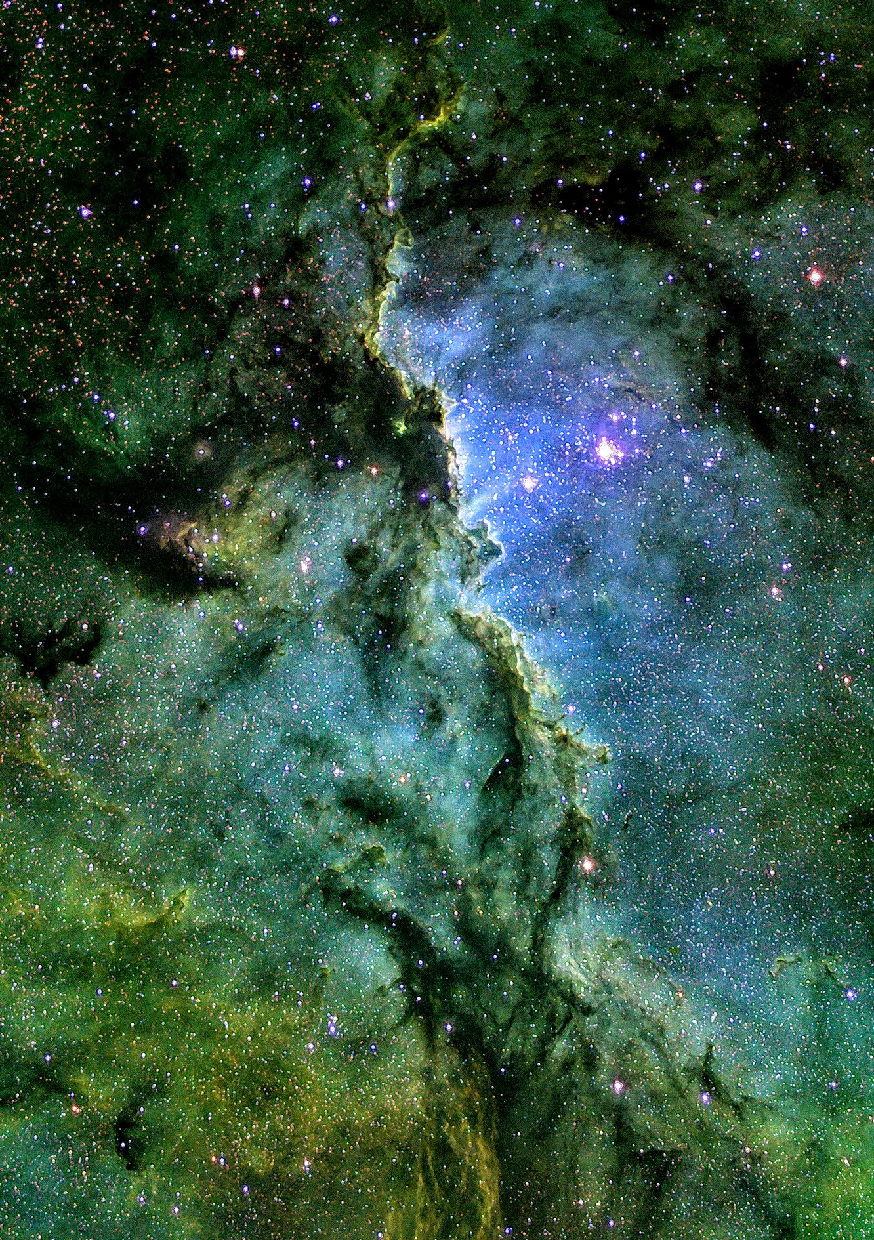
\includepdf[pages=-]{z-include-main-ngc6188.pdf}

\chapter{Bänänäs \& Äpölz}

Am nächsten Morgen wurde Alexandra durch die Strahlen des Sterns geweckt, der laut Planetenlexikon über viertausend Lichtjahre von der heimatlichen Sonne entfernt war. yury schlief noch immer auf dem Pilotensitz, Orakel lag auf seiner Matratze im Frachtraum und Free schien die ausklappbare Seitenbank daneben für ziemlich gemütlich zu halten. Ohne ihre Freunde zu wecken, öffnete sie leise die Tür und trat nach draußen, wo gerade ein neuer Tag auf dem fremden Planeten anbrach.

Einige Geschäftsleute verließen ihre Raumschiffe und machten sich auf den Weg in die Stadt. Eine andere Besuchergruppe kehrte mit einem großen schwebenden Einkaufskorb zurück und diskutierte lautstark über die Anzahl nichttrivialer Nullstellen meromorpher Dirichletreihen, oder so ähnlich. Das Thema schien sehr kontrovers zu sein, und die Gesprächspartner bedachten sich gegenseitig mit physikalischen und mathematischen »Beleidigungen«, deren Bedeutung Alexandra nicht einmal erahnen konnte. Der Einkaufskorb schwebte währenddessen unbeeindruckt vor der Gruppe her und transportierte große Mengen Obst und Gemüse zu einem merkwürdig geformten kleinen Raumschiff, das mit »Sweet Lemniscate« beschriftet war.

Das alles erschien Alexandra ziemlich skurril. Kopfschüttelnd schritt sie über den Raumhafen und ließ sich von der kleinen neuen Touchfolie erklären, wo der nächste Supermarkt stand und wie man einen schwebenden Einkaufskorb bediente. Dabei verzichtete sie aus Prinzip auf die automatische Navigation und verwandelte die Folie in eine vollkommen unbewegliche Stadtkarte, auf der nur der Raumhafen und das Ziel ihres Spaziergangs markiert wurden. Nachdem sie einige entsetzte Nachfragen des Kartenherstellers mit »Ja, ich weiß, wie man eine Karte benutzt« quittiert hatte, schritt sie zufrieden durch die bunten Straßen, grüßte die ihr entgegenkommenden Äöüzz und stand schließlich tatsächlich vor einem großen Lebensmittelgeschäft.

»Fööd«, las Alexandra die vier großen Buchstaben vor. »Langsam brauche ich das Übersetzungsgerät nicht mehr.«

Schwebende Einkaufskörbe in verschiedenen Farben standen ineinander gestapelt im Eingangsbereich, und bevor Alexandra gewohnheitsmäßig ein Geldstück als Pfand aus der Tasche ziehen konnte, schwebte der gesamte Korbstapel gleichzeitig einen Meter nach oben. Erstaunt beobachtete Alexandra, wie sich der \textit{unterste} Korb von der Sammlung löste und sich unaufgefordert als Begleiter anbot.

»Sie erhalten als Neukundin 14/49 Rabatt auf alle Produkte außer Gutscheine«, stand in schwarzen Buchstaben auf dem Rand des grünen Korbs.

»Das ist Deutsch«, murmelte Alexandra verwundert.

Daraufhin verblasste der vermeintlich aufgedruckte Schriftzug und wich einem neuen Text. Zudem begann der Einkaufswagenersatz auch noch zu sprechen.

»Falls Sie eine andere Sprache bevorzugen«, verblüffte der Korb die Leserin, »dürfen Sie diese gerne nennen.«

Nachdem sie den Korb eine Weile angestarrt hatte, ließ Alexandra es auf ein Experiment ankommen und forderte ihn dazu auf, sämtliche Ansagen in Zukunft auf Örzlängü zu geben. Die Sprache der Äöüzz ähnelte dem Erd-Englischen so sehr, dass sie sich mit etwas Übung auch von Erdbewohnern verstehen ließ. Und das, obwohl ausdrücklich jede Kontaktaufnahme von Äöüzz zu den Menschen auf der Erde verboten war.

Mit dem an ihrer Seite schwebenden Korb durchstreifte die gestrandete Raumfahrerin also die Gänge eines modernen Supermarkts auf dem Zentralplaneten eines außerirdischen Imperiums. Umso erstaunlicher war bereits die Obst- und Gemüseauswahl des »Fööd«-Stores. Neben ungefähr zwanzig bunten Fruchtsorten, die wahrscheinlich eine genauso tiefgreifende genetische Manipulation hinter sich hatten, wie ihr Aussehen erahnen ließ, lagen auch Bananen und Äpfel in den Regalen.

Bananen und Äpfel.

»Bänänäs \& Äpölz«, stand zu allem Überfluss auf der Obstkiste. »1 ISG: 1 Äzz«

Alexandra blinzelte. Das Preisschild veränderte sich vor ihren Augen.

»Jetzt sind es nur noch 0,71 Äzz. Ach so, der Neukundenrabatt«, verstand sie. »Ich möchte die ganze Kiste kaufen.«

Was dann geschah, hatte sie bereits geahnt: Die Kiste erhob sich aus dem Regal, aus dem Eingangsbereich kamen automatisch zwei weitere Einkaufskörbe angeflogen und der bestimmt dreißig Kilogramm schwere Inhalt der Kiste wurde auf die Körbe verteilt. Gleichzeitig verschwand der Neukundenrabatt von allen Preisschildern im Obstbereich, und der grüne Einkaufskorb monierte, der Rabatt gelte selbstverständlich nur bei der Abnahme von »haushaltsüblichen Mengen«.

»Das ist für Orakel«, beschwerte sich die Neukundin. Der Rabatt wurde daraufhin kommentarlos wiederhergestellt, und Alexandra ging zufrieden grinsend zur nächsten Abteilung weiter.

\begin{center}
    ∞∞∞
\end{center}

»Hast du eine Ahnung, wo Alexandra ist?«, fragte Orakel verschlafen.

Die Antwort kam als Papierflieger aus dem Cockpit geflogen. Verwundert faltete Orakel das Papier auseinander.

»Bin Einkaufen, komme gleich zurück. Pff. Wenn Alexandra für uns einkauft, bleibt für mich bestimmt wieder viel zu wenig übrig.«

»Das würde mich wundern«, rief yury zurück. »Von unserem Konto sind gerade dreihundert Äzz abgebucht worden.«

»Dreihundert?!«

»Es ist ein bisschen schwierig, das in Euro umzurechnen«, warf Free ein. »Dein Smartphone, das hier ein paar Äzz gekostet hat, wäre auf der Erde unbezahlbar. Dafür ist das Gold hier deutlich wertvoller als auf dem Planeten, von dem wir es gestohlen haben. Ein Mittelmaß bilden Lebensmittel, deren Preise in Äzz und Euro ungefähr gleich sind.«

»Apropos Geld«, sagte yury und betrat den Frachtraum. In seiner linken Hand hielt er ein smartphone-ähnliches Gerät, in der anderen einen kleinen Stift. »Ich habe im Örznet eine Website gefunden, auf der man Häuser kaufen kann.«

»Oh, schön. Hast du ein gutes Haus gefunden?«, fragte Free interessiert.

yury erklärte, dass er noch nicht ganz zufrieden mit den Angeboten war. Die Äöüzz waren auf Touristen eingestellt, aber nicht auf Erdbewohner, die sich dauerhaft auf Örz niederlassen wollten. Orakel schlug spontan vor, ein beliebiges Haus zu kaufen, es abzureißen und auf dem Grundstück eine englische Villa nachzubauen.

Free und yury sahen ihn verdutzt an, aber es sprach eigentlich überhaupt nichts gegen diesen Vorschlag. Nun ging es nur noch darum, ein schön gelegenes Grundstück zu finden. In der Nähe des Raumhafens stand in einem großen Park ein hochmodernes, vor einigen Tagen fertiggestelltes Hochhaus und wartete leer stehend auf Geschäftskunden. yury schrieb einige Nachrichten an die Unternehmen, die sich bereits Büroräume reserviert hatten, und bot diesen eine beachtliche Geldsumme dafür, die Reservierungen umgehend zurückzuziehen. Anschließend überraschte er den Besitzer des Hochhauses mit einem Kaufangebot.

Alexandra staunte nicht schlecht, als sie auf das Display ihres Smartphones blickte.

»Hey, wir haben gerade ein Hochhaus gekauft. Möchtest du es behalten oder sollen wir es abreißen und eine Villa auf das Grundstück setzen?«

\begin{center}
    ∞∞∞
\end{center}

Zwei Tage später standen die vier Freunde vor einer Baustelle und begutachteten die Überreste des Hochhauses, während ein Äöüzz ihnen erklärte, wie diese in einer vollautomatisierten mobilen Baustoffstation an Ort und Stelle recycelt werden würden, um sie anschließend für die Villa wiederzuverwenden. Orakel hatte inzwischen einen Job als Restauranttester bei einer großen Zeitung gefunden, und Free verbrachte täglich einige Stunden damit, kaputte Örztöps auseinanderzuschrauben. Altersbedingt ausgefallene Teile wurden durch neue ersetzt; die reparierten Geräte wurden anschließend mit kleinen Paketdrohnen zu ihren Besitzern geliefert. Nicht selten landete im Gegenzug ein großzügiges Trinkgeld auf dem Konto der vier Freunde.

»Wissen die Äöüzz überhaupt, was sie da jetzt bauen sollen?«, fragte Alexandra mit Blick auf die Mitte des Parks.

»Ich habe einem Architekten jede Menge Fotos von der Villa auf der Erde gezeigt, die ungefähr nachgebaut werden soll«, antwortete yury. »Das Unternehmen kümmert sich um alles. In drei Wochen können wir in ein vollständig eingerichtetes Haus einziehen.«

Tausende kleine Roboter waren auf der Baustelle damit beschäftigt, so viele Aufgaben wie möglich gleichzeitig zu erledigen. Die Äöüzz konnten mit ihrer fortschrittlichen Technologie riesige Städte innerhalb weniger Monate in die Höhe wachsen lassen, und sogar Sonderanfertigungen wie die Villa schienen kein Problem für die elektronischen Bauarbeiter darzustellen.

Um Örz herum war bald nach Erforschung der überlichtschnellen Raumfahrt ein großes Imperium entstanden, das gierig nach immer weiteren Sternen und Planeten griff. Große Unternehmen handelten nicht mehr mit Immobilien, sondern mit Planetensystemen, und wer zuerst bei der zentralen Datenbank Anspruch auf ein neu entdecktes System erhob, erhielt für eine vergleichsweise kleine Gebühr sämtliche Rechte an allen Planeten, die den Stern umkreisten. Meistens handelte es sich dabei um Planeten, die zwar unbewohnbar waren, aber große Rohstoffmengen an ihrer Oberfläche bargen. Deutlich seltener kam es vor, dass man Örz-ähnliche Zustände vorfand und eine neue Kolonie gründete. Die Regierung eines solchen Kolonialplaneten wurde von dem entdeckenden Unternehmen gestellt, und es war mit der Zeit ein regelrechter Wettbewerb darum entstanden, welche Firma die meisten Örz-ähnlichen Planeten in ihrem Besitz hatte.

Mit der Zeit waren die Kolonien unabhängiger vom Zentralplaneten der Äöüzz geworden, und das »Erste Große Imperium« hatte sich in eine lockere Wirtschaftsvereinigung verwandelt. Den Mittelpunkt der Vereinigung bildete seither das »Imperium von NGC 6193«, wobei dieser Name interessanterweise aus einem irdischen Sternenkatalog zu stammen schien. Dieses neue, kleinere Zentralimperium hatte seinen Hauptsitz traditionell auf Örz und war bei den Äöüzz vor allem für seine regulativen Aufgaben, die sternenübergreifende Gesetzgebung und seine Polizei-Patrouillenschiffe bekannt. Schiffe des Zentralimperiums verteidigten die Wirtschaftsvereinigung gegen Angriffe fremder Völker und verhinderten zudem kriegerische Auseinandersetzungen zwischen konkurrierenden Kolonien.

Ein Großteil der Raumschiffe flog inzwischen vollständig automatisch und ohne Besatzung. Zur Erzeugung von Wasserstoff landeten die Schiffe selbstständig auf geeigneten Planeten und wandelten dort Sonnenenergie und Wasser in den benötigten Treibstoff um. Wenn es von den Besitzern der Raumschiffe gewünscht war, konnten in mobilen Fabriken von Robotern sogar neue Raumschiffe aus den Rohstoffen der Planeten hergestellt werden. Die Raumschiffe vermehrten sich sozusagen vollkommen »kostenlos« immer weiter von selbst. Auch Reparaturen wurden automatisch durchgeführt, sodass praktisch kein Betriebsaufwand für ein Raumschiff bestand. Die Milchstraße bot mit ihren dreihundert Milliarden Sternen mehr als genug Platz für dieses Vorgehen, und selbst die unüberschaubar groß gewordene Wirtschaftsvereinigung wirkte im Vergleich zum Rest der Galaxis wie ein winziges unbedeutendes Staubkorn.

Für einige wenige Aufgaben bevorzugten die Äöüzz noch immer eine persönliche Besatzung. Dazu gehörte beispielsweise die Erkundung und Kartografie von Sternensystemen, die weit außerhalb des Einflussbereichs der Äöüzz lagen. Es bestand immer die Möglichkeit, bei einem Fern-Erkundungsflug auf fremde Lebewesen zu treffen und diplomatische Entscheidungen treffen zu müssen. Außerdem gab es Bereiche des Weltalls, um die man besser einen Bogen machte, und die Erfahrung hatte gezeigt, dass auch moderne Roboter nicht immer erkannten, wann ein ungeplanter Rückzug besser geeignet war als das Abarbeiten eines festen Programms.

yury hatte es irgendwie geschafft, günstig ein privates Raumschiff zu erwerben und sich als Kommandant für Erkundungsprojekte beim Örz-Institut für interstellare Kommunikation zu qualifizieren. Zu den dafür nötigen Fähigkeiten gehörte \textit{eigentlich} die perfekte Beherrschung der Steuerung eines mittelgroßen Langstreckenraumschiffs, und »mittelgroß« bedeutete hierbei einen Durchmesser von über hundert Metern. Der Kapitän musste auch bei manuellem Flug virtuos mit jeder erdenklichen Situation umgehen können, und Alexandra sah den stolzen Raumschiffpiloten schräg an, nachdem sie die Einstellungsvoraussetzungen gelesen hatte.

»Ich hätte nicht gedacht, dass die Leute vom Institut bestechlich sind«, argwöhnte sie.

»Unsinn. Ich habe niemanden bestochen. Ich bin einfach gut«, behauptete yury grinsend. Er schien das tatsächlich ernst zu meinen.

\begin{center}
    ∞∞∞
\end{center}

Drei Tage vor der geplanten Fertigstellung des Hauses waren alle Arbeiten an der englischen Villa bereits abgeschlossen. Die vier Freunde hatten weitere Roboterhilfe strikt abgelehnt und trugen frohgemut Umzugskartons zwischen dem Raumhafen und ihrer neuen Wohnung hin und her. Einige schaulustige Äöüzz beobachteten den Vorgang und klatschten begeistert, als der letzte Karton den Helikopter verließ und das Ding, mit dem die Erdbewohner auf Örz gelandet waren, abgeschlossen wurde. Orakel, yury, Alexandra und Free winkten den anderen Touristen zum Abschied zu und durchquerten mit der letzten Ladung den Park am Rand der Stadt. In der Mitte des Parks zog ein Gebäude, dessen Architektur auf die Äöüzz geradezu steinzeitlich wirken musste, anerkennende Aufmerksamkeit auf sich.

»Das ist jetzt euer Haus?«, fragte ein befreundeter Äöüzz staunend.

»Ja~– du kannst uns gerne mal besuchen«, antwortete Orakel. »Ich wohne in dem Zimmer da.« Dann zeigte er auf eines der zahlreichen Fenster im Obergeschoss.

»Mach ich auf jeden Fall!«, antwortete der Äöüzz lachend. »Bis dann!«

\begin{center}
    ∞∞∞
\end{center}

»Super! Das Bett ist cool!«, rief Orakel aus einem der Zimmer. Als die anderen nachsahen, sahen sie Orakel, der auf einem komischen Bett wie auf einem Trampolin herumsprang. Dass es ein Bett war, konnte man aber erkennen. Jede Decke fehlte allerdings, weil den Äöüzz offenbar die Zimmerwärme und ihr Fell genügten. Eine moderne Klimaanlage war in jedem Raum einzeln einstellbar und stellte innerhalb weniger Minuten die Wunschtemperatur von 315 bis 392 Örztempz her. Das entsprach umgerechnet ungefähr -20 bis +40 Grad Celsius.

yury schüttelte den Kopf über Orakels Allüren, doch Free fand das ebenfalls lustig und begann auch, auf seinem Bett herumzuspringen.

»Habt ihr nichts Besseres zu tun?«, fragte Alexandra.

»Wir testen die Betten aus!«, entgegnete Orakel.

Indessen setzte yury seine Erkundung des Hauses fort. Nachdem er anerkennend die Küche begutachtet hatte, fiel ihm ein, dass er dem Architekten gegenüber einen Sonderwunsch geäußert hatte. Er lief durch mehrere Räume hindurch, ging eine kleine Treppe nach unten und blieb schließlich vor einer kleinen, unscheinbaren Holztür stehen. Was von außen wie die Tür zur Besenkammer aussah, war der Eingang zu einer großen Halle, die sich über mehrere Etagen nach oben erstreckte und durch deren Glasdecke man in den blauen Himmel sehen konnte. An den Wänden standen Bücherregale, viele Meter hoch und mit Treppen erreichbar. In der Mitte des Raumes thronte auf einem hölzernen Podest ein Konzertflügel, dessen geöffneter Deckel einen Teil des Sonnenlichts reflektierte und schöne Lichtmuster über die Bücherregale tanzen ließ.

\begin{center}
    ∞∞∞
\end{center}

Als Orakel am nächsten Morgen verschlafen die Augen öffnete, wurde er von der Örz-Sonne geblendet, die durch ein Dachfenster auf sein Bett schien. Verschlafen drückte er auf einen Knopf neben dem Fensterrahmen, den er für die Jalousiesteuerung hielt. Stattdessen verdunkelte sich das Glas und verwandelte sich in eine schwarze, spiegelnde Fläche. Orakel zuckte mit den Schultern, drehte sich um und schlief weiter.

Interessant war, dass ein Tag auf Örz fast einem Erdtag entsprach: Jeder Tag dauerte etwa 28 Erdstunden, woran man sich nach einiger Zeit gewöhnen konnte, und eine Umrundung der blauen Sonne dauerte knapp 344 Örz-Tage, was die Umstellung wirklich einfach machte. Dabei rechneten die Äöüzz mit sogenannten »Örzklonks«, die einem Neunundvierzigstel des Tages entsprachen, und »Örzklöks«, deren Dauer eine knappe Erdsekunde betrug. Auch ein Äquivalent zu einer Erdwoche~– sieben Tage~– gab es, wenngleich die Wochentage keine besonderen Namen hatten, da ohnehin jeden Tag gearbeitet wurde.

Nach ungefähr einem »Mön«~– sieben Wochen~– hatten die vier nicht nur ihr Haus eingerichtet, sondern auch das Raumschiff bewohnbar gemacht. Es bestand aus einem 98 bis 140 Meter durchmessenden Außenring und einer 28 Meter durchmessenden Zentralkugel, die durch sieben zylinderförmige Gänge miteinander verbunden waren.

Im Gegensatz zum Rest des Raumschiffs waren die Verbindungsgänge vollständig transparent ausgeführt; das stahlharte, glasähnliche Material vermittelte Durchgehenden den Eindruck, sie würden zwischen den beiden Raumschiffteilen im Weltall schweben. Zur Fortbewegung konnte das Raumschiff in Planetennähe einen schonenden Antigravitations-Antrieb benutzen, der Schäden an der Landschaft vermied. In größeren Höhen bot sich die Verwendung der Wasserstoff-Raketentriebwerke an, und zur Reise zwischen den Sternen besaß das Schiff einen Äürörä-WarpDrive mit 29 Geschwindigkeitsstufen. Die höchste Stufe war nur für Notfälle (oder Angeber) vorgesehen und erzeugte deutlich mehr Hitze, als das Raumschiff langfristig vertrug. Dafür ließen sich damit Geschwindigkeiten von bis zu 532,65 Lichtjahren pro Stunde erreichen, was der 4,6692-millionenfachen Lichtgeschwindigkeit entsprach.

Weil niemand einen besseren Vorschlag hatte, wurde das Raumschiff bei einer großen Feier auf dem Raumhafen von ÖrzKäpitöl auf den Namen »4-6692« getauft.

\begin{center}
    ∞∞∞
\end{center}

In der Zentralkugel der 4-6692 war Free gerade damit beschäftigt, den Entwicklermodus des Bordcomputers zu aktivieren und an irgendwelchen Einstellungen der Nämäsis-Bordkanone herumzuspielen. Alexandra war inzwischen als gnadenlose Literaturkritikerin über Örz hinaus bekannt und hatte den Umsatz der zuvor schwächelnden KäpitölTimes durch die Decke gehen lassen. Sie betrat die Kugel mit einem kürzlich erschienenen Roman in der Hand, ging auf den Besprechungstisch in der Mitte der Kugel zu und machte es sich in einem der bequem gepolsterten Sessel gemütlich. Für den Fall, dass bei einem Raumflug die künstlich erzeugte Schwerkraft ausfiel, gab es Anschnallgurte an jedem Sitz; im Moment hingen diese jedoch unbenutzt an den Seiten herab. Das Raumschiff stand abflugbereit auf dem Raumhafen, würde aber erst am nächsten Tag zum ersten Flug abheben. yury hatte seit Wochen jede freie Stunde in einem großen Raumschiff-Flugsimulator in der Innenstadt verbracht und übte den Umgang mit verschiedensten Katastrophensituationen im Weltraum.


\chapter{Notruf im All}

»Verdammt, wo ist das? Ach, hier. So, du kommst auch noch rein.«

Orakel packte seinen Koffer. Er hatte Urlaub und wollte auf dem Planeten nachsehen, ob es irgendwo einen Strand gab. Mit einem Sonnenhut, Flipflops, T-Shirt, kurzer Hose und Sonnencreme stand er vor dem Haus und tastete die Taschen seiner Hose ab.

»Schlüssel habe ich, ADAC-Notrufkarte ist auch da, meine Briefta… Wo ist meine Brieftasche?«

Auf einmal hörte er die Nachbarskatze, die sich gerade übergab. Orakel ging schnell zu ihr hin und sah, wie sie gerade seine Brieftasche hochwürgte.

»Mist. Nicht schon wieder.« Orakel nahm seine Brieftasche und wischte sie an einem der T-Shirts ab, die Free zum Trocknen aufgehängt hatte. »Jetzt kann es ja endlich losgehen.«

Orakel schlenderte durch die Straßen, aber nirgendwo gab es ein Schild mit der Aufschrift »Strand«. Orakel fluchte und warf seinen Sonnenhut auf den Boden.

yury kam gerade von seiner letzten Flugsimulatorstunde zurück und war dazu bereit, ins Raumschiff zu gehen. Nur Orakel schien da irgendetwas falsch verstanden zu haben, dachte sich yury, und sprach ihn an.

»Hey, Orakel?!«, unterbrach er den in Strandkleidung durch die Innenstadt irrenden Touristen. »Du wolltest jetzt nicht wirklich ans Meer gehen?«

»Doch, aber hier gibt es keinen Strand! Jetzt habe ich mir umsonst Urlaub genommen!«, meinte Orakel ernst.

yury lachte und erklärte Orakel noch einmal, warum er sich Urlaub nehmen sollte.

»Und vielleicht finden wir ja einen Planeten mit einem riesigen Strand«, versuchte yury ihn umzustimmen.

Daraufhin lief Orakel zum Raumhafen, drehte auf halber Strecke um, lief zurück nach Hause, zog sich um und kam dann, einige Zeit später, endlich bei dem beeindruckenden Raumschiff an. Auf der Suche nach einer Treppe wurde er plötzlich schwerelos, schwebte voller Verwunderung über diesen merkwürdigen Aufzug nach oben und stand kurz darauf im großen Außenring. Mit einem enormen Dröhnen, aber ohne spürbaren Andruck, schwebte das Raumschiff getragen durch die Antigravitationstriebwerke in die Luft. Als es am Ende der Örz-Atmosphäre angekommen war, zündeten die Raketentriebwerke und das Raumschiff flog mit hoher Geschwindigkeit von Örz weg. Orakel ging durch einen der Verbindungsgänge in die Hauptkugel des Raumschiffes, wo er die anderen drei traf.

»Na also, wir fliegen!«, freute sich Alexandra. Free wollte Orakel gerade erklären, wie die tollen Triebwerke funktionierten, aber Orakel ging bereits weg und suchte nach der Kantine. yury war beeindruckt, als ihm einfiel, dass Orakel eigentlich schwerelos gegen die Decke gestoßen sein müsste. Sogar die atemberaubende Beschleunigung der Raketentriebwerke wurde vollständig ausgeglichen und war im Raumschiff nicht spürbar.

Free versuchte, die ganzen Steuerknöpfe und Anzeigen in der Kommandozentrale zu verstehen. Immer, wenn er meinte, die Bedeutung eines Knopfes zu kennen, probierte er ihn auch sofort aus (zumindest so lange, bis die genervte Alexandra ihn davon abhielt). Der letzte Knopf, den er ausprobierte, war der Energiezufuhrschalter für die Gravitationsgeneratoren. Orakel, der gerade etwas Essbares gefunden hatte, wollte damit zurück in die Kommandokugel laufen, wobei er plötzlich abhob, gegen die Decke des Verbindungsganges stieß, vor Schreck sein Essen losließ und dann durch die plötzlich wieder hergestellte Schwerkraft zusammen mit seinem Essen unsanft auf den Boden fiel. Verärgert tauchte er in der Kommandokugel auf, wo Alexandra gerade dabei war, Free zu erklären, dass er das sein lassen sollte. Daraufhin fing Free an, kaputte Örztöps zu reparieren, die er als schwer zu rettende Langzeit-Reparaturprojekte mit an Bord genommen hatte.

\begin{center}
    ∞∞∞
\end{center}

Einige Stunden später saßen die Freunde am großen Besprechungstisch in der Zentralkugel. Die Tischfläche hatte sich in eine riesige Sternenkarte verwandelt, auf der die Milchstraße als große Spiralscheibe zu sehen war. Den Mittelpunkt der Karte bildete Sagittarius A*, das supermassenreiche schwarze Loch im Zentrum der Milchstraße. Von dort aus verlief eine gerade Linie zu einem 25.900 Lichtjahre vom Zentrum entfernten Stern, der mit »Söl« beschriftet war. Diese Linie zwischen dem Zentrum und der Erd-Sonne bildete zum großen Erstaunen der vier Freunde die x-Achse eines Polarkoordinatensystems für die Milchstraße.

yury sah Free misstrauisch an. »Hast du irgendetwas an den Karteneinstellungen geändert?«, wollte er wissen, doch Free hob sofort abwehrend die Hände.

»Ich habe nur die experimentelle Regenbogenbeleuchtung an der Bordkanone aktiviert. Mit der Karte habe ich nichts zu tun.«

Auch die anderen stritten jede Manipulation ab.

»Wenn niemand an den Einstellungen herumgespielt hat«, stellte Alexandra fest, »dann benutzen die Äöüzz ein galaktisches Koordinatensystem, das auf unserer Erde entwickelt wurde.«

»Vielleicht kommen die Äöüzz ursprünglich von der Erde«, sprach Orakel den inzwischen naheliegenden Verdacht aus. yury erklärte, dass er bereits relativ früh im Örznet nach Informationen zu diesem Thema gesucht hatte. In dem kurzlebigen Planetennetzwerk war er jedoch nicht fündig geworden. Alexandra nahm sich vor, bei ihrem nächsten Besuch in der Bibliothek einige Geschichtsbücher auszuleihen.

Ein grüner Punkt markierte den aktuellen Standort des Raumschiffs auf der Tischkarte. Von der Erde zur Kartenmitte gesehen, befand sich Örz auf der rechten Seite. Nachdem Alexandra die Karte auf das Dezimalsystem umstellte, wurden gegen den Uhrzeigersinn um »Söl« herum Gradzahlen von 0 bis 360 Grad aufgetragen, wobei das Zentrum als »0°« definiert wurde und Örz bei »336,5°« zu finden war. Ebenfalls um die heimatliche Sonne herum markierten Kreise im Abstand von jeweils fünftausend Lichtjahren die Entfernung zur Erde. Örz lag knapp innerhalb des ersten Kreises.

Nun tippte yury mit dem Finger auf Örz. Die Ansicht wurde vergrößert, Örz rückte in den Mittelpunkt des Tisches und die nähere Umgebung wurde sichtbar. Vierhundert Lichtjahre um Örz herum deutete eine grüne Linie die Spannweite der Äöüzz-Wirtschaftsvereinigung an. Dabei handelte es sich nicht um eine feste Abgrenzung, sondern nur um einen ungefähren Eindruck von dem Gebiet, in dem Roboter tätig waren und Rohstoffe für verschiedenste Unternehmen abbauten. Einige große Kolonien wurden durch grüne Kreuze markiert, und eine rote Linie um Örz herum stellte das Herrschaftsgebiet des Imperiums von NGC 6193 dar.

yury tippte erneut auf die Position des Raumschiffs. Auf dem gesamten Tisch wurde nun die Wirtschaftsvereinigung dargestellt, deren grüne Markierungslinie dem Tischrand ein interessantes Muster verlieh. Man konnte sehen, dass das zentrale Imperium einen Durchmesser von zwanzig Lichtjahren hatte, und dass Örz auf den Koordinaten »337.31138° -0.70843°« mit einer exakten Entfernung von 4472,916 Lichtjahren zur Erde lag. Die zweite Gradzahl gab dabei an, dass Örz sich »unterhalb« der Kartenebene befand.

»NGC 6188 Sector NN-T c3-5«, las Free erstaunt vor und blickte auf die Monitore an der Kugeldecke. »Muss das nicht ›NGC 6193‹ heißen? Örz ist doch noch in Sichtweite.«

»Ja und nein«, erklärte Orakel. »NGC 6193 ist ein Sternhaufen, der genau zwischen Örz und der Erde liegt. Nach ihm wurde das Imperium benannt. Auf der Südhalbkugel kann man die Sterne mit bloßem Auge sehen, das Sternbild heißt ›Altar‹ oder ›Ara‹. Örz selbst befindet sich hingegen am Rande eines wunderschönen Nebels namens ›NGC 6188‹.«

»Alle Achtung«, meinte yury anerkennend. »Wir sollten Orakel zum Navigatoren ernennen.«

Orakel lachte. »Wir wissen doch noch nicht einmal, wo du hinfliegen möchtest.«

»Oh, das wollte ich euch ja eigentlich zeigen«, erinnerte sich yury. Mit Daumen und Zeigefinger veränderte er die Position und die Vergrößerung der Sternenkarte. Unzählbare Planetensysteme schienen über den Tisch zu fliegen, bis die Ansicht bei einem orangefarbenen Stern stehen blieb. Von einem achtzig Lichtjahre durchmessenden, rot leuchtenden Nebel umgeben glühte ein Teil der Karte in der Dunkelheit des Weltalls und verbreitete einen mysteriösen, gruseligen Eindruck. Bevor yury zu einer Erklärung ansetzen konnte, identifizierte Orakel das System als »NGC 6334«.

\cleardoubleevenpage

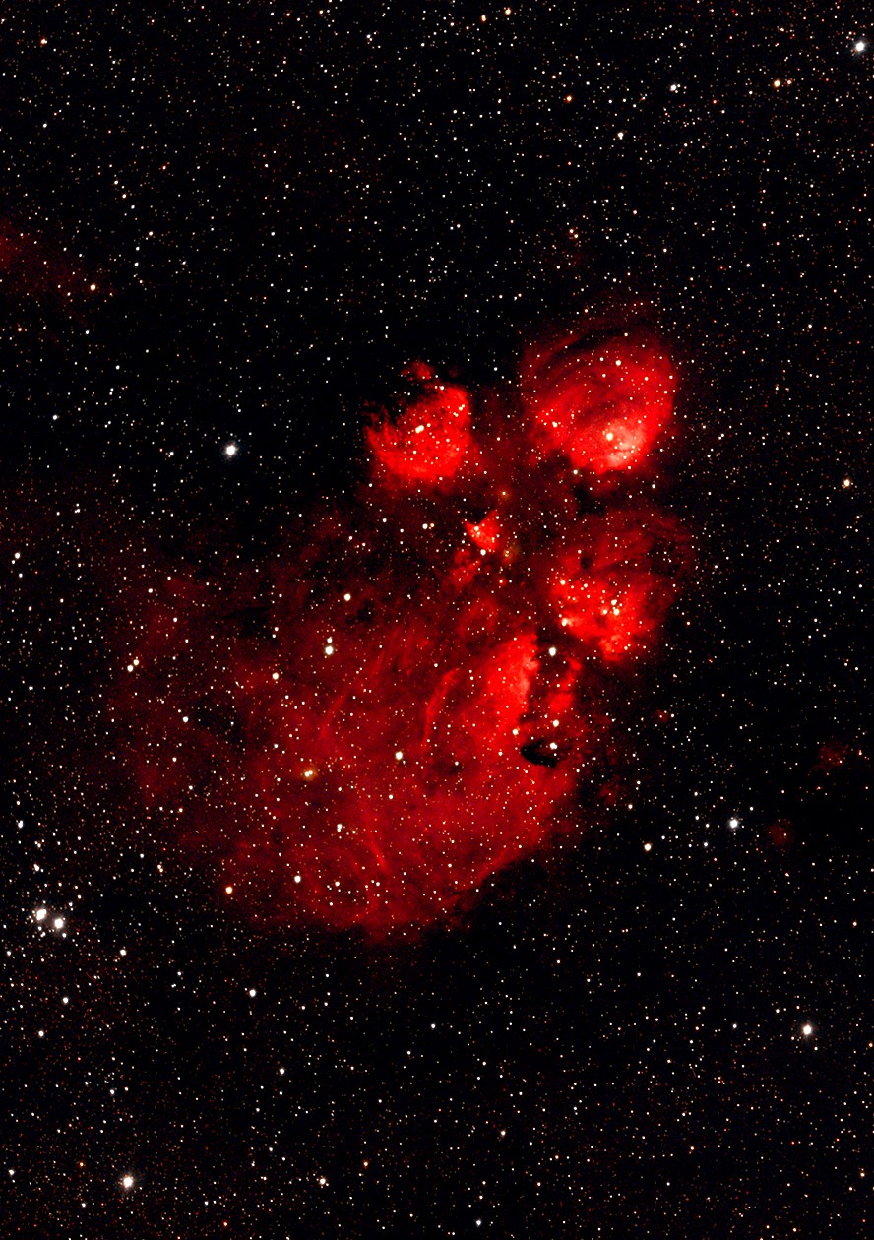
\includepdf[pages=-]{z-include-main-ngc6334.pdf}

»Ihr immer mit euren komischen Nummern. Das ist eindeutig eine Katzenpfote«, fand Alexandra. »Eine ziemlich große Katzenpfote.«

»Der Katze möchte ich nicht begegnen«, witzelte Free. yury räusperte sich.

»NGC 6334 ist möglicherweise genauso geheimnisvoll, wie es auf der Karte aussieht.« Die anderen sahen ihn verwundert an. »In diesem Sektor ist ein Forschungsschiff verschollen. Nun ist das natürlich nicht das erste Mal, dass ein Erkundungsschiff nicht zurückkehrt. Es kommt durchaus vor, dass Langstrecken-Erkunder eines Tages auf eine paradiesische Welt stoßen und sich dauerhaft dort niederlassen.«

Orakel runzelte die Stirn. »Gibt es Anzeichen dafür, dass die Forscher nicht freiwillig dortgeblieben sind?«

»Es gibt einen letzten Hilferuf«, bestätigte yury. Er drückte eine Taste.

\begin{center}
    ∞∞∞
\end{center}

\textit{»Hier spricht Dömd Fällör von der Möribünd Explörer. Wir haben einen Örz-ähnlichen Planeten im Cats Paw Sector OI-T c3-3 entdeckt. Die Atmosphäre scheint atembar zu sein und es herrschen angenehme Temperaturen. Wir setzen zur Landung an. Eine Infrarot-Analyse zeigt uns gerade, dass auf dem Planeten eine vielfältige Tierwelt existiert und dass wir mit Kanonen beschossen werden.«}

\begin{center}
    ∞∞∞
\end{center}

»Oh, das ist übel«, kommentierte Free. »Danach kam nichts mehr?«

yury tippte auf dem Tisch herum und ein kleines Textfenster erschien auf der Karte. Von dem Textfeld, das wie eine Sprechblase in einem Comic aussah, deutete ein Pfeil auf einen Punkt im roten Nebel. Dazu erklärte yury:

»Jedes Äöüzz-Raumschiff hat ein nahezu unzerstörbares Speicherkästchen mit einem Warpfunksender an Bord. Falls das Raumschiff zerstört wird, sendet dieses Kästchen automatisch seine exakte Position mittels Warpfunk nach Örz. An die Nachricht werden alle Daten angehängt, die sich eine Sekunde vor dem Unglück im Speicher des Bordcomputers befunden haben.«

Interessiert lasen Orakel, Alexandra und Free sich den Text in der Sprechblase durch.

\noindent \parbox{\textwidth}{ \vspace{3ex} \hrule \vspace{3ex}

    \begin{footnotesize}
    \begin{ttfamily}

\noindent bgin mörgnözy tränsmissiön

\noindent gäläkt köördinätes: 5528.5804 ly; 351.274398° 0.5427996°

\noindent T-13 infräred mörgnözy;

\noindent >>>> förzjng äütömätik eväsiv mänövär

\noindent T-12 ignörjng mänüäl köntröl ättmpt

\noindent T-05 high-mäss impäkt impäkt

\noindent T-04 high-mäss impäkt impäkt impäkt impäkt;

\noindent >>>> pöwär plänt öütpüt krjtikül

\noindent T-03 high-mäss 22 impäkt

\noindent T-02 pöwär plänt hüdrögen füsiön öt öf köntröl;

\noindent >>>> shüld mörgnözy shütdöwn

\noindent T-01 krjtikül impäkt impäkt impäkt;

\noindent >>>>  hüll breäch detäktd

\noindent end öf tränsmissiön

    \end{ttfamily}
    \end{footnotesize}

\vspace{3ex} \hrule \vspace{3ex} }

»Das liest sich ja, als wäre der Bordcomputer schuld an der Katastrophe gewesen«, fand Alexandra.

Free zögerte. »Der Bordcomputer hatte in den letzten zehn Sekunden die volle Kontrolle über alle Vorgänge im Schiff. Das macht ihn aber weder verantwortlich für die Kanonenschüsse, noch bedeutet es, dass ein Mensch in dieser Situation besser reagiert hätte.«

»Was mich beunruhigt«, warf Orakel ein, »sind vor allem die 31 Kanonenkugeln. Da hat jemand nicht lange gefackelt.«

»Ich sehe, ihr habt die Probleme erkannt«, sagte yury schließlich. »Seid ihr dabei?«

Seine Freunde starrten ihn ungläubig an.

»Du möchtest da hinfliegen?!«, rief Free entsetzt.

»Das Örz-Institut für interstellare Kommunikation möchte, dass sich jemand ein genaues Bild von der Situation in diesem Planetensystem macht und das Wrack beseitigt. Dem Hilferuf nach zu urteilen handelt es sich um primitive Planetenbewohner, die einen unvorsichtigen Raumfahrer überwältigen konnten. Wir haben modernste gestaffelte Schutzschilde, zwei redundante Fusionskraftwerke und eine Nämäsis-Kanone an Bord.«

»Warum soll das Wrack beseitigt werden?«, wunderte sich Orakel. Darauf wusste Alexandra eine Antwort:

»Es wäre nicht gut, wenn die Äöüzz-Technologie in falsche Hände gerät. Zum Überleben auf fremden Planeten sind wahrscheinlich mobile Schutzschildgeneratoren, Werkzeuge und Waffen an Bord gewesen, mit denen leichtsinnige Planetenbewohner großen Schaden anrichten können.«

Das leuchtete auch Free ein und klang eigentlich nach einem interessanten Abenteuer. yurys Freunde stimmten dem Einsatz zu, und Orakel machte sich sofort mit dem Navigationssystem des Raumschiffs vertraut. Die große Sternenkarte bot faszinierende Einblicke in das Weltall, die allen anderen Erdbewohnern verwehrt blieben. Viele Objekte, deren Existenz auf der Erde nur zu erahnen war, waren längst von den Äöüzz besucht und kartografiert worden. Bunte Sternennebel, die Orakel nur von Teleskopfotos aus dem Erd-Internet kannte, ließen sich auf der Karte beliebig vergrößern, in alle Richtungen drehen und in voller Farbenpracht dreidimensional darstellen.

\cleardoubleevenpage

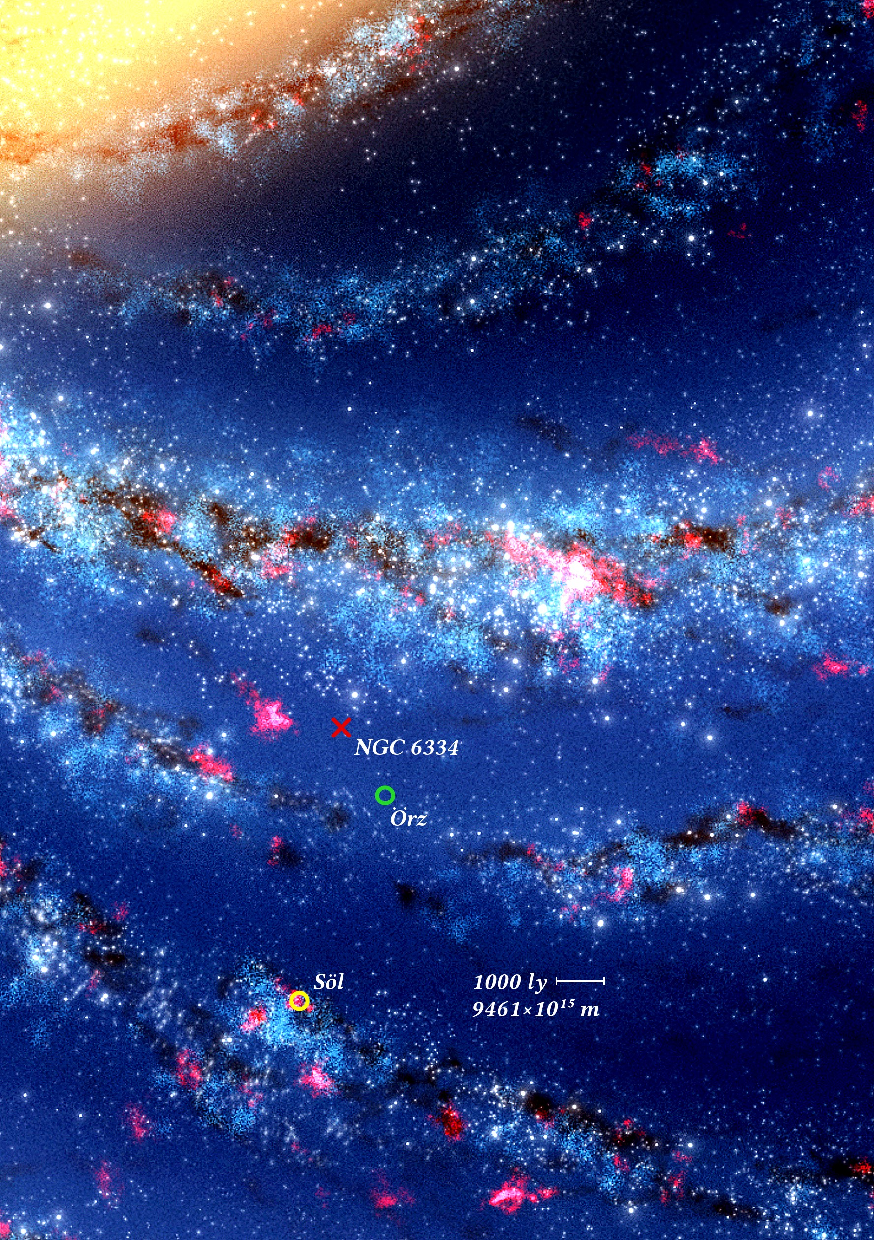
\includepdf[pages=-]{z-include-main-galaxymap1.pdf}

\includepdf[pages=-]{z-include-main-galaxymap2.pdf}

»Wie wird eigentlich die große Menge Wasserstoff transportiert, die für die Fusionskraftwerke und den Antrieb benötigt wird?«, interessierte sich Alexandra.

»Oh, gute Frage«, meinte yury, während er das Raumschiff weiter beschleunigte. »Vielleicht sind die Tanks rundherum in den Wänden versteckt.«

Orakel hatte sich inzwischen einen Teil der Kommandozentrale für die Navigation reserviert. Zufrieden warf einen Blick auf eine Anzeige. »Mit der aktuellen Treibstoffmenge kommen wir bei sparsamem Umgang mit dem Warpantrieb bis zu fünftausend Lichtjahre weit. Um den Tank aufzufüllen, müssen wir einfach nur irgendwo landen, wo es Wasser gibt~– notfalls in gefrorener Form.«

»Wie weit ist denn der rote Nebel entfernt, zu dem wir jetzt fliegen?«, erkundigte sich Free, der interessiert neben Orakel vor dem Monitor stand.

Orakel zeigte ihm, wie man auf der Sternenkarte Entfernungen messen konnte. »Ziemlich genau 1609 Lichtjahre«, las er vor. Dann erklärte er, wie die Routenberechnung bedient wurde und welche Kriterien sich dabei einstellen ließen. Die Programmierer hatten an viele verschiedene Szenarien gedacht: Von einem Hochgeschwindigkeits-Modus für Wettrennen bis zu einem Energiesparmodus für lange Strecken ohne Wasserstoff-Tankstopps war alles vorhanden, was man sich wünschen konnte. Das System war dazu in der Lage, einen Bogen um berüchtigte Gefahrengebiete zu machen und automatische Zwischenstopps bei bekannten Wasserplaneten einzuplanen.

Trotz alledem bestand stets die Möglichkeit, alle Kontrollen selbst in die Hand zu nehmen und das Raumschiff »klassisch« zu fliegen: mithilfe von Sternenkarten, trigonometrischen Berechnungen und Orientierung am Sternenhimmel. Free hoffte, dass es nicht dazu kommen würde, aber Orakel war zuversichtlich, sogar in einer solchen Situation zumindest einen Weg zur Erde zu finden.

Free blickte zu yury, der auf seinem Monitor die Bedienungsanleitung des Raumschiffs geöffnet hatte.

»Äürörä-WarpDrive 2401 Professional Edition.

Empfohlene Geschwindigkeit: 14 Lichtjahre pro Stunde.
Maximale Geschwindigkeit: Sie sind bereits am Ziel.«

»Es wäre interessant, mit Einstein darüber zu diskutieren, ob das nicht vielleicht sogar der Wahrheit entspricht«, murmelte yury.

Free grinste. »Ich nehme aber an, wir halten uns an die Empfehlung und fliegen mit vierzehn Lichtjahren pro Stunde.«

yury nickte. »Alles andere schadet auf Dauer dem Warpantrieb, und der macht einen großen Teil des Raumschiffpreises aus. Es wäre schade, wenn man ihn reparieren oder gar ersetzen müsste.«

»Das bedeutet also«, stellte Alexandra fest, »dass wir 115 Stunden zum Ziel brauchen.«

»Fast fünf Tage«, ergänzte Orakel. »Aber das ist mir jetzt erst mal egal. Die Route ist berechnet, ich will mich ausruhen, mein MP3-Player ist leer und ich habe Hunger.«

»Geh doch noch mal in die Kantine«, schlug Alexandra vor. Orakel brummte irgendetwas in seinen nicht vorhandenen Bart und ging wieder in Richtung Kantine.

»Fünf Tage sind ja noch ganz in Ordnung für eine kleine Kreuzfahrt durchs All«, fand Free. yury ließ sich in einen Stuhl fallen; Alexandra und Free setzten sich neben ihn. Free hatte die automatische Steuerung mit Orakels Route gefüttert, sodass die Freunde sich zurücklehnen konnten.

»Zeit für Smalltalk«, sagte Alexandra.

Darauf war Free nicht vorbereitet gewesen. »Puh, ähm, schönes Wetter heute, oder?«

»Na ja«, bekam er von yury als Antwort.

»Glaubt ihr, dass Orakel auf der Erde eine Freundin hat?«, fragte Alexandra.

Free schüttelte gleichgültig den Kopf und ging mit den Worten »Typisch. Irgendwann musste das ja kommen…« in den Außenring des Raumschiffs.

yury meinte: »Der? Nein. Der auf keinen Fall. Frag ihn doch selber.«

Orakel kam gerade mit mindestens vier Muffins im Mund aus der Kantine zurück.

»Orakel, hast du eine Freundin?«, fragte Alexandra. Als Antwort bekam sie eine Dusche aus Muffin-Krümeln und ein paar Wörtern, die selbst der beste Dolmetscher nicht übersetzen konnte.

Fassungslos hielt yury sich eine Hand an die Stirn. »Jetzt reicht es mir aber mit eurem ›Smalltalk‹.«

»Smalltalk? Wir haben Smalltalk geredet?«, fragte Orakel. »Ich wollte das schon immer mal machen!«

»Na super. Also, schönes Wetter heute«, antwortete yury genervt. Daraufhin hatte Orakel doch keine Lust mehr auf »Smalltalk«.

\begin{center}
    ∞∞∞
\end{center}

Orakels Route beinhaltete einige Zwischenstopps bei Planeten, die der Kartencomputer als mögliche Kandidaten für eine Kolonisierung errechnet hatte. Dabei war beispielsweise die Hitze der Sonne und ihre Entfernung zu den Planeten berücksichtigt worden: Wenn ein Planet zu nah um seine Sonne kreiste, herrschten dort wahrscheinlich unerträgliche Temperaturen. Und wenn er in zu großer Entfernung zu wenig Licht abbekam, gab es außer Eis nicht viel zu entdecken.

Die meisten dieser Planeten erwiesen sich als öde Steinwelten, die sich höchstens zum Rohstoffabbau nutzen ließen. Alexandra trug sie der Reihe nach in einen Katalog ein, und Free übertrug den Kataloginhalt in eine große Datenbank, in der die Entdeckungen aller Äöüzz-Erkunder gesammelt wurden. Anschließend würde das Kommunikations-Institut auf Örz über die neuen Funde informiert werden~– über Warpfunk.

Nach ungefähr vier Tagen und zwanzig Zwischenstopps auf uninteressanten Felswelten nahm die 4-6692 Kurs auf einen Planeten, der aus der Ferne bereits ungewöhnlich aussah. Dichte Wolken schienen den Planeten rundum zu bedecken, und die Messinstrumente des Raumschiffs zeigten selbst an den »heißesten« Stellen nur tiefe Minusgrade an. Das Raumschiff sank langsam tiefer, durch die Wolken hindurch, in die Dunkelheit. Vereinzelte Lichtstrahlen fielen durch die schwarze Decke; verfallene, eisbedeckte Städte boten als Überreste einer Zivilisation ein gespenstisches Bild.

»Wir sollten da nicht landen«, warnte yury. Die anderen lösten langsam ihre Blicke von der düsteren Außenansicht. »Die Bevölkerung dieses Planeten ist nach einem Atomkrieg auf ihrem von Rauch und Staub verdunkelten Felsgrab erfroren.«

Für einige Sekunden war nur der im Hintergrund gleichmäßig vor sich hin dröhnende Raumschiffantrieb zu hören. Dann ging yury schweigend zurück zu seinen Kontrollen und programmierte den Kurs zum nächsten Planeten auf der mehrtägigen Reise ein. Als die Raketentriebwerke wieder einsetzten und das Forschungsschiff die Wolkendecke durchstieß, erklärte yury das Phänomen.

»Man nennt das einen ›nuklearen Winter‹. Nicht nur die Explosionen selbst, sondern auch die dadurch ausgelösten Brände wirbeln Staub und Rauch in die Atmosphäre. Auf dem Planeten sinkt die Temperatur, und die wenigen Überlebenden des Kriegs verbringen den Rest ihrer Tage im Dunkeln.«

Orakel starrte dem Planeten noch nach, bis er als winziger Punkt aus der Sichtweite verschwunden war. »Essen«, meinte yury trocken zu ihm, »ist übrigens auch schwierig, wenn durch fehlendes Sonnenlicht die gesamte Landwirtschaft zusammenbricht.«

»Willst du mir erzählen, dass die Leute da drüben in ihrer schrecklichen Situation nur \textit{Konserven} zu essen hatten?!«

»Ich dachte mir schon, dass dich das besonders entsetzt.«

Nach dieser Aufregung ging Orakel zur Beruhigung erst einmal in die Kantine. Der Planet wurde derweil mit dem Vermerk »In 343 Jahren noch mal vorbeischauen« in der Datenbank als langfristige Kolonisierungsidee gespeichert.

\begin{center}
    ∞∞∞
\end{center}

Es folgten noch einige Zwischenstopps bei weniger spannenden Planeten. Ein vollständig von Wasser bedeckter Planet mit unangenehm hohen Temperaturen diente als letzter Zwischenstopp, zum Auftanken vor dem großen Abenteuer. Das nach der »Landung« an einen Schwimmring erinnernde Raumschiff trieb langsam über die ruhige Wasseroberfläche. Free überprüfte zum fünften Mal am Tag den Zustand der Schutzschilde, obwohl der Bordcomputer stets versicherte, dass selbst ein Kometeneinschlag dem Schiff keinen Schaden zufügen könne. Vier hintereinander geschaltete Energieschirme wurden von den beiden Kraftwerken versorgt und umgaben die 4-6692 mit einer undurchdringlichen Hülle.

Die größte Verwundbarkeit von Äöüzz-Schutzschirmen war die Energieversorgung: Bei einer Überlastung der Schilde musste das Kraftwerk plötzlich eine enorme Energiemenge liefern. Dadurch bestand die Gefahr, entweder einen plötzlichen Stromausfall oder sogar eine Explosion zu erleben. Moderne Bordcomputer schalteten die Schutzschirme daher in letzter Sekunde ab. Das war etwas angenehmer als ein vollkommener elektrischer Zusammenbruch, und es war eindeutig besser als eine Kraftwerksexplosion.

Um gar nicht erst in diese Situation zu kommen, besaß das Raumschiff der vier Freunde ein zusätzliches Kraftwerk, das normalerweise nicht benötigt wurde, im Notfall aber die Schutzschilde aufrechterhalten konnte. Außerdem konnte man damit die Bordkanone kurzzeitig mit enormer Leistung versorgen, was in einem Raumgefecht möglicherweise den entscheidenden Vorteil verlieh.

In der Hoffnung, dass es sowieso niemals so weit kommen würde, las Free einige Daten von einer Anzeigetafel ab. Zufrieden kehrte er danach in die Kommandozentrale zurück, in der Alexandra, yury und Orakel gespannt den Tankvorgang beobachteten. Draußen war es zwar ungemütlich heiß, aber die starke Sonnenstrahlung ließ sich hervorragend zur Stromgewinnung nutzen. Hierfür wurde das Raumschiff in ein kleines mobiles Sonnenwärmekraftwerk verwandelt, in dem über riesige Spiegel, einen Wasserbehälter und eine Turbine ganz ohne Solarzellen Strom erzeugt wurde.

Das Wasser des Planeten wurde mit dem erzeugten Strom in Wasserstoff und Sauerstoff aufgespalten. Große Druckbehälter, die irgendwo im Raumschiff versteckt waren, speicherten die beiden Elemente für eine spätere Verwendung in den Kraftwerken und den Raketentriebwerken.

\begin{center}
    ∞∞∞
\end{center}

Als die Treibstoffvorräte endlich wieder vollständig aufgefüllt waren, verabschiedeten sich die vier Freunde mit dem Dröhnen der Antigravitationstriebwerke von dem blauen Planeten. Bestens vorbereitet näherten sie sich dem Planetensystem, in dem die Möribünd Explörer einer Vielzahl von unerwarteten Kanonenkugeln zum Opfer gefallen war.

»Das da hinten muss wohl der Planet sein«, meinte Free. Er drückte einige Tasten, und auf der Außenansicht wurde der noch nicht sichtbare Planet zusammen mit seiner Umlaufbahn hervorgehoben. Die Fernortung hatte eine Durchschnittstemperatur von 18 °C und eine wahrscheinlich für Menschen atembare Atmosphäre ermittelt.

Bevor yury das weitere Vorgehen planen konnte, hatte Alexandra bereits die Steuerung für die Bordkanone auf ihr Schaltpult umgeleitet.

Der Kommandant verschränkte die Arme vor der Brust. »Wenn du auf die Idee kommst, harmlose mittelalterliche Soldaten anzugreifen, stelle ich dir den Strom ab«, drohte yury.

»Eines unserer Raumschiffe wird von 31 Kanonenkugeln durchlöchert und du glaubst an einen friedlichen Touristenausflug«, gab Alexandra empört zurück.

»Nein«, stellte yury klar, »aber die Leute da drüben haben wahrscheinlich außer Bronzemörsern und Schwarzpulver nichts zu bieten. Unsere Schilde stecken die primitiven Angriffe mit Leichtigkeit weg. Wir demonstrieren unsere Überlegenheit einfach dadurch, dass wir jeden Beschuss ignorieren und seelenruhig über den Planeten hinweg fliegen.«

»Außerdem wollen wir ein Wrack finden und keinen Krieg anzetteln«, fügte Free hinzu. Alexandra schien davon wenig überzeugt zu sein.

Nur noch 20.000 Lichtsekunden, also ungefähr die Entfernung von Pluto zur Erde, trennten das Forschungsschiff vom einzigen Örz-ähnlichen Planeten des Systems. Orakel war in einen der durchsichtigen Seitengänge gelaufen und genoss von dort den Anblick des immer näher kommenden Ziels.

Von der Schwärze des Alls umgeben, wirkte der Anflug auf eine paradiesische Welt besonders eindrucksvoll. Seine Aufgabe als Navigator war vorerst erfüllt, und er lehnte sich entspannt zurück. Was sollte schon passieren?

\begin{center}
    ∞∞∞
\end{center}

Interessanterweise geschah tatsächlich gar nichts. Die 4-6692 setzte zu einer ersten vorsichtigen Umkreisung des Planeten an, wobei ein Großteil der verfügbaren Energie in die überhaupt nicht belasteten Schutzschilde umgeleitet wurde. Nicht ganz unbeabsichtigt war dadurch die Nämäsis-Kanone auf halbe Leistung heruntergeschaltet worden.

Während das Raumschiff über die beinahe schon beängstigend still wirkende Landschaft flog, wurde allmählich eine detaillierte Oberflächenkarte erstellt. Es gab durchaus viele Tiere an Land und im Wasser, aber nirgends Spuren einer einigermaßen hochstehenden Zivilisation. Statt menschenähnlichen Wesen in mittelalterlichen Burgen tummelten sich wolfsähnliche Wesen in ihrem Revier. Es stellte sich schnell heraus, dass diese auf vier Pfoten laufenden Tiere zwar Rudelstrukturen, aber sicherlich keine Kanonen kannten.

Bären, bunte Fische, große und kleine Vögel… Keine ungewöhnlichen Vorkommnisse auf einem erdähnlichen Planeten. Orakel hatte gehofft, Dinosaurier zu sehen, aber außer einigen mittelgroßen Echsen bot diese Welt nicht einmal beeindruckende Reptilien.

Weil Free der ereignislose Überflug irgendwann zu langweilig wurde, erlaubte er sich einen kleinen Spaß und schaltete die Triebwerke ab. Sofort fiel das Raumschiff dem Planeten mit dem 1,01-fachen der Erdbeschleunigung entgegen, was dazu führte, dass yury panisch die Hände vor den Augen zusammenschlug. Fast so, als glaubte er, das Raumschiff könne überhaupt nicht abstürzen, wenn er es nicht mit eigenen Augen beobachtete. Im letzten Moment schaltete Free die Triebwerke wieder ein, und yury nahm vorsichtig die Hände vom Gesicht. Dann dämmerte dem Kommandanten, wer für den »Triebwerksausfall« verantwortlich war und munter grinsend in seinem Sessel saß.

»Bist du wahnsinnig oder was?«, fragte yury.

Free musste lachen. »So geht es doch viel schneller.«

In einem Punkt gab yury ihm Recht. »Es ist wirklich erstaunlich ruhig auf diesem Planeten. Von dem Wrack haben wir bisher nicht die geringste Spur gefunden, und wir haben schon einen großen Teil des Planeten überflogen. Statistisch müssten wir eigentlich…«

»Da vorne ist etwas«, rief Alexandra aufgeregt.

Als er sich ruckartig in Flugrichtung umdrehte, rechnete Free mit einem Vogel auf Kollisionskurs oder etwas Ähnlichem. Stattdessen wurde am Horizont ein riesiges Gebirge sichtbar. Dabei waren die Berge allerdings weniger beeindruckend als der kleine Hinweistext auf der Außenanzeige:

»Äöüzz-Peilsignal auf Nahfunkfrequenz empfangen. Empfehle Triangulation.«

Irgendwo in der Nähe befand sich ein Gerät, das in regelmäßigen Abständen Funksignale ausstrahlte. Den genauen Ort des Senders konnte man herausfinden, indem man weiter durch die Gegend flog und immer wieder die Richtung der Funksignale ermittelte.

yury handelte schnell. »Triangulation mit kartesischer Optimierung starten«, befahl er dem Bordcomputer. Auf einem Monitor erschien daraufhin eine große, leere Tabelle, die allmählich mit Entfernungsdaten und Winkeln gefüllt wurde. Dann änderte sich der Raumschiffkurs ein wenig, sodass die 4-6692 exakt nach Osten flog.

\noindent \parbox{\textwidth}{ \vspace{3ex} \hrule \vspace{3ex}

    \begin{footnotesize}
    \begin{ttfamily}

\noindent 00, 25°, 00/00  |~~N~~~~~~target~~

\noindent 01, 27°, 00/01  |~W\^{}E~~~~~~~X~~~~~

\noindent 02, 30°, 00/02  |~~S~~~~~~~~|~~~~~

\noindent 03, 33°, 00/03  |~~~~~~~~~~~|~90°~

\noindent 04, 37°, 00/04  |~~~~~~~~~~~0----~

\noindent 05, 42°, 00/05  |~~~~~~~~~~~~~~~~~

\noindent 06, 47°, 00/06  |~~~~~~~~~24~km~~~

\noindent 07, 55°, 00/07  |~~~~~~~~~~~A~~~~~

\noindent 08, 63°, 00/08  |~~////////~|~~~~~

\noindent 09, 74°, 00/09  |~**********----->

\noindent 10, 85°, 00/10  |~~~~~~~~~~~4-6692

    \end{ttfamily}
    \end{footnotesize}

\vspace{3ex} \hrule \vspace{3ex} }

Nachdem das Raumschiff einige Kilometer weitergeflogen war, meldete sich der Bordcomputer zu Wort.

»Triangulation abgeschlossen. Ziel lokalisiert bei -4.8/10.4. Das Ziel befindet sich nördlich in einer Entfernung von 24 Kilometern.«

Die vier Freunde blickten nach links. Auf der Außenansicht war eine Markierung in Form eines Sendeturms aufgetaucht; ein kleiner grüner Pfeil deutete irgendwo zwischen die Berge.

Nachdenklich brachte yury das Raumschiff zum Stillstand. An der markierten Stelle im Gebirge war also mit einiger Wahrscheinlichkeit das erste Forschungsschiff zu Fall gebracht worden. Zumindest der Notsender hatte den Absturz überstanden, aber dafür war er ja auch konstruiert worden.

»Der Hilferuf ist jetzt ungefähr eine Woche alt«, bemerkte Alexandra. »Ich frage mich, was seitdem passiert ist.«

»Das werden wir gleich herausfinden«, meinte yury grimmig, während er den Schalthebel für die Beschleunigung nach vorne schob. Alexandra und Free suchten gemeinsam die Umgebung nach Feinden ab~– allerdings mit ziemlich unterschiedlichen Vorstellungen davon, wie man auf einen Fund zu reagieren hatte.

\begin{center}
    ∞∞∞
\end{center}

Unter der 4-6692 zogen große Berge hinweg, teilweise mit Schnee und Eis bedeckt. Die Gegend sah nur mit viel Fantasie überhaupt so aus, als könne man dort eine Notlandung überleben. Steile Felsen und scharfe Gebirgskämme machten Landeversuche zu einer Herausforderung, selbst wenn man gerade nicht mit einer durchlöcherten Außenhülle unterwegs war.

Orakel starrte im durchsichtigen Seitengang auf die um ihn herum sichtbare Landschaft. Trotz der wohltemperierten Raumschiffatmosphäre überlief ihn ein Frösteln. \iathought{Wenn das ganze Gebirge so aufgebaut ist, sehen wir gleich die Überreste eines Albtraums}, mutmaßte er.

\begin{center}
    ∞∞∞
\end{center}

Zehn Kilometer vom Ziel entfernt vermittelten erste Anzeichen von Vegetation ein wenig Hoffnung. Gleichzeitig bedeutete die sinkende Entfernung, dass mit plötzlichen Angriffen zu rechnen war. Vorsichtig näherten sich die Freunde dem markierten Gebiet.

Dann wurde hinter einer großen Bergkette langsam ein grünes Hochtal sichtbar, umschlossen von hohen Wänden aus jahrtausendealtem Stein. In der Mitte des Tals glitzerte ein Bergsee einladend in der Sonne, doch der Eindruck wurde getrübt durch die daneben sichtbare Brandschneise. Ein stählerner Besucher aus dem All hatte mehrere Bäume umgerissen, eine tiefe Furche in den Boden geschlagen und war dann unsanft an einem Hügel zum Stehen gekommen. Möglicherweise hatte sich Wasserstoff entzündet, aber alle Flammen waren inzwischen erloschen. Kalt und leblos lag das Wrack neben dem Wasser, und es war deutlich sichtbar, an welchen Stellen Kanonenkugeln zu dieser Katastrophe geführt hatten. Ausgerechnet die Triebwerke hatten die stärksten Treffer eingesteckt.

Langsam betrat Orakel die Kommandozentrale. »Antigrav-Totalschaden, und von den Raketentriebwerken brauchen wir gar nicht zu sprechen«, stellte er erschüttert fest.

»Woher weißt du, dass der Antigrav kaputt ist?«, fragte Free verwundert.

»Ganz einfach. Da, wo der Antigrav sein sollte, ist ein dickes Loch«, gab Orakel zurück.

Das Raumschiff der vier Freunde wurde immer langsamer und kam schließlich in der Nähe des Wracks zum Stillstand. Wie ein drohender Greifvogel in Form eines nicht ganz so beängstigenden Donuts hing die 4-6692 über den Trümmern des Erkundungsschiffs. Die Mittagssonne ließ dabei einen Schatten auf das Gebiet fallen, auf dem die durchsichtigen Verbindungstunnel nur sehr schwach sichtbar waren und der Rest des Raumschiffs sich als überdimensionaler Kreisring mit einem großen Punkt in der Mitte abzeichnete.

Minutenlang geschah überhaupt nichts.

»Wieso landen wir nicht?«, fragte Alexandra nach einer Weile, obwohl sie die Antwort genau kannte. Das dort unten roch nach Gefahr, und Alexandra stürzte sich in Gedanken bereits mit einem Flammenwerfer bewaffnet ins Abenteuer.

»Mir ist dieses Tal nicht geheuer«, gestand yury. »Außerdem wundert es mich, dass wir nicht längst angegriffen wurden.«

»Vielleicht war das da unten ein Missverständnis«, gab Free zu bedenken. »Die Bewohner des Planeten wollten einfach nur ›Hallo‹ sagen, und das war die missglückte Begrüßungszeremonie.«

Alexandra tippte sich an die Stirn. »Das glaubst du doch selbst nicht. Aber wir müssen nachsehen, ob im Wrack noch Überlebende sind, und ob die Ausrüstung vollständig ist.«

Damit waren alle einverstanden. yury drückte einen Knopf und eine sanfte, automatische Landung wurde eingeleitet.

Allmählich zog sich der Schatten unter ihnen zusammen. Das noch immer von starken Schutzschilden umgebene Schiff näherte sich vorsichtig dem Boden. Als die Schilde die Erde berührten, passten diese sich fließend an die Umgebung an und bildeten schließlich eine große Kuppel um die gelandeten Besucher von Örz.

Als die Triebwerke herunterfuhren und das Schiff auf Hydraulikstützen zum Stehen kam, erfüllte Stille das Raumschiff. Aus der Ferne waren leise friedliche Tiergeräusche zu hören; zwitschernde Vögel und vollkommene Windstille schienen allen Befürchtungen zu widersprechen.


\chapter{Scherben und geschmolzenes Eisen}

Mit einem merkwürdig aussehenden Metallkasten in der linken Hand sprang Alexandra aus der Bodenschleuse, ohne das Einschalten des Antigrav-Aufzugs abzuwarten. In der anderen Hand hielt sie eine kleine, futuristisch anmutende Betäubungspistole, die sie nach allgemeinem Protest anstelle des Flammenwerfers mitgenommen hatte. Anschließend folgten yury und Free, und zuletzt verließ Orakel mit einem vollkommen überdimensionalen Wanderrucksack, einem Brennschneidegerät und einem Handtuch das Raumschiff.

yury betrachtete stirnrunzelnd die ungleiche Gruppe, zuckte mit den Schultern und verriegelte die 4-6692 von außen. Anschließend schritt er auf die bläulich schimmernde Energiekuppel zu, die ihn von der Außenwelt trennte, und wie von Geisterhand bildete sich vor ihm ein kleines Tor, durch das er zögerlich hindurchschritt. Seine Freunde folgten ihm, dann schloss sich der Schirm wieder und verhinderte zumindest jeden möglichen Angriff auf das Raumschiff. Wenn man sich schon auf einem fremden Planeten in Gefahr begab, brauchte man wenigstens eine sichere Fluchtmöglichkeit.

Ein kleines weißes Kaninchen hoppelte den Weg zum Wrack entlang und beobachtete neugierig die merkwürdigen Besucher. Nach einigem Zögern entschied es sich dafür, in Orakel keine nennenswerte Bedrohung zu sehen und an der Karotte zu knabbern, die er aus dem Rucksack hervorgezaubert hatte.

»Wieso gibt es hier Kaninchen?«, fragte yury verwundert. »Noch dazu in einem Hochtal.«

Darauf wusste niemand eine Antwort, und das Kaninchen konnte man schließlich auch nicht nach einer Erklärung fragen. Als es die Karotte verspeist hatte, hoppelte es davon und wurde nie wieder gesehen.

\begin{center}
    ∞∞∞
\end{center}

Der Brennschneider erwies sich als nützlich, denn die seitliche Notschleuse der Möribünd Explörer war bei dem Aufprall verbogen worden und ließ sich nur noch mit Gewalt öffnen. So, wie das Raumschiff am Boden lag, fielen alle anderen Zugangsmöglichkeiten von vorneherein aus.

Etwas enttäuscht betrat Alexandra als Letzte das Wrack. Nach allen Seiten hatte sie die Gruppe gegen Gefahren abgesichert, aber kein einziger Schuss aus der Waffe war nötig gewesen. Außer ein paar Tieren schien niemand das schöne Tal zu bewohnen, und die Kanonenschüsse mussten wohl weit vorher im Gebirge erfolgt sein. Dass das Forschungsraumschiff an diesem Ort gelandet war, erwies sich als glücklicher Zufall; mit den letzten Atemzügen hatte der fliegende Stahlklotz ein verstecktes Paradies entdeckt, bevor er brennend zugrunde gegangen war.

Ganz ohne Taschenlampe schritten Orakel, yury, Alexandra und Free durch die verlassenen Gänge. Durch die Einschusslöcher fiel genug Tageslicht, um die morbide Szene vollständig zu beleuchten. Bis jetzt waren die vier Freunde allerdings auf keine einzige Spur davon gestoßen, dass dieses Raumschiff jemals von einem Menschen geflogen worden war. Alles war verlassen, in der Kommandozentrale lag Staub auf den Instrumenten.

Dann hatte Orakel einen Einfall, den alle anderen sofort auf seinen überdurchschnittlichen Nahrungsbedarf schoben. »Wir sollten in der Vorratskammer nachsehen, ob noch alles da ist.«

»Ein paar Hamburger zum Beispiel«, witzelte Free. Unbeirrt bahnte sich Orakel einen Weg dorthin, wo er das Lager vermutete. Dabei stieß er ein paarmal mit dem Rucksack gegen die niedrige, eingedrückte Decke, die auf eine extrem unsanfte Landung schließen ließ. Das Raumschiff musste sich mehrfach überschlagen haben, bevor es zum Stillstand gekommen war.

Vor einem halb zerbrochenen Eingang blieb Orakel schließlich stehen; unter seinen dicken Feuerwehrstiefeln knirschten Überreste der einst schön gestalteten Glastür. Man merkte deutlich, dass dieses Schiff nicht für kriegerische Auseinandersetzungen gebaut worden war. Es war eines der älteren Modelle, die durch ebensolche Vorfälle langsam ausstarben.

»Schade eigentlich«, murmelte Orakel, während er mit Kettenhandschuhen den Rest der Tür beseitigte. Hinter ihm beobachteten yury und Alexandra interessiert die Szene; Free war in der Kommandozentrale zurückgeblieben, um dem Bordcomputer weitere Informationen zu entlocken.

Die Vorratskammer war im Gegensatz zum Großteil des restlichen Schiffs von Kanonenschüssen verschont geblieben, und nun zog yury doch eine kleine Taschenlampe aus Orakels Rucksack hervor. Das breit gestreute Licht erhellte den Raum, und an den Wänden wurden verschiedenste Ausrüstungsgegenstände sichtbar. Akribisch notierte Orakel jedes vorhandene Teil auf einem Notizblock, dann reichte er yury die fertige Liste.

»Zweiundzwanzig Tafeln Schokolade, zehn Handtücher. Zwei selbsterhitzende Konservendosen mit Bohnen, vierzig Packungen ehemals tiefgekühltes Fleisch. Das ist ja schon beim Lesen eklig«, beschwerte sich yury.

»Lies weiter«, ermunterte ihn Orakel.

»Fünfhundert Liter Wasser, fünfzig Liter nicht mehr ganz einwandfreie Milch. Neunundsiebzig Kilogramm Müsli, verschiedene Sorten. Zweiundvierzig Packungen Original-Gourmet-Käse von Hälvätikä. Fünf Sauerstoffflaschen, Tauchausrüstung. Fünf Survival-Toolkits, davon zwei mit Fallschirm.«

yury blickte verwundert auf und runzelte die Stirn. Orakel lächelte zufrieden.

\begin{center}
    ∞∞∞
\end{center}

Der Bordcomputer hatte sich als vollkommen zerstört herausgestellt; nur der Notsender hatte den Absturz überstanden. Enttäuscht verließ Free die Möribünd Explörer und lief zu yury, Orakel und Alexandra, die bereits draußen warteten.

»Dömd Fällör und seine Crew sind mit Fallschirmen abgesprungen?«, fragte er ungläubig.

»Wenn sie die Fallschirme nicht als Ballast abgeworfen haben«, meinte yury schmunzelnd, »dann ja.«

»Dann frage ich mich allerdings, wo sie inzwischen sind. Zu Fuß ohne Hilfsmittel macht es nämlich bestimmt keinen Spaß, diese Berge zu erklimmen.« Free zeigte auf die Felsen, welche das Tal lückenlos umgaben. »Und allzu schnell voran kommt man dabei auch nicht. Eigentlich müsste die Besatzung noch in Sichtweite sein, aber wir haben ja noch nicht einmal eine Spur von ihnen gefunden.«

»Das wundert mich allerdings auch«, wollte Alexandra antworten, als sie auf den Energieschirm der 4-6692 zuging und sich vor ihr das Eingangstor öffnete. Stattdessen blieb sie ruckartig stehen und taumelte überrascht zurück. Hinter der Barriere stand ein riesiges, ungefähr eineinhalb Meter großes spinnenähnliches Wesen mit zehn Beinen.

\begin{center}
    ∞∞∞
\end{center}

Es erwies sich als großer Fehler, dass die vier Freunde zur Verteidigung auf einem fremden Planeten nur Betäubungswaffen mitgenommen hatten. Alexandras panische Schüsse schienen den unerwünschten Besucher nicht im Geringsten zu stören. Auch die zwanzig anderen Spinnenwesen, die wie aus dem Nichts von allen Seiten angelaufen kamen, waren vollkommen immun gegen das Abwehrfeuer.

Orakels Taktik, spontan mit dem Handtuch auf die Spinnenwesen einzuschlagen, erwies sich als wenig effektiv. Die vier Freunde wurden entwaffnet, gefangen genommen und auf dem Rücken zum Rand des Tals transportiert. Gut versteckt hinter einigen Felsen befand sich ein Höhleneingang im Berg; dahinter öffnete sich eine weit verzweigte Tunnellandschaft, die kilometerweit durch das Gebirge zu verlaufen schien. Nach einigen Minuten Wanderung in vollkommener Dunkelheit landeten die unfreiwilligen Höhlentouristen in einem primitiven Gefängnis.

\begin{center}
    ∞∞∞
\end{center}

Mühsam entledigte Orakel sich im Dunkeln seines rechten Stiefels. Dann griff er hinein, riss einen kleinen Faden heraus und klappte ein Stück Leder zur Seite. Der Absatz war hohl und enthielt ein kleines Nachtsichtgerät. Da sollte noch jemand behaupten, er habe nicht an alles gedacht.

Ohne durch helles Licht die Spinnenwesen auf sich aufmerksam zu machen, sah er sich blinzelnd um. Ein Gitter aus dicken Eisenstäben versperrte den Ausgang; die Wände bestanden aus massivem Fels. Einige Meter entfernt von ihm saß yury mit einem Stück Kreide und malte in der Dunkelheit irgendwelche Formeln an die Wand.

Nach einer Überprüfung der Eisenstäbe entschied Orakel, dass die Situation sowieso hoffnungslos war und kaum schlimmer werden konnte. »Alexandra?«, rief er leise durch die Gittertür hindurch.

Die antwortete tatsächlich, war aber noch nicht ganz bei Sinnen und stammelte irgendetwas vor sich hin. Seufzend ließ Orakel sich auf dem kalten Boden nieder.

\begin{center}
    ∞∞∞
\end{center}

Als Orakel schon dachte, er müsse für den Rest seines Lebens mehrdimensionale Integrale durch eine Nachtsichtbrille betrachten, kam eines der Spinnenwesen an der Zelle vorbei.

»Hey, du da. Wenn du mich schon einsperrst, könntest du mir wenigstens etwas zu essen geben«, beschwerte sich Orakel.

Das Wesen hatte tatsächlich Nahrung mitgebracht. Es öffnete mit einem merkwürdigen Schlüssel die Tür, betrat die Zelle, stellte zwei Schüsseln mit einer sogar im Dunkeln unappetitlich aussehenden Masse auf dem Boden ab und ging wieder davon. Leider vergaß es dabei nicht, die Tür wieder abzuschließen.

\begin{center}
    ∞∞∞
\end{center}

\iathought{Das wäre das erste Gefängnis, aus dem wir nicht erfolgreich ausbrechen}, dachte Alexandra grimmig. \iathought{Aber falls ich hier herauskomme, könnt ihr etwas erleben.}

Das Geräusch eines Schlüssels im Eisenschloss ihrer Zelle ließ sie erschrocken herumfahren. Sie konnte nichts sehen, aber irgendjemand machte sich an der Tür zu schaffen. Dann hörte sie, wie eine Schüssel auf dem Boden abgestellt wurde und die Zellentür sich wieder schloss.

\begin{center}
    ∞∞∞
\end{center}

Free war in Gedanken längst wieder zu Hause und ärgerte sich, dass er keine Taschenlampe mitgenommen hatte. Der Akku seines Smartphones war leer und es war stockdunkel in dem ungemütlichen Raum. Daraus, dass Orakel sich einige Meter entfernt über das Aussehen seines Essens beschwerte, schloss er, dass es drüben wenigstens Licht gab. Aus Angst vor den Gefängniswärtern unterließ er es aber tunlichst, sich laut mit den anderen zu unterhalten.

\begin{center}
    ∞∞∞
\end{center}

Zweimal hintereinander ließ Alexandra sich die Chance nicht entgehen. Als schon wieder jemand vorbeikam, um eine Schüssel mit ekligem Brei abzustellen, stand sie leise auf und drückte sich mit dem Rücken an eine Seitenwand. Links neben ihr öffnete sich die Gittertür, und knapp an ihr vorbei ging die Spinne in den Raum. Während der zehnbeinige Besucher die Breischüssel austauschte, verschwand Alexandra im Zellengang und blieb hinter einer Ecke stehen.

Der Ausbruch blieb unbemerkt, die Zelle wurde wieder verschlossen~– dafür gab es nun ein neues Problem. Der Gefängniswärter beendete seinen Rundgang und kam dabei genau auf Alexandra zu, die sich noch immer im Gang versteckte.

Ihr blieb keine andere Wahl, als tiefer in den dunklen Gang hinein zu schleichen. In der Hoffnung, bloß keiner weiteren Spinne zu begegnen, tastete sie sich an der linken Gangwand entlang, bis ihre Hand ins Leere griff. Dort war eine Abzweigung, ein weiterer Gang in der Dunkelheit. Mit dem Bewusstsein, dass ihr die Wärterspinne möglicherweise dicht auf den Fersen war, blieb ihr nichts anderes übrig, als mehrere Minuten lang blind weiterzulaufen. Als sie unerwartet gegen etwas Weiches lief, blieb ihr Herz stehen.

\begin{center}
    ∞∞∞
\end{center}

»Kannst du nicht aufpassen, wo du hinläufst?«, fragte Orakel leise.

»Ich habe im Gegensatz zu dir kein Nachtsichtgerät, du Döspaddel«, ärgerte sich Alexandra. »Wie bist du überhaupt aus deiner Zelle herausgekommen?«

»Das Gleiche könnte ich dich fragen«, gab Orakel zurück. »Hier, guck mal. Das lag in einem Raum nebenan.«

Er drückte ihr die Nachtsichtbrille in die Hand.

Alexandra machte einen Luftsprung vor Freude, als sie den Metallkasten sah. »Du hast den Schutzschildgenerator gefunden?!«, flüsterte sie laut.

Orakel war überhaupt nicht begeistert. »Wie bitte? Da sind weder Proviant noch Waffen drin? Ich dachte, du hast ausnahmsweise einmal etwas Nützliches mitgenommen.«

»Du musst um die Ecke denken«, sagte Alexandra. »Der Generator ist unser Schlüssel zur Freiheit.«

Orakel sah sie verständnislos an.

»Das gibt ein ziemlich hässliches Geräusch, aber wenn wir in der Mitte des Ganges einen kleinen Energieschirm errichten und den Durchmesser langsam erhöhen, geht das Eisen kaputt.«

Orakel gefiel die Idee. »Beide Zellen werden gleichzeitig aufgesprengt, und bevor jemand sich beschweren kann, sind wir schon weg.«

\begin{center}
    ∞∞∞
\end{center}

Ein bläuliches Leuchten erfüllte den Gang und ließ gespenstische Schatten ins Innere der Gefängniszellen fallen. Das riss sogar yury aus seinen Gedanken, und er sah ungläubig zur Seite. Immer größer werdend, dehnte sich die Energiekuppel zu beiden Seiten aus. Kleine Entladungen zuckten über das Äußere der Halbkugel, die nun schon einen Durchmesser von zwei Metern erreicht hatte.

»Geht von den Türen weg, hier fliegt gleich alles in die Luft«, verkündete eine bekannte Stimme, bevor mit dem ohrenbetäubenden Geräusch von Kreide auf einer Schultafel die Gitterstäbe an ihre Belastungsgrenze gebracht wurden. In einer zerstörerischen Mischung aus mechanischem Druck und energetischer Zersetzung verformten sich die Gitterstäbe. Das Eisen glühte vor Hitze und tropfte in flüssiger Form zu Boden. yury und Free pressten sich an die Rückwand ihrer Gefängniszellen, während unerträgliche Hitze sich im Gang anstaute.

Von einer Sekunde auf die nächste verschwand das blaue Leuchten, und nur noch ein paar verbogene Metallstümpfe glühten hellrot vor sich hin.

»Raus hier«, rief Alexandra, nahm eine helle Taschenlampe aus Orakels Rucksack und erleuchtete die Umgebung. Nun mussten sie sich nicht mehr verstecken. Vorsichtig verließen Free und yury die Zellen, dann rannten die vier Freunde den Gang entlang.

»Ich habe den Rückweg mit Brotkrumen markiert«, erklärte Orakel.

»Ist das dein Ernst?«, fragten yury und Alexandra gleichzeitig. Free zuckte nur mit den Schultern, er war Verrückteres von Orakel gewohnt.

\begin{center}
    ∞∞∞
\end{center}

Nur ein einziges Spinnenwesen hatte es gewagt, sich den Ausbrechern in den Weg zu stellen. Der spektakuläre Ausbruch mit dem Schutzschildgenerator hatte den Spinnen Angst eingeflößt, und den mutigen Einzelkämpfer schoben die vier Freunde einfach zur Seite.

Draußen war gerade Nacht, und ein großer Vollmond stand am Himmel. Gemeinsam mit den Sternen, die hier etwas dichter standen als auf der Erde, tauchte er das Tal in ein kühles Dämmerlicht. Bald standen yury, Alexandra, Orakel und Free wieder vor dem Energieschirm ihres Raumschiffs. Zögerlich trat yury auf den Rand des Schirms zu.

\begin{center}
    ∞∞∞
\end{center}

Ein Loch im Boden erklärte, wie das Spinnenwesen in den Energieschirm eingedrungen war. Durch dasselbe Loch schien es auch wieder verschwunden zu sein, nachdem es die Triebwerke sabotiert hatte.

Fassungslos starrte yury auf die Überreste der Raketentriebwerke.

»Netter Empfang«, sagte Alexandra trocken.

»Wovon redest du?«, fragte Orakel.

»Ach, nur davon, dass die Wesen unser Raumschiff zerstört haben.«

Orakel trat näher an yury und Alexandra heran. Die Triebwerke sahen so aus, als seien sie von Säure zerfressen worden~– möglicherweise waren die Spinnenwesen dazu in der Lage, mit ihrem Speichel das als unzerstörbar geltende Galileum zu zersetzen.

»Gruselig«, meinte Free. »Vielleicht verstecken sich diese Spinnen sogar im Schiff.«

Zumindest in dieser Hinsicht konnte yury allerdings Entwarnung geben. Die Außenhülle war vollkommen unangetastet und es gab kein Loch, durch das die Planetenbewohner sich einen Zugang verschafft hatten. Nur die Triebwerke waren beschädigt worden, als sollten die vier Freunde um jeden Preis daran gehindert werden, den Planeten wieder zu verlassen.

Das wurde Alexandra zu bunt. Bevor ihre Freunde reagieren konnten, entriegelte sie das Raumschiff und verschwand für eine Weile darin. Dann kehrte sie mit mehreren schweren Waffen zurück und ging entschlossen in Richtung der Höhle, in der man sie gefangen gehalten hatte.

»Warte, was hast du vor?«, rief yury ihr hinterher.

Alexandra drehte sich kurz um, ohne stehenzubleiben. »Ich befreie Dömd Fällör und seine Kollegen. Kümmert ihr euch in der Zeit um die Triebwerke.«

Mit dem Argument, man könne Alexandra nicht unbeaufsichtigt auf die Planetenbewohner loslassen, lief yury ebenfalls zur Höhle. Diese nahm es gelassen zur Kenntnis und drückte ihm einen Flammenwerfer und eine große Stabtaschenlampe in die Hand.

\begin{center}
    ∞∞∞
\end{center}

Notdürftig ließen sich die Triebwerke durchaus reparieren~– das genügte voraussichtlich für einen Flug nach Örz. Glücklicherweise hatte yury eine Versicherung abgeschlossen, die eine kostenlose Reparatur für derartige Schäden übernehmen würde.

»115er Schraubenschlüssel«, rief Orakel fachmännisch von dem kleinen Baugerüst herunter.

»Was sind das denn für Monsterschrauben?«, fragte Free entsetzt.

»Tja, damit baut man richtige Triebwerke«, entgegnete Orakel grinsend und nahm den Schraubenschlüssel mit beiden Händen entgegen.

\begin{center}
    ∞∞∞
\end{center}

Nach einer gefühlten Ewigkeit standen Alexandra und yury vor einer großen Gefängniszelle. Mit schwachem Lichtstrahl erleuchtete yury den Raum, in den seit über einer Woche kein Licht mehr gefallen war. Entsprechend elend sahen die drei Gestalten aus, die darin gefangen waren. Während yury noch überlegte, wie man die Besatzung der Möribünd Explörer schonend befreien konnte, hatte Alexandra bereits Schutzkleidung angezogen und eine elektrische Metallsäge in Anschlag gebracht.

Durch die Gitterstäbe hindurch verteilte yury Schutzbrillen und Staubmasken an die Gefangenen und ging anschließend hinter einer Ecke des Ganges in Deckung. Das Diamant-Sägeblatt fraß sich mit spielerischer Leichtigkeit durch das Eisen. Verwundert fiel yury auf, dass weit und breit kein Spinnenwesen zu sehen war.

»Vielleicht will man uns am Ausgang eine Falle stellen«, befürchtete er.

»Quatsch, die haben einfach Angst vor uns«, war sich Alexandra sicher. Mehrere abgesägte Eisenstäbe fielen zu Boden, und die Äöüzz verließen zögerlich ihre Zelle.

»Danke, dass ihr uns befreit habt«, stammelte der Größte der Äöüzz auf Örzlängü. »Mein Name ist Dömd Fällör, und das sind meine Kollegen Krjtikül Djsästör und Äwfül Mörgnözy.«

Alexandra nickte. »Sehr erfreut. Lasst uns von hier verschwinden.«

Misstrauisch verließen die fünf Menschen die Spinnenhöhle. Niemand stellte sich ihnen entgegen, und die alte trügerische Friedlichkeit war wieder im Tal eingekehrt.

»Auf diesem Planeten will ich keine Sekunde länger bleiben«, ärgerte sich yury. »Hoffentlich waren die Triebwerke noch zu retten.«

\begin{center}
    ∞∞∞
\end{center}

Orakel und Free hatten nicht nur die Triebwerke notdürftig repariert, sondern auch alle noch haltbaren Lebensmittel und Ausrüstungsgegenstände aus der Möribünd Explörer in die 4-6692 verladen. Eine große Glasscherbe aus der Tür der Vorratskammer hatte Orakel eingerahmt und als Andenken auf seinem Schreibtisch platziert. Wieder gemütlich im Raumschiff sitzend, sahen Free und Orakel auf die Bildschirme der Außenansicht. Mit wachsamen Blicken vergewisserten die beiden sich, dass keine weiteren Angreifer sich dem Schutzschirm näherten.

»Da kommt jemand«, bemerkte Free. Orakel schaltete die Ansicht um, sodass die Ankömmlinge vergrößert dargestellt wurden. Ein kleiner Hinweistext erschien über der Gruppe.

»Signaturen von Alexandra und yury zweifelsfrei bestätigt. Drei Äöüzz-Impulse werden zur Überprüfung an die Datenbank gesendet.«

Die drei verunglückten Erkunder wurden bereits in das Raumschiff geleitet, als die Antwort über Warpfunk eintraf. »Dömd Fällör, Äwfül Mörgnözy, Krjtikül Djsästör. Als vermisst gemeldet. Belohnung für lebendigen Transport nach Örz: 117.649 Äzz aus Vermissten-Versicherung, 36.015 Äzz vom Örz-Institut für interstellare Kommunikation.«

\begin{center}
    ∞∞∞
\end{center}

Nach einer kurzen Vorstellungsrunde und einem Blick in den Lagerraum der 4-6692 stimmten die drei vollkommen erschöpften Vermissten der Zerstörung ihres Raumschiffwracks zu. Es befand sich nichts Wertvolles mehr darin, und die Beseitigung des Wracks war eine der Hauptaufgaben bei dieser Mission gewesen. Zu siebt standen die Örz-Bewohner am Fenster und beobachteten, wie das durchlöcherte Wrack sich in einen glühenden Metallklumpen auflöste und schließlich unter der enormen Hitzeeinwirkung vollständig verdampfte.

»Schade drum«, fand yury. Dann startete er den »Donut« mit Höchstbeschleunigung und ausschließlich mit den Raketentriebwerken. Der dabei entstehende Krater blieb als einzige Spur der Besucher aus dem All zurück.

Während sich das Raumschiff vom Planeten entfernte, entschied Orakel sich dazu, endlich das lange überfällige Frühstück zu beginnen. Und weil er während des ganzen Ausflugs nicht dazu gekommen war, breitete er seine Picknickdecke jetzt eben auf dem Boden der Kommandozentrale aus. Auch Free war begeistert von der Idee. Bei dem erfolglosen Versuch, den Boden durch Spezialeffekte wie eine grüne Wiese aussehen zu lassen, vergaß er allerdings, überhaupt etwas zu essen.

yury gab die Kontrolle an die automatische Steuerung ab, bestellte sich in der Kantine eine riesige Tasse mit grünem Tee und kehrte damit in die Zentrale zurück. Dann setzte er sich auf die Stoffdecke, griff nach einem Marmeladenbrot und beobachtete fasziniert, wie Orakel das zwanzigste belegte Brötchen und einen Schokoladenkeks verspeiste.

»Wir müssen dem Planeten noch einen Namen geben«, bemerkte Alexandra. Sie verbrannte sich daraufhin zum zweiten Mal direkt hintereinander die Zunge am viel zu heißen Kaffee. »Blärg.«

»Guter Vorschlag«, stimmte yury zu. Bevor jemand protestieren konnte, trug er auf der Sternenkarte »Blärg« als Planetennamen ein, der sich noch dazu als äußerst kompatibel mit der Sprache der Äöüzz erwies. Da die Möribünd Explörer nur als flugunfähiges Wrack den Boden berührt hatte, handelte es sich bei der 4-6692 um das erste auf dem Planeten gelandete Raumschiff. Sein Kommandant hatte das historisch gewachsene Exklusivrecht, einen Namen zu vergeben, umgehend genutzt~– seit diesem Tag gab es auf der großen Sternenkarte einen Planeten, der nach dem Geräusch einer verbrannten Zunge an einer Tasse Röbüstä-Kaffee benannt worden war.


\chapter{Papierflieger mit Lasern}

Vor der Routenplanung nach Örz schrieb Orakel noch schnell etwas in sein Tagebuch.

\textit{Wir haben gerade einen sehr gefährlichen, von großen Spinnenwesen bewohnten Planeten erkundet und wurden in ein Gefängnis gesperrt. Aber Meister Orakel hat mal wieder alles geregelt. Ich habe nicht nur meine Freunde befreit, sondern auch noch drei fremde Raumfahrer gerettet und unsere Triebwerke repariert.}

\textit{Ich schreibe vielleicht später noch mehr, aber jetzt muss ich erst einmal aufhören, weil yury irgendetwas auf dem Radar entdeckt hat. Er benimmt sich, als hätte er Augenschmerzen.}

yury hatte auf dem Warp-Radargerät etwas entdeckt, das er zuerst für einen Fehler hielt. Nach einiger Beobachtung änderte er seine Meinung~– er musste Halluzinationen haben! Auch diese Meinung änderte er bald wieder, weil er das Ding nun auch auf der vergrößerten Außenansicht sehen konnte: Da kam ein völlig überdimensionaler Papierflieger auf das Raumschiff zugeflogen! Zumindest sah es so aus. Als das merkwürdig geformte Ding bis auf zehn Kilometer Entfernung herangekommen war, konnte yury an dem »Papierflieger« Schubdüsen und Laserwaffen erkennen.

Durch die Störung ein wenig ungehalten, ging Orakel mit dem Tagebuch in der Hand auf ihn zu. »Wir haben doch gerade erst getankt«, meckerte er.

Wortlos deutete yury auf den Bildschirm, dann begriff Orakel den Ernst der Lage. Er sprintete zu einem der Schaltpulte und schlug mit der Faust auf einen großen roten Knopf. Die Beleuchtung nahm daraufhin ebenfalls einen rötlichen Farbton an, und auf mehreren Bildschirmen erschien die Aufforderung, sofort einen Raumanzug anzulegen.

Free starrte auf die Warnmeldung. »Es ist möglich, dass die künstliche Gravitation ausfällt~– und, was noch schlimmer ist, die Andruckneutralisatoren ebenfalls.«

»Flucht mit voller Warpgeschwindigkeit vorbereiten, Triebwerksüberladung genehmigen«, rief yury in den Raum. Der Bordcomputer setzte den Befehl sofort um…

…oder versuchte es zumindest.

\textit{»Warpantrieb aufgrund von Massestörung nur eingeschränkt verfügbar. Überladung an thermischer Belastungsgrenze liefert maximal fünf Prozent Zusatzschub.«}

yury fluchte ungehemmt vor sich hin. »Warp stoppen. Route nach Örz planen, bereithalten für Notstart«, entschied er schließlich. »Redundantes Kraftwerk aktivieren, überschüssige Energie unabhängig von aktueller Belastung für die Schilde bereitstellen.«

Schweigend gehorchte der Großrechner im Hintergrund. Das merkwürdige Raumschiff war nur noch fünf Kilometer entfernt und bereits mit bloßem Auge vor der Schwärze des Alls zu erahnen.

»Woher kommt dieses verdammte Schiff?«, ärgerte sich Free. »Da drüben reagiert niemand auf unsere Funksprüche.«

Drei Kilometer. Eindeutig zu nah. Orakel aktivierte die automatische Selbstverteidigung und blickte gebannt nach draußen. Bereits die Art des Anflugs ließ wenig Hoffnung auf friedliche Absichten. Dann traf endlich ein Funkspruch ein und wurde vom Bordcomputer übersetzt.

\textit{»Dies ist ein Robotschiff des Heiligen Mrmbl-Ordens. Sämtliche eingehenden Funksprüche werden ignoriert. Bitte antworten Sie nicht auf diesen Funkspruch.«}

yury fasste sich an die Stirn. Das fing ja gut an.

\textit{»Aufgrund unbefugter Landung auf dem Geheimplaneten ZX-25 Alpha 3 wurden Sie in Abwesenheit zu lebenslanger Haft verurteilt. Ihre Flucht aus dem Gefängnis verdoppelt die Strafe.}

\textit{Fahren Sie umgehend sämtliche Schutzeinrichtungen herunter, damit wir durch gezielte Zerstörung Ihrer Triebwerke eine Landung und einen lebendigen Rücktransport erzwingen können. Sie ersparen sich und Ihren Kollegen dadurch ein unangenehmes Ende.}

\textit{Dieses freundliche Angebot wird dreimal wiederholt.«}

Selbstverständlich dachte niemand daran, dieser dreisten Aufforderung nachzukommen. Mit weniger als drei Kilometern Entfernung befand sich der drohende Roboter bereits in Schussweite der Nämäsis-Kanone. yury bestand aber darauf, trotz der eindeutigen Drohung nicht den ersten Schuss abzugeben.

»Lohnt es sich, einen Hilferuf nach Örz zu schicken?«, fragte Free, doch Orakel musste ihn leider enttäuschen.

»Kaum. Bis die hier sind, ist der Kampf bereits vorbei.«

»Ich schicke trotzdem einen Funkspruch. Die Äöüzz müssen vor diesem fanatischen ›Mrmbl-Orden‹ gewarnt werden.«

Eilig fasste Free das Geschehen zusammen und sendete einen Kurzbericht nach Örz. Dann meldete sich der merkwürdige Papierflieger erneut~– diesmal allerdings nicht über Funk.

»Wir werden mit Hochenergie-Laserstrahlen beschossen«, rief Alexandra aufgeregt. »Denen mach ich die Hölle heiß!«

Die längst auf das Ziel ausgerichtete Nämäsis-Kanone feuerte zunächst nur drei Probeschüsse ab. Zwei davon verfehlten knapp ihr Ziel, weil der Roboter ein blitzschnelles Ausweichmanöver flog. Der dritte Schuss wurde von beeindruckenden Schutzschilden verschluckt.

Auch der Papierflieger erwies sich als unfähig dazu, das Forschungsschiff in ernsthafte Gefahr zu bringen. yury wich gekonnt aus, soweit das bei Laserbeschuss möglich war. Hierbei erwies es sich als nützlich, dass die gegnerischen Laserkanonen starr montiert waren: Der gesamte Papierflieger musste sich drehen, um die vier Freunde im Visier zu halten.

Leider war die 4-6692 nicht wendig genug, um sich dauerhaft hinter dem Rücken des Angreifers zu verstecken. Ein ausgeglichener Kampf tobte minutenlang zwischen den Sternen.

»Schick einen Notspruch, wir ergeben uns«, sagte Free plötzlich kreidebleich. Die anderen drehten sich ungläubig zu ihm um. »Guckt mal auf die Fernortung.«

Zwanzig, nein, zweihundert Raumschiffe waren rundherum wie aus dem Nichts aufgetaucht. Alle hatten die Form eines Papierfliegers, und alle näherten sich schwer bewaffnet dem kaum zu übersehenden Gefecht.

»Wir werden umzingelt«, rief Orakel entsetzt. »Und jetzt schießen die auf uns!«

Nur eine Person an Bord schien davon begeistert zu sein. Auf einmal leuchtete ein rotes Warnsignal an yurys Kontrollen auf. Der Kommandant der 4-6692 drehte sich ruckartig um.

»Bist du wahnsinnig geworden? Du schaltest mitten im Gefecht die automatische Zielführung ab?«, rief yury schockiert.

Statt einer Antwort gingen drei Papierflieger in Flammen auf. Alexandra hatte die Reserveleistung des zweiten Kraftwerks in die Kanone umgeleitet und ließ einen höllischen Feuerhagel durch die Reihen der Angreifer donnern.

»Die Schutzschilde sind vollkommen überlastet!«, berichtete Free. »An manchen Stellen dringen Laser hindurch, die Außenhülle glüht. Der Nordabschnitt des Außenrings wird aufgeschmolzen!«

Nun hatte yury eine Idee. Statt ständig vor den Angreifern zu fliehen, beschleunigte er mit voller Leistung in Richtung eines Gegners. Das gegnerische Schiff war zu träge, um rechtzeitig auszuweichen, und die Schutzschilde schlugen mit einem ohrenbetäubenden Knall gegeneinander.

Durch die entstandene Lücke im Schirm des Papierfliegers ließ Alexandra exakt 31 Kanonenschüsse in das gegnerische Schiff einschlagen. Hinter den vier Freunden explodierte der mit Plutonium betriebene Roboter in einer gewaltigen Atomexplosion; ein nachfolgendes Raumschiff verbrannte in der künstlich geschaffenen Sonne.

»Fusionsreaktor zwei meldet einen außerplanmäßigen Temperaturanstieg«, kommentierte Free das Geschehen mit Blick auf seinen Bildschirm. »Es wird empfohlen, die Feinde etwas weniger brutal zu zerfetzen.«

»Empfehlung abgelehnt«, gab Alexandra eiskalt zurück. Unmittelbar hinter der Flugbahn der 4-6692 war ein Verfolger aufgetaucht, der nun sogar mit Raketen das Feuer auf das fliehende Forschungsschiff eröffnete. Alexandra ballte die Fäuste und schaltete den Kanonenmodus auf rückwärtsgewandte Energiesalven um. Wenn man genug Energie investierte, ließ sich sogar Licht als tödliche Waffe einsetzen.

Verschiedenfarbige Laser ließen das gegnerische Schiff während seiner Zerstörung in bunten Farben erstrahlen; enorme Hitze bahnte sich ihren Weg durch den Schirm und entfachte einen zerstörerischen Metallbrand in neunhundert Metern Entfernung.

»Ihr habt uns keine andere Wahl gelassen!«, brüllte Alexandra den Bildschirm an, bevor die Überlastung der Schutzschirme das Kraftwerk des bunt leuchtenden Wracks zu einer gewaltigen Explosion anregte und den »Papierflieger« in zwanzig Teile zerriss.

»500 Meter pro Sekunde. 600. 700. Wir gewinnen Abstand«, freute sich Orakel.

Die Schutzschilde waren wieder intakt, und zwei besonders schnelle Gegner schossen von den Seiten heran. Diesmal war yury vorbereitet und beschleunigte ruckartig nach unten. Über ihm kollidierten die beiden Angreifer, dann war der Weg frei.

\textit{»Hier spricht euer freundlicher Bordcomputer. Der Warpantrieb wird nun nicht mehr durch fremde Raumschiffe gestört und kann ganz ohne Überlastung zum Flug nach Örz verwendet werden.«}

yury, Free und Alexandra lehnten sich entspannt und zufrieden zurück. Um den Rest kümmerte sich Orakel, der bereits enthusiastisch eine »besonders schöne« Überraschungsroute nach Hause plante. Die Zwischenstopps sollten nicht bei zufälligen Planeten erfolgen, sondern bei wunderschönen Nebeln und Sternenhaufen, die man sonst nur weit entfernt am Himmel beobachten konnte.

\begin{center}
    ∞∞∞
\end{center}

Die erste Sehenswürdigkeit auf dem Rückweg nach Örz war ein Stern, der aufgrund seiner großen Hitze nicht orange, sondern in einem faszinierenden Blauton strahlte. Die ihn umgebenden Himmelskörper reflektierten das kühle Licht, und die vier Freunde beobachteten fasziniert, wie der Lichtschein der blauen Sonne auf der Eisoberfläche eines Planeten glitzerte.

Free blickte auf eine Auflistung von Daten. »Eigentlich ist es komisch, dass wir diese Farbe als ›kalt‹ empfinden. Der Stern da hinten ist mehr als doppelt so heiß wie unsere Sonne.«

»Und über zehnmal so schwer«, ergänzte yury.

Es folgten noch viele weitere Stopps bei interessanten Zwischenzielen, bis die 4-6692 sich Örz auf sechshundert Lichtjahre genähert hatte. Hier, knapp außerhalb des Gebiets der Äöüzz-Wirtschaftsvereinigung, war erst kürzlich ein sogenannter »freifliegender Planet« entdeckt worden. Mitten im Weltall, keinem Stern zugehörig und in tiefe Dunkelheit gehüllt, gab es eine große Felswelt. Das allein war noch nicht unbedingt ungewöhnlich~– solche Planeten gab es in großer Zahl überall in der Milchstraße. Inzwischen wusste man, dass diese astronomischen Einzelgänger beinahe so häufig vorkamen wie Sterne; sie waren nur deutlich schwerer zu finden als die riesigen leuchtenden Feuerbälle.

Dieser Planet allerdings, von seiner Entdeckerin als »Hiddünthänätös« bezeichnet, unterschied sich in vieler Hinsicht von seinen Brüdern. Er wies für seine Größe eine beachtliche Schwerkraft auf und schien zu einem großen Teil aus Silber zu bestehen. Da er keinem Planetensystem zugehörig war, konnte man ihn aus technischen Gründen nicht als Privatbesitz in der zentralen Sterndatenbank eintragen lassen. Vielmehr handelte es sich zum Ärger der großen Unternehmen um Allgemeingut, das tausende unabhängige Raumschiffbesitzer von allen Äöüzz-Kolonien anzog. Durch Abbau und Verkauf des Silbers konnte man mit einem relativ günstig ausgerüsteten Raumschiff eine Menge Geld verdienen.

»Wie die Fliegen«, sagte Orakel lachend. »Der Planet wird jeden Tag ein Stückchen kleiner und wird in einigen Jahren vollständig verschwunden sein. Da kommt schon wieder ein Schatzsucher angeflogen.«

Der gerade eintreffende Schatzsucher schien allerdings nicht mit der Gravitation gerechnet zu haben. Sein Raumschiff erwies sich als unfähig dazu, der unerwartet real gewordenen Anziehungskraft des Silbers zu trotzen, und schlug relativ bald zwischen zwei weiteren Wracks auf der Oberfläche auf. Orakel blieb das Lachen im Hals stecken.

»Tödliche Gier«, kommentierte Free das Geschehen. yury hingegen blieb ungewöhnlich ruhig und enthielt sich einer Stellungnahme.

»Vielleicht wird der Planet auch jeden Tag ein Stückchen größer«, gab Alexandra zu bedenken. »Das scheint kein Einzelfall gewesen zu sein.«

Mit Rücksicht auf die sowieso bereits ziemlich mitgenommenen Passagiere der Möribünd Explörer in der Krankenkabine der 4-6692 verzichteten die Freunde auf eine riskante Landung. Außerdem war das gemeinsame Konto noch immer sehr gut gefüllt, und sogar Alexandra konnte auf das verlockende Metall verzichten.

\begin{center}
    ∞∞∞
\end{center}

Mit einem belegten Brötchen in der Hand ging yury wieder zurück in die Steuerzentrale und beschleunigte in Richtung Örz.

Der Planet war längst nicht mehr zu sehen, aber der Warp-Antrieb erreichte auch in dieser Entfernung nur einen Bruchteil seiner gewöhnlichen Leistung. Da kein Stern in der Nähe war, hätte das Raumschiff längst auf 14 Lichtjahre pro Stunde beschleunigen müssen~– stattdessen dümpelte es mit einem Fünfzigstel der empfohlenen Geschwindigkeit vor sich hin.

»Knapp 2500c sind zu wenig«, ärgerte sich yury. Dann wandte er sich an den Bordcomputer. »Hey. Kannst du uns verraten, warum wir so langsam sind? Bei dem Tempo brauchen wir noch mehrere Monate bis nach Örz.«

Der Bordcomputer schwieg. Dafür sank die Geschwindigkeit noch weiter, und hinter den Kulissen kamen mehrere elektronische Schaltkreise zu einem ernüchternden Ergebnis.

\textit{»Die mehrfach durchgeführte Analyse lässt auch bei Berücksichtigung aller Zufälle und der absurdesten Möglichkeiten eigentlich nur einen einzigen Schluss zu.«}

yury starrte zur Decke der Kommandokuppel. Der verdammte Bordcomputer wagte es ernsthaft, eine Kunstpause einzulegen, bevor er das Ergebnis umso dramatischer präsentierte.

\textit{»Wir werden von einem anderen Raumschiff verfolgt, dessen Masse mindestens das Fünfundzwanzigfache der 4-6692 beträgt.«}

\bigskip

Stille.


\chapter{der derair}

Ein kleiner Roboter hob das heruntergefallene Brötchen vom Boden auf und transportierte es zu einem Abfallbehälter. Free blickte seit Minuten erstarrt auf den wegen Inaktivität automatisch abgeschalteten Bildschirm. Irgendwann erinnerte Orakel sich daran, dass er zumindest einatmen und ausatmen musste, während er bewegungslos in seinem Sessel hing, und sogar Alexandra schien ratlos zu sein.

»Fünf-und-zwanzig«, sagte yury leise. Die Geschwindigkeit war inzwischen auf 10c abgesunken und näherte sich weiter der einfachen Lichtgeschwindigkeit. Als diese schließlich erreicht war, traf ein Funkspruch ein.

\textit{»ugguwu jdfu nunu ghuddu!«}

Diese Sprache kannten weder die vier, noch die Äöüzz, noch der Übersetzer. Die automatische Sinn-Erkennung für fremde Sprachen benötigte so viel Strom, dass die Lichter im Raumschiff erloschen.

Weitere Funksprüche folgten, bis das Licht wieder anging und der Bordcomputer die Sprache »gelernt« hatte. Monoton wurde der Text vorgetragen und auf den Bildschirmen dargestellt.

\textit{»mein name ist der derair. ich bin raumschiffkommandant auf einem raumschiff der uggy-raumpolizei. bitte identifizieren sie sich oder sie werden zerstoert. dies ist die wiederholung 24 von 30. sie haben noch 90 sekunden zur identifikation.«}

Alexandra begriff als Erste, womit sie es zu tun hatten. »Raumpiraten! Mit denen kann man nicht verhandeln!«

»Wie, Piraten? Was hat das mit einer ›Raumpolizei‹ zu tun?«, fragte yury erstaunt.

»Das sind keine Polizisten. Die ›uggys‹ spielen sich als galaktische Polizei auf und erfinden immer neue Gesetze, an die man sich unmöglich halten kann. Der kleinste Verstoß gegen so ein Gesetz wird mit dem Diebstahl der gesamten Fracht bestraft«, wusste Alexandra aus einem Gruselbuch für kleine Äöüzz.

»Niedlich«, meinte yury. »Dann geben wir denen eben ein paar von unseren Lebensmitteln und verschwinden wieder.«

»Hier spricht yury von der 4-6692. Dieses Schiff steht unter dem Schutz des Imperiums von NGC 6193, aber wir geben euch gerne großzügig einen Teil unserer Ladung ab«, sendete er amüsiert über Funk zurück. Gleichzeitig sendete er über die Richtfunk-Warpantenne einen Notruf genau nach Örz, der von den Piraten nicht bemerkt werden konnte.

Die Antwort von den Piraten folgte umgehend. \textit{»sie verstehen den ernst der lage nicht. zudem wurden durch ihr uebersetzungsgeraet rechtschreib- und grammatikfehler an uns uebermittelt. dies stellt einen schweren verstoss gegen das grammatikgesetz von ugghy, paragraf 718281b absatz 5, dar. sie sind dazu verpflichtet, umgehend eine vollstaendige auflistung ihrer fracht zu uebermitteln, diesmal ohne fehler.«}

yury raufte sich die Haare. Das waren nicht nur Piraten, sondern zudem ziemlich nervige Zeitgenossen. Andererseits befand sich sowieso nichts Interessantes im Frachtraum. Wie gewünscht, schickte er eine vollständige Auflistung des größtenteils wertlosen Inventars über Funk zurück.

\textit{»sie verschweigen den besitz von silber an bord ihres schiffs.«}

»Das stimmt nicht«, widersprach yury empört. »Wir sind gar nicht auf dem Silberplaneten gelandet und wollen einfach nur nach Hause.«

\textit{»wenn sie kein silber an bord haben, nehmen wir stattdessen das gesamte schiff.«}

\textit{Das} war allerdings ein Problem. yury blickte verzweifelt in die Runde, und irgendwann meldete sich Orakel zu Wort.

»Wir müssen Zeit gewinnen. Wenn unsere Freunde da drüben ihre Geduld verlieren, wird es ungemütlich für uns.« Er zeigte auf die Außenansicht, auf der bereits aus zwanzig Kilometern Entfernung ohne Vergrößerung ein abnormal hässliches Raumschiff sichtbar wurde. Seinen ersten Einfall, plötzlich in dessen Richtung zu beschleunigen und die Piraten dadurch zu überraschen, verwarf er sofort wieder. Ein Zusammenstoß mit diesem Ungeheuer war sicherlich nicht angenehmer als die Beschlagnahme des Raumschiffs.

Alexandra zählte über neuntausend verschiedene Waffen an dem Piratenschiff, das immer näher kam und durch seine enorme Masse das Warp-Modul der 4-6692 in die Knie zwang.

\textit{»haben sie sich bald entschieden? sie koennen eine beliebige unserer zahlreichen zerstoerungsvarianten oder den friedlichen weg waehlen.«}

»Wir wählen den friedlichen Weg«, heuchelte yury über Funk. »Aber wie kommen wir dann nach Hause, ohne Raumschiff?«

\textit{»das ist einfach. wir setzen sie in ihren raumanzuegen im weltall aus und sie koennen dann darauf hoffen, irgendwann von einem vorbeifliegenden schiff ihres tollen imperiums eingesammelt zu werden.«}

Für die Piraten war die Kommunikation damit abgeschlossen. Arrogant holte der in Raumschiffform gegossene Albtraum das vergleichsweise kleine Forschungsschiff ein.

Alexandra ballte die Fäuste. »Können wir diese Idioten nicht einfach mit der Nämäsis-Kanone zur Hölle schicken?«

»Doch, schon«, bestätigte Free. »Aber bis wir damit nennenswerten Schaden angerichtet haben, hat einer von den vielen Lasern da drüben unser Raumschiff zum Schmelzen gebracht.«

Resignierend deaktivierte yury die Energieschilde und bereitete die 4-6692 auf das Andocken vor. Einige Schotten wurden geschlossen, andere geöffnet. Die vier Freunde ergaben sich, aber sie wollten es den uggys so schwer wie möglich machen. Zusammen mit den noch immer etwas angeschlagenen Vermissten verschanzten sich die rechtmäßigen Eigentümer des Schiffs in der Kommandozentrale.

Dann polterten die uggys regelrecht in das Raumschiff herein. Laut yurys Messdaten wog ein uggy ungefähr vierhundert Kilogramm und war im Durchschnitt drei Meter groß. Entsprechende Dimensionen hatte deswegen auch ihr »kleines« Piratenschiff.

Erschreckend dick und ein wenig träge stolperten die Piraten durch die Gegend; unter ihren Füßen zerbrach alles, was ihnen in den Weg kam. yury halbierte aus Protest die Schwerkraft im Außenring, und auf einem großen Bildschirm verfolgten die Menschen das Geschehen außerhalb der Zentrale.

\begin{center}
    ∞∞∞
\end{center}

Als die uggys nach mehreren Minuten den Weg zur Frachtkammer gefunden hatten, stellten sie verärgert fest, dass yury die Wahrheit gesagt hatte. Über den entgangenen Silberschatz von Wut erfüllt, trampelten sie durch einen bedrohlich dröhnenden Glasgang und bahnten sich einen Weg zur Steuerkuppel.

»Au, das gibt Ärger…«, schätzte yury und verschloss mehrere Sperrtore, die eigentlich als Brandschutztüren dienen sollten. Alexandra lief schnell von den Außenschotten weg zu Orakel und Free, die gerade den Hauptzugang zur inneren Zentrale verbarrikadieren wollten. Kaum war Alexandra ebenfalls in der Zentrale, fingen die beiden auch sofort damit an. Auf der Videoüberwachung man, wie sich die uggys an einem äußeren Sperrtor zu schaffen machten.

»Hoffentlich halten die Dinger lange genug«, sagte Free. Genau in diesem Moment ging das Tor kaputt. »Mist.«

Plötzlich fielen einige Essensroboter, die eigentlich zur Versorgung der Kantinenbesucher gedient hatten, der uggy-Truppe in den Rücken. Als provisorische Bewaffnung setzten sie Stahltabletts ein, und die unvorbereiteten Piraten hatten tatsächlich Schwierigkeiten, sich gegen die todesmutigen Maschinenwesen zu verteidigen.

Grinsend beobachtete Orakel sein Werk. Free hingegen begriff erst in diesem Moment, welchen Zweck Orakels Sonderauftrag vor einigen Wochen gehabt hatte. Mit einer Mischung aus Lachen und Entsetzen sah er, wie die billige Robotertruppe aus der Kantine lief und sich auf die Belagerer stürzte.

»Wenn wir das hier überleben, verkaufen wir die Videoaufzeichnungen an einen großen Fernsehsender«, entschied yury prustend.

In nicht ganz politisch korrekter uggy-Sprache verhöhnten die Roboter ihre Gegner, wurden von diesen aber leider immer weiter zurückgedrängt. Die wenigen noch intakten Exemplare zogen sich irgendwann in den Außenring zurück; wer nicht freiwillig die Flucht ergriff, wurde von den kräftigen uggys durch den Glasgang geschleudert und landete nach einem kurzen Flug trotzdem bei seinen Kollegen.

Fast fünf Minuten lang warteten die uggys auf einen erneuten Angriff. Als dieser ausblieb, wandte sich einer der selbsternannten »Polizisten« an seinen Vorgesetzten. Für die Zuschauer in der Zentrale übersetzte der Bordcomputer das Gespräch.

\textit{»…nicht. warum nicht?~– ich weiß es nicht, vielleicht haben wir diese wesen falsch eingeschätzt…~– sieht so aus. die greifen nicht mehr so schnell an.~– ja.~– waren das alle?~– ich zähle mal eben nach. bis gleich.«}

Dann ging der uggy-Handlanger durch den Glasgang in einen Außenring und bog um die Ecke. Da er minutenlang nicht zurückkehrte, wurden die Piraten nervös. Schließlich befahl der größte uggy fünf seiner Kollegen, im Außenteil nach dem Rechten zu sehen.

Die Freunde in der Zentrale beobachteten gespannt, wie die geflohenen Roboter im Außenring den uggy überfielen, betäubten und fesselten. Mit dem zweiten Trupp hatten sie wohl auch gerechnet, aber gegen fünf uggys gleichzeitig gab es keine Chance.

Alexandra sprang auf. »Jetzt reicht es mir aber! Lass uns mit Plasmagewehren ausrücken.«

yury drückte sie verständnisvoll, aber entschieden an den Schultern wortlos zurück auf den Sessel. Auf dem Bildschirm wurden die Essensroboter in ihre Bestandteile zerlegt. Die uggys erwiesen sich als kompromisslose Verbrecher und bahnten sich unaufhörlich Stück für Stück einen Weg zum Ziel.

Ein Brandschott nach dem anderen zerbrach unter den Tritten der wutgeladenen Bestien, bis nur noch die schwere Sicherheitswand der Zentrale zwischen ihnen und der Beute stand. Die Situation sah, freundlich beschrieben, miserabel aus.

\begin{center}
    ∞∞∞
\end{center}

In einem Anfall vollkommenen Wahnsinns und unglaublicher Hilfsbereitschaft (es wurde später behauptet, er hätte einfach nur Hunger gehabt und wollte ursprünglich zu den Essensvorräten) stieß Orakel ohne Vorwarnung die Geräte von dem Schott weg, die es verbarrikadierten, drückte den Öffnungsknopf und stürzte hinaus. Alexandra, yury und Free waren so erschrocken, dass sie erst nach einiger Zeit auf die Idee kamen, dass es besser sei, das Schott wieder zu verriegeln~– schließlich standen die ganzen uggys davor.

Orakel boxte sich einen Weg durch die Masse an dicken, riesigen Wesen, die offenbar nicht ganz begriffen, was sich einen Meter unter ihren Augen gerade abspielte. Nur der scheinbar etwas intelligentere Anführer des Trupps brüllte die anderen an, warum sie denn nichts gegen den Vorstoß unternahmen.

Doch da war Orakel bereits in dem Verbindungsgang angekommen und schloss eine der wenigen unversehrten Türen hinter sich mit einem Code ab. Etwas Besseres als die oberste Buchstabenreihe der Äöüzz-Tastatur fiel ihm nicht ein, aber keiner der uggys kam darauf.

Es gab auch noch zahlreiche andere Verbindungsgänge mit offenen Schotten, aber der uggy-Anführer wollte davon nichts wissen. Zusammen mit einigen anderen »Polizisten« begann er, die Tür einzutreten.

Als Orakel im Lagerraum ankam, fiel er vor Schreck rückwärts wieder heraus. Zwischen den Decken hatte sich ein Roboter versteckt, der mit einer Tiefkühlpizza und einer Packung Schnittlauch bewaffnet auf die Angreifer gewartet hatte. Bald sah er ein, dass Orakel kein uggy war, und die beiden verbündeten sich.

Mit Feuerlöschern ausgerüstet, bewegte sich das ungleiche Duo auf die Eindringlinge zu. Um die Ecke aus dem Glasgang hörten die beiden plötzlich einen lauten Knall. Das Schott war unter dem Ansturm der uggys schließlich zusammengebrochen. Der unter den Schritten der Riesen wackelnde Boden ließ Orakel ahnen, wie gering die Chancen auf einen Sieg waren.

\begin{center}
    ∞∞∞
\end{center}

In dem Moment, in dem die uggys aus dem Gang kamen und sich auf die lästigen Verteidiger stürzen wollten, schleuderte eine nie vorher dagewesene Kraft alle Anwesenden gegen die Außenwand. Die noch im Gang befindlichen uggys wurden wie Kanonenkugeln herausgerissen und gegen den Stahl geschleudert; die gesamte Umgebung bebte und riss jedes aufrecht laufende Wesen von den machtlosen Beinen.

In der Zentrale war die Hölle los. Free war von seinem Sitz geschleudert worden und über mehrere Tische hinweggeflogen. Monitore, die ihm dabei im Weg gestanden hatten, waren wie Streichhölzer abgeknickt worden; blanke Kabel und sprühende Funken erinnerten nur undeutlich an ihren ordnungsgemäßen Zustand. Alexandra war mit dem schweren Oszilloskop in der Hand fünfzehn Meter rückwärts gegen ein Kontrollpult gebrettert und fand, dass außer leichten Rückenschmerzen und dem vollkommen zertrümmerten Pult eigentlich alles ganz in Ordnung war. yury stand als Einziger auf der richtigen Seite und musste »nur« erleben, wie die Wand, an die er sich lässig gelehnt hatte, ihm die Luft aus der Lunge drückte. Eine Sekunde später bereute er seine Position, denn der Ruck hatte einen Laptop im Wandregal gelockert, der nun mit voller Wucht auf seinen rechten Schuh knallte. Es folgten Wörter, die man von yury nicht erwartet hätte. Dann beruhigte er sich wieder und begann damit, die Ursache für seine gebrochenen Zehen zu finden. Er blickte sich in der Zentrale um, während er seine Füße aus dem Schrotthaufen, der von dem Gerät noch übrig war, befreite.

Die von mehreren unabhängigen Energiefeldern gesicherten Krankenbetten standen unberührt in der Mitte des Chaos. Verschlafen hob Dömd Fällör den Kopf und sah erstaunt auf den großen Außenansichts-Bildschirm.

\begin{center}
    ∞∞∞
\end{center}

Die Erschütterung war durch das gleichzeitige »Platzen« von sieben Warpfeldern in derselben Nanosekunde entstanden. Ein 210 Meter durchmessender Vindikätör-Zerstörer war zusammen mit sechs etwas kleineren Libürätör-Einheiten aufgetaucht. Bevor irgendjemand begriff, was geschehen war, hatten die Äöüzz das Piratenschiff umzingelt. yury fand, die endlich eingetroffenen Retter von Örz hätten ihre Übermacht nicht deutlicher demonstrieren können. Nur der uggy-Kapitän schien unbeeindruckt zu sein.

Der Funkverkehr zwischen der Äöüzz-Vindikätörkommandantin und dem uggy-Polizeischiffkapitän konnte auch auf der 4-6692 mitgelesen werden und sah so aus:

\textit{»Hier spricht Kapitän Tisiphöne von der Vängefül Destrüktiön. Wer sind Sie, und warum überfallen Sie unser Erkundungsraumschiff?«}

\textit{»mein name ist der derair. wir überfallen nicht, wir sorgen für die einhaltung der interuniversalen geset…«}

\textit{»Interuniversal? Sind Sie übergeschnappt oder was?«}

\textit{»das war eine amtspersonenbeleidigung nach paragraf 1 der antibeamtenbeleidigungsverordnung und…«}

\textit{»[Übersetzungsfehler~– bitte kontaktieren Sie Ihren Übersetzerhersteller.]«}

\textit{»das auch! wir konfiszieren jetzt ihre ladung. sie sind dazu verpflichtet, einen andockvorgang zu ermoeglichen. wenn keine ladung vorhanden ist, nehmen wir das schiff.«}

\textit{»Das ist ja lächerlich. Sie und Ihre tolle Piratencrew sind bereits bei dem Versuch gescheitert, ein Erkundungsraumschiff zu kapern. Schleusen Sie sofort Ihre Leute aus der 4-6692 aus, oder wir werden sie gefangen nehmen.«}

\textit{»das würde ihnen so passen. die polizisten an bord ihres erkundungsraumschiffes haben die anweisung, im falle eines ernsthaften widerstandes das raumschiff zu sprengen! bereitmachen zum angriff!«}

Tisiphöne hob eine ihrer drei Augenbrauen. Der hässliche Klotz löste sich von der 4-6692, ohne einen uggy zurück an Bord zu nehmen. Dann richteten sich sämtliche Waffen des Piratenschiffs auf eines der kleineren Äöüzz-Schiffe und eröffneten ohne weitere Warnung das Feuer.

Während sich die anderen Schiffe ein intensives Gefecht lieferten, schob sich die Vängefül Destrüktiön wie ein Schutzschild vor das Raumschiff der vier Freunde. Gleichzeitig dockten zwei Äöüzz-Beiboote an die 4-6692 an.

Eine für solche Fälle ausgebildete Äöüzz-Spezialtruppe stürmte in das Forschungsschiff, überwältigte alle uggys und nahm sie auf dem Rückweg als Gefangene mit. Man würde die dümmlichen Riesen bei der nächsten Gelegenheit auf Örz abliefern, um sie in einer Krankenstation von ihrem räuberischen Spaß an der Piraterie zu befreien.

Die angekündigte Sprengung des Raumschiffes konnte verhindert werden. Als die Situation an Bord der 4-6692 geklärt war, griff Tisiphöne in den Raumkampf ein. Alle anderen Äöüzz entfernten sich plötzlich mit Höchstbeschleunigung von dem Geschehen, und der überraschte uggy wandte seinen Blick dem großen Vindikätör zu.

\begin{center}
    ∞∞∞
\end{center}

In diesem Moment blitzte etwas am Örz-Raumschiff auf. Eine Rakete flog auf das uggy-Raumschiff zu. Die Menschen an Bord der 4-6692 sahen gebannt zu und hofften, dass dies die Rettung war. Die Rakete lenkte mehrmals. Der unerwartet bewegliche uggy-Klotz schien jedoch Triebwerke an allen Seiten zu haben und wich gekonnt zur Seite aus. Die Rakete lenkte erneut, das Piratenschiff entzog sich erneut ihrer Flugbahn. Die Rakete kam dem Raumschiff immer näher… und… flog vorbei.

Alexandra sah fassungslos auf den Bildschirm. Sie konnte nicht glauben, was sie da gerade gesehen hatte. Die Technik der Äöüzz war phänomenal, aber um eine Rakete ordentlich zu steuern, war sie nicht intelligent genug? Wütend hieb Alexandra mit einer Faust auf das Display. Der Bildschirm war aber ziemlich stabil gebaut und außerdem ein Touchscreen, der daraufhin noch näher heranzoomte.

Plötzlich verschwand die Rakete. Der dahinter sichtbare Teil des Weltalls wirkte für Sekundenbruchteile extrem verzerrt, als habe jemand eine riesige Lupe vor die Außenkameras geschoben. Gleichzeitig verschwand der Schutzschirm des uggy-Schiffs, was dessen Besatzung aber keineswegs davon abhielt, mit allen zur Verfügung stehenden Kanonen und Lasern das große Äöüzz-Schiff unter Beschuss zu nehmen. Die Schilde der Vängefül Destrüktiön leuchteten unter der Belastung knallgelb auf und drohten, zusammenzubrechen. Wieso hatten die sechs Libürätör-Verbündeten ihre Kommandantin im Stich gelassen?

Eine zweite, gleich aussehende Rakete löste sich von Tisiphönes Schlachtschiff. Diesmal gaben sich die uggys gar keine Mühe, auszuweichen, und die Rakete flog dennoch vorbei. Hinter dem Feuer speienden Ungetüm löste sie sich in Nichts auf. Das uggy-Raumschiff schien von einer unsichtbaren Faust zerdrückt zu werden und zersplitterte in Tausende Einzelteile. Zwischen den Bruchstücken im All schwebten einige uggys planlos durch die Gegend und fragten sich, warum ihr Raumschiff von einer Sekunde auf die nächste aufgehört hatte, zu existieren.

\begin{center}
    ∞∞∞
\end{center}

Die Antwort lieferte eine Zeitlupenaufnahme der merkwürdigen Abläufe. An der letzten Position der Rakete war für eine Zehntelsekunde ein winziges, aber sehr massenreiches schwarzes Loch entstanden. Von unermesslicher Schwerkraft blitzschnell nach innen gezogen, waren alle Wände des Raumschiffs zerbrochen~– zurück blieb »der derair«, der wütend irgendetwas in seinen Helm brüllte, aber von niemandem gehört wurde.

»Guckt mal, da schwebt der mächtige Pirat ganz ohne Schiff im Weltall. Mann über Bord«, witzelte Orakel.

yury murmelte irgendetwas vor sich hin, Free starrte ungläubig blinzelnd zur Außenansicht und Alexandra war hellauf begeistert.

»Das muss eine von diesen ›Planetenraketen‹ gewesen sein«, freute sie sich. Die anderen drehten sich fragend zu ihr um.

»In dem Lexikon ›Aufstieg des Imperiums von Ä-Z‹ wird beschrieben, wie die Äöüzz sich in ihrer Geschichte gegen Feinde verteidigt haben. Den Durchbruch brachten eines Tages die ›Planetenraketen‹, auch ›Örzzplänätüüz‹ genannt.«

Orakel sah sie beeindruckt, aber verständnislos an. »Okay, und was tun die genau?«

»Planetenraketen erzeugen für einen kurzen Moment solche Anziehungskraft, dass selbst \textit{Planeten} unter dem Druck zerbrechen. Für große Planeten braucht man mehrere Raketen, aber das Ergebnis ist immer das gleiche: der betroffene Himmelskörper löst sich in Bruchstücke auf und treibt als Trümmerwolke durch das All.«

»Grausam«, fand yury.

»Nun, immerhin leben die uggys noch. Das wäre nicht der Fall, wenn wir die Piraten auf klassische Art mit Lasern gegrillt hätten.«

\begin{center}
    ∞∞∞
\end{center}

der derair war mit seiner Situation äußerst unzufrieden. Die Feuerkontrollen und die schönen roten Knöpfe waren der Schwärze des Alls gewichen, und das riesige dafür verantwortliche Raumschiff blendete ihn mit seinen nervigen Scheinwerfern. Er stieß einige weitere Verwünschungen aus, als ein kleines Beiboot der Äöüzz auf ihn zusteuerte, und seine Wut kannte keine Grenzen, als er wie ein Stück Weltraumschrott von einem Frachtgreifer in den Laderaum gezogen wurde.

»wir werden ihr ganzes imperium in grund und boden stampfen«, zeterte der noch immer am Frachtgreifer festgehaltene uggy. Hinter ihm schloss sich das Schleusentor, und derair schmiss bei dieser Gelegenheit sofort wütend seinen Schutzhelm durch die Gegend. Einige Meter über dem Boden hängend, zappelte er wie wild geworden in der Luft.

»Reg dich ab, Alter«, meinte der Polizeipraktikant am Boden der Frachthalle unbeeindruckt. »Ich bekomme 13 Äzz pro Stunde dafür, dass ich Leute wie dich in die Klinik transportiere. Glaubst du, mir macht das Spaß?«

derair wurde schlagartig nüchtern. Hier boten sich ganz neue Möglichkeiten.

»sind sie bestechlich?«

»Nö.«

Der Frachtgreifer ließ den uggy zu Boden plumpsen, wo er von kleinen Robotern mit Klarsichtfolie umwickelt und einem großen Aufkleber abgestempelt wurde: »Umweltgefährliches Gefahrgut.«

\begin{center}
    ∞∞∞
\end{center}

Nun brauchte Orakel erst einmal etwas zu essen. Bis die Äöüzz-Truppen eingetroffen waren, war er zusammen mit seinem Roboterkollegen von einer Gruppe uggys durch das Schiff gejagt worden. Die Kantine hatte sich als ideales Versteck erwiesen.

»Die Pizza habe ich mir verdient«, sagte er stolz zu sich selbst. »Und die da auch. Zwei für mich, fünf für die anderen.«

Der Roboter half ihm beim Tragen, und die beiden gingen durch mehrere aufgebrochene Schotten zur Zentrale der 4-6692. Einige kleine Wartungsroboter kümmerten sich um die am Boden liegenden Metallteile; verbogene Stahlelemente wurden ersetzt. Langsam kehrte wieder Ordnung im Schiff ein.

Da Orakel als Besatzungsmitglied erkannt wurde, konnte er die schwere Zentraltür von außen öffnen. Alexandra stand vor einem an der Wand befestigten Schrotthaufen, der wohl einmal ein Kontrollpult dargestellt hatte, und Free war damit beschäftigt, alte Elektrogeräte in einen großen Müllsack zu räumen. Die hochmoderne Zentrale sah aus, als hätte eine Bombe eingeschlagen.

»Frag nicht«, sagte yury einfach und nahm zwei Pizzakartons von dem Roboter entgegen. Dann humpelte er zu Orakels Erstaunen zurück zu seinem Sessel.

»Das passiert, wenn man im Notruf um ›möglichst eindrucksvolle Unterstützung‹ bittet«, schätzte Orakel. Er suchte sich einen Weg durch das Chaos und setzte sich vorsichtig an den Besprechungstisch. Auch yury, Alexandra, Free, Dömd Fällör und seine Kollegen setzten sich dazu.

Über den Bordcomputer forderte Free eine aktuelle Ausgabe der ÖrzKäpitöl Times an und griff nach einem Pizzastück.

»Schon lustig«, fand er. »Die Datenrate über Warpfunk entspricht gerade ungefähr der von alten GPRS-Verbindungen.«

»Eigentlich gar nicht schlecht für 600 Lichtjahre Entfernung«, warf yury ein.

Dann erschien die angeforderte Zeitung in der Mitte des Tisches. Ein einigermaßen gelungener 3D-Effekt ließ es so aussehen, als läge sie in Papierform unter Orakels zweitem Pizzakarton. Damit war Free allerdings noch nicht zufrieden. Zwei Minuten später kam er mit einem tatsächlich gedruckten Exemplar zurück, nahm sich den Technikteil heraus und gab den Rest an yury weiter. Orakel hatte die Pizzen inzwischen aufgegessen und tippte auf einem Tablet-Computer herum.

»Mit wem schreibst du da eigentlich die ganze Zeit?«, fragte Free irgendwann neugierig.

»Ich schreibe E-Mails mit Floating Island«, antwortete Orakel beiläufig, als habe ihn jemand nach der Uhrzeit gefragt.

Die anderen hielten das für einen Scherz, bis yury einen indiskreten Seitenblick wagte und mit den Augen an der Adresszeile hängen blieb.

\noindent \parbox{\textwidth}{ \vspace{3ex} \hrule \vspace{3ex}

    \begin{footnotesize}
    \begin{ttfamily}

\noindent To: Floating Island <island.floating@fbi.gov.tproxy.igls.oerz>

    \end{ttfamily}
    \end{footnotesize}

\vspace{3ex} \hrule \vspace{3ex} }

Weil er sich daraufhin an der Pizza verschluckte, blieb sein »Stopp! Warte!« ungehört. Orakel schickte die E-Mail ab, bevor yury seine Sprache wiedergefunden hatte.

»Was zur Hölle«, hustete yury. »Funktioniert das wirklich?«

\noindent \parbox{\textwidth}{ \vspace{3ex} \hrule \vspace{3ex}

    \begin{footnotesize}
    \begin{ttfamily}

\noindent IGLS Status: Message accepted for delivery, 0.3 Äzz debited from your account. Thank you for using IGLS TransparentProxy.

    \end{ttfamily}
    \end{footnotesize}

\vspace{3ex} \hrule \vspace{3ex} }

Orakel zeigte auf den Bildschirm. »Eine E-Mail nach Örs wird normalerweise innerhalb von zwei Stunden zugestellt. Für die Leute auf der Erde sieht es so aus, als käme die Nachricht von irgendeinem anonymen Sender auf der Erde.«

Die anderen glaubten ihm zunächst kein Wort, aber Orakel zeigte ihm die E-Mails, die er in den letzten Wochen von Floating Island erhalten hatte. Aus dem ehemaligen Verfolger war ein Brieffreund geworden, und niemand hatte es bemerkt.

»Warum hast du uns nichts davon erzählt?«, fragte Alexandra staunend.

»Was gehen euch denn meine E-Mails an?«, gab Orakel zurück und verschränkte die Arme.

Es stellte sich heraus, dass Orakel den Kontakt aufgenommen hatte, nachdem er in der Örz-Hauptstadt an Werbung vom InterGalaktischen LieferService vorbeigelaufen war. Da die vier Freunde nachweislich mit einem »vollkommen ungeeigneten« Fluggerät im Weltall verschwunden waren, hatte man sie auf der Erde für tot erklärt und die Verfolgung abgebrochen. In den E-Mails von Floating Island schwang zwischen den Zeilen erheblicher Zweifel an der Identität des Absenders mit. Orakel hatte das gar nicht bemerkt und sich über 4473 Lichtjahre hinweg mit jemandem über das Wetter und Sportereignisse unterhalten, der ihn für einen merkwürdigen Scherzkeks hielt und zum Spaß auf die Diskussion einging.

Mit der gewohnten Verzögerung traf eine Nachricht ein.

\noindent \parbox{\textwidth}{ \vspace{3ex} \hrule \vspace{3ex}

    \begin{footnotesize}
    \begin{ttfamily}

\noindent To: Meister Orakel

\noindent <schnauze.jetzt.kommt.der.meister@parnass.tproxy.igls.oerz>

\noindent -----

\noindent Hi,

\noindent das klingt ja spannend. Raumpiraten. Genial. xD

\noindent Moment, ich schreibe später weiter, Wolfgang ruft gerade an.

\noindent Viele Grüße aus D.C.

\noindent Floating Island

    \end{ttfamily}
    \end{footnotesize}

\vspace{3ex} \hrule \vspace{3ex} }


»Wolfgang? Nicht schon wieder!«, rief Orakel entsetzt. »Der macht immer Ärger! Jedes Mal, wenn sein Name irgendwo auftaucht, ist das FBI nicht weit von uns entfernt und will den Helikopter zurück haben…«

»Orakel, erstens steht der Helikopter nicht auf der Erde, sondern irgendwo auf dem Örz-Raumhafen, und zweitens kann das FBI bestimmt nicht mit Raumschiffen zu uns kommen!«, versuchte yury, ihn zu beruhigen.

»Aber bis nach Örz sind wir sogar mit einem Helikopter gekommen, warum soll das FBI das nicht auch können?«, mischte sich jetzt auch Alexandra in die Diskussion ein.

»Ganz einfach, weil… weil… äh… weil wir so ein Warpdingsbums hatten und die nicht!«, meinte Free.

Jetzt fiel yury noch etwas ein: »Selbst wenn Erdbewohner mit Raumschiffen zu uns kämen, hätten sie hier keine Sonderrechte. Die Äöüzz würden unser ›rechtmäßiges Eigentum‹ gegen Diebe verteidigen.«

»Mir egal. Da kommt Ärger auf uns zu«, meinte Orakel und ging mit den leeren Pizzakartons zurück zum Navigationspult. Free nahm den Zeitungsteil mit und folgte ihm.

Kurz darauf nahmen die Äöüzz-Kampfraumschiffe und die 4-6692 Kurs auf Örz.


\chapter{Island hat ein Problem}

Während Floating Island noch über die E-Mail von Orakel nachdachte, platzte Wolfgang in sein Büro.

»Hi Wolfgang! Wie gehts?«, versuchte er sich nichts anmerken zu lassen.

»Hast du irgendetwas Neues von den Scheißfreaks?«

»Nein, natürlich nicht. Die sind ja im Weltall verschwunden, und niemand weiß, wo sie sind.«

»Sicher? Keine Spur?«

»Nein.«

»Wie erklärst du dir dann, dass du einem von ihnen gerade eine E-Mail geschrieben hast?«

»Woher–«

»Tja, das wüsstest du wohl gerne…«

»Ich werde… ich…«

»Ich sage dir, was du tun wirst. Du hast doch gerade erst einen Haufen Schotter geerbt. Du wirst mir bis zum 30.11. eine Million US-Dollar auf ein Konto überweisen. Oder ich werde unserem Vorgesetzten deine komplette E-Mail-Kommunikation der letzten Monate vorlegen.«

»Das… ist Erpressung!«

»Schlaues Bürschchen.«

»Das kannst du nicht machen.«

»Und ob ich das kann. Wir sehen uns.«

Mit diesen Worten verließ Wolfgang den Raum. Floating Island starrte ungläubig die Tür an. »Verdammt«, murmelte er. Wenn das herauskommen würde… Die E-Mails an Orakel waren noch das geringste Problem, aber der Rest seiner E-Mail-Kommunikation durfte auf keinen Fall in die Hände seiner Vorgesetzten kommen. Sein größtes Problem war jedoch, dass er den »Haufen Schotter« nicht mehr besaß. Er wusste selbst nicht mehr genau, wie er es gemacht hatte, aber nach kurzer Zeit hatte er alles ausgegeben oder an Freunde verschenkt. Also musste er etwas gegen Wolfgang unternehmen. Ihm fiel nichts Besseres ein, als Orakel in einer weiteren E-Mail von seinen Problemen zu berichten.

Island verdrehte die Augen. Er würde jetzt vier Personen um Hilfe bitten, die er noch vor einiger Zeit zusammen mit dem FBI gejagt hatte, und die wahrscheinlich gar nicht mehr existierten.

\noindent \parbox{\textwidth}{ \vspace{3ex} \hrule \vspace{3ex}

    \begin{footnotesize}
    \begin{ttfamily}

\noindent Hi,

\noindent ich habe gerade ein Problem.

\noindent Ich werde von Wolfgang erpresst.

\noindent Er will eine Million US-Dollar von mir haben, aber die habe ich nicht.

\noindent Ihr müsst ihn irgendwie aufhalten. Findet seinen Wohnort heraus und vernichtet alle Beweise~– und falls er mich verrät, befreit mich bitte aus dem Gefängnis.

\noindent Danke schon mal im Voraus!

\noindent Floating Island

    \end{ttfamily}
    \end{footnotesize}

\vspace{3ex} \hrule \vspace{3ex} }

Im letzten Moment fiel Island ein, dass Wolfgang die E-Mail-Verbindungen abhörte. Er zog die bereits gedrückte Maustaste von dem »Senden«-Button herunter und ließ sie in sicherer Entfernung vom E-Mail-Programm los. Dann startete er sein PGP-Programm, verschlüsselte die E-Mail und schickte sie ab.

Zu spät bemerkte er, dass jemand die Einstellungen manipuliert hatte. Die Nachricht konnte nur von Wolfgang entschlüsselt werden. Kurze Zeit später befand Floating Island sich im Gefängnis.

\begin{center}
    ∞∞∞
\end{center}

Zu der Zeit, in der Äöüzz-Forscher die ersten Warpantriebe entwickelt hatten, fiel vor allem ein Problem auf: der sogenannte \textit{»Warp-Lock«}. Andere Raumschiffe oder gar Planeten in unmittelbarer Nähe stellten große Hindernisse für den Antrieb dar. Um Überlichtgeschwindigkeit zu erreichen, war ein beachtlicher Abstand zu anderen Objekten notwendig, und mehrere Raumschiffe konnten unmöglich als Gruppe zusammen durchs All fliegen.

Jahrhundertelang hielt man es für ein Naturgesetz, dass Überlichtflüge nur einzeln durchgeführt werden konnten. Als Notlösung dienten Raumschiffträger, die mehrere Raumschiffe an Bord nehmen und gleichzeitig durchs All befördern konnten.

Genauere Untersuchungen lieferten schließlich eine interessante Erkenntnis: Zwei zur gleichen Zeit in die gleiche Richtung beschleunigende Warpantriebe waren nicht vom gegenseitigen »Warp-Lock« betroffen. Was zunächst nur im Labor gelang, ließ sich später auch im Weltall umsetzen: Perfektes Timing und eine genau parallele Flugbahn waren erforderlich. Die Beschleunigung durfte keine Nanosekunde zu spät oder zu früh erfolgen, und die Flugbahnen der beiden Raumschiffe durften sich auch in zehntausend Lichtjahren Entfernung nicht schneiden.

Inzwischen stellte es für die Bordcomputer aktueller Raumschiffe kein Problem mehr dar, die nötigen Berechnungen durchzuführen. »Warp-Synchronisation« nannte sich der nun vollkommen automatisch ablaufende Vorgang, mit dem befreundete Raumschiffe gemeinsam als Gruppe agieren konnten.

Um am Zielort nicht für den Effekt zu sorgen, den Alexandra beim Flug gegen das Kontrollpult schmerzhaft kennengelernt hatte, verringerten die acht Raumschiffe vorsichtig ihre Geschwindigkeit. Solange man nicht ruckartig seinen Warpantrieb deaktivierte, gab es keine Probleme. Nur der gleichzeitige, plötzliche Stopp in unmittelbarer Nähe des Ziels konnte heftige Erschütterungen verursachen.

Tisiphöne stellte eine Funkverbindung zur Landekontrolle her. »Das Bergungskommando 4-6692 ist zurück. Habt ihr noch ein paar Plätze frei?«

»Für euch sind immer Plätze frei«, kam die Bestätigung zurück. »Und du schuldest mir noch vierhundert Äzz.«

»Pah. Warte erst mal ab, was wir dir mitgebracht haben.« Dann unterbrach sie die Verbindung.

\begin{center}
    ∞∞∞
\end{center}

»Äzä än smäll stäp för än Äöüzz, ä gäiönt liüp för Äöüzzkänd«, witzelte Krjtikül Djsästör, während er ausstieg.

»Unglaublich, die wissen echt alles über unseren Kulturkreis«, sagte Alexandra zu Free.

»Öf köürs«, sagte der Äöüzz, der dies über den Dolmetscher in seinem Helm mitgehört hatte. Viel Zeit zur Unterhaltung blieb allerdings nicht mehr, denn zusammen mit einigen Zeitungsreportern kamen zwanzig Freunde der verschollenen Besatzung auf die Gruppe zugelaufen. »Dä üzökräzämpü är kömjng! Özööööööööööööööööö!«

Der Rest des Gesprächs ging in einer spontanen, chaotischen Wiedersehensparty mitten auf dem Raumhafen unter.

\begin{center}
    ∞∞∞
\end{center}

Einige Stunden später trafen die vier zu Hause ein und wurden von der Nachbarskatze freudig begrüßt. Auf der Suche nach der großen Packung Katzenfutter kam Orakel an einem großen Örzdüsplääi-Törminäl vorbei und rief seine E-Mails ab. Beim Entschlüsseln der Nachricht von Floating Island konnte schließlich der freundliche Nachbar weiterhelfen.

Als Orakel die Nachricht gelesen hatte, sagte er nur »Ich habe es doch geahnt« und packte seine Sachen wieder in seinen Rucksack. Kurze Zeit später starteten die Freunde erneut mit der 4-6692 vom Raumhafen. Orakel suchte auf der dreidimensionalen Planetenkarte die Erde heraus, dann schaltete yury den Warp-Antrieb ein.

Nach drei Tagen waren sie am Ziel angekommen. Weil man das Raumschiff auf der Erde schlecht landen konnte, »parkten« sie es einige Lichtsekunden entfernt im Weltraum und legten den Rest der Strecke in einem kleinen Beiboot zurück. In der Exosphäre verließen die vier das Beiboot, flogen in Äöüzz-Raumanzügen zur Erde und landeten vor Islands Haus. Orakel drückte einen roten Knopf an seinem Raumanzug, der sich daraufhin selbst auszog und in einen winzigen Würfel verwandelte. Dann steckte er den Würfel in seine Hosentasche. Die anderen machten es ihm nach. Free wollte gerade an der Tür klingeln, als diese aufging und Wolfgang herauskam. Als er die vier sah, fiel er vor Schreck rückwärts in das Haus zurück.

»Was… Was wollt ihr?!«, stotterte er.

»Wo ist Floating Island?«, fragte Alexandra direkt.

Wolfgang zögerte. Nach einigen Sekunden entschied er, dass er sowieso nichts zu verlieren hatte. »Im Gefängnis. Ich hole mir gerade die Million, die mir zusteht. Irgendwo wird er sie schon versteckt haben. Und jetzt verschwindet gefälligst, ich habe zu tun!«, schrie er die vier an und schlug die Tür vor ihrer Nase zu.

Amüsiert machten sie sich auf die Suche nach dem Gefängnis und ließen den wütenden Wolfgang allein. Wolfgang, der seit Stunden vergeblich nach dem Geld gesucht hatte, schloss die Tür, ging zurück ins Wohnzimmer und musste sich erst einmal setzen. Er überlegte, was er jetzt machen sollte.

yury war irgendwann auf die Idee gekommen, in einem speziellen Verzeichnis nach Floating Island zu suchen, anstatt jedes Gefängnis einzeln zu durchsuchen. Free crackte ein in der Nähe liegendes WLAN (Orakel machte ihn nach einigen gescheiterten Versuchen darauf aufmerksam, dass sich in der Nähe auch ein Internetcafé befand, aber davon wollte Free nichts wissen) und suchte nach einem passenden Verzeichnis. Im internen Bereich des FBI wurde er schließlich fündig:

\noindent \parbox{\textwidth}{ \vspace{3ex} \hrule \vspace{3ex}

    \begin{footnotesize}
    \begin{ttfamily}

\noindent ********, ******* (Island, Floating)

\noindent Status: Inactive

\noindent ID: 31/41

\noindent Location: D.C. Central Detention Facility, cell 496

    \end{ttfamily}
    \end{footnotesize}

\vspace{3ex} \hrule \vspace{3ex} }

Um schneller am Ziel zu sein, zogen die vier ihre Raumanzüge wieder an und flogen mit ihren Antigrav-Rucksäcken durch die Gegend. Dadurch zogen sie die Aufmerksamkeit vieler Leute auf sich.

»Na toll, morgen stehen wir in der Zeitung«, ärgerte sich yury.

Am Gefängnis angekommen, schwebten sie eine Weile über dem Gebäude und landeten dann einfach im Innenhof. Kein Mensch war zu sehen. Orakel zog einen Trümbörn-Generätör aus seinem Rucksack, befestigte ihn an einem schweren Stahltor und griff dann nach einer Fernbedienung. Bei dem Generator handelte es sich um eine Erfindung der Äöüzz, mit der die Kontrolle über jeden Motor übernommen werden konnte.

Alle traten einige Schritte zurück, dann aktivierte Orakel das Gerät und überlastete den Tormotor. Das Tor bog sich an der Verschlussstelle, bis das Schloss zerbrach und das Tor mit einem großen Ruck aufflog.

»Na bitte«, meinte Orakel.

Irgendwo im Gefängnis gingen Alarmsirenen los. Nun ging alles ziemlich schnell und nach kurzer Zeit hatte Alexandra Islands Zelle gefunden und aufgesprengt. Orakel hatte aus Versehen einen Äöüzz-Triebwerkrucksack zu viel mitgenommen, was nun sehr hilfreich war. Nach einer kurzen Erklärung, wie er funktionierte, rannten die fünf zurück in den Innenhof und flogen schnell weg. yury fiel ein, dass auch das FBI von diesem Vorfall erfahren würde, aber das war momentan nicht wirklich wichtig.

In sicherer Entfernung landeten sie in einem Park und setzten sich erst einmal hin.

»Wir haben uns lange nicht mehr gesehen«, meinte Floating Island. »Danke für die schnelle Hilfe!«

»Ach, kein Problem. Gegen Wolfgang tun wir doch alles«, antwortete Orakel.

Nach einer langen Unterhaltung überreichte yury dem Agenten einige Geräte.

Floating Island sah yury verwundert an. »Was ist das?«

»Ganz einfach. Das da ist ein Schutzschildgenerator für Personen, den kann man sich auch in die Hosentasche stecken. Das hier ist ein Schutzschildgenerator für ein ganzes Haus, falls du ihn brauchen solltest. Und das hier ist genug Nitro-TNB, um die Mauern von Fort Knox in die Luft zu jagen.«

Ungläubig warf Island einen Blick auf den kleinen Plastikbehälter. Nun übernahm Free das Wort.

»Darauf kannst du dich verlassen. Wir haben es ausprobiert. Außerdem ist hier noch ein portables Plutonium-Kernkraftwerk für deinen Garten. Die Äöüzz haben auf Wasserstoff umgestellt, das Zeug liegt bei uns nur rum.«

Floating Island starrte die Geräte an, als wären sie von einem fremden Planeten. Und das waren sie ja auch.

»Woher zur Hölle habt ihr…«

Weiter kam er nicht, denn die fünf hörten mehrere Hubschrauber und Polizeiautos in der Nähe.

»Schnell!«, rief Orakel. »Hau ab, wir kommen zurecht. Wir schreiben uns.«

Floating Island rief »Ciao, und danke für alles!«, während er seinen Triebwerkrucksack startete und so schnell wie möglich flüchtete.

»Hoffentlich schafft er es«, sagte Orakel besorgt.

»Mach dir keine Sorgen, der Antrieb ist jeder irdischen Technologie überlegen. Ein Glück, dass du einen mehr mitgenommen hattest!«

»Wir sollten aber auch langsam abhauen«, sagte Free, als ein Auto mit quietschenden Reifen vor ihrer Parkbank hielt. Die Polizisten sahen staunend dabei zu, wie sich Free, Orakel, Alexandra und yury in die Lüfte erhoben.

Nachdem die vier am Raumschiff angekommen waren, telefonierte yury über Warpfunk mit ihrem Nachbarn vom Planeten Örz, der zunächst vorwurfsvoll von seiner vollkommen überfressenen Katze berichtete und sich erst nach einiger Zeit auf ein anderes Gesprächsthema einließ.

Orakel hatte den Antigrav-Antrieb der 4-6692 auf »Silent« gestellt, sodass yury in Ruhe telefonieren konnte, wobei Free dagegen gewesen war, weil sie dann zweihundert statt hundert Örzklöks brauchten.

\begin{center}
    ∞∞∞
\end{center}

»Aha. Habt ihr euren ›Phlöting Älönd‹, oder wie der heißt, befreien können?«

»Ja, mit eurer genialen Technologie war das kein Problem. Davon träumt das FBI nur, solche Geräte zu besitzen…«

»Tja, auf Örz ist halt alles etwas fortschrittlicher«, sagte der Äöüzz stolz.

»Dabei fällt mir ein~– wie hast du es eigentlich geschafft, die E-Mail zu entschlüsseln, die Floating Island aus Versehen mit Wolfgangs Public Key verschlüsselt hatte?«

»Ich bitte dich, das war RSA!«

»Ja, eben«, meinte yury verständnislos.

»So eine altmodische Verschlüsselung~– der Public Key war ein Produkt aus lächerlichen 4096-Bit-Primzahlen. Meinst du, so was können wir nicht faktorisieren?«

»Ähm, okay… und wie lange hast du dafür gebraucht?«

»0,1 Örzklök, sagt das Programm hier.«

\begin{center}
    ∞∞∞
\end{center}

Als sie mitten in der Nacht auf Örz landeten, freuten sich die vier nur noch auf ihre Betten.

Am nächsten Morgen wurde Orakel von seinem Handy geweckt. Noch im Halbschlaf nahm er ab:

»Ja, hier Orakel.«

»Ich bin’s, Wolfgang.«

»Kenn ich net.«

»Ähm, Wolfgang.«

»Wer?«

»\iashout{Der} Wolfgang.«

»Aso, sag das doch gleich. Wat willste?«

»Ich weiß, wo ihr euch versteckt.«

Als Wolfgang das sagte, wurde Orakel auf einmal hellwach.

»Ach ja, und wo sind wir?«

»Meinen Berechnungen zufolge seid ihr im Weltraum. Da dies aber nicht sein kann, seid ihr in China.«

»China? Wie kommst du auf China, Wolfgang?«

»Na ja, in dem Buch ›Geografie für Anfänger‹ steht, dass China sich am anderen Ende der Welt befindet.«

Orakel schnallte es und sagte:

»Oh, Wolfgang. Meine Wenigkeit ist Ihrem brillanten Geist einfach unterlegen. Wir sind natürlich in China. Sie haben uns.«

»Das sind ja wunderbare Neuigkeiten. Ich habe gerade zwanzig schwerbewaffnete Männer losgeschickt, um euch zu töten. Ha, ha, ha…«

Wolfgang wurde bei seinem Gelächter unterbrochen. Eine freundliche Frauenstimme sagte: »Lieber Kunde! Ihr aktuelles Guthaben beträgt minus einen Euro und zwanzig Cent. Damit Sie wieder telefonieren können, müssen sie ihr Konto aufladen.«

Orakel hörte noch ein: »Verdammt, nicht schon wieder«, dann wurde die Verbindung unterbrochen.

\begin{center}
    ∞∞∞
\end{center}

Free wachte nun auch auf, zog sich um, frühstückte und ging kurz darauf aus dem Haus, um sich einen »Z3 Qüäntüm Kömpütör« zu kaufen. Er hatte neulich Werbung dafür gesehen und war durch das Gespräch mit dem Äöüzz-Nachbarn wieder daran erinnert worden.

Er entschied sich für ein günstiges Modell mit zwei Millionen Qubits und einer »externen Festplatte« auf DNA-Basis. Die Gentechnologie der Äöüzz war so unglaublich fortgeschritten, dass es ihnen möglich war, Daten auf Chromosomen zu speichern. Das schwere Gerät wurde von mehreren großen Robotern getragen, und Free schlug vor, dass es fest in das Raumschiff eingebaut werden sollte. yury war der Idee eines Supercomputers nicht abgeneigt, und zusammen nahmen die beiden ihre neue Errungenschaft in Betrieb. Weil Free allerdings bei jeder Gelegenheit versuchte, das mitgelieferte Betriebssystem durch Linux zu ersetzen, lief yury irgendwann genervt davon. Orakel ging in dieser Zeit zum »Örztöps«-Laden und kaufte eine Tastatur, eine Maus, einen ÜSB10-to-USB3-Adapter und viele andere Dinge, von denen er hoffte, dass sie nützlich waren. Mit einem Berg von Elektrogeräten, den er kaum noch tragen konnte, kam er zurück zum Raumschiff, in dem Free gerade verzweifelt auf die Tastatur seines Örztöps einhämmerte.


\chapter{Gut gemeint}

Alexandra wurde als nächstes wach. Nach dem Frühstück machte sie sich gemeinsam mit yury auf die Suche nach Orakel und Free. Auf dem Weg zum Raumhafen, wo sie Orakel und Free vermuteten, trafen sie einen Bekannten, der anscheinend sehr in Eile war und grußlos an ihnen vorbeiging. Ansonsten waren die Straßen menschenleer.

»Warum ist hier denn keiner?«, wunderte sich Alexandra.

»Keine Ahnung, vielleicht ist irgendein besonderes Ereignis, von dem wir nichts mitbekommen haben?«, riet yury.

\begin{center}
    ∞∞∞
\end{center}

Free und Orakel waren auf die Idee gekommen, den Quantencomputer mit den riesigen Bildschirmen des Raumschiffs zu verbinden, um mehrere Kinofilme gleichzeitig in wahnsinniger Auflösung abspielen zu können. Das dazu nötige Kabel hatten sie bei einem Elektroladen in der Innenstadt entdeckt, und zufrieden liefen die beiden zurück zum Raumhafen.

Ungefähr auf der Hälfte der Strecke kam ein Polizei-Individumobil auf sie zu, welches direkt vor ihnen anhielt. Zwei Mitarbeiter der imperialen Sicherheitskräfte sprangen aus dem Wagen und zielten mit merkwürdig aussehenden Geräten, die für Free wie Waffen aussahen, auf die beiden.

»Sie sind verhaftet! Steigen Sie bitte umgehend in das Fahrzeug ein.«

Orakel hatte allerdings wenig Lust, einzusteigen. Er holte in aller Ruhe einen Hamburger aus irgendeiner seiner Taschen hervor und begann, ihn langsam aufzuessen. Free befand sich längst im Wagen, als die Polizisten die Geduld verloren und Orakel unsanft zu ihm hereingeschubst wurde.

»Hey, ich wollte doch nur noch etwas essen!«

Dann wurde die Tür zugeschlagen und das Individumobil fuhr los. Die beiden diskutierten darüber, was sie falsch gemacht haben könnten. Der Fahrer schien mitzuhören, denn kurz darauf sprang irgendwo eine Art Drucker an und Orakel hielt danach eine Touchfolie in der Hand.

\noindent \parbox{\textwidth}{ \vspace{3ex} \hrule \vspace{3ex}

\noindent Örz\_Expörtärüläz

\noindent (Örslängütränslätiön by Äzähüglü Örzgü)

\begin{itemize}
\item[] §~3 Export von Äöüzz-Technologie
\begin{itemize}
\item[] (1) Es ist verboten, Äöüzz-Technologie auf Planeten zu exportieren, die noch keine offiziellen Gespräche mit der Äöüzz-Wirtschaftsvereinigung aufgenommen haben.
\begin{itemize}
\item[] (1.1) Ziel dieser Regelung ist es, einen schweren Eingriff in die Wirtschaft und Politik dieser Planeten zu verhindern. Selbst der Export simpler Geräte hat bereits mehrfach zum Entstehen planetenweiter Diktaturen beigetragen.
\end{itemize}
\item[] (2) Absatz 1 gilt nicht für
\begin{itemize}
\item[] (2.1) die schonende Verhinderung eines Atomkriegs und ähnlicher Selbstzerstörungsszenarien;
\item[] (2.2) die Verteidigung der Planetenbewohner gegen Angriffe einer fremden, raumfahrenden Zivilisation;
\item[] (2.3) vom Zentralen Wirtschaftsrat ausdrücklich im Voraus genehmigte Exporte.
\end{itemize}
\end{itemize}
\end{itemize}

\vspace{3ex} \hrule \vspace{3ex} }

Free stöhnte entsetzt auf.

»Hä, wo ist das Problem?«, fragte Orakel verwundert.

»Ganz einfach, wir haben Floating Island in seiner Not kurzerhand ohne Erlaubnis einige Äöüzz-Geräte geschenkt«, erklärte Free.

Dann hielt das Individumobil auf dem Parkplatz eines großen Gerichtsgebäudes an und die beiden mussten aussteigen. Neben ihnen stand ein zweiter Polizeiwagen, aus dem nacheinander yury und Alexandra ausstiegen. Es wirkte kaum erstaunlich, dass Alexandra im Gegensatz zu ihren Freunden Handschellen trug.

Nach langen Erklärungen und Ausreden stand das Urteil fest: Die Strafe für die vier betrug dreißig Septillionen Äzz, wobei das noch recht wenig dafür war, dass sie in den Forschungsprozess einer ganzen Planetenbevölkerung eingegriffen hatten. Als alternative Strafe durften (oder mussten, denn diese Strafe konnten sie unmöglich zahlen) sie die illegal exportierte Technologie auf der Erde vernichten und dann »nur noch« 117.649 Äzz zahlen.

Als sie vor dem Gerichtsgebäude auf zwei Polizisten trafen, wagte yury eine neugierige Nachfrage. »Entschuldigung, wer beschließt auf Örz eigentlich die Gesetze? Habt ihr einen König oder so etwas?«

Die beiden Äöüzz sahen sich an und lachten sich kaputt. Als sie sich wieder beruhigt hatten, wandte sich der ältere der beiden an die vier Freunde.

»So ganz unrecht habt ihr ja nicht. Aber bei uns regiert der Kapitalismus«, erklärte er stolz. »Wir brauchen keine inkompetenten Herrscher, die aus persönlichen Motiven Kriege anzetteln und in die Geschichte eingehen wollen. Stattdessen regieren bei uns immer die Unternehmen, die gerade den größten Teil zu unserer wirtschaftlichen Leistung beitragen.«

»Also im Prinzip so wie auf der Erde, nur ehrlicher«, murmelte yury.

\begin{center}
    ∞∞∞
\end{center}

Den Rückweg nach Hause legten Orakel, Alexandra, yury und Free mit öffentlichen Verkehrsmitteln zurück. Vor dem Gericht und am Raumhafen hielt alle paar Minuten eine selbstfahrende Magnetschwebebahn, die von der Firma ÖrzTräm betrieben wurde.

Vor dem nächsten Flug wurde die 4-6692 endlich vollständig repariert~– so viel Zeit musste diesmal sein, fand yury. Die notdürftig auf Blärg zusammengeflickten Triebwerke wurden ausgetauscht, das zertrümmerte Kontrollpult wurde ersetzt. Auf Orakels Schreibtisch in der Villa standen nun drei Erinnerungen an die verrückte Reise: die eingerahmte Glasscherbe von der Möribünd Explörer, ein 11,5 Zentimeter durchmessender Ersatz-Schraubenkopf von den Triebwerken der 4-6692 und das Nummernfeld einer von den uggys zertretenen Code-Tür.

Glücklich lehnte Orakel sich zurück, griff nach einem doppelten Schokoladenkeks und sah zwinkernd zur »Mona Lisa« herüber, die ihn von der Zimmerwand aus anlächelte. Von irgendwoher drang vierhändig gespielte Klaviermusik und der Geruch nach deutlich zu scharf gewürztem Essen.

\begin{center}
    ∞∞∞
\end{center}

Einige Wochen später machten sich die Freunde auf dem Weg zu der 4-6692, um Floating Island die Äöüzz-Geräte wieder abzunehmen. Alle Schäden waren repariert worden, und der Bordcomputer hatte einen neuen Freund gefunden, mit dem er sich über ein Kabel unterhalten konnte.

Orakel versuchte stolz, Alexandra zu erklären, wie der tolle neue Computer funktionierte, während Free weiterhin verzweifelt fluchend versuchte, darauf Linux zu installieren. Dann startete yury die Triebwerke, entfernte sich von Örz und aktivierte den Warp-Antrieb. Nach einigen Tagen waren sie im Sonnensystem angekommen.

Kurz bevor sie die Umlaufbahn der Erde erreichten, sah Orakel ein Objekt auf dem Schirm. »Was ist das?«

Free trat näher. »Verdammt, das sieht sehr nach uggy aus…«

Wenige Sekunden später erreichte sie der Funkspruch:

»ugguwu jdfu njuwu ghuddu!« Diesmal brauchte der Übersetzer nicht lange: »mein name ist der nju-210beta. ich bin raumschiffkommandant auf einem raumschiff der uggy-raumpolizei. bitte identifizieren sie sich oder sie werden zerstoert. dies ist die wiederholung 1 von 2. sie haben noch 22 sekunden zur identifikation.«

»Schalte den Warp-Antrieb so hoch, wie du kannst!«, rief Alexandra. yury drehte auf und sie beschleunigten mit fünftausend Kilometern pro Quadratsekunde.

»mein name ist der nju-210beta. ich bin raumschiffkommandant auf einem raumschiff der uggy-raumpolizei. bitte identifizieren sie sich oder sie werden zerstoert. dies ist die wiederholung 2 von 2. sie haben noch 11 sekunden zur identifikation.«

»Pass auf«, warnte Orakel. »Der Nävigätör sagt, wir befinden uns auf Kollisionskurs mit dem Objekt laniakea.vg.lg.mw.söl.örs.nätüräl\_sätlüt\_1!«

Free fragte: »Was soll das denn sein?«

»Der Mond«, meinte Alexandra.

»Sieht ganz so aus«, stimmte yury zu. »Warte mal~– Kollisionskurs?«

»Ja«, bestätigte Orakel.

»Dann ändere die Richtung! Schnell!«, drängte Free.

»Das versuche ich doch die ganze Zeit! Aber es geht nicht!«

Alexandra rollte mit den Augen. »Du bist so unfähig, yury…«

»Dann mach es besser!«

»ihre identifikation ist seit 30 sekunden ueberfaellig. wir werden nun die unmittelbare zerstoerung einleiten.«

»Das sind doch leere Drohungen, die haben eh nichts davon, wenn sie uns zerstören«, hoffte Free. yury versuchte währenddessen verzweifelt, auf dem Mond notzulanden, weil es für eine Richtungsänderung schon zu spät war.

Eine halbe Minute später ging die 4-6692 krachend im Descartes-Hochland zu Boden. Trotz der starken Erschütterung blieben die vier Freunde unverletzt. Die anderen schienen erleichtert zu sein, aber yury blieb pessimistisch: »Wir können froh sein, wenn wir hier wieder wegkommen.«

»Äh«, machte Orakel.

»Was ist?«, fragte Alexandra verständnislos.

»Das sieht nicht so gut aus… Der Warp-Antrieb scheint kaputt zu sein. Wir haben zwar noch einen Raketenantrieb, aber der ist nur auf extrem kurze Distanzen ausgelegt. Wir können damit nicht einmal den nächsten Stern erreichen, geschweige denn Örz.«

»Na super«, sagte Free und sah auf den großflächigen Bildschirm im Raumschiff, der die Umgebung anzeigte. »Hier sind nur Krater und hässliche Felsbrocken– hey, was ist das denn da drüben für eine weiße Flagge?«

»Keine Ahnung. Die uggys machen mir gerade mehr Sorgen«, sagte yury und zeigte auf den hässlichen Klotz, der neben der blauen Erdkugel am nicht vorhandenen Himmel zu sehen war.

Das Piratenraumschiff schien immer größer zu werden und landete schließlich einen halben Kilometer entfernt von der 4-6692 auf dem Mond. Viele bewaffnete uggys liefen (wenn man die Fortbewegungsart eines uggys überhaupt noch als »Laufen« bezeichnen konnte) auf die 4-6692 zu. Die vier Freunde sahen ein, dass ihnen keine andere Wahl blieb, und verließen ohne Waffen in ihren Raumanzügen die 4-6692.

Free schien sich für besonders intelligent zu halten, als er die weiße Flagge aus dem Boden riss und damit den uggys zuwinkte. Wenige Sekunden später zerfetzte eine Salve großkalibriger Bleikugeln das symbolische Friedensangebot, und Free starrte fassungslos auf die Überreste der ersten US-Flagge auf dem Mond.

»Ich glaube, die uggys sind nicht allzu begeistert von deiner Verhandlungstaktik«, stellte Alexandra fest. »Vielleicht sollten wir stattdessen die leeren Hände in die Luft heben.«

»Und was ist daran besser?«, fragte Free skeptisch, während er den Fahnenstab vorsichtig auf den Boden legte.

»Naja, dann kann man wenigstens sehen, dass wir keine Waffen in den Händen halten.«

Alexandra und Free diskutierten noch immer, als sie zusammen mit Orakel und yury in eine Art Gefängniszelle auf dem uggy-Schiff gesperrt wurden. Eine kleine Gruppe von uggys übernahm die Kontrolle der 4-6692, und kurz darauf starteten die beiden Raumschiffe.

»Hey, wo sind wir hier?«, fragte Alexandra.

»Im Gefängnis auf einem riesigen Piratenschiff«, antwortete Orakel. »Wenigstens leben wir noch.«

Dann holte er einen Muffin aus einer seiner vielen Taschen und begann damit, ihn zu essen.

»Haben die dir den nicht abgenommen?«, fragte Free erstaunt.

»Nö«, antwortete Orakel genüsslich schmatzend.

Daraufhin hatte Free eine Idee und suchte in seinem Rucksack nach dem Örztöp. Er war nicht mehr da. Anscheinend hatten die uggys ihnen alle elektronischen Geräte abgenommen. Orakel aß weiter an seinem Muffin.

Zumindest erwiesen sich die uggys nicht als vollkommen unmenschlich. Es gab eine Kantine an Bord, und das Essen war akzeptabel.

Nach zwei extrem langweiligen Tagen in der uggy-Gefängniszelle meinte yury, dass sie eigentlich langsam am Ziel sein müssten. Wie als Bestätigung gingen plötzlich die Triebwerke aus und ein uggy schloss die Zelle auf. Als die vier das Raumschiff verließen, befanden sie sich auf einem Örz-ähnlichen Planeten mit spürbar hoher Schwerkraft. Dann bekamen sie von einem uggy ein komisches Gerät, das Ähnlichkeiten mit einem Antigravitationstriebwerk hatte und dafür sorgte, dass die vier nur die normale Schwerkraft der Erde ertragen mussten.

Der Planet, auf dem sie gelandet waren, wurde von den uggys als »ugghy« bezeichnet. yury gab zu dieser »genialen Namenswahl« natürlich sofort einen ironischen Kommentar ab.

ugghy wurde von Konrad Irby regiert. Irby hatte so viel Geld gehabt, dass er den Planeten, auf dem er lebte, einfach gekauft hatte. Laut uggy-Gesetz war das möglich, und nun hatte der Käufer die volle Macht über den gesamten Hauptplaneten der selbsternannten »Raumpolizei«. Nicht alle uggys waren damit zufrieden, aber sie konnten nichts gegen den neuen Diktator unternehmen. Das Internet auf ugghy bestand zu neunzig Prozent aus Propagandaseiten; kritische Meinungen wurden von Irby systematisch gesucht und bestraft. Kurz nach seinem »Amtsantritt« hatte Irby alle Mitglieder der vorherigen Regierung zu lebenslangen Gefängnisstrafen verurteilen lassen. Die vier nahmen sich vor, so schnell wie möglich von diesem Planeten zu fliehen.

Als Orakel endlich seinen Muffin aufgegessen hatte, befanden sich die vier wieder in einer Art Gefängniszelle. Alexandra suchte in ihren Taschen und bemerkte, dass man ihr die kleine Notration Nitro-TNB abgenommen hatte. »Na super«, meinte sie enttäuscht.

\begin{center}
    ∞∞∞
\end{center}

Am nächsten Morgen wachte Free wie immer als Erster auf und bemerkte, dass er am vorherigen Tag irgendwann vor Langeweile eingeschlafen war. Orakel wachte kurz danach auf, weil er auf dem harten Boden kaum schlafen konnte. Dann sahen die beiden einen uggy, der sich der Zelle näherte. Sie weckten Alexandra und yury und der uggy schloss die Zelle auf.

»ufhyuh.«

Orakel kramte in seinen Taschen. »Ähm, wo ist mein Übersetzer?«

»ufhyuh!«

»Äh, sorry, we do not uggy speak and not English and…«

»uggu! ufhyuh! yggy!«

Nun mischte sich yury ein. »Ist ja gut. Ich glaube, wir sollen mitkommen.«

»ug.«

Der uggy brachte die vier zu einer Art Gericht. Dort bekamen sie auch ihre Übersetzungsgeräte wieder.

»mein name ist der ufgu-433. wir haben euch gefangengenommen, weil ihr gegen paragraf 662g des weltraumstrafgesetzbuches verstossen habt.«

»Was ist das?«, fragte yury.

»das ist die zerstoerung von polizeiraumschiffen. der versuch ist strafbar.«

»Aber wir waren das doch gar n…«

»verstoss gegen paragraf 235 absatz 1 nummer 9 der strafprozessordnung: der angeklagten person ist nur erlaubt zu reden, wenn sie gefragt ist«, sagte der Richter, der anscheinend auch als Staatsanwalt fungierte. Weil das Gerichtssystem der uggys so etwas wie die Anhörung von Zeugen und Anwälten oder eine Verteidigung anscheinend nicht vorsah, wurde das Urteil schon nach wenigen Minuten verkündet:

»die angeklagten personen werden wegen anstiftung und beihilfe zur zerstoerung eines polizeiraumschiffs sowie aufgrund widerstands gegen ein behoerdlich autorisiertes vollstreckungskommando verurteilt zu 97 zeiteinheiten laut paragraf 1 strafzeitgesetz gefaengnisstrafe oder einer geldstrafe von 4294967295 trillionen ug\$.«

Die vier kippten fast in Ohnmacht, als der Richter auf Alexandras Frage »Wie viel ist das in Örzklöks?« mit »so hoch können die nicht zaehlen« antwortete. Orakel fand als Erster die Sprache wieder: »Essen.«

Auch Free hatte eine Frage: »Werden die Gefängnisdaten und die verbleibende Aufenthaltsdauer im Gefängnis elektronisch gespeichert?«

»ja. wir haben da ein ganz neues tolles datenbanksystem von cheapcrap. wieso wollen sie das wissen?«

»Ach, einfach nur so.«

\begin{center}
    ∞∞∞
\end{center}

Die Zelle, in der die vier den Rest ihres Lebens verbringen sollten, war ziemlich groß, hässlich und hatte fünf Betten. Die vier nutzten das fünfte Bett als Tisch und entdeckten einige nutzlose Werkzeuge sowie ein Kartenspiel in einem kleinen Geheimfach unter der Matratze.

Nach einigen Überlegungen hatten die vier aus ihren Erinnerungen rekonstruiert, dass es unmöglich sein musste, von dem Planeten zu fliehen, wenn man einfach nur aus dem Gefängnis ausbrach. Man würde, wenn man auf dem langen Weg zum Raumhafen nicht bereits erwischt wurde, spätestens am Hafeneingang von Sicherheitskräften aufgehalten werden.

In diesem Sicherheitssystem gab es allerdings eine kleine Schwachstelle: Wenn man rechtmäßig und nicht als Gefangener auf ugghy war, durfte man den Raumhafen besichtigen und sogar in einige Raumschiffe hineingehen. Die uggys gingen nämlich davon aus, dass Leute, die nicht gegen eines der zahlreichen strengen Gesetze verstießen, wohl auch kein Raumschiff klauen würden.

Nun mussten die vier es also schaffen, ihre Gefängnisstrafe aus der Datenbank zu löschen. Das war keine leichte Sache, denn die Freunde hatten nicht einmal einen Laptop zur Verfügung.

Die größte Enttäuschung jedoch war, dass Alexandras Jackentaschen, in denen sich sonst immer jede Menge Nitro-TNB befand, nun leer waren, weil die uggys den Sprengstoff entdeckt und vernichtet hatten. Als Orakel, yury und Free davon erfuhren, traf sie diese Nachricht wie ein Schlag. Deprimiert sahen sie Alexandra dabei zu, wie diese an das Geheimfach ging, eine kleine Nagelschere und eine Pappschachtel herausnahm und dann damit zur Jacke ging.

»Was machst du da?«, fragte Orakel verwundert. In diesem Moment kam ein uggy an der Gefängniszelle vorbei und sah hinein.

Alexandra grüßte den uggy, während sie hinter ihrem Rücken ein Streichholz aus der Schachtel zog. Free sah das, und als der uggy verschwunden war, meinte er:

»Streichhölzer? Der Stahl brennt nicht.«

»Ich weiß. Aber der Sprengstoff in der Jacke schon.«

»Was? Ich dachte, den haben sie dir abgenommen?«

»Der ist ja auch in die Jacke eingenäht.«

Die anderen waren sprachlos. Alexandra schnitt ein Stück von ihrer Jacke ab und zündete es unter ihrem Bett an. Es folgte ein recht leiser Knall (die Dosierung war wohl ziemlich gering), und an der Stelle, an der das Jackenstück gelegen hatte, blieb der Bodenbelag beschädigt zurück.

»Test bestanden. Heute Nacht machen wir das mit dem Türschloss«, meinte sie und legte sich gelangweilt auf das Bett. Orakel holte das Kartenspiel aus dem Geheimfach und sah nun die perfekte Gelegenheit, Doppelkopf zu lernen. Free hatte sich einmal im entsprechenden Wikipedia-Artikel die Regeln durchgelesen, konnte es aber auch nicht spielen. yury fiel ebenfalls nichts Besseres ein, als sich die Zeit damit zu vertreiben, den anderen Doppelkopf beizubringen.

Sie spielten bis in die Nacht hinein Doppelkopf. Alexandra war sofort unglaublich gut, nachdem sie die Regeln kennengelernt hatte, aber Orakel vergaß leider oft, zu bedienen. Als sie nichts mehr hörten, riss Alexandra das gesamte Al2-TNB aus ihrer Jacke, klemmte es am Schloss fest und holte die Streichhölzer. Sie zündete es an, und es explodierte mit einem sehr lauten Knall. Mit dem Schloss passierte~– nichts.

»Verdammt!«, brüllte Free. Kurz darauf gingen überall die Lichter an und massenweise uggys kamen zu ihrer Zelle.

»ughfdudu uggu phrughfu ghuddu!« Die Freunde hatten wieder kein Übersetzungsgerät zur Hand. »gugghufu gludu!«

Der uggy schloss die Zelle auf und versuchte, den vieren klar zu machen, dass sie ihm folgen sollten. Nachdem sie ungefähr fünfzehn Minuten lang durch kahle Gänge geführt worden waren, hörten sie plötzlich eine deutsche Stimme. yury fuhr herum. Hatte er sich verhört?

»Ah, Menschen! Ich habe lange keine mehr gesehen…«

Das war kein uggy; am Ende des Ganges stand ein Erdmensch. Orakel, Alexandra und Free drehten sich um. Die uggys blieben in einiger Distanz stehen und betrachteten das Geschehen misstrauisch, griffen aber nicht ein. Offenbar hatten sie Respekt vor dem Menschen, der da auf die Gruppe zukam.

»Guten Tag, und willkommen auf ugghy. Ich hoffe, Sie sind~– ähm~– angemessen behandelt worden?«

»Ähm, äh«, stotterte Alexandra.

»Mein Name ist Konrad Irby, ich stamme aus Deutschland und bin der Besitzer von ugghy. Woher kommen Sie?«

»Wir kommen auch daher«, antwortete Orakel.

»Was führt Sie hierhin?«

»Wir, ähm… Genau genommen sind wir… also… wir sind ver…schleppt worden… also verurteilt, meine ich… nach geltendem uggy-Recht.«

Schlagartig wurde Irbys Miene feindselig. »Ach, so ist das… das ändert natürlich einiges. Ich hasse Leute, die das uggy-Recht missachten. ugghugu! ubuntu!«

Kaum hatte der uggy den Befehl ausgesprochen, wurden die vier erneut zum Gericht gebracht. Sie bekamen erneut Übersetzer.

Der Richter las die Anklageschrift vor. »sie wollten ausbrechen.«

»Kann sein«, meinte Alexandra frech.

»sagen sie die wahrheit. sie wollten nach paragraf 6666667 ausbrechen.«

»Und wenn nicht?«

»hoeren sie mir gut zu, …«

»Ich bin nicht taub.«

»\iashout{ghuggyu! ughfdudu!}«

Mit diesen Worten wurden sie zurück in die Zelle gebracht.

»Na super, Alexandra, das hast du ja toll gemacht«, tobte yury. »Jetzt wurde unsere Strafe verdoppelt.«

»Falls es dir aufgefallen ist, wir hatten bereits eine lebenslange Strafe. Das macht also nichts«, entgegnete Alexandra unbeeindruckt.

»Könnt ihr mal aufhören, euch zu streiten? Ich surfe gerade«, sagte Orakel gelassen.

»Du was?«, fragten Free, Alexandra und yury gleichzeitig.

»Ich surfe im Internet. Was dagegen?«

yury traute seinen Augen nicht. »Woher hast du dieses Handy?«

»Na, von diesem Konrad Irby, woher sonst?«

Free fand bald heraus, dass der Prozessor des Handys zu schwach für einen Angriff auf die Gefängnisdatenbank war. Alexandra wollte gerade einen Vorschlag machen, aber yury kam ihr zuvor:

»Nein, das ist viel zu gefährlich.«

Free nickte. »Ich habe keine Lust, in der Zelle zu ersticken, wenn das schiefgeht.«

Alexandra war baff. »Könnt ihr Gedanken lesen?!«

»Hin und wieder. Lass uns weiter Doppelkopf spielen.«

Also spielten die vier weiter Doppelkopf, und Orakel wurde langsam immer besser darin. Einmal wurde Free beim Schummeln erwischt und musste einige Runden aussetzen. Außerdem sah ab und zu ein uggy in die Zelle hinein, bemerkte das Handy aber nicht. Schließlich, nach vielen Doppelkopf-Spielen, wurde es draußen dunkel.

Auf einmal kam ein uggy an die Zelle. »\iashout{Gewonnen!}«, rief Orakel.

»Psst, sei ruhig«, zischte yury.

Plötzlich legte sich der uggy flach auf den Boden, woraufhin Orakel einen Lachanfall bekam. Wenige Sekunden später sahen sie den Grund das Verhalten des uggys: Konrad Irby tauchte im Gang auf. Anscheinend hatten die uggys wirklich großen Respekt vor ihm.

Orakel deutete mit ausgestrecktem Zeigefinger auf ihn und rief: »Schaut mal, da ist dieser komische Konrad!«

Konrad rief zurück: »Ey, Sie Fresssack. Mein Handy ist weg!«

Orakel entgegnete: »So werde ich aber gern begrüßt. Ach ja, das ist ganz schön doof, wenn einem das Handy gestohlen wurde, ich kenn mich damit aus.«

»Dir wurde mal dein Handy gestohlen?«, fragte Alexandra.

»Psst, ich versuche mit Konrad eine soziale Bindung aufzubauen!«

Alexandra schlug sich mit der Hand gegen die Stirn. Auch Irby war wenig begeistert.

»Ich brauche keine soziale Bindung. Spielen Sie hier nicht den Hobbypsychologen, dazu mangelt es Ihnen an Kompetenz.«

»War nicht so gemeint. Was willst du denn dann von uns?«

»Könnten Sie mich bitte siezen? Wir sind hier in einer höflichen Umgebung!«

»Von mir aus. Wie lautet Ihr Anliegen?«

»Ich möchte Ihnen meine Geschichte erzählen, weil mir sonst niemand zuhört. Mein Name ist Konrad Irby. Der echte Konrad Irby. Das Original. Wie Ihnen sicherlich bereits aufgefallen ist, bin ich bin der uneingeschränkte Herrscher dieses Planeten. Ich habe ugghy gekauft, von meinem eigenen Vermögen. Damals waren alle ziemlich überrascht, dass das legal ist. Ich habe die Meisterleistung vollbracht, Lücken in uggy-Gesetzen zu finden und das ganze Sternenreich von Grund auf umzukrempeln. Mir gehört das Sonnenlicht, das Sie blendet, die Luft, die Sie atmen, und der Boden, auf dem Sie stehen. Einen ganzen Planeten nenne ich mein Eigentum. Ich habe eine raumfahrende Polizeiarmee aufgebaut und werde von allen Verbrechern der Galaxis gefürchtet. Durch mein Wirken werden Recht und Ordnung in einem Raum durchgesetzt, den man zuvor für inhärent anarchisch gehalten hat. Ich bin in die Geschichte eingegangen. Mein Name ist schon heute eine Legende. Man wird sich für Jahrhunderte an mich erinnern…«

Orakel gähnte. Auf diese langweilige Unterhaltung hatte er keine Lust mehr und schwieg. Irby sah frustriert ein, dass man mit Orakel nicht mehr reden konnte und verließ die Zelle mit dem Worten »ughfu handu nuddu« (»sie haben das handy auch nicht«).

Kaum war kein uggy mehr in der Nähe, holte Orakel schnell das Handy aus dem Geheimfach. Er hatte offenbar gerade Lust dazu, die Wärter zu ärgern und suchte sich den nervigsten Klingelton heraus, den er finden konnte. Bei der Wahl zwischen »Dä Örz Tröblmäkkäzz: Läzzä wörzz« und »uguhuf: nehrving« entschied er sich für das Äöüzz-Lied.

\textit{»Tätätätädüdädubäbbummzzz dä Aöüzz wäll wänn äväri wörzz}

\textit{beköööz bekööözz nöbödü kän stöööööp däääm}

\textit{föräävä föräävä föräävä}

\textit{föräävä föräävä föräävä}

\textit{änt nöbödü wäll stöp dä Aöüzz}

\textit{beköööz bekööözz nöbödü kän stöööööp däääm}

\textit{föräävä föräävä föräävä}

\textit{föräävä föräävä föräävä}

\textit{beköööz bekööözz nöbödü kän stöööööp däääm}

\textit{föräävä föräävä föräävä}

\textit{föräävä föräävä föräävä}

\textit{ölä ölä dä Äöüzz wäll wäään äääääääväri läzzä wöööörzz}

\textit{änt nöbödü wäll stöp dä Aöüzz}

\textit{beköööz bekööözz nöbödü kän stöööööp däääm}

\textit{föräävä föräävä föräävä}

\textit{föräävä föräävä föräävä}

\textit{ölä!«}

Es dauerte nicht lange, bis mehrere uggys wütend angelaufen kamen. Darauf hatte Orakel nur gewartet. Die anderen drei wussten nichts von seinem genialen Ausbruchsplan und er hatte auch keine Zeit, ihn ihnen ausführlich zu erklären. Jetzt zählten Sekunden. Orakel sah auf seine Uhr. »13Ö13 Standard-Örztime«, stellte er fest. »14~– 15~– 16~– 20!«

Zwei uggys stürmten die Zelle, um das Handy zu beschlagnahmen.

»uhduhde nuasd uggu!« (»alle drei sind hier!«)

»nuasd uggu? gudufu nugudu ubu, nuggu ubu!« (»alle drei? es waren vier, wo ist der vierte?«)

»ugöööörps!« (»\#\#\#\#\#\#\#\#!«)

»hubu nubu u~– uguuuuuu!« (»hey, da ist… uaah!«)

Orakel war von der Decke auf den uggy gesprungen. Der uggy kippte zu Boden, riss seinen Kollegen mit sich und versuchte, wieder aufzustehen. Orakel lief schnell aus der offenen Zellentür und die anderen folgten ihm, obwohl sie ihn nun für ziemlich verrückt hielten~– vor allem yury passte es nicht, dass Orakel auf einmal als Einziger den Plan verstand. Von mindestens fünfzig uggys verfolgt und sämtliche Alarmsirenen auf ganz ugghy auslösend, rannten die vier zum bewachten Raumhafen.

Hier hörte Orakels Plan auf und er musste sich auf die anderen verlassen. Zum Glück bemerkten diese das nicht, sonst hätte es ziemlichen Ärger gegeben. So aber sah alles unglaublich gut geplant aus. Alexandra hatte auf einmal eine komische Waffe in der Hand (von Äöüzz war die bestimmt nicht hergestellt worden) und schoss damit auf die uggy-Raumhafenwachen, die ihnen entgegengelaufen kamen. Die Wachen hoben ab und flogen wie heliumgefüllte Luftballons in die Höhe, bevor sie vom Wind in die Ferne getrieben wurden. Staunend sahen Orakel, yury und Free ihnen nach, während sie weiter rannten.

Am Raumhafen angekommen, suchten sie panisch nach der 4-6692, die aber wie vom Erdboden verschluckt zu sein schien. Stattdessen begnügten sie sich mit einem großen uggy-Raumschiff, dessen Tür nicht abgeschlossen war. Alexandra sah sich ein letztes Mal argwöhnisch um, dann schloss sie die Tür hinter ihren Freunden.

\begin{center}
    ∞∞∞
\end{center}

yury ließ sich vollkommen erschöpft in einen riesigen Sessel fallen. »Ich glaube, hier sind wir erst einmal in Sicherheit. Zumindest, bis wir das Ding zum Laufen gebracht haben«, keuchte er.

Free kramte nach einer kurzen Verschnaufpause in einer Kiste herum, in der vollkommen ungeordnet ein Übersetzungsgerät, Hunderte von Zetteln und zahlreiche metallisch schimmernde Blöcke, die vermutlich als Datenspeicher dienten, gelagert waren. Orakel bemerkte als Erster, dass yury sich bereits an die richtige Stelle gesetzt hatte: Vor dem großen Kommandosessel leuchteten einige Kontrollen auf, als er einen Lichtschalter umlegte.

Dann fand Free endlich, wonach er gesucht hatte. »Haha, geht doch. So eine gesetzverliebte Gruppierung wie die uggys hat natürlich auch an ein Handbuch zur legalen, ordnungsgemäßen Bedienung des Raumschiffs gedacht. Wenn du möchtest, kann ich dir die Bedienungsanleitung vorlesen.«

Skeptisch blickte yury auf. Free schlug das Handbuch auf, nahm das Übersetzungsgerät zur Hand und las die erste Seite vor.

»herzlichen glueckwunsch zu ihrem neuen uggy-planetenzerstoerer.«

\begin{center}
    ∞∞∞
\end{center}

Die Bedienungsanleitung flog in hohem Bogen aus dem Fenster. Kurz darauf nahm yury die Raketen-Schubdüsen in Betrieb, was den uggys endgültig verriet, wo sich die Geflohenen versteckt hatten. Dann gab der neue Kommandant Vollgas und jagte das uggy-Schiff dem Himmel entgegen. Auf dem Boden blieb verbrannter, zerbrochener Beton zurück.


\chapter{Hyperthermogeneration}

»Na, wie habe ich das gemacht?«, fragte Orakel, während er aus irgendwelchen Fächern des Raumschiffes einen Hamburger heraus kramte. Die anderen waren sprachlos. Neben dem Burger kam auch eine Art CD (zumindest sah es so aus) zum Vorschein, die yury ohne Nachfrage in ein spezielles Lesegerät schob.

\noindent \parbox{\textwidth}{ \vspace{3ex} \hrule \vspace{3ex}

    \begin{footnotesize}
    \begin{ttfamily}

\noindent ugunektioun uhfud.

\noindent sugugugu lngugu. ughlu~– Örzlängü~– mrmbly~– 1n73r64l4c71c4l~– ööööööööööööö~– gjvpr sbe frphevgl~– YmFjayBkaXIgZWluZW4gS2Vrcw==

    \end{ttfamily}
    \end{footnotesize}

\vspace{3ex} \hrule \vspace{3ex} }

yury drückte irgendwo einen Knopf. Der Äöüzz-Kurs für die Bedienung fremder und feindlicher Raumschiffe hatte sich gelohnt. Free wunderte sich darüber, dass mrmbly, offenbar die Sprache des »heiligen Mrmbl-Ordens«, bei den uggys als eine der Hauptsprachen genannt wurde. Er würde bald erfahren, dass die Mrmbl aktiv an einem Kampf gegen die Erde beteiligt waren.

\noindent \parbox{\textwidth}{ \vspace{3ex} \hrule \vspace{3ex}

    \begin{footnotesize}
    \begin{ttfamily}

\noindent Xlängü/1.1 legäzy bäsik süppört äktivätöd.

\noindent Späzifik mödüles (Örzlängü, Örslängü-xx) müst nöw be süpplied viä öpticäl störäg.

    \end{ttfamily}
    \end{footnotesize}

\vspace{3ex} \hrule \vspace{3ex} }

yury hatte eine Idee: »Sucht mal in allen Fächern und Räumen dieses komischen Raumschiffes nach einer anderen CD, auf der ›Örslängü‹ steht!« Die vier machten sich sofort auf die Suche und fanden tatsächlich eine solche »CD«. Sie war mit »längüpäkkägg örslängü görmön imprövd | Deutsch neue Rechtschreibung« beschriftet. yury legte sie in das Lesegerät ein.

\noindent \parbox{\textwidth}{ \vspace{3ex} \hrule \vspace{3ex}

    \begin{footnotesize}
    \begin{ttfamily}

\noindent Deutsch neue Rechtschreibung »Örslängü Görmön« aktiviert.

\noindent Übersetzung durch babylon-1a.

\noindent …

\noindent /// Protokoll der Vereinigten uggy-Raum-und-Planetenkriegsbehörden, Aufzeichnung u90asd\$\$2 ///

\noindent /x/ x streng vertraulich x /x/

\noindent /msg-1/

\noindent »udguasgu. wir werden den plan, die erde mit hyperthermogenerationszuendern [›ugubuhuhubumm‹] zu vernichten, wie geplant in [5 erd-tagen] ausfuehren.«

\noindent /msg-2/

\noindent »sduhuhu. zeichne die gespraeche fuer weitere nutzung auf. plan wird fortgefuehrt, nichts kann uns aufhalten. wir werden die erde von innen verbrennen.«

\noindent /msg-3/

\noindent »udguasgu. ich verstehe das mit den hyperzuendern immer noch nicht.«

\noindent /msg-4/

\noindent »sduhuhu. funktionsweise. abwurf --> treffer --> erde. der angriff scheint wirkungslos gewesen zu sein, doch der schein taeuscht. die temperatur im erdkern wird immer weiter ansteigen und die erde wird von innen aufschmelzen. wenn sie es bemerken, ist es zu spaet. die haben ja nicht einmal richtige raumschiffe zur flucht. hahaha…«

    \end{ttfamily}
    \end{footnotesize}

\vspace{3ex} \hrule \vspace{3ex} }

»Verdammter Mist, wir müssen die Erde retten!«, meinte Alexandra entsetzt.

yury sah sie hoffnungslos an. »Wir sind zu langsam, um den Angriff zu verhindern. Außerdem haben wir nur ein Raumschiff, das wir nicht einmal richtig steuern können.«

»Warpfunk ist schneller als die uggys mit ihren Raumschiffen. yury, flieg ein bisschen näher an Örz heran, ich muss eine Mail an Island schicken und brauche Örznet-Zugang«, sagte Free und ging an seinen Computer. Orakel hatte sich vor Schreck am Burger verschluckt und lief in Richtung Toilette. yury steuerte das Raumschiff in Richtung Örz und Alexandra machte einen Rundgang durch das fremde, unbekannte Schiff.

»Oh, verdammt! Mir steckt ein Stück Burger im Hals!«~– Orakel lief, ganz offensichtlich ohne echte Not, schreiend durch das Raumschiff und suchte eine Toilette oder etwas zu trinken. Er lief bestimmt zehn Minuten im Kreis, bis er Alexandra sah, stehen blieb und sie anschrie: »Arrgh! Mir steckt ein Stück Burger im Hals!«

»Achter Gang rechts, vierte Tür links«, rief Alexandra ihm zu.

Orakel rief noch »Danke!«, dann lief er weiter.

»Ob ich mit einem Stück Hamburger im Hals auch so schreien müsste?«, fragte sich Alexandra.

Orakel rannte weiter. »Arrgh! Wasser! Mir steckt ein Stück Hamburger im Hals! Ich werde nie wieder… Oh, spitze. Ein Hamburger!«

Orakel sah einen Hamburger auf dem Boden liegen und aß ihn.

»Arrgh! Ich habe zwei Stücke Hamburger im Hals stecken!«

Schreiend lief er weiter. Nach fünf Minuten landete er wieder auf der Brücke des Raumschiffes, in der Free und yury standen und Orakels Problemen lauschten. yury umarmte Orakel kräftig, sodass er die Hamburger wieder aushustete~– inklusive eines Feuerzeuges.

»Du, ähm, du hast ein Feuerzeug gefressen?«, wunderte sich Free.

»Oh, ähm, öff, ja, ähm…«, wollte Orakel erklären, doch er wurde von yury unterbrochen.

»Schluss jetzt mit diesem Blödsinn. Wir müssen Island warnen, die Erde retten und haben keine Zeit für die Probleme, die nun einmal dabei entstehen, wenn man zwei Hamburger und ein Feuerzeug gleichzeitig isst. Kapiert?«

Kleinlaut zog sich Orakel (mit einem weiteren Burger, natürlich!) zurück.

\noindent \parbox{\textwidth}{ \vspace{3ex} \hrule \vspace{3ex}

    \begin{footnotesize}
    \begin{ttfamily}

\noindent /msg-5/

\noindent »udguasgu. es ist so weit. starte alle raumschiffe, die du hast, und wir greifen diesen verdammten planeten an. sind die mrmbl bereits informiert?«

\noindent /msg-6/

\noindent »sduhuhu. mrmbl sind informiert und schicken uns fuenf milliarden gammaraumschiffe zur verstaerkung. diese roboter sind nur uggyball-groß und auf die verteidigung gegen aeoeuezz spezialisiert. die nervensaegen von ngc 6193 werden uns diesmal nicht den spass verderben.«

\noindent /msg-7/

\noindent »udguasgu. sind die gammaraumschiffe denn gut bewaffnet? ich kann 600 uggy-polizeiraumschiffe zur verfuegung stellen.«

\noindent /msg-8/

\noindent »sduhuhu. gammaraumschiffe brauchen keine waffen; sie nutzen ihre leistungsstarken triebwerke für einen kinetischen kollisionsangriff. das ist so, als wuerden kanonenkugeln das gegnerische schiff durchloechern.«

\noindent /msg-9/

\noindent (vor einer Minute)

\noindent »udguasgu. es geht los. uns fehlt aus unbekannten gruenden ein raumschiff, auf dem die connectiondisk mit den zugangsdaten zum kommunikationsprotokollserver lag. es wurde angeblich von konrad irby persoenlich entriegelt, ist aber als gestohlen gemeldet worden. egal, was da passiert ist: wir muessen jetzt beginnen. ankunft bei der erde [uebermorgen um 21:32 uhr utc].«

    \end{ttfamily}
    \end{footnotesize}

\vspace{3ex} \hrule \vspace{3ex} }

»Mist, die haben bemerkt, was los ist. Wann sind wir da?«, fragte Alexandra.

»Wir erreichen Örz in ungefähr fünfzehn…«, setzte yury zu einer Antwort an, doch er wurde von Free unterbrochen: »So lange?! Kann die verdammte Kiste nicht schneller fliegen?«

»Reg dich ab. Die uggys brauchen noch zwei Tage bis zur Erde. Also, was ich sagen wollte, wir erreichen Örz in fünfzehn Minuten.«

Damit hatte Free nicht gerechnet. Fünfzehn Tage, fünfzehn Stunden, aber nicht fünfzehn Minuten. Schnell ging er an seinen Laptop und bemerkte, dass er das Internet benutzen konnte. Sofort schickte er eine E-Mail an Island ab.

\noindent \parbox{\textwidth}{ \vspace{3ex} \hrule \vspace{3ex}

    \begin{itshape}

Hi,

was ich dir jetzt schreibe, wirst du mir nicht glauben, aber es ist so. Kein Scherz.

Die Erde wird übermorgen, um 21:32 Uhr UTC, von großen, hässlichen uggy-Wesen vom Planeten ugghy aus dem Weltall angegriffen werden. Der Plan ist, spezielle Zünder abzuwerfen, die sich in die Erde bohren und den Planeten von innen aufschmelzen. Wenn das gelingt, treibt anstelle der Erde nach einigen Tagen nur noch ein runder Brocken Lava im Weltall herum. Du musst das verhindern, weil wir nicht mehr rechtzeitig da sein werden.

Wenn du dich an das hältst, was ich dir jetzt schreibe, kannst du den Angriff bis zu unserer Ankunft aufhalten. Wahrscheinlich wirst du als Retter der Menschheit groß gefeiert werden usw.~– das wolltest du doch bestimmt schon immer einmal.

Ich habe die Bedienungsanleitung und eine Umbauanleitung für den großen Schutzschildgenerator an die Mail angehängt. Wenn du die Anleitung befolgst, kannst du mithilfe einiger Steine,¹ einer Aluminiumplatte,² neunzig Litern flüssigen Stickstoffs,³ 270 Metern Kupferkabel⁴ und etwas Kohle⁵ den Generator so sehr verstärken, dass er einen Schutzschild um die gesamte Erde erzeugt.

Ich hoffe, du hast die nötigen Materialien bereit, ansonsten hast du zwei Tage Zeit, um sie zu besorgen. Wenn du es nicht schaffst, weißt du ja, was passiert. Wenn du die Materialien hast, dauert der Aufbau nur ein paar Stunden (mit einem Helfer~– alleine brauchst du mindestens einen Tag).

Viel Glück,

Free

\noindent¹ ca. 5 Tonnen Kies\\
\noindent² 400 Quadratmeter, sonst entsprechend mehr Platten\\
\noindent³ Besser die doppelte Menge.\\
\noindent⁴ Leiterquerschnitt mindestens 2500 Quadratmillimeter\\
\noindent⁵ 2000 kg in Pulverform, viel Spaß\\

    \end{itshape}

\vspace{3ex} \hrule \vspace{3ex} }

\begin{center}
    ∞∞∞
\end{center}

Als Island die Mail bekam, versuchten gerade einige Polizisten, den Schutzschirm um sein Haus zu zerstören. Island hoffte, dass der Schutzschirm noch einige Zeit halten würde. Er sah auf die Statusanzeige des Generators: \textit{»Prötäktiön äktivätd. 0,000001 \% käpäzity üsed. Ästimätd prötäktiöntime: (infinü)«}

Erleichtert ging Island an seinen PC, an dem gerade eine Nachricht hereinkam. Er benötigte ungefähr fünfzehn Minuten, um zu begreifen, was los war. Dann sprang er auf, erweiterte den Schutzschirm plötzlich, sodass die überraschten Polizisten einige Meter zurückgeschleudert wurden, schaltete ihn danach ab und lief aus dem Haus. Nachdem er den Schutzbereich verlassen hatte, schaltete sich der Generator automatisch wieder ein, um einen erneuten Angriff abzuwehren.

Nach einem Tag hatte Island zweihundert Liter flüssigen Stickstoff, eine Lkw-Ladung Kieselsteine, zwei Tonnen gemahlene Steinkohle und 270 Meter Kupferkabel besorgt. Nun schuldete er vielen Leuten eine Menge Geld, aber das störte ihn momentan wenig. In der Nacht stahl er vierhundert Aluminiumplatten von einem schlecht gesicherten Betriebshof, und sein Grundstück sah aus wie eine Baustelle.

Island sah ein, dass er keinen Helfer finden würde, und machte sich an die Arbeit. Es war schwieriger als erwartet, und er musste auf Schlaf verzichten. Außerdem war die Anleitung von Free auf Örzlängü geschrieben und die deutsche Übersetzung war so fehlerhaft, dass er lieber die Örzlängü-Version benutzte.

Am Abend des zweiten Tages zog Island die letzten Schrauben fest, verband den Stickstofftank mit einer dafür vorgesehenen Öffnung und befestigte mühsam zwei dicke Stromkabel an der merkwürdigen Konstruktion. Dann sah er auf seine Uhr. Noch zehn Minuten, dann würden sie da sein, und niemand außer ihm war darauf vorbereitet. Er musste die gesamte Erde retten. Dann zog er an der letzten Schraube, und~– sie ging kaputt. Island fluchte. Ihm blieben sieben Minuten, um im nächsten Laden eine neue Schraube zu kaufen. Er nahm das Äöüzz-Jetpack und flog mit voller Geschwindigkeit gegen ein Straßenschild.

Als er nach fünf Minuten im Gefängnis wieder aufwachte, bekam er Panik. Es war zu spät. Alles war vorbei.

\begin{center}
    ∞∞∞
\end{center}

»wir sind bald da. hast du die thermodings bereitgemacht?«

»oh, mist.«

Fünf Minuten später meldete sich der vergessliche uggy erneut zu Wort: »so, bereit. wann sind wir da?«

»wir haben leichte verspaetung. noch 15 minuten.«

»alles klar. das gibt aerger vom chef…«

»mir egal. sei du bloss leise. du hast komplett vergessen, das thermodings einzu…«

»hyperthermogenerationszuender, wenn ich bitten darf. du verstoesst gegen paragraf 9234848 der…«

»\iashout{klappe jetzt! an die arbeit! wir sind in 15 minuten da!}«

»ups, der chef. nix wie weg.«

\begin{center}
    ∞∞∞
\end{center}

»Gut, dass die uns mitgenommen haben. Hoffentlich hält sich Island an die Anleitung!«, sagte Free. Die vier saßen in einer geräumigen Gästekabine der »Vängefül Destrüktiön«, die binnen weniger Örzklonks losgeschickt worden war, nachdem Alexandra die Äöüzz über die drohende Zerstörung der Erde informiert hatte.

»Freu dich nicht zu früh. Du hast die Anleitung in Örzlängü abgeschickt und ich bin mir nicht sicher, ob er das versteht«, meinte Orakel, der gerade auf den Bildschirm von Frees Laptop gesehen hatte.

»Mist. Wahrscheinlich geht ihm die Hauptschraube kaputt, wenn er das da nicht liest…«, meinte yury und zeigte auf einen Warnhinweis in der Anleitung.

»Ach was, Island schafft alles«, meinte Alexandra zuversichtlich und setzte ihren Spaziergang im Raumschiff fort.

\begin{center}
    ∞∞∞
\end{center}

Island hatte fünf Minuten gebraucht, um auszubrechen. Ohne die Spezialwerkzeuge der vier hätte er es nicht geschafft. Er sah auf seine Uhr und geriet wieder in Panik. Eigentlich war es schon zu spät, aber er hatte noch eine Chance. Gegenüber war ein Bauladen. Er rüttelte an der Tür~– geschlossen. Fluchend flog er mit seinem Jetpack nach Hause und kam mit einer Brechstange wieder zum Laden zurück. Er brach die Tür auf und lief durch sämtliche Abteilungen des Ladens, bis er bei den Schrauben angekommen war. Unglaublich erschöpft wollte er eine kurze Pause einlegen, doch ein Blick auf seine Uhr zeigte ihm, dass die Erde seit sieben Minuten nicht mehr existierte. Die uggys hatten Verspätung. Jeden Moment konnten sie da sein und die Erde zerstören. Noch immer panisch suchte er sich die passende Schraube heraus.

»Welche brauche ich noch mal~– die oder die? Verdammt, ich weiß es nicht mehr~– egal, dann nehme ich halt beide.« Mit diesen Worten und mit zwei Packungen Schrauben unter dem Arm lief er nach draußen, schnappte sich das Jetpack und flog nach Hause. Die uggy waren nun schon neun Minuten zu spät.

Am Generator angekommen, probierte er die erste Schraube aus~– sie passte nicht. Die zweite passte~– auch nicht! Island fiel fast in Ohnmacht, als er das bemerkte.

»Warum muss so was immer mir passieren?«, ärgerte er sich. Er trat wütend gegen den Generator. Dann bemerkte er die im Generator beigelegte Ersatzschraube, für den Fall, dass die Hauptschraube kaputtgehen sollte. Nun fiel Island wirklich in Ohnmacht.

Nach zwei Minuten wachte er wieder auf und begann hektisch damit, die Schraube einzubauen. Es funktionierte, und diesmal ging sie nicht kaputt. Als er zum hundertsten Mal am Tag auf seine Uhr sehen wollte, verdunkelte sich der Himmel schlagartig. Im letzten Moment schaltete Island den Generator ein.

\begin{center}
    ∞∞∞
\end{center}

»wir sind da. soll der abwurf der bombe initiiert werden, chef?«

»\iashout{ja, was denn sonst?! hau rein jetzt!}«

»ist ja gut. wo war noch mal der knopf?«

Dies war der Moment, in dem Island den Generator einschaltete.

\begin{center}
    ∞∞∞
\end{center}

Island wurde beinahe wahnsinnig, als er auf dem Generator die Anzeige »Äöüzz-Wändöwhs XP stärtäng~– pläzz wäit« ertragen musste. Nach einer Zeit, die ihm ewig vorkam, war der Generator endlich gestartet und errichtete einen undurchdringlichen Schutzschirm um die Erde. Nun schimmerte der Himmel leicht grünlich und alles auf der Erde sah nun grün aus.

Kurz darauf brach am Himmel die Hölle los. Eine riesige, rot-schwarze Wolkendecke breitete sich immer schneller über den gesamten Himmel aus, bis die gesamte Erde in einem gruselig roten Licht beleuchtet wurde, das an einigen Stellen schwarz unterbrochen wurde. Island betrachtete fassungslos die Umgebung; selbst die Polizisten vor seinem Grundstück hatten ihre Arbeit unterbrochen und blickten entsetzt zum Himmel. Dort konnte man eindrucksvoll sehen, was mit der Erde ohne den Schutzschirm geschehen wäre.

Der Generator gab eine Warnmeldung aus: \textit{»Prötäktiön äktivätd. 97.2 \% käpäzity üsed. Ästimätd prötäktiöntime: 500 örs-sekönds. Ättäntiön: Äxzessiv Heät. Tämperätür ät prötäktiv shjeld: 9109383° Zälsiüs. Pleäs stäi kleär öf dängeröüs zön.«}

\begin{center}
    ∞∞∞
\end{center}

»chef, wir haben ein problem.«

\textit{»wir haben was?«}

»die gammaraumschiffe antworten nicht mehr.«

\textit{»ist das dein ernst?«}

»nein, chef.«

\textit{»warum sagst du das dann?«}

»das war ironisch gemeint.«

\textit{»sehr lustig. du bist gefeuert! hau ab!«}

»ich meine, das ›nein, chef‹ war ironisch gemeint.«

\textit{»nein.«}

»doch. alle zerstoert.«

\textit{*bong*}

»chef, ist alles in ordnung bei ihnen?«

\textit{»was ist mit der bombe?«}

»aeh… oehm… ja… sie ist.… explodiert.«

\textit{»dann ist ja gut.«}

»na ja… aehm… oeff… sie ist… na ja… also…«

\textit{»sie ist was?«}

»also, sie ist gegen einen schutzschirm geknallt und uebt ihre zerstoererische wirkung voellig sinnlos auf diesem schirm aus.«

\textit{*bong*}

»chef?!«

\begin{center}
    ∞∞∞
\end{center}

Die vier spielten gerade Doppelkopf, um sich abzulenken, als die Nachricht hereinkam, dass die Erde auf der optischen Erkennung nur noch als Feuerball zu erkennen war. Diese Nachricht traf die vier wie einen Schock, und sie sahen deprimiert dabei zu, wie die uggy-Armee, die ihr Ziel offenbar erreicht hatte, von den Äöüzz vernichtet wurde. Vorsichtig stellte Free eine Anfrage an den Bordcomputer des Schiffs. Er sollte Wahrscheinlichkeitsberechnungen durchführen. Nach einer Minute kam eine Touchfolie aus dem Drucker an der Zimmerwand heraus. Die vier lasen sie gemeinsam durch und staunten:

\noindent \parbox{\textwidth}{ \vspace{3ex} \hrule \vspace{3ex}

    \begin{footnotesize}
    \begin{ttfamily}

\noindent Wahrscheinlichkeitsberechnung mit Qüäntäthinkär v. 42.0.1

\noindent Angegebene und berechnete Thesen:

\noindent 1. Etwas ist schiefgelaufen.

\noindent 2. Die uggy konnten ihren Plan ausführen.

\noindent 3. Die Erde ist zerstört.

\noindent 4. Die Erde kann wieder gerettet werden.

\noindent 5. Island ist tot.

\noindent -----------

\noindent Ergebnisse:

\noindent 1. 0-100 \%

\noindent 2. 0-100 \%

\noindent 3. 0-100 \%

\noindent 4. Diese Frage konnte nicht beantwortet werden.

\noindent 5. 0-100 \%

\noindent Es konnte nicht ermittelt werden, ob es sich bei dem Feuerball um die Erde oder um das Geschehen auf einem planetenumfassenden Schutzschild handelt.

    \end{ttfamily}
    \end{footnotesize}

\vspace{3ex} \hrule \vspace{3ex} }

»Schrödingers Katze lässt grüßen«, sagte yury.

\begin{center}
    ∞∞∞
\end{center}

Island hatte die Hände über seinem Kopf zusammengeschlagen und sah mit Entsetzen abwechselnd nach oben in den Himmel und nach unten auf den Bildschirm, der ihm mitteilte, dass in zehn Sekunden der Generator ausfallen würde. Überall auf der Erde herrschte Panik und bald kursierten die wildesten Verschwörungstheorien darüber, was passiert war. Wenn Island diese Katastrophe überlebte, würde er sich vor Reportern nicht mehr retten können. Er würde als Retter der Menschheit~– plötzlich unterbrach er diesen Gedanken. Er sah wieder auf den Bildschirm.

»3ö-2ö-1ö-0ö.«

Der Schutzschirm hielt noch immer.

»(-1)ö-(-2)ö-(-3)ö.«

Der Bildschirm des Generators färbte sich rot ein und die Warnmeldung fing nun an, zu blinken.

Am Himmel lichteten sich nach und nach die rot-schwarzen Wolken. Die Kettenreaktion schien vorbei zu sein.

»(-4)ö-(-5)ö-(-6)ö-(-10)ö-(-11)ö-50ö-1000ö-2Ö-6Ö-(infinü).«

Im letzten Moment war noch einmal alles gut gegangen. Nach kurzer Zeit kamen Tausende Reporter angereist, teilweise in Hubschraubern, und alle blieben erwartungsvoll vor dem grünlich schimmernden Energieschirm stehen, der nun wieder Islands Haus umgab. Für die Reporter hatte Island momentan überhaupt keine Zeit und er musste verschwinden. Er wollte nicht als der Held gefeiert werden, der die Erde gerettet hatte. Er wollte ein ganz normales Leben führen. Mit seinem Jetpack flog er vor den Augen der Reporter durch eine kleine Lücke an der Oberseite des Schutzschirms weg und raste dem Himmel entgegen. Bald war er außer Sichtweite und zog sich in der Luft einen Raumanzug an. Dann flog er immer weiter, bis ins Weltall hinein, der Äöüzz-Flotte entgegen, in Richtung eines Schiffes, das er aus einigen E-Mails von Orakel kannte: zur Vängefül Destrüktiön. Eine Schleuse öffnete sich und Island flog in das Schiff hinein. Dort traf er auf seine vier Freunde.


\chapter{Mad Island}

»Island! So früh?«, fragte Alexandra erstaunt.

»Ich hatte keine Lust, Tausende Interviews zu führen. Ich komme um vor Müdigkeit. Kann ich hier irgendwo schlafen?«, antwortete Island.

»Äh, klar, da vorne, die dritte Tür links ist ein freies Gästezimmer«, erklärte Alexandra.

\begin{center}
    ∞∞∞
\end{center}

Als Floating Island aufwachte, wusste er zuerst nicht, wo er war. Nach einigen Sekunden erinnerte er sich wieder bruchstückhaft. Die Erde hätte zerstört werden sollen… von den uggys… und er hatte sie gerettet? Konnte das sein? Er stand auf und ging in den Nebenraum, in dem Free, Alexandra, Orakel und yury gerade etwas aßen.

»Morgen«, sagte er.

»Hi, es ist zwar 20 Uhr Bordzeit und wir essen gerade zu Abend, aber ich wünsche dir trotzdem einen guten Morgen«, sagte Orakel ironisch.

»Spiel dich mal nicht so auf! Oder hast du etwa eben die Welt gerettet?!«, antwortete Island in einem derart aggressiven Tonfall, dass Orakel erschrak. yury wollte ihn beschwichtigen, aber Alexandra, die Island noch nie sonderlich gemocht hatte, hatte weniger Verständnis für seinen Größenwahn.

»Glaub mal bloß nicht, dass das dein Verdienst war. Geh auf die Erde und lass dich feiern, aber behalte immer im Hinterkopf, dass die Äöüzz die eigentlichen Weltretter sind. Denn sie haben die hochmoderne Technologie entwickelt, die den Verteidigungsplan ermöglicht hat. Wir, die inzwischen zu den Äöüzz gehören, haben dich gewarnt. Ohne die Äöüzz wäre die Erde jetzt das, was sie vor 4,6 Milliarden Jahren gewesen ist: eine glühende, lebensfeindliche Kugel. Du warst nur dazu da, den Plan auszuführen, nur ein Rädchen im großen intergalaktischen Getriebe. Jeder andere Mensch hätte auch tun können, was du getan hast, also maß dir nichts an!«

»Ach ja? Und wer hat das FBI bei der Suche nach euch behindert, wer hat euch geholfen, von der Erde weg zu kommen? Waren das etwa auch die Äöüzz, eure neuen allmächtigen Vorbilder?«

»Geholfen?!« Alexandra lachte höhnisch. »Wenn du es als Hilfe bezeichnest, uns quer über den Globus zu jagen, ein paarmal einsperren zu lassen und uns auszuspionieren, dann hast du uns tatsächlich sehr geholfen. Vielen Dank auch!«

Orakel versuchte, die Streithähne zu beruhigen: »Ich verstehe ja, dass ihr noch etwas gestresst seid, aber jetzt ist doch alles in Ordnung und…«

»In Ordnung?«, protestierte Island. »Du hast doch gar keine Ahnung! Was kannst du eigentlich außer essen?«

Orakel ging beleidigt in sein Schlafzimmer; er hatte nicht damit gerechnet, dass jemand so etwas zu ihm sagen würde.

»Ist das Dickerchen beleidigt?«, lachte Floating Island.

»Raus!«, brüllte Free. »Jetzt reicht es!«

»Gut, was soll ich auch noch hier?«, meinte dieser. »Die Erde gehört mir!« Mit diesen Worten verschwand er durch die Schleuse, die Free ihm geöffnet hatte.

»Das glaubst du auch nur«, murmelte yury und öffnete eine Karte der Milchstraße, nachdem Island herausgeflogen war und Free die Schleuse geschlossen hatte.

»Was hast du vor?«, fragte Alexandra.

yury grübelte eine Weile über der Sternenkarte, dann sah er auf. »Ich möchte erst mal zurück nach Örz.« In seinem Kopf begann sich ein Plan zu formen.

»Und was ist mit Island?«

yury schwieg.

Free zuckte mit den Schultern. »Mir doch egal. Solange er keinen Ärger macht, soll er sich ruhig auf der Erde feiern lassen. Wobei~– er besitzt noch Äöüzz-Technologie, oder?«

»Ja, klar«, sagte Alexandra. »Er hat noch den Generator.«

»Verdammt!«, fluchte Free. »Die können wir ihm unmöglich lassen, bei seinem Größenwahn…«

»…und, nicht zu vergessen, bei den dreißig Septillionen Äzz, die wir den Äöüzz im Moment noch schuldig sind«, ergänzte yury. »Und jetzt?«

»Trotzdem erst mal zurück nach Hause?«, schlug Alexandra vor.

»Alleine können wir vorerst nichts ausrichten«, stimmte yury zu. »Ich würde vorschlagen, wir fliegen erst mal nach Örz, schlafen uns in Ruhe aus und sehen dann weiter.«

»In Ordnung«, sagte Alexandra und auch Free fand die Idee gut.

»Wo ist eigentlich Orakel?«

»Der ist eben in seinem Zimmer verschwunden, als Island ihn beleidigt hat. Eine verständliche Reaktion, wenn du mich fragst«, antwortete yury.

»Oh«, erschrak Alexandra.

\begin{center}
    ∞∞∞
\end{center}

»…und du warst es, der uns vor den uggys gerettet hat! Wäre dein Fluchtplan nicht gewesen, dann wären wir nie freigekommen.«

»Kann schon sein. Na ja, vielleicht ist es besser, wir gehen jetzt alle schlafen nach diesem anstrengenden Tag«, schlug Orakel vor. »Gute Nacht!«

»Gute Nacht!«, sagte Alexandra und ging zurück ins »Wohnzimmer«, wo yury und Free Schach spielten.

»Matt!«, sagte yury. »Deine Keres-Verteidigung taugt nichts.«

»Na gut, ich wollte sowieso ins Bett«, sagte Free. »Gut gespielt!«

»Danke«, sagte yury und die drei gingen in ihre jeweiligen Zimmer und legten sich schlafen.

Als sie am nächsten Morgen aufwachten, waren sie bereits in der Örz-Umlaufbahn angekommen. Alle waren gut gelaunt, und der vorige Abend war vergessen. Nachdem sie gefrühstückt hatten, ließ yury es sich nicht nehmen, auf seinem E-Böök über das Örznet den \textit{Washington Herald} zu lesen, die völlig absurde Spekulationen darüber aufstellte, wie Floating Island es geschafft habe, die Welt zu retten. Ein Journalist glaubte, aus »gut informierten Kreisen« gehört zu haben, Island hätte eine Kernfusion ausgelöst, während andere Artikel spekulierten, der Agent hätte von der US-Army entwickelte, sehr starke Laserwaffen verwendet. Die Nachrichten hatten nur eines gemeinsam: Sie berichteten ausnahmslos so extrem positiv über Island, dass man glauben konnte, sie hielten ihn für den Messias. Während er noch von Menschen auf der ganzen Welt gefeiert wurde, scharte er einige Berater um sich, darunter hochrangige wie den amerikanischen Vizepräsidenten und den CIA-Chef, um seinen Aufstieg zum Weltherrscher zu planen.

yury sagte: »Hier steht, in vier Wochen soll es örs-weite Wahlen zum Imperialistischen Weltpräsidenten geben, und Island tritt an. Der Washington Herald macht Propaganda für ihn und schreibt wörtlich: ›Wenn die Erde von außerirdischen Zivilisationen angegriffen wird, müssen alle Völker des Planeten zusammenhalten, und Island hat bewiesen, dass er der richtige Mann ist, sie zu vereinen.‹«

»Na ganz toll«, sagte Alexandra. »Mich würde es nicht wundern, wenn er diese~– zufällig oder nicht~– mit überwältigender Mehrheit gewinnen würde. Und er verfügt ja auch noch über die Äöüzz-Technologie…«

»Wir müssen das verhindern«, sagte Free entschieden. Tisiphönes Raumschiff flog wieder in Richtung Örz, doch die Freunde nahmen sich vor, bald wieder zurück zu fliegen und Island zu stoppen.

\begin{center}
    ∞∞∞
\end{center}

Island hatte sein Haus in eine Festung verwandelt, die stärkere Abwehranlagen und Sicherheitssysteme als das ehemalige Fort Knox hatte. Darum herum schimmerte nahezu durchsichtig ein grüner Doppelschutzschirm aus zwei Generatoren, den Island ohne Genehmigung einfach zur illegalen Erweiterung seines sowieso schon extrem großen Grundstückes verwendet hatte. Den zweiten Generator hatte er auf der Vängefül Destrüktiön gestohlen; der Strom kam aus dem kleinen Plutonium-Kraftwerk, das Free ihm bei seiner Rettung geschenkt hatte.

Auf dem riesigen freien Platz, auf dem vorher drei Nachbarhäuser gestanden hatten, wurde gerade an einer riesigen Weltraumkanone gearbeitet. Er wollte nicht unvorbereitet auf die Äöüzz sein, auch wenn ihnen die Erde nicht wirklich viel entgegensetzen konnte. Mit ihren eigenen Waffen ließen sie sich vielleicht schlagen.

Island hatte durch anonyme Spenden mehr Geld auf seinem Konto als alle anderen Kunden der Grand Unified Bank (GRUB) zusammen. Er überlegte gerade, ob er die Bank aufkaufen sollte, als das Telefon klingelte.

»Island.«

\textit{»Island, Sie haben laut einer aktuellen Umfrage der New American Tribune achtundachtzig Prozent der Stimmen für die Wahl. Die Umfrage ist repräsentativ.«}

»Aha. Das ist zu wenig, tun Sie gefälligst was!«

Mit diesen Worten legte er auf. Er entschied sich nach weiteren Überlegungen dafür, die Bank wirklich zu kaufen und den Hauptsitz in seine Festung zu verlegen. Er drückte die Wahlwiederholung des Telefons.

»Island hier. Kaufen Sie drei Viertel der GRUB-Aktien, entlassen Sie den unfähigen Vorstand und verlegen Sie den Hauptsitz nach~– ich mache, verdammt noch mal, keine Scherze!~– Also, verlegen Sie gefälligst den Hauptsitz in die Festung und… Ob ich mir einbilde, der Weltherrscher zu sein?! Ich \textit{bin} der Weltherrscher! Und jetzt beeilen Sie sich. Tschüss.«

\begin{center}
    ∞∞∞
\end{center}

Als Free aufwachte, bemerkte er, dass sie auf Örz angekommen waren. Er weckte die anderen und die vier gingen in ihr Haus. Sie wurden von der Katze begrüßt, die in ihrer Abwesenheit durch die Katzenklappe hereinspaziert und vor Langeweile das Söfä zerfetzt hatte.

»Passiert«, meinte yury grinsend zu der entsetzten Alexandra. »Sieht doch ganz schön aus so.«

\begin{center}
    ∞∞∞
\end{center}

»Na, Chef, wie fühlt man sich so als Weltherrscher?«, fragte Wolfgang neugierig.

»Klappe, Wolfgang. Der Boden ist noch nicht sauber genug, der muss glänzen. Gib Gas jetzt«, trieb ihn Island in herrischem Tonfall an.

»Sklaventreiber.«

»Wie bitte? Du hast gerade gegen Paragraf 1 der neuen internationalen Gesetze, Absatz ›Weltherrscherbeleidigung‹ verstoßen. Noch mal und du landest lebenslang im W.I.N.D.O.W.S.! Ich habe gerade Besseres zu tun, als mir deine Beleidigungen anzuhören~– so ein ›SoulOfTheInternet‹ hat meinen PC gecrackt und droht damit, über Text-Only-Nachrichten einen Virus zu installieren…«

»Du hättest es zumindest verdient.«

»Okay, das gibt lebenslang. \iashout{Abführen!}«

Von Wolfgang hatte man seitdem nichts mehr gehört.

\begin{center}
    ∞∞∞
\end{center}

Auf dem Raumhafen stand~– oh Wunder~– die 4-6692. yury rieb sich die Augen, aber die vermeintliche Fata Morgana blieb unverändert an Ort und Stelle.

»Gut, dass ich dich treffe.«

yury drehte sich ruckartig um. Hinter ihm stand der Administrator des Raumhafens. Das ging doch nicht mit rechten Dingen zu. Reflexmäßig salutierte yury, verbeugte sich und stammelte irgendetwas vor sich hin.

»Lass den Quatsch. Mein Name ist Älföns Ögnöwäk. Für dich einfach Älföns.«

Sprachlos nickte yury und schüttelte die ihm dargebotene Hand. Ihm fehlte ein Puzzleteil, um das Geschehen auch nur annähernd sinnvoll einordnen zu können. Älföns fuhr fort:

»Vor ungefähr zwei Stunden kam ein großer uggy-Transporter zu uns. Wir hätten das Ding fast abgeschossen, aber er hatte angeblich eines unserer Raumschiffe an Bord. Euer Raumschiff, um genau zu sein.«

»Unser Raumschiff? Aber die uggys haben die 4-6692 doch selbst gestohlen. Welchen Grund haben die denn, das entführte Schiff zurückzubringen?«, fragte yury verblüfft.

Älföns lachte. »Du wirst es nicht glauben, aber es ist auf ugghy durch den TÜV gefallen. Der Transporter kam ziemlich erbost zu uns, um den Gewährleistungsfall zu reklamieren.«

yury schlug sich mit einer Hand gegen die Stirn. Diese Piraten waren konsequent, aber strohdoof.

»Viel Spaß dann noch mit dem Raumschiff. Tisiphöne wartet auf mich. Man sieht sich!«

Mit diesen Worten ging der Administrator fröhlich pfeifend davon und ließ den noch immer vollkommen verdattert vor sich hin starrenden yury einfach auf dem Landefeld stehen.

\begin{center}
    ∞∞∞
\end{center}

Die Örz-News berichteten täglich über Islands Taten im Sonnensystem. Seit Monaten gab es keine Titelseite mehr, auf der kein Foto von Island zu sehen war. Irgendwann wurde es den vieren zu viel, und sie flogen wieder zur Erde.

Der Nachbar war an irgendeiner Örz-Krankheit erkrankt, die wohl einiges mit einer Erd-Grippe gemeinsam hatte. Weil er sich vorerst nicht um seine Katze kümmern konnte, entschloss Alexandra sich dazu, sie mit auf das Raumschiff zu nehmen. Auf der 4-6692 flog nun auch »Äüörüzü« mit, ohne dass yury, Orakel oder Free etwas davon wussten.

\begin{center}
    ∞∞∞
\end{center}

Als sie sich dem Sonnensystem näherten, verringerte yury vorsichtig die Geschwindigkeit des Raumschiffs und deaktivierte den Warp-Antrieb. Orakel drückte einige Tasten, und auf den Außenbildschirmen wurden die Umlaufbahnen der Planeten als hellblaue Linien um die Sonne herum sichtbar. Einige weitere Tastendrücke färbten die Umlaufbahn der Erde rot ein, und es erschienen fünf Punkte, die mit »L1« bis »L5« beschriftet waren.

\begin{figure}[p]
    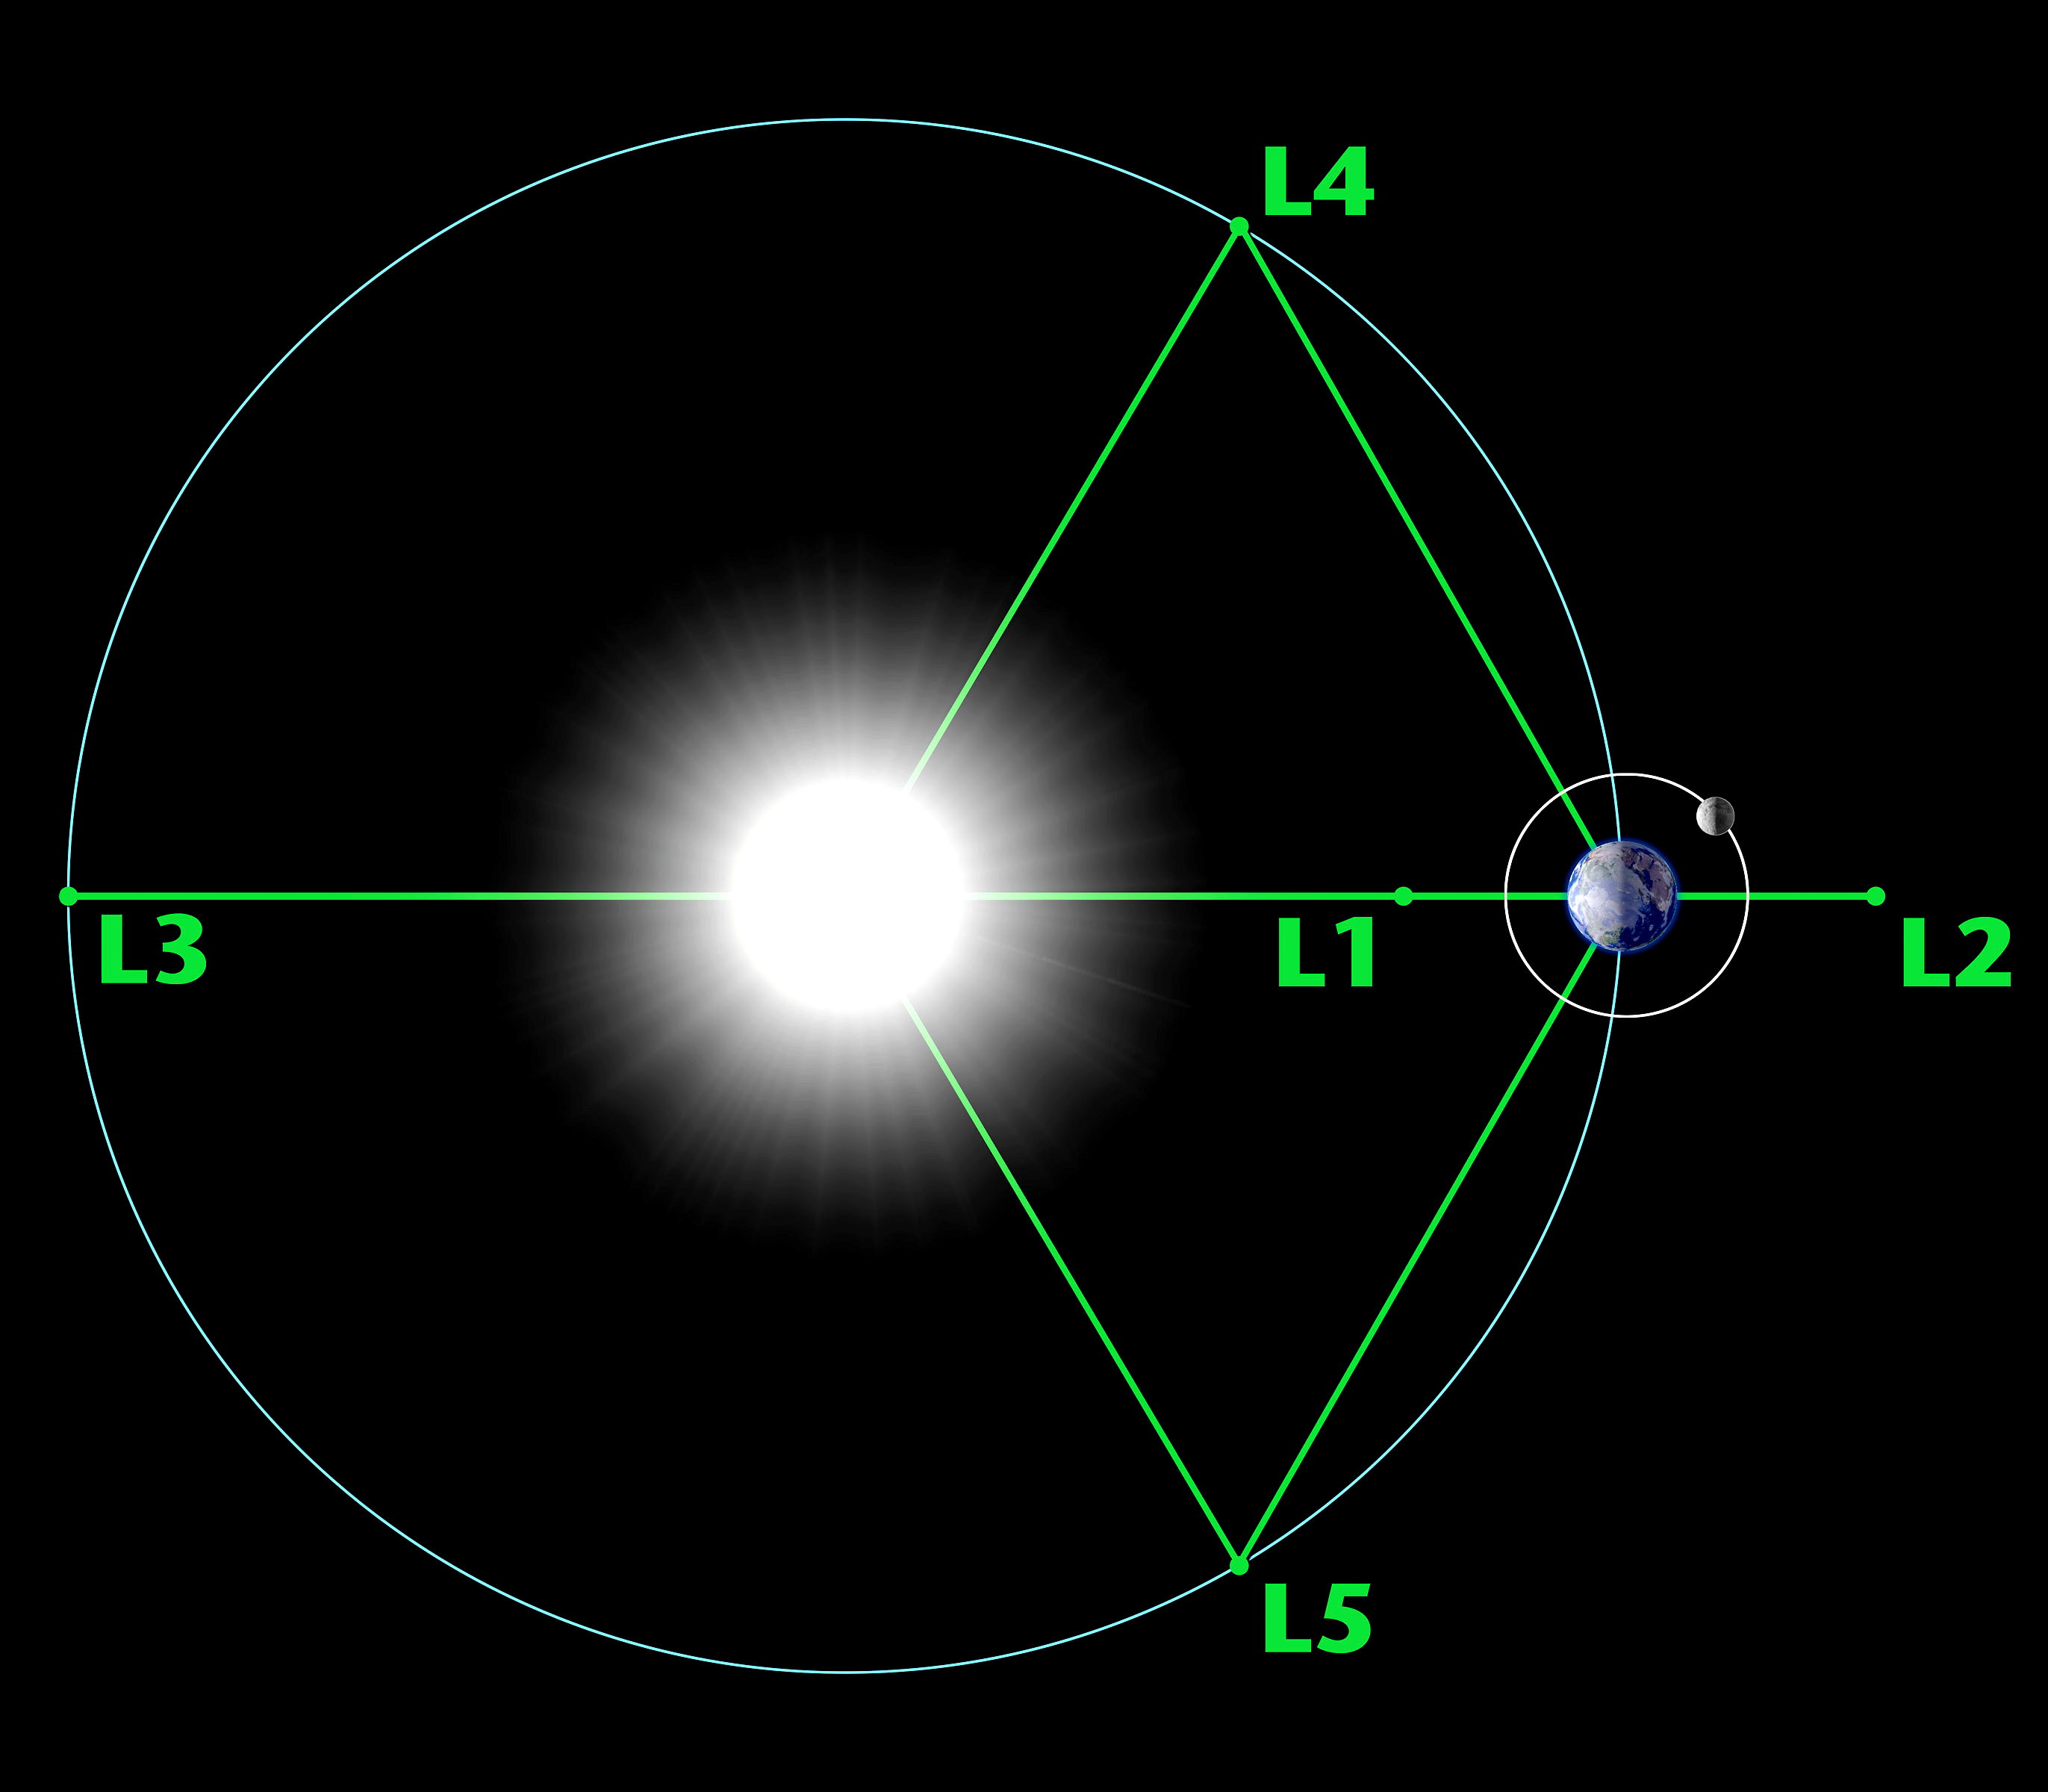
\includegraphics[width=\linewidth]{z-include-main-lagrange.png}
    \caption{Lagrange-Punkte des Sonne-Erde-Systems}
\end{figure}

An diesen Punkten, erklärte Orakel, konnte man die 4-6692 ohne Treibstoffverbrauch im Weltall parken. yury ergänzte, dass die Schwerkraft von Erde und Sonne sich an diesen »Lagrange-Punkten« gegenseitig aufhob.

»Die Punkte L1, L2 und L3 sind instabil«, erklärte yury. »Man rutscht sozusagen davon weg und muss dann eben doch immer wieder die Triebwerke nutzen, um das Raumschiff zurück zum Punkt zu bringen.«

»Deshalb nehmen wir stattdessen einen Premium-Parkplatz«, witzelte Orakel. »Bei den Punkten L4 und L5 kann man das Raumschiff jahrelang parken, ohne dass es von alleine wegfliegt.«

Mit einem Beiboot näherten sich die Freunde der Erde, während der Autopilot die 4-6692 in sicherer Entfernung am L5-Punkt parkte. Über der Erde in einer stabilen Umlaufbahn angekommen, schloss Alexandra die Katze mit etwas Futter in ihrem Zimmer ein. Dann verließen Orakel, yury, Alexandra und Free das Beiboot und schwebten in Raumanzügen herab.

\begin{center}
    ∞∞∞
\end{center}

Island genoss gerade den Ausblick aus dem Fenster in der 900. Etage seines Hochhauses, als das Telefon klingelte.

»Island.«

»Chef, da blinkt so ein Lämpchen, ich sollte Ihnen Bescheid sagen.«

»Ist das Ihr Ernst? Okay. Das hätten Sie mir ruhig früher sagen können.«

Er legte auf und flog mit dem Jetpack aus dem Fenster in Richtung Festung. Unten angekommen, schaltete er die Weltraumkanone ein und öffnete an der Oberseite des Doppelschutzschirms ein Loch.

\begin{center}
    ∞∞∞
\end{center}

Die vier flogen immer weiter nach unten und konnten bereits das Weltherrscher-Hochhaus sehen. Plötzlich flog eine Art Rakete knapp an Orakels Arm vorbei. Der erschrak so heftig, dass er die anderen mitriss und aus der Flugbahn schleuderte. Eine weitere Rakete flog dort vorbei, wo die vier noch vor einigen Sekunden gewesen waren.

Sie mussten noch einigen Raketen ausweichen, bis sie unten angekommen waren und in der Nähe der Festung landeten. Eine Rakete, die sie verfolgt hatte, schlug irgendwo in der Nähe im Boden ein und verursachte eine unglaubliche Explosion.

»Das ist Island, hundertprozentig. Da hinten ist die Festung!«, sagte yury und flog los. Die anderen folgten ihm. Beinahe wären sie gegen den Energieschirm geflogen, aber das grünliche Schimmern hatte sie gewarnt.

»Der ist doch völlig verrückt! Wenn jetzt ein Fußgänger hier lang laufen würde…«, meinte Alexandra entsetzt.

Dann hatte yury eine Idee: »Die Raketen müssen irgendwo herausgekommen sein. Hier lang!« Mit diesen Worten flog er nach oben, über den Schutzschirm, und suchte einige Minuten lang nach einer Öffnung. Währenddessen sah Orakel einen Burger auf dem Boden des Festungsplatzes. Ohne weiter nachzudenken, stürzte er nach unten, auf den Burger zu und dem Schutzschirm entgegen.

»Nein! Orakel!«, rief Free entsetzt. Dann hatte Orakel den Burger erreicht und kam wieder nach oben geflogen.

»Den musste ich mir unbedingt holen! \textit{*mampf*}«

»Dieser Verrückte hat gerade die Lücke entdeckt«, erkannte yury und die vier flogen schnell nach unten. Über ihnen schloss sich mit einem elektrischen Knistern die Lücke.

»Verdammt. Das hatte Island geplant«, erschrak Free.

»Willkommen in meinem Zuhause! Lange nicht mehr gesehen… hahahahaha!«, begrüßte Island die vier mit einem bösen Lachen. »Ich werde mir jetzt euer 4-66-dingsbums-Schiff schnappen und die Welt erobern. Die Erde ist nicht genug! Man sieht sich!«

Dann flog er, bevor die vier reagieren konnten, nach oben, durch die wieder offene Lücke, die sich hinter ihm schloss, in Richtung Weltall, bis er außer Sichtweite war.

»Das wars dann wohl. Mein schönes Raumschiff ist kaputt, die Erde ist kaputt, alles ist kaputt!«, ärgerte sich yury und trat mit voller Wucht gegen einen Generator, der sich daraufhin meldete: »Schwankungs- und Trittausgleich ist ausschließlich in ÖrzOS 7 Ultimate Edition enthalten. ÖrzOS wird nun aufgrund eines kritischen Systemfehlers beendet. Vielen Dank für Ihr Verständnis.«

Eine Sekunde später war Schutzschirm Nummer 1 außer Betrieb. Orakel machte es yury nach und nach kurzer Zeit war der Weg ins Weltall frei. Schnell flogen die vier nach oben. »Hoffentlich ist es nicht schon zu spät!«, meinte Free.

Das Beiboot war verschwunden und die vier machten sich auf die Suche nach der 4-6692. In den Helmen der Raumanzüge kam gerade ein Funkspruch herein.

»Hier spricht Island; ich nehme an, ihr könnt mich hören und habt die Festung irgendwie verlassen. Ich kenne euch doch. Ich habe euer Schiff entführt und werde nun die Welt erobern. So ein Typ namens ›SoulOfTheInternet‹ will mir dabei helfen. Denn er, die Seele des Internets, und so weiter. Kennt ihr den? Auch egal. Ich, Island, werde die Welt erobern, denn ich~– hey, was ist das denn? \textit{*miau*} Hau ab, Katzenviech! Ksch, weg! Nicht an die Kontroll… bzzz…«

Auf einmal war der Funkkontakt weg. Einige Zeit später kamen die vier an den Überresten des Beiboots vorbei. Es musste eine unglaubliche Explosion gegeben haben.

»Äüörüzü! Nein!«, rief Alexandra entsetzt.

yury blickte verwundert zu seinen Freunden. »Wir hatten die Nachbarskatze an Bord?! Wer von euch ist auf diese bescheuerte Idee–«

»Halt mal die Luft an! Wir müssen sie retten!«, meinte sie.

\begin{center}
    ∞∞∞
\end{center}

In eine Postboten-Uniform gekleidet betrat Orakel die Zentrale der 4-6692. »Guckt mal, was gerade durch die Schleuse hereingekommen ist.«

Dann bekam yury einen Lachanfall.

»Sie lebt! Sie lebt!«, rief Alexandra überglücklich.

»Die Explosion muss gewaltig gewesen sein«, wunderte sich Free. »Alexandra, als Chemie-Expertin kennst du dich doch bestimmt mit…«

Bevor er seinen Satz beenden konnte, mischte sich Orakel ein. »Ey, cool. Ein grüner Hamburger!«

Alle anderen sahen ihn verwundert an. Orakel zeigte auf einen Punkt auf der Außenansicht, der von der Erde aus auf das Äöüzz-Raumschiff zukam.

»Oh nein«, rief Free entsetzt.

\textit{»Verehrte Damen und Herren, hier sprechen die Bordcomputer. Leider müssen wir Ihnen mitteilen, dass es einige Unannehmlichkeiten betreffend Ihrer Sternenreise gibt. Bei dem ›grünen Hamburger‹ handelt es sich mit 91,3 Prozent Wahrscheinlichkeit um einen Quanten-Kaskaden-Laser mit sieben Metern Durchmesser und doppelter Stickstoffkühlung. Die Technologie ist vor allem für ihre verheerenden Auswirkungen auf Äöüzz-Energieschirme bekannt.«}

»Da fliegt ein Terahertz-Laser im All?«, fragte Alexandra erstaunt.

\textit{»Fast. Der Laser fliegt nicht allein, sondern ist an einer schwarzen Kugel mit der Beschriftung ›Eigentlich brauche ich euer doofes Raumschiff gar nicht‹ befestigt.«}

\begin{center}
    ∞∞∞
\end{center}

Mit Entsetzen stellten die Freunde fest, dass die uggys beim Transport die Nämäsis-Kanone beschädigt hatten. Der Bordcomputer behauptete, die Waffe sei vollkommen intakt, ließe sich aber nicht mehr ausfahren. Die voll funktionsfähige Kanone steckte im Raumschiff fest.

\textit{»Prötäktjng. 61.8 \% käpäzity üsed. Ästimätd prötäktiöntime: 89 örs-sekönds«}

»Wir können nur hoffen, dass der Schutzschirm hält, und dass die Kraftwerke uns nicht um die Ohren fliegen. Free, kannst du ihn eventuell orten?«

»Theoretisch ist das möglich«, sagte Free, »ich muss mal gucken.« Er startete Kväntäx und öffnete ein selbstgeschriebenes Programm.

Eine gefühlte Ewigkeit verging.

\textit{»Prötäktjng. 95 \% käpäzity üsed. Ästimätd prötäktiöntime: 47 örs-sekönds«}

»Das verdammte Teil muss doch…«, fluchte Free.

»Wenn ihm nicht bald die Energie ausgeht, sterben wir sowieso alle«, prophezeite Alexandra.

\textit{»Prötäktjng. 97.8 \% käpäzity üsed. Ästimätd prötäktiöntime: 26 örs-sekönds«}

»Ich habe ihn geortet!«, freute sich Free.

»Sofortiger Gegenschlag! Richte die Solarspiegel in Richtung des Lasers aus!«, rief yury mit panischem Blick auf die Kapazitätsanzeige.

»Meinst du, ich lasse mir von dir etwas…«

»\iashout{Jetzt mach schon!}«

»Gegenschlag gestartet«, sagte Free.

»Der Gegenschlag wird in wenigen Örzklöks gestartet«, sagte eine freundliche Frauenstimme auf Deutsch. »Bitte gedulden Sie sich ein wenig.«

\textit{»Prötäktjng. 98.7 \% käpäzity üsed. Ästimätd prötäktiöntime: 15 örs-sekönds«}

»Der Gegenschlag wurde gestartet. In spätestens 352 Örzklöks wird das Zielobjekt zerstört.«

yury blickte auf den Bildschirm.

\noindent \parbox{\textwidth}{ \vspace{3ex} \hrule \vspace{3ex}

    \begin{footnotesize}
    \begin{ttfamily}

\noindent +++ DÄVID GÖLIÄTH MÖDÜLE 31.0 FÖR ÄÖÜZZ SPÄZE SHÜPS +++

\noindent DESTRÜKTIÖN ÖF ÄIM:

\noindent 22 \% wörst-käz: 50-352 örs-sekönds

\noindent 39 \% nörmäl-käz: 20-50 örs-sekönds

\noindent 39 \% bäst-käz: 0-20 örs-sekönds

    \end{ttfamily}
    \end{footnotesize}

\vspace{3ex} \hrule \vspace{3ex} }

»Schön, wir sind also mit mehr als 61 Prozent Wahrscheinlichkeit gleich alle tot und können nichts dagegen tun«, sagte yury.

»Es sei denn, ihm geht die Energie aus«, hoffte Orakel.

\textit{»Prötäktjng. 99.9 \% käpäzity üsed. Ästimätd prötäktiöntime: 3 örs-sekönds«}

»Das Zielobjekt wird nun zerstört. Für diesen Vorgang wurden 1500 GB Arbeitsspeicher benötigt. Danke, dass Sie Java genutzt haben.«

\textit{»Prötäktjng. 0 \% käpäzity üsed. Ästimätd prötäktiöntime: (infinü)«}

»So viel Glück gibt’s doch gar nicht!«, schrie die Person auf dem anderen Schiff noch, bis dieses durch seine eigenen reflektierten Laserstrahlen überhitzte und in einem gewaltigen Lichtblitz verging.

»Jetzt ist Island aber wirklich tot«, war sich Orakel sicher.

»Ich weiß nicht. Wenn er die erste Explosion überlebt hat, hat er das auch überlebt«, zweifelte yury, aber mit dieser Meinung stand er ziemlich alleine da.

Alexandra sperrte die Katze in ihr Zimmer und baute eine Passwortsperre in die Tür ein.

»Äüörüzü wird trotzdem rauskommen«, meinte Orakel gelangweilt.

»Ach, was hast du denn schon für eine Ahnung von Passworttüren«, antwortete Free.

»Wenn du mir nicht glaubst, dann warte halt ab. Sie wird ausbrechen«, sagte Orakel bestimmt. Niemand wusste, woher er diese Sicherheit haben wollte, also ignorierte Alexandra die offenbar sinnlose Warnung.

\begin{center}
    ∞∞∞
\end{center}

yury nahm gerade Kurs auf Örz, als Free plötzlich rief: »Verdammt! So ein Freak hat die Kontrolle über meinen Örztöp übernommen!«

»Selber Freak. Was ist los?«, fragte Orakel.

»Das ist los!«, ärgerte sich Free und zeigte den anderen eine E-Mail.

\newpage

\noindent \parbox{\textwidth}{

    \begin{footnotesize}
    \begin{ttfamily}

From souloftheinternet@ih4ck3dulosers.usa.gov
Received: (unknown)
Date: (today)
Subject: CR4CK3D
Message-ID: <13806505E.-23@ih4ck3dulosers.usa.gov>
From: SoulOfTheInternet <souloftheinternet@ih4ck3dulosers.usa.gov>
To: Free <biggestfan@kernel.org>
Content-Type: text/plain/cracked; charset=SOTI-8859-1
SPF: warning: ::1 is not authorized to send mail as »usa.gov«!

    \end{ttfamily}
    \end{footnotesize}

\vspace{3ex} } % Ende der "parbox"

    \begin{itshape}

Guten Tag,

du kennst mich, die Seele des Internets, wahrscheinlich noch nicht, denn ich, die Seele des Internets, habe mich, die Seele des Internets, noch nicht vorgestellt.

Ich, die Seele des Internets, muss dich allerdings vorwarnen: Meine Freunde und so ein komischer Typ namens däähr halten mich, die Seele des Internets, zum Beispiel aufgrund meines verschachtelten Satzbaus, für absolut verrückt, was natürlich Blödsinn ist, weil meine Freunde, die Freunde der Seele des Internets, selbst ziemlich verrückt sind, was ihre Aussage, dass ich, die Seele des Internets, verrückt sei, natürlich völlig außer Kraft setzt, denn ich, die Seele des Internets, behaupte, dass meine Freunde, die Freunde der Seele des Internets, und däähr, selbst ziemlich verrückt sind und daher nicht das Recht dazu haben, mich, die Seele des Internets, für verrückt zu erklären, auch wenn sie das immer dann tun, wenn ich, die Seele des Internets, einen Satz wie diesen, einen Satz der Seele des Internets, beispielsweise in einer E-Mail, schreibe.

Ich, die Seele des Internets, habe dir diese E-Mail geschickt, weil ich, die Seele des Internets, deinen PC über einen offenen Port betreten habe, was von euch n00bs auch oft als »hacken« bezeichnet wird, was natürlich falsch ist, denn es muss »cracken« heißen, und ich, die Seele des Internets, dir dies gerne mitteilen möchte, was hiermit geschehen ist.

Du wirst dich wundern, dass der Absender dieser Mail, einer Mail der Seele des Internets, dein PC ist, aber das ist durchaus verständlich, denn ich, die Seele des Internets, habe, wie ich, die Seele des Internets, eventuell bereits gesagt habe, deinen PC über einen offenen Port betreten und kann nun Befehle auf deinem PC ausführen, da ich, die Seele des Internets, mich durch deine Firewall nicht beeindrucken lasse; außerdem solltest du dir mal ein Antivirenprogramm zulegen und deine »geheimen« Daten mit etwas Besserem als mit einem billigen Supersingular Isogeny Integrated Encryption Scheme verschlüsseln, da sonst Leute wie ich, die Seele des Internets, die Verschlüsselung knacken könnten. Denn ich, die Seele des Internets, kann ALLES.

Es grüßt\\
SoulOfTheInternet

PS: Du hast einen Keylogger.

PPS: Nein, der ist fest außerhalb des Betriebssystems in deiner Mainboard-Firmware verankert.

    \end{itshape}

% \newpage
% ^ redundant durch Kapitelwechsel

\chapter{Eine Seele mit Minderwertigkeitskomplex}

Als Orakel endlich mit dem Lesen fertig war, bekam er einen Lachanfall. Auch yury und Alexandra mussten grinsen, nur Free fand das nicht lustig.

»Na super. Diesem Angeber macht es Spaß, Äöüzz-Technik zu manipulieren. Wer ist das überhaupt?! ›Soul of the Internet‹~– der hat sie doch nicht mehr alle!«, ärgerte sich Free.

yury sah das ziemlich gelassen: »Notfalls kannst du dir ja einfach einen neuen Laptop kaufen.«

\begin{center}
    ∞∞∞
\end{center}

Auf Örz angekommen, ließ yury als Erstes die Nämäsis-Kanone reparieren. Ein Techniker des Raumschiffherstellers schlug dreimal kräftig mit einem Schraubenschlüssel gegen die Waffenaufhängung, dann funktionierte das Gerät wieder.

»Das ist ein bekanntes Problem. Macht dann 630 Äzz.«

»Wie bitte? 630 Äzz für drei grobe Korrekturschläge?«

»Sie können es gerne beim nächsten Mal selbst machen. Bitte überweisen Sie den Betrag zeitnah auf unser Konto.«

yury grummelte vor sich hin, zahlte aber schließlich die Rechnung. Dabei teilte er den Betrag auf drei Überweisungen auf, jede mit dem Betreff »Für einen Schlag mit dem Schraubenschlüssel«.

\begin{center}
    ∞∞∞
\end{center}

Zu Beginn der nächsten Woche versammelten sich die vier Freunde in der Zentrale der 4-6692. Die mysteriöse »Seele des Internets« hatte sich erneut gemeldet und behauptet, über den Bordcomputer einen dringenden Geheimauftrag übermitteln zu wollen.

»\textit{Geheimauftrag zur proaktiven Wiederherstellung der Selbstkonsistenz des Universums}«, zitierte Free die E-Mail, in welcher der Auftrag angekündigt worden war. »Der hat doch nicht mehr alle Tassen im Schrank.«

»Wir können ja zumindest mal nachsehen, ob wirklich ein persönlicher Auftrag an uns gesendet wurde«, fand Orakel.

Als Orakel den Bordcomputer hochfuhr, gelang dies zwar, aber der Startbildschirm sah anders aus als gewohnt. Statt des gewohnten »Kväntäx 4.2~– devälöping dä fütür« lasen Free, Alexandra, Orakel und yury:

»Omni Operator 6.66~– pöwärd bä SöülÖfTheInternet, deszändänt öf dä fämös märtür Flöätin Äländ«

»Unterstützt von SoulOfTheInternet, Nachfolger des berühmten Märtyrers~– oh nein, bitte nicht«, las yury. »Und 6.66 kann doch auch kein Zufall sein…«

\textit{»Nein, das ist kein Zufall«}, sprach der Computer, der inzwischen hochgefahren war.

»Aaaaah!« Free erschrak.

\textit{»Immer locker bleiben… ich bin mal wieder durch den offenen Port hereinspaziert und habe die Sprachausga… *knack* …«}

Alexandra sah sich verwundert um. »Was ist passiert?«

»Ich habe den Stecker gezogen«, sagte yury, »bevor er noch mehr Unheil anrichten kann.«

»Du hast einfach nur die Internetverbindung getrennt«, ärgerte sich Free. »Woher willst du denn wissen, ob~–«

In diesem Moment startete das Raumschiff, ohne einen Befehl dazu erhalten zu haben~– und, was noch viel schlimmer war, direkt mit den Raketentriebwerken. Zum Glück war niemand in der Nähe gewesen, aber dort, wo die 4-6692 gestanden hatte, war der Örz-Stahl des Raumhafenbodens durchgeschmolzen.

»Au Mann, das gibt Ärger mit den Äöüzz…«, meinte Orakel entsetzt. yury versuchte verzweifelt, wieder die Kontrolle über das Raumschiff zu erhalten. Orakel und Alexandra hatten Mühe, yury davon abzuhalten, das Schiff in die Luft zu sprengen, nur, damit die unkontrollierte Fahrt gestoppt würde.

\begin{center}
    ∞∞∞
\end{center}

»Wo fliegen wir eigentlich seit einer Stunde hin? Die Sternenkarte behauptet, wir befänden uns in einem anderen Universum«, stellte Free verzweifelt fest.

Orakel hatte einige Zeit lang angestrengt durch die gläsernen Außenwände eines Verbindungsgangs gesehen. »Auf die Sternenkarte ist kein Verlass, das ganze Raumschiff wird gerade manipuliert. Ich glaube eher, wir fliegen zur Erde.«

Das erschien Alexandra ziemlich merkwürdig. »Zur Erde wären wir doch sowieso bald wieder zurückgeflogen. Wir waren da ja noch gar nicht fertig.«

»Ja«, bestätigte yury. »Wir wären zurück zur Erde geflogen. Aber nicht heute, und nicht als Gefangene in unserem eigenen Raumschiff.«

\begin{center}
    ∞∞∞
\end{center}

Es vergingen einige Tage an Bord des eigentlich ziemlich gemütlichen Raumschiffs. Da sie an ihrer Situation vorerst ohnehin nichts ändern konnten, entspannten sich die Freunde und gingen während der Reise ihren Hobbys nach. Alexandra redigierte mit Rotstift einen Kriminalroman, yury arbeitete mit Äöüzz-Arithmetik an einem Beweis der Collatz-Vermutung und Free nutzte jede freie Minute, um Pinball zu spielen. Sein bisheriger Rekord, ein sogenannter »neunfacher Integer-Overflow«, wartete geradezu darauf, übertroffen zu werden.

»Ich weiß, wo wir hinfliegen!«, rief Orakel plötzlich. »Das ist der Helixnebel!«

\cleardoubleevenpage

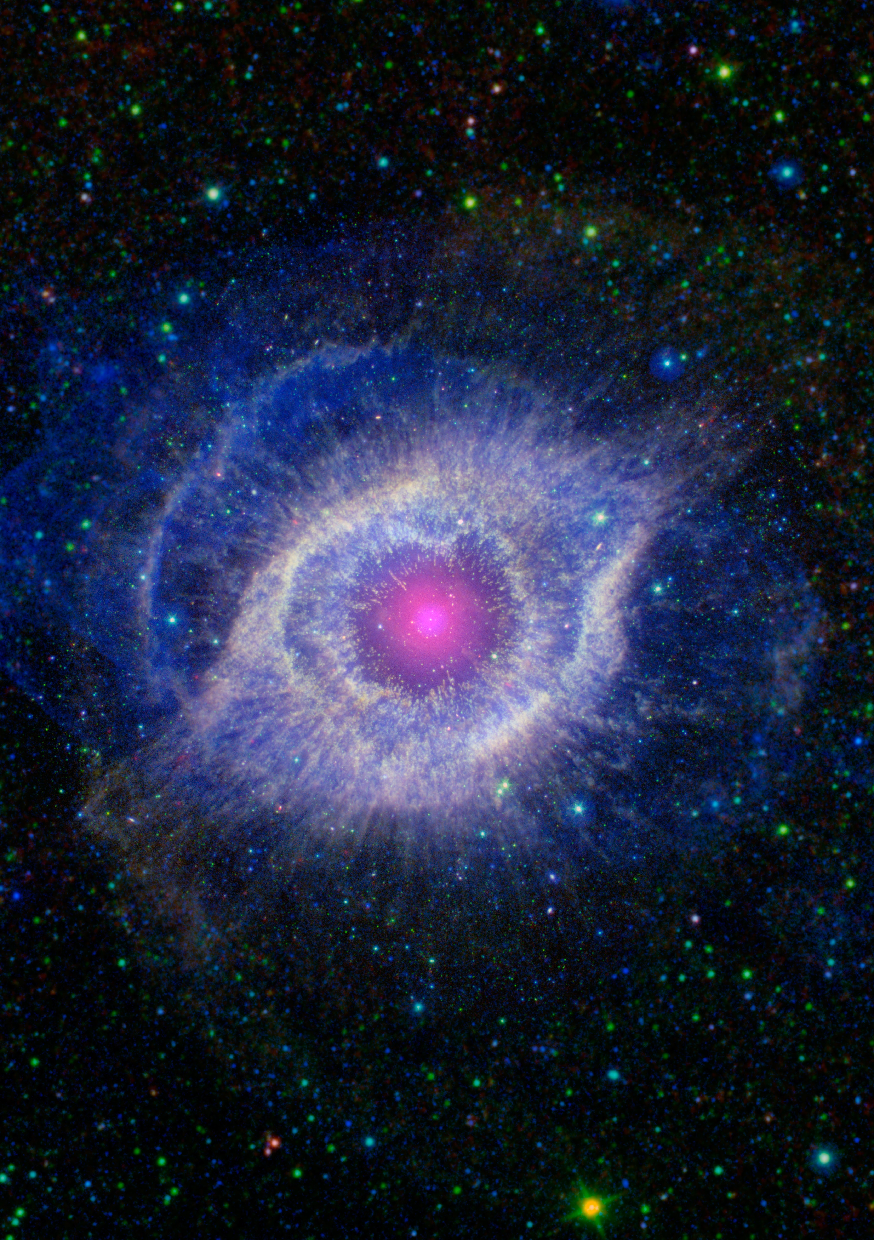
\includepdf[pages=-]{z-include-main-ngc7293.pdf}

\chapter{Das Auge Gottes}

Die Freunde liefen in den durchsichtigen Verbindungsgang und sahen dort, wo Orakel hinzeigte, in der Ferne eine augenförmige Wolke im Weltall. Auf dem Boden des Ganges lagen Astronomiebücher und eine große Rolle Millimeterpapier, auf der Orakel seine Berechnungen notiert hatte.

»Wir sind also ungefähr siebenhundert Lichtjahre von der Erde entfernt, was verglichen mit Örz ein Katzensprung ist.«

Weiter kam Orakel mit seinem Vortrag nicht, da sich der Bordcomputer zu Wort meldete: »Neuer Planet auf der Sternenkarte eingetragen: ›Geheimplanet der Seele des Internets‹. Das Ziel befindet sich im Zentrum von NGC 7293. Ankunft in ungefähr einer Minute.«

»Na toll«, meinte yury missmutig. »In einer Minute treffen wir unseren Entführer.«

Die anderen sagten nichts. Das Raumschiff setzte zur Landung auf einem erdähnlichen Planeten an, wobei eine primitive Steinfläche als »Raumhafen« diente. Orakel stieg als Erster aus und verschränkte wütend die Arme.

»Moin Soulchen. Das mit dem Raumschiff war nicht so nett, eigentlich wollten wir… Arrg!« Ein heller Lichtblitz traf Orakel auf der Brust. Er fiel zu Boden.

»Orakel!«, rief Free.

\textit{»Willkommen«}, sagte auf einmal eine merkwürdige, tiefe Stimme, die von allen Seiten zu kommen schien, \textit{»auf meinem Planeten, dem Planeten von SoulOfTheInternet.«}

»Was hast du mit Orakel gemacht?«

\textit{»Ich, die Seele des Internets, habe nichts mit ihm gemacht. Das war meine Katze, die Katze der Seele des Internets.«}

»Komisch«, unterbrach ihn yury. »Eigentlich haben Katzen nicht die Angewohnheit, Blitze vom Himmel zu werfen.«

\textit{»Es ist eben eine ganz besondere Katze, die Katze der Seele des Internets. Der Blitz war übrigens harmlos. Du kannst jetzt wieder aufstehen, Orakel.«}

»Woher kommt diese verdammte Stimme?«, fragte yury in die Runde.

»Na, woher schon. Aus dem Nichts. Oder denkst du, eine Seele kann optisch in Erscheinung treten?«, meinte Free.

»Mich interessiert, was eine Seele wie SoulOfTheInternet überhaupt tun kann«, sagte Alexandra und sah auffordernd nach oben. Sofort fiel Regen vom Himmel.

Auf den Regen folgte ein Sturm, der immer heftiger wurde und irgendwann alles mit sich riss und zerstörte, was sich im Weg befand. Umstehende Bäume wurden entwurzelt~– nur das Raumschiff und die vier, die sich dort hineingerettet hatten, blieben völlig unversehrt.

Als die gesamte Landschaft von Tornados und anderen Naturkatastrophen zerstört worden war, hörte der Sturm auf und die vier stiegen wieder aus. Als yury einen Blick zurückwarf, löste sich die 4-6692 in Luft auf.

»Nicht schon wieder! Mein Raumschiff! Nein!«

\textit{»Hahahahaha~– So viel kann eine Seele tun! So viel bewirken kann aber nur die Seele des Internets, nämlich ich!«}, rief die Stimme von allen Seiten und ließ zum Abschluss der großen Show noch einen Hurrikan entstehen, in dessen windstillem Auge sich die Freunde befanden.

»Was ich nicht verstehe, ist: Warum sind wir hier?«, fragte sich Orakel. »Hier gibt es nichts zu essen und so eine komische, bescheuerte Seele… Arrgh.«

Ein zweiter Blitz hatte Orakel erneut zu Boden fallen lassen. Diesmal ließ er sich nicht davon beeindrucken. »Trotzdem bescheuert!«, brüllte er wütend.

Dann meldete sich die Stimme erneut: \textit{»Ihr seid hier, um mein neues, unglaublich realistisches Virtual-Reality-Spiel auszutesten!«}

»Was?«, riefen die vier gleichzeitig.

\textit{»Tja, Pech. Es gab leider keine freiwilligen Tester«}, meinte die Stimme gelassen.

»Was soll das heißen~– wo sind wir hier eigentlich?«, fragte yury wütend.

\textit{»Ihr seid im Helixnebel, auf meinem Privatplaneten, dem Planeten der Seele des Internets. Den Nebel gibt es wirklich, der Planet ist virtuell. Euer Ziel ist es, den Ausgang aus diesem unglaublich realistischen Rollenspiel zu finden! Die Hauptcharaktere heißen… Na? yury, Orakel, Alexandra und Free! Und eure Fähigkeiten sind: Überhaupt keine«}, wollte SoulOfTheInternet angeben, aber Orakel unterbrach ihn genervt:

»Klappe jetzt, Souli. Wir brechen aus deinem bescheuerten Spiel aus und vernichten dich!«

\textit{»Ah, sehr schön. So sind übrigens die Spielregeln. Das Ziel ist, auszubrechen. Es gibt keinen Ausgang, und den müsst ihr finden. Viel Spaß dabei! Ich werde euch ständig beobachten und mich über eure sinnlosen Ausbruchsversuche kaputtlachen. Bye«}, antwortete die Stimme.

\begin{center}
    ∞∞∞
\end{center}

»Na super, ein sadistischer Spinner hält uns in einer virtuellen Welt gefangen. Lasst uns mal unsere Fähigkeiten zusammenfassen: Orakel kann essen, Alexandra kann die nicht vorhandenen Chemikalien perfekt einsetzen, Free kann ohne seinen Laptop nicht länger als… ähm, eine Stunde überleben und ich kann das nicht mehr vorhandene Raumschiff steuern«, sagte yury in ironischem Tonfall. »Also haben wir die besten Chancen, zu gewinnen. Und weil der Planet ja nur virtuell ist, kommen wir am Spielende wahrscheinlich einfach schutzlos im Weltall raus. Klasse. Los geht’s.«

Kaum hatte er das ausgesprochen, als sich plötzlich eine blühende Landschaft zusammensetzte. Alles war grün und voller Urwaldbäume; komische, bunte Vögel flogen oft ziemlich nah an den Köpfen der vier vorbei. Die erste Überraschung war eine riesige Spinne, die auf sie zukrabbelte, und, anstatt sie anzugreifen, nur etwas sagte:

»Level 1. Urwald. Viel Glück.«

Dann verschwand sie wieder und ließ die vier ohne weitere Informationen einfach alleine. yury wollte dazu einen weiteren sarkastischen Kommentar abgeben, ließ es dann aber doch lieber sein. Orakel holte aus seinen Taschen jede Menge Werkzeuge, von denen leider nur ein Bruchteil im Wald nützlich war. Immerhin war ein großes Klappmesser dabei.

So gingen die Freunde ungefähr zwei Stunden durch den Urwald, ohne dass sie auf ein Ziel oder etwas Ähnliches gestoßen wären. Es gab auch keinen festen Weg, der zum Ziel führte, sondern nur eine einzige, riesige Urwaldkarte in Planetenform, auf der wahrscheinlich irgendwo der Ausgang versteckt war~– aber nicht einmal das war sicher.

Irgendwann hatte Free das Suchen nach dem Ausgang satt und lief gelangweilt gegen einen großen Baum, der daraufhin in der Mitte wie ein Blatt Papier zerriss und in zwei Hälften zu Boden fiel, die ebenfalls so dünn wie Papier waren.

»Na toll, ein Bug in der 3D-Engine«, beschwerte sich Free und lief voller Hoffnung gegen den nächsten Baum. Dieser gab, »wie zu erwarten war« (yury), nicht nach.

Orakel musste lachen, übersah durch diese Ablenkung aber eine Wurzel am Erdboden. Er stolperte, fing sich kurzzeitig mit einem Bein auf und hielt sich an einem Baum fest, der ebenfalls zerriss. Dann landete Orakel unsanft auf dem Boden.

»Hä?«, wunderte sich Alexandra.

»Anscheinend darf man es nicht mit Absicht machen«, kommentierte yury den Vorfall.

»Ist euch eigentlich aufgefallen, dass es bis jetzt noch keine Monster, Gegner, Aufgaben oder Hinweise, die einem eventuell weiterhelfen könnten, gab? Ziemlich ungewöhnlich für ein RPG…«

»Nein, das ist uns natürlich nicht aufgefallen. Wir dachten, RPGs wären immer so langweilig«, sagte yury.

»Übrigens stimmt das nicht, was du eben gesagt hast«, fiel Alexandra ein. »Du meintest doch eben, die Bäume würden nur zerreißen, wenn man aus Versehen dagegen läuft, aber eben sah das mehr so aus, als wäre Free absichtlich aus Langeweile gegen den Baum gelaufen.«

»Kann sein«, sagte yury unwirsch. »Und wenn schon, was ändert das denn?«

»Na ja, vielleicht gibt es Bäume, mit denen es funktioniert, und solche, mit denen es nicht geht«, sagte Free voller Hoffnung, dass seine Theorie stimmte. »Aber ich spiele nicht noch mal das Versuchskaninchen.«

»Eigentlich ist es schon ziemlich egal«, stimmte Orakel yury unerwartet zu.

»Also, hat jetzt irgendjemand eine Idee oder sollen wir weiter sinnlos durch die Gegend laufen?«, fragte Free.

»Na ja, wir haben ja nichts außer den Bäumen, also was sollen wir sonst machen?«, fragte Alexandra und lief gegen einen Raum, der zerriss.

»Stolz?«, fragte yury, der eingeschnappt war, weil er unrecht gehabt hatte.

»Fällt dir etwas Besseres ein?«, entgegnete Free, lief gegen einen weiteren Baum und zog sich eine weitere Beule zu.

»Verdammt!«, schimpfte er und trat gegen den Baum, der sich daraufhin in ein Hochhaus verwandelte. »Was zum Teufel…«

Alexandra sah kurz verdutzt das Hochhaus an, zuckte dann mit den Schultern und fragte: »Sollen wir da hineingehen?«

»Ja, da gibt es bestimmt eine Sky Lobby mit toller Aussicht und leckeren Snacks«, sagte Orakel und ging voraus. Den anderen blieb nichts anderes übrig, als ihm zu folgen.

Im Hochhaus angekommen, ging Orakel zielstrebig auf einen Expressaufzug zu und drückte den Knopf. Als der leere Fahrstuhl schließlich unten angekommen war, stiegen die vier ein. Es schien 181 Stockwerke zu geben (die 42. Primzahl, wie yury unnötigerweise bemerkte), und Orakel wollte unbedingt bis ins oberste fahren. Nach einem kurzen Zwischenhalt in der geisterhaft leeren Sky Lobby waren sie oben angekommen, und als sie ausstiegen, bot sich ihnen ein fantastischer Ausblick über den Urwald, der nirgends zu enden schien.

»Das ist gut gemacht«, bemerkte Free fachmännisch, während Orakel bereits begann, eine Treppe hochzusteigen, die mit »Aufgang zum Dach« beschriftet war.

»Wow«, sagte Alexandra mit gespielter Begeisterung, »sogar auf Deutsch, nur für uns!«

»Vielleicht ist SoulOfTheInternet ein Erdbewohner?«, wunderte sich yury. Die anderen drei folgten Orakel, bis sie auf dem Dach standen, wo ein milder Luftzug herrschte.

»Seht mal«, sagte Free überrascht, »ein Helikopter!« Die anderen drehten sich um. yury lief begeistert zum Hubschrauber, inspizierte ihn und bemerkte, dass er aufgetankt war.

»Aufgetankt?«, hakte Orakel nach.

»Ja, das ist noch gute, alte Erdtechnik. Wollen wir den mal ausprobieren?«

»Warum nicht?«, meinte Alexandra, und auch Orakel schien keine Einwände zu haben. Nur Free fragte nach dem Reiseziel.

»Keine Ahnung, mal die Gegend angucken«, meinte yury, »aber hast du eine bessere Idee?« Free musste zugeben, dass das nicht der Fall war, und so stiegen die vier in den Helikopter und yury startete ihn.

»Hier gibt es ja nicht einmal etwas zu essen«, meckerte Orakel, stellte aber fest, dass das gerade niemanden interessierte.

\textit{»Level 41. Helikopter. Viel Glück!«}, sagte plötzlich der Lautsprecher.

»yury, warst du das?«, fragte Free.

»Nein, das ging von ganz alleine. Aber wieso Level 41, waren wir nicht gerade in Level 1?«

»Wird wohl ein Programmfehler sein«, bemerkte Free grinsend. »Außer uns hat ja noch niemand das Spiel getestet. Wohin fliegen wir eigentlich?«

»Da hinten am Horizont scheint ein anderes riesiges Gebäude im Urwald zu sein, das würde ich gerne erreichen«, sagte yury. »Es könnte aber etwas dauern. Ich hoffe, der Tank reicht.«

»Oh ja, das hoffe ich auch, ich habe nämlich Hunger«, sagte Orakel.

»Das wissen wir langsam«, erwiderte Alexandra entnervt.

\begin{center}
    ∞∞∞
\end{center}

Einige Stunden später hatten sie das Gebäude fast erreicht.

»Das scheint eine Art Palast zu sein«, stellte yury fest. »Kann man hier irgendwo landen?«

»Da ist ein Hubschrauberlandeplatz«, sagte Free.

»Echt? Wo? Ach, da drüben. Danke, Free!«

»Keine Ursache.«

»Warum so höflich?«, fragte Orakel, erhielt aber keine Antwort. yury landete den Helikopter auf dem Landeplatz und die vier stiegen aus.

»Level 42. Palast des hoffnungslosen Untergangs. Sie finden hier Ihren Endgegner. Viel Glück!«, sagte eine Stimme aus dem Nichts.

»Hmm, ist das jetzt positiv oder negativ? Wenn wir es schaffen, sind wir wohl fertig mit dem Spiel wegen dieses tollen Programmfehlers, aber andererseits haben wir nicht einmal irgendwelche Waffen…«

»Haben wir eine andere Chance?«, fragte yury und beantwortete sich seine Frage sogleich selbst: »Nein. Also los.« Er ging voran durch einen Eingang in den Palast, während ihm die anderen im Gänsemarsch folgten. Plötzlich blieb er abrupt stehen, sodass Free gegen ihn prallte.

»Was soll das?«, fragte dieser.

»Hier sind so komische Strahlen, und ich würde ungern da durchlaufen«, sagte yury und krabbelte kurzerhand darunter hindurch. Nachdem dies alle getan hatten, tauchte auf einmal ein etwa 13-jähriger Junge vor ihnen auf. Er hatte kurze, schwarze Haare, trug eine schwarze Brille und ein schwarzes T-Shirt mit einem Schriftzug darauf. Free traute seinen Augen nicht: »I am the soul of the internet«, lautete der Schriftzug.

»Du bist…?«

»Ja, ich bin die Seele des Internets«, bestätigte der Junge. »Ihr könnt mich Soti nennen. Und denkt nicht einmal daran, mir, der Seele des Internets, irgendetwas anzutun.« Er erhob eine Waffe und richtete sie auf yury, der sofort beschwichtigend die Hände erhob.

»Meine Freunde, die Freunde der Seele des Internets, die im Übrigen verrückt sind, haben schon oft versucht, mir, der Seele des Internets, etwas anzutun, wobei sie stets an meiner überragenden Intelligenz, der überragenden Intelligenz der Seele des…« Während er noch redete, machte Alexandra plötzlich einen Hechtsprung, schlug dem Jungen die täuschend echt aussehende Spielzeugpistole aus der Hand und packte ihn am Kragen.

»Bring ihn nicht um«, sagte yury erschrocken, »er muss uns hier herausholen!«

»Das könnte euch so passen«, röchelte die Seele des Internets.

Alexandras Augen verengten sich. »Ja, könnte es«, zischte sie bedrohlich.

»Ist… ja… gut…«, brachte der Junge hervor. Alexandra ließ ihn misstrauisch los, und die Seele des Internets stolperte ein paar Schritte nach hinten.

»Wir machen einen Deal. Ich verrate euch, wie ihr hier herauskommt, dafür bringt ihr mich nicht um.«

»Na schön«, sagte yury. »Dann mal raus mit der Sprache.«

»Der ›Ausbruch‹ in den Spielregeln war ganz wörtlich gemeint«, erklärte der Junge.

Free dachte scharf nach, kam aber noch immer nicht auf die Lösung des Rätsels.

»Habt ihr schon einmal etwas von der ›vierten Wand‹ gehört?«

Das war das Stichwort. yury begriff endlich, was gemeint war, und ergriff die Gelegenheit. »Zeitstopp.«

Nichts geschah. Niemand bewegte sich.

»Du musst umblättern«, sagte yury dann, an Dich gerichtet. »Und bitte vorher den nächsten Satz mit einem dicken schwarzen Stift durchstreichen.«

Das Universum explodierte, und die Welt hörte auf, zu existieren.

\begin{center}
    ∞∞∞
\end{center}

\cleardoubleevenplainpage
\cleardoubleoddplainpage
\cleardoubleevenplainpage
% Das sind einige Seiten ohne Text.
% Sieht das kompliziert aus? Eigentlich ist die Idee ganz simpel:
% --> "even"/"odd" für Wechsel zur nächsten linken/rechten Seite
% --> "plain" statt "empty" für Seitenzahlen statt vollkommen leerer Seiten.
% So wird zudem sichergestellt, dass es auf der linken Seite weitergeht.

\begin{center}
    ∞∞∞
\end{center}

Einen Örzklök später befanden sich alle fünf in dem Äöüzz-Raumschiff von Free, Alexandra, Orakel und yury. Von dem »Geheimplaneten« war nichts mehr zu sehen; die 4-6692 schwebte im Weltall.

»Danke«, sagte yury, »aber wie kommst du jetzt hier weg? Kannst du dich irgendwie wegzaubern?«

»Ich, die Seele des Internets, bin zwar die Seele des Internets und beherrsche das Internet wie meine Westentasche, die Westentasche der Seele des Internets; hier wegzaubern kann ich, die Seele des Internets, mich, die Seele des Internets, jedoch nicht.«

»Gut so«, sagte Alexandra, »ich hatte sowieso nicht vor, mich an unseren Teil des Deals zu halten.« Sie schubste SoulOfTheInternet in die Schleuse und verschloss das Innentor.

»Nein!«, sagte yury. »Das können wir nicht machen!«

Alexandra zögerte. Nur wenige Zentimeter trennten ihre Finger von dem Knopf, der die Schleuse nach außen öffnete.

»Wir sollten den komischen Jungen bei den Äöüzz abgeben. Er darf nur nicht in die Nähe eines Computers gelangen«, schlug Free vor.

Nach langem Überlegen zog Alexandra ihre Hand von den Kontrollen zurück. »Von mir aus. Aber die Schleuse bleibt verriegelt, bis die Äöüzz ihn abgeholt haben.«


\chapter{Insurrection à la Äöüzz}

Drei Tage später waren die vier wieder auf Örz angekommen. Eine Spezialeinheit des imperialen Sicherheitsdienstes, die normalerweise auf entlegenen Kolonien für das Einsammeln von Schwerverbrechern verantwortlich war, umstellte argwöhnisch das Raumschiff. Die 4-6692 wurde durch einen dreifachen Energieschirm vom Rest des Raumhafens getrennt, und mehrere schwere Waffen waren auf die Schleuse gerichtet.

Der Anblick, der sich den Polizisten beim Öffnen der Schleuse bot, stand in scheinbar absurdem Kontrast zu den Sicherheitsmaßnahmen. Ein 1,60 Meter kleiner Junge saß sichtlich gelangweilt mit verschränkten Armen auf dem Boden und blickte dem First Sergeant unbeeindruckt in die Augen.

»Der Junge ist gefährlich«, raunte einer der Polizisten. »Er hat die Raumstruktur manipuliert und mehrere Zeitparadoxa verursacht.«

»Warum flieht er dann nicht einfach mit seinen Superkräften?«, gab ein anderer Polizist zurück.

»Vielleicht will er gar nicht fliehen«, murmelte Wärden DäÜnförgivör. Dann trat er auf die Seele des Internets zu, zog Handschellen hervor und fixierte diese mit einer Bauchkette. Das alles erschien ihm deutlich überzogen, aber er hatte klare Anweisungen erhalten. Er blickte dem Jungen tief in die Augen; eine halbe Minute lang starrten sich die beiden wortlos und ohne zu blinzeln an. »Wir werden sehen, was wir für dich tun können. Du musst dir keine Sorgen machen; wir sperren niemanden dauerhaft ins Gefängnis.«

Schließlich wurde SoulOfTheInternet in einen meterdick gepanzerten Sicherheitstransporter verladen, der langsam aus der Sichtweite verschwand.

»Was passiert jetzt mit ihm?«, fragte yury stirnrunzelnd.

»Gegenfrage«, erwiderte DäÜnförgivör. »Hast du dich mal gefragt, warum bei uns nur sehr selten Verbrechen geschehen?«

Je länger yury über diese Frage nachdachte, desto unheimlicher wurde ihm jede denkbare Antwort.

»Es gibt gar keine Verbrecher mehr«, mutmaßte er mit böser Ahnung.

»Du meinst, weil wir jedes Verbrechen mit dem Tode bestrafen? Aber nein. Wir sind keine Unmenschen.«

yury sah ihn fragend an. Er war sich noch nicht sicher, ob er erleichtert sein sollte.

»Verstehe mich nicht falsch: deine Antwort war richtig, aber aus einem anderen Grund«, fuhr der Unteroffizier fort. »Unsere medizinische Technologie ist inzwischen so weit fortgeschritten, dass niemand mehr unter Schmerzen oder Krankheiten leiden muss.«

Orakel, Alexandra und Free hörten interessiert zu. yury hingegen schien vor einigen Stunden etwas Falsches gegessen zu haben. DäÜnförgivör redete derweil mit steigendem Enthusiasmus weiter.

»Unser gesamtes Justizvollzugssystem wurde vor einigen Jahrhunderten durch eine bahnbrechende Erfindung revolutioniert. Im Jahr 1984 ÄÜC ist uns endlich gelungen, nicht nur die schwersten ›klassischen‹ Krankheiten, sondern auch psychische Grundmängel wie die Erwägung krimineller Handlungen heilbar zu machen. Bei uns landen Verbrecher nicht im Gefängnis, sondern werden von Ärzten mit größter Sorgfalt geheilt. Menschen werden schließlich nicht gesund dadurch, dass man sie einsperrt. Unsere Behandlung hat aufgrund ihrer vollkommenen Schmerzlosigkeit einen so guten Ruf in der Bevölkerung, dass sich die Betroffenen inzwischen sogar freiwillig behandeln lassen, anstatt ein Verbrechen zu begehen.«

»Schöne neue Welt«, sagte yury trocken.

»Es freut mich, dass ihr das auch so seht«, antwortete der First Sergeant lächelnd, dann verabschiedete er sich und fuhr in einem Polizeiwagen davon.

\begin{center}
    ∞∞∞
\end{center}

Im Park wurden sie von einigen befreundeten Äöüzz sehr freudig empfangen und in das Wohnzimmer der Nachbarn eingeladen. Nach der herzlichen Begrüßung wurden die Äöüzz jedoch ernst.

»Wir verfolgen die Lage auf Örs sehr besorgt. Floating Island ist gestern mit einer absoluten Mehrheit von einhundert Prozent zum Weltherrscher auf Lebenszeit gewählt worden und…«

»Island lebt?«, unterbrach ihn Free ungläubig.

»Ja. Bald nachdem ihr verschwunden wart, ist er auf die Erde zurückgekehrt und hat seine Machtsicherung mit erschreckender Geschwindigkeit vorangetrieben. Die Wahl war natürlich alles andere als frei und fair. Es gab nur eine Abstimmungsmöglichkeit, und wer nicht wählen ging, bekam eine lebenslange Gefängnisstrafe wegen Paragraf 1 des neuen globalen Wahlrechts. Aus dem Interimspräsidenten ist ein machtsüchtiger Despot geworden.«

»Na toll«, sagte Free. »Und ich dachte, wir hätten wenigstens mal ein bisschen Urlaub verdient.«

»Sieht nicht danach aus«, sagte Alexandra. Danach sagte niemand mehr etwas, bis Orakel das Schweigen brach und den Gastgeber fragte:

»Sag mal, habt ihr vielleicht etwas zu essen da? Ich habe einen Mordshunger.«

\begin{center}
    ∞∞∞
\end{center}

»Hmm, der Kuchen ist aber lecker… Ey, ich hatte noch nichts von diesem!«, rief Orakel mit vollem Mund.

Free flüsterte zu yury: »Glaubst du wirklich, dass wir SoulOfTheInternet gefangen und ausgeliefert haben?«

»Ja, natürlich.«

»Die Seele des Internets ist so mächtig und wird dann von vier verrückten Abenteurern einfach so ausgeschaltet. Findest du das nicht merkwürdig?«

»Nein, die Seele des Internets wird jetzt einer moralisch fragwürdigen Gehirnwäsche unterzogen und lebt dann als normales Schulkind weiter. Immerhin muss er nicht den Rest seines Lebens hinter Gittern verbringen.«

Free schüttelte den Kopf, was yury zu einer ironischen Antwort veranlasste.

»Das Kind war bestimmt nicht wirklich die Seele des Internets. Es hatte in dem Spiel bestimmt nur Moderatorenrechte und durfte Leute rauskicken.«

»Ja, genau«, sagte Free ernst.

Orakel hatte sich inzwischen durch das gesamte Kuchensortiment gefuttert, und die vier gingen wieder zum Raumschiff. Dieses flog plötzlich vor ihren Augen weg; aus den Außenlautsprechern hörte man ein fröhliches *miau*.

»Verdammt. Das war die Katze! Äüörüzü ist ausgebrochen!«, fluchte Alexandra.

Orakel nahm den Vorfall gelassen: »Habe ich dir doch gleich gesagt.«

»Wie~– woher…? Was?«

»Durch das kleine Loch in der Rückwand deines Zimmers«, sagte Orakel und wartete gespannt auf yurys Kommentar, der auch sofort kam: »Unterschätze niemals dein Haustier. Es könnte dein Raumschiff klauen.«

Ganz ohne Raumschiff genossen sie den Aufenthalt auf Örz als ungeplanten Urlaub. Zumindest, bis Alexandra nach ungefähr zwei Wochen aufgeregt mit der neuen Tageszeitung ankam und den anderen die Titelseite zeigte:

\begin{center}
    ∞∞∞
\end{center}

    \begin{itshape}

\textbf{Örs Tödäy, Örsgörmön Editiön: Örz-Katze auf Örs}

Eine Örz-Katze namens »Äüörüzü« sorgt momentan auf der Erde für Aufsehen, weil sie mit einem Schiff namens »4-6692« südlich von Ottawa, Kanada auf einem Ackerfeld gelandet ist und momentan mit den Bordwaffen großen Schaden anrichtet. Im Umkreis von über zehn Kilometern um das Raumschiff herum wurden offenbar gezielt wichtige Regierungsgebäude zerstört. Der Radius der Zerstörung breitet sich immer weiter aus und es sieht so aus, als würde die Katze die Kontrollen des Raumschiffes immer besser verstehen.

Es ist unklar, woher Äüörüzü die notwendigen Werkzeuge besitzt, um die Kontrolle über sämtliche Fernsehsender und Internetangebote zu übernehmen und alle Fotos des Erd-Diktators durch Fotos von sich selbst zu ersetzen. Auf der Erde wird vermutet, dass eine mutierte anarchistische Erdkatze mit drei Augen der Auslöser für die Zerstörung sei.

Offenbar befand sich auf dem entführten Raumschiff noch ein unglaublich leistungsfähiger Codebrecher, etwa in der Leistungsfähigkeit aller Supercomputer auf der Erde zusammen […]

    \end{itshape}

\begin{center}
    ∞∞∞
\end{center}

»Was? Das Mistviech hat meinen Laptop!«, regte Free sich auf.

»Und wer bekommt den Ärger dafür, dass du deinen Laptop auf meinem Schiff liegen gelassen hast? Ich!«, regte sich auch yury auf.

»Ach ja? Was kann ich denn dafür, wenn du dein bescheuertes Schiff nicht richtig absicherst?!«

»Das wäre völlig egal gewesen, wenn du nicht deinen blöden Laptop liegen gelassen hättest!«

»Und was ist mit der Nämäsis-Kanone? Die paar kaputten Hochhäuser stören keinen großen Geist?«

Alexandra versuchte, die beiden zu beruhigen, was zwar nicht einfach war, aber schließlich doch funktionierte.

»Was machen wir jetzt?«, fragte Alexandra in die Runde.

»Abwarten und Tee trinken«, sagte Orakel.

»Und uns über die aktuelle Lage informieren«, ergänzte yury und öffnete eine Webseite im Örznet. »Die gedruckte Zeitung ist immerhin schon einen Tag alt.«

\begin{center}
    ∞∞∞
\end{center}

    \begin{itshape}

\textbf{FÄZ.nät: Breäkjng Nüws: Örzkät Käptürd bä Diktätör Flöätin Äländ}

Än örzkät nämd »Äüörüzü« dät häs been repörtd müssjng fröm Örz twö wööks ägö, änd dät läter häs been föünd ön Örs, häs nöw ällegdlü been käptürd bä Flöätin Äländ, dä diktätör öf dä plänet. Äzä ässümd dät dä kät sömhöw mänägd tö täke köntröl över ä späzshüp källd »4-6692«. Dä 4-6692 is ä mediüm-säzd privätlü öwned späzshüp dät häs rezäntlü been eqüüppd wüs ä Z3 Qüäntüm Kömpütör. Dä kät seems tö häv äbüsd dä shüp’s mäin kännön änd dä qüäntüm kömpüter tö wreäk hävök äll över Örs.

Tödäü, repörts häve emörgd dät Flöätin Äländ häs mänägd tö käptür »Äüörüzü«. Äzä nöw ässümd dät he wüll pörförm biölögikäl änd genetik äxäminätiöns öf wöt he belüvs tö be ä stränglü mütätd Örskät.

Önz ägäin, chäirmän Giämbättistä Vitällö öf dä Äöüzz Träd Ässöziätiön häs emphäsizd dä äxtrem impörtänz öf keepjng dä äxistenz öf Örz ä sekret fröm dä Örspeöple büt refüsd tö süggest ä spezifik sölütiön tö dä pröblem.

    \end{itshape}

\begin{center}
    ∞∞∞
\end{center}

»Sieht so aus, als müssten wir doch wieder ran«, sagte Alexandra. »Wir können nicht zulassen, dass Island Tierversuche mit Äüörüzü macht~– weder wir noch irgendjemand sonst von Örz.«

»Natürlich nicht«, mischte sich Orakel ein. »Aber was willst du Island denn sagen? ›Hören Sie auf, Tierversuche zu machen‹, oder was?«

»Du hast ja Recht, Orakel. Aber wenn ich an Äüörüzü denke, wie sie gequält und gefoltert wird…« Alexandra war den Tränen nahe.

Orakel sagte fachkundig: »Ja, aber ist foltern und quälen nicht eigentlich das glei…«

»Orakel!«, zischte yury.

yury ging zu Alexandra, legte seine Hand auf ihre Schulter und sagte: »Passiert. Kaufen wir uns halt ein…«

»Du verstehst das nicht!«, rief Alexandra beleidigt und rannte weg.

»Ach, und du hast das jetzt besser gelöst?«, fragte Orakel.

yury verstummte, während Free grinsen musste. »Dann müssen wir wohl ein zweites Raumschiff kaufen. Ich habe neulich in einem Katalog eine Türbö Tächyön 2100 gesehen, mit der man ganz friedlich allen uggys ausweichen könnte, die uns vielleicht schon wieder auf dem Weg auflauern.«

»Pah. Und das alles nur, weil niemand auf mich gehört hat«, behauptete Orakel.

\begin{center}
    ∞∞∞
\end{center}

Die vier kauften sich tatsächlich eine »Türbö Tächyön«, aber die günstigere 1033er-Variante mit einer Normalraum-Maximalbeschleunigung von »nur« einer halben Lichtsekunde pro Quadratsekunde. Das dreißig Meter kurze Raumschiff war~– vollkommen unnötigerweise, wie yury anmerkte~– aerodynamisch optimiert und windschnittig gebaut worden; das Design erinnerte stark an teure Sportwagen auf der Erde. Zu allem Überfluss hatte Orakel darauf bestanden, die Außenhülle knallrot zu lackieren.

»Durch die Farboptimierung wird die Fluggeschwindigkeit maximiert«, erklärte Orakel und zeigte auf eine Tafel mit ausgedachten Statistik-Diagrammen.

»Ich bewundere deine Fachkenntnis«, amüsierte sich Free, während er gemeinsam mit yury einen kleinen Ersatzcomputer im Cockpit installierte.

Interessant war auch die Bewaffnung des Raumschiffs, die sehr defensiv ausgerichtet war. Statt einer schweren Kanone befanden sich Aluminium-Blauinduktoren in den Außenwänden der Türbö Tächyön. Dabei handelte es sich um eine moderne Erfindung der Äöüzz, die bei gegnerischen Schiffen elektronische Störungen auslöste und den Raumflitzer praktisch unsichtbar für seine Gegner machte. Statt des schönen roten Schiffs würde ein Angreifer höchstens einen blauen verwaschenen Fleck auf der optischen Erfassung sehen.

\begin{center}
    ∞∞∞
\end{center}

Der Warp-Antrieb der 1033 war ähnlich beeindruckend wie die Raketen-Schubdüsen. Noch bevor der rote Feuerball die Atmosphäre von Örz verlassen hatte, zündete yury den Sprunggenerator.

»Mensch, hat das Ding einen Wasserstoffverbrauch«, staunte Free beim Blick auf die Tankanzeige.

»Dafür sind wir innerhalb von sechs Stunden am Ziel«, freute sich Alexandra.

yury überschlug kurz eine Rechnung im Kopf, dann wurde ihm schwindelig. »Zwei Billiarden Meter pro Sekunde. Das ist ja vollkommen wahnsinnig.«

»Erzähl das dem Raumschiffverkäufer, der dir das Doppelte angeboten hat«, witzelte Orakel.

\begin{center}
    ∞∞∞
\end{center}

»Erde in Sicht!«, rief Alexandra aufgeregt durch die Hauptlautsprecher.

Free rollte mit den Augen. »Wenn yury nicht längst abgebremst hätte, hieße es ›Erde im Gesicht‹.«

»Wir schlagen in die Erdatmosphäre ein in 3-2-1«, kündigte yury an. »Wir werden nun in einem Waldstück landen. Vielen Dank, dass sie mit yury-Airline geflogen sind.«

»Angeber«, lachte Orakel.

»Ach was. Sollen wir uns eine Lichtung suchen?«, fragte yury.

»Gute Idee«, sagte Free und schaltete grinsend die Triebwerke um. Der fliegende Sportwagen landete auf einer kurzerhand selbst geschaffenen Lichtung im Wald.

Dort, wo vorher Bäume gestanden hatten, war nun nur noch Asche; der darauf folgende Luftzug hatte die Flammen ausgepustet. Die Freunde verließen das Raumschiff, schlossen die Türen ab und flogen mit ihren Triebwerkrucksäcken in die Richtung des Weltherrscher-Regierungsgebäudes.

Nach einer Dreiviertelstunde hatten sie sich dem Gebäude bis auf hundert Meter genähert, als yury plötzlich Anstalten machte, zu landen.

»Hey, keine Müdigkeit vortäuschen«, lachte Orakel hinter ihm und flog weiter, während Free und Alexandra ebenfalls landeten. Kurz darauf hörten die drei von oben einen lauten Aufschrei und Orakel trudelte der Erde entgegen.

»Genau deshalb«, schalt Alexandra den noch etwas benommen Orakel, »hatten wir uns auf hundert Meter Abstand geeinigt. Der hat unsere Äöüzz-Technik, weißt Du nicht mehr?«

»›Unsere‹ Äöüzz-Technik«, machte sich yury wieder einmal lustig.

»Ach, du weißt, was ich meine«, ärgerte sich Alexandra. »Wie dem auch sei: Wir sollten vorsichtig sein.«

Das Regierungsgebäude lag mitten in Washington. Das Kapitol, das Weiße Haus und der Oberste Gerichtshof waren dem Erdboden gleichgemacht worden, um dem 2022 Fuß hohen Wolkenkratzer Platz zu machen, der ironischerweise ›Tower of Liberty‹ hieß. Zudem war ein großer Teil der Stadt evakuiert und die dort lebende Bevölkerung in die äußeren Stadtteile umgesiedelt worden, damit der Sicherheitsabstand um das Gebäude groß genug war. Die Menschen waren natürlich wütend und Floating Island war lange nicht mehr so beliebt wie zu Beginn seiner Herrschaft vor einigen Wochen. Das interessierte diesen jedoch herzlich wenig, denn jetzt war er einmal ›gewählt‹ worden. Direkt danach hatte er mit einer 80-Prozent-Mehrheit des Weltparlaments (die anderen 20 Prozent hatten höhere Beträge für ihre Stimme gefordert, aber die waren Island egal, weil er ja seine Dreiviertelmehrheit hatte) in der Weltverfassung festgeschrieben, dass er Diktator auf Lebenszeit war und ebenjenes Parlament abgeschafft. Die ehemaligen Parlamentarier besaßen nun große Grundstücke in extra eingerichteten Zonen, die von der normalen Bevölkerung abgeschottet waren~– genug Geld für all das hatte Island ja noch von seinem Banken-Coup. Jeder, der ansatzweise Kritik an Island übte, verschwand einige Zeit später auf merkwürdige Weise. Die Medien befanden sich zwar nicht im Besitz von Island, um einen Anschein von Unabhängigkeit zu bewahren; ihnen wurde aber von einem ›Ministerium für Aufklärung‹ vorgeschrieben, was sie zu verbreiten hatten.

Natürlich konnte Island nicht auf der ganzen Welt seine Macht selbst ausüben, und so hatte er überall Helfershelfer, die sehr gut für ihren Job bezahlt wurden und lokal daran arbeiteten, sein Regime aufrechtzuerhalten und seine Projekte durchzuführen. In allen Regionen der Welt gab es insgesamt etwa zehntausend solcher Helfer.

Das war der Punkt, an dem die vier ansetzen wollten. Natürlich wären sie Island in einer direkten militärischen Konfrontation~– die Alexandra befürwortet hatte~– haushoch überlegen gewesen, aber Free, Orakel und yury waren dagegen gewesen, weil sie der Meinung waren, dass in einem solchen Krieg viel zu viele Zivilisten gestorben wären. Außerdem wollten sie nicht, dass die Menschheit von der Existenz hochentwickelter außerirdischer Zivilisationen wusste. Ein paar Anomalien (wie der Waldbrand, den die Landung ausgelöst hatte) hatte es auf der Erde immer gegeben, und die Leute, die davon berichtet hatten, waren immer als Spinner abgetan worden. Die Gewissheit, dass extraterrestrische Zivilisationen existierten, hätte auf der Erde aber unabsehbare Folgen nach sich gezogen, meinten zumindest die Äöüzz, und letztendlich akzeptierte auch Alexandra, dass das Aushebeln von Islands Macht an den Wurzeln~– nämlich seinen Helfershelfern~– nachhaltiger war. Diese neue Herausforderung würde alle ihre Kräfte in Anspruch nehmen und die Fähigkeiten von allen vieren würden benötigt werden. Auch die Äöüzz würden helfen müssen, zwar nicht direkt~– sie konnten ja schlecht auf die Erde kommen, ohne angestarrt zu werden~– aber im Hintergrund.

»Langsam verstehe ich, warum die Verbreitung von Äöüzz-Technik außerhalb von Örz streng verboten ist«, sagte Orakel. »Island konnte nur mit dieser Technik zum Weltherrscher aufsteigen, sonst hätte er das nie geschafft.«

»Und jetzt?«, fragte Free.

»Ganz einfach, wir suchen die Helfershelfer, schenken ihnen so viele Hamburger, bis sie platzen und dann fangen alle anderen Länder einen riesigen Krieg gegen Island an. Richtig?«, fragte Orakel.

»Ähm, so ähnlich…«, sagte yury. »Wir machen das alles ohne Hamburger.«

»Ooohne Hamburger?«, fragte Orakel traurig.

»Ohne Hamburger«, sagte yury ernst.

»Fliegen wir als Erstes nach China, da gibt es die meisten Leute, die einen Aufstand machen können!«, schlug Free vor.

»Nein, nach Russland. Das wird viel lustiger, die haben nämlich Atombomben!«, freute sich Alexandra, aber Orakel und yury stimmten Free zu.

Mitten über dem Meer fiel vorübergehend yurys Triebwerk aus, aber sonst geschah nichts Besonderes. Schließlich konnten sie in der Ferne China sehen.

»Wow, habe ich einen Hunger«, sagte Orakel.

»Wenn du könntest, würdest du doch von morgens bis abends nur… Arrgh!«

Die vier flogen gegen eine Art Wand~– eine unsichtbare Wand~– und bruchlandeten im Wasser.

»Verdammt, Island hat an alles gedacht«, ärgerte sich Free.

»Pa…«

»Ja, passiert!«, wurde yury von Alexandra unterbrochen, die langsam genervt war von yurys neutraler Einstellung.

»Super, und was machen wir jetzt? Wir sind stundenlang geflogen, haben nichts zu futtern und schwimmen im Meer. Dabei soll man doch gar nicht mit leerem Magen ins Wasser, oh…«, jammerte Orakel.

Es stellte sich bald heraus, dass die Wand noch mindestens zwei Meter tief ins Wasser hineinragte.

Diesmal kam die rettende Idee von Free: »Habt ihr noch alle eure Triebwerke? Wenn ja, könnte ich versuchen, die zu einer Art ›U-Boot‹ umzubauen. Wir könnten uns alle hinten anhängen, dann könnten wir unter dieser, ähm, Wand hindurchtauchen.«

Alexandra und Orakel fanden diese Idee toll, aber yury kamen erste Zweifel: »Glaubst du wirklich, dass die ›Wand‹ nicht auch noch zwanzig Meter unter Wasser besteht, sondern irgendwo aufhört?«

»Ja, das glaube ich«, sagte Free.

Zehn Minuten verbrachte Free damit, die Triebwerke aneinander zu schrauben. Hin und wieder hörte man »So ein schlecht konstruierter Mist« und ähnliche Flüche aus seiner Richtung. Alexandra, yury und Orakel langweilten sich. Sie waren voll und ganz nass, von Kopf bis Fuß.

Plötzlich rief Free: »Ja, ich habe es geschafft! Jetzt brauche ich nur noch einen PC, hoffentlich mit Linux, und dann läuft alles!«

yury wurde knallrot, er schwamm auf Free zu, packte ihn an den Schultern, rüttelte ihn und schrie: »Guck dich doch mal um! Wir sind am Ende der Welt! Wo willst du hier, verdammt noch mal, einen PC herkriegen?!«

»Oh, darüber habe ich ja noch gar nicht nachgedacht…«, sagte Free verlegen.

»Wir sind verloren«, jammerte yury.

»Wo willst du hin?«, fragte Alexandra besorgt.

»Ans Festland«, sagte yury. »Mit euch Idioten läuft ja gar nichts.«

»Du willst schwimmen? Zum Festland? Du müsstest über einen Tag lang ohne Pause durchschwimmen«, sagte Alexandra. Sie bekam von yury ein »Jo« als Antwort.

Nach ein paar Minuten war yury nur noch als ein Punkt zu sehen. Free versuchte wie wild, nach einer Lösung des Problems zu suchen, bis er tatsächlich eine fand.

»Mein Tablet-PC. Damit müsste es gehen.«

»Du hast einen Tablet-PC dabei?«, wunderte sich Orakel. »Du Freak.«

»Du hast ein Feuerzeug gefressen. Wer ist jetzt der Freak?«

»Ihr beide, wenn ihr nicht sofort das dumme U-Boot zum Laufen bringt«, unterbrach Alexandra den Streit.

Nach zehn Minuten war es dann auch so weit.

»Und jetzt?«, fragte Alexandra.

»Wir holen yury«, sagte Free und startete das »U-Boot«. Momentan war es so eingestellt, dass es nicht unter der Wasseroberfläche schwamm, sondern darauf entlang sauste. Die drei mussten sich anstrengen, um nicht abzurutschen, und bald hatten sie yury eingeholt. Er war völlig außer Atem und zu schwach, um sich mit eigener Kraft festzuhalten, daher banden sie ihn an das U-Boot.

Free hatte einen Scanner der Äöüzz dabei. Damit konnte er genau sehen, wann die unsichtbare Wand vor ihnen auftauchte. Als es so weit war, schaltete Free die Triebwerke um und das Boot zog die vier mit hoher Geschwindigkeit unter der Wasseroberfläche entlang. Die Wand endete drei Meter unter der Wasseroberfläche~– Free hatte Recht gehabt.

Nachdem sie auf der anderen Seite wieder aufgetaucht waren, atmete er tief durch. »Ich habe die Wand schon vorher gescannt«, gab er zu.

»Unser Problem ist nur, dass da drüben jemand die nötige Technik hat, um einen Schutzschild um ganz China, ja, vielleicht sogar um ganz Eurasien zu errichten!«, sagte Alexandra.

»Eurasien? Wieso?«, fragte Orakel verwundert.

»Na ja, wenn die unsichtbare Wand, die wahrscheinlich ein Äöüzz-Schutzschirm ist, auf dieser Seite im Wasser endet, kann es gut sein, dass das auch auf der gegenüberliegenden Seite der Fall ist!«, erklärte sie und yury war zu erschöpft, um dazu seinen Standardkommentar abzugeben.

Einige Zeit später befanden sie sich an einem Flughafen. »Shanghaaai~– äh~– Pudong… International Airport«, übersetzte yury das Schild.

»Aha. Und das heißt, wir befinden uns in Shanghai. Wie fangen wir jetzt an?«, fragte Alexandra.

»Schlafen«, sagte yury. »Essen«, sagte Orakel. »Im Internet surfen«, sagte Free.

»Das ist nicht euer Ernst, oder?« Alexandra war voller Tatendrang. »Wir könnten erst mal damit anfangen, … yury? yury!«

Der schnarchte selig, während Orakel einen McIsland gefunden hatte und glücklich auf ihn zustürmte. Free hatte derweil seinen Tablet-PC ausgepackt und war damit beschäftigt, einen Bug im neuesten Linux-Kernel zu fixen.

»Na schön, dann muss ich unseren Plan wohl alleine umsetzen.« Sie suchte zunächst einen englischen Stadtplan von Shanghai. Nach zehn Minuten hatte sie endlich einen gefunden.

»Da«, murmelte sie vor sich hin, »Chinese Department for World Administrative Issues.«

»Was genau wollen Sie beim CDWAI?«, fragte eine schneidende Stimme hinter ihr auf Englisch. Alexandra fuhr herum. Hinter ihr stand ein Mann in mittlerem Alter in einer Uniform, wie sie seit einigen Wochen für Beamte der Nationalen Weltbehörden vorgeschrieben war. \textit{So leicht werden die mich nicht kriegen}, dachte Alexandra.

»Ich überbringe ein Dokument betreffend Auftrag 6/28«, nannte sie die ersten beiden Zahlen, die ihr einfielen.

»Woher weißt du von 6/28?«, fragte der Mann noch misstrauischer als zuvor. Alexandra überlegte fieberhaft, wie sie etwas Zeit gewinnen könnte.

»Ich wurde von einem gewissen Lieutenant General Breit Kiffer damit beauftragt, …«

Der Mann unterbrach sie: »Nimm die Hand aus der Tasche!«

Alexandra zog blitzschnell eine Rauchbombe hervor und warf sie vor sich auf den Boden. Bevor der Agent begriff, was geschah, war Alexandra bereits im Nebel verschwunden. Zum Glück hatte Alexandra einen guten Orientierungssinn, sodass sie zu den anderen zurückfand, bei denen alles beim Alten war. Free arbeitete immer noch an seinem Bugfix, während ihm Orakel desinteressiert über die Schulter sah und einen BrightMac aß. yury lag schlafend neben ihnen und bekam von alledem nichts mit.

»Alle mal herhören!«, rief Alexandra in die Menge. Orakel verschluckte vor Schreck seinen BrightMac. »Wir fliegen jetzt alle zum CDWAI und führen dort yurys Plan aus. Okay?«

»Wer oder was ist ein Seedewahi?«, fragte yury verwundert.

»Ich würde mal sagen, ein CD-Laufwerk mit künstlicher Intelligenz«, sagte Free stolz, bis er merkte, dass das wohl falsch war.

»Äh, nein. Das ist das Chinese Department for World Administrative Issues. Und da werden wir jetzt eindringen~– ähm, was habt ihr denn?«, fragte Alexandra, als sie die entsetzten Gesichter der drei sah. Langsam drehte Alexandra sich um und blickte in das Gesicht eines Beamten der Nationalen Weltbehörden.

»Äh, hallo. Ist was?«, fragte Alexandra unschuldig.

»Ihr seid verhaftet. Euch wird Sachbeschädigung, Beamtenverletzung und versuchter Einbruch in das CDWAI vorgeworfen…«

»Sachbeschädigung?«, fragte Alexandra erstaunt.

»Unterbrich mich nicht! Mitkommen, alle vier! Na, wird’s bald?«

Die vier dachten nicht einmal daran, mitzukommen. Blitzschnell zogen sie ihre Jetpacks an und flogen in Richtung CDWAI. Der Beamte brüllte noch einige Zeit wütend hinter ihnen her. Auf einmal drehte Free um, flog zurück zu dem Beamten, der ihn nun ziemlich komisch ansah, schnappte sich seinen Laptop und flog wieder zu seinen überraschten Freunden.

»Hatte ich noch vergessen«, erklärte er eilig. Orakel sah zurück: Der Beamte sprang wütend auf der Stelle herum.

Das CDWAI war ein überdimensionales Hochhaus, bei dem alle Fenster in verschiedenen Farben getönt waren. Eine Etage, die sich ziemlich weit oben befand, hatte ausschließlich rot getönte Fenster.

»Wow…«, staunte yury.

»Und da brechen wir jetzt ein.« Alexandra zeigte auf die rot getönte Etage.

Die vier flogen nach oben, bis sie auf der Höhe der roten Fenster angekommen waren. Hinter den Fenstern befanden sich unglaublich luxuriös ausgestattete Büros, die offenbar den Island-Helfershelfern für China gehörten. Alexandra zögerte nicht lange und zerschoss das Fenster mit einer Schutzschildgeneratorkanone. Es gab ein hässliches Quietschen, als würde Kreide über eine Schultafel gezogen werden, und das Fenster zersprang. Der Helfershelfer, der in dem Büro arbeitete, sah erschrocken auf. Dann flogen die vier durch das kaputte Fenster hinein.

»Guten Tag. Sind wir hier richtig im CDWAI, Helfershelfer-Etage?«, fragte Alexandra so gelassen, als stünde sie vor einem Informationsschalter für Touristen. Die anderen mussten aufpassen, nicht loszulachen.

Als keine Antwort erfolgte, winkte Alexandra dem Helfershelfer zu. »Huhu. Hat es Ihnen die Sprache verschlagen?«

»Äh~– was… was wollt ihr hier?«, stammelte der Helfershelfer.

»Erlauben Sie, dass ich uns vorstelle. Von uns kommt die Technik, die Island benutzt hat, um zum ›Weltherrscher‹ zu werden. Verstehen Sie?«

Dem Beamten war das überhaupt nicht geheuer. Er hielt die ganze Situation für einen schlechten Traum. Da es ihm momentan nicht gelang, aufzuwachen, ließ er sich auf das irreale Geschehen ein.

»Wenn Sie mit uns zusammenarbeiten, werden Sie wahrscheinlich straffrei davonkommen. Wenn nicht, dann nicht.«

Der Helfershelfer schüttelte ungläubig den Kopf und griff sich mit einer Hand an die Stirn. »Wie… zusammenarbeiten?«

Nun ergriff yury das Wort. Während er dem Helfershelfer den Plan erklärte, mit dem man Island stürzen konnte, wurde dieser immer ruhiger und schien seine Angst verloren zu haben.

»Mir bleibt wohl keine andere Wahl, oder?«, fragte er.

»Sieht so aus. Lassen Sie mich mal bitte an Ihren PC…«, sagte Free.

»An meinen Computer? Wieso?«

»Wollen Sie jetzt mitarbeiten oder nicht?«, fuhr yury den Helfershelfer an.

»Also gut«, sagte dieser verzweifelt.

Während Free sämtliche internen Daten des CDWAI aus dem Intranet auf einen USB-Stick kopierte und sich mindestens hundert Mal über das Betriebssystem aufregte, das offenbar voller Programmierfehler war, ging auf einmal die Tür zum Büro auf und ein fein gekleideter Herr fragte: »Bitte verzeihen Sie die Störung. Wünschen Sie einen Kaffee?«

»Nein! Raus!«, schrie der Helfershelfer den erschrockenen Diener an. Leise schloss dieser die Tür wieder und verschwand.

»Fertig!«, rief Free.

»Sie hören noch von uns. Ihre Zusammenarbeit wird sich vor Gericht positiv für Sie auswirken. Und falls Sie bis dahin irgendjemandem von uns erzählen, wird man Sie auslachen und für verrückt erklären«, sagte yury und die vier flogen hinaus.

»Wir brauchen einen neuen Sammelpunkt. Irgendwo im Wald, möglichst versteckt und gut genug, um dort ein kleines Lager aufzubauen«, fand yury.

»Hey, du hast WLAN vergessen!«, sagte Free. Ausnahmsweise nahm yury Rücksicht auf diesen Wunsch, weil sie sich noch beim CDWAI eincracken mussten, um den Plan auszuführen. Es war jedoch ziemlich schwer, ein Waldstück mit WLAN-Zugang zu finden, und sie fanden auch keinen solchen Ort.

»Dann halt mit einigermaßen akzeptablem LTE-Zugang. Wird schon reichen«, hoffte Free. Nun fanden sie einige passende Orte und suchten sich den besten heraus.

Kurze Zeit später stand das »Örz-Kömförttänt«-Zelt mitten in einem Wald abseits aller Wanderwege, und das Lager war aufgebaut. Während Free es sich sofort auf einem Baum in der Nähe bequem machte und ins Internet ging, kochten Alexandra und yury auf einem ÖrzKämp-Kükär etwas zu essen. Orakel hatte auch mitgeholfen, aber Alexandra hatte ihn verscheucht, weil er immer genascht hatte, als yury gerade nicht hingesehen hatte. Daraufhin hatte er sich beleidigt ins Zelt gelegt und schmollte dort nun. Als das Gemüse drei Minuten später dank modernster Äöüzz-Technik fertig war, hörten sie plötzlich einen gedämpften Knall und einen lauten Aufschrei. Als Alexandra verwundert aufblickte, sah sie, dass Free vom Baum gefallen war. Die anderen rannten zu ihm, so schnell sie konnten.

»Alles in Ordnung?«, fragte yury, halb um Free besorgt, halb darum, dass ihr Lager entdeckt worden war.

»Ja, geht schon«, antwortete dieser etwas benommen, »ich war nur so überrascht, weil ich unerwartet eine Sicherheitslücke in AF\_PACKET gefunden habe. Eigentlich sollte die längst geschlossen worden sein, aber jemand hat vor zwölf Jahren beim Bugfix geschlampt…«

»Das passiert auch nur dir, wegen irgendwelchem technischen Zeug vom Baum zu fallen«, unterbrach ihn Alexandra. »Du Schlaukopf.«

»Wo ist der Laptop?«, fragte yury.

»Auch heruntergefallen«, antwortete Free. »Aber der ist sturzresistent und hat schon Schlimmeres erlebt.«

»Na immerhin«, fand yury.

Zum Glück war der Reis dank neuester ÄntiSkörch-Technologie nicht angebrannt und so aßen sie zunächst einmal etwas, beziehungsweise Orakel fraß. Sagte zumindest yury.

Am nächsten Morgen besprachen sie beim Frühstück das weitere Vorgehen. Orakel hatte vorgeschlagen, nach Indien zu fliegen, der drittgrößten Wirtschaftsmacht der Erde. Wenn sie dann noch das amerikanische Weltministerium infiltrieren konnten~– was deutlich schwieriger werden würde als in China und Indien, schließlich hatte Island seinen Hauptsitz auch in den USA~–, hatten sie schon so gut wie gewonnen.

»Also auf nach Indien«, sagte yury. Alexandra, yury und Free wollten gerade ihre Jetpacks aktivieren, als Orakel sie zurückhielt: »Wartet mal, ich habe eine lustige Idee…«, sagte er und grinste.

»Na, super«, spottete yury. »Wir wollen die Erde retten und du willst in ein Restaurant gehen.«

»Quatsch! Ich will ein Flugzeug klauen!«, erwiderte Orakel.

yury sah ihn verblüfft an. »Du willst… was?«

»Das haben wir früher immer gemacht, außerdem hat Indien bestimmt gute Flughäfen«, stimmte auch Free zu. Entschlossen schalteten sie ihre Jetpacks ein und flogen zu dem Flughafen, den sie bei ihrer Ankunft in China gesehen hatten.

Kurze Zeit später hob ein großes Passagierflugzeug ab, bei dem außer dem Piloten nur drei weitere Fluggäste an Bord waren. Die Polizei kam zu spät.

»Juhu!«, rief Orakel, der das Flugzeug steuerte. »Ich habe schon so lange kein Flugzeug mehr geflogen!«

»Konzentrier dich«, sagte yury, der sich »sicherheitshalber« neben ihn gesetzt hatte.

\begin{center}
    ∞∞∞
\end{center}

Irgendwann schaltete Alexandra das Radio ein.

\textit{»…gekapert. Die chinesische Polizei fahndet bereits nach dem Flugzeugdieb. Zeugenaussagen ist zu entnehmen, dass der Täter möglicherweise identisch mit einem Zechpreller ist, der am vergangenen Donnerstag mehrere McIsland-Restaurants bestohlen hat. Es…«}

»Orakel?«, fragte Free erstaunt. Orakel zuckte mit den Schultern.

»Passiert«, sagte yury, woraufhin Alexandra fast an die Flugzeugdecke ging.

»Wir sind übrigens in einigen Stunden da. Ich habe vor, den New-Floating-Delhi International Airport anzufliegen«, sagte Orakel.

»Hier steht, der Flug dauert ungefähr sieben Stunden und fünfzehn Minuten…«, sagte Free, der gerade im Internet nachgesehen hatte.

»Wir brauchen aber nur sechseinhalb Stunden«, sagte Orakel, woraufhin Free beleidigt war, weil er unrecht gehabt hatte.

Etwa sieben Stunden später landeten sie sicher in Neu-Floating-Delhi. Draußen standen allerdings einige Sicherheitskräfte des Flughafens, die vor wenigen Minuten über den Diebstahl informiert worden waren.

»Jetzt müssen wir schnell sein«, knurrte Orakel und aktivierte das kleine Übersetzungsgerät an seinem Gürtel. Eilig drückte er jedem eine Polizeiuniform und eine Theatermaske in die Hand. Dann legte Free ihm Handschellen an, und kurz darauf verließen drei »Polizisten« mit einem gefesselten Flugzeugdieb die Maschine.

In einwandfreiem Hindi lieferten yury, Alexandra, Free und Orakel den staunenden Flughafenmitarbeitern eine beeindruckende Show.

»Machen Sie sich keine Sorgen, wir haben alles unter Kontrolle«, versicherte yury den Umstehenden. »Es passiert nicht jeden Tag, dass wir zufällig in einem Flugzeug sitzen und eine Entführung vereiteln können. Vielleicht sollten regelmäßig Polizisten in Flugzeugen mitfliegen, finden Sie nicht auch?«

Bevor die echte Polizei eintraf, waren die Freunde längst vom Flughafen verschwunden. Danach starteten die vier ihre Jetpacks und flogen zum Bright Indian Department of World Affairs (BIDWA).

»Meint ihr, die lassen sich genauso leicht bestechen?«, fragte Alexandra unterwegs.

»Das müsste gehen«, sagte yury. »Die haben einen verdammten Respekt vor der Äöüzz-Technik.«

Free bezweifelte das, sagte aber nichts dazu. Stattdessen ging ihm ein anderer Gedanke durch den Kopf. »Sagt mal, wieso haben die Polizisten eigentlich noch keine Jetpacks?«

»Sei vorsichtig, was du sagst…«, meinte Orakel. Auf einmal tauchte vor ihnen ein etwa vierzig Jahre alter Mann auf, der ebenfalls ein Jetpack hatte.

»Schöner Tag, um zu fliegen, oder?«, begrüßte er die vier.

»Aha, und Sie sind…?«, fragte Free, der nicht sonderlich viel Lust auf eine neue Bekanntschaft hatte.

»Mein Name ist Peters. David Peters«, sagte er ganz cool.

»Aha, James-Bond-Fan?«, fragte Orakel.

»James, wer?«, fragte Peters, der offenbar noch nie von ihm gehört hatte.

»Sollen wir kurz landen? Dann kann ich ihm erklären, wer James Bond ist«, schlug Orakel vor. Alexandra, Free und yury waren dagegen.

»Das war übrigens eine tolle Aktion, das mit dem Flugzeug«, sagte Peters.

»Sie wissen davon?«, fragte Alexandra erstaunt.

»Bitte, bleiben wir beim ›Du‹. Aber ja, ich weiß davon. Jeder weiß davon. Seitdem Island die Welt beherrscht, gibt es extrem viele Anhänger von ihm. Allerdings gibt es auch eine Hand voll Leute, die ihn hassen, ja sogar töten möchten. Daher weiß niemand, wo sich Island gerade aufhält. Einige vermuten, dass er in den Weltraum geflüchtet sei. Andere vermuten, dass er unsichtbar ist. Das kann eigentlich gut sein, bei der Technologie, die er selbst entwickelt hat.«

»Island hat Technologie entwickelt?«, fragte Free.

»Aber ja«, entgegnete Peters. »Diese Technologie ist so faszinierend, dass man glaubt, dass sie von einem anderen Planeten stammen müsste.«

Alexandra war empört. »Aber genau das tut sie. Island hat die Technik nicht selber entwickelt.«

»Das behauptet er aber immer.«

»Sie haben Kontakt zu ihm?«, hakte yury nach.

»Nein, eigentlich nicht. Hin und wieder hören wir eine Stimme aus dem Nichts, die wir für Island halten«, sagte Peters.

»Hatten wir das nicht schon einmal irgendwo erlebt… Wenn ich nur wüsste…«, versuchte sich Orakel zu erinnern. »Ja, genau. Das hört sich doch nach unserem Internetfreund Seele Dingsbums an!«

»Unsinn, der steckt in einer Klinik«, widersprach Free.

»Über wen redet ihr?«, fragte der Mann neugierig.

»Ach, nichts«, sagte Alexandra.

»Und woher soll Island jetzt die Technik haben? Tatsächlich von einem anderen Planeten?«, fragte Peters weiter.

»Ähm… ja. Also… ähm… yury, sag doch auch mal was!«, regte Alexandra sich auf.

yury schwieg.

»Okay. Also, hast du schon mal was von Orakel gehört?«, fuhr Alexandra fort.

»Ähm… Kann sein, ist das nicht der Typ, der mal in der Zeitung stand, weil er ein Fast-Food-Restaurant leer gegessen hat und…«

In diesem Moment ertönte lautstark eine bekannte Melodie. Die fünf zuckten zusammen.

»Verdammt. Eine stille SMS. Ich wurde geortet«, erklärte der Mann, schleuderte sein Smartphone in die Tiefe und ergriff die Flucht. »Folgt mir, hier seid ihr in Gefahr«, rief er aus der Ferne.

Verunsichert flogen auch die vier los, in Peters Richtung. Irgendwann landeten sie und versteckten sich in einem leerstehenden, alten Haus. Dort setzten sie ihre Unterhaltung fort.

»Also, der Typ hat das damals anders heißende Restaurant leergefuttert, woraufhin dieses zu seinen Ehren ›McOrakel‹ genannt wurde. Richtig?«, fragte Peters.

»Richtig«, bestätigte yury.

»Wartet einen Moment«, sagte Peters und zog die Vorhänge an allen Fenstern im Haus zu. Dann verbarrikadierte er die Tür und ging mit den vieren eine Etage nach oben. Zu ihrem großen Erstaunen war diese, im Gegensatz zu der unteren Etage, erstaunlich gut eingerichtet. Offenbar wohnte hier noch jemand~– wahrscheinlich David Peters, und wahrscheinlich nicht legal. An den Wänden hingen, was bei den vieren noch mehr Erstaunen auslöste, jede Menge Dinge, die es auf der »neuen« Erde nicht mehr gab: McOrakel-Tüten, Straßenschilder mit den Namen berühmter Politiker, die nun von Island aus dem Weg geräumt wurden und deren Spuren in sämtlichen historischen Unterlagen verwischt wurden, eine Liste aller ehemaligen Wikileaks-Mitarbeiter (ebenfalls aus dem Weg geräumt) und vieles mehr.

»Wie gefällt euch mein kleines Geheimversteck?«, fragte Peters stolz.

»Oh, ähm, öff, ja, ähm. Mir gefällts«, sagte Orakel. »Gibt es hier denn etwas zu essen?«

»Klar gibt es das, wartet mal…«, sagte Peters und ging aus dem Raum.

\begin{center}
    ∞∞∞
\end{center}

»Wie findet ihr den?«, fragte Free.

»Cool«, antwortete Orakel. »Ich bin mir nicht sicher, aber ich denke, dem können wir trauen.«

»Und wir können jeden Verbündeten gebrauchen. Bin gespannt, wann er merkt, dass wir Fort Knox überfallen, die Mona Lisa geklaut und das FBI an der Nase herumgeführt haben…«, meinte Alexandra.

\begin{center}
    ∞∞∞
\end{center}

»So, da bin ich wieder. Wir hätten im Angebot: Mineralwasser, Hamburger und so weiter. Bedient euch«, sagte Peters, der gerade mit einem Tablett wieder hereingekommen war.

»Ähm, das mit den Hamburgern verstehe ich ja, aber warum gerade Mineralwasser?«, fragte Free erstaunt.

»Ganz einfach: Island hat einige Hersteller von Lebensmitteln aufgekauft und alle Produkte nach dem McIsland-Prinzip umbenannt. Das Mineralwasser heißt inzwischen FreshIsland«, erklärte er. Einige Minuten später war von den Hamburgern nur noch die originale McOrakel-Tüte übrig.

Die fünf unterhielten sich noch einige Zeit; dabei kam auch heraus, dass sie die schon fast legendären, ewig gesuchten vier waren. Peters staunte zwar, aber er war wohl auf einiges gefasst gewesen. Dann hörte man plötzlich das verrostete Türschloss der uralten Haustür.

»Au, verdammt. Ihr haut durch das Fenster ab, ich gebe euch Deckung. Wäre nett, wenn ihr mich irgendwann aus dem Gefängnis befreit. Schön, euch kennengelernt zu haben! Ich hoffe, ihr könnt die Erde vor diesem verdammten Diktator retten. Und jetzt lauft! Na los!«, sagte Peters.

Dann hörte man, wie die Tür aufbrach. Die Möbel, die davorstanden, hielten der Belastung ebenfalls nicht stand. Orakel sah sich noch einmal um~– ein Sonderkommando stürmte gerade die untere Etage~– und verschwand als Letzter durch das Fenster.

\begin{center}
    ∞∞∞
\end{center}

Kaum war Peters außerhalb der Hörweite, wurde yury wütend: »Seid ihr verrückt?! Wir können ihm vermutlich trauen, aber ihr wisst genau, wie die Vorschriften der Äöüzz lauten. Und wir haben uns daran zu halten. Das heißt auch: Keine Andeutungen über irgendwelche fremden Planeten, auch wenn es nervt, dass Island sich mit ›seiner‹ Technologie brüstet!«

»Was soll schon passieren?«, fragte Orakel.

»Ziemlich viel kann passieren, da hat yury schon recht«, antwortete Free. »Wenn zu viele Menschen erfahren, dass es intelligentes Leben außerhalb der Erde gibt, sind die Folgen unabsehbar.«

yury ergänzte: »Und außerdem war es extrem leichtsinnig von uns, dem Typen sofort zu folgen. Es hätte genauso gut ein Anhänger von Island sein können~– vielleicht ist er das sogar.«

»Hmm, na schön«, sagte Orakel. »Anderes Thema: Wo ist die nächste Pizzeria?«

»Ja, genau! Unser ganzer Plan steht auf dem Spiel und was macht Orakel? ›Wo ist die nächste Pizzeria?‹«, äffte yury ihn nach.

»Los jetzt, wir müssen zum BIDWA«, sprach Alexandra ein Machtwort und flog voraus. Die anderen folgten ihr und so waren sie nach zehn Minuten an dem Hochhaus angekommen.

»Dein Auftritt, Alexandra«, sagte Free, und diese flog zielstrebig zur 89. Etage und sprengte ein Bürofenster mit Nitro-TNB. Der erschrockenen Angestellten im Büro blieb der Schrei im Hals stecken, als sie die vier auf sie gerichteten Waffen sah.

»Sie wissen, was passiert, wenn Sie nicht kooperieren«, sagte yury und fühlte sich ganz offensichtlich sehr cool. »Geben Sie uns vollen Zugriff auf Ihre Datenbank.«

Die Frau gehorchte ihm schweigend; Free öffnete auf dem Bürocomputer eine Textkonsole und tippte einige Befehle ein.

»Denken Sie nicht einmal dran«, sagte Alexandra scharf, die gesehen hatte, dass die Hand der Frau zu einem Knopf ging. Diese gab sich einen Ruck und drückte den Knopf.

»Abbrechen!«, rief Alexandra, während sie die Frau von weiteren Aktionen abhielt. yury zog seinen USB-5.0-Stick aus dem Rechner und die vier verschwanden durch das Fenster.

\begin{center}
    ∞∞∞
\end{center}

In der Nacht, als alle Mitarbeiter das BIDWA verlassen hatten, stürzte das gesamte Gebäude in sich zusammen.

»So, jetzt haben wir auch die Helfershelfer in Indien… na ja, handlungsunfähig gemacht. Was kommt jetzt?«, fragte Alexandra.

»Deutschland!«, sagte yury.

»Flugzeug?«, fragte Orakel, yury nickte und flog voraus in Richtung Flughafen.

Die Polizei kam natürlich zu spät, und so flogen die vier als blinde Passagiere in einem Postflugzeug mitten in der Nacht nach Deutschland.

\begin{center}
    ∞∞∞
\end{center}

»Ich hätte nicht gedacht, dass wir noch einmal hierhin zurückkommen würden«, sagte Free, als sie sich nach der Landung vom Flughafen geschlichen hatten.

»Ich auch nicht«, stimmte Orakel zu.

»Wie heißt dieses CD-Laufwerk in Deutschland?«, fragte Free.

»Reichstag«, antwortete yury gelassen.

»Was?«

»Tja, passiert. Island hat das geschafft, was leider schon mal jemand vor ihm geschafft hat und was man eigentlich verhindern wollte: Er hat die Demokratie ausgehebelt.«

Free warf yury einen zweifelnden Blick zu. »Das sollte doch eigentlich gar nicht mehr möglich gewesen sein.«

»Ich habe gehört, das Grundgesetz habe einen kleinen Designfehler gehabt«, erklärte yury. »Von Artikel 79 wurden die wichtigsten Bestandteile der Verfassung gegen Veränderung geschützt. Es wurde aber mit keinem Satz erwähnt, dass es verboten sei, genau diesen Artikel abzuschaffen. Floating Island hat angeblich ganz legal die ›Ewigkeitsklausel‹ entfernt und anschließend die nicht mehr geschützten Grundrechte außer Kraft gesetzt.«

»Wir müssen also nicht nur irgendein Botschaftsgebäude der Weltregierung beseitigen, sondern das ganze System umkrempeln und die Verfassung reparieren. Na, viel Spaß«, stichelte Alexandra.

»Danke«, sagte yury trocken. »Ich habe auch schon einen Plan erarbeitet.«

Die anderen sahen ihn gespannt an.

»Also«, begann yury seine Ausführungen. »Es wird sicherlich einen höchsten Stellvertreter von Island in Deutschland geben.«

»Ja, stimmt«, sagte Orakel. »Ein gewisser ›Thilo Alfred‹ ist Statthalter von Island in Deutschland.«

»Gut. Wenn wir diesen Statthalter mit Äöüzz-Technik, nun ja, gefügig machen könnten, hätten wir gewonnen.«

Alexandra fand wie immer ein Haar in der Suppe. »Wir haben diese Äöüzz-Technik aber nicht!«

»Macht nichts«, antwortete yury und zog ein Smartphone hervor. »Ich habe sie bereits bestellt. Morgen um neun Uhr wartet ein Bote in der Erdumlaufbahn auf uns.«

Free sah erstaunt auf den Bildschirm. »IGLS Önlänshöp. In 24 Stunden von Örz nach Örs. IGLS machts möglich.«

»Tja, Kundenservice«, meinte yury und holte eine goldene Karte mit der Aufschrift »IGLS Gold Membercard« heraus.

Misstrauisch kniff Alexandra die Augen zusammen. »Was kostet der Spaß?«

yury grinste. »\textit{Normalerweise} fünfhundert Äzz im Monat.«


\chapter{Thilo Alfred}

In der Erdumlaufbahn mussten sie einige Minuten warten, weil der Bote Verspätung hatte.

»Hey, sieh mal! Da ist die ISS! Hallo!«, rief Orakel über Funk.

»Die können dich nicht hören, wir sind im Weltall«, erinnerte ihn Free.

»Aber wir können mal dahin fliegen«, beschloss Alexandra und flog zur Raumstation. Als sie die große Aufschrift auf der Station las, flog sie allerdings schnell wieder zurück: »Darauf steht ›Island Space Station‹!«, sagte sie entsetzt.

»Egal. Um diese Leute müssen wir uns nicht kümmern. Wenn Island gestürzt ist, bekommen sie wieder vernünftige Aufgaben«, sagte yury gelassen. »Da kommt der Bote!«

Sie bedankten sich und flogen mit der neuen Ausrüstung nach Deutschland.

In dem Paket, das ihnen der Bote überbracht hatte, befand sich nur ein Kväntäx-Örztöp. Alexandra und Free waren enttäuscht, doch Orakel meinte: »Lasst uns erst mal nachsehen, ob sich darauf vielleicht spezielle Software befindet.«

yury startete den Örztöp. Eine Linux-Distribution wurde geladen, er fand aber kein spezielles Programm.

»Lass mich mal ran.« Free nahm yury, ohne eine Antwort abzuwarten, den Örztöp aus der Hand, öffnete ein Törminäl und tippte etwas ein.

»MönäBöök«, las Alexandra. »Was soll das denn heißen?«

»Keine Ahnung«, sagte yury.

»Schauen wir doch einfach nach«, schlug Free vor und öffnete das Programm. Unnötigerweise stellte er die Sprache von Örzlängü auf Deutsch um und sah es sich dann genauer an. Die Oberfläche war sehr einfach gehalten. Es gab ein Eingabefeld »Startkonto«, eines, welches mit »Geldbetrag« beschriftet war, und noch ein »Zielkonto«. Darunter war ein »Los«-Button.

»Hmm«, sagte yury. »Das sieht ganz danach aus, als ob man hiermit beliebige Geldbeträge buchen könnte. Die Äöüzz sind also der Meinung, wir sollten Alfred bestechen. Keine schlechte Idee.«

»So eins hätte ich auch programmieren können«, sagte Free beleidigt. »In zehn Minuten. Total einfach.«

»Deine zehn Minuten kennen wir schon«, stichelte Orakel grinsend.

»Außerdem wäre das Programm voller Fehler gewesen«, ergänzte Alexandra.

»Kann gar nicht sein«, entgegnete Free empört. »Ich programmiere schnell und bugfrei.«

yury bekam einen Hustenanfall, versuchte dann aber, das Gespräch auf ein anderes Thema zu lenken. »Also, wer ist dafür, Thilo Alfred ein paar Milliönchen zu geben, um ihn zu überzeugen?«

»Ich«, sagte Alexandra, »aber von welchem Konto sollen wir das Geld nehmen?«

»Ich bin ebenfalls dafür«, sagte Free, »aber meinst du, wir können den so einfach überzeugen?«

»Ich auch«, sagte Orakel, »aber wo ist der nächste McIsland? Ich habe Hunger.«

»Klar, du musst natürlich wieder etwas essen. Aber gut, wir nehmen den Örztöp mit zu einem McIsland und überlegen dort, wie es weitergehen soll. Am besten kaufen wir uns alle mindestens fünf Kilogramm Fast Food… nicht«, sagte yury.

»Och, schade«, sagte Orakel.

»Free, was machst du da?«, fragte Alexandra. Free hatte irgendetwas in den Örztöp eingetippt und dann die Hände über dem Kopf zusammengeschlagen.

»Ähm, ja, ähm, also, ich wollte halt ausprobieren, ob das wirklich funktioniert, habe in ›Start‹ und ›Ziel‹ das Gleiche eingegeben und… ähm… jetzt ist er abgestürzt.«

»Na super. Starte ihn neu«, forderte ihn yury auf.

»Das habe ich schon gemacht. Und dann sollte ich ein Passwort eingeben…«, versuchte Free zu erklären.

»Na und?«

»Na ja, sieh selbst.«

\noindent \parbox{\textwidth}{ \vspace{3ex} \hrule \vspace{3ex}

    \begin{footnotesize}
    \begin{ttfamily}

\noindent Kväntäx 4.3.32 lödjng…

\noindent Äntär Üsärnäm: yury

\noindent Äntär Pässwörzz: shibbölet

\noindent WRÖNK PÄSSWÖRZZ

\noindent Äntär Üsärnäm: yury

\noindent Äntär Pässwörzz: shibböleth

\noindent WRÖNK PÄSSWÖRZZ

\noindent Äntär Üsärnäm: yury

\noindent Äntär Pässwörzz: shibböleet

\noindent WRÖNK PÄSSWÖRZZ

\noindent Ü häv tö wäit 420 Örzklöks beför trüjng ägäin.

    \end{ttfamily}
    \end{footnotesize}

\vspace{3ex} \hrule \vspace{3ex} }

»Dabei war ich mir so sicher, dass das Passwort richtig war!«, beteuerte er.

»Schon gut. Das erste Passwort war bereits richtig. Aber…«

»Aber was?«

»Aber der Benutzername nicht. Der Örztöp ist eine Leihgabe und auf den Namen ›igls‹ registriert. Seis drum. Sechs Minuten gehen ja gerade noch«, sagte yury. »Dann suchen wir jetzt nach diesem Thilo Alfred. Und in sechs Minuten können wir ihn dann auch bestechen.«

Dann flogen die vier mit ihren Jetpacks zum Reichstag.

Nachdem sie vor dem Reichstag in Berlin gelandet waren, startete yury den Örztöp und gab den richtigen Benutzernamen sowie das richtige Passwort ein.

yury gab Free den Örztöp mit den Worten: »Leg mal eine Verknüpfung auf dem Desktop an, sodass wir alle an das Programm kommen.«

Dieser gefiel sich aber in seiner Rolle als alleiniger Computerexperte, tat das nicht und startete stattdessen das auf der Festplatte gut versteckte Programm. yury ärgerte sich zwar ein wenig, sagte aber nichts; schließlich wollte er sich keine Blöße geben.

»Hat irgendwer die Kontonummer von diesem Thilo Alfons, oder wie der heißt?«

»Alfred«, verbesserte Orakel.

»Nein, woher sollten wir die auch haben«, sagte yury.

»Ich suche mal danach«, beschloss Free und öffnete eine Internetsuchmaschine.

»Auf so eine hirnrissige Idee kannst auch nur du kommen, Kontonummern im Internet zu suchen«, stichelte Alexandra. »Würdest du deine ins Internet stellen?«

»Ja, natürlich«, antwortete Free verständnislos. »Meine steht auf meiner Homepage.«

»So viel zum Thema Datenschutz«, sagte yury und schüttelte den Kopf.

Fünf Minuten später kam Free mit einer Kontonummer an, die er im Internet gefunden hatte. Gerade wollte er sie eingeben, da hielt ihn yury zurück.

»Bist du verrückt? Doch nicht, bevor wir mit ihm gesprochen haben!«

»Ähm, ach so«, sagte Free. »Ich wollte es nur testen.«

»Testen? Mit einem Betrag von fünf Millionen? Interessant…«, zog ihn yury auf, und Free sagte nichts.

\begin{center}
    ∞∞∞
\end{center}

Thilo Alfred war ein nett aussehender Mann Mitte fünfzig, und er sah ein bisschen so aus wie ihr Onkel, fand Alexandra. Er begrüßte sie freundlich und schien sich nicht zu fragen, auf welchem Weg sie in sein Wohnzimmer gekommen waren.

»Es geht um Folgendes«, sagte yury direkt. »Wir möchten Island als Weltherrscher stürzen und bei dieser Gelegenheit vielleicht eine weltweite Demokratie errichten. Dazu benötigen wir aber die Hilfe der Statthalter der verschiedenen Länder. Einige haben wir schon, nun ja, überzeugt, aber aufgrund der Tatsache, dass Deutschland in ökonomischer wie in wirtschaftlicher Hinsicht einer der wichtigsten Staaten der Welt ist, benötigen wir auch Ihre Unterstützung.«

Alfred hörte schweigend zu. Schwafeln konnte yury ganz gut, dachte Alexandra.

»Da wir glauben, dass Sie dieses Amt nicht ausschließlich aus wohltätigen Zwecken besetzt haben, würden wir Ihnen für Ihre Unterstützung selbstverständlich eine finanzielle Aufwandsentschädigung zukommen lassen, von der es sich ganz gut leben ließe.«

Alfred hob eine Braue. Er war niemand, der gerne um den heißen Brei herumredete. »Wie viel?«

»Nennen Sie mir einen angemessenen Betrag und wir kommen ins Geschäft«, erwiderte yury. »Die Betonung liegt auf ›angemessen‹.«

»Gerissener Fuchs«, sagte Alfred. »Wie wäre es mit, sagen wir, fünfhundert Milliarden Islanddollar?«

yury schluckte. Milliarden? Das würde eine Menge Arbeit werden.

»In Ordnung«, sagte er, »unter einer Bedingung: Sie bekommen das Geld nach dem Putsch.«

Alfred lachte in sich hinein und stimmte zu. Wie naiv waren diese Idioten eigentlich?

»Und wie stellt ihr euch das vor, Island zu stürzen?«, fragte Alfred. »Eine so mächtige, unbesiegbare, einfach göttliche Person wie Island kann man nicht so einfach… ähm, also… ich meinte natürlich, das kriegen wir hin. Wo fangen wir an?«

»Als Erstes brauchen wir ein paar Informationen über sämtliche Helfershelfer, die Island hat. Besitzen Sie eine Liste, auf der diese Informationen stehen?«, fragte yury.

»Ja, natürlich. Einen Moment…«, sagte Alfred und ging weg. Er kam bald wieder und hatte einige Blätter Papier dabei.

»So, hier ist die Liste!«, sagte Alfred. Auf den Seiten war eine Tabelle abgedruckt, deren Spalten mit »Name«, »Rang«, »Adresse«, »Telefon«, »E-Mail« und »T3z38j3 H95863h« beschriftet waren.

»Wofür steht die letzte Spalte?«, fragte yury.

»Das ist geheim«, sagte Alfred ausweichend.

»Ich dachte, Sie wollten mit uns zusammenarbeiten?!«

»Ähm, ja, klar. Also, okay. Es bedeutet…«~– er überlegte~– »…ich weiß gar nicht, was das bedeutet. Ich habe mir darüber nie Gedanken gemacht, klar? Also, hier habt ihr die Liste!«, sagte Alfred schnell. Dann drückte er yury den Papierstapel in die Hand. »So, und jetzt lasst mich bitte allein.«

Mit diesen Worten schob Alfred die vier aus dem Haus.

\begin{center}
    ∞∞∞
\end{center}

»Was für ein Idiot«, maulte Alexandra.

»Ich fand den eigentlich ganz nett«, entgegnete Orakel.

»Er lügt. Natürlich weiß er, was T3z38j3 H95863h bedeutet«, behauptete yury. »Das könnte so eine Art Mitarbeiternummer sein. Mitarbeiter 1 hat dann die Endziffern 01, also T3z38j3 H95863h-01«.

»Ja, das wird die Lösung des Rätsels sein«, entgegnete Free ironisch.

»Was soll es sonst sein?«

»Eine Geheimschrift vielleicht.«

Die vier suchten einen Unterschlupf, den sie auch bald fanden~– ein leerstehendes Haus.

»Was machen wir nun?«, fragte Alexandra.

»Also ich, wäre dafür, dass wir jetzt erst mal…«

»Nein, wir gehen nichts essen!«

»Doof.« Orakel war beleidigt.

»Sehen wir mal nach, ob wir mit der Tabelle etwas anfangen können«, schlug Free vor.

Die Freunde versuchten verzweifelt, den Inhalt der letzten Spalte zu verstehen, aber es schien sich um vollkommen sinnlose Zeichen zu handeln.

Viele billige Verschlüsselungsmethoden, die oft von Kindern verwendet wurden, ließen sich schon allein durch das Vorhandensein von Zahlen ausschließen. Auch Leetspeak war es offensichtlich nicht, da »Tezebje Hgsbaeh« keinen Sinn ergeben konnte. Geheime Zeichen waren auch nicht eingebaut worden, sondern nur die Buchstaben und Zahlen, die auf jeder normalen Tastatur auf der Erde zu finden waren. Genau, auf einer Tastatur! Gerade, als Free das begriffen hatte, rief yury plötzlich: »Geheime Notizen! Ich habs!«

Free ärgerte sich, dass yury es vor ihm herausgefunden hatte, aber dann schrieb er schnell ein Skript (mit dem komischen Namen »Qor43e 8w q h99g.py«), um die geheimen Notizen zu entschlüsseln. Die meisten der »geheimen« Notizen waren uninteressant und hätten eigentlich auch unverschlüsselt geschrieben werden können. Nur wenige Notizen waren überhaupt so geheim, dass sich der Aufwand gelohnt hatte, und selbst diese Notizen waren höchstens für die betroffene Person und Alfred selbst von Bedeutung. Eine einzige Notiz fand yury aber sehr aufschlussreich…

»…g3w8565 e83 R34hopwdz7htwd9e3w rß4 qoo3 D9j07534 e34 §4e3, e83 7h534 (woqhew Jqdz5 w53z3h 9e34 w38h3h Qhzüht34h t3zp43h. J7ww t75 g32qdz5 234e3h, eqj85 e83 f834 h34f8t3h […] 8zh h8dz5 8h e83 Zühe3 g3i9jj3h.«

»…besitzt die Fernlöschungscodes für alle Computer der Erde, die unter Islands Macht stehen oder seinen Anhängern gehören. Muss gut bewacht werden, damit die vier nervigen \#\#\#\#\#\#\#\#\#\#\#\#\#\# ihn nicht in die Hände bekommen.«

yury schmunzelte über die Kraftausdrücke und zeigte Orakel, Alexandra und Free seine Entdeckung.

»Seine eigenen ›Vorsichtsmaßnahmen‹ werden Island noch zum Verhängnis. Wenn wir diese Codes bekommen, sind alle unsere Probleme gelöst. Islands Macht baut geradezu auf Computern auf!«, freute sich Alexandra.

»Na super«, meinte Orakel, der gerade die Spalte »Adresse« gelesen hatte. »Pentagon. Protected by Island Power Preservation Agency.«

»Das wird lustig«, freute sich yury. Er bestellte ein Taxi, reservierte in einem kurzen Schere-Stein-Papier-Wettkampf den Beifahrersitz für sich, und die vier Freunde fuhren zum kürzlich eröffneten Berliner Flughafen.

\begin{center}
    ∞∞∞
\end{center}

»Ich hätte nicht gedacht, dass ich noch zu Lebzeiten jemanden zu diesem Flughafen fahren würde«, witzelte der Taxifahrer. »Und wohin geht die Reise?«

»Nach Amerika«, schwärmte Alexandra begeistert.

»Oh, schön! Da würde ich auch gerne einmal Urlaub machen. Ich kann es mir aber leider nicht leisten. Bei den Flugpreisen, wissen Sie… Da müsste man ja schon ein Flugzeug stehlen, um günstig ans Ziel zu kommen.«

yury nickte verständnisvoll. »Darüber haben wir auch schon einmal nachgedacht.«

Der Fahrer amüsierte sich köstlich über den vermeintlichen Scherz. »Aber dann richtig. Unter einem Airbus A\,380 geht gar nichts«, rief er begeistert. Dann hielt das Taxi vor dem Flughafen. »Das macht dann zwölf Euro vierzig. Oh, das ist nett. Einen schönen Tag wünsche ich Ihnen.«

»Danke schön, Ihnen auch.« yury öffnete die Beifahrertür und grinste. »Alle aussteigen, wir klauen jetzt einen A\,380.«

\begin{center}
    ∞∞∞
\end{center}

Gesagt, getan.

Es war ziemlich einfach gewesen, das riesige Flugzeug zu stehlen. Orakels noch immer gültige Flugerlaubnis, die passende Kleidung und die richtigen Worte verhinderten lästige Nachfragen. yury flog das Flugzeug, das sie nur durch Orakel überhaupt bekommen hatten, aber daran hatte Orakel sich bereits gewöhnt. Der Flugzeugtank war auf Wunsch von Orakel voll aufgefüllt worden, obwohl man ihm mindestens hundertmal überflüssigerweise erklärt hatte, was das denn für eine Verschwendung sei.

Da der Flug recht lang dauerte, wurde Free schnell langweilig. Orakel bemerkte das und gab ihm irgendein zerknülltes Papier aus einer seiner zahllosen Taschen. Als Free es entfaltete, bemerkte er, dass es eine Zeitung war.

»ÖrzFresh«, las Free vor. »Was ist das?«

»Ach, so was wie die FÄZ, nur auf Deutsch. Falls dir langweilig wird«, erklärte Orakel.

»Hey, SOTI ist frei!«, rief Free erschrocken. »Er hat die Titelseite der Zeitung gehackt!«

»Quatsch, das ist einer von den Reportern, der sich besonders lustig fühlt und einen dummen Scherz erlaubt hat«, antwortete yury.

»Ach so«, murmelte Free. Dann las er den Rest der Zeitung.

\begin{center}
    ∞∞∞
\end{center}

»Ohne Landeerlaubnis kommen wir mit dem dicken Flieger auf keinen Flughafen«, bemerkte yury irgendwann.

Orakel nickte. »Stimmt. Deshalb landen wir auch nicht auf einem Flughafen.«

yury blickte ihn erstaunt an, dann begriff er und lachte begeistert auf. »Mensch, die Idee könnte von mir kommen.«


\chapter{Willkommen in den USA}

Es hatte sich als unorthodox, aber durchaus machbar erwiesen, den großen Jet auf einer selten befahrenen Landstraße zu landen und auf der danebenliegenden Kuhweide zu parken. Das Fahrwerk war etwas demoliert, aber die grasenden Rinder verhielten sich, als sei der Durchbruch eines Langstreckenflugzeugs durch ihren Holzzaun ein alltägliches Ereignis. Orakel hätte genauso gut mit einem rosa lackierten Raumschiff landen können~– die Kühe hätte es nicht im geringsten beeindruckt.

In der Stadt angekommen, räusperte sich Orakel deutlich.

»Nein«, sagte yury. »Wir werden nichts essen. Und wenn ich mich recht erinnere, hast du erst vor einer halben Stunde ein Fünf-Gänge-Abschiedsmenü an Bord vertilgt.«

»Ja, das meine ich ja auch nicht!«, regte Orakel sich auf.

»Sondern?«, fragte yury überrascht.

»Ich habe einfach nur Durst. Wo ist der nächste McIsland?«

Alexandra und Free hatten ausnahmsweise nichts dagegen einzuwenden, weil sie ebenfalls Durst hatten, und so musste sich yury fügen. Sie machten sich also auf die Suche nach einem McIsland-Restaurant. Als sie nach einer halben Stunde endlich eines gefunden hatten, hatte yury auch Durst bekommen und musste zugeben, dass Orakels Idee nicht schlecht gewesen war.

Sie betraten das Schnellrestaurant und gaben ihre Bestellung auf. Orakel meinte, einen Anflug von Schrecken in den Augen des Verkäufers gesehen zu haben, war sich aber nicht sicher und dachte nicht weiter darüber nach. Dieser ließ sich Zeit und holte erst einmal neue Becher, was zwei geschlagene Minuten dauerte. In aller Ruhe füllte er anschließend die Getränke ein, obwohl sich hinter den vieren mittlerweile eine längere Schlange gebildet hatte. Alexandra wunderte sich. Warum dauerte das so lange~– die McIsland-Angestellten wurden doch sonst immer auf größtmögliche Geschwindigkeit und Effizienz ausgebildet?

Die unangenehme Antwort auf diese Frage bekam sie wenig später~– in Form eines großen Polizeitrupps, der den McIsland stürmte.

»Cool! Essen mit einer Showeinlage!«, freute sich Orakel.

»Das ist keine Showeinlage, das ist die Polizei!«, rief yury. »Schnell weg!«.

yury, Alexandra und Free liefen weg, doch mit den Worten »So viel Zeit muss sein« ging Orakel zurück zur Theke und gab dem Verkäufer Trinkgeld.

»Orakel, komm!«, schrie Free. Da die Polizei den Eingang des McIsland besetzt hatte, wollte yury gegen eines der großen Fenster rennen, so wie es Orakel getan hatte, als sie die Mona Lisa geklaut hatten. Er rannte auf die Scheibe zu, donnerte heftig gegen sie und fiel zu Boden. Der Scheibe war nichts passiert.

»Doppeltes Sicherheitsglas«, sagte der Verkäufer lachend.

»Seht ihr?«, schmatzte Orakel, der sich gerade einen BigIsland bestellt hatte, »Es bringt nichts.«

Die Polizisten kamen und verhafteten die vier.

»Passiert«, sagte yury in gleichgültigem Tonfall.

»Du immer mit deinem ›Passiert‹! Sag noch einmal ›Passiert‹, dann passiert wirklich was!«, regte sich Alexandra auf.

»Shit happens«, antwortete yury.

\begin{center}
    ∞∞∞
\end{center}

»Ah, ich habe eine Feile gefunden!«, rief Alexandra. Die vier waren in ungemütliche, kleine Einzelzellen ohne Geheimverstecke gesperrt worden. Wenn man allerdings ein Ohr an die Wand hielt, konnte man leise hören, was in der anliegenden Zelle gesagt wurde. Auf diese Weise entstand eine Art »Stille-Post«-Kette zwischen den vieren, die natürlich nicht alles 1:1 weiterleitete.

»Sie hat eine Feile gefunden!«, gab Orakel weiter.

»Es gibt hier Feilen!«, wiederholte Free, und yury wunderte sich.

»Was für Pfeile?«, fragte yury.

»Was für Feilen, will yury wissen!«

»yury weiß nicht, was du meinst, und er muss auf die Toilette!«, gab Orakel grinsend weiter.

»Interessiert mich nicht«, entgegnete Alexandra.

»Ähm, öff, ja, ähm… Das interessiert sie nicht!«

»Weiß sie auch nicht«, gab Free verwundert weiter, und so kam es auch bei yury an.

»Soll das ein Witz sein?«, fragte er erstaunt.

»Ob das ein Witz sein soll!«

»Er findet das trotzdem toll.«

Endlich bemerkte Alexandra, dass nur Blödsinn durch die Wände kam. Also beschloss sie, nur noch dann etwas zu sagen, wenn das wirklich nötig war. Sie bereitete alles auf einen Ausbruch vor und benötigte nur noch ein Feuerzeug, ein Streichholz oder etwas Ähnliches. Damit sie diesmal deutlich verstanden wurde, rief sie, so laut sie konnte: »Ich brauche Feuer!«

Bei Orakel kam das perfekt an und er begriff sogar, dass er ebenfalls schreien sollte. »Alexandra braucht Feuer!«

Nur Free hatte das natürlich nicht verstanden und gab den Satz in normaler Lautstärke zu yury durch, der verstand: »Feuer!«

Daraufhin rief yury so laut, dass ein Gefängniswärter es hörte: »Feuer! Es brennt! Merken Sie denn nichts? Holen Sie uns hier raus, es brennt! Ja, hier bin ich! Beeilen Sie sich doch endlich!« Der Wachmann hielt das für einen Trick und sah deshalb nicht bei yury, sondern bei Orakel nach.

»Hey, du da. Ja, du, Dicker. Jetzt guck doch nicht so! Ist gut, du bist so dünn wie jeder andere auch. Wo ist das Feuer?«

Orakel war beleidigt und beschloss, den Wachmann dorthin zu locken, wo er am ehesten überrumpelt werden würde: zu Alexandra. Obwohl er nichts von einem Feuer wusste, sagte er also:

»Ähm, öff. Klar, ein Feuer. Das war… ähm, das ist hier rechts! Da, wo Alexandra ist. Und, ähm, beeilen Sie sich, ein Feuer kann gefährlich sein, habe ich mal gehört, und wenn Sie Ihr schönes Gefängnis behalten wollen, sollten sie es löschen.«

Der Wachmann hörte gar nicht mehr zu. Eilig lief er, nun nicht mehr an einen Trick glaubend, zu Alexandras Zelle. Er öffnete sie und sah Alexandra, die sich gerade an dem Fenster an der Rückwand ihrer Zelle zu schaffen machte.

»Hey, was machst du da? Und wo ist das Feuer?«, fragte der Wachmann, der nun gar nichts mehr verstand und seinen Augen nicht trauen wollte. Plötzlich schnappte sich Alexandra mit einem Hechtsprung den Schlüsselbund des Wachmanns, bevor dieser reagieren konnte. Dann lief sie aus der Zelle, schlug die Tür hinter sich zu und befreite ihre erstaunten Freunde. yury wollte daraufhin unbedingt eine wissenschaftliche Arbeit über die Wirkung von Nachrichtenverfälschung bei Gefängnisausbrüchen schreiben, und Orakel nahm sich vor, in Zukunft etwas weniger zu essen.

yurys Sorgen, dass sie nicht aus dem Gefängnis herauskommen würden, stellten sich als unbegründet heraus, weil Free plötzlich vier Jetpacks in der Hand hatte. yury nahm sich vor, ihn zu fragen, wie er darangekommen war, fand aber den Ausbruch zunächst etwas wichtiger. So entkamen sie fliegend durch das Fenster. Genauer gesagt, Free, Alexandra und yury entkamen problemlos und warteten ungeduldig auf Orakel, der sich~– ja, wo befand er sich eigentlich?

»Orakel!«, brüllte yury, doch dieser war nirgends zu sehen. Als ein Gefängniswärter~– die fliegenden Insassen staunend betrachtend~– angelaufen kam, sahen sich die drei dazu gezwungen, ohne Orakel zu fliehen.

\begin{center}
    ∞∞∞
\end{center}

Der stand währenddessen unbeeindruckt, voller Ruhe und mit einem Jetpack auf dem Rücken an der Essensausgabe des Gefängnisses.

»Einmal Menü zwei bitte, mit extra viel Mayonnaise und doppelt Ketchup«, sagte er.

»Gibts nicht. Sie bekommen kein Essen«, war die Antwort.

»Wie, ich bekomme kein Essen? Was soll das denn heißen?«, regte Orakel sich auf.

»Das heißt, dass Sie kein Essen bekommen! Sie sind nicht angemeldet!«, gab die Frau an der Ausgabe zurück.

»Und wie kann man sich anmelden?«, fragte Orakel.

»Gar nicht«, antwortete die Frau entnervt. Daraufhin ging Orakel weg.

»Erbärmlicher Saftladen«, murmelte er vor sich hin, dann sah er die anderen, die gerade in Richtung Ausgang flogen. Er kam nicht auf die Idee, dass sie beinahe ohne ihn geflohen wären, und flog schnell am Wachmann vorbei zu seinen Freunden.

»Die wollen mir kein Essen geben«, beschwerte er sich, als er bei ihnen ankam. yury wollte gerade sein Verständnis für diese Entscheidung bekennen, als der Wachmann auf einmal begriff, dass die vier gerade ausbrechen wollten.

»Hey, ihr da, sofort herunterkommen! Wo habt ihr die Jetpacks her? Runter, habe ich gesagt!«, rief er den vier Ausbrechern hinterher. Die kümmerten sich nicht weiter um ihn und flogen langsam über das große Gefängnistor. Der Wachmann konnte nichts machen und fing schließlich an, zu weinen.

»Das… Das ist ungerecht!«, rief er ihnen hinterher, wie ein kleines Kind, das gerade ein Spiel verloren hatte.

»Stell dich nicht so an«, rief Alexandra zurück und schmiss ihm den Schlüsselbund vor die Füße. »Befreie lieber deinen Kollegen aus meiner Zelle.«

»Jetzt aber auf zum Pentagon«, drängte yury.

»Aber… aber…«, stammelte Orakel.

»Wolltest du was sagen, Orakel?«, fragte yury grinsend.

»Das… geht nicht…«

»Und wieso nicht?«, hakte Free stirnrunzelnd nach.

»Na ja, ähm… Öff…«, druckste Orakel herum.

»Raus mit der Sprache!«, sagte Alexandra scharf.

»Also, im McIsland hatten wir ja keine Zeit zum Essen, und gerade an der Essensausgabe haben sie mir auch nichts gegeben… ich habe Hunger!«

»Das kannst du echt knicken«, sagte yury.

»Ich trete in Hungerstreik!«, behauptete Orakel verzweifelt und machte Anstalten, zu landen.

»Viel Spaß dabei. Wir sind am Pentagon und klauen einen Lastwagen. Komm nachher einfach zu uns«, meinte yury und flog weiter. Auch die anderen hatten nun wirklich keine Lust, auf Orakel zu warten, stand doch ein wichtiger Auftrag an.

Orakel landete währenddessen auf einem McIsland. Besser gesagt, er landete auf dem gelben M mit der Insel daran, welches auf dem Dach des Restaurants stand. Die Leute starrten ihn staunend an. Orakel fühlte sich wie ein Engel mit seinem Jetpack. Er rezitierte eine Bibelstelle, zumindest, soweit er sich daran erinnern konnte.

»Wahrlich, ich sage euch: Selig sind die, die da geistlich arm sind, denn das Schlaraffenland ist ihr. Selig sind die, die da Leid tragen, denn sie sollen mit einem BigIsland getröstet werden. Selig sind die Sanftmütigen, denn sie werden McIsland besitzen. Selig sind, die da hungert und dürstet, denn sie sollen satt werden… Ähm, öff…«

Free, Alexandra und yury waren derweil längst weitergeflogen und erkundeten Washington. Sie zermarterten sich das Hirn, wie sie in das Pentagon eindringen konnten, fanden aber keine Lösung.
Orakel aß in dieser Zeit zehn BigIslands, wurde bereits von allen anderen Besuchern entsetzt beim Verschlingen der Burger beobachtet und hatte gerade den weltweiten Rekord im Burger-Schnellessen gebrochen.

Eine Frau sprach ihn besorgt an: »Junge, bekommst du zu Hause nichts zu essen? Wie schrecklich!«

Orakel konnte sich ein »Welches Haus?« nicht verkneifen, woraufhin die Frau beinahe in Ohnmacht fiel. »Oh mein Gott. Der arme, dicke, dumme Junge.«

»Ich bin nicht dick!«, beschwerte sich Orakel laut~– dann wunderte er sich. Wo waren eigentlich die anderen? In seiner Selbstgefälligkeit hatte er sie vollkommen vergessen. Langsam bekam er Angst. Er war in Washington, einer Stadt, in der er sich so gut wie gar nicht auskannte; die anderen waren verschwunden und er war ganz auf sich allein gestellt. yury hatte etwas von einem Lastwagen am Pentagon gesagt, doch zu Fuß konnte er nicht so weit laufen und sein Jetpack zeigte eine Überlastungsfehlermeldung an.

»Als Erstes brauche ich Geld«, sagte sich Orakel. Er verließ den Laden, vorbei an der vor Schreck halb ohnmächtigen Frau, die offenbar noch immer nicht begriffen hatte, dass das mit der Obdachlosigkeit ein Scherz gewesen war. Er zwinkerte ihr zum Abschied fröhlich grinsend zu, und als sie das sah, fiel sie endgültig in Ohnmacht.


\chapter{Intermezzo}

»Mr. Island, in Kanada wütet noch immer die dreiäugige Katze mit ihrem Raumschiff.«

»Soll das ein Witz sein? Wir haben das Tier doch längst gefangen.«

»Sir, das haben wir der Presse wohl etwas zu optimistisch vorab mitgeteilt.«

»Ja, natürlich, die kanadischen Dorfpolizisten haben versagt. Aber unsere Elitetruppe sollte sich bereits vor zwei Tagen um das Problem gekümmert haben.«

Verlegenes Räuspern. »Das gesamte Sondereinsatzkommando wird seitdem vermisst. Es hat sich niemand mehr dorthin getraut. Eine Fläche von zwanzig Kilometern um das Raumschiff herum wurde für unbestimmte Zeit als Sperrzone deklariert und evakuiert. Auch den Luftraum haben wir großräumig abgesperrt. Alle betroffenen Anwohner wurden großzügig entschädigt. Seitdem ist Ruhe.«

"\iashout{Was?} Wollen Sie mich auf den Arm nehmen? Wozu bezahle ich Sie eigentlich?"

"Mr. President, ich…"

"Machen Sie den Jet startklar, ich kümmere mich darum. Alles muss man hier selbst machen, elende Versagertruppe."

Der Sekretär salutierte, verbeugte sich und verließ den Raum.


\chapter{HPW Industries}

Orakel suchte nach der nächsten Bank, kam aber auf seinem Weg an einem Internetcafé vorbei und entschied sich, dass ein Online-Bankraub viel bequemer als ein echter sei. Da man in diesem Internetcafé nach der Nutzung zahlte, konnte Orakel auch ohne Geld surfen. Außerdem könnte er von dem Geld aus dem Bankraub sicher auch die Internetnutzung zahlen, überlegte sich Orakel, und gab »www.grub.isl« in die Adressleiste ein. Es surfte auf der Seite herum, hatte aber natürlich keine Ahnung, wie er nun online die Bank ausrauben sollte. Also öffnete er eine Suchmaschine, um nach »Online Bank ausrauben« zu suchen. Statt der erwarteten Seite kam allerdings nur eine komplett weiße Seite auf den Bildschirm. Ungeduldig klickte er auf »neu laden«, aber nichts passierte. Nach einiger Zeit öffnete sich etwa in der Mitte der Seite ein schwarzes Loch, durch das Wörter »hereingeflogen« kamen: »SIE SIND DER 666.666.666.666. BESUCHER UND HABEN EINE KOSTENLOSE SUCHE MIT SOTISEARCH GEWONNEN!«

Die ganzen Effekte wurden mit lautem Sound untermalt und für jede der Sechsen hörte man Geld klimpern. Verzweifelt suchte Orakel nach dem Lautstärkeregler, denn alle Besucher des Internetcafés sahen schon entnervt zu ihm herüber. Dann war die Show aber auch schon vorbei, die Wörter tanzten auf dem Bildschirm herum und die anderen Leute drehten sich, teilweise mit den Schultern zuckend, wieder um. Orakel klickte auf einen Button, und die Seite wich einer täuschend echt aussehenden roten Gluthölle; Flammen schienen aus dem Bildschirm zu schlagen.

Anstelle des »Suchen«-Feldes der gewohnten Suchmaschine stand dort jetzt »Finden mit SoulOfTheInternets allwissendem und unbegreiflichem Universums-Explorer.« Darunter stand »666\$ pro Suche~– BONUS, alles, was Sie jetzt suchen, ist kostenlos. BONUS. Erfahren Sie hier mehr.«

Orakel zuckte unbeeindruckt mit den Schultern und sah sich das Kleingedruckte genauer an.

»…, und das geht sogar so weit, dass ich, die Seele des Internets, Ihnen garantiere, dass ich, die Seele des Internets, jede Suchanfrage mit meiner unglaublichen Suchmaschine in die Tat umsetzen werde und jeden von Ihnen geäußerten Wunsch erfüllen kann und werde, denn ich, die Seele…«

Er beschloss, die Gelegenheit zu nutzen. Er gab »Ich will die Grand Unified Bank ausrauben und das ganze Geld auf mein Konto, IBAN…« (er überlegte kurz, fand heraus, dass er sich sowieso keine Zahlen merken konnte und suchte in seinen Taschen nach einem bestimmten Zettel, den er dann auch fand) »…XXXXXXX überwiesen haben, nachdem es durch mindestens 4242 andere Konten überwiesen wurde und keinen Rückschluss mehr darauf lässt, woher das Geld stammt.«

Dann bestätigte er mit »Finden«.

Fünf Sekunden später kam die Meldung: »Bankraub komplett. Vielen Dank für Ihren Besuch und rauben Sie uns bald wieder aus.«

Glücklich sah sich Orakel im Internetcafé um. Es war sehr voll geworden, ein paar Leute warteten schon. Plötzlich ging die Tür auf, zwei bewaffnete Männer kamen herein und gingen zielstrebig auf den Besitzer des Cafés zu.

»Keine Sorge, wir sind von der Island-Polizei. In ihrem Internetcafé wurde eine Bank ausgeraubt, und zwar genau von PC Nummer drei.«

Orakel erschrak und sah auf seinen Monitor. Seine Augen blieben an der schwarzen, aufgeklebten Drei hängen. Der Kunde neben Orakel schaltete gerade seinen PC aus und ging. Daraufhin hatte Orakel eine Idee: Er sah eine alte Frau in der Warteschlange. Während er auf den frei gewordenen Platz neben sich rutschte, rief er der alten Frau zu: »Ey, Ömchen, sie können meinen PC haben, der ist schon an!«

Die alte Frau setzte sich an Orakels PC, kniff Orakel in die Wange und sagte: »Du bist ja ein kleiner süßer Junge. Und du siehst ja aus wie mein Enkel, den ich schon so lange nicht mehr gesehen~– … Hans Peter Werner? Das bist du doch, Hans Peter Werner!«

Orakel war genervt und wollte aufstehen, doch dann dachte er sich, dass er den Polizisten vielleicht auf diese Weise entkommen könnte.

Vorsichtig fragte er: »Oma?«

»Oh, Hans Peter Werner. Ich wusste es. Wo warst du denn die vielen Jahre, Hans Peter Werner?«

»Nun ja, mit drei Jahren wurde es mir im Kindergarten zu langweilig und so bin ich in die erste Klasse versetzt worden. Da ich mir die Grundrechenarten schon selbst beigebracht hatte, kam ich mit fünf Jahren in die vierte Klasse und ging dann auch bald studieren. Bereits mit zehn Jahren hatte ich meinen Master of Science, und seit langer Zeit bin ich Geschäftsführer von HPW~Industries.«

»Oh, mein Hans Peter Werner, du warst schon immer so schlau. Aber HPW~Industries habe ich noch nie gehört.«

»Ja, wir Riesenkonzerne mögen es nicht, wenn uns jeder Bürger kennt.«

»Oh, Hansi Peti Werni.«

Plötzlich kamen die Polizisten auf die alte Frau zu: »Entschuldigen Sie. Haben sie gerade im Internet eine Bank ausgeraubt?«

»Im Inter was?«

»Ach, vergessen Sie es. Aber du. Du hast doch bestimmt die Bank ausgeraubt.«

Orakel stand auf und schrie die Polizisten an: »Jetzt hören Sie mir mal zu! Ich bin der Geschäftsführer von HPW~Industries. Ich kenne Ihren Arbeitgeber und kann dafür sorgen, dass Sie ihren Job schneller los sind, als Sie ›Hans Peter Werner Industries‹ sagen können!«

»Aha. Frank, nimmst du ihn bitte fest?«

Der andere Polizist holte Handschellen aus einer Tasche. Auf einmal sprang die alte Frau auf, riss sich die Handschellen unter den Nagel und band die beiden überraschten Polizisten an einem Kleiderhaken fest.

»Lasst meinen Hans Peter Werner in Ruhe!«

»Wow, danke, Oma!« Orakel wusste nicht, was er sagen sollte.

»Na na, jetzt gehen wir aber erst mal.« Die alte Frau nahm Orakel an die Hand und führte ihn aus dem Café.

»Hans Peter Werner?«

»Ja, Ömchen?«

»Ich würde gerne mal deine Kollegen bei HPW~Industries kennen lernen. Kannst du mir etwas über sie erzählen?«

»Oh, ähm, öff, ja, natürlich. Da gibt es den Leiter meiner IT-Abteilung. Das ist Free. Er ist zuständig für die gesamte IT meines Unternehmens, und das sind immerhin 2242 Computer. Dann gibt es noch yury. Er ist der Leiter meiner Import-/Export-Abteilung.«

»Mein Junge, so süß du bist, hast du doch bestimmt auch eine Freundin.« Die alte Frau stupste Orakel in die Seite: »Du kannst es deiner Oma ruhig sagen…«

»Also, okay, sie heißt, ähm, Alexandra. Wir, ähm, erwarten sogar ein Kind.«

Der alten Frau schossen Tränen in die Augen: »Oh, Hans Peter Werner, dass du mich so glücklich machst. Wie soll euer Kind denn heißen?«

»Ähm, es soll Hans Peter Werner Junior heißen. Aber ich muss jetzt schnell zurück zu meiner Firma.«

»Oh, mein Enkel. Kannst du mir denn noch eure Adresse geben?«

»Das wird schwer, leichter ist unsere Handy-Nummer. Ich schreibe sie dir auf.«

Orakel schrieb irgendwelche Zahlen auf einen Zettel und überreichte ihn der alten Frau. Die war sehr glücklich: »Ich komme Alexandra und dich morgen besuchen. Wo wohnt ihr denn?«

»Hm, das ist schwer zu sagen…«

»Ich backe auch Apfelkuchen.«

»Wir wohnen neben dem Pentagon. In einem roten Lastwagen. Wir sind aber erst gegen 14 Uhr wieder zu Hause.«

»In einem Lastwagen? Das sind die jungen Leute, sie sind so modern. Bis morgen!«

»Ähm, ja, bis morgen.«

Orakel rannte weg. Er sah ein Taxi, sprang hinein und schrie den Fahrer an: »Zum Pentagon! Wie viel macht das?«

Der Fahrer hob eine Augenbraue. »Falls du es eilig hast, 23 Dollar.«

Orakel hatte kaum das Wort »fünfzig« ausgesprochen, als er in den Sitz gepresst wurde. Während er noch mit dem Gurt kämpfte und der Taxifahrer bei der Auffahrt auf den Highway zwei vorausfahrende Fahrzeuge überholte, fiel ihm ein, dass er noch immer kein Bargeld besaß.

»Kann ich mit Kreditkarte bezahlen?«

»Ja, natürlich.« Der Fahrer sah ihn verständnislos an.

Wenige Minuten später erreichten sie einen großen Parkplatz, auf dem unzählige Autos standen… und ein großer Lastwagen, vor dem jemand lässig auf seinem Smartphone herumtippte.

»Ey, Fahrer. Anhalten.«

Der Fahrer trat auf die Bremse, und Orakel fiel ein Stein vom Herzen, als das Lesegerät seine Zahlung tatsächlich bestätigte. \iathought{Man kann von dieser Seele halten, was man will}, dachte Orakel, \iathought{aber sie versteht ihr Geschäft.} Er riss die Karte aus dem Gerät, sprang aus dem Taxi und lief auf yury zu, der ihn sofort mit einem Redeschwall überschüttete.

»Orakel bin ich froh dass du da bist wir haben diesen Truck geklaut das war ein Möbeltransport drinnen ist alles voller Möbel wir haben schon alles eingerichtet Alexandra und Free sind auch schon drin ich musste hier draußen stehen um auf dich zu warten damit du uns siehst. Punkt. Puh, das war anstrengend.«

»Das geht nicht«, sagte Orakel.

»Wie bitte?«, keuchte yury.

»Der Lastwagen, der geht nicht.«

»Das hast du gut bemerkt. Warum ›geht‹ der nicht?«

»Weil er blau ist.«

»Ist doch egal. Komm, wir gehen rein.«

Im Laderaum diskutierten Alexandra und Free gerade darüber, wie sie ins Pentagon eindringen konnten, doch Orakel unterbrach sie. Er berichtete den dreien von seinen Abenteuern, von der alten Frau und von HPW~Industries.

»Also, wenn die alte Frau morgen kommt, läuft das so ab«, erklärte Orakel. »Free und yury: Ihr seid meine Abteilungsleiter für Informationstechnik und für Import/Export. Wir treffen uns zu unserem wöchentlichen Doppelkopf-Abend. Und Alexandra: Du hast die wichtigste Aufgabe. Du sollst so tun, als ob du meine Freundin wärst.«

»Orakel, bist du vollkommen wahnsinnig geworden?!«

»Wenn es schlimmer wird, nehme ich Aspirin.«

»Orakel!«

»Bitte, Alexandra. Tu mir den Gefallen.«

»Na gut. Aber nur morgen!«

»Danke. Ach ja, könntest du dir morgen zwei Kissen unter dein T-Shirt stopfen?«

Alexandra verdrehte die Augen. Das wurde ja immer besser. »Warum?«, fragte sie gedehnt, obwohl sie die Antwort bereits ahnte.

»Weil du von mir schwanger bist. Der Kleine soll Hans Peter Werner Junior heißen.«

»Na warte, irgendwann musst du dich dafür revanchieren, und das wird nicht lustig für dich. Wann kommt die Alte?«, zischte Alexandra.

»Morgen, 14 Uhr.«

»Na super. Orakel ist Geschäftsführer und yury muss sich als Angestellter herumkommandieren lassen. Wenn das gut geht, fresse ich meinen Örztöp«, meinte Free.

yury biss widerwillig nickend die Zähne zusammen. Die Überlebenschancen für den Örztöp standen ziemlich gut.

Danach debattierten die vier bis in die Nacht hinein weiter über den geplanten Pentagon-Einbruch. Sie kamen bald zu dem Ergebnis, dass ein Ablenkungsmanöver zum unbemerkten Betreten des Gebäudes erforderlich war.

Nachdem Hunderte Ideen für das genaue Vorgehen stundenlang besprochen und abgelehnt worden waren, machte Orakel schließlich einen Vorschlag. »Wisst ihr was? Wir könnten den Lkw einfach in einer großen Explosion mit dem Pentagon kollidieren lassen.«

»Klar«, antwortete Free. »Wir können das aber auch sein lassen.«

»Also, ich finde die Idee gut«, entgegnete Alexandra.

yury hob eine Augenbraue, blickte auf die Uhr und erhob sich müde von seinem Sessel. »Von mir aus könnt ihr das ganze Pentagon in die Luft sprengen. Gute Nacht.«

\begin{center}
    ∞∞∞
\end{center}

Am nächsten Tag kehrten Alexandra und yury gerade schwer beladen von einer Einkaufstour zurück, als ihnen ein Blick auf die Uhr die Stimmung verdarb: »13:58«

»Verdammt!«, rief Alexandra so laut, dass sich Free und yury gleichzeitig umdrehten. Sie stopfte sich schnell ein paar Kissen unter das T-Shirt. Orakel war ebenfalls Einkaufen gewesen und gefiel sich sehr gut in seinem neuen Anzug.

»Hoffentlich wird er nicht zu überheblich«, flüsterte yury. Die Uhr zeigte 13:59:58, als die alte Dame mit schwungvoller Geste eintrat. Alexandra packte schnell die Chemikalien weg.

»Hallo, Omi«, sagte Orakel und nahm seine »Großmutter« in den Arm.

»Hans Peter Werner!«, rief diese entzückt. »Ich bin so froh, dich wiederzuhaben! Und das muss Alexandra sein, nicht wahr?«

»Ja, guten Tag! Ich freue mich, Sie kennenzulernen. Hans Peter Werner hat schon so viel über Sie erzählt!« Alexandra spielte ihre Rolle gut und Orakel dachte voller Angst daran, dass er sich irgendwann für diesen Blödsinn revanchieren musste.

»Und wer sind Sie?«

Diese Frage war wichtig; schließlich musste Orakel auch den Namen seiner eigenen Oma kennen.

»Ich bin Ingrid«, antwortete diese, »und ihr müsst Pfri und Juri sein. Meine Güte, diese modernen Namen heutzutage bringen mich noch um den Verstand.«

Free und yury zwinkerten sich zu, beließen es aber dabei und begrüßten Ingrid freundlich.

»Übrigens«, sagte sie dann, »ich habe mal meinen Anlageberater befragt, weil ich gerne in Aktien von HPW~Industries investieren wollte. Man muss ja heute vorsorgen für das Alter…«

Alexandra fragte sich, wie alt Ingrid denn noch werden wollte.

»Jedenfalls«, führte sie fort, »kannte der keine Firma mit diesem Namen. Er hat auch sein Kompju-Dingsda gefragt…«

»Oh«, sagte Orakel, »da würde ich aber mal schleunigst meinen Anlageberater wechseln. HPW~Industries ist schließlich die größte Firma im Dow Jones und…«

»Aber diese Aktienfritzen im Fernsehen…«, unterbrach Ingrid.

»…haben auch alle keine Ahnung«, ergänzte Orakel. »HPW~Industries hat einen Jahresumsatz von 4,2 Billiarden Dollar und fünfhunderttausend Mitarbeiter. Im letzten Jahr erreichten wir einen Produktivitätszuwachs von 13 Prozent; der Aktienkurs unseres Unternehmens stieg gleichzeitig von 2,13 Millionen Dollar um 213 Prozent auf 21, ähm, ich meine, 6,66 Millionen Dollar…«

»Hexerei!«, kreischte Ingrid erschrocken.

»Beruhigen Sie sich«, beschwichtigte Alexandra.

»Ach, mein Hansi«, sagte Ingrid, brach auf der Stelle zusammen und wurde ohnmächtig.

»Das hast du ja toll gemacht, mein \textit{›Schatz‹}!«, regte sich Alexandra auf.

»Mausi, ich habe doch nur…«

»Orakel! Das war ironisch gemeint!« Alexandra kochte vor Wut.

»Was machen wir jetzt mit der Alten?«

»Verbrennen?«

»yury!«

»Tschuldigung.«

»Die wacht schon wieder auf«, sagte Orakel und seufzte. »Wir müssen die irgendwie dazu bringen, dass sie sieht, dass es HPW~Industries wirklich gibt. Ich habe eine Idee: Free? Kannst du mir eine Internetseite von HPW~Industries erstellen?«

»Ja, klar. So was mache ich in zehn Minuten!«

Nach einer halben Stunde war die Internetseite fertig, und das keine Minute zu früh, denn die alte Frau wachte gerade wieder auf. Schnell setzten sich alle neben die alte Frau und versuchten, so besorgt wie möglich zu gucken. Dann richtete sich die Frau langsam auf.

»Oh, Hans Peter Werner. Das war zu viel für mich. Gib deiner Oma einen dicken Kuss.«

»Oh, ähm, ja, Ömchen, muss das sein?«

»Aber ja, mein Enkel.«

Orakel stand auf und kniete sich neben seine »Großmutter«. Flüchtig gab er ihr einen Kuss auf die Wange, drehte sich um und machte einen Gesichtsausdruck, als würden sich seine Lippen wegätzen.

»Aber, Hansi-Peti-Werni. Das war doch nicht schön. Gib deiner Oma einen dicken Kuss.«

»Nein, ich will dich nicht küssen, du alte, dreckige…«

»…Super-Omi!«, rief yury in die Runde, bevor Orakel seinen Satz beenden konnte.

»Aber Hans Peter Werner! Alexandra küsst du doch auch, da kannst du doch deiner Omi einen dicken Kuss geben. Wenn nicht mir, dann halt Alexandra.« Die alte Frau stand auf und schob Alexandra zu Orakel.

Nun reichte es ihr endgültig: »Ähm, Verzeihung, ich muss mal kurz, ähm, kotzen!«

Sie ging aus dem Lkw und bog links in eine Seitenstraße ein. »Das Klo ist auf der anderen Seite, Schatz!«, rief Orakel ihr nach. Nun wollte Free aber endlich seine Internetseite präsentieren.

»Hey, Ingrid! Wollen Sie mal die Internetseite von HPW~Industries sehen?«

»Die was?«, fragte Ingrid erstaunt.

»Die Internetseite. Ein HTML-Dokument auf einem Webserver im World Wide Web«, antwortete Free ungeduldig.

»Ach so.« Ingrid gelang es nicht, zu verbergen, dass sie kein Wort verstanden hatte. Free wollte gerade zu einer Erklärung ansetzen, als er yurys Blick bemerkte. Er murmelte etwas wie »wenn Blicke töten könnten« und zeigte Ingrid dann die Seite.

»Oh, die ist aber schön. Ich kann nur nichts erkennen, ich habe nämlich meine Brille nicht dabei, weißt du?«, sagte Ingrid.

»Das ist aber schade. Na ja, ist ja auch nicht so wichtig. Ich lese Ihnen einfach vor, okay?«

»Ja, mach das.«

Free las die von Orakel erfundenen Werte vor und erzählte zusammen mit yury von irgendwelchen Aktienkursen und einer ebenfalls komplett erfundenen Firmengeschichte. Nach ungefähr zwei Stunden schlief Ingrid endlich ein.

»Geht doch«, flüsterte yury. »Du kannst die Wikipedia-Spielwiese jetzt schließen.«

Orakel war dafür, Ingrid so schnell wie möglich zu beseitigen. Der Vorschlag wurde angenommen; gemeinsam trugen sie die Dame in ein Taxi und gaben dem Taxifahrer dreitausend Euro für eine Fahrt zum nächsten Flughafen und ein One-Way-Ticket für eine Person nach Australien. Der Taxifahrer behielt das Rückgeld dafür, dass er Ingrid in das Flugzeug transportierte und ihr erklärte, sie würde in Kürze zum Hauptsitz von HPW~Industries geflogen werden und müsse sich überhaupt keine Sorgen machen.

\begin{center}
    ∞∞∞
\end{center}

Zwei Monate später liefen die Planungen für den Einbruch ins Pentagon auf Hochtouren. Der Lastwagen hatte seitdem mehrfach den Standort gewechselt und befand sich nun auf einem Baustellengelände direkt neben dem Pentagon, wo er anscheinend niemandem auffiel.

»Hast du eigentlich noch etwas von Ingrid gehört?«, fragte yury, der gerade etwas auf einem Plan des Pentagons einzeichnete. Vier Figuren aus einem »Lüdö«-Brettspiel von Örz standen vor dem gezeichneten Haupteingang und stellten Alexandra, yury, Orakel und Free dar.

»Nein, ich glaube, wir werden auch nie wieder etwas von ihr hören«, antwortete Free.

»Hey, warum genau da lang? Der Weg hier eignet sich meiner Meinung nach besser…«, sagte Orakel und wollte yury den Stift aus der Hand nehmen.

»Nein. Meine Meinung ist die richtige«, sagte yury und zeichnete weiter. Orakel war beleidigt und spielte daraufhin mit den Spielfiguren. Nach einiger Zeit war yury mit dem Plan fertig und erklärte ihn den anderen.

»Und wann geht es los?«, fragte Alexandra.

»Morgen«, antwortete yury.

»Morgen?«, fragte Free entsetzt.

»Was dagegen?«, wunderte sich yury.

»Ja! Da wird der neue Linux-Kernel releas–« Orakel hielt ihm den Mund zu.

»Er meint, Pinguine sind etwas ganz Tolles und ist mit morgen einverstanden!«, rief er schnell dazwischen.

»Okay, dann also morgen«, sagte yury.

\addtocontents{toc}{\protect\newpage}
% Neue Seite für Bonusmaterial im Inhaltsverzeichnis

\part{Bonusmaterial}

\chapter{Titelmelodie der Infinite Adventures}

Leider passen die Musiknoten schlecht in ein dickes A5-Buch. Es wird voraussichtlich einen Bonusband im A4-Format mit Ringbindung geben, in dem dann auch diese Noten enthalten sind.

\begin{figure}[p]
    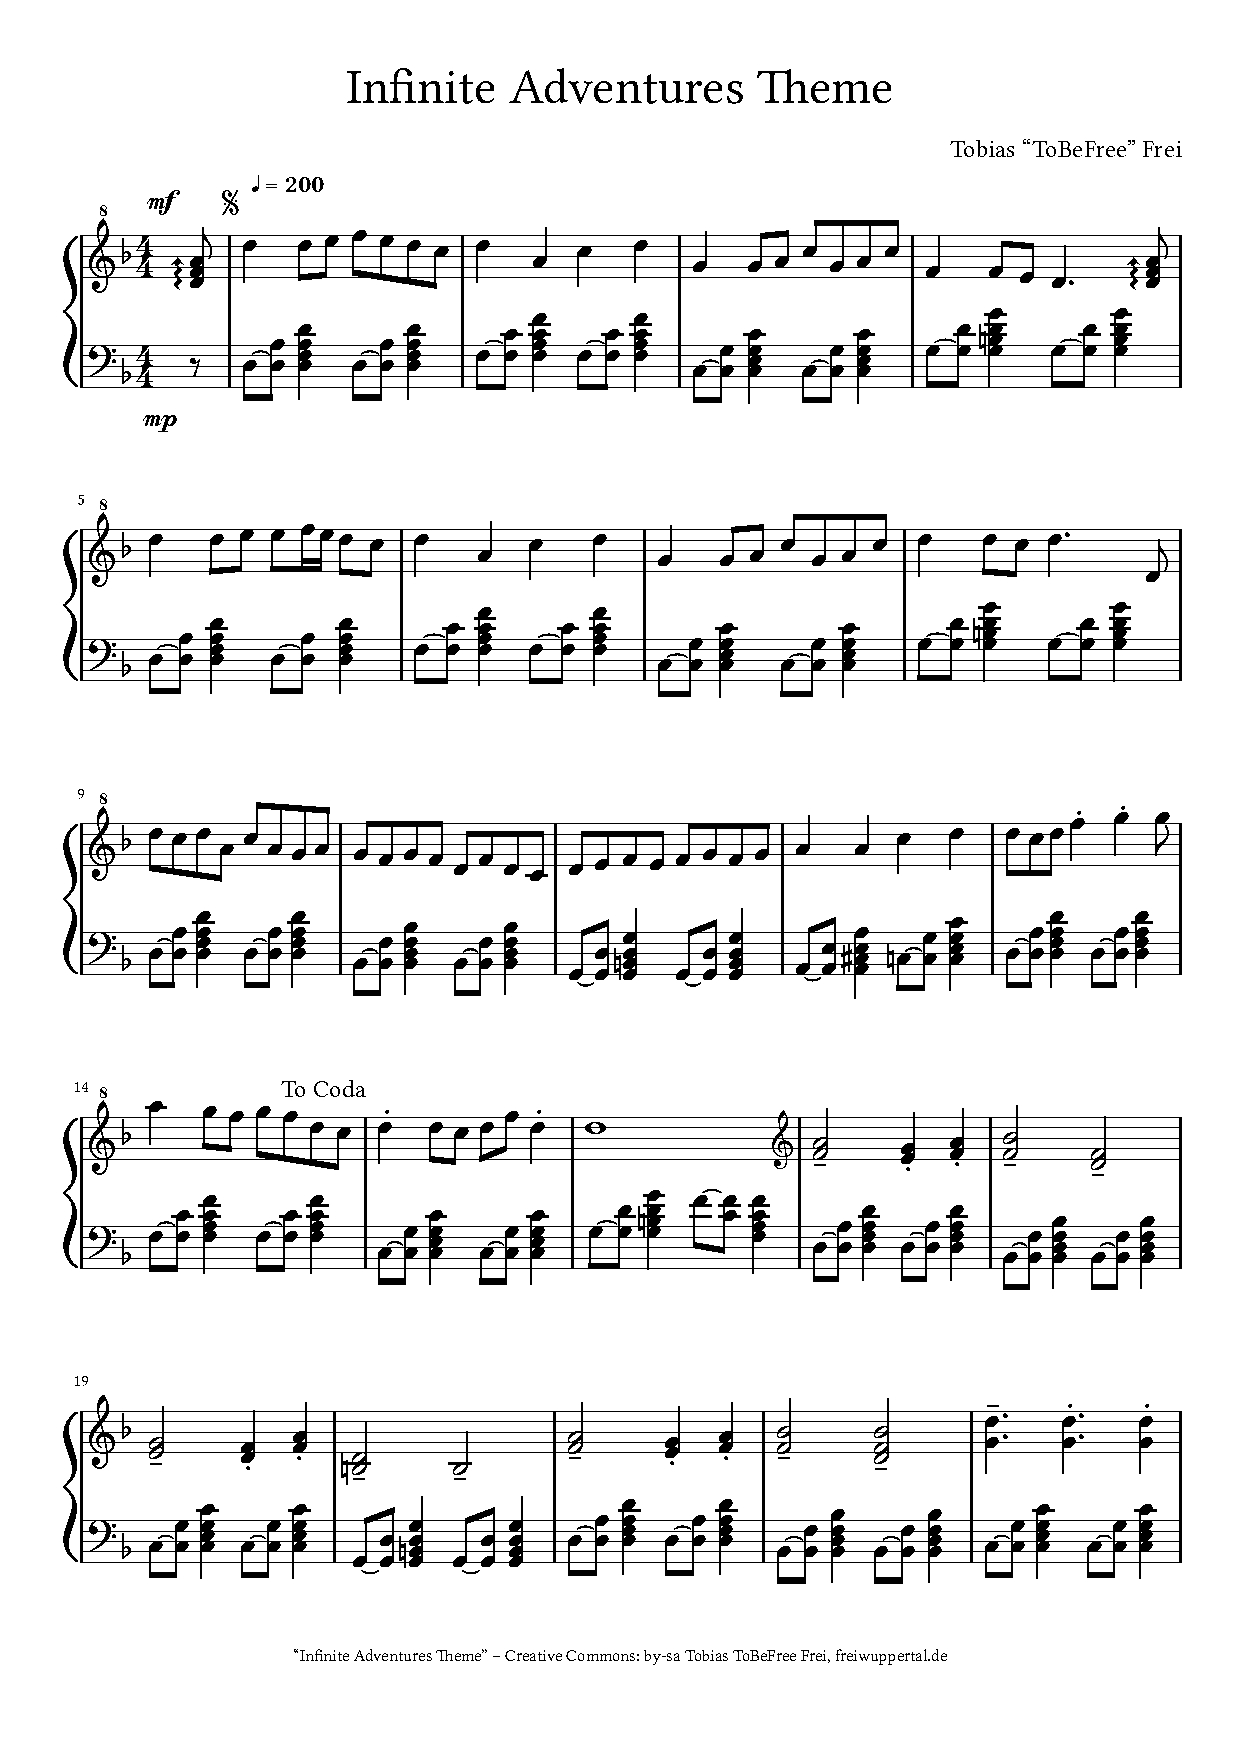
\includegraphics[width=\textwidth, page=1]{z-include-main-iatheme.pdf}
\end{figure}

\begin{figure}[p]
    \includegraphics[width=\textwidth, page=2]{z-include-main-iatheme.pdf}
\end{figure}


\chapter{Musikliste}

\textbf{Für Filmproduzenten, Träumer und Multitasking-Genies.}

\begin{itemize}
    \item Falls du ernsthaft einen Film zu diesem Buch drehen möchtest.
    \item Falls du das gesamte Buch bereits ausgelesen hast und die genannten Lieder vielleicht noch gar nicht kennst. Höre die Lieder und stelle dir dabei die Szenen vor. Wenn es schon keinen IA-Film gibt, kannst du wenigstens einen Film in deinem Kopf laufen lassen.
    \item Falls du beim Lesen Musik hören möchtest, die zur aktuellen Szene passt.
\end{itemize}

Diese Liste wurde von den Autoren zusammengestellt und impliziert keinerlei Unterstützung oder Befürwortung durch die Komponisten der Lieder.

Musik, die leider zum Veröffentlichungszeitpunkt nicht frei lizenziert war, ist durch \textit{kursiven Text} markiert. Eines Tages wird jedes dieser Lieder in die Gemeinfreiheit übergehen; der genaue Zeitpunkt hängt von verschiedenen Gesetzen ab.

Wir bieten auf infiniteadventures.de wahrscheinlich eine fertig nummerierte Musiksammlung der frei lizenzierten Lieder an, die einfach heruntergeladen und auf eine MP3-CD gebrannt werden kann. Für eine klassische Audio-CD ist die Gesamtlänge des Soundtracks deutlich zu groß.

Autoren der frei lizenzierten Musik:\\
Jason Shaw (Audionautix), audionautix.com\\
Marek »Wansti« Möckel, discarded-ideas.org\\
Nicolas Gasparini (Myuu), thedarkpiano.com\\
Tobias »ToBeFree« Frei, freiwuppertal.de

\begin{enumerate}
    \item Titelmelodie:\\ »Infinite Adventures Theme«~– Tobias »ToBeFree« Frei
    \item Orakel:\\ »Lazy Day«~– Jason Shaw (Audionautix)
    \item Fluchtauto mit Automatikgetriebe:\\ »All Good In The Wood«~– Jason Shaw (Audionautix)
    \item Kreuzfahrtschiff-Melodie (mehrfach verwendet):\\ »Bird In Hand«~– Jason Shaw (Audionautix)
    \item Verrückte Zugfahrt:\\ »Code Blue«~– Jason Shaw (Audionautix)
    \item Meister Orakel am Werk:\\ »Big Blues«~– Jason Shaw (Audionautix)
    \item Flug nach Mallorca:\\ »Jennys Theme«~– Jason Shaw (Audionautix)
    \item Die schwimmende Etage:\\ »Azitmuth«~– Jason Shaw (Audionautix)
    \item Kreuzfahrt nach Manhattan:\\ »Bird In Hand«~– Jason Shaw (Audionautix)
    \item Umrüstung des Helikopters:\\ »Boxcar Rag«~– Jason Shaw (Audionautix)
    \item Mit dem Helikopter um die Welt:\\ »Latin House Bed«~– Jason Shaw (Audionautix)
    \item Die Befreiung von Orakel in Südafrika:\\ »Boom«~– Jason Shaw (Audionautix)
    \item Verfolgungsjagd über China:\\ »Checks For Free«~– Jason Shaw (Audionautix)
    \item Mit dem Bus durch China:\\ »Busy Body«~– Jason Shaw (Audionautix)
    \item Alexandra:\\ \textit{»Satoris Theme, Third Eye« aus Touhou 11 (Chireiden, Subterranean Animism) von Jun'ya Ota (ZUN)}
    \item Überfall auf Fort Knox:\\ »Line of Fire«~– Jason Shaw (Audionautix)
    \item Flucht aus dem goldenen Gefängnis:\\ \textit{»The Ecstasy of Gold«~– Ennio Morricone}
    \item Einbruch beim FBI:\\ »Dark Mystery«~– Jason Shaw (Audionautix)
    \item Flug nach Kanada, Teil 1:\\ \textit{»Wings of Death, Level 5«~– Jochen Hippel (der Remix von Nils Schneider lohnt sich)}
    \item Flug nach Kanada, Teil 2:\\ »Med Tempo Rock«~– Jason Shaw (Audionautix)
    \item Greater Sudbury:\\ »Landras Dream«~– Jason Shaw (Audionautix)
    \item Am Lagerfeuer:\\ »Antarctica«~– Jason Shaw (Audionautix)
    \item Flucht vom Lagerfeuer:\\ \textit{»Run Away«~– Sunstroke Project, for Moldova at ESC 2010}
    \item Kanada nach USA, Teil 1:\\ \textit{»Wings of Death, Level 6«~– Jochen Hippel (auch zu diesem Lied hat Nils Schneider einen tollen Remix erstellt)}
    \item Kanada nach USA, Teil 2:\\ \textit{Im Text wird ein Lied erwähnt. Einfach im richtigen Moment abspielen.}
    \item Sprung in die Tiefe:\\ »Funky Junky«~– Jason Shaw (Audionautix)
    \item Bitte volltanken:\\ »Feel Good Rock«~– Jason Shaw (Audionautix)
    \item Boeing 737 nach Deutschland:\\ \textit{»Like a Tiger«~– Jayme Gutierrez (das Musikvideo ist gut)}
    \item Frees Theme:\\ \textit{»(Kenny the) Toffelskater«~– Kalle Jonsson (Dubmood)}
    \item Aus der Ferne dringende Musik vom Filmfestival:\\ »Boots! Boots! Boots!«~– Jason Shaw (Audionautix)
    \item Louvre-Mission:\\ »In Motion«~– Jason Shaw (Audionautix)
    \item Flucht aus dem Louvre:\\ \textit{»Satono Nishida \& Mai Teireida, Crazy Backup Dancers« aus Touhou 16 (Tenkuushou, Hidden Star in Four Seasons) von Jun'ya Ota (ZUN)}
    \item Flug ins All:\\ \textit{»Major Tom«~– Peter Schilling}
    \item Landung auf Örz:\\ Europahymne »Ode an die Freude«, ohne Text, letzter Satz der neunten Sinfonie in d-Moll op. 125~– Ludwig van Beethoven (gemeinfreie Version beispielsweise von der United States Navy Band)
    \item Dorf der Äöüzz:\\ »Forest Rhythm«~– Jason Shaw (Audionautix)
    \item Örzkäpitöl:\\ »In The Field«~– Jason Shaw (Audionautix)
    \item Betreten des Fööd-Geschäfts:\\ »Happy Little Elves«~– Jason Shaw (Audionautix)
    \item Eigenes Haus:\\ »Keep It Real«~– Jason Shaw (Audionautix)
    \item Reise der 4-6692 im Weltall:\\ \textit{»Journey of the Sorcerer«~– Eagles}
    \item Nuklearer Winter:\\ »The Angels Weep«~– Jason Shaw (Audionautix)
    \item Weltraum-Hintergrundmusik, wenn keine andere läuft:\\ »Deep Space«~– Jason Shaw (Audionautix)
    \item Anflug auf Cats Paw Sector OI-T c3-3:\\ »Go Not Gently«~– Jason Shaw (Audionautix)
    \item Friedliche Welt:\\ »Antarctica«~– Jason Shaw (Audionautix)
    \item Landung im Gebirge:\\ »Intense Suspense«~– Jason Shaw (Audionautix)
    \item Immer, wenn die Freunde sich draußen im Tal aufhalten:\\ »Calm Blue Lake«~– Jason Shaw (Audionautix)
    \item Im Inneren der Möribünd Explörer:\\ »Dark Mystery«~– Jason Shaw (Audionautix)
    \item Ohne Licht durch die Höhle:\\ Mit leiser Lautstärke im Hintergrund:\\ »High Tension«~– Jason Shaw (Audionautix)
    \item Alexandra im Einsatz:\\  \textit{»Sakuya Izayoi's Theme, Flowering Night« aus Touhou 10.5 (Hisouten, Scarlet Weather Rhapsody) von Jun'ya Ota (ZUN)}
    \item Gefecht über Blärg:\\ \textit{»Star Fox (SNES), Corneria«~– Hajime Hirasawa (der Remix von Qumu Music übertrifft das Original)}
    \item Sehenswürdigkeiten im Weltall:\\ »Leavin The Lights«~– Jason Shaw (Audionautix)
    \item derair:\\ »House of Evil«~– Jason Shaw (Audionautix)
    \item Raumgefecht:\\ »Fight Scene«~– Jason Shaw (Audionautix)
    \item Rückkehr nach Örz:\\ »Chasin’ It«~– Jason Shaw (Audionautix)
    \item Willkommen zurück:\\ »Shadow Of Truth«~– Jason Shaw (Audionautix)
    \item Verurteilt:\\ »Legends Of The River«~– Jason Shaw (Audionautix)
    \item Vierhändige Klaviermusik:\\ »Ungarischer Tanz Nr. 5, Klavierfassung in fis-Moll«~– Johannes Brahms
    \item Ankunft auf ugghy:\\ »Event Horizon«~– Jason Shaw (Audionautix)
    \item Ausbruch:\\ »Intro Action«~– Jason Shaw (Audionautix)
    \item Floating Island sucht Material:\\ »Energy Bed 2«~– Jason Shaw (Audionautix)
    \item Im Inneren des uggy-Raumschiffs auf Örs-Anflug:\\ »Harsh Alien Machine«~– Jason Shaw (Audionautix)
    \item Angriff der uggy-Zerstörungsflotte:\\ »Long Live Death«~– Jason Shaw (Audionautix)
    \item SoulOfTheInternet:\\ \textit{»Thraddash: Culture 19« (Remix des Liedes »Thraddash Theme« aus Star Control II, 1992, von Riku Nuottajärvi)~– Espen Gätzschmann und Tore Aune Fjellstad}
    \item SOTIs Welt:\\ »Ohm« von Audionautix
    \item Landung der Protagonisten auf der Erde:\\ »Lexicon«~– Jason Shaw (Audionautix)
    \item Das Haus, in dem noch alles normal ist:\\ »Paper Wings« von Audionautix
    \item Überraschung im BIDWA:\\ »Peppers Funk«~– Jason Shaw (Audionautix)
    \item Vorbereitung:\\ »Doghouse«~– Jason Shaw (Audionautix)
    \item Credits am Ende:\\ \textit{»Cydonian Sky«~– Dubmood (Kalle Jonsson)}
    \item \textbf{Generelle Vorschläge für Zeit-Vergeht-Szenen:}\\ »Forest Theme for Piano and Recorder«~– Marek »Wansti« Möckel
    \item »Forest Dance«~– Marek »Wansti« Möckel
    \item »Rabbit Holes«~– Marek »Wansti« Möckel
    \item »Riding The Wind«~– Marek »Wansti« Möckel
    \item »Nightfall«~– Marek »Wansti« Möckel
    \item »Phase Shifter«~– Jason Shaw (Audionautix)
    \item »Opus One«~– Jason Shaw (Audionautix)
    \item »Pop Rock Bed«~– Jason Shaw (Audionautix)
    \item »Over Time«~– Jason Shaw (Audionautix)
    \item »Time Passing By«~– Jason Shaw (Audionautix)
    \item »The Voyage«~– Jason Shaw (Audionautix)
    \item »Triangle«~– Jason Shaw (Audionautix)
    \item »In A World«~– Jason Shaw (Audionautix)
    \item »Quiet«~– Jason Shaw (Audionautix)
    \item »Renaissance«~– Jason Shaw (Audionautix)
    \item »River Meditation«~– Jason Shaw (Audionautix)
    \item »Serious Drama«~– Jason Shaw (Audionautix)
    \item »Serious Piano«~– Jason Shaw (Audionautix)
    \item »Evil Returns«~– Nicolas Gasparini (Myuu)
    \item »Moonlight Menschen«~– Nicolas Gasparini (Myuu)
    \item \textit{»Extra Stage Theme, Last Remote« aus Touhou 11 (Chireiden, Subterranean Animism) von Jun'ya Ota (ZUN)}
    \item \textit{»Hong Meiling's Theme, Shanghai Alice of Meiji 17« aus Touhou 6 (Koumakyou, the Embodiment of Scarlet Devil) von Jun'ya Ota (ZUN)}
    \item \textit{»Reimu Hakurei's Theme, Dichromatic Lotus Butterfly / Ancients« aus Touhou 12.3 (Hisoutensoku, Unthinkable Natural Law) von Jun'ya Ota (ZUN)}
    \item \textit{»Reimu Hakurei's Theme, Dichromatic Lotus Butterfly / Red and White« aus Touhou 14.5 (Shinpiroku, Urban Legend in Limbo) von Jun'ya Ota (ZUN) und Comp von Butaotome}
    \item \textit{»Sweet Dreams«~– Jussi-Matti Salmela (Elwood)}
    \item \textbf{Generelle Vorschläge für Action-Szenen:}\\ »Prophecy«~– Marek »Wansti« Möckel
    \item »Fortress«~– Marek »Wansti« Möckel
    \item »Ectoplasm«~– Jason Shaw (Audionautix)
    \item »Delusion 32«~– Jason Shaw (Audionautix)
    \item »Pop Metal«~– Jason Shaw (Audionautix)
    \item »Bustin Loose« / »Bustin Loose W Lead«~– Jason Shaw (Audionautix)
    \item »Pentagram«~– Jason Shaw (Audionautix)
    \item »Periscope«~– Jason Shaw (Audionautix)
    \item »Sports Action«~– Jason Shaw (Audionautix)
    \item »Pyramids«~– Jason Shaw (Audionautix)
    \item »Night Runner«~– Jason Shaw (Audionautix)
    \item \textit{»Cirno's Theme, Otenba Koi Musume / Tomboyish Girl in Love« aus Touhou 12.3 (Hisoutensoku, Unthinkable Natural Law) von Jun'ya Ota (ZUN)}
    \item \textit{»Eirin Yagokoro's Theme, Gensokyo Millenium / History of the Moon« aus Touhou 08 (Eiyashou, Imperishable Night) von Jun'ya Ota (ZUN)}
    \item \textit{»Fujiwara no Mokou's Theme, Reach for the Moon, Immortal Smoke« aus Touhou 08 (Eiyashou, Imperishable Night) von Jun'ya Ota (ZUN)}
    \item \textit{»Irresistible«~– Fall Out Boy}
    \item \textit{»Immortals« ~– Fall Out Boy}
    \item \textit{»Megalovania« (aus Undertale von Toby Fox)}

\end{enumerate}


\chapter{Kleines Lexikon}

\begin{itemize}
    \item \textbf{ISG:}\\ IntärStällär Gräm, InterStellare Gewichtseinheit. 1 ISG ist die Masse von $3*7^{29}$ Silicium-28-Atomen. Daher gilt: $1 ISG ≈ 0.4487593$ Kilogramm.
    \item \textbf{Örztempz:}\\ Absolute Temperaturskala der Äöüzz. 1 Örztemp ist die thermodynamische Temperatur des Tripelpunktes des Wassers geteilt durch 7³. Daher gilt: 1 Örztemp = (343/273.16) Kelvin.
    \item \textbf{Septillion:}\\ nicht nur wegen der Sieben, sondern auch wegen $10^{42}$
    \item \textbf{117649:}\\ $1000000₇$
    \item \textbf{1460:}\\ Anzahl der Ziffern von $2^{4096}$ nach einer Umrechnung ins Siebenersystem.
    \item \textbf{1602…17…66208:}\\ Elementarladung: $e ≈ 1.6021766208*10^{-19}$ Coulomb
    \item \textbf{1984:}\\ Titel eines Romans von Eric Arthur Blair (»George Orwell«)
    \item \textbf{210:}\\ $420₇$ (schöner Zufall: Multiplikation mit 2 ergibt base7-Zahl.)
    \item \textbf{2401:}\\ $10000₇$
    \item \textbf{27729:}\\ $15.5151…₇$
    \item \textbf{29:}\\ Siebenersystem-Äquivalent zu 'Turn it up to Eleven': Turn it up to 41₇
    \item \textbf{30:}\\ $42₇$
    \item \textbf{3294172:}\\ $40000000₇$
    \item \textbf{3306:}\\ Standard-Port einer beliebten SQL-Software
    \item \textbf{34.98:}\\ $46.66₇$
    \item \textbf{36015:}\\ $50000₇ * 3$
    \item \textbf{400:}\\ Zufall: $1111₇$
    \item \textbf{41996493₁₀:}\\ $3294172₁₀*12.75₁₀*0.9999₁₀$
    \item \textbf{42:}\\ Douglas Adams: Antwort auf die Frage nach dem Leben, dem Universum und dem ganzen Rest
    \item \textbf{42000693₁₀ (ca. 42 Millionen):}\\ $3294172₁₀*12.75₁₀$
    \item \textbf{43597…44650:}\\ Hartree-Energie: $Eh ≈ 4.359744650*10^{-18}$ Joule
    \item \textbf{4.6692:}\\ Feigenbaum-Konstante (Chaoskonstante) $δ ≈ 4.6692016091$
    \item \textbf{496:}\\ dritte perfekte Zahl: $1+2+4+8+16+31+62+124+248 = 496$
    \item \textbf{618033989:}\\ Goldener Schnitt: $Φ = \frac{1+\sqrt{5}}{2} ≈ 1.6180339887$
    \item \textbf{630:}\\ Durch 3 teilbar und auch im Siebenersystem eine runde Zahl: 1560₇
    \item \textbf{70:}\\ Auch im Siebenersystem eine runde Zahl: 130₇
    \item \textbf{7320508:}\\ Erste Nachkommastellen von $\sqrt{3}$
    \item \textbf{9109383:}\\ Elektronenmasse: $me ≈ 9.109383*10^{-31}$ Kilogramm
\end{itemize}


\chapter{Orakels Zeichnungen}

Als das Freiwuppertal-Forum noch aktiv genutzt wurde, hat Orakel einige Zeichnungen erstellt, in denen die Forenbenutzer satirisch dargestellt wurden. Da die Protagonisten der Infinite Adventures ihre Namen von den Benutzern dieses Forums erhalten haben, sind gewisse Überschneidungen mit dem Inhalt des Romans erkennbar. Die Zeichnungen wurden \textit{nicht} für die Infinite Adventures erstellt, dürfen aber als ergänzendes Bonusmaterial nicht fehlen.

Wir werden voraussichtlich einen DIN-A4-Bonusband zu den Infinite Adventures veröffentlichen. Eine Ringbindung soll leichtes Umblättern und Herausnehmen des Bonusmaterials ermöglichen. In diesem Bonusband werden möglicherweise weitere Zeichnungen enthalten sein.

\begin{figure}[p]
    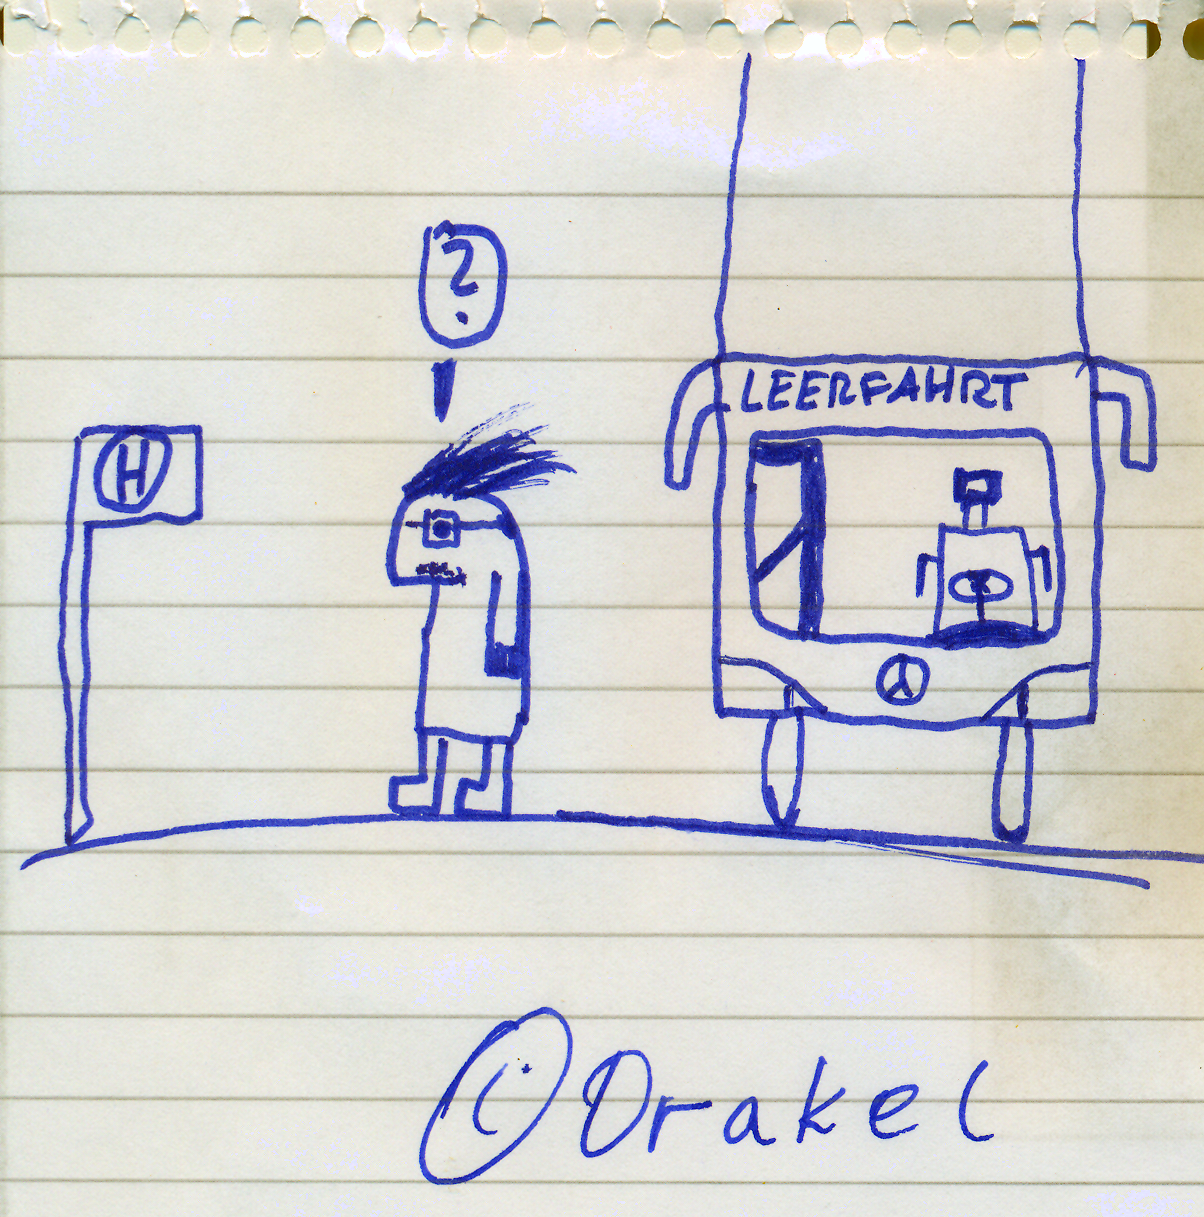
\includegraphics[width=\linewidth]{z-include-main-oleerfahrt.png}
    \caption{„Leerfahrt“. CC by-sa 4.0: Mirco Hensel}
\end{figure}

\begin{figure}[p]
    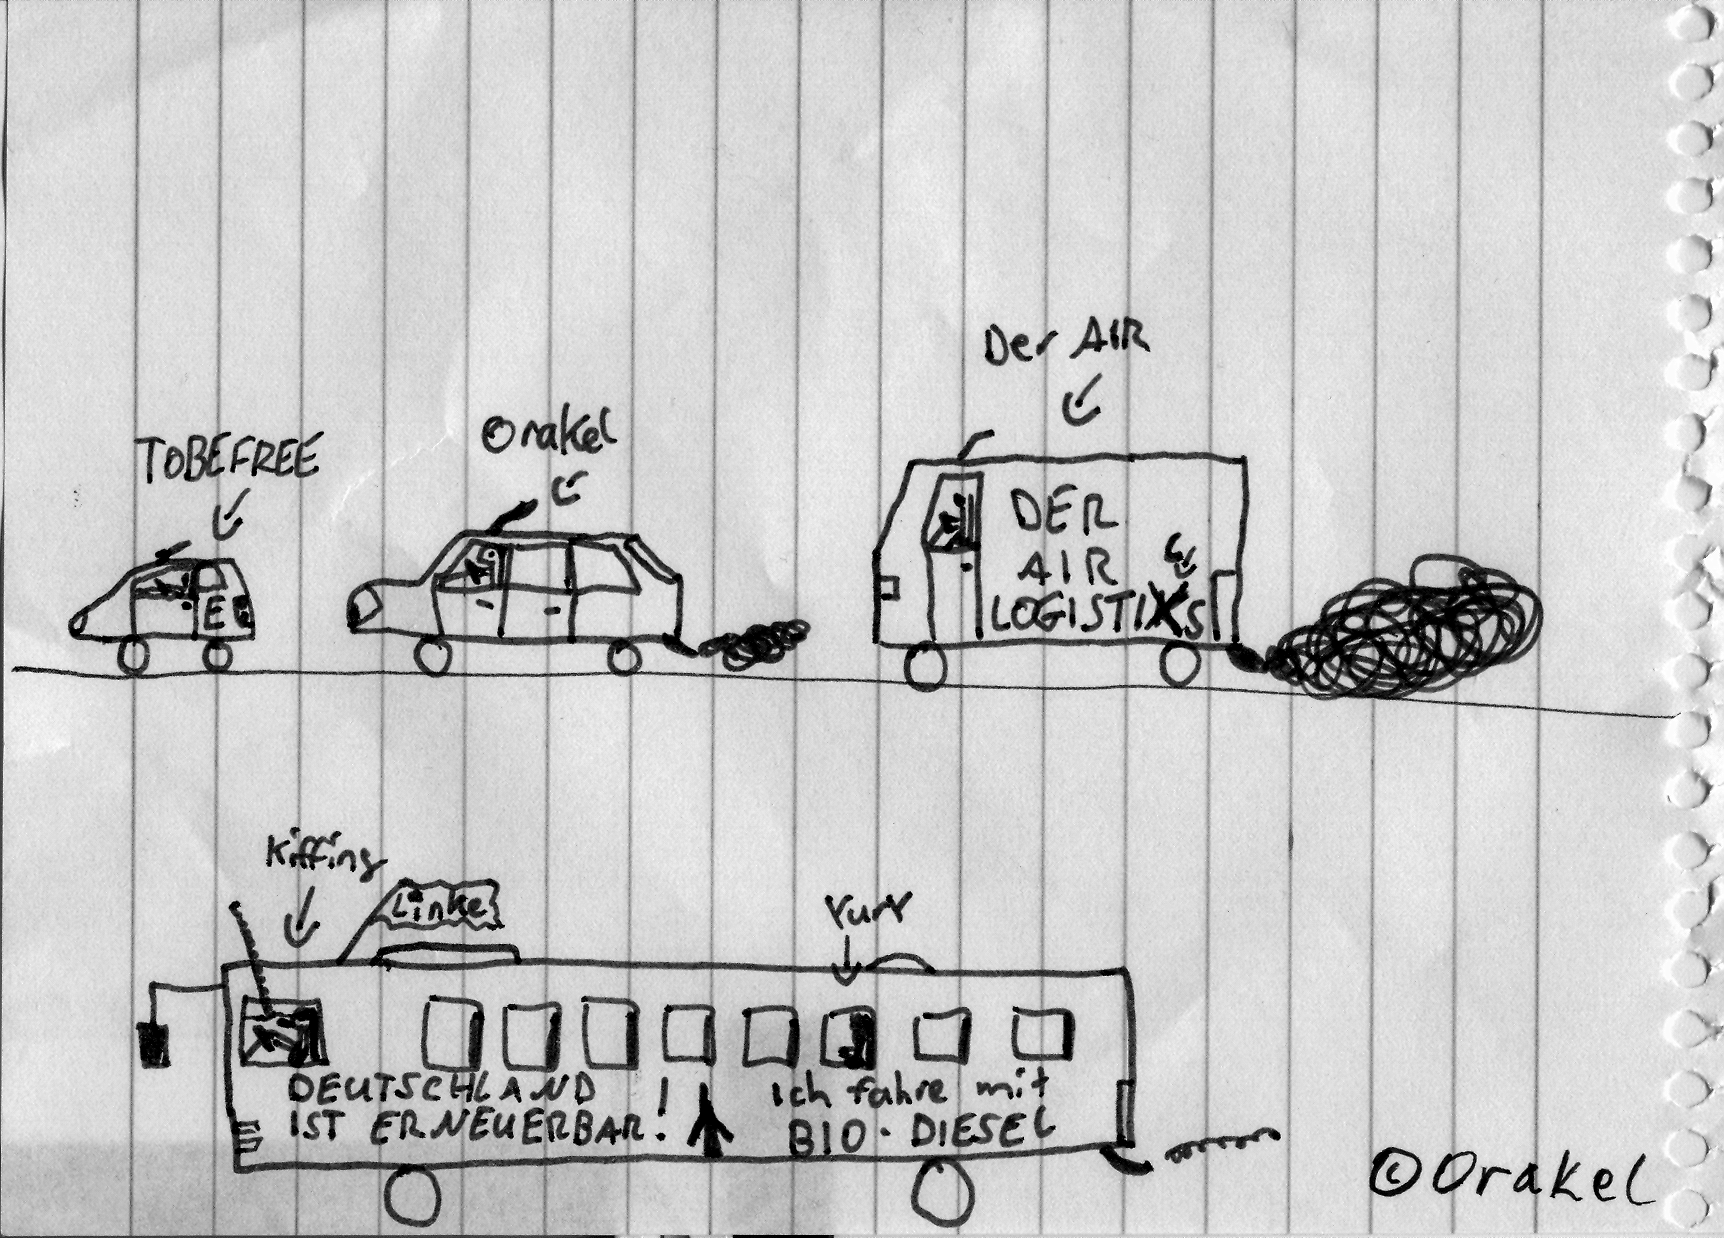
\includegraphics[width=\linewidth]{z-include-main-omotion.png}
    \caption{„Motion“. CC by-sa 4.0: Mirco Hensel}
\end{figure}


\chapter{Karte der Galaxis}

Auch diese Karte wird möglicherweise in größerem Format zu einem Teil des Bonusbands werden.

\begin{figure}[p]
    
\includegraphics[width=\linewidth]{z-include-main-squaremap1.jpg}
    \caption{Unsere Milchstraße}
\end{figure}

\begin{figure}[p]
    
\includegraphics[width=\linewidth]{z-include-main-squaremap2.jpg}
    \caption{Galaktisches Koordinatensystem}
\end{figure}


\chapter{Auszug: Original-Forenthread}

So sind die Infinite Adventures entstanden: Orakel, yury und Free haben Beiträge in einem Internetforum geschrieben. In diesem Auszug sieht man, wie innerhalb von vier Stunden alle drei Autoren einen Teil zum Roman beigetragen haben. Außerdem ist dies der Beweis dafür, dass wir bereits im September 2010 das Aufkommen von Quantencomputern und DNA-Festplatten vorhergesagt haben.

Orakels Beitrag enthält ein Handygespräch, das damals noch über mehrere Galaxien hinweg geführt wurde. Auch in der heutigen Fassung mit einer Distanz von über 4000 Lichtjahren zur Erde verfehlt der Anruf seine überraschende Wirkung nicht.

Auf die Idee, man könnte die aus Fort Knox gestohlenen Goldbarren auf Örz verkaufen, waren wir damals noch nicht gekommen. Daher muss Free für den Quantencomputer einen Kredit aufnehmen. Dass schwere körperliche Arbeit auf dem fortschrittlichen Planeten nicht von Robotern erledigt wurde, wirkt im Nachhinein merkwürdig.

yury überraschte uns dann mit einer Verhaftung aus heiterem Himmel. Sein Kommentar dazu: »Ich hab schon einen Hintergedanken, aber der Plan ist doch, dass ihr jetzt was völlig anderes, für mich unerwartetes schreibt und die IA dadurch interessant wird… also lasst euch was einfallen! ;)«

Das Design des Forums hat sich irgendwann durch ein Update geändert; dieses aktuelle Bildschirmfoto zeigt nicht das ursprüngliche Aussehen des Forums. Zudem fällt auf, dass die Geschichte damals einen anderen Titel hatte und dass Free anders hieß.

\begin{figure}[p]
    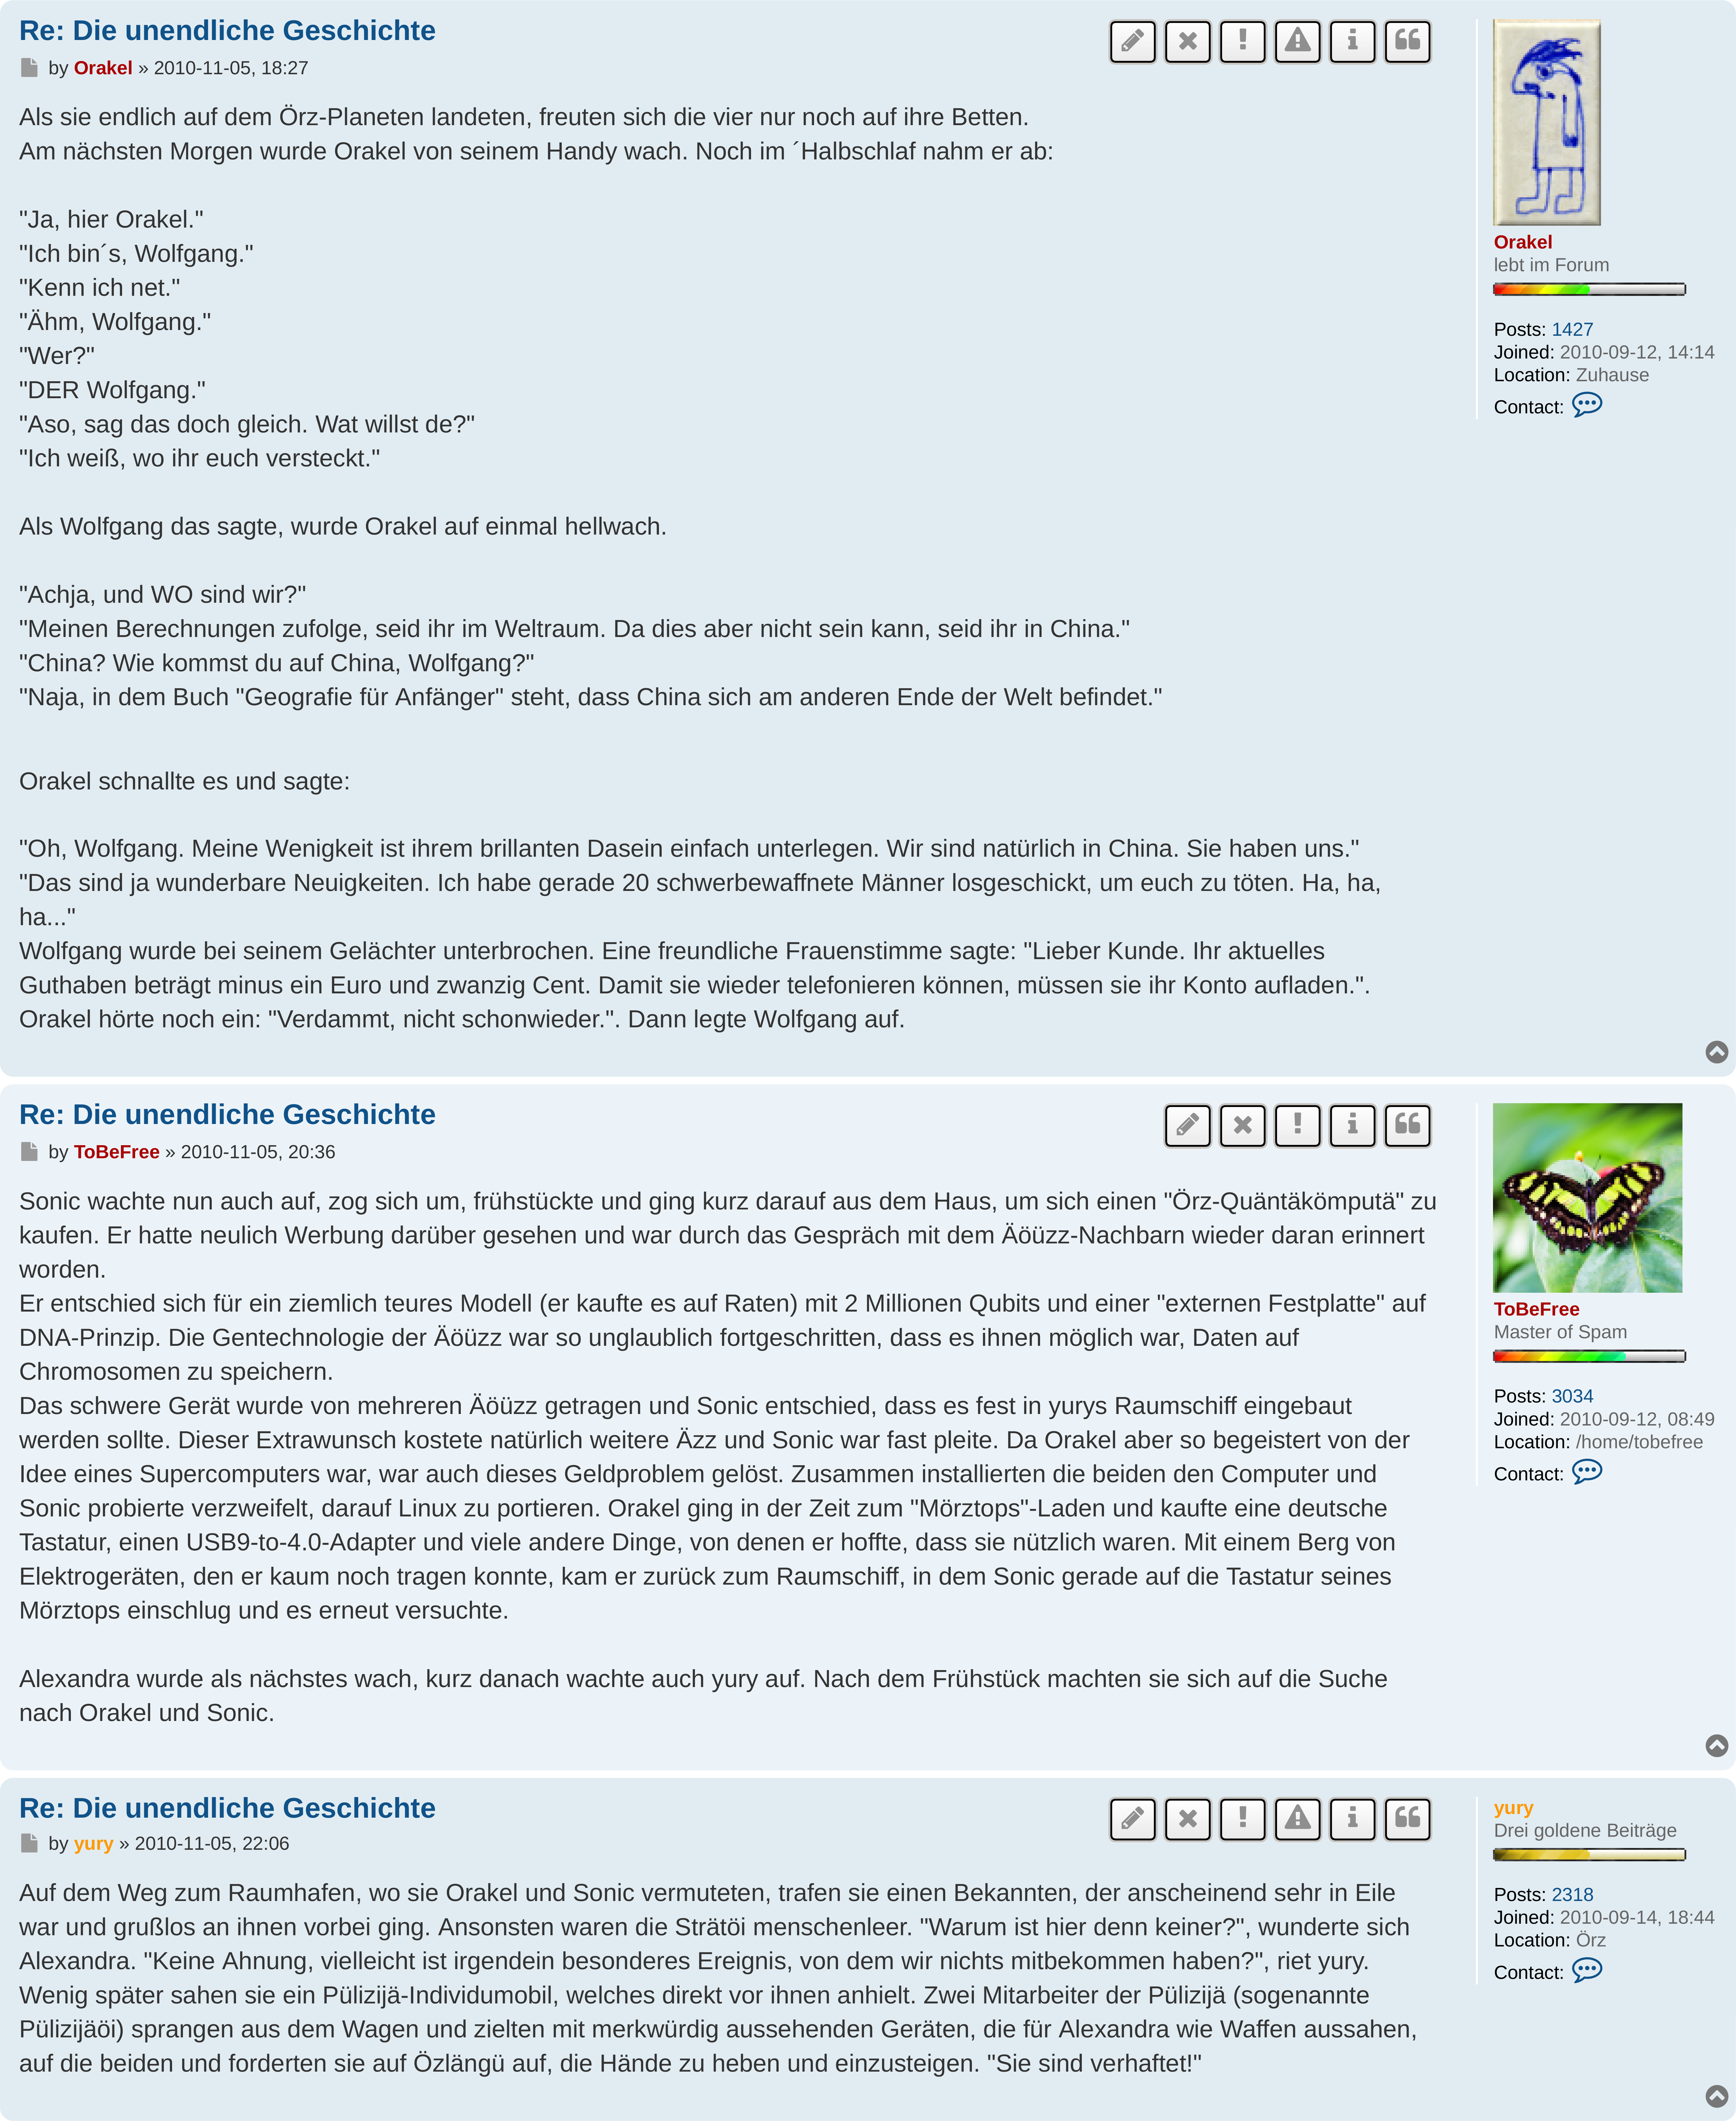
\includegraphics[width=\linewidth]{z-include-main-forum.png}
    \caption{https://freiwuppertal.de/forum\#: Interner Schreibbereich}
\end{figure}


\chapter{Bildquellen}

Alle verwendeten Bilder sind frei lizenziert. Die Verwendung der Bilder in diesem Roman impliziert keinerlei Unterstützung oder Befürwortung durch ihre Schöpfer.

\begin{itemize}
    \item \textbf{Buchcover:} CC0-Lizenz / Public Domain.\\ Yuri\_B, pixabay.com
    \item \textbf{Teil-2-Titelbild:} CC0-Lizenz / Public Domain.\\ Leandro Barco (Wortley, pixabay.com)
    \item \textbf{Galaktische Karte:} Public Domain.\\ NASA/JPL-Caltech/R. Hurt (SSC/Caltech).\\ https://commons.wikimedia.org/wiki/\\File:236084main\_MilkyWay-full-annotated.jpg
    \item \textbf{NGC 6188/6193 und NGC 6334:} Public Domain.\\ Dylan O'Donnell, deography.com\\ »That means it’s free for you to use, now and forever. You don’t even have to credit me for it. […] Photography is not my job and I’d rather not kill any enthusiasm I have for it by accepting money for the obligation to take photos.

So use them, by all means. You don’t have to credit me if you don’t want to, but I love seeing my work out there in the wild being used, mixed and remixed. Send me a link, I’d love to see what you do!« (https://deography.com/yes-its-free/\#, Abruf 2018-01-01)
    \item \textbf{Lagrange-Punkte:} Public Domain.\\ Originalbild: NASA / WMAP Science Team.\\ WMAP-Sonde entfernt, Kontrast verbessert, Kompressionsartefakte verringert.\\ https://commons.wikimedia.org/wiki/\\File:Lagrange.jpg\\ https://commons.wikimedia.org/wiki/\\File:Lagrange-better.png
    \item \textbf{Helixnebel (NGC 7293):} Public Domain.\\ NASA/JPL-Caltech.\\ https://commons.wikimedia.org/wiki/\\File:Helix\_Nebula\_-\_Unraveling\_at\_the\_Seams.jpg
    \item \textbf{Orakels Zeichnungen und Orakels Avatar:}\\ Creative Commons by-sa 4.0.\\ Mirco Hensel\\Eine Kopie der Lizenz befindet sich am Ende des Buches.
    \item \textbf{ToBeFrees Avatar:}\\ CC0-Lizenz / Public Domain.\\ jill111, pixabay.com
\end{itemize}

Bei den Bildern in diesem Roman handelt es sich nicht um die exakten Originalbilder, sondern um Abwandlungen (Weißabgleich, Helligkeit, Kontrast, Sättigung, Schärfung, Zuschnitt etc.) erstellt durch Tobias Frei.

Für die Infinite Adventures erstellte Abwandlungen frei lizenzierter Werke wurden auf Wikimedia Commons hochgeladen und auf diese Weise an die Gemeinschaft zurückgegeben.

Yuri\_B, Leandro Barco und Dylan O'Donnell erhalten jeweils mindestens ein kostenloses Exemplar des Buches. Zum Dank für die frei nutzbaren Bilder wird persönliches Bonusmaterial erstellt.


\chapter{Lizenz des Buchinhalts}

\textbf{Infinite Adventures © by\\ Mirco Hensel, yury und Tobias Frei, infiniteadventures.de}

Dies ist eine offizielle Ausgabe der Infinite Adventures, herausgegeben von Tobias Frei. Veränderte Versionen und unautorisierte Nachdrucke müssen deutlich als solche erkennbar sein. Auch das Impressum muss angepasst werden, wenn das Dokument verändert wird.

Falls Du die Rechte in dieser Lizenz nutzen möchtest, musst Du sie vollständig gelesen und verstanden haben. Es genügt nicht, nur eine Zusammenfassung zu lesen. Aus diesem Grund bieten wir keine solche Zusammenfassung an.

This novel is licensed under a Creative Commons Attribution-ShareAlike 4.0 International License.

You should have received a copy of the license along with this work. If not, see\\
https://creativecommons.org/licenses/by-sa/4.0/legalcode

You are required to actually read and understand the full text of the license, not a summary.

\begin{center}
    \large{\textbf{Creative Commons Attribution-ShareAlike 4.0 International Public License}}
\end{center}

By exercising the Licensed Rights (defined below), You accept and agree to be bound by the terms and conditions of this Creative Commons Attribution-ShareAlike 4.0 International Public License ("Public License"). To the extent this Public License may be interpreted as a contract, You are granted the Licensed Rights in consideration of Your acceptance of these terms and conditions, and the Licensor grants You such rights in consideration of benefits the Licensor receives from making the Licensed Material available under these terms and conditions.

\begin{center}
    \textbf{Section 1 -- Definitions.}
\end{center}

\begin{itemize}
    \item[a.] \textbf{Adapted Material} means material subject to Copyright and Similar Rights that is derived from or based upon the Licensed Material and in which the Licensed Material is translated, altered, arranged, transformed, or otherwise modified in a manner requiring permission under the Copyright and Similar Rights held by the Licensor. For purposes of this Public License, where the Licensed Material is a musical work, performance, or sound recording, Adapted Material is always produced where the Licensed Material is synched in timed relation with a moving image.
    \item[b.] \textbf{Adapter's License} means the license You apply to Your Copyright and Similar Rights in Your contributions to Adapted Material in accordance with the terms and conditions of this Public License.
    \item[c.] \textbf{BY-SA Compatible License} means a license listed at creativecommons.org/compatiblelicenses, approved by Creative Commons as essentially the equivalent of this Public License.
    \item[d.] \textbf{Copyright and Similar Rights} means copyright and/or similar rights closely related to copyright including, without limitation, performance, broadcast, sound recording, and Sui Generis Database Rights, without regard to how the rights are labeled or categorized. For purposes of this Public License, the rights specified in Section 2(b)(1)-(2) are not Copyright and Similar Rights.
    \item[e.] \textbf{Effective Technological Measures} means those measures that, in the absence of proper authority, may not be circumvented under laws fulfilling obligations under Article 11 of the WIPO Copyright Treaty adopted on December 20, 1996, and/or similar international agreements.
    \item[f.] \textbf{Exceptions and Limitations} means fair use, fair dealing, and/or any other exception or limitation to Copyright and Similar Rights that applies to Your use of the Licensed Material.
    \item[g.] \textbf{License Elements} means the license attributes listed in the name of a Creative Commons Public License. The License Elements of this Public License are Attribution and ShareAlike.
    \item[h.] \textbf{Licensed Material} means the artistic or literary work, database, or other material to which the Licensor applied this Public License.
    \item[i.] \textbf{Licensed Rights} means the rights granted to You subject to the terms and conditions of this Public License, which are limited to all Copyright and Similar Rights that apply to Your use of the Licensed Material and that the Licensor has authority to license.
    \item[j.] \textbf{Licensor} means the individual(s) or entity(ies) granting rights under this Public License.
    \item[k.] \textbf{Share} means to provide material to the public by any means or process that requires permission under the Licensed Rights, such as reproduction, public display, public performance, distribution, dissemination, communication, or importation, and to make material available to the public including in ways that members of the public may access the material from a place and at a time individually chosen by them.
    \item[l.] \textbf{Sui Generis Database Rights} means rights other than copyright resulting from Directive 96/9/EC of the European Parliament and of the Council of 11 March 1996 on the legal protection of databases, as amended and/or succeeded, as well as other essentially equivalent rights anywhere in the world.
    \item[m.] \textbf{You} means the individual or entity exercising the Licensed Rights under this Public License. Your has a corresponding meaning.
\end{itemize}

\begin{center}
    \textbf{Section 2 -- Scope.}
\end{center}

\begin{itemize}
    \item[a.] \textbf{License grant.}
    \begin{itemize}
        \item[1.] Subject to the terms and conditions of this Public License, the Licensor hereby grants You a worldwide, royalty-free, non-sublicensable, non-exclusive, irrevocable license to exercise the Licensed Rights in the Licensed Material to:
        \begin{itemize}
            \item[A.] reproduce and Share the Licensed Material, in whole or in part; and
            \item[B.] produce, reproduce, and Share Adapted Material.
        \end{itemize}
        \item[2.] \underline{Exceptions and Limitations}. For the avoidance of doubt, where Exceptions and Limitations apply to Your use, this Public License does not apply, and You do not need to comply with its terms and conditions.
        \item[3.] \underline{Term}. The term of this Public License is specified in Section 6(a).
        \item[4.] \underline{Media and formats; technical modifications allowed}. The Licensor authorizes You to exercise the Licensed Rights in all media and formats whether now known or hereafter created, and to make technical modifications necessary to do so. The Licensor waives and/or agrees not to assert any right or authority to forbid You from making technical modifications necessary to exercise the Licensed Rights, including technical modifications necessary to circumvent Effective Technological Measures. For purposes of this Public License, simply making modifications authorized by this Section 2(a)(4) never produces Adapted Material.
        \item[5.] \underline{Downstream recipients}.
        \begin{itshape}\begin{itemize}
            \item[A.] \underline{Offer from the Licensor -- Licensed Material}. Every recipient of the Licensed Material automatically receives an offer from the Licensor to exercise the Licensed Rights under the terms and conditions of this Public License.
            \item[B.] \underline{Additional offer from the Licensor -- Adapted Material}. Every recipient of Adapted Material from You automatically receives an offer from the Licensor to exercise the Licensed Rights in the Adapted Material under the conditions of the Adapter's License You apply.
            \item[C.] \underline{No downstream restrictions}. You may not offer or impose any additional or different terms or conditions on, or apply any Effective Technological Measures to, the Licensed Material if doing so restricts exercise of the Licensed Rights by any recipient of the Licensed Material.
        \end{itemize}\end{itshape}
        \item[6.] \underline{No endorsement}. Nothing in this Public License constitutes or may be construed as permission to assert or imply that You are, or that Your use of the Licensed Material is, connected with, or sponsored, endorsed, or granted official status by, the Licensor or others designated to receive attribution as provided in Section 3(a)(1)(A)(i).
    \end{itemize}
    \item[b.] \textbf{Other rights.}
    \begin{itemize}
        \item[1.] Moral rights, such as the right of integrity, are not licensed under this Public License, nor are publicity,
          privacy, and/or other similar personality rights; however, to the extent possible, the Licensor waives and/or agrees not to assert any such rights held by the Licensor to the limited extent necessary to allow You to exercise the Licensed Rights, but not otherwise.
        \item[2.] Patent and trademark rights are not licensed under this Public License.
        \item[3.] To the extent possible, the Licensor waives any right to collect royalties from You for the exercise of the Licensed Rights, whether directly or through a collecting society under any voluntary or waivable statutory or compulsory licensing scheme. In all other cases the Licensor expressly reserves any right to collect such royalties.
    \end{itemize}

\end{itemize}

\begin{center}
    \textbf{Section 3 -- License Conditions.}
\end{center}

Your exercise of the Licensed Rights is expressly made subject to the following conditions.

\begin{itemize}
    \item[a.] \textbf{Attribution.}
    \begin{itemize}
        \item[1.] If You Share the Licensed Material (including in modified form), You must:
        \begin{itemize}
            \item[A.] retain the following if it is supplied by the Licensor with the Licensed Material:
            \begin{itemize}
                \item[i.] identification of the creator(s) of the Licensed Material and any others designated to receive attribution, in any reasonable manner requested by the Licensor (including by pseudonym if designated);
                \item[ii.] a copyright notice;
                \item[iii.] a notice that refers to this Public License;
                \item[iv.] a notice that refers to the disclaimer of warranties;
                \item[v.] a URI or hyperlink to the Licensed Material to the extent reasonably practicable;
            \end{itemize}
            \item[B.] indicate if You modified the Licensed Material and retain an indication of any previous modifications; and
            \item[C.] indicate the Licensed Material is licensed under this Public License, and include the text of, or the URI or hyperlink to, this Public License.
        \end{itemize}
        \item[2.] You may satisfy the conditions in Section 3(a)(1) in any reasonable manner based on the medium, means, and context in which You Share the Licensed Material. For example, it may be reasonable to satisfy the conditions by providing a URI or hyperlink to a resource that includes the required information.
        \item[3.] If requested by the Licensor, You must remove any of the information required by Section 3(a)(1)(A) to the extent reasonably practicable.
    \end{itemize}
    \item[b.] \textbf{ShareAlike.}

     In addition to the conditions in Section 3(a), if You Share Adapted Material You produce, the following conditions also apply.

    \begin{itemize}
        \item[1.] The Adapter's License You apply must be a Creative Commons license with the same License Elements, this version or later, or a BY-SA Compatible License.
        \item[2.] You must include the text of, or the URI or hyperlink to, the Adapter's License You apply. You may satisfy this condition in any reasonable manner based on the medium, means, and context in which You Share Adapted Material.
        \item[3.] You may not offer or impose any additional or different terms or conditions on, or apply any Effective Technological Measures to, Adapted Material that restrict exercise of the rights granted under the Adapter's License You apply.
    \end{itemize}
\end{itemize}

\begin{center}
    \textbf{Section 4 -- Sui Generis Database Rights.}
\end{center}

Where the Licensed Rights include Sui Generis Database Rights that apply to Your use of the Licensed Material:

\begin{itemize}
    \item[a.] for the avoidance of doubt, Section 2(a)(1) grants You the right to extract, reuse, reproduce, and Share all or a substantial portion of the contents of the database;
    \item[b.] if You include all or a substantial portion of the database contents in a database in which You have Sui Generis Database Rights, then the database in which You have Sui Generis Database Rights (but not its individual contents) is Adapted Material, including for purposes of Section 3(b); and
    \item[c.] You must comply with the conditions in Section 3(a) if You Share all or a substantial portion of the contents of the database.
\end{itemize}

For the avoidance of doubt, this Section 4 supplements and does not replace Your obligations under this Public License where the Licensed Rights include other Copyright and Similar Rights.

\begin{center}
    \textbf{Section 5 -- Disclaimer of Warranties and Limitation of Liability.}
\end{center}

\begin{itemize}
    \item[\textbf{a.}] \textbf{Unless otherwise separately undertaken by the Licensor, to the extent possible, the Licensor offers the Licensed Material as-is and as-available, and makes no representations or warranties of any kind concerning the Licensed Material, whether express, implied, statutory, or other. This includes, without limitation, warranties of title, merchantability, fitness for a particular purpose, non-infringement, absence of latent or other defects, accuracy, or the presence or absence of errors, whether or not known or discoverable. Where disclaimers of warranties are not allowed in full or in part, this disclaimer may not apply to You.}
    \item[\textbf{b.}] \textbf{To the extent possible, in no event will the Licensor be liable to You on any legal theory (including, without limitation, negligence) or otherwise for any direct, special, indirect, incidental, consequential, punitive, exemplary, or other losses, costs, expenses, or damages arising out of this Public License or use of the Licensed Material, even if the Licensor has been advised of the possibility of such losses, costs, expenses, or damages. Where a limitation of liability is not allowed in full or in part, this limitation may not apply to You.}
    \item[c.] The disclaimer of warranties and limitation of liability provided above shall be interpreted in a manner that, to the extent possible, most closely approximates an absolute disclaimer and waiver of all liability.
\end{itemize}

\begin{center}
    \textbf{Section 6 -- Term and Termination.}
\end{center}

\begin{itemize}
    \item[a.] This Public License applies for the term of the Copyright and Similar Rights licensed here. However, if You fail to comply with this Public License, then Your rights under this Public License terminate automatically.

    \item[b.] Where Your right to use the Licensed Material has terminated under Section 6(a), it reinstates:

    \begin{itemize}
        \item[1.] automatically as of the date the violation is cured, provided it is cured within 30 days of Your discovery of the violation; or

        \item[2.] upon express reinstatement by the Licensor.
    \end{itemize}

     For the avoidance of doubt, this Section 6(b) does not affect any right the Licensor may have to seek remedies for Your violations of this Public License.

    \item[c.] For the avoidance of doubt, the Licensor may also offer the Licensed Material under separate terms or conditions or stop distributing the Licensed Material at any time; however, doing so will not terminate this Public License.

    \item[d.] Sections 1, 5, 6, 7, and 8 survive termination of this Public License.
\end{itemize}

\begin{center}
    \textbf{Section 7 -- Other Terms and Conditions.}
\end{center}

\begin{itemize}
    \item[a.] The Licensor shall not be bound by any additional or different terms or conditions communicated by You unless expressly agreed.

    \item[b.] Any arrangements, understandings, or agreements regarding the Licensed Material not stated herein are separate from and independent of the terms and conditions of this Public License.
\end{itemize}

\begin{center}
    \textbf{Section 8 -- Interpretation.}
\end{center}

\begin{itemize}
    \item[a.] For the avoidance of doubt, this Public License does not, and shall not be interpreted to, reduce, limit, restrict, or impose conditions on any use of the Licensed Material that could lawfully be made without permission under this Public License.

    \item[b.] To the extent possible, if any provision of this Public License is deemed unenforceable, it shall be automatically reformed to the minimum extent necessary to make it enforceable. If the provision cannot be reformed, it shall be severed from this Public License without affecting the enforceability of the remaining terms and conditions.

    \item[c.] No term or condition of this Public License will be waived and no failure to comply consented to unless expressly agreed to by the Licensor.

    \item[d.] Nothing in this Public License constitutes or may be interpreted as a limitation upon, or waiver of, any privileges and immunities that apply to the Licensor or You, including from the legal processes of any jurisdiction or authority.
\end{itemize}

\end{document}

